\documentclass[12pt,twoside,openright]{report}

% Hyperlink references
\usepackage[pdfborder={0 0 0}]{hyperref}
% PGF diagrams
\usepackage{pgf}
\usepackage[utf8]{inputenc}\DeclareUnicodeCharacter{2212}{-}
% Page margins
\usepackage[margin=25mm]{geometry}
% Subfigures
\usepackage{caption}
\usepackage{subcaption}
% Bibliography
\usepackage[style=numeric-comp,sorting=none]{biblatex}
% Images
\usepackage{graphicx}
% Directory tree diagram
\usepackage{dirtree}
% Simple tree diagrams
\usepackage[linguistics]{forest}
\usepackage{adjustbox}
% Algorithms
\usepackage[ruled]{algorithm2e}
% Better verbatim
\usepackage{fancyvrb}
% TikZ diagrams
\usepackage{tikz}
% UK date
\usepackage[UKenglish]{babel}
\usepackage{csquotes}
% Paragraph spacing
\usepackage{parskip}
% Verbatim in caption
\usepackage{cprotect}
% Aligning equations
\usepackage{amsmath}
% Auto-column tables
\usepackage{tabularx}
% Better table lines
\usepackage{booktabs}
% Multi-row and column tables
\usepackage{multirow}
% Code syntax highlighting
\usepackage{minted}
% Multi-column environments
\usepackage{multicol}


\addbibresource{bibliography.bib}

\flushbottom

\DeclareRobustCommand{\setmetre}[2]{\ensuremath{
  \vcenter{\offinterlineskip
    \halign{\hfil##\hfil\cr
            $\scriptstyle#1$\cr
            \noalign{\vskip1pt}
            $\scriptstyle#2$\cr}
  }}\!
}

\usemintedstyle{sonicpi}

\begin{document}


\pagestyle{headings}





\chapter{Introduction} \label{introduction}

In this project, I present a novel system for generating music with
style-specific micro-timing in the Sonic Pi live coding language. I
use a probabilistic approach to control the exact timing of music written in
Sonic Pi according to realistic deviations found in music across the world. My
implementation introduces the concept of musical metre into Sonic Pi, for which
I demonstrate its successful use and then utilise it to create micro-timing. I also
perform data analysis on the micro-timing of two different styles of music and
evaluate the realism of the resulting music. This achieves the key success
criteria set out in my project proposal and one suggested extension.



\section{Motivation} \label{motivation}

Metre is a fundamental musical concept which describes the ways in which periodic events, such as beats, are grouped and divided to form a hierarchy \cite{london2012}. Micro-timing in music refers to small deviations in the timing of notes from
their exact, grid-like positions in the metre. These
deviations occur naturally in all human performances, but when they occur
systematically, they make an important contribution to what defines a musical
style. Therefore, this a very valuable feature when creating realistic music.
Many commonly used music synthesis environments (such as Sonic Pi) lack the
ability to control micro-timing during playback beyond simple jazz swing effects.
By implementing this, I aim to give Sonic Pi composers the ability to produce
music in certain styles more realistically. It also allows for further
creativity, such as by applying the micro-timing strategies of one style to
music from another style.

Musical live coding is a way of creating and performing music by writing
and modifying code in real time \cite{magnusson2011}. This was an interesting area to focus on for
this project because the nature of live coding allows for creative applications
of micro-timing, such as adjusting micro-timing throughout a performance.

The second major component of my project was the data analysis I performed
on recordings of music from two case study styles. The motivation for this was
to be able to use my extended Sonic Pi language to generate music from these styles with
realistic micro-timing.



\section{Related work} \label{related_work}

The main areas of related work to this project are the analysis of micro-timing in styles of music, generating music with micro-timing, and representations of metre in live coding languages.

The micro-timing of different musical styles has been analysed extensively in related work. One example is Bengtsson and Gabrielsson's analysis of Viennese waltz recordings, which demonstrated a long-short-medium pattern in the length of its beats \cite{bengtsson1977}. Friberg and Sundström performed an analysis of the long-short pattern of swung eighth notes in jazz music \cite{friberg2002}. Finally, Polak has done much work on the micro-timing of jembe music from Mali (see Section~\ref{case_studies}) \cite{polak2010,london2017,jacoby2021}.

Creating music with synthetic micro-timing has been explored as part of music
information retrieval (MIR) for a long time. This is often attempting to model
human-like expressive timing \cite{bilmes1993}. For example, Oore et al.\ used an
LSTM-based recurrent neural network to generate piano music with expressive
timing and dynamics \cite{oore2020}. However, there is little academic research on implementing user-defined, systematic micro-timing as in this project. A commercial product which has this functionality is the FlexGroove\footnote{\url{https://www.ableton.com/en/packs/flexgroove/}} tool for Max For Live. It gives the user
control over swing and other micro-timing deviations, including a probabilistic
element.

Most live coding languages lack a full hierarchical representation of musical
metre (Section~\ref{metre_background}), typically only representing beats and time signatures.
For example, the commercial Max/MSP language uses its \verb'transport' object to allow
access to bar and beat numbers for the current time signature. Gibber emphasises a \setmetre{4}{4} time signature by default, and allows users to trigger music to play at the beginning of a bar \cite{roberts2012}. An exception is McLean's open-source Tidal Cycles which uses a cyclic notion of time that can be subdivided to achieve more complex hierarchies \cite{mclean2010}. Tidal also has a \verb'swingBy' function\footnote{\url{https://tidalcycles.org/docs/patternlib/tour/time/}}, which
implements a simple jazz swing micro-timing effect.

In summary, though there has been much research into the analysis of
micro-timing in different musical styles, and the application of expressive
timing to computer-generated music, implementations of style-specific
micro-timing as part of music software are rare. Additionally, musical metre is
a concept often underrepresented in live coding. With this project, I aimed to
address this with my implementation for Sonic Pi.





\chapter{Preparation} \label{preparation}

This chapter introduces the core theories and background material necessary
to understand the project. I explain some key concepts in music theory and
live coding, and give an overview of the case study musical styles. Next, I describe the starting point of this project, expand upon the requirements from
the project proposal, and conclude with an outline of the software engineering
techniques used throughout.



\section{Background} \label{background}


\subsection{Musical metre} \label{metre_background}



\subsubsection{Micro-timing} \label{micro-timing_background}

Every note in a piece of music occurs at a particular metrical position, but
music performed by humans often deviates from these mechanically even timings
\cite{london2012}. The ways in which these deviations occur contribute significantly
to what we call musical style by producing \emph{micro-timing} effects.

Different
musical styles have different micro-timing strategies. A common example is the
long-short pattern in swing rhythms, where every other eighth note (the first
division level) is slightly delayed. This timing information is typically lost
in music notation, so musicians have to use
their knowledge and experience of the style to inform their performance of the
micro-timing. This is formalised in Justin London's Many Meters Hypothesis, where he also argues that these micro-timing effects actually form part of the metre itself \cite{london2012}.

A metre without any micro-timing is said to be \emph{isochronous},
which means the metrical events at each level are equally spaced in time.


\subsection{Live coding} \label{live_coding_background}

Musical live coding is a way of creating and performing music by writing and
modifying code in real time. The performer typically projects their code onto a
screen for an audience to follow along with \cite{magnusson2011}. The liveness of the
performance is important -- it is argued that the musician must directly
interact with the running algorithms for it to be truly considered live coding
\cite{collins2011}. If it were not for this, there would be little difference between live coding and playing a prerecorded piece of music, because much of the performance element would be lost.

Sonic Pi is a popular live coding language and IDE created by Sam Aaron, which
was designed as an educational tool for teaching programming in schools \cite{aaron2013}. It
implements its own domain-specific language written in Ruby, using the
SuperCollider sound synthesis server to produce sounds. A simple
Sonic Pi program might look like the following:

\begin{minted}{ruby}
play :C4
sleep(1)
play :C5
sleep(0.5)
play :C4
\end{minted}

This plays the note C4 on the current synthesiser, sleeps for one beat, plays C5,
sleeps for half a beat, then plays C4 again.

A key component of the Sonic Pi language is the \verb'live_loop', which executes a
block of code in a loop in a new thread. This multi-threading allows multiple instruments/parts to be played together. To maintain correct timing in the presence
of multiple threads and long execution time, Sonic Pi uses sophisticated
``virtual time'' functionality behind-the-scenes \cite{aaron2014}.

Another Sonic Pi command that is important to this project is \verb'time_warp'. This executes a given block of code with a specified timing shift. Positive shift values execute the block with a delay, and negative values execute it ahead of time.

One drawback of Sonic Pi is that it currently does not have a built-in notion of
metre or style-specific micro-timing, which is what this project addresses.


\subsection{Case studies} \label{case_studies}

This project uses two different styles of music as case studies for evaluation,
both of which have well-known micro-timing characteristics. The first is jembe
drum music from Mali, which has highly regular micro-timing, and the second is
Viennese waltz music, which offers a Western comparison.

Jembe ensemble music is a style of music involving a small group of drummers
which originated in West Africa. The primary drum is the eponymous jembe, which
is a goblet-shaped drum played with the bare hands (shown in Figure~\ref{fig:jembe_photo}). This is usually accompanied
by the dundun, which is a cylindrical drum played with a stick \cite{polak2010}. In a
traditional jembe trio, there are two jembe players and one dundun player, with
Jembe 1 having a lead role, Jembe 2 playing a simple accompaniment, and Dundun
playing a varying pattern that is characteristic of each piece of music
\cite{jacoby2021}. Different playing techniques produce various kinds of sound
(timbre) on each drum, which gives rise to the melodic qualities of the music
\cite{polak2010}.

Jembe music is an ideal case study for this project because it has a highly
consistent micro-timing strategy \cite{polak2010}, and Malian drummers have been shown to
have one of the lowest levels of timing variability between performers in the
world \cite{clayton2020}. Compared with other styles of music, jembe music is
relatively constrained in terms of its pitch, timbre, and number of instruments,
which allows for a clear focus on timing. The strength of existing research \cite{polak2010,london2017,jacoby2021} into the micro-timing of jembe music is another reason why it makes a good case study.

\begin{figure}[ht]
    \centering
    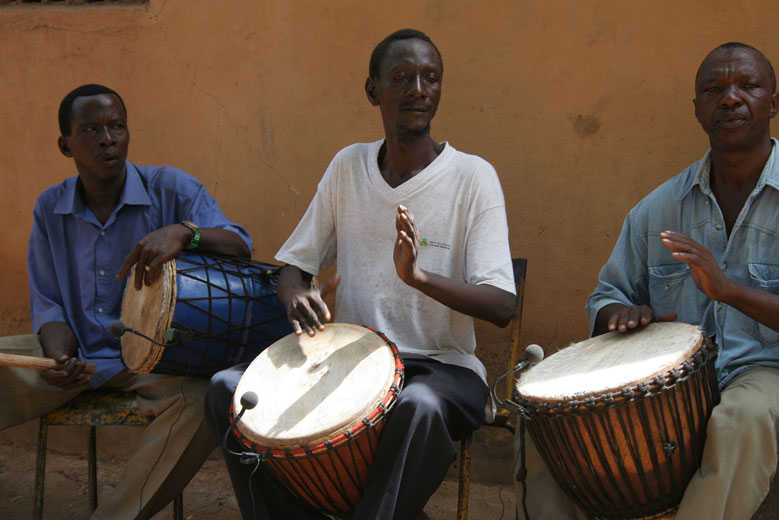
\includegraphics[width=0.5\linewidth]{figures/polak_ex1.jpg}
    \caption{Left: Dundun (Madu Jakite). Centre: Jembe 1 (Sedu Balo). Right: Jembe 2 (Drissa Kone). Reproduced from Polak \cite{polak2010}.}
    \label{fig:jembe_photo}
\end{figure}

The Viennese waltz is a style of music intended for ballroom dancing. It is a
fast waltz in \setmetre{3}{4} at around 180 beats per minute (bpm) and is performed by a
classical Western orchestra. It has a characteristic short-long-medium
micro-timing pattern for the length of its beats \cite{bengtsson1974,bengtsson1977}.




\chapter{Implementation} \label{implementation}

The implementation of this project consists of a few main components.

The first is the addition of the micro-timing functionality into Sonic Pi.
This consists of implementing musical metre, new commands to play music
within a metrical context, the style-specific micro-timing itself, and a method
of multi-threaded synchronisation. The second main component is the data
analysis which is used to generate realistic micro-timing for musical styles.
This is done primarily for Malian jembe, but also for Viennese waltz in
preparation for the evaluation and to check generalisability. The final component is a 
pair of converters between the MusicXML file format and my extended Sonic Pi language, 
also implemented for use in the evaluation.

This chapter details the data structures, algorithms, and approaches used to
implement these features.



\section{Metre} \label{metre_implementation}

Implementing a concept of musical metre within Sonic Pi was a crucial step
towards adding micro-timing functionality. Without it, the system has no way of
knowing where each note falls within the metrical cycle, and therefore no way of
knowing what timing adjustment it should apply. This section describes the way
the metrical hierarchy has been implemented as a tree data structure, and the
main algorithms which act on it. I then go on to describe the Bar class as a
representation of a single metrical cycle.


\subsection{Metrical hierarchy as trees} \label{metrical_hierarchy}

A tree data structure was chosen as a more descriptive representation for the
hierarchy information within a metre. This is a common way to depict metre;
Forth provides a detailed mathematical treatment of trees used in this context
\cite{forth2012}. To ensure an implementation that works well as part of a
programming language, I used the popular \verb'music21' Python library as a basis for
designing my representation \cite{ariza2010}.

The tree structure is implemented by the MetreLeaf and MetreTree classes (see
Sections~\ref{metreleaf} and~\ref{metretree} for more details). Figure~\ref{fig:tree_object_hierarchy} shows the default tree structure formed by these objects and their durations
for both a \setmetre{4}{4} time signature and an unconventional, pathological example metre. Note how the duration of a parent node is the sum of the durations of its children. Figure~\ref{fig:unconventional_metre_notation} shows some example music for the unconventional metre and how the grouping of notes in Western music notation is directed by the metrical hierarchy.

\begin{figure}[ht]
    \centering
    \begin{subfigure}{\linewidth}
        \centering
        \resizebox{\linewidth}{!}{
            \begin{forest}
                for tree=draw,
                [{\small \bfseries Metre \\ $d=1$}
                    [{\small \bfseries MetreTree \\ $d=\frac{1}{4}$}
                        [{\small \bfseries MetreLeaf \\ $d=\frac{1}{8}$}]
                        [{\small \bfseries MetreLeaf \\ $d=\frac{1}{8}$}]
                    ]
                    [{\small \bfseries MetreTree \\ $d=\frac{1}{4}$}
                        [{\small \bfseries MetreLeaf \\ $d=\frac{1}{8}$}]
                        [{\small \bfseries MetreLeaf \\ $d=\frac{1}{8}$}]
                    ]
                    [{\small \bfseries MetreTree \\ $d=\frac{1}{4}$}
                        [{\small \bfseries MetreLeaf \\ $d=\frac{1}{8}$}]
                        [{\small \bfseries MetreLeaf \\ $d=\frac{1}{8}$}]
                    ]
                    [{\small \bfseries MetreTree \\ $d=\frac{1}{4}$}
                        [{\small \bfseries MetreLeaf \\ $d=\frac{1}{8}$}]
                        [{\small \bfseries MetreLeaf \\ $d=\frac{1}{8}$}]
                    ]
                ]
            \end{forest}
        }
        \caption{Object hierarchy for \setmetre{4}{4}}
        \label{fig:tree_object_hierarchy_4_4}
    \end{subfigure}
    \\[1.5ex]
    \begin{subfigure}{\linewidth}
        \centering
        \resizebox{0.8125\linewidth}{!}{
            \begin{forest}
                for tree=draw,
                [{\small \bfseries Metre \\ $d=\frac{11}{8}$}
                    [{\small \bfseries MetreTree \\ $d=\frac{1}{4}$}
                        [{\small \bfseries MetreLeaf \\ $d=\frac{1}{8}$}]
                        [{\small \bfseries MetreLeaf \\ $d=\frac{1}{8}$}]
                    ]
                    [{\small \bfseries MetreTree \\ $d=\frac{1}{4}$}
                        [{\small \bfseries MetreLeaf \\ $d=\frac{1}{16}$}]
                        [{\small \bfseries MetreLeaf \\ $d=\frac{3}{16}$}]
                    ]
                    [{\small \bfseries MetreLeaf \\ $d=\frac{1}{8}$}]
                    [{\small \bfseries MetreTree \\ $d=\frac{3}{4}$}
                        [{\small \bfseries MetreLeaf \\ $d=\frac{1}{4}$}]
                        [{\small \bfseries MetreTree \\ $d=\frac{1}{2}$}
                            [{\small \bfseries MetreLeaf \\ $d=\frac{5}{16}$}]
                            [{\small \bfseries MetreLeaf \\ $d=\frac{3}{16}$}]
                        ]
                    ]
                ]
            \end{forest}
        }
        \caption{Object hierarchy for a pathological \setmetre{11}{8} metre}
        \label{fig:tree_object_hierarchy_unconventional}
    \end{subfigure}
    \caption{Two examples of how MetreTree and MetreLeaf objects are nested to construct metrical hierarchies for two different metres. The total duration $d$ of each node is also displayed, and the duration of a parent node is the sum of the durations of its children.}
    \label{fig:tree_object_hierarchy}
\end{figure}

\begin{figure}[ht]
    \centering
    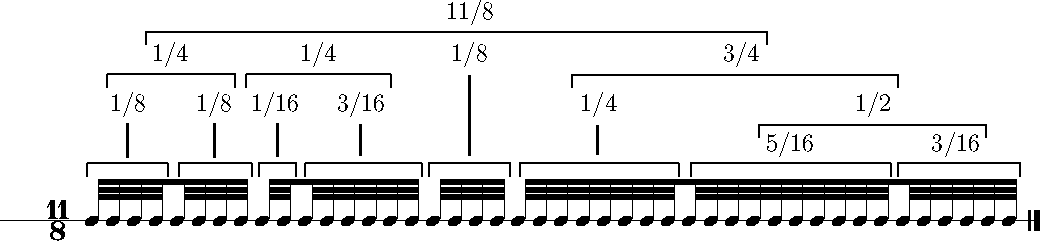
\includegraphics[width=\linewidth]{figures/hierarchy_notation_v2.pdf}
    \caption{One bar of music using the metre in Figure~\ref{fig:tree_object_hierarchy_unconventional}. Western music notation shows the hierarchy by the way it groups notes.}
    \label{fig:unconventional_metre_notation}
\end{figure}

The tree data structures can only have a finite depth, whereas metrical hierarchies are infinitely deep (otherwise we would not be able to represent notes with very short durations). Therefore, we have to make assumptions about the structure of the hierarchy for levels deeper than those defined by the data structure. In this case, we assume that each MetreLeaf is divided into two to get the next level.


\subsection{MetreLeaf class} \label{metreleaf}

A MetreLeaf object is the leaf node of the metrical tree structure. It has an
instance variable \verb'fraction' which represents the duration of the
MetreLeaf as a fraction of a whole note. This is stored as a Rational -- a Ruby object representing a rational number as a simplified fraction. For
example, a leaf node with the duration of one quarter note will have the value $\frac{1}{4}$.

The class contains a \verb'subdivide()' method, which divides the MetreLeaf by two a
given number of times, $s$. It returns a new MetreTree with $2^s$ MetreLeaf children, each of value $f/2^s$ where $f$ is the fraction of the original MetreLeaf.


\subsection{MetreTree class} \label{metretree}

A MetreTree object represents the hierarchical tree or subtree of a metre. The
instance variable \verb'sequence' is an ordered list representing this node's children and contains any combination of
MetreLeaf objects and other MetreTree objects. For
example, the previous example hierarchy in Figure~\ref{fig:tree_object_hierarchy_4_4} could also be written in list form as:
\[\left[\left[\frac{1}{8},\frac{1}{8}\right],\left[\frac{1}{8},\frac{1}{8}\right],\left[\frac{1}{8},\frac{1}{8}\right],\left[\frac{1}{8},\frac{1}{8}\right]\right]\]
Each list is a
MetreTree, and each fraction is a MetreLeaf. The MetreTree class contains
several methods for manipulating and extracting information from the metrical
hierarchy it represents. The two most important of these are explained in more
detail below.

\subsubsection{Getting metrical levels} \label{get_level}

Recall that the depth levels of a metrical hierarchy are called \emph{metrical levels} -- the basis of which is the beat level. The beat is divided to get \emph{division levels}, and grouped to get \emph{multiple levels}. A useful transformation on a MetreTree is to flatten the tree structure to a specified depth. This allows us to access the sequence of events at a given metrical level.

This is implemented by the \verb'get_level()' method, which returns a flat MetreTree at
a given metrical level $l$. A flat MetreTree is defined as one whose children are
only MetreLeafs, meaning there is no hierarchy (e.g.\ $\left[\frac{1}{8},\frac{1}{8},\frac{1}{8},\frac{1}{8},\frac{1}{8},\frac{1}{8},\frac{1}{8},\frac{1}{8}\right]$). Despite still being stored as a MetreTree object, it no longer represents a full metrical hierarchy, just one level of it.

This method is split into two algorithms:
\begin{itemize}
    \item \verb'get_division_level()' computes the sequence for division levels ($l>0$) and the beat level ($l=0$).
	\item \verb'get_multiple_level()' computes a possible sequence for multiple levels ($l<0$).
\end{itemize}

Algorithm~\ref{alg:getDivisionLevel} shows the \verb'get_division_level()' method. For each child in the
sequence list, if it is a MetreTree, the method is recursively called until the
base case of $l=0$ is reached. At this point, all the children of that node are
combined into one MetreLeaf equal to the sum of their durations. If the child is
instead a MetreLeaf, it is subdivided $l$ times to reach the desired metrical
level.

\begin{algorithm}[H]
    \SetKw{KwForIn}{in}
    \SetKwFunction{GetDivLevel}{get\_division\_level}

    \caption{get\_division\_level()}
    \KwIn{Target metrical level, $l$}
    \KwOut{New flat MetreTree at level $l$}
    \BlankLine

    new\_sequence $\gets$ empty list\;
    \ForEach{child \KwForIn @sequence}{
        \eIf{child is a MetreLeaf}{
            \eIf{$l>0$}{
                append (child subdivided $l$ times) to new\_sequence\;
            }{
                append child to new\_sequence\;
            }
        }{
            \tcp{child is a MetreTree}
            \eIf{$l>0$}{
                $r \gets$ recursive call to \GetDivLevel{$l-1$} method on child\;
                append $r$ to new\_sequence\;
            }{
                \tcp{Base of recursion}
                $m \gets$ combine all children of child into one MetreLeaf\;
                append $m$ to new\_sequence\;
            }
        }
    }
    \Return{new MetreTree made from new\_sequence}
    \label{alg:getDivisionLevel}
\end{algorithm}
\pagebreak

The \verb'get_multiple_level()' algorithm performs an estimate of the structure of
higher metrical levels by clustering nodes together. It is an estimate because this information is not in the
MetreTree's representation of the metre, so is just one possibility for the higher structure. The algorithm recursively clusters nodes until
the desired metrical level $l$ is reached. The number of nodes combined in each cluster is
determined by the smallest prime factor of the number of nodes at the level below. For
example, if level $l+1$ has four nodes, they will be clustered in groups of two. If it
has nine nodes, they will be clustered in groups of three.

An important consideration when implementing the \verb'get_level()' method was to
maximise its efficiency, because it is called often -- at least once per note. The
running time of the algorithm is $O(\left\lvert l\right\rvert)$, where $\left\lvert l\right\rvert$ is the number of MetreLeafs in the
hierarchy. To improve the efficiency, I implemented a cache of metrical levels for each
MetreTree object to store expensive computations for later reuse.

Some examples of the output of \verb'get_level()' for the following pathological hierarchy (from Figure~\ref{fig:tree_object_hierarchy_unconventional}) are shown in Table~\ref{table:get_level}:
\[
    \left[
        \left[\frac{1}{8},\frac{1}{8}\right],
        \left[\frac{1}{16},\frac{3}{16}\right],
        \frac{1}{8},
        \left[\frac{1}{4},\left[\frac{5}{16},\frac{3}{16}\right]\right]
    \right]
\]

\begin{table}[ht]
    \centering
    \renewcommand{\arraystretch}{2.0}
    \begin{tabular}{|c|c|}
        \hline
        $l$     & \verb'get_level'$(l)$ \\
        \hline
        $-2$    & $\displaystyle \left[ \frac{11}{8} \right]$ \\
        $-1$    & $\displaystyle \left[ \frac{1}{2},\frac{7}{8} \right]$ \\
        $0$     & $\displaystyle \left[ \frac{1}{4},\frac{1}{4},\frac{1}{8},\frac{3}{4} \right]$ \\
        $1$     & $\displaystyle \left[ \frac{1}{8},\frac{1}{8},\frac{1}{16},\frac{3}{16},\frac{1}{16},\frac{1}{16},\frac{1}{4},\frac{1}{2} \right]$ \\
        $2$     & $\displaystyle \left[ \frac{1}{16},\frac{1}{16},\frac{1}{16},\frac{1}{16},\frac{1}{32},\frac{1}{32},\frac{3}{32},\frac{3}{32},\frac{1}{32},\frac{1}{32},\frac{1}{32},\frac{1}{32},\frac{1}{8},\frac{1}{8},\frac{5}{16},\frac{3}{16} \right]$ \\ [1ex]
        \hline
    \end{tabular}
    \renewcommand{\arraystretch}{1.0}
    \cprotect\caption{Examples of the output of \verb'get_level'$(l)$ at different metrical levels $l$ for the hierarchy $[[1/8,1/8],[1/16,3/16],1/8,[1/4,[5/16,3/16]]]$. Note how level $l=-1$ is formed by the clustering of level $l=0$.}
    \label{table:get_level}
\end{table}

\subsubsection{Getting exact metrical events} \label{metrical_level_indices}

The second key method in the MetreTree class is \verb'metrical_level_indices()'. We define an \emph{offset} as a position in the metric cycle represented as the number of quarter lengths (the length of one quarter note) since the beginning of the cycle. For a
given offset, this algorithm finds any metrical events
which occur exactly at this offset, and returns their index.

Consider the example shown in Figure~\ref{fig:metrical_level_indices_example}. Offset $x$
occurs on the first event of all three levels, so the function would return $L_0(x)=L_1(x)=L_2(x)=0$, where $L_l(x)$ is the index of an event at level $l$ that offset $x$ occurs on. Offset $y$ occurs only on the last event of Level 1 and the second-to-last event of Level 2, so the function would return $L_1(y)=3, L_2(y)=6$.

This method is important because it
is used later to determine which micro-timing probability distributions should
be applied to a note at a given offset (see Section~\ref{applying_micro-timing}).

\begin{figure}[ht]
    \centering
    \resizebox{\linewidth}{!}{
        \begin{adjustbox}{valign=t}
            \begin{forest}
                for tree={no edge},
                [, [Level 0 [Level 1 [Level 2]]]]
            \end{forest}
        \end{adjustbox}\qquad
        \begin{adjustbox}{valign=t}
            \begin{forest}
                for tree={calign=first},
                [,phantom,name=Phantom1
                    [{$\frac{1}{4}$},name=First4
                        [{$\frac{1}{8}$}
                            [{$\frac{1}{16}$}]
                            [{$\frac{1}{16}$}]
                        ]
                        [{$\frac{1}{8}$}
                            [{$\frac{1}{16}$}]
                            [{$\frac{1}{16}$}]
                        ]
                    ]
                ]
                \node(xNode)[red] at (First4 |- Phantom1) {$x$};
                \draw[->,red] (xNode) to (First4);
            \end{forest}
        \end{adjustbox}\qquad
        \begin{adjustbox}{valign=t}
            \begin{forest}
                for tree={calign=first},
                [,phantom,name=Phantom2
                    [{$\frac{1}{4}$}
                        [{$\frac{1}{8}$}
                            [{$\frac{1}{16}$}]
                            [{$\frac{1}{16}$}]
                        ]
                        [{$\frac{1}{8}$},name=Last8
                            [{$\frac{1}{16}$}]
                            [{$\frac{1}{16}$}]
                        ]
                    ]
                ]
                \node(yNode)[red] at (Last8 |- Phantom2) {$y$};
                \draw[->,red] (yNode) to (Last8);
            \end{forest}
        \end{adjustbox}\qquad
    }
    \caption{An example metrical hierarchy for \setmetre{2}{4} showing which metrical events at each level (if any) offsets $x$ and $y$ occur on. $x$ occurs on the first event in all three levels. $y$ only occurs exactly on an event in Levels 1 and 2 -- namely events with indices 3 and 6, respectively.}
    \label{fig:metrical_level_indices_example}
\end{figure}


\subsection{Metre class} \label{metre_class}

The Metre class is a subclass of MetreTree which acts as a wrapper for the
hierarchy stored in a MetreTree. It implements functionality allowing a user to
specify a metre by a time signature string (e.g.\ \verb|'4/4'|) for common metres, or a
nested list of Rationals representing the hierarchy (e.g.\ \verb'[[1/8r,1/8r],[1/16r,3/16r],1/8r,[1/4r,[5/16r,3/16r]]]'). It also has a method which
converts a duration in quarter lengths to Sonic
Pi beats.


\subsection{Bar class} \label{bar_class}

A bar\footnote{Known as a \emph{bar} in British English, and a \emph{measure} in American English.} is a common term used in Western music theory for a single
metric cycle\footnote{A more precise definition would account for \emph{hypermetre}, where bars occur at the beat level \cite{neal2000}, but the simple definition is sufficient for our purposes.}. The Bar class is a representation of this, and each instance of it
has an associated metre. A Bar object is responsible for:
\begin{itemize}
	\item Keeping track of the playback position through the cycle (the \verb'current_offset' variable).
	\item Converting a note length given as a metrical level and a duration into
quarter lengths.
	\item Checking if a note or rest fits in the remaining time in the cycle, and
updating the bar's playback position accordingly.
\end{itemize}

A note's length is specified as a metrical level and a duration. The duration
is in units of an event at the specified metrical level, and acts as a multiplier.
For example, if a note's length is defined as $(l,d)=(0,3)$, its unit length is the duration of an event at level $l=0$, and it lasts for $d=3$ of these units.

The \verb'add_note()' method handles checking if a note fits into the bar, as shown in
Algorithm~\ref{alg:add_note}. If a note cannot fit into the bar's remaining time,
an exception is raised. This ensures the bar obeys the duration of its metre.

\begin{algorithm}[h]
    \SetKwFor{RepeatTimes}{repeat}{times do}{end}
    \SetKw{Raise}{raise}

    \caption{add\_note()}
    \KwIn{Metrical level, $l$}
    \KwIn{Duration, $d$}
    \KwIn{Total metre duration (in quarter lengths), $q$}
    \KwIn{Bar's current playback position, @current\_offset}
    \BlankLine

    new\_offset $\gets$ @current\_offset\;
    $M \gets$ metre flattened to level $l$\;
    \RepeatTimes{$d$}{
        \eIf{new\_offset $\geq q$}{
            \Raise CannotFitNoteException\;
        }{
            $n \gets$ length of active event in $M$ at new\_offset\;
            new\_offset $\gets \textnormal{new\_offset} + n$\;
        }
    }
    @current\_offset $\gets$ new\_offset\;
    \label{alg:add_note}
\end{algorithm}



\section{Playing music} \label{playing_music}

Now that the framework of musical metre has been established, we can look at how
this is used to play music. This section describes the new Sonic Pi
commands I have implemented for controlling metre, and adding notes and rests.
Figure~\ref{fig:sonicpi_language_comparison} shows a comparison between the original Sonic Pi commands (left), my
alternative commands (centre), and traditional Western music notation (right)
for a single bar of \setmetre{4}{4}.
\newpage

\begin{figure}[ht]
    \centering
    \begin{subfigure}[b]{0.2\textwidth}
        \centering
        \begin{minted}{ruby}
play :C4
sleep(1)
play :E4
sleep(1)
play :G4
sleep(0.5)
play :E4
sleep(0.5)
play :C4
        \end{minted}
        \caption{Old}
    \end{subfigure}
    %
    \begin{subfigure}[b]{0.4\textwidth}
        \centering
        \begin{minted}{ruby}
use_metre '4/4'

bar do
    add_note :C4, 0, 1
    add_note :E4, 0, 1
    add_note :G4, 1, 1
    add_note :E4, 1, 1
    add_note :C4, 0, 1
end
        \end{minted}
        \caption{New}
    \end{subfigure}
    %
    \begin{subfigure}[b]{0.3\textwidth}
        \centering
        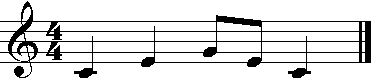
\includegraphics[width=\linewidth]{figures/sonic_pi_comparison.pdf}
        \caption{Notation}
    \end{subfigure}
    \cprotect\caption{A single bar of music represented by the original Sonic Pi syntax, my new metre commands, and traditional Western music notation. Note how the original Sonic Pi syntax loses information about the metre. The second and third arguments to \verb'add_note' are the metrical level and duration.}
    \label{fig:sonicpi_language_comparison}
\end{figure}


\subsection{Metre commands} \label{metre_commands}

A metre is created with the \verb'use_metre' or \verb'with_metre' commands. These have been
designed to match the syntax of existing Sonic Pi commands such as \verb'use_fx' and \verb'with_fx'. Sonic Pi uses multiple threads of execution to allow different musical parts to play simultaneously. Each of these commands operates only within its current thread. See Section~\ref{multi-threaded_synchronisation} for more on multi-threading.

\begin{itemize}
	\item \verb'use_metre('$m$\verb')' changes the current thread's metre to $m$ (using a thread-local variable).
	\item \verb'with_metre('$m$\mintinline{ruby}|) bar do ... end| executes a block of user code with a specified metre $m$, then restores the thread's original metre.
\end{itemize}

The \mintinline{ruby}|bar do ... end| command creates a new Bar object, stores this to a
thread-local variable, then executes a block of user code. If the Bar object
still has space remaining after the block has run, the function then sleeps for
the appropriate time.


\subsection{Sound commands} \label{sound_commands}

There are three main sound commands: \verb'add_note', \verb'add_sample', and \verb'add_rest'. A
user can use \verb'add_note' to play a note on the current synthesiser. A note is
defined as a pitch (how high or low it sounds) and a length. The pitch is
specified as in Sonic Pi's \verb'play' command, such as by a note name and octave (C4)
or a MIDI note (60). A list of pitches will sound together as a chord. The
length is given as a metrical level and a duration, as defined in Section~\ref{bar_class}.

The \verb'add_note' command works as follows:
\begin{enumerate}
    \item Gets the current Bar object from the thread-local variables.
    \item Calls the Bar's \verb'add_note()' method to check if the note will fit into the current bar.
    \item Passes the note pitch to Sonic Pi's \verb'play' function which creates the sound.
    \item Sleeps for the duration of the note.
\end{enumerate}

I have also implemented some shorthand commands such as \verb'add_quarter' and
\verb'add_whole' which act as wrappers around calls to \verb'add_note'. This was done to
provide an easy-to-use alternative to the metrical level notation for users who
are less familiar with Western music theory. This was especially important as
Sonic Pi was designed to be accessible to schoolchildren \cite{aaron2013}.

The final two sound commands are \verb'add_sample' and \verb'add_rest'. These function the
same as \verb'add_note', except \verb'add_sample' plays an audio sample and \verb'add_rest' simply sleeps.



\section{Micro-timing} \label{micro-timing_implementation}

In order to add micro-timing functionality to my implementation, I first needed
a way of representing and storing the micro-timing information for different
musical styles. This information is represented by probability distributions for
each event in a metric cycle, describing how early or late each event should
occur. In this section, I describe how the
Style class stores the micro-timing information for a musical style, and how
this is used to apply micro-timing to a user's music.


\subsection{Style class} \label{style_class}

The Style class stores micro-timing values as a Hash from metrical levels (0, 1,
etc.) to lists containing one probability distribution object for each event at
that level. It will accept any distribution object which has a \verb'sample()' method,
such as my NormalDistribution class described below.

For example, a Style object with the Hash shown below defines micro-timing only for metrical level
$l=0$ (the beat level) for a metre with three beats. The first beat is played exactly on time,
with no variance. The second beat is early, with normal distribution $(\mu,\sigma)=(-0.3,0.01)$.
The third beat is very slightly late, with normal distribution $(\mu,\sigma)=(0.001,0)$.

\begin{minted}{ruby}
{
    0 => [
        NormalDistribution.new(0,0),
        NormalDistribution.new(-0.3, 0.01),
        NormalDistribution.new(0.001,0)
    ]
}
\end{minted}

The class also has a test to see if the style is compatible with a given metrical
hierarchy. A Style is defined as being compatible with a MetreTree if, for each
metrical level defined in the Style, it has exactly one distribution for each
metrical event at that level in the MetreTree.

\subsubsection{NormalDistribution class} \label{normal_distribution}

I have implemented a NormalDistribution class, which is initialised with a mean $\mu$ and standard deviation
$\sigma$, and has a method for generating random samples.

Samples are generated using the
Box-Muller transform \cite{box1958}, which transforms a pair of uniform random
samples into a pair of normally distributed samples. Sonic Pi's random number
generator is used for the uniform random samples. This is because it generates a
deterministic, repeatable sequence of pseudorandom numbers, which means the output of
a Sonic Pi program sounds the same each time it is run \cite{aaron2016}.


\subsection{Applying micro-timing} \label{applying_micro-timing}

When a user sets a metre with the \verb'use_metre' or \verb'with_metre' commands, they can
specify an optional second argument as either a Style object or the name of a
style to be looked up, as shown below. This causes all music played with that metre to use the micro-timing of the chosen style.
\begin{minted}{ruby}
use_metre '12/8', :jembe
use_metre '4/4', Style.new("example", {0 => [...]})
\end{minted}

At the start of each new bar, the Metre object samples new values from the
Style's probability distributions. When a note is played inside the bar, the
\verb'add_note' command requests the timing shift that should be applied to the note
from the Metre. To calculate this, the Metre object calls its
\verb'metrical_level_indices()' method (see Section~\ref{metrical_level_indices}) to determine which timing
values from each level to use. The individual timing contributions of each
metrical level are summed to produce an overall timing shift for the
note. A positive value means the note should be played slightly late; a negative
value means slightly early. This is returned to \verb'add_note' which then uses Sonic Pi's \verb'time_warp' function (see Section~\ref{live_coding_background}) to adjust the timing of the call to \verb'play'.

For example, if the sampled timings, $T_l$, for each level, $l$, are:
\begin{equation*}
    \begin{split}
        T_0 &= [0,0.1] \\
        T_1 &= [0.03,0,0,-0.02]
    \end{split}
\end{equation*}
and the metrical level indices, $L_l$, for each level, $l$, are:
\begin{equation*}
    \begin{split}
        L_0 &= 1 \\
        L_1 &= 3
    \end{split}
\end{equation*}
then the timing shift, $t$, would be calculated by:
\begin{equation*}
    \begin{split}
        t &= \sum_{i \in T.\mathrm{keys}} T_i[L_i] \\
        &=T_0[L_0]+T_1[L_1] \\
        &=0.1+(-0.02) \\
        &=0.08
    \end{split}
\end{equation*}
Therefore, the note will be played 0.08 quarter lengths late.



\section{Multi-threaded synchronisation} \label{multi-threaded_synchronisation}

An important part of producing music in Sonic Pi is the ability to have multiple
instruments/parts playing simultaneously. This is accomplished by having
separate threads of execution. Aaron et al.'s previous work on Sonic Pi's
temporal semantics ensures music in separate threads remains in time \cite{aaron2014}.
Because of the probabilistic nature of my micro-timing implementation, each
thread needs to have the same set of randomly generated timing values to remain
perfectly synchronised. Otherwise, notes in different threads that are supposed
to sound at the same moment might not do so. To tackle this, I implemented a
SynchronisedMetre class which generates new random timing values exactly once
per bar.


\subsection{SynchronisedMetre class} \label{synchronised_metre}

The SynchronisedMetre class is a subclass of Metre which is designed to control
the synchronisation of all the notes contained in the metre. Its main functions,
in addition to those of the Metre class, are to:
\begin{itemize}
	\item Set a Style to use for generating micro-timing values.
	\item Sample from the Style's probability distributions to get timing values.
	\item Compute the total timing shift to be applied to a note at a given offset.
	\item Ensure all Bar objects which use it remain synchronised and all have the same set of timing values.
\end{itemize}


\subsection{Bar number synchronisation} \label{bar_number_synchronisation}

To make sure Bar objects in separate threads all have the same micro-timing
values, and that these values are regenerated exactly once per cycle, I
synchronise the Bars on the current `bar number'. This is a counter of the
number of bars that have occurred since the beginning of playback. The behaviour
of the Bar class is as follows:

\begin{minted}{ruby}
class Bar
    def initialize()
        previous_bar_number = __thread_locals.get(:sonic_pi_bar_number)
        if previous_bar_number
            current_bar_number = @metre.request_bar(previous_bar_number + 1)
        else
            current_bar_number = @metre.request_bar(0)
        end
        __thread_locals.set(:sonic_pi_bar_number, current_bar_number)
    end
end
\end{minted}

If this is the first bar in the thread, the Bar object will request bar number 0
from the metre, otherwise it will request the next bar number in sequence. The
metre returns the actual current bar number, which is then stored in the thread
locals for the next bar to use.

\begin{minted}{ruby}
class SynchronisedMetre < Metre

    def initialize()
        @timings = recalculate_timings()
        @current_bar_number = 0
        @mutex = Mutex.new()
    end

    def request_bar(requested_bar_number)
        @mutex.synchronise do
            if requested_bar_number > @current_bar_number
                @timings = recalculate_timings()
                @current_bar_number = requested_bar_number
            end
        end
        return @current_bar_number
    end
end
\end{minted}

The SynchronisedMetre's \verb'request_bar()' method determines the correct current bar
number. If the requested number is greater than its internal current number,
then it must be the start of a new bar. So, the timings are recalculated, and
its current bar number is updated. If the requested number is old, then it just
returns the current number. The method is synchronised on a mutex to avoid any
race conditions which might cause bars to get different timing values.

\usetikzlibrary{positioning}
\begin{figure}[ht]
    \centering
    \begin{tikzpicture}[node distance=4]
        \node[] (Metre) {SynchronisedMetre};
        \node[right = of Metre] (Thread1) {Thread 1};
        \node[right = of Thread1] (Thread2) {Thread 2};
        \node[below of=Metre, node distance=7cm] (Metre_ground) {};
        \node[below of=Thread1, node distance=7cm] (Thread1_ground) {};
        \node[below of=Thread2, node distance=7cm] (Thread2_ground) {};
        %
        \draw (Metre) -- (Metre_ground);
        \draw (Thread1) -- (Thread1_ground);
        \draw (Thread2) -- (Thread2_ground);
        \draw[->] (Thread1 |- 0,-1) -- node[above,sloped,midway]{requestBar(0)} node[at start,right]{0} node[at end,left]{0} (Metre |- 0,-2);
        \draw[->] (Metre |- 0,-2) -- node[above,sloped,midway]{$b=0$} node[at end,right]{0} (Thread1 |- 0,-2.5);
        \draw[->] (Thread1 |- 0,-3) -- node[above,sloped,midway]{requestBar(1)} node[at end,left]{1} (Metre |- 0,-4);
        \draw[->] (Metre |- 0,-4) -- node[above,sloped,midway]{$b=1$} node[at end,right]{1} (Thread1 |- 0,-4.5);
        \draw[->] (Thread2 |- 0,-5) -- node[above,sloped,midway]{requestBar(0)} node[at start,right]{0} node[at end,left]{1} (Metre |- 0,-6);
        \draw[->] (Metre |- 0,-6) -- node[above,sloped,midway]{$b=1$} node[at end,right]{1} (Thread2 |- 0,-6.5);

    \end{tikzpicture}
    \caption{Sequence diagram demonstrating the behaviour of bar number synchronisation with multiple threads. Values along the vertical axes show that thread's bar number counter. Arrows represent method calls and their return values.}
    \label{fig:multi-threading_sequence_diagram}
\end{figure}
\pagebreak

Figure~\ref{fig:multi-threading_sequence_diagram} is a sequence diagram demonstrating the behaviour of the synchronisation
in the presence of multiple threads. Each object/thread's bar number counter is
shown along its axis. Each thread's counter is initialised to 0. Thread 1
requests bar 0, which is equal to the SynchronisedMetre's current value, so $b=0$
is returned. Thread 1 then requests the next bar number (1). This is greater
than the SynchronisedMetre's current value, so its value is updated and returned.
Thread 2 then starts late and requests an old bar number (0). The
SynchronisedMetre recognises this is old, so simply returns its current value
$b=1$ so Thread 2 can catch up.



\section{Jembe data analysis} \label{jembe_data_analysis}

Creating music with realistic micro-timing using the implementation I have
described requires a set of probability distributions which accurately
characterise a style of music. Therefore, these distributions must be derived
from real-life examples of music. The next two sections describe the data
collection and analysis that was done for the jembe and Viennese waltz styles.
The results of the data analysis methods described here can be found in
Section~\ref{data_analysis_results}.


\subsection{Datasets} \label{jembe_datasets}

Previous research into the micro-timing of Malian jembe music has meant there
are some high-quality datasets of processed live recordings available.

The first dataset is from Jacoby et al.\ \cite{jacoby2021} and consists of 11
processed recordings of a piece called `Suku', which is a very commonly played
piece in this style. The second dataset is from the Interpersonal Entrainment in Music Performance
(IEMP) Data Collection \cite{polak2020,clayton2021}. This consists of 15 recordings
across three different pieces: `Manjanin', `Maraka', and `Woloso'. Both datasets here use recordings made by Rainer Polak in Mali -- see Appendix~\ref{appendix_datasets_jembe} for more recording details and a list of performers.

The datasets supply the following data:
\begin{itemize}
	\item Onset time -- the time when a drum stroke occurs
	\item Cycle number
	\item Metric location -- which metrical event the onset belongs to
	\item Phase -- the actual timing of the onset within the cycle
\end{itemize}


\subsection{Micro-timing estimation} \label{jembe_micro-timing}

The pieces of jembe music in the dataset use a metre\footnote{See Polak \cite{polak2010} for an ethnographically sensitive discussion of the extent to which metre applies in this context.} with four beats, each of
which divides into three, for a total of 12 metrical events at the first division
level (\setmetre{12}{8} in Western classical notation). It is at this level, referred to as the `pulse', that the micro-timing occurs.

Each event at the pulse level has a position in the cycle at which a note would
occur if it were isochronous (the \emph{categorical} timing). The displacement from this position describes the
micro-timing (or \emph{expressive} timing) of the note, and this is what is stored in the probability
distributions described in Section~\ref{style_class}. Equation~\ref{eq:displacement_from_phase} shows how the displacement is calculated from the phase given by the datasets.
\begin{equation}
    \textnormal{displacement} = \frac{(\textnormal{phase} \times \textnormal{beat division}) - \textnormal{metric location}}{2}
    \label{eq:displacement_from_phase}
\end{equation}
The phase is multiplied by the beat division (in this case, 3) to convert it
into pulse units. The metric location at the pulse level (an integer from 0 to 11)
is subtracted to get the displacement. The final division by two converts the displacement
into quarter lengths (because each pulse unit is an eighth length).

For example, if an onset has metric location $=6$ and phase $=2.01$, the displacement would be calculated by:
\[\textnormal{displacement} = \frac{(2.01 \times 3) - 6}{2} = \frac{0.03}{2} = 0.015 \textnormal{ quarter lengths}\]

Once the displacement has been calculated for each drum stroke, I was then able to
estimate the distribution of displacements for each of the twelve metric locations. I
considered two types of approach for this probability density estimation:

\begin{itemize}
	\item Kernel density estimation (KDE) (non-parametric) -- applies smoothing to the
data to fit an arbitrary distribution.
	\item Maximum likelihood estimation (MLE) (parametric) -- estimates the parameters of a given existing distribution which best fit the data.
\end{itemize}

The advantage of KDE is that it would be able to accurately represent any shape
of distribution the data may have. However, each point in
the probability density function has to be stored individually. This means it generally has a higher memory
requirement than MLE, which only stores the values of the parameters. Another
advantage of MLE is it allows hypothetical distributions to be easily defined
without the need for data.

For this scenario, I chose to use MLE to fit a normal distribution to the data.
A normal distribution was suitable because the data was assumed to be estimating
a theoretical true value of the displacement. A normal distribution requires two
parameters: the mean, $\mu$, and the standard deviation, $\sigma$. It can be shown that the maximum likelihood estimator $\hat{\mu}$ for the population mean is the sample mean $\bar{x}$, and the estimator $\hat{\sigma}$ for the population standard deviation is the sample standard deviation $s$ \cite{dekking2005}. The calculation of $s$ uses Bessel's
correction to get an unbiased estimator of $\hat{\sigma}$ \cite{upton2014}.


\subsection{Tempo estimation} \label{tempo_estimation}

Generating a synthetic piece of jembe music requires analysis of other musical
features as well as the micro-timing to sound realistic. One of these is the
\emph{tempo} (how fast or slow the beat is), which is measured in beats per minute
(bpm). The tempo of a jembe piece of music typically increases substantially
over the duration of the performance \cite{jacoby2021}, with the last 15 seconds or
so showing the tempo increasing at a much faster rate.

The \emph{inter-beat interval} (IBI) is defined as the time between two consecutive beats in a
piece of music, from which the instantaneous tempo can be calculated \cite{dixon2001}.
A moving average can be applied to the instantaneous tempo to obtain an estimate
of the global tempo.

For the jembe data, I first filtered all the onsets to include just those played
by Jembe 2 (because it plays on every beat \cite{jacoby2021}), then filtered these to
just onsets on the beats. I then calculated the inter-beat interval using Equation~\ref{eq:ibi}, where $b_i$ is the onset time of the $i$th beat. This is then converted to bpm by Equation~\ref{eq:tempo}. A moving average with window size 10 is then applied to smooth the tempo estimate.
\begin{equation}
    \mathrm{IBI}_i = b_i - b_{i-1}
    \label{eq:ibi}
\end{equation}
\begin{equation}
    t_i = \frac{60}{\mathrm{IBI}_i}
    \label{eq:tempo}
\end{equation}
Inspection of the smoothed tempo graphs (Section~\ref{jembe_tempo_estimation_results}) showed a logarithmic trend for the first $\sim95\%$ of the piece. A sharper increase follows this which was
modelled by a quadratic curve. To fit curves to the data, I used the \verb'optimize.curve_fit' function from the SciPy Python library, which uses a non-linear least
squares method \cite{more1977}. The parameters estimated by the curve fitting are then used in Sonic Pi
to control the tempo of a synthetic jembe piece during playback.


\subsection{Rhythm patterns} \label{rhythm_patterns}

The final data analysis performed on the jembe music was an analysis of the
rhythm patterns played by Jembe 1. While the other instruments in the ensemble
play repetitive accompaniments, Jembe 1 has a lead role and can play a variety
of rhythmic patterns, also often involving improvisation. By analysing these
patterns, I was able to produce a synthetic Jembe 1 part for Suku with
semi-realistic rhythms. My approach was as follows:

\begin{enumerate}
    \item Compute the rhythm played by Jembe 1 in each cycle as a 12-bit binary number, where the bit value at each position indicates whether there was an onset at the corresponding pulse in that cycle.
    \item Convert the 12-bit binary numbers into a unique decimal integer for each cycle.
    \item Count the number of times rhythm $x$ is followed by rhythm $y$ and calculate transition probabilities from these.
    \item Generate a random sequence of rhythm integers using the transition probabilities.
    \item During playback, for each cycle, play a drum stroke on pulse $i$ if there is a 1 at bit $i$ in the binary representation of that cycle's rhythm integer.
\end{enumerate}

This approach was an improvement over purely random rhythms because it preserved
intra-cycle patterns. The jembe can be played with three different techniques,
each producing a different kind of sound (timbre). These are tone, slap, and
bass. To include this, I created a roughly typical pattern covering each note
position in the cycle: [T,T,S,T,T,S,B,B,S,B,B,S]. If a note is played at a
particular pulse, the corresponding timbre is looked up from this pattern.



\section{Waltz data analysis} \label{waltz_data_analysis}

The Viennese waltz provides a useful comparison to Malian jembe in evaluating
this project's micro-timing implementation. This style uses a metre with three
beats (\setmetre{3}{4}) and the micro-timing can be observed at the beat level, where the
second beat is usually early. The micro-timing in Viennese waltz has not been
studied in as much detail or as recently as jembe, so there were no existing
datasets of Viennese waltz performances with micro-timing. This meant further
calculations were needed to derive it, which are explained in this section.


\subsection{Datasets} \label{waltz_datasets}

I first considered using the Ballroom dataset \cite{gouyon2006}, which contains
30-second recordings of 65 pieces of Viennese waltz music, and for which
annotations of the beats exists \cite{krebs2013}. However, when I listened to the
recordings, I did not notice any micro-timing. To test my suspicions, I performed
the micro-timing analysis described in Section~\ref{waltz_micro-timing} and then conducted a
one-sample \textit{t}-test. This tests whether the sample mean of the displacement of the
second beat is statistically significantly different from 0 (the case where
there is no micro-timing). At the 5\% significance level, there were very few
recordings which had any significant micro-timing, so this dataset was deemed
unsuitable.

I then constructed my own dataset comprising of 30-second samples from seven
waltz recordings performed by the Vienna Philharmonic Orchestra, all of which
have noticeable and statistically significant micro-timing. See Appendix~\ref{appendix_datasets_waltz} for more details. Because this dataset
has no existing beat annotations, the next step was to produce my own.


\subsection{Beat tracking} \label{beat_tracking}

\emph{Beat tracking} is the process of identifying the locations of beats in an audio
recording of a piece of music. Since the beat level is where the micro-timing in
the Viennese waltz occurs, no additional onset detection was necessary. The beat
tracking could be approached automatically with existing beat tracking
algorithms, or manually.

A variety of automatic beat tracking algorithms were tried, but most did not
perform well. Many implementations struggled because they expect the beats to be
isochronous, i.e.\ having no systematic micro-timing, as is the case in most
Western music. As a result, they would often skew the detected beats towards
being isochronous, therefore not capturing the micro-timing. Of all these
implementations, the beat tracking in the libfmp Python library \cite{mueller2021} (a
dynamic programming approach introduced by Müller \cite{mueller2021b}) performed the best. After some
small manual corrections, the beat onsets were ready for analysis, as described
in Section~\ref{waltz_micro-timing}.

As an alternative, manual beat annotations were created by hand using the Sonic
Visualiser software \cite{cannam2010}. While the micro-timing from this approach was
more prominent, the data had a large variance (likely due to human imprecision) which led to the generated music sounding erratic. For this reason, the automatic approach was chosen.


\subsection{Micro-timing estimation} \label{waltz_micro-timing}

To calculate the micro-timing displacement of each beat from just the onset time
involves first identifying the start and end of each cycle, estimating the onset
of each beat as if they were isochronous, then finding the difference between this
and the actual onset to get the displacement. The full calculation is shown in
Equation~\ref{eq:displacement_from_onset}, where $i$ ranges over the indices of all the onsets in the piece.
\begin{equation}
\begin{split}
    \mathrm{metricLocation}_i &= i \;\mathrm{mod}\; 3 \\
    \mathrm{cycleStart}_i     &= \mathrm{onset}_{i-\mathrm{metricLocation}_i} \\
    \mathrm{cycleEnd}_i       &= \mathrm{onset}_{i-\mathrm{metricLocation}_i+3} \\
    \mathrm{cycleDuration}_i  &= \mathrm{cycleEnd}_i - \mathrm{cycleStart}_i \\
    \mathrm{isochronousBeatDuration}_i &= \frac{\mathrm{cycleDuration}_i}{3} \\
    \mathrm{isochronousOnset}_i &= \mathrm{cycleStart}_i + (\mathrm{metricLocation}_i \times \mathrm{isochronousBeatDuration}_i) \\
    \mathrm{displacement}_i &= \frac{\mathrm{onset}_i-\mathrm{isochronousOnset}_i}{\mathrm{isochronousBeatDuration}_i} \\
    \mathrm{phase}_i          &= \mathrm{displacement}_i + \mathrm{metricLocation}_i
\end{split}
\label{eq:displacement_from_onset}
\end{equation}
The data is assumed to have exactly one onset for each beat in the piece, and the
duration of a cycle is assumed to be the time between its first beat and the
first beat of the next cycle.

Once the displacements had been derived, maximum
likelihood estimation was used to fit the probability distributions, as described in
Section~\ref{jembe_micro-timing}.
\newpage




\chapter{Evaluation} \label{evaluation}

This chapter aims to demonstrate the capabilities of my project and prove the
achievement of the success criteria.

I begin by showing the results of the
data analysis which was conducted as part of the implementation. This is a
crucial step towards being able to produce music with realistic micro-timing
because it provides the data needed to populate the styles' probability
distributions. Secondly, I describe the motivation, methods, and results of
a user study I conducted to evaluate how realistic the generated music sounds.
This includes a detailed description of how the study was carried out, how the
stimuli were constructed, and the full results. The section concludes with a
discussion of the results and their significance. Finally, I use the MusicXML
converters implemented earlier to demonstrate the value gained by an
implementation of metre within Sonic Pi and showcase its successful use.



\section{Data analysis results} \label{data_analysis_results}

This section displays the results of the data analysis described in Sections~\ref{jembe_data_analysis} and~\ref{waltz_data_analysis}. I
begin by describing the data-derived micro-timing for jembe and Viennese waltz,
and the patterns which occur in them. Jembe is found to have a short-medium-long
pattern in its pulses, and the waltz has a significantly early second beat. I
then describe the results of the jembe tempo estimation.


\subsection{Micro-timing estimation} \label{micro-timing_estimation_results}

Figure~\ref{fig:suku_histogram} shows the results of the micro-timing estimation (Section~\ref{jembe_micro-timing}) for one of
the jembe pieces, `Suku'. The histograms show the positions within the cycle
where each of the 12 pulses occurred (phase). The dashed lines show where the
event would occur if they were isochronous, so the existence of the micro-timing
can be seen clearly by the positions of the second and third pulses in each beat.
By examining the positions of the histograms, we can see that the length of each pulse follows a short-medium-long pattern (SML), which is consistent across
each beat. Also shown are the probability density functions (PDF) of the
maximum-likelihood estimated normal distributions. The plots for
the other jembe pieces showed the same pattern.

\begin{figure}[ht]
    \centering
    %% Creator: Matplotlib, PGF backend
%%
%% To include the figure in your LaTeX document, write
%%   \input{<filename>.pgf}
%%
%% Make sure the required packages are loaded in your preamble
%%   \usepackage{pgf}
%%
%% and, on pdftex
%%   \usepackage[utf8]{inputenc}\DeclareUnicodeCharacter{2212}{-}
%%
%% or, on luatex and xetex
%%   \usepackage{unicode-math}
%%
%% Figures using additional raster images can only be included by \input if
%% they are in the same directory as the main LaTeX file. For loading figures
%% from other directories you can use the `import` package
%%   \usepackage{import}
%%
%% and then include the figures with
%%   \import{<path to file>}{<filename>.pgf}
%%
%% Matplotlib used the following preamble
%%
\begingroup%
\makeatletter%
\begin{pgfpicture}%
\pgfpathrectangle{\pgfpointorigin}{\pgfqpoint{6.358179in}{1.754691in}}%
\pgfusepath{use as bounding box, clip}%
\begin{pgfscope}%
\pgfsetbuttcap%
\pgfsetmiterjoin%
\definecolor{currentfill}{rgb}{1.000000,1.000000,1.000000}%
\pgfsetfillcolor{currentfill}%
\pgfsetlinewidth{0.000000pt}%
\definecolor{currentstroke}{rgb}{1.000000,1.000000,1.000000}%
\pgfsetstrokecolor{currentstroke}%
\pgfsetdash{}{0pt}%
\pgfpathmoveto{\pgfqpoint{-0.000000in}{0.000000in}}%
\pgfpathlineto{\pgfqpoint{6.358179in}{0.000000in}}%
\pgfpathlineto{\pgfqpoint{6.358179in}{1.754691in}}%
\pgfpathlineto{\pgfqpoint{-0.000000in}{1.754691in}}%
\pgfpathclose%
\pgfusepath{fill}%
\end{pgfscope}%
\begin{pgfscope}%
\pgfsetbuttcap%
\pgfsetmiterjoin%
\definecolor{currentfill}{rgb}{1.000000,1.000000,1.000000}%
\pgfsetfillcolor{currentfill}%
\pgfsetlinewidth{0.000000pt}%
\definecolor{currentstroke}{rgb}{0.000000,0.000000,0.000000}%
\pgfsetstrokecolor{currentstroke}%
\pgfsetstrokeopacity{0.000000}%
\pgfsetdash{}{0pt}%
\pgfpathmoveto{\pgfqpoint{0.445679in}{0.499691in}}%
\pgfpathlineto{\pgfqpoint{6.258179in}{0.499691in}}%
\pgfpathlineto{\pgfqpoint{6.258179in}{1.654691in}}%
\pgfpathlineto{\pgfqpoint{0.445679in}{1.654691in}}%
\pgfpathclose%
\pgfusepath{fill}%
\end{pgfscope}%
\begin{pgfscope}%
\pgfpathrectangle{\pgfqpoint{0.445679in}{0.499691in}}{\pgfqpoint{5.812500in}{1.155000in}}%
\pgfusepath{clip}%
\pgfsetbuttcap%
\pgfsetmiterjoin%
\definecolor{currentfill}{rgb}{0.121569,0.466667,0.705882}%
\pgfsetfillcolor{currentfill}%
\pgfsetfillopacity{0.700000}%
\pgfsetlinewidth{0.000000pt}%
\definecolor{currentstroke}{rgb}{0.000000,0.000000,0.000000}%
\pgfsetstrokecolor{currentstroke}%
\pgfsetstrokeopacity{0.700000}%
\pgfsetdash{}{0pt}%
\pgfpathmoveto{\pgfqpoint{0.709884in}{0.499691in}}%
\pgfpathlineto{\pgfqpoint{0.719292in}{0.499691in}}%
\pgfpathlineto{\pgfqpoint{0.719292in}{0.503172in}}%
\pgfpathlineto{\pgfqpoint{0.709884in}{0.503172in}}%
\pgfpathclose%
\pgfusepath{fill}%
\end{pgfscope}%
\begin{pgfscope}%
\pgfpathrectangle{\pgfqpoint{0.445679in}{0.499691in}}{\pgfqpoint{5.812500in}{1.155000in}}%
\pgfusepath{clip}%
\pgfsetbuttcap%
\pgfsetmiterjoin%
\definecolor{currentfill}{rgb}{0.121569,0.466667,0.705882}%
\pgfsetfillcolor{currentfill}%
\pgfsetfillopacity{0.700000}%
\pgfsetlinewidth{0.000000pt}%
\definecolor{currentstroke}{rgb}{0.000000,0.000000,0.000000}%
\pgfsetstrokecolor{currentstroke}%
\pgfsetstrokeopacity{0.700000}%
\pgfsetdash{}{0pt}%
\pgfpathmoveto{\pgfqpoint{0.719292in}{0.499691in}}%
\pgfpathlineto{\pgfqpoint{0.728701in}{0.499691in}}%
\pgfpathlineto{\pgfqpoint{0.728701in}{0.506653in}}%
\pgfpathlineto{\pgfqpoint{0.719292in}{0.506653in}}%
\pgfpathclose%
\pgfusepath{fill}%
\end{pgfscope}%
\begin{pgfscope}%
\pgfpathrectangle{\pgfqpoint{0.445679in}{0.499691in}}{\pgfqpoint{5.812500in}{1.155000in}}%
\pgfusepath{clip}%
\pgfsetbuttcap%
\pgfsetmiterjoin%
\definecolor{currentfill}{rgb}{0.121569,0.466667,0.705882}%
\pgfsetfillcolor{currentfill}%
\pgfsetfillopacity{0.700000}%
\pgfsetlinewidth{0.000000pt}%
\definecolor{currentstroke}{rgb}{0.000000,0.000000,0.000000}%
\pgfsetstrokecolor{currentstroke}%
\pgfsetstrokeopacity{0.700000}%
\pgfsetdash{}{0pt}%
\pgfpathmoveto{\pgfqpoint{0.728701in}{0.499691in}}%
\pgfpathlineto{\pgfqpoint{0.738110in}{0.499691in}}%
\pgfpathlineto{\pgfqpoint{0.738110in}{0.520577in}}%
\pgfpathlineto{\pgfqpoint{0.728701in}{0.520577in}}%
\pgfpathclose%
\pgfusepath{fill}%
\end{pgfscope}%
\begin{pgfscope}%
\pgfpathrectangle{\pgfqpoint{0.445679in}{0.499691in}}{\pgfqpoint{5.812500in}{1.155000in}}%
\pgfusepath{clip}%
\pgfsetbuttcap%
\pgfsetmiterjoin%
\definecolor{currentfill}{rgb}{0.121569,0.466667,0.705882}%
\pgfsetfillcolor{currentfill}%
\pgfsetfillopacity{0.700000}%
\pgfsetlinewidth{0.000000pt}%
\definecolor{currentstroke}{rgb}{0.000000,0.000000,0.000000}%
\pgfsetstrokecolor{currentstroke}%
\pgfsetstrokeopacity{0.700000}%
\pgfsetdash{}{0pt}%
\pgfpathmoveto{\pgfqpoint{0.738110in}{0.499691in}}%
\pgfpathlineto{\pgfqpoint{0.747519in}{0.499691in}}%
\pgfpathlineto{\pgfqpoint{0.747519in}{0.513615in}}%
\pgfpathlineto{\pgfqpoint{0.738110in}{0.513615in}}%
\pgfpathclose%
\pgfusepath{fill}%
\end{pgfscope}%
\begin{pgfscope}%
\pgfpathrectangle{\pgfqpoint{0.445679in}{0.499691in}}{\pgfqpoint{5.812500in}{1.155000in}}%
\pgfusepath{clip}%
\pgfsetbuttcap%
\pgfsetmiterjoin%
\definecolor{currentfill}{rgb}{0.121569,0.466667,0.705882}%
\pgfsetfillcolor{currentfill}%
\pgfsetfillopacity{0.700000}%
\pgfsetlinewidth{0.000000pt}%
\definecolor{currentstroke}{rgb}{0.000000,0.000000,0.000000}%
\pgfsetstrokecolor{currentstroke}%
\pgfsetstrokeopacity{0.700000}%
\pgfsetdash{}{0pt}%
\pgfpathmoveto{\pgfqpoint{0.747519in}{0.499691in}}%
\pgfpathlineto{\pgfqpoint{0.756927in}{0.499691in}}%
\pgfpathlineto{\pgfqpoint{0.756927in}{0.569311in}}%
\pgfpathlineto{\pgfqpoint{0.747519in}{0.569311in}}%
\pgfpathclose%
\pgfusepath{fill}%
\end{pgfscope}%
\begin{pgfscope}%
\pgfpathrectangle{\pgfqpoint{0.445679in}{0.499691in}}{\pgfqpoint{5.812500in}{1.155000in}}%
\pgfusepath{clip}%
\pgfsetbuttcap%
\pgfsetmiterjoin%
\definecolor{currentfill}{rgb}{0.121569,0.466667,0.705882}%
\pgfsetfillcolor{currentfill}%
\pgfsetfillopacity{0.700000}%
\pgfsetlinewidth{0.000000pt}%
\definecolor{currentstroke}{rgb}{0.000000,0.000000,0.000000}%
\pgfsetstrokecolor{currentstroke}%
\pgfsetstrokeopacity{0.700000}%
\pgfsetdash{}{0pt}%
\pgfpathmoveto{\pgfqpoint{0.756927in}{0.499691in}}%
\pgfpathlineto{\pgfqpoint{0.766336in}{0.499691in}}%
\pgfpathlineto{\pgfqpoint{0.766336in}{0.666780in}}%
\pgfpathlineto{\pgfqpoint{0.756927in}{0.666780in}}%
\pgfpathclose%
\pgfusepath{fill}%
\end{pgfscope}%
\begin{pgfscope}%
\pgfpathrectangle{\pgfqpoint{0.445679in}{0.499691in}}{\pgfqpoint{5.812500in}{1.155000in}}%
\pgfusepath{clip}%
\pgfsetbuttcap%
\pgfsetmiterjoin%
\definecolor{currentfill}{rgb}{0.121569,0.466667,0.705882}%
\pgfsetfillcolor{currentfill}%
\pgfsetfillopacity{0.700000}%
\pgfsetlinewidth{0.000000pt}%
\definecolor{currentstroke}{rgb}{0.000000,0.000000,0.000000}%
\pgfsetstrokecolor{currentstroke}%
\pgfsetstrokeopacity{0.700000}%
\pgfsetdash{}{0pt}%
\pgfpathmoveto{\pgfqpoint{0.766336in}{0.499691in}}%
\pgfpathlineto{\pgfqpoint{0.775745in}{0.499691in}}%
\pgfpathlineto{\pgfqpoint{0.775745in}{0.708552in}}%
\pgfpathlineto{\pgfqpoint{0.766336in}{0.708552in}}%
\pgfpathclose%
\pgfusepath{fill}%
\end{pgfscope}%
\begin{pgfscope}%
\pgfpathrectangle{\pgfqpoint{0.445679in}{0.499691in}}{\pgfqpoint{5.812500in}{1.155000in}}%
\pgfusepath{clip}%
\pgfsetbuttcap%
\pgfsetmiterjoin%
\definecolor{currentfill}{rgb}{0.121569,0.466667,0.705882}%
\pgfsetfillcolor{currentfill}%
\pgfsetfillopacity{0.700000}%
\pgfsetlinewidth{0.000000pt}%
\definecolor{currentstroke}{rgb}{0.000000,0.000000,0.000000}%
\pgfsetstrokecolor{currentstroke}%
\pgfsetstrokeopacity{0.700000}%
\pgfsetdash{}{0pt}%
\pgfpathmoveto{\pgfqpoint{0.775745in}{0.499691in}}%
\pgfpathlineto{\pgfqpoint{0.785154in}{0.499691in}}%
\pgfpathlineto{\pgfqpoint{0.785154in}{0.830387in}}%
\pgfpathlineto{\pgfqpoint{0.775745in}{0.830387in}}%
\pgfpathclose%
\pgfusepath{fill}%
\end{pgfscope}%
\begin{pgfscope}%
\pgfpathrectangle{\pgfqpoint{0.445679in}{0.499691in}}{\pgfqpoint{5.812500in}{1.155000in}}%
\pgfusepath{clip}%
\pgfsetbuttcap%
\pgfsetmiterjoin%
\definecolor{currentfill}{rgb}{0.121569,0.466667,0.705882}%
\pgfsetfillcolor{currentfill}%
\pgfsetfillopacity{0.700000}%
\pgfsetlinewidth{0.000000pt}%
\definecolor{currentstroke}{rgb}{0.000000,0.000000,0.000000}%
\pgfsetstrokecolor{currentstroke}%
\pgfsetstrokeopacity{0.700000}%
\pgfsetdash{}{0pt}%
\pgfpathmoveto{\pgfqpoint{0.785154in}{0.499691in}}%
\pgfpathlineto{\pgfqpoint{0.794562in}{0.499691in}}%
\pgfpathlineto{\pgfqpoint{0.794562in}{1.067096in}}%
\pgfpathlineto{\pgfqpoint{0.785154in}{1.067096in}}%
\pgfpathclose%
\pgfusepath{fill}%
\end{pgfscope}%
\begin{pgfscope}%
\pgfpathrectangle{\pgfqpoint{0.445679in}{0.499691in}}{\pgfqpoint{5.812500in}{1.155000in}}%
\pgfusepath{clip}%
\pgfsetbuttcap%
\pgfsetmiterjoin%
\definecolor{currentfill}{rgb}{0.121569,0.466667,0.705882}%
\pgfsetfillcolor{currentfill}%
\pgfsetfillopacity{0.700000}%
\pgfsetlinewidth{0.000000pt}%
\definecolor{currentstroke}{rgb}{0.000000,0.000000,0.000000}%
\pgfsetstrokecolor{currentstroke}%
\pgfsetstrokeopacity{0.700000}%
\pgfsetdash{}{0pt}%
\pgfpathmoveto{\pgfqpoint{0.794562in}{0.499691in}}%
\pgfpathlineto{\pgfqpoint{0.803971in}{0.499691in}}%
\pgfpathlineto{\pgfqpoint{0.803971in}{1.401273in}}%
\pgfpathlineto{\pgfqpoint{0.794562in}{1.401273in}}%
\pgfpathclose%
\pgfusepath{fill}%
\end{pgfscope}%
\begin{pgfscope}%
\pgfpathrectangle{\pgfqpoint{0.445679in}{0.499691in}}{\pgfqpoint{5.812500in}{1.155000in}}%
\pgfusepath{clip}%
\pgfsetbuttcap%
\pgfsetmiterjoin%
\definecolor{currentfill}{rgb}{0.121569,0.466667,0.705882}%
\pgfsetfillcolor{currentfill}%
\pgfsetfillopacity{0.700000}%
\pgfsetlinewidth{0.000000pt}%
\definecolor{currentstroke}{rgb}{0.000000,0.000000,0.000000}%
\pgfsetstrokecolor{currentstroke}%
\pgfsetstrokeopacity{0.700000}%
\pgfsetdash{}{0pt}%
\pgfpathmoveto{\pgfqpoint{0.803971in}{0.499691in}}%
\pgfpathlineto{\pgfqpoint{0.813380in}{0.499691in}}%
\pgfpathlineto{\pgfqpoint{0.813380in}{1.495261in}}%
\pgfpathlineto{\pgfqpoint{0.803971in}{1.495261in}}%
\pgfpathclose%
\pgfusepath{fill}%
\end{pgfscope}%
\begin{pgfscope}%
\pgfpathrectangle{\pgfqpoint{0.445679in}{0.499691in}}{\pgfqpoint{5.812500in}{1.155000in}}%
\pgfusepath{clip}%
\pgfsetbuttcap%
\pgfsetmiterjoin%
\definecolor{currentfill}{rgb}{0.121569,0.466667,0.705882}%
\pgfsetfillcolor{currentfill}%
\pgfsetfillopacity{0.700000}%
\pgfsetlinewidth{0.000000pt}%
\definecolor{currentstroke}{rgb}{0.000000,0.000000,0.000000}%
\pgfsetstrokecolor{currentstroke}%
\pgfsetstrokeopacity{0.700000}%
\pgfsetdash{}{0pt}%
\pgfpathmoveto{\pgfqpoint{0.813380in}{0.499691in}}%
\pgfpathlineto{\pgfqpoint{0.822789in}{0.499691in}}%
\pgfpathlineto{\pgfqpoint{0.822789in}{1.599691in}}%
\pgfpathlineto{\pgfqpoint{0.813380in}{1.599691in}}%
\pgfpathclose%
\pgfusepath{fill}%
\end{pgfscope}%
\begin{pgfscope}%
\pgfpathrectangle{\pgfqpoint{0.445679in}{0.499691in}}{\pgfqpoint{5.812500in}{1.155000in}}%
\pgfusepath{clip}%
\pgfsetbuttcap%
\pgfsetmiterjoin%
\definecolor{currentfill}{rgb}{0.121569,0.466667,0.705882}%
\pgfsetfillcolor{currentfill}%
\pgfsetfillopacity{0.700000}%
\pgfsetlinewidth{0.000000pt}%
\definecolor{currentstroke}{rgb}{0.000000,0.000000,0.000000}%
\pgfsetstrokecolor{currentstroke}%
\pgfsetstrokeopacity{0.700000}%
\pgfsetdash{}{0pt}%
\pgfpathmoveto{\pgfqpoint{0.822789in}{0.499691in}}%
\pgfpathlineto{\pgfqpoint{0.832197in}{0.499691in}}%
\pgfpathlineto{\pgfqpoint{0.832197in}{1.537033in}}%
\pgfpathlineto{\pgfqpoint{0.822789in}{1.537033in}}%
\pgfpathclose%
\pgfusepath{fill}%
\end{pgfscope}%
\begin{pgfscope}%
\pgfpathrectangle{\pgfqpoint{0.445679in}{0.499691in}}{\pgfqpoint{5.812500in}{1.155000in}}%
\pgfusepath{clip}%
\pgfsetbuttcap%
\pgfsetmiterjoin%
\definecolor{currentfill}{rgb}{0.121569,0.466667,0.705882}%
\pgfsetfillcolor{currentfill}%
\pgfsetfillopacity{0.700000}%
\pgfsetlinewidth{0.000000pt}%
\definecolor{currentstroke}{rgb}{0.000000,0.000000,0.000000}%
\pgfsetstrokecolor{currentstroke}%
\pgfsetstrokeopacity{0.700000}%
\pgfsetdash{}{0pt}%
\pgfpathmoveto{\pgfqpoint{0.832197in}{0.499691in}}%
\pgfpathlineto{\pgfqpoint{0.841606in}{0.499691in}}%
\pgfpathlineto{\pgfqpoint{0.841606in}{1.300324in}}%
\pgfpathlineto{\pgfqpoint{0.832197in}{1.300324in}}%
\pgfpathclose%
\pgfusepath{fill}%
\end{pgfscope}%
\begin{pgfscope}%
\pgfpathrectangle{\pgfqpoint{0.445679in}{0.499691in}}{\pgfqpoint{5.812500in}{1.155000in}}%
\pgfusepath{clip}%
\pgfsetbuttcap%
\pgfsetmiterjoin%
\definecolor{currentfill}{rgb}{0.121569,0.466667,0.705882}%
\pgfsetfillcolor{currentfill}%
\pgfsetfillopacity{0.700000}%
\pgfsetlinewidth{0.000000pt}%
\definecolor{currentstroke}{rgb}{0.000000,0.000000,0.000000}%
\pgfsetstrokecolor{currentstroke}%
\pgfsetstrokeopacity{0.700000}%
\pgfsetdash{}{0pt}%
\pgfpathmoveto{\pgfqpoint{0.841606in}{0.499691in}}%
\pgfpathlineto{\pgfqpoint{0.851015in}{0.499691in}}%
\pgfpathlineto{\pgfqpoint{0.851015in}{1.119311in}}%
\pgfpathlineto{\pgfqpoint{0.841606in}{1.119311in}}%
\pgfpathclose%
\pgfusepath{fill}%
\end{pgfscope}%
\begin{pgfscope}%
\pgfpathrectangle{\pgfqpoint{0.445679in}{0.499691in}}{\pgfqpoint{5.812500in}{1.155000in}}%
\pgfusepath{clip}%
\pgfsetbuttcap%
\pgfsetmiterjoin%
\definecolor{currentfill}{rgb}{0.121569,0.466667,0.705882}%
\pgfsetfillcolor{currentfill}%
\pgfsetfillopacity{0.700000}%
\pgfsetlinewidth{0.000000pt}%
\definecolor{currentstroke}{rgb}{0.000000,0.000000,0.000000}%
\pgfsetstrokecolor{currentstroke}%
\pgfsetstrokeopacity{0.700000}%
\pgfsetdash{}{0pt}%
\pgfpathmoveto{\pgfqpoint{0.851015in}{0.499691in}}%
\pgfpathlineto{\pgfqpoint{0.860423in}{0.499691in}}%
\pgfpathlineto{\pgfqpoint{0.860423in}{0.882603in}}%
\pgfpathlineto{\pgfqpoint{0.851015in}{0.882603in}}%
\pgfpathclose%
\pgfusepath{fill}%
\end{pgfscope}%
\begin{pgfscope}%
\pgfpathrectangle{\pgfqpoint{0.445679in}{0.499691in}}{\pgfqpoint{5.812500in}{1.155000in}}%
\pgfusepath{clip}%
\pgfsetbuttcap%
\pgfsetmiterjoin%
\definecolor{currentfill}{rgb}{0.121569,0.466667,0.705882}%
\pgfsetfillcolor{currentfill}%
\pgfsetfillopacity{0.700000}%
\pgfsetlinewidth{0.000000pt}%
\definecolor{currentstroke}{rgb}{0.000000,0.000000,0.000000}%
\pgfsetstrokecolor{currentstroke}%
\pgfsetstrokeopacity{0.700000}%
\pgfsetdash{}{0pt}%
\pgfpathmoveto{\pgfqpoint{0.860423in}{0.499691in}}%
\pgfpathlineto{\pgfqpoint{0.869832in}{0.499691in}}%
\pgfpathlineto{\pgfqpoint{0.869832in}{0.764248in}}%
\pgfpathlineto{\pgfqpoint{0.860423in}{0.764248in}}%
\pgfpathclose%
\pgfusepath{fill}%
\end{pgfscope}%
\begin{pgfscope}%
\pgfpathrectangle{\pgfqpoint{0.445679in}{0.499691in}}{\pgfqpoint{5.812500in}{1.155000in}}%
\pgfusepath{clip}%
\pgfsetbuttcap%
\pgfsetmiterjoin%
\definecolor{currentfill}{rgb}{0.121569,0.466667,0.705882}%
\pgfsetfillcolor{currentfill}%
\pgfsetfillopacity{0.700000}%
\pgfsetlinewidth{0.000000pt}%
\definecolor{currentstroke}{rgb}{0.000000,0.000000,0.000000}%
\pgfsetstrokecolor{currentstroke}%
\pgfsetstrokeopacity{0.700000}%
\pgfsetdash{}{0pt}%
\pgfpathmoveto{\pgfqpoint{0.869832in}{0.499691in}}%
\pgfpathlineto{\pgfqpoint{0.879241in}{0.499691in}}%
\pgfpathlineto{\pgfqpoint{0.879241in}{0.656337in}}%
\pgfpathlineto{\pgfqpoint{0.869832in}{0.656337in}}%
\pgfpathclose%
\pgfusepath{fill}%
\end{pgfscope}%
\begin{pgfscope}%
\pgfpathrectangle{\pgfqpoint{0.445679in}{0.499691in}}{\pgfqpoint{5.812500in}{1.155000in}}%
\pgfusepath{clip}%
\pgfsetbuttcap%
\pgfsetmiterjoin%
\definecolor{currentfill}{rgb}{0.121569,0.466667,0.705882}%
\pgfsetfillcolor{currentfill}%
\pgfsetfillopacity{0.700000}%
\pgfsetlinewidth{0.000000pt}%
\definecolor{currentstroke}{rgb}{0.000000,0.000000,0.000000}%
\pgfsetstrokecolor{currentstroke}%
\pgfsetstrokeopacity{0.700000}%
\pgfsetdash{}{0pt}%
\pgfpathmoveto{\pgfqpoint{0.879241in}{0.499691in}}%
\pgfpathlineto{\pgfqpoint{0.888650in}{0.499691in}}%
\pgfpathlineto{\pgfqpoint{0.888650in}{0.555387in}}%
\pgfpathlineto{\pgfqpoint{0.879241in}{0.555387in}}%
\pgfpathclose%
\pgfusepath{fill}%
\end{pgfscope}%
\begin{pgfscope}%
\pgfpathrectangle{\pgfqpoint{0.445679in}{0.499691in}}{\pgfqpoint{5.812500in}{1.155000in}}%
\pgfusepath{clip}%
\pgfsetbuttcap%
\pgfsetmiterjoin%
\definecolor{currentfill}{rgb}{0.121569,0.466667,0.705882}%
\pgfsetfillcolor{currentfill}%
\pgfsetfillopacity{0.700000}%
\pgfsetlinewidth{0.000000pt}%
\definecolor{currentstroke}{rgb}{0.000000,0.000000,0.000000}%
\pgfsetstrokecolor{currentstroke}%
\pgfsetstrokeopacity{0.700000}%
\pgfsetdash{}{0pt}%
\pgfpathmoveto{\pgfqpoint{0.888650in}{0.499691in}}%
\pgfpathlineto{\pgfqpoint{0.898058in}{0.499691in}}%
\pgfpathlineto{\pgfqpoint{0.898058in}{0.531020in}}%
\pgfpathlineto{\pgfqpoint{0.888650in}{0.531020in}}%
\pgfpathclose%
\pgfusepath{fill}%
\end{pgfscope}%
\begin{pgfscope}%
\pgfpathrectangle{\pgfqpoint{0.445679in}{0.499691in}}{\pgfqpoint{5.812500in}{1.155000in}}%
\pgfusepath{clip}%
\pgfsetbuttcap%
\pgfsetmiterjoin%
\definecolor{currentfill}{rgb}{0.121569,0.466667,0.705882}%
\pgfsetfillcolor{currentfill}%
\pgfsetfillopacity{0.700000}%
\pgfsetlinewidth{0.000000pt}%
\definecolor{currentstroke}{rgb}{0.000000,0.000000,0.000000}%
\pgfsetstrokecolor{currentstroke}%
\pgfsetstrokeopacity{0.700000}%
\pgfsetdash{}{0pt}%
\pgfpathmoveto{\pgfqpoint{1.055433in}{0.499691in}}%
\pgfpathlineto{\pgfqpoint{1.071188in}{0.499691in}}%
\pgfpathlineto{\pgfqpoint{1.071188in}{0.553028in}}%
\pgfpathlineto{\pgfqpoint{1.055433in}{0.553028in}}%
\pgfpathclose%
\pgfusepath{fill}%
\end{pgfscope}%
\begin{pgfscope}%
\pgfpathrectangle{\pgfqpoint{0.445679in}{0.499691in}}{\pgfqpoint{5.812500in}{1.155000in}}%
\pgfusepath{clip}%
\pgfsetbuttcap%
\pgfsetmiterjoin%
\definecolor{currentfill}{rgb}{0.121569,0.466667,0.705882}%
\pgfsetfillcolor{currentfill}%
\pgfsetfillopacity{0.700000}%
\pgfsetlinewidth{0.000000pt}%
\definecolor{currentstroke}{rgb}{0.000000,0.000000,0.000000}%
\pgfsetstrokecolor{currentstroke}%
\pgfsetstrokeopacity{0.700000}%
\pgfsetdash{}{0pt}%
\pgfpathmoveto{\pgfqpoint{1.071188in}{0.499691in}}%
\pgfpathlineto{\pgfqpoint{1.086944in}{0.499691in}}%
\pgfpathlineto{\pgfqpoint{1.086944in}{0.553028in}}%
\pgfpathlineto{\pgfqpoint{1.071188in}{0.553028in}}%
\pgfpathclose%
\pgfusepath{fill}%
\end{pgfscope}%
\begin{pgfscope}%
\pgfpathrectangle{\pgfqpoint{0.445679in}{0.499691in}}{\pgfqpoint{5.812500in}{1.155000in}}%
\pgfusepath{clip}%
\pgfsetbuttcap%
\pgfsetmiterjoin%
\definecolor{currentfill}{rgb}{0.121569,0.466667,0.705882}%
\pgfsetfillcolor{currentfill}%
\pgfsetfillopacity{0.700000}%
\pgfsetlinewidth{0.000000pt}%
\definecolor{currentstroke}{rgb}{0.000000,0.000000,0.000000}%
\pgfsetstrokecolor{currentstroke}%
\pgfsetstrokeopacity{0.700000}%
\pgfsetdash{}{0pt}%
\pgfpathmoveto{\pgfqpoint{1.086944in}{0.499691in}}%
\pgfpathlineto{\pgfqpoint{1.102700in}{0.499691in}}%
\pgfpathlineto{\pgfqpoint{1.102700in}{0.606364in}}%
\pgfpathlineto{\pgfqpoint{1.086944in}{0.606364in}}%
\pgfpathclose%
\pgfusepath{fill}%
\end{pgfscope}%
\begin{pgfscope}%
\pgfpathrectangle{\pgfqpoint{0.445679in}{0.499691in}}{\pgfqpoint{5.812500in}{1.155000in}}%
\pgfusepath{clip}%
\pgfsetbuttcap%
\pgfsetmiterjoin%
\definecolor{currentfill}{rgb}{0.121569,0.466667,0.705882}%
\pgfsetfillcolor{currentfill}%
\pgfsetfillopacity{0.700000}%
\pgfsetlinewidth{0.000000pt}%
\definecolor{currentstroke}{rgb}{0.000000,0.000000,0.000000}%
\pgfsetstrokecolor{currentstroke}%
\pgfsetstrokeopacity{0.700000}%
\pgfsetdash{}{0pt}%
\pgfpathmoveto{\pgfqpoint{1.102700in}{0.499691in}}%
\pgfpathlineto{\pgfqpoint{1.118455in}{0.499691in}}%
\pgfpathlineto{\pgfqpoint{1.118455in}{0.617031in}}%
\pgfpathlineto{\pgfqpoint{1.102700in}{0.617031in}}%
\pgfpathclose%
\pgfusepath{fill}%
\end{pgfscope}%
\begin{pgfscope}%
\pgfpathrectangle{\pgfqpoint{0.445679in}{0.499691in}}{\pgfqpoint{5.812500in}{1.155000in}}%
\pgfusepath{clip}%
\pgfsetbuttcap%
\pgfsetmiterjoin%
\definecolor{currentfill}{rgb}{0.121569,0.466667,0.705882}%
\pgfsetfillcolor{currentfill}%
\pgfsetfillopacity{0.700000}%
\pgfsetlinewidth{0.000000pt}%
\definecolor{currentstroke}{rgb}{0.000000,0.000000,0.000000}%
\pgfsetstrokecolor{currentstroke}%
\pgfsetstrokeopacity{0.700000}%
\pgfsetdash{}{0pt}%
\pgfpathmoveto{\pgfqpoint{1.118455in}{0.499691in}}%
\pgfpathlineto{\pgfqpoint{1.134211in}{0.499691in}}%
\pgfpathlineto{\pgfqpoint{1.134211in}{0.691703in}}%
\pgfpathlineto{\pgfqpoint{1.118455in}{0.691703in}}%
\pgfpathclose%
\pgfusepath{fill}%
\end{pgfscope}%
\begin{pgfscope}%
\pgfpathrectangle{\pgfqpoint{0.445679in}{0.499691in}}{\pgfqpoint{5.812500in}{1.155000in}}%
\pgfusepath{clip}%
\pgfsetbuttcap%
\pgfsetmiterjoin%
\definecolor{currentfill}{rgb}{0.121569,0.466667,0.705882}%
\pgfsetfillcolor{currentfill}%
\pgfsetfillopacity{0.700000}%
\pgfsetlinewidth{0.000000pt}%
\definecolor{currentstroke}{rgb}{0.000000,0.000000,0.000000}%
\pgfsetstrokecolor{currentstroke}%
\pgfsetstrokeopacity{0.700000}%
\pgfsetdash{}{0pt}%
\pgfpathmoveto{\pgfqpoint{1.134211in}{0.499691in}}%
\pgfpathlineto{\pgfqpoint{1.149967in}{0.499691in}}%
\pgfpathlineto{\pgfqpoint{1.149967in}{1.011722in}}%
\pgfpathlineto{\pgfqpoint{1.134211in}{1.011722in}}%
\pgfpathclose%
\pgfusepath{fill}%
\end{pgfscope}%
\begin{pgfscope}%
\pgfpathrectangle{\pgfqpoint{0.445679in}{0.499691in}}{\pgfqpoint{5.812500in}{1.155000in}}%
\pgfusepath{clip}%
\pgfsetbuttcap%
\pgfsetmiterjoin%
\definecolor{currentfill}{rgb}{0.121569,0.466667,0.705882}%
\pgfsetfillcolor{currentfill}%
\pgfsetfillopacity{0.700000}%
\pgfsetlinewidth{0.000000pt}%
\definecolor{currentstroke}{rgb}{0.000000,0.000000,0.000000}%
\pgfsetstrokecolor{currentstroke}%
\pgfsetstrokeopacity{0.700000}%
\pgfsetdash{}{0pt}%
\pgfpathmoveto{\pgfqpoint{1.149967in}{0.499691in}}%
\pgfpathlineto{\pgfqpoint{1.165723in}{0.499691in}}%
\pgfpathlineto{\pgfqpoint{1.165723in}{1.171731in}}%
\pgfpathlineto{\pgfqpoint{1.149967in}{1.171731in}}%
\pgfpathclose%
\pgfusepath{fill}%
\end{pgfscope}%
\begin{pgfscope}%
\pgfpathrectangle{\pgfqpoint{0.445679in}{0.499691in}}{\pgfqpoint{5.812500in}{1.155000in}}%
\pgfusepath{clip}%
\pgfsetbuttcap%
\pgfsetmiterjoin%
\definecolor{currentfill}{rgb}{0.121569,0.466667,0.705882}%
\pgfsetfillcolor{currentfill}%
\pgfsetfillopacity{0.700000}%
\pgfsetlinewidth{0.000000pt}%
\definecolor{currentstroke}{rgb}{0.000000,0.000000,0.000000}%
\pgfsetstrokecolor{currentstroke}%
\pgfsetstrokeopacity{0.700000}%
\pgfsetdash{}{0pt}%
\pgfpathmoveto{\pgfqpoint{1.165723in}{0.499691in}}%
\pgfpathlineto{\pgfqpoint{1.181478in}{0.499691in}}%
\pgfpathlineto{\pgfqpoint{1.181478in}{1.481083in}}%
\pgfpathlineto{\pgfqpoint{1.165723in}{1.481083in}}%
\pgfpathclose%
\pgfusepath{fill}%
\end{pgfscope}%
\begin{pgfscope}%
\pgfpathrectangle{\pgfqpoint{0.445679in}{0.499691in}}{\pgfqpoint{5.812500in}{1.155000in}}%
\pgfusepath{clip}%
\pgfsetbuttcap%
\pgfsetmiterjoin%
\definecolor{currentfill}{rgb}{0.121569,0.466667,0.705882}%
\pgfsetfillcolor{currentfill}%
\pgfsetfillopacity{0.700000}%
\pgfsetlinewidth{0.000000pt}%
\definecolor{currentstroke}{rgb}{0.000000,0.000000,0.000000}%
\pgfsetstrokecolor{currentstroke}%
\pgfsetstrokeopacity{0.700000}%
\pgfsetdash{}{0pt}%
\pgfpathmoveto{\pgfqpoint{1.181478in}{0.499691in}}%
\pgfpathlineto{\pgfqpoint{1.197234in}{0.499691in}}%
\pgfpathlineto{\pgfqpoint{1.197234in}{1.235735in}}%
\pgfpathlineto{\pgfqpoint{1.181478in}{1.235735in}}%
\pgfpathclose%
\pgfusepath{fill}%
\end{pgfscope}%
\begin{pgfscope}%
\pgfpathrectangle{\pgfqpoint{0.445679in}{0.499691in}}{\pgfqpoint{5.812500in}{1.155000in}}%
\pgfusepath{clip}%
\pgfsetbuttcap%
\pgfsetmiterjoin%
\definecolor{currentfill}{rgb}{0.121569,0.466667,0.705882}%
\pgfsetfillcolor{currentfill}%
\pgfsetfillopacity{0.700000}%
\pgfsetlinewidth{0.000000pt}%
\definecolor{currentstroke}{rgb}{0.000000,0.000000,0.000000}%
\pgfsetstrokecolor{currentstroke}%
\pgfsetstrokeopacity{0.700000}%
\pgfsetdash{}{0pt}%
\pgfpathmoveto{\pgfqpoint{1.197234in}{0.499691in}}%
\pgfpathlineto{\pgfqpoint{1.212990in}{0.499691in}}%
\pgfpathlineto{\pgfqpoint{1.212990in}{1.086393in}}%
\pgfpathlineto{\pgfqpoint{1.197234in}{1.086393in}}%
\pgfpathclose%
\pgfusepath{fill}%
\end{pgfscope}%
\begin{pgfscope}%
\pgfpathrectangle{\pgfqpoint{0.445679in}{0.499691in}}{\pgfqpoint{5.812500in}{1.155000in}}%
\pgfusepath{clip}%
\pgfsetbuttcap%
\pgfsetmiterjoin%
\definecolor{currentfill}{rgb}{0.121569,0.466667,0.705882}%
\pgfsetfillcolor{currentfill}%
\pgfsetfillopacity{0.700000}%
\pgfsetlinewidth{0.000000pt}%
\definecolor{currentstroke}{rgb}{0.000000,0.000000,0.000000}%
\pgfsetstrokecolor{currentstroke}%
\pgfsetstrokeopacity{0.700000}%
\pgfsetdash{}{0pt}%
\pgfpathmoveto{\pgfqpoint{1.212990in}{0.499691in}}%
\pgfpathlineto{\pgfqpoint{1.228745in}{0.499691in}}%
\pgfpathlineto{\pgfqpoint{1.228745in}{0.745039in}}%
\pgfpathlineto{\pgfqpoint{1.212990in}{0.745039in}}%
\pgfpathclose%
\pgfusepath{fill}%
\end{pgfscope}%
\begin{pgfscope}%
\pgfpathrectangle{\pgfqpoint{0.445679in}{0.499691in}}{\pgfqpoint{5.812500in}{1.155000in}}%
\pgfusepath{clip}%
\pgfsetbuttcap%
\pgfsetmiterjoin%
\definecolor{currentfill}{rgb}{0.121569,0.466667,0.705882}%
\pgfsetfillcolor{currentfill}%
\pgfsetfillopacity{0.700000}%
\pgfsetlinewidth{0.000000pt}%
\definecolor{currentstroke}{rgb}{0.000000,0.000000,0.000000}%
\pgfsetstrokecolor{currentstroke}%
\pgfsetstrokeopacity{0.700000}%
\pgfsetdash{}{0pt}%
\pgfpathmoveto{\pgfqpoint{1.228745in}{0.499691in}}%
\pgfpathlineto{\pgfqpoint{1.244501in}{0.499691in}}%
\pgfpathlineto{\pgfqpoint{1.244501in}{0.638366in}}%
\pgfpathlineto{\pgfqpoint{1.228745in}{0.638366in}}%
\pgfpathclose%
\pgfusepath{fill}%
\end{pgfscope}%
\begin{pgfscope}%
\pgfpathrectangle{\pgfqpoint{0.445679in}{0.499691in}}{\pgfqpoint{5.812500in}{1.155000in}}%
\pgfusepath{clip}%
\pgfsetbuttcap%
\pgfsetmiterjoin%
\definecolor{currentfill}{rgb}{0.121569,0.466667,0.705882}%
\pgfsetfillcolor{currentfill}%
\pgfsetfillopacity{0.700000}%
\pgfsetlinewidth{0.000000pt}%
\definecolor{currentstroke}{rgb}{0.000000,0.000000,0.000000}%
\pgfsetstrokecolor{currentstroke}%
\pgfsetstrokeopacity{0.700000}%
\pgfsetdash{}{0pt}%
\pgfpathmoveto{\pgfqpoint{1.244501in}{0.499691in}}%
\pgfpathlineto{\pgfqpoint{1.260257in}{0.499691in}}%
\pgfpathlineto{\pgfqpoint{1.260257in}{0.595697in}}%
\pgfpathlineto{\pgfqpoint{1.244501in}{0.595697in}}%
\pgfpathclose%
\pgfusepath{fill}%
\end{pgfscope}%
\begin{pgfscope}%
\pgfpathrectangle{\pgfqpoint{0.445679in}{0.499691in}}{\pgfqpoint{5.812500in}{1.155000in}}%
\pgfusepath{clip}%
\pgfsetbuttcap%
\pgfsetmiterjoin%
\definecolor{currentfill}{rgb}{0.121569,0.466667,0.705882}%
\pgfsetfillcolor{currentfill}%
\pgfsetfillopacity{0.700000}%
\pgfsetlinewidth{0.000000pt}%
\definecolor{currentstroke}{rgb}{0.000000,0.000000,0.000000}%
\pgfsetstrokecolor{currentstroke}%
\pgfsetstrokeopacity{0.700000}%
\pgfsetdash{}{0pt}%
\pgfpathmoveto{\pgfqpoint{1.260257in}{0.499691in}}%
\pgfpathlineto{\pgfqpoint{1.276013in}{0.499691in}}%
\pgfpathlineto{\pgfqpoint{1.276013in}{0.531693in}}%
\pgfpathlineto{\pgfqpoint{1.260257in}{0.531693in}}%
\pgfpathclose%
\pgfusepath{fill}%
\end{pgfscope}%
\begin{pgfscope}%
\pgfpathrectangle{\pgfqpoint{0.445679in}{0.499691in}}{\pgfqpoint{5.812500in}{1.155000in}}%
\pgfusepath{clip}%
\pgfsetbuttcap%
\pgfsetmiterjoin%
\definecolor{currentfill}{rgb}{0.121569,0.466667,0.705882}%
\pgfsetfillcolor{currentfill}%
\pgfsetfillopacity{0.700000}%
\pgfsetlinewidth{0.000000pt}%
\definecolor{currentstroke}{rgb}{0.000000,0.000000,0.000000}%
\pgfsetstrokecolor{currentstroke}%
\pgfsetstrokeopacity{0.700000}%
\pgfsetdash{}{0pt}%
\pgfpathmoveto{\pgfqpoint{1.276013in}{0.499691in}}%
\pgfpathlineto{\pgfqpoint{1.291768in}{0.499691in}}%
\pgfpathlineto{\pgfqpoint{1.291768in}{0.510358in}}%
\pgfpathlineto{\pgfqpoint{1.276013in}{0.510358in}}%
\pgfpathclose%
\pgfusepath{fill}%
\end{pgfscope}%
\begin{pgfscope}%
\pgfpathrectangle{\pgfqpoint{0.445679in}{0.499691in}}{\pgfqpoint{5.812500in}{1.155000in}}%
\pgfusepath{clip}%
\pgfsetbuttcap%
\pgfsetmiterjoin%
\definecolor{currentfill}{rgb}{0.121569,0.466667,0.705882}%
\pgfsetfillcolor{currentfill}%
\pgfsetfillopacity{0.700000}%
\pgfsetlinewidth{0.000000pt}%
\definecolor{currentstroke}{rgb}{0.000000,0.000000,0.000000}%
\pgfsetstrokecolor{currentstroke}%
\pgfsetstrokeopacity{0.700000}%
\pgfsetdash{}{0pt}%
\pgfpathmoveto{\pgfqpoint{1.291768in}{0.499691in}}%
\pgfpathlineto{\pgfqpoint{1.307524in}{0.499691in}}%
\pgfpathlineto{\pgfqpoint{1.307524in}{0.542360in}}%
\pgfpathlineto{\pgfqpoint{1.291768in}{0.542360in}}%
\pgfpathclose%
\pgfusepath{fill}%
\end{pgfscope}%
\begin{pgfscope}%
\pgfpathrectangle{\pgfqpoint{0.445679in}{0.499691in}}{\pgfqpoint{5.812500in}{1.155000in}}%
\pgfusepath{clip}%
\pgfsetbuttcap%
\pgfsetmiterjoin%
\definecolor{currentfill}{rgb}{0.121569,0.466667,0.705882}%
\pgfsetfillcolor{currentfill}%
\pgfsetfillopacity{0.700000}%
\pgfsetlinewidth{0.000000pt}%
\definecolor{currentstroke}{rgb}{0.000000,0.000000,0.000000}%
\pgfsetstrokecolor{currentstroke}%
\pgfsetstrokeopacity{0.700000}%
\pgfsetdash{}{0pt}%
\pgfpathmoveto{\pgfqpoint{1.307524in}{0.499691in}}%
\pgfpathlineto{\pgfqpoint{1.323280in}{0.499691in}}%
\pgfpathlineto{\pgfqpoint{1.323280in}{0.531693in}}%
\pgfpathlineto{\pgfqpoint{1.307524in}{0.531693in}}%
\pgfpathclose%
\pgfusepath{fill}%
\end{pgfscope}%
\begin{pgfscope}%
\pgfpathrectangle{\pgfqpoint{0.445679in}{0.499691in}}{\pgfqpoint{5.812500in}{1.155000in}}%
\pgfusepath{clip}%
\pgfsetbuttcap%
\pgfsetmiterjoin%
\definecolor{currentfill}{rgb}{0.121569,0.466667,0.705882}%
\pgfsetfillcolor{currentfill}%
\pgfsetfillopacity{0.700000}%
\pgfsetlinewidth{0.000000pt}%
\definecolor{currentstroke}{rgb}{0.000000,0.000000,0.000000}%
\pgfsetstrokecolor{currentstroke}%
\pgfsetstrokeopacity{0.700000}%
\pgfsetdash{}{0pt}%
\pgfpathmoveto{\pgfqpoint{1.323280in}{0.499691in}}%
\pgfpathlineto{\pgfqpoint{1.339035in}{0.499691in}}%
\pgfpathlineto{\pgfqpoint{1.339035in}{0.499691in}}%
\pgfpathlineto{\pgfqpoint{1.323280in}{0.499691in}}%
\pgfpathclose%
\pgfusepath{fill}%
\end{pgfscope}%
\begin{pgfscope}%
\pgfpathrectangle{\pgfqpoint{0.445679in}{0.499691in}}{\pgfqpoint{5.812500in}{1.155000in}}%
\pgfusepath{clip}%
\pgfsetbuttcap%
\pgfsetmiterjoin%
\definecolor{currentfill}{rgb}{0.121569,0.466667,0.705882}%
\pgfsetfillcolor{currentfill}%
\pgfsetfillopacity{0.700000}%
\pgfsetlinewidth{0.000000pt}%
\definecolor{currentstroke}{rgb}{0.000000,0.000000,0.000000}%
\pgfsetstrokecolor{currentstroke}%
\pgfsetstrokeopacity{0.700000}%
\pgfsetdash{}{0pt}%
\pgfpathmoveto{\pgfqpoint{1.339035in}{0.499691in}}%
\pgfpathlineto{\pgfqpoint{1.354791in}{0.499691in}}%
\pgfpathlineto{\pgfqpoint{1.354791in}{0.499691in}}%
\pgfpathlineto{\pgfqpoint{1.339035in}{0.499691in}}%
\pgfpathclose%
\pgfusepath{fill}%
\end{pgfscope}%
\begin{pgfscope}%
\pgfpathrectangle{\pgfqpoint{0.445679in}{0.499691in}}{\pgfqpoint{5.812500in}{1.155000in}}%
\pgfusepath{clip}%
\pgfsetbuttcap%
\pgfsetmiterjoin%
\definecolor{currentfill}{rgb}{0.121569,0.466667,0.705882}%
\pgfsetfillcolor{currentfill}%
\pgfsetfillopacity{0.700000}%
\pgfsetlinewidth{0.000000pt}%
\definecolor{currentstroke}{rgb}{0.000000,0.000000,0.000000}%
\pgfsetstrokecolor{currentstroke}%
\pgfsetstrokeopacity{0.700000}%
\pgfsetdash{}{0pt}%
\pgfpathmoveto{\pgfqpoint{1.354791in}{0.499691in}}%
\pgfpathlineto{\pgfqpoint{1.370547in}{0.499691in}}%
\pgfpathlineto{\pgfqpoint{1.370547in}{0.510358in}}%
\pgfpathlineto{\pgfqpoint{1.354791in}{0.510358in}}%
\pgfpathclose%
\pgfusepath{fill}%
\end{pgfscope}%
\begin{pgfscope}%
\pgfpathrectangle{\pgfqpoint{0.445679in}{0.499691in}}{\pgfqpoint{5.812500in}{1.155000in}}%
\pgfusepath{clip}%
\pgfsetbuttcap%
\pgfsetmiterjoin%
\definecolor{currentfill}{rgb}{0.121569,0.466667,0.705882}%
\pgfsetfillcolor{currentfill}%
\pgfsetfillopacity{0.700000}%
\pgfsetlinewidth{0.000000pt}%
\definecolor{currentstroke}{rgb}{0.000000,0.000000,0.000000}%
\pgfsetstrokecolor{currentstroke}%
\pgfsetstrokeopacity{0.700000}%
\pgfsetdash{}{0pt}%
\pgfpathmoveto{\pgfqpoint{1.485153in}{0.499691in}}%
\pgfpathlineto{\pgfqpoint{1.500222in}{0.499691in}}%
\pgfpathlineto{\pgfqpoint{1.500222in}{0.502454in}}%
\pgfpathlineto{\pgfqpoint{1.485153in}{0.502454in}}%
\pgfpathclose%
\pgfusepath{fill}%
\end{pgfscope}%
\begin{pgfscope}%
\pgfpathrectangle{\pgfqpoint{0.445679in}{0.499691in}}{\pgfqpoint{5.812500in}{1.155000in}}%
\pgfusepath{clip}%
\pgfsetbuttcap%
\pgfsetmiterjoin%
\definecolor{currentfill}{rgb}{0.121569,0.466667,0.705882}%
\pgfsetfillcolor{currentfill}%
\pgfsetfillopacity{0.700000}%
\pgfsetlinewidth{0.000000pt}%
\definecolor{currentstroke}{rgb}{0.000000,0.000000,0.000000}%
\pgfsetstrokecolor{currentstroke}%
\pgfsetstrokeopacity{0.700000}%
\pgfsetdash{}{0pt}%
\pgfpathmoveto{\pgfqpoint{1.500222in}{0.499691in}}%
\pgfpathlineto{\pgfqpoint{1.515291in}{0.499691in}}%
\pgfpathlineto{\pgfqpoint{1.515291in}{0.499691in}}%
\pgfpathlineto{\pgfqpoint{1.500222in}{0.499691in}}%
\pgfpathclose%
\pgfusepath{fill}%
\end{pgfscope}%
\begin{pgfscope}%
\pgfpathrectangle{\pgfqpoint{0.445679in}{0.499691in}}{\pgfqpoint{5.812500in}{1.155000in}}%
\pgfusepath{clip}%
\pgfsetbuttcap%
\pgfsetmiterjoin%
\definecolor{currentfill}{rgb}{0.121569,0.466667,0.705882}%
\pgfsetfillcolor{currentfill}%
\pgfsetfillopacity{0.700000}%
\pgfsetlinewidth{0.000000pt}%
\definecolor{currentstroke}{rgb}{0.000000,0.000000,0.000000}%
\pgfsetstrokecolor{currentstroke}%
\pgfsetstrokeopacity{0.700000}%
\pgfsetdash{}{0pt}%
\pgfpathmoveto{\pgfqpoint{1.515291in}{0.499691in}}%
\pgfpathlineto{\pgfqpoint{1.530359in}{0.499691in}}%
\pgfpathlineto{\pgfqpoint{1.530359in}{0.502454in}}%
\pgfpathlineto{\pgfqpoint{1.515291in}{0.502454in}}%
\pgfpathclose%
\pgfusepath{fill}%
\end{pgfscope}%
\begin{pgfscope}%
\pgfpathrectangle{\pgfqpoint{0.445679in}{0.499691in}}{\pgfqpoint{5.812500in}{1.155000in}}%
\pgfusepath{clip}%
\pgfsetbuttcap%
\pgfsetmiterjoin%
\definecolor{currentfill}{rgb}{0.121569,0.466667,0.705882}%
\pgfsetfillcolor{currentfill}%
\pgfsetfillopacity{0.700000}%
\pgfsetlinewidth{0.000000pt}%
\definecolor{currentstroke}{rgb}{0.000000,0.000000,0.000000}%
\pgfsetstrokecolor{currentstroke}%
\pgfsetstrokeopacity{0.700000}%
\pgfsetdash{}{0pt}%
\pgfpathmoveto{\pgfqpoint{1.530359in}{0.499691in}}%
\pgfpathlineto{\pgfqpoint{1.545428in}{0.499691in}}%
\pgfpathlineto{\pgfqpoint{1.545428in}{0.510743in}}%
\pgfpathlineto{\pgfqpoint{1.530359in}{0.510743in}}%
\pgfpathclose%
\pgfusepath{fill}%
\end{pgfscope}%
\begin{pgfscope}%
\pgfpathrectangle{\pgfqpoint{0.445679in}{0.499691in}}{\pgfqpoint{5.812500in}{1.155000in}}%
\pgfusepath{clip}%
\pgfsetbuttcap%
\pgfsetmiterjoin%
\definecolor{currentfill}{rgb}{0.121569,0.466667,0.705882}%
\pgfsetfillcolor{currentfill}%
\pgfsetfillopacity{0.700000}%
\pgfsetlinewidth{0.000000pt}%
\definecolor{currentstroke}{rgb}{0.000000,0.000000,0.000000}%
\pgfsetstrokecolor{currentstroke}%
\pgfsetstrokeopacity{0.700000}%
\pgfsetdash{}{0pt}%
\pgfpathmoveto{\pgfqpoint{1.545428in}{0.499691in}}%
\pgfpathlineto{\pgfqpoint{1.560497in}{0.499691in}}%
\pgfpathlineto{\pgfqpoint{1.560497in}{0.507980in}}%
\pgfpathlineto{\pgfqpoint{1.545428in}{0.507980in}}%
\pgfpathclose%
\pgfusepath{fill}%
\end{pgfscope}%
\begin{pgfscope}%
\pgfpathrectangle{\pgfqpoint{0.445679in}{0.499691in}}{\pgfqpoint{5.812500in}{1.155000in}}%
\pgfusepath{clip}%
\pgfsetbuttcap%
\pgfsetmiterjoin%
\definecolor{currentfill}{rgb}{0.121569,0.466667,0.705882}%
\pgfsetfillcolor{currentfill}%
\pgfsetfillopacity{0.700000}%
\pgfsetlinewidth{0.000000pt}%
\definecolor{currentstroke}{rgb}{0.000000,0.000000,0.000000}%
\pgfsetstrokecolor{currentstroke}%
\pgfsetstrokeopacity{0.700000}%
\pgfsetdash{}{0pt}%
\pgfpathmoveto{\pgfqpoint{1.560497in}{0.499691in}}%
\pgfpathlineto{\pgfqpoint{1.575565in}{0.499691in}}%
\pgfpathlineto{\pgfqpoint{1.575565in}{0.535609in}}%
\pgfpathlineto{\pgfqpoint{1.560497in}{0.535609in}}%
\pgfpathclose%
\pgfusepath{fill}%
\end{pgfscope}%
\begin{pgfscope}%
\pgfpathrectangle{\pgfqpoint{0.445679in}{0.499691in}}{\pgfqpoint{5.812500in}{1.155000in}}%
\pgfusepath{clip}%
\pgfsetbuttcap%
\pgfsetmiterjoin%
\definecolor{currentfill}{rgb}{0.121569,0.466667,0.705882}%
\pgfsetfillcolor{currentfill}%
\pgfsetfillopacity{0.700000}%
\pgfsetlinewidth{0.000000pt}%
\definecolor{currentstroke}{rgb}{0.000000,0.000000,0.000000}%
\pgfsetstrokecolor{currentstroke}%
\pgfsetstrokeopacity{0.700000}%
\pgfsetdash{}{0pt}%
\pgfpathmoveto{\pgfqpoint{1.575565in}{0.499691in}}%
\pgfpathlineto{\pgfqpoint{1.590634in}{0.499691in}}%
\pgfpathlineto{\pgfqpoint{1.590634in}{0.626784in}}%
\pgfpathlineto{\pgfqpoint{1.575565in}{0.626784in}}%
\pgfpathclose%
\pgfusepath{fill}%
\end{pgfscope}%
\begin{pgfscope}%
\pgfpathrectangle{\pgfqpoint{0.445679in}{0.499691in}}{\pgfqpoint{5.812500in}{1.155000in}}%
\pgfusepath{clip}%
\pgfsetbuttcap%
\pgfsetmiterjoin%
\definecolor{currentfill}{rgb}{0.121569,0.466667,0.705882}%
\pgfsetfillcolor{currentfill}%
\pgfsetfillopacity{0.700000}%
\pgfsetlinewidth{0.000000pt}%
\definecolor{currentstroke}{rgb}{0.000000,0.000000,0.000000}%
\pgfsetstrokecolor{currentstroke}%
\pgfsetstrokeopacity{0.700000}%
\pgfsetdash{}{0pt}%
\pgfpathmoveto{\pgfqpoint{1.590634in}{0.499691in}}%
\pgfpathlineto{\pgfqpoint{1.605703in}{0.499691in}}%
\pgfpathlineto{\pgfqpoint{1.605703in}{0.745589in}}%
\pgfpathlineto{\pgfqpoint{1.590634in}{0.745589in}}%
\pgfpathclose%
\pgfusepath{fill}%
\end{pgfscope}%
\begin{pgfscope}%
\pgfpathrectangle{\pgfqpoint{0.445679in}{0.499691in}}{\pgfqpoint{5.812500in}{1.155000in}}%
\pgfusepath{clip}%
\pgfsetbuttcap%
\pgfsetmiterjoin%
\definecolor{currentfill}{rgb}{0.121569,0.466667,0.705882}%
\pgfsetfillcolor{currentfill}%
\pgfsetfillopacity{0.700000}%
\pgfsetlinewidth{0.000000pt}%
\definecolor{currentstroke}{rgb}{0.000000,0.000000,0.000000}%
\pgfsetstrokecolor{currentstroke}%
\pgfsetstrokeopacity{0.700000}%
\pgfsetdash{}{0pt}%
\pgfpathmoveto{\pgfqpoint{1.605703in}{0.499691in}}%
\pgfpathlineto{\pgfqpoint{1.620771in}{0.499691in}}%
\pgfpathlineto{\pgfqpoint{1.620771in}{1.057796in}}%
\pgfpathlineto{\pgfqpoint{1.605703in}{1.057796in}}%
\pgfpathclose%
\pgfusepath{fill}%
\end{pgfscope}%
\begin{pgfscope}%
\pgfpathrectangle{\pgfqpoint{0.445679in}{0.499691in}}{\pgfqpoint{5.812500in}{1.155000in}}%
\pgfusepath{clip}%
\pgfsetbuttcap%
\pgfsetmiterjoin%
\definecolor{currentfill}{rgb}{0.121569,0.466667,0.705882}%
\pgfsetfillcolor{currentfill}%
\pgfsetfillopacity{0.700000}%
\pgfsetlinewidth{0.000000pt}%
\definecolor{currentstroke}{rgb}{0.000000,0.000000,0.000000}%
\pgfsetstrokecolor{currentstroke}%
\pgfsetstrokeopacity{0.700000}%
\pgfsetdash{}{0pt}%
\pgfpathmoveto{\pgfqpoint{1.620771in}{0.499691in}}%
\pgfpathlineto{\pgfqpoint{1.635840in}{0.499691in}}%
\pgfpathlineto{\pgfqpoint{1.635840in}{1.231858in}}%
\pgfpathlineto{\pgfqpoint{1.620771in}{1.231858in}}%
\pgfpathclose%
\pgfusepath{fill}%
\end{pgfscope}%
\begin{pgfscope}%
\pgfpathrectangle{\pgfqpoint{0.445679in}{0.499691in}}{\pgfqpoint{5.812500in}{1.155000in}}%
\pgfusepath{clip}%
\pgfsetbuttcap%
\pgfsetmiterjoin%
\definecolor{currentfill}{rgb}{0.121569,0.466667,0.705882}%
\pgfsetfillcolor{currentfill}%
\pgfsetfillopacity{0.700000}%
\pgfsetlinewidth{0.000000pt}%
\definecolor{currentstroke}{rgb}{0.000000,0.000000,0.000000}%
\pgfsetstrokecolor{currentstroke}%
\pgfsetstrokeopacity{0.700000}%
\pgfsetdash{}{0pt}%
\pgfpathmoveto{\pgfqpoint{1.635840in}{0.499691in}}%
\pgfpathlineto{\pgfqpoint{1.650909in}{0.499691in}}%
\pgfpathlineto{\pgfqpoint{1.650909in}{1.325797in}}%
\pgfpathlineto{\pgfqpoint{1.635840in}{1.325797in}}%
\pgfpathclose%
\pgfusepath{fill}%
\end{pgfscope}%
\begin{pgfscope}%
\pgfpathrectangle{\pgfqpoint{0.445679in}{0.499691in}}{\pgfqpoint{5.812500in}{1.155000in}}%
\pgfusepath{clip}%
\pgfsetbuttcap%
\pgfsetmiterjoin%
\definecolor{currentfill}{rgb}{0.121569,0.466667,0.705882}%
\pgfsetfillcolor{currentfill}%
\pgfsetfillopacity{0.700000}%
\pgfsetlinewidth{0.000000pt}%
\definecolor{currentstroke}{rgb}{0.000000,0.000000,0.000000}%
\pgfsetstrokecolor{currentstroke}%
\pgfsetstrokeopacity{0.700000}%
\pgfsetdash{}{0pt}%
\pgfpathmoveto{\pgfqpoint{1.650909in}{0.499691in}}%
\pgfpathlineto{\pgfqpoint{1.665977in}{0.499691in}}%
\pgfpathlineto{\pgfqpoint{1.665977in}{1.295405in}}%
\pgfpathlineto{\pgfqpoint{1.650909in}{1.295405in}}%
\pgfpathclose%
\pgfusepath{fill}%
\end{pgfscope}%
\begin{pgfscope}%
\pgfpathrectangle{\pgfqpoint{0.445679in}{0.499691in}}{\pgfqpoint{5.812500in}{1.155000in}}%
\pgfusepath{clip}%
\pgfsetbuttcap%
\pgfsetmiterjoin%
\definecolor{currentfill}{rgb}{0.121569,0.466667,0.705882}%
\pgfsetfillcolor{currentfill}%
\pgfsetfillopacity{0.700000}%
\pgfsetlinewidth{0.000000pt}%
\definecolor{currentstroke}{rgb}{0.000000,0.000000,0.000000}%
\pgfsetstrokecolor{currentstroke}%
\pgfsetstrokeopacity{0.700000}%
\pgfsetdash{}{0pt}%
\pgfpathmoveto{\pgfqpoint{1.665977in}{0.499691in}}%
\pgfpathlineto{\pgfqpoint{1.681046in}{0.499691in}}%
\pgfpathlineto{\pgfqpoint{1.681046in}{1.187652in}}%
\pgfpathlineto{\pgfqpoint{1.665977in}{1.187652in}}%
\pgfpathclose%
\pgfusepath{fill}%
\end{pgfscope}%
\begin{pgfscope}%
\pgfpathrectangle{\pgfqpoint{0.445679in}{0.499691in}}{\pgfqpoint{5.812500in}{1.155000in}}%
\pgfusepath{clip}%
\pgfsetbuttcap%
\pgfsetmiterjoin%
\definecolor{currentfill}{rgb}{0.121569,0.466667,0.705882}%
\pgfsetfillcolor{currentfill}%
\pgfsetfillopacity{0.700000}%
\pgfsetlinewidth{0.000000pt}%
\definecolor{currentstroke}{rgb}{0.000000,0.000000,0.000000}%
\pgfsetstrokecolor{currentstroke}%
\pgfsetstrokeopacity{0.700000}%
\pgfsetdash{}{0pt}%
\pgfpathmoveto{\pgfqpoint{1.681046in}{0.499691in}}%
\pgfpathlineto{\pgfqpoint{1.696115in}{0.499691in}}%
\pgfpathlineto{\pgfqpoint{1.696115in}{0.916888in}}%
\pgfpathlineto{\pgfqpoint{1.681046in}{0.916888in}}%
\pgfpathclose%
\pgfusepath{fill}%
\end{pgfscope}%
\begin{pgfscope}%
\pgfpathrectangle{\pgfqpoint{0.445679in}{0.499691in}}{\pgfqpoint{5.812500in}{1.155000in}}%
\pgfusepath{clip}%
\pgfsetbuttcap%
\pgfsetmiterjoin%
\definecolor{currentfill}{rgb}{0.121569,0.466667,0.705882}%
\pgfsetfillcolor{currentfill}%
\pgfsetfillopacity{0.700000}%
\pgfsetlinewidth{0.000000pt}%
\definecolor{currentstroke}{rgb}{0.000000,0.000000,0.000000}%
\pgfsetstrokecolor{currentstroke}%
\pgfsetstrokeopacity{0.700000}%
\pgfsetdash{}{0pt}%
\pgfpathmoveto{\pgfqpoint{1.696115in}{0.499691in}}%
\pgfpathlineto{\pgfqpoint{1.711183in}{0.499691in}}%
\pgfpathlineto{\pgfqpoint{1.711183in}{0.709671in}}%
\pgfpathlineto{\pgfqpoint{1.696115in}{0.709671in}}%
\pgfpathclose%
\pgfusepath{fill}%
\end{pgfscope}%
\begin{pgfscope}%
\pgfpathrectangle{\pgfqpoint{0.445679in}{0.499691in}}{\pgfqpoint{5.812500in}{1.155000in}}%
\pgfusepath{clip}%
\pgfsetbuttcap%
\pgfsetmiterjoin%
\definecolor{currentfill}{rgb}{0.121569,0.466667,0.705882}%
\pgfsetfillcolor{currentfill}%
\pgfsetfillopacity{0.700000}%
\pgfsetlinewidth{0.000000pt}%
\definecolor{currentstroke}{rgb}{0.000000,0.000000,0.000000}%
\pgfsetstrokecolor{currentstroke}%
\pgfsetstrokeopacity{0.700000}%
\pgfsetdash{}{0pt}%
\pgfpathmoveto{\pgfqpoint{1.711183in}{0.499691in}}%
\pgfpathlineto{\pgfqpoint{1.726252in}{0.499691in}}%
\pgfpathlineto{\pgfqpoint{1.726252in}{0.599155in}}%
\pgfpathlineto{\pgfqpoint{1.711183in}{0.599155in}}%
\pgfpathclose%
\pgfusepath{fill}%
\end{pgfscope}%
\begin{pgfscope}%
\pgfpathrectangle{\pgfqpoint{0.445679in}{0.499691in}}{\pgfqpoint{5.812500in}{1.155000in}}%
\pgfusepath{clip}%
\pgfsetbuttcap%
\pgfsetmiterjoin%
\definecolor{currentfill}{rgb}{0.121569,0.466667,0.705882}%
\pgfsetfillcolor{currentfill}%
\pgfsetfillopacity{0.700000}%
\pgfsetlinewidth{0.000000pt}%
\definecolor{currentstroke}{rgb}{0.000000,0.000000,0.000000}%
\pgfsetstrokecolor{currentstroke}%
\pgfsetstrokeopacity{0.700000}%
\pgfsetdash{}{0pt}%
\pgfpathmoveto{\pgfqpoint{1.726252in}{0.499691in}}%
\pgfpathlineto{\pgfqpoint{1.741321in}{0.499691in}}%
\pgfpathlineto{\pgfqpoint{1.741321in}{0.549423in}}%
\pgfpathlineto{\pgfqpoint{1.726252in}{0.549423in}}%
\pgfpathclose%
\pgfusepath{fill}%
\end{pgfscope}%
\begin{pgfscope}%
\pgfpathrectangle{\pgfqpoint{0.445679in}{0.499691in}}{\pgfqpoint{5.812500in}{1.155000in}}%
\pgfusepath{clip}%
\pgfsetbuttcap%
\pgfsetmiterjoin%
\definecolor{currentfill}{rgb}{0.121569,0.466667,0.705882}%
\pgfsetfillcolor{currentfill}%
\pgfsetfillopacity{0.700000}%
\pgfsetlinewidth{0.000000pt}%
\definecolor{currentstroke}{rgb}{0.000000,0.000000,0.000000}%
\pgfsetstrokecolor{currentstroke}%
\pgfsetstrokeopacity{0.700000}%
\pgfsetdash{}{0pt}%
\pgfpathmoveto{\pgfqpoint{1.741321in}{0.499691in}}%
\pgfpathlineto{\pgfqpoint{1.756389in}{0.499691in}}%
\pgfpathlineto{\pgfqpoint{1.756389in}{0.507980in}}%
\pgfpathlineto{\pgfqpoint{1.741321in}{0.507980in}}%
\pgfpathclose%
\pgfusepath{fill}%
\end{pgfscope}%
\begin{pgfscope}%
\pgfpathrectangle{\pgfqpoint{0.445679in}{0.499691in}}{\pgfqpoint{5.812500in}{1.155000in}}%
\pgfusepath{clip}%
\pgfsetbuttcap%
\pgfsetmiterjoin%
\definecolor{currentfill}{rgb}{0.121569,0.466667,0.705882}%
\pgfsetfillcolor{currentfill}%
\pgfsetfillopacity{0.700000}%
\pgfsetlinewidth{0.000000pt}%
\definecolor{currentstroke}{rgb}{0.000000,0.000000,0.000000}%
\pgfsetstrokecolor{currentstroke}%
\pgfsetstrokeopacity{0.700000}%
\pgfsetdash{}{0pt}%
\pgfpathmoveto{\pgfqpoint{1.756389in}{0.499691in}}%
\pgfpathlineto{\pgfqpoint{1.771458in}{0.499691in}}%
\pgfpathlineto{\pgfqpoint{1.771458in}{0.507980in}}%
\pgfpathlineto{\pgfqpoint{1.756389in}{0.507980in}}%
\pgfpathclose%
\pgfusepath{fill}%
\end{pgfscope}%
\begin{pgfscope}%
\pgfpathrectangle{\pgfqpoint{0.445679in}{0.499691in}}{\pgfqpoint{5.812500in}{1.155000in}}%
\pgfusepath{clip}%
\pgfsetbuttcap%
\pgfsetmiterjoin%
\definecolor{currentfill}{rgb}{0.121569,0.466667,0.705882}%
\pgfsetfillcolor{currentfill}%
\pgfsetfillopacity{0.700000}%
\pgfsetlinewidth{0.000000pt}%
\definecolor{currentstroke}{rgb}{0.000000,0.000000,0.000000}%
\pgfsetstrokecolor{currentstroke}%
\pgfsetstrokeopacity{0.700000}%
\pgfsetdash{}{0pt}%
\pgfpathmoveto{\pgfqpoint{1.771458in}{0.499691in}}%
\pgfpathlineto{\pgfqpoint{1.786527in}{0.499691in}}%
\pgfpathlineto{\pgfqpoint{1.786527in}{0.502454in}}%
\pgfpathlineto{\pgfqpoint{1.771458in}{0.502454in}}%
\pgfpathclose%
\pgfusepath{fill}%
\end{pgfscope}%
\begin{pgfscope}%
\pgfpathrectangle{\pgfqpoint{0.445679in}{0.499691in}}{\pgfqpoint{5.812500in}{1.155000in}}%
\pgfusepath{clip}%
\pgfsetbuttcap%
\pgfsetmiterjoin%
\definecolor{currentfill}{rgb}{1.000000,0.498039,0.054902}%
\pgfsetfillcolor{currentfill}%
\pgfsetfillopacity{0.700000}%
\pgfsetlinewidth{0.000000pt}%
\definecolor{currentstroke}{rgb}{0.000000,0.000000,0.000000}%
\pgfsetstrokecolor{currentstroke}%
\pgfsetstrokeopacity{0.700000}%
\pgfsetdash{}{0pt}%
\pgfpathmoveto{\pgfqpoint{2.009533in}{0.499691in}}%
\pgfpathlineto{\pgfqpoint{2.030005in}{0.499691in}}%
\pgfpathlineto{\pgfqpoint{2.030005in}{0.502556in}}%
\pgfpathlineto{\pgfqpoint{2.009533in}{0.502556in}}%
\pgfpathclose%
\pgfusepath{fill}%
\end{pgfscope}%
\begin{pgfscope}%
\pgfpathrectangle{\pgfqpoint{0.445679in}{0.499691in}}{\pgfqpoint{5.812500in}{1.155000in}}%
\pgfusepath{clip}%
\pgfsetbuttcap%
\pgfsetmiterjoin%
\definecolor{currentfill}{rgb}{1.000000,0.498039,0.054902}%
\pgfsetfillcolor{currentfill}%
\pgfsetfillopacity{0.700000}%
\pgfsetlinewidth{0.000000pt}%
\definecolor{currentstroke}{rgb}{0.000000,0.000000,0.000000}%
\pgfsetstrokecolor{currentstroke}%
\pgfsetstrokeopacity{0.700000}%
\pgfsetdash{}{0pt}%
\pgfpathmoveto{\pgfqpoint{2.030005in}{0.499691in}}%
\pgfpathlineto{\pgfqpoint{2.050478in}{0.499691in}}%
\pgfpathlineto{\pgfqpoint{2.050478in}{0.499691in}}%
\pgfpathlineto{\pgfqpoint{2.030005in}{0.499691in}}%
\pgfpathclose%
\pgfusepath{fill}%
\end{pgfscope}%
\begin{pgfscope}%
\pgfpathrectangle{\pgfqpoint{0.445679in}{0.499691in}}{\pgfqpoint{5.812500in}{1.155000in}}%
\pgfusepath{clip}%
\pgfsetbuttcap%
\pgfsetmiterjoin%
\definecolor{currentfill}{rgb}{1.000000,0.498039,0.054902}%
\pgfsetfillcolor{currentfill}%
\pgfsetfillopacity{0.700000}%
\pgfsetlinewidth{0.000000pt}%
\definecolor{currentstroke}{rgb}{0.000000,0.000000,0.000000}%
\pgfsetstrokecolor{currentstroke}%
\pgfsetstrokeopacity{0.700000}%
\pgfsetdash{}{0pt}%
\pgfpathmoveto{\pgfqpoint{2.050478in}{0.499691in}}%
\pgfpathlineto{\pgfqpoint{2.070950in}{0.499691in}}%
\pgfpathlineto{\pgfqpoint{2.070950in}{0.502556in}}%
\pgfpathlineto{\pgfqpoint{2.050478in}{0.502556in}}%
\pgfpathclose%
\pgfusepath{fill}%
\end{pgfscope}%
\begin{pgfscope}%
\pgfpathrectangle{\pgfqpoint{0.445679in}{0.499691in}}{\pgfqpoint{5.812500in}{1.155000in}}%
\pgfusepath{clip}%
\pgfsetbuttcap%
\pgfsetmiterjoin%
\definecolor{currentfill}{rgb}{1.000000,0.498039,0.054902}%
\pgfsetfillcolor{currentfill}%
\pgfsetfillopacity{0.700000}%
\pgfsetlinewidth{0.000000pt}%
\definecolor{currentstroke}{rgb}{0.000000,0.000000,0.000000}%
\pgfsetstrokecolor{currentstroke}%
\pgfsetstrokeopacity{0.700000}%
\pgfsetdash{}{0pt}%
\pgfpathmoveto{\pgfqpoint{2.070950in}{0.499691in}}%
\pgfpathlineto{\pgfqpoint{2.091423in}{0.499691in}}%
\pgfpathlineto{\pgfqpoint{2.091423in}{0.508284in}}%
\pgfpathlineto{\pgfqpoint{2.070950in}{0.508284in}}%
\pgfpathclose%
\pgfusepath{fill}%
\end{pgfscope}%
\begin{pgfscope}%
\pgfpathrectangle{\pgfqpoint{0.445679in}{0.499691in}}{\pgfqpoint{5.812500in}{1.155000in}}%
\pgfusepath{clip}%
\pgfsetbuttcap%
\pgfsetmiterjoin%
\definecolor{currentfill}{rgb}{1.000000,0.498039,0.054902}%
\pgfsetfillcolor{currentfill}%
\pgfsetfillopacity{0.700000}%
\pgfsetlinewidth{0.000000pt}%
\definecolor{currentstroke}{rgb}{0.000000,0.000000,0.000000}%
\pgfsetstrokecolor{currentstroke}%
\pgfsetstrokeopacity{0.700000}%
\pgfsetdash{}{0pt}%
\pgfpathmoveto{\pgfqpoint{2.091423in}{0.499691in}}%
\pgfpathlineto{\pgfqpoint{2.111895in}{0.499691in}}%
\pgfpathlineto{\pgfqpoint{2.111895in}{0.502556in}}%
\pgfpathlineto{\pgfqpoint{2.091423in}{0.502556in}}%
\pgfpathclose%
\pgfusepath{fill}%
\end{pgfscope}%
\begin{pgfscope}%
\pgfpathrectangle{\pgfqpoint{0.445679in}{0.499691in}}{\pgfqpoint{5.812500in}{1.155000in}}%
\pgfusepath{clip}%
\pgfsetbuttcap%
\pgfsetmiterjoin%
\definecolor{currentfill}{rgb}{1.000000,0.498039,0.054902}%
\pgfsetfillcolor{currentfill}%
\pgfsetfillopacity{0.700000}%
\pgfsetlinewidth{0.000000pt}%
\definecolor{currentstroke}{rgb}{0.000000,0.000000,0.000000}%
\pgfsetstrokecolor{currentstroke}%
\pgfsetstrokeopacity{0.700000}%
\pgfsetdash{}{0pt}%
\pgfpathmoveto{\pgfqpoint{2.111895in}{0.499691in}}%
\pgfpathlineto{\pgfqpoint{2.132368in}{0.499691in}}%
\pgfpathlineto{\pgfqpoint{2.132368in}{0.525471in}}%
\pgfpathlineto{\pgfqpoint{2.111895in}{0.525471in}}%
\pgfpathclose%
\pgfusepath{fill}%
\end{pgfscope}%
\begin{pgfscope}%
\pgfpathrectangle{\pgfqpoint{0.445679in}{0.499691in}}{\pgfqpoint{5.812500in}{1.155000in}}%
\pgfusepath{clip}%
\pgfsetbuttcap%
\pgfsetmiterjoin%
\definecolor{currentfill}{rgb}{1.000000,0.498039,0.054902}%
\pgfsetfillcolor{currentfill}%
\pgfsetfillopacity{0.700000}%
\pgfsetlinewidth{0.000000pt}%
\definecolor{currentstroke}{rgb}{0.000000,0.000000,0.000000}%
\pgfsetstrokecolor{currentstroke}%
\pgfsetstrokeopacity{0.700000}%
\pgfsetdash{}{0pt}%
\pgfpathmoveto{\pgfqpoint{2.132368in}{0.499691in}}%
\pgfpathlineto{\pgfqpoint{2.152840in}{0.499691in}}%
\pgfpathlineto{\pgfqpoint{2.152840in}{0.539793in}}%
\pgfpathlineto{\pgfqpoint{2.132368in}{0.539793in}}%
\pgfpathclose%
\pgfusepath{fill}%
\end{pgfscope}%
\begin{pgfscope}%
\pgfpathrectangle{\pgfqpoint{0.445679in}{0.499691in}}{\pgfqpoint{5.812500in}{1.155000in}}%
\pgfusepath{clip}%
\pgfsetbuttcap%
\pgfsetmiterjoin%
\definecolor{currentfill}{rgb}{1.000000,0.498039,0.054902}%
\pgfsetfillcolor{currentfill}%
\pgfsetfillopacity{0.700000}%
\pgfsetlinewidth{0.000000pt}%
\definecolor{currentstroke}{rgb}{0.000000,0.000000,0.000000}%
\pgfsetstrokecolor{currentstroke}%
\pgfsetstrokeopacity{0.700000}%
\pgfsetdash{}{0pt}%
\pgfpathmoveto{\pgfqpoint{2.152840in}{0.499691in}}%
\pgfpathlineto{\pgfqpoint{2.173313in}{0.499691in}}%
\pgfpathlineto{\pgfqpoint{2.173313in}{0.602810in}}%
\pgfpathlineto{\pgfqpoint{2.152840in}{0.602810in}}%
\pgfpathclose%
\pgfusepath{fill}%
\end{pgfscope}%
\begin{pgfscope}%
\pgfpathrectangle{\pgfqpoint{0.445679in}{0.499691in}}{\pgfqpoint{5.812500in}{1.155000in}}%
\pgfusepath{clip}%
\pgfsetbuttcap%
\pgfsetmiterjoin%
\definecolor{currentfill}{rgb}{1.000000,0.498039,0.054902}%
\pgfsetfillcolor{currentfill}%
\pgfsetfillopacity{0.700000}%
\pgfsetlinewidth{0.000000pt}%
\definecolor{currentstroke}{rgb}{0.000000,0.000000,0.000000}%
\pgfsetstrokecolor{currentstroke}%
\pgfsetstrokeopacity{0.700000}%
\pgfsetdash{}{0pt}%
\pgfpathmoveto{\pgfqpoint{2.173313in}{0.499691in}}%
\pgfpathlineto{\pgfqpoint{2.193786in}{0.499691in}}%
\pgfpathlineto{\pgfqpoint{2.193786in}{0.817642in}}%
\pgfpathlineto{\pgfqpoint{2.173313in}{0.817642in}}%
\pgfpathclose%
\pgfusepath{fill}%
\end{pgfscope}%
\begin{pgfscope}%
\pgfpathrectangle{\pgfqpoint{0.445679in}{0.499691in}}{\pgfqpoint{5.812500in}{1.155000in}}%
\pgfusepath{clip}%
\pgfsetbuttcap%
\pgfsetmiterjoin%
\definecolor{currentfill}{rgb}{1.000000,0.498039,0.054902}%
\pgfsetfillcolor{currentfill}%
\pgfsetfillopacity{0.700000}%
\pgfsetlinewidth{0.000000pt}%
\definecolor{currentstroke}{rgb}{0.000000,0.000000,0.000000}%
\pgfsetstrokecolor{currentstroke}%
\pgfsetstrokeopacity{0.700000}%
\pgfsetdash{}{0pt}%
\pgfpathmoveto{\pgfqpoint{2.193786in}{0.499691in}}%
\pgfpathlineto{\pgfqpoint{2.214258in}{0.499691in}}%
\pgfpathlineto{\pgfqpoint{2.214258in}{1.127000in}}%
\pgfpathlineto{\pgfqpoint{2.193786in}{1.127000in}}%
\pgfpathclose%
\pgfusepath{fill}%
\end{pgfscope}%
\begin{pgfscope}%
\pgfpathrectangle{\pgfqpoint{0.445679in}{0.499691in}}{\pgfqpoint{5.812500in}{1.155000in}}%
\pgfusepath{clip}%
\pgfsetbuttcap%
\pgfsetmiterjoin%
\definecolor{currentfill}{rgb}{1.000000,0.498039,0.054902}%
\pgfsetfillcolor{currentfill}%
\pgfsetfillopacity{0.700000}%
\pgfsetlinewidth{0.000000pt}%
\definecolor{currentstroke}{rgb}{0.000000,0.000000,0.000000}%
\pgfsetstrokecolor{currentstroke}%
\pgfsetstrokeopacity{0.700000}%
\pgfsetdash{}{0pt}%
\pgfpathmoveto{\pgfqpoint{2.214258in}{0.499691in}}%
\pgfpathlineto{\pgfqpoint{2.234731in}{0.499691in}}%
\pgfpathlineto{\pgfqpoint{2.234731in}{1.562392in}}%
\pgfpathlineto{\pgfqpoint{2.214258in}{1.562392in}}%
\pgfpathclose%
\pgfusepath{fill}%
\end{pgfscope}%
\begin{pgfscope}%
\pgfpathrectangle{\pgfqpoint{0.445679in}{0.499691in}}{\pgfqpoint{5.812500in}{1.155000in}}%
\pgfusepath{clip}%
\pgfsetbuttcap%
\pgfsetmiterjoin%
\definecolor{currentfill}{rgb}{1.000000,0.498039,0.054902}%
\pgfsetfillcolor{currentfill}%
\pgfsetfillopacity{0.700000}%
\pgfsetlinewidth{0.000000pt}%
\definecolor{currentstroke}{rgb}{0.000000,0.000000,0.000000}%
\pgfsetstrokecolor{currentstroke}%
\pgfsetstrokeopacity{0.700000}%
\pgfsetdash{}{0pt}%
\pgfpathmoveto{\pgfqpoint{2.234731in}{0.499691in}}%
\pgfpathlineto{\pgfqpoint{2.255203in}{0.499691in}}%
\pgfpathlineto{\pgfqpoint{2.255203in}{1.390526in}}%
\pgfpathlineto{\pgfqpoint{2.234731in}{1.390526in}}%
\pgfpathclose%
\pgfusepath{fill}%
\end{pgfscope}%
\begin{pgfscope}%
\pgfpathrectangle{\pgfqpoint{0.445679in}{0.499691in}}{\pgfqpoint{5.812500in}{1.155000in}}%
\pgfusepath{clip}%
\pgfsetbuttcap%
\pgfsetmiterjoin%
\definecolor{currentfill}{rgb}{1.000000,0.498039,0.054902}%
\pgfsetfillcolor{currentfill}%
\pgfsetfillopacity{0.700000}%
\pgfsetlinewidth{0.000000pt}%
\definecolor{currentstroke}{rgb}{0.000000,0.000000,0.000000}%
\pgfsetstrokecolor{currentstroke}%
\pgfsetstrokeopacity{0.700000}%
\pgfsetdash{}{0pt}%
\pgfpathmoveto{\pgfqpoint{2.255203in}{0.499691in}}%
\pgfpathlineto{\pgfqpoint{2.275676in}{0.499691in}}%
\pgfpathlineto{\pgfqpoint{2.275676in}{0.874930in}}%
\pgfpathlineto{\pgfqpoint{2.255203in}{0.874930in}}%
\pgfpathclose%
\pgfusepath{fill}%
\end{pgfscope}%
\begin{pgfscope}%
\pgfpathrectangle{\pgfqpoint{0.445679in}{0.499691in}}{\pgfqpoint{5.812500in}{1.155000in}}%
\pgfusepath{clip}%
\pgfsetbuttcap%
\pgfsetmiterjoin%
\definecolor{currentfill}{rgb}{1.000000,0.498039,0.054902}%
\pgfsetfillcolor{currentfill}%
\pgfsetfillopacity{0.700000}%
\pgfsetlinewidth{0.000000pt}%
\definecolor{currentstroke}{rgb}{0.000000,0.000000,0.000000}%
\pgfsetstrokecolor{currentstroke}%
\pgfsetstrokeopacity{0.700000}%
\pgfsetdash{}{0pt}%
\pgfpathmoveto{\pgfqpoint{2.275676in}{0.499691in}}%
\pgfpathlineto{\pgfqpoint{2.296148in}{0.499691in}}%
\pgfpathlineto{\pgfqpoint{2.296148in}{0.582759in}}%
\pgfpathlineto{\pgfqpoint{2.275676in}{0.582759in}}%
\pgfpathclose%
\pgfusepath{fill}%
\end{pgfscope}%
\begin{pgfscope}%
\pgfpathrectangle{\pgfqpoint{0.445679in}{0.499691in}}{\pgfqpoint{5.812500in}{1.155000in}}%
\pgfusepath{clip}%
\pgfsetbuttcap%
\pgfsetmiterjoin%
\definecolor{currentfill}{rgb}{1.000000,0.498039,0.054902}%
\pgfsetfillcolor{currentfill}%
\pgfsetfillopacity{0.700000}%
\pgfsetlinewidth{0.000000pt}%
\definecolor{currentstroke}{rgb}{0.000000,0.000000,0.000000}%
\pgfsetstrokecolor{currentstroke}%
\pgfsetstrokeopacity{0.700000}%
\pgfsetdash{}{0pt}%
\pgfpathmoveto{\pgfqpoint{2.296148in}{0.499691in}}%
\pgfpathlineto{\pgfqpoint{2.316621in}{0.499691in}}%
\pgfpathlineto{\pgfqpoint{2.316621in}{0.505420in}}%
\pgfpathlineto{\pgfqpoint{2.296148in}{0.505420in}}%
\pgfpathclose%
\pgfusepath{fill}%
\end{pgfscope}%
\begin{pgfscope}%
\pgfpathrectangle{\pgfqpoint{0.445679in}{0.499691in}}{\pgfqpoint{5.812500in}{1.155000in}}%
\pgfusepath{clip}%
\pgfsetbuttcap%
\pgfsetmiterjoin%
\definecolor{currentfill}{rgb}{1.000000,0.498039,0.054902}%
\pgfsetfillcolor{currentfill}%
\pgfsetfillopacity{0.700000}%
\pgfsetlinewidth{0.000000pt}%
\definecolor{currentstroke}{rgb}{0.000000,0.000000,0.000000}%
\pgfsetstrokecolor{currentstroke}%
\pgfsetstrokeopacity{0.700000}%
\pgfsetdash{}{0pt}%
\pgfpathmoveto{\pgfqpoint{2.316621in}{0.499691in}}%
\pgfpathlineto{\pgfqpoint{2.337093in}{0.499691in}}%
\pgfpathlineto{\pgfqpoint{2.337093in}{0.499691in}}%
\pgfpathlineto{\pgfqpoint{2.316621in}{0.499691in}}%
\pgfpathclose%
\pgfusepath{fill}%
\end{pgfscope}%
\begin{pgfscope}%
\pgfpathrectangle{\pgfqpoint{0.445679in}{0.499691in}}{\pgfqpoint{5.812500in}{1.155000in}}%
\pgfusepath{clip}%
\pgfsetbuttcap%
\pgfsetmiterjoin%
\definecolor{currentfill}{rgb}{1.000000,0.498039,0.054902}%
\pgfsetfillcolor{currentfill}%
\pgfsetfillopacity{0.700000}%
\pgfsetlinewidth{0.000000pt}%
\definecolor{currentstroke}{rgb}{0.000000,0.000000,0.000000}%
\pgfsetstrokecolor{currentstroke}%
\pgfsetstrokeopacity{0.700000}%
\pgfsetdash{}{0pt}%
\pgfpathmoveto{\pgfqpoint{2.337093in}{0.499691in}}%
\pgfpathlineto{\pgfqpoint{2.357566in}{0.499691in}}%
\pgfpathlineto{\pgfqpoint{2.357566in}{0.502556in}}%
\pgfpathlineto{\pgfqpoint{2.337093in}{0.502556in}}%
\pgfpathclose%
\pgfusepath{fill}%
\end{pgfscope}%
\begin{pgfscope}%
\pgfpathrectangle{\pgfqpoint{0.445679in}{0.499691in}}{\pgfqpoint{5.812500in}{1.155000in}}%
\pgfusepath{clip}%
\pgfsetbuttcap%
\pgfsetmiterjoin%
\definecolor{currentfill}{rgb}{1.000000,0.498039,0.054902}%
\pgfsetfillcolor{currentfill}%
\pgfsetfillopacity{0.700000}%
\pgfsetlinewidth{0.000000pt}%
\definecolor{currentstroke}{rgb}{0.000000,0.000000,0.000000}%
\pgfsetstrokecolor{currentstroke}%
\pgfsetstrokeopacity{0.700000}%
\pgfsetdash{}{0pt}%
\pgfpathmoveto{\pgfqpoint{2.357566in}{0.499691in}}%
\pgfpathlineto{\pgfqpoint{2.378038in}{0.499691in}}%
\pgfpathlineto{\pgfqpoint{2.378038in}{0.499691in}}%
\pgfpathlineto{\pgfqpoint{2.357566in}{0.499691in}}%
\pgfpathclose%
\pgfusepath{fill}%
\end{pgfscope}%
\begin{pgfscope}%
\pgfpathrectangle{\pgfqpoint{0.445679in}{0.499691in}}{\pgfqpoint{5.812500in}{1.155000in}}%
\pgfusepath{clip}%
\pgfsetbuttcap%
\pgfsetmiterjoin%
\definecolor{currentfill}{rgb}{1.000000,0.498039,0.054902}%
\pgfsetfillcolor{currentfill}%
\pgfsetfillopacity{0.700000}%
\pgfsetlinewidth{0.000000pt}%
\definecolor{currentstroke}{rgb}{0.000000,0.000000,0.000000}%
\pgfsetstrokecolor{currentstroke}%
\pgfsetstrokeopacity{0.700000}%
\pgfsetdash{}{0pt}%
\pgfpathmoveto{\pgfqpoint{2.378038in}{0.499691in}}%
\pgfpathlineto{\pgfqpoint{2.398511in}{0.499691in}}%
\pgfpathlineto{\pgfqpoint{2.398511in}{0.499691in}}%
\pgfpathlineto{\pgfqpoint{2.378038in}{0.499691in}}%
\pgfpathclose%
\pgfusepath{fill}%
\end{pgfscope}%
\begin{pgfscope}%
\pgfpathrectangle{\pgfqpoint{0.445679in}{0.499691in}}{\pgfqpoint{5.812500in}{1.155000in}}%
\pgfusepath{clip}%
\pgfsetbuttcap%
\pgfsetmiterjoin%
\definecolor{currentfill}{rgb}{1.000000,0.498039,0.054902}%
\pgfsetfillcolor{currentfill}%
\pgfsetfillopacity{0.700000}%
\pgfsetlinewidth{0.000000pt}%
\definecolor{currentstroke}{rgb}{0.000000,0.000000,0.000000}%
\pgfsetstrokecolor{currentstroke}%
\pgfsetstrokeopacity{0.700000}%
\pgfsetdash{}{0pt}%
\pgfpathmoveto{\pgfqpoint{2.398511in}{0.499691in}}%
\pgfpathlineto{\pgfqpoint{2.418984in}{0.499691in}}%
\pgfpathlineto{\pgfqpoint{2.418984in}{0.502556in}}%
\pgfpathlineto{\pgfqpoint{2.398511in}{0.502556in}}%
\pgfpathclose%
\pgfusepath{fill}%
\end{pgfscope}%
\begin{pgfscope}%
\pgfpathrectangle{\pgfqpoint{0.445679in}{0.499691in}}{\pgfqpoint{5.812500in}{1.155000in}}%
\pgfusepath{clip}%
\pgfsetbuttcap%
\pgfsetmiterjoin%
\definecolor{currentfill}{rgb}{1.000000,0.498039,0.054902}%
\pgfsetfillcolor{currentfill}%
\pgfsetfillopacity{0.700000}%
\pgfsetlinewidth{0.000000pt}%
\definecolor{currentstroke}{rgb}{0.000000,0.000000,0.000000}%
\pgfsetstrokecolor{currentstroke}%
\pgfsetstrokeopacity{0.700000}%
\pgfsetdash{}{0pt}%
\pgfpathmoveto{\pgfqpoint{2.443213in}{0.499691in}}%
\pgfpathlineto{\pgfqpoint{2.457503in}{0.499691in}}%
\pgfpathlineto{\pgfqpoint{2.457503in}{0.503055in}}%
\pgfpathlineto{\pgfqpoint{2.443213in}{0.503055in}}%
\pgfpathclose%
\pgfusepath{fill}%
\end{pgfscope}%
\begin{pgfscope}%
\pgfpathrectangle{\pgfqpoint{0.445679in}{0.499691in}}{\pgfqpoint{5.812500in}{1.155000in}}%
\pgfusepath{clip}%
\pgfsetbuttcap%
\pgfsetmiterjoin%
\definecolor{currentfill}{rgb}{1.000000,0.498039,0.054902}%
\pgfsetfillcolor{currentfill}%
\pgfsetfillopacity{0.700000}%
\pgfsetlinewidth{0.000000pt}%
\definecolor{currentstroke}{rgb}{0.000000,0.000000,0.000000}%
\pgfsetstrokecolor{currentstroke}%
\pgfsetstrokeopacity{0.700000}%
\pgfsetdash{}{0pt}%
\pgfpathmoveto{\pgfqpoint{2.457503in}{0.499691in}}%
\pgfpathlineto{\pgfqpoint{2.471794in}{0.499691in}}%
\pgfpathlineto{\pgfqpoint{2.471794in}{0.509782in}}%
\pgfpathlineto{\pgfqpoint{2.457503in}{0.509782in}}%
\pgfpathclose%
\pgfusepath{fill}%
\end{pgfscope}%
\begin{pgfscope}%
\pgfpathrectangle{\pgfqpoint{0.445679in}{0.499691in}}{\pgfqpoint{5.812500in}{1.155000in}}%
\pgfusepath{clip}%
\pgfsetbuttcap%
\pgfsetmiterjoin%
\definecolor{currentfill}{rgb}{1.000000,0.498039,0.054902}%
\pgfsetfillcolor{currentfill}%
\pgfsetfillopacity{0.700000}%
\pgfsetlinewidth{0.000000pt}%
\definecolor{currentstroke}{rgb}{0.000000,0.000000,0.000000}%
\pgfsetstrokecolor{currentstroke}%
\pgfsetstrokeopacity{0.700000}%
\pgfsetdash{}{0pt}%
\pgfpathmoveto{\pgfqpoint{2.471794in}{0.499691in}}%
\pgfpathlineto{\pgfqpoint{2.486084in}{0.499691in}}%
\pgfpathlineto{\pgfqpoint{2.486084in}{0.509782in}}%
\pgfpathlineto{\pgfqpoint{2.471794in}{0.509782in}}%
\pgfpathclose%
\pgfusepath{fill}%
\end{pgfscope}%
\begin{pgfscope}%
\pgfpathrectangle{\pgfqpoint{0.445679in}{0.499691in}}{\pgfqpoint{5.812500in}{1.155000in}}%
\pgfusepath{clip}%
\pgfsetbuttcap%
\pgfsetmiterjoin%
\definecolor{currentfill}{rgb}{1.000000,0.498039,0.054902}%
\pgfsetfillcolor{currentfill}%
\pgfsetfillopacity{0.700000}%
\pgfsetlinewidth{0.000000pt}%
\definecolor{currentstroke}{rgb}{0.000000,0.000000,0.000000}%
\pgfsetstrokecolor{currentstroke}%
\pgfsetstrokeopacity{0.700000}%
\pgfsetdash{}{0pt}%
\pgfpathmoveto{\pgfqpoint{2.486084in}{0.499691in}}%
\pgfpathlineto{\pgfqpoint{2.500374in}{0.499691in}}%
\pgfpathlineto{\pgfqpoint{2.500374in}{0.533328in}}%
\pgfpathlineto{\pgfqpoint{2.486084in}{0.533328in}}%
\pgfpathclose%
\pgfusepath{fill}%
\end{pgfscope}%
\begin{pgfscope}%
\pgfpathrectangle{\pgfqpoint{0.445679in}{0.499691in}}{\pgfqpoint{5.812500in}{1.155000in}}%
\pgfusepath{clip}%
\pgfsetbuttcap%
\pgfsetmiterjoin%
\definecolor{currentfill}{rgb}{1.000000,0.498039,0.054902}%
\pgfsetfillcolor{currentfill}%
\pgfsetfillopacity{0.700000}%
\pgfsetlinewidth{0.000000pt}%
\definecolor{currentstroke}{rgb}{0.000000,0.000000,0.000000}%
\pgfsetstrokecolor{currentstroke}%
\pgfsetstrokeopacity{0.700000}%
\pgfsetdash{}{0pt}%
\pgfpathmoveto{\pgfqpoint{2.500374in}{0.499691in}}%
\pgfpathlineto{\pgfqpoint{2.514664in}{0.499691in}}%
\pgfpathlineto{\pgfqpoint{2.514664in}{0.590510in}}%
\pgfpathlineto{\pgfqpoint{2.500374in}{0.590510in}}%
\pgfpathclose%
\pgfusepath{fill}%
\end{pgfscope}%
\begin{pgfscope}%
\pgfpathrectangle{\pgfqpoint{0.445679in}{0.499691in}}{\pgfqpoint{5.812500in}{1.155000in}}%
\pgfusepath{clip}%
\pgfsetbuttcap%
\pgfsetmiterjoin%
\definecolor{currentfill}{rgb}{1.000000,0.498039,0.054902}%
\pgfsetfillcolor{currentfill}%
\pgfsetfillopacity{0.700000}%
\pgfsetlinewidth{0.000000pt}%
\definecolor{currentstroke}{rgb}{0.000000,0.000000,0.000000}%
\pgfsetstrokecolor{currentstroke}%
\pgfsetstrokeopacity{0.700000}%
\pgfsetdash{}{0pt}%
\pgfpathmoveto{\pgfqpoint{2.514664in}{0.499691in}}%
\pgfpathlineto{\pgfqpoint{2.528955in}{0.499691in}}%
\pgfpathlineto{\pgfqpoint{2.528955in}{0.694785in}}%
\pgfpathlineto{\pgfqpoint{2.514664in}{0.694785in}}%
\pgfpathclose%
\pgfusepath{fill}%
\end{pgfscope}%
\begin{pgfscope}%
\pgfpathrectangle{\pgfqpoint{0.445679in}{0.499691in}}{\pgfqpoint{5.812500in}{1.155000in}}%
\pgfusepath{clip}%
\pgfsetbuttcap%
\pgfsetmiterjoin%
\definecolor{currentfill}{rgb}{1.000000,0.498039,0.054902}%
\pgfsetfillcolor{currentfill}%
\pgfsetfillopacity{0.700000}%
\pgfsetlinewidth{0.000000pt}%
\definecolor{currentstroke}{rgb}{0.000000,0.000000,0.000000}%
\pgfsetstrokecolor{currentstroke}%
\pgfsetstrokeopacity{0.700000}%
\pgfsetdash{}{0pt}%
\pgfpathmoveto{\pgfqpoint{2.528955in}{0.499691in}}%
\pgfpathlineto{\pgfqpoint{2.543245in}{0.499691in}}%
\pgfpathlineto{\pgfqpoint{2.543245in}{0.829332in}}%
\pgfpathlineto{\pgfqpoint{2.528955in}{0.829332in}}%
\pgfpathclose%
\pgfusepath{fill}%
\end{pgfscope}%
\begin{pgfscope}%
\pgfpathrectangle{\pgfqpoint{0.445679in}{0.499691in}}{\pgfqpoint{5.812500in}{1.155000in}}%
\pgfusepath{clip}%
\pgfsetbuttcap%
\pgfsetmiterjoin%
\definecolor{currentfill}{rgb}{1.000000,0.498039,0.054902}%
\pgfsetfillcolor{currentfill}%
\pgfsetfillopacity{0.700000}%
\pgfsetlinewidth{0.000000pt}%
\definecolor{currentstroke}{rgb}{0.000000,0.000000,0.000000}%
\pgfsetstrokecolor{currentstroke}%
\pgfsetstrokeopacity{0.700000}%
\pgfsetdash{}{0pt}%
\pgfpathmoveto{\pgfqpoint{2.543245in}{0.499691in}}%
\pgfpathlineto{\pgfqpoint{2.557535in}{0.499691in}}%
\pgfpathlineto{\pgfqpoint{2.557535in}{1.098426in}}%
\pgfpathlineto{\pgfqpoint{2.543245in}{1.098426in}}%
\pgfpathclose%
\pgfusepath{fill}%
\end{pgfscope}%
\begin{pgfscope}%
\pgfpathrectangle{\pgfqpoint{0.445679in}{0.499691in}}{\pgfqpoint{5.812500in}{1.155000in}}%
\pgfusepath{clip}%
\pgfsetbuttcap%
\pgfsetmiterjoin%
\definecolor{currentfill}{rgb}{1.000000,0.498039,0.054902}%
\pgfsetfillcolor{currentfill}%
\pgfsetfillopacity{0.700000}%
\pgfsetlinewidth{0.000000pt}%
\definecolor{currentstroke}{rgb}{0.000000,0.000000,0.000000}%
\pgfsetstrokecolor{currentstroke}%
\pgfsetstrokeopacity{0.700000}%
\pgfsetdash{}{0pt}%
\pgfpathmoveto{\pgfqpoint{2.557535in}{0.499691in}}%
\pgfpathlineto{\pgfqpoint{2.571825in}{0.499691in}}%
\pgfpathlineto{\pgfqpoint{2.571825in}{1.169064in}}%
\pgfpathlineto{\pgfqpoint{2.557535in}{1.169064in}}%
\pgfpathclose%
\pgfusepath{fill}%
\end{pgfscope}%
\begin{pgfscope}%
\pgfpathrectangle{\pgfqpoint{0.445679in}{0.499691in}}{\pgfqpoint{5.812500in}{1.155000in}}%
\pgfusepath{clip}%
\pgfsetbuttcap%
\pgfsetmiterjoin%
\definecolor{currentfill}{rgb}{1.000000,0.498039,0.054902}%
\pgfsetfillcolor{currentfill}%
\pgfsetfillopacity{0.700000}%
\pgfsetlinewidth{0.000000pt}%
\definecolor{currentstroke}{rgb}{0.000000,0.000000,0.000000}%
\pgfsetstrokecolor{currentstroke}%
\pgfsetstrokeopacity{0.700000}%
\pgfsetdash{}{0pt}%
\pgfpathmoveto{\pgfqpoint{2.571825in}{0.499691in}}%
\pgfpathlineto{\pgfqpoint{2.586116in}{0.499691in}}%
\pgfpathlineto{\pgfqpoint{2.586116in}{1.249792in}}%
\pgfpathlineto{\pgfqpoint{2.571825in}{1.249792in}}%
\pgfpathclose%
\pgfusepath{fill}%
\end{pgfscope}%
\begin{pgfscope}%
\pgfpathrectangle{\pgfqpoint{0.445679in}{0.499691in}}{\pgfqpoint{5.812500in}{1.155000in}}%
\pgfusepath{clip}%
\pgfsetbuttcap%
\pgfsetmiterjoin%
\definecolor{currentfill}{rgb}{1.000000,0.498039,0.054902}%
\pgfsetfillcolor{currentfill}%
\pgfsetfillopacity{0.700000}%
\pgfsetlinewidth{0.000000pt}%
\definecolor{currentstroke}{rgb}{0.000000,0.000000,0.000000}%
\pgfsetstrokecolor{currentstroke}%
\pgfsetstrokeopacity{0.700000}%
\pgfsetdash{}{0pt}%
\pgfpathmoveto{\pgfqpoint{2.586116in}{0.499691in}}%
\pgfpathlineto{\pgfqpoint{2.600406in}{0.499691in}}%
\pgfpathlineto{\pgfqpoint{2.600406in}{1.172427in}}%
\pgfpathlineto{\pgfqpoint{2.586116in}{1.172427in}}%
\pgfpathclose%
\pgfusepath{fill}%
\end{pgfscope}%
\begin{pgfscope}%
\pgfpathrectangle{\pgfqpoint{0.445679in}{0.499691in}}{\pgfqpoint{5.812500in}{1.155000in}}%
\pgfusepath{clip}%
\pgfsetbuttcap%
\pgfsetmiterjoin%
\definecolor{currentfill}{rgb}{1.000000,0.498039,0.054902}%
\pgfsetfillcolor{currentfill}%
\pgfsetfillopacity{0.700000}%
\pgfsetlinewidth{0.000000pt}%
\definecolor{currentstroke}{rgb}{0.000000,0.000000,0.000000}%
\pgfsetstrokecolor{currentstroke}%
\pgfsetstrokeopacity{0.700000}%
\pgfsetdash{}{0pt}%
\pgfpathmoveto{\pgfqpoint{2.600406in}{0.499691in}}%
\pgfpathlineto{\pgfqpoint{2.614696in}{0.499691in}}%
\pgfpathlineto{\pgfqpoint{2.614696in}{1.101790in}}%
\pgfpathlineto{\pgfqpoint{2.600406in}{1.101790in}}%
\pgfpathclose%
\pgfusepath{fill}%
\end{pgfscope}%
\begin{pgfscope}%
\pgfpathrectangle{\pgfqpoint{0.445679in}{0.499691in}}{\pgfqpoint{5.812500in}{1.155000in}}%
\pgfusepath{clip}%
\pgfsetbuttcap%
\pgfsetmiterjoin%
\definecolor{currentfill}{rgb}{1.000000,0.498039,0.054902}%
\pgfsetfillcolor{currentfill}%
\pgfsetfillopacity{0.700000}%
\pgfsetlinewidth{0.000000pt}%
\definecolor{currentstroke}{rgb}{0.000000,0.000000,0.000000}%
\pgfsetstrokecolor{currentstroke}%
\pgfsetstrokeopacity{0.700000}%
\pgfsetdash{}{0pt}%
\pgfpathmoveto{\pgfqpoint{2.614696in}{0.499691in}}%
\pgfpathlineto{\pgfqpoint{2.628986in}{0.499691in}}%
\pgfpathlineto{\pgfqpoint{2.628986in}{0.910060in}}%
\pgfpathlineto{\pgfqpoint{2.614696in}{0.910060in}}%
\pgfpathclose%
\pgfusepath{fill}%
\end{pgfscope}%
\begin{pgfscope}%
\pgfpathrectangle{\pgfqpoint{0.445679in}{0.499691in}}{\pgfqpoint{5.812500in}{1.155000in}}%
\pgfusepath{clip}%
\pgfsetbuttcap%
\pgfsetmiterjoin%
\definecolor{currentfill}{rgb}{1.000000,0.498039,0.054902}%
\pgfsetfillcolor{currentfill}%
\pgfsetfillopacity{0.700000}%
\pgfsetlinewidth{0.000000pt}%
\definecolor{currentstroke}{rgb}{0.000000,0.000000,0.000000}%
\pgfsetstrokecolor{currentstroke}%
\pgfsetstrokeopacity{0.700000}%
\pgfsetdash{}{0pt}%
\pgfpathmoveto{\pgfqpoint{2.628986in}{0.499691in}}%
\pgfpathlineto{\pgfqpoint{2.643277in}{0.499691in}}%
\pgfpathlineto{\pgfqpoint{2.643277in}{0.758695in}}%
\pgfpathlineto{\pgfqpoint{2.628986in}{0.758695in}}%
\pgfpathclose%
\pgfusepath{fill}%
\end{pgfscope}%
\begin{pgfscope}%
\pgfpathrectangle{\pgfqpoint{0.445679in}{0.499691in}}{\pgfqpoint{5.812500in}{1.155000in}}%
\pgfusepath{clip}%
\pgfsetbuttcap%
\pgfsetmiterjoin%
\definecolor{currentfill}{rgb}{1.000000,0.498039,0.054902}%
\pgfsetfillcolor{currentfill}%
\pgfsetfillopacity{0.700000}%
\pgfsetlinewidth{0.000000pt}%
\definecolor{currentstroke}{rgb}{0.000000,0.000000,0.000000}%
\pgfsetstrokecolor{currentstroke}%
\pgfsetstrokeopacity{0.700000}%
\pgfsetdash{}{0pt}%
\pgfpathmoveto{\pgfqpoint{2.643277in}{0.499691in}}%
\pgfpathlineto{\pgfqpoint{2.657567in}{0.499691in}}%
\pgfpathlineto{\pgfqpoint{2.657567in}{0.698148in}}%
\pgfpathlineto{\pgfqpoint{2.643277in}{0.698148in}}%
\pgfpathclose%
\pgfusepath{fill}%
\end{pgfscope}%
\begin{pgfscope}%
\pgfpathrectangle{\pgfqpoint{0.445679in}{0.499691in}}{\pgfqpoint{5.812500in}{1.155000in}}%
\pgfusepath{clip}%
\pgfsetbuttcap%
\pgfsetmiterjoin%
\definecolor{currentfill}{rgb}{1.000000,0.498039,0.054902}%
\pgfsetfillcolor{currentfill}%
\pgfsetfillopacity{0.700000}%
\pgfsetlinewidth{0.000000pt}%
\definecolor{currentstroke}{rgb}{0.000000,0.000000,0.000000}%
\pgfsetstrokecolor{currentstroke}%
\pgfsetstrokeopacity{0.700000}%
\pgfsetdash{}{0pt}%
\pgfpathmoveto{\pgfqpoint{2.657567in}{0.499691in}}%
\pgfpathlineto{\pgfqpoint{2.671857in}{0.499691in}}%
\pgfpathlineto{\pgfqpoint{2.671857in}{0.651057in}}%
\pgfpathlineto{\pgfqpoint{2.657567in}{0.651057in}}%
\pgfpathclose%
\pgfusepath{fill}%
\end{pgfscope}%
\begin{pgfscope}%
\pgfpathrectangle{\pgfqpoint{0.445679in}{0.499691in}}{\pgfqpoint{5.812500in}{1.155000in}}%
\pgfusepath{clip}%
\pgfsetbuttcap%
\pgfsetmiterjoin%
\definecolor{currentfill}{rgb}{1.000000,0.498039,0.054902}%
\pgfsetfillcolor{currentfill}%
\pgfsetfillopacity{0.700000}%
\pgfsetlinewidth{0.000000pt}%
\definecolor{currentstroke}{rgb}{0.000000,0.000000,0.000000}%
\pgfsetstrokecolor{currentstroke}%
\pgfsetstrokeopacity{0.700000}%
\pgfsetdash{}{0pt}%
\pgfpathmoveto{\pgfqpoint{2.671857in}{0.499691in}}%
\pgfpathlineto{\pgfqpoint{2.686147in}{0.499691in}}%
\pgfpathlineto{\pgfqpoint{2.686147in}{0.566965in}}%
\pgfpathlineto{\pgfqpoint{2.671857in}{0.566965in}}%
\pgfpathclose%
\pgfusepath{fill}%
\end{pgfscope}%
\begin{pgfscope}%
\pgfpathrectangle{\pgfqpoint{0.445679in}{0.499691in}}{\pgfqpoint{5.812500in}{1.155000in}}%
\pgfusepath{clip}%
\pgfsetbuttcap%
\pgfsetmiterjoin%
\definecolor{currentfill}{rgb}{1.000000,0.498039,0.054902}%
\pgfsetfillcolor{currentfill}%
\pgfsetfillopacity{0.700000}%
\pgfsetlinewidth{0.000000pt}%
\definecolor{currentstroke}{rgb}{0.000000,0.000000,0.000000}%
\pgfsetstrokecolor{currentstroke}%
\pgfsetstrokeopacity{0.700000}%
\pgfsetdash{}{0pt}%
\pgfpathmoveto{\pgfqpoint{2.686147in}{0.499691in}}%
\pgfpathlineto{\pgfqpoint{2.700438in}{0.499691in}}%
\pgfpathlineto{\pgfqpoint{2.700438in}{0.519873in}}%
\pgfpathlineto{\pgfqpoint{2.686147in}{0.519873in}}%
\pgfpathclose%
\pgfusepath{fill}%
\end{pgfscope}%
\begin{pgfscope}%
\pgfpathrectangle{\pgfqpoint{0.445679in}{0.499691in}}{\pgfqpoint{5.812500in}{1.155000in}}%
\pgfusepath{clip}%
\pgfsetbuttcap%
\pgfsetmiterjoin%
\definecolor{currentfill}{rgb}{1.000000,0.498039,0.054902}%
\pgfsetfillcolor{currentfill}%
\pgfsetfillopacity{0.700000}%
\pgfsetlinewidth{0.000000pt}%
\definecolor{currentstroke}{rgb}{0.000000,0.000000,0.000000}%
\pgfsetstrokecolor{currentstroke}%
\pgfsetstrokeopacity{0.700000}%
\pgfsetdash{}{0pt}%
\pgfpathmoveto{\pgfqpoint{2.700438in}{0.499691in}}%
\pgfpathlineto{\pgfqpoint{2.714728in}{0.499691in}}%
\pgfpathlineto{\pgfqpoint{2.714728in}{0.516510in}}%
\pgfpathlineto{\pgfqpoint{2.700438in}{0.516510in}}%
\pgfpathclose%
\pgfusepath{fill}%
\end{pgfscope}%
\begin{pgfscope}%
\pgfpathrectangle{\pgfqpoint{0.445679in}{0.499691in}}{\pgfqpoint{5.812500in}{1.155000in}}%
\pgfusepath{clip}%
\pgfsetbuttcap%
\pgfsetmiterjoin%
\definecolor{currentfill}{rgb}{1.000000,0.498039,0.054902}%
\pgfsetfillcolor{currentfill}%
\pgfsetfillopacity{0.700000}%
\pgfsetlinewidth{0.000000pt}%
\definecolor{currentstroke}{rgb}{0.000000,0.000000,0.000000}%
\pgfsetstrokecolor{currentstroke}%
\pgfsetstrokeopacity{0.700000}%
\pgfsetdash{}{0pt}%
\pgfpathmoveto{\pgfqpoint{2.714728in}{0.499691in}}%
\pgfpathlineto{\pgfqpoint{2.729018in}{0.499691in}}%
\pgfpathlineto{\pgfqpoint{2.729018in}{0.503055in}}%
\pgfpathlineto{\pgfqpoint{2.714728in}{0.503055in}}%
\pgfpathclose%
\pgfusepath{fill}%
\end{pgfscope}%
\begin{pgfscope}%
\pgfpathrectangle{\pgfqpoint{0.445679in}{0.499691in}}{\pgfqpoint{5.812500in}{1.155000in}}%
\pgfusepath{clip}%
\pgfsetbuttcap%
\pgfsetmiterjoin%
\definecolor{currentfill}{rgb}{1.000000,0.498039,0.054902}%
\pgfsetfillcolor{currentfill}%
\pgfsetfillopacity{0.700000}%
\pgfsetlinewidth{0.000000pt}%
\definecolor{currentstroke}{rgb}{0.000000,0.000000,0.000000}%
\pgfsetstrokecolor{currentstroke}%
\pgfsetstrokeopacity{0.700000}%
\pgfsetdash{}{0pt}%
\pgfpathmoveto{\pgfqpoint{2.883786in}{0.499691in}}%
\pgfpathlineto{\pgfqpoint{2.901919in}{0.499691in}}%
\pgfpathlineto{\pgfqpoint{2.901919in}{0.520185in}}%
\pgfpathlineto{\pgfqpoint{2.883786in}{0.520185in}}%
\pgfpathclose%
\pgfusepath{fill}%
\end{pgfscope}%
\begin{pgfscope}%
\pgfpathrectangle{\pgfqpoint{0.445679in}{0.499691in}}{\pgfqpoint{5.812500in}{1.155000in}}%
\pgfusepath{clip}%
\pgfsetbuttcap%
\pgfsetmiterjoin%
\definecolor{currentfill}{rgb}{1.000000,0.498039,0.054902}%
\pgfsetfillcolor{currentfill}%
\pgfsetfillopacity{0.700000}%
\pgfsetlinewidth{0.000000pt}%
\definecolor{currentstroke}{rgb}{0.000000,0.000000,0.000000}%
\pgfsetstrokecolor{currentstroke}%
\pgfsetstrokeopacity{0.700000}%
\pgfsetdash{}{0pt}%
\pgfpathmoveto{\pgfqpoint{2.901919in}{0.499691in}}%
\pgfpathlineto{\pgfqpoint{2.920052in}{0.499691in}}%
\pgfpathlineto{\pgfqpoint{2.920052in}{0.503107in}}%
\pgfpathlineto{\pgfqpoint{2.901919in}{0.503107in}}%
\pgfpathclose%
\pgfusepath{fill}%
\end{pgfscope}%
\begin{pgfscope}%
\pgfpathrectangle{\pgfqpoint{0.445679in}{0.499691in}}{\pgfqpoint{5.812500in}{1.155000in}}%
\pgfusepath{clip}%
\pgfsetbuttcap%
\pgfsetmiterjoin%
\definecolor{currentfill}{rgb}{1.000000,0.498039,0.054902}%
\pgfsetfillcolor{currentfill}%
\pgfsetfillopacity{0.700000}%
\pgfsetlinewidth{0.000000pt}%
\definecolor{currentstroke}{rgb}{0.000000,0.000000,0.000000}%
\pgfsetstrokecolor{currentstroke}%
\pgfsetstrokeopacity{0.700000}%
\pgfsetdash{}{0pt}%
\pgfpathmoveto{\pgfqpoint{2.920052in}{0.499691in}}%
\pgfpathlineto{\pgfqpoint{2.938185in}{0.499691in}}%
\pgfpathlineto{\pgfqpoint{2.938185in}{0.509938in}}%
\pgfpathlineto{\pgfqpoint{2.920052in}{0.509938in}}%
\pgfpathclose%
\pgfusepath{fill}%
\end{pgfscope}%
\begin{pgfscope}%
\pgfpathrectangle{\pgfqpoint{0.445679in}{0.499691in}}{\pgfqpoint{5.812500in}{1.155000in}}%
\pgfusepath{clip}%
\pgfsetbuttcap%
\pgfsetmiterjoin%
\definecolor{currentfill}{rgb}{1.000000,0.498039,0.054902}%
\pgfsetfillcolor{currentfill}%
\pgfsetfillopacity{0.700000}%
\pgfsetlinewidth{0.000000pt}%
\definecolor{currentstroke}{rgb}{0.000000,0.000000,0.000000}%
\pgfsetstrokecolor{currentstroke}%
\pgfsetstrokeopacity{0.700000}%
\pgfsetdash{}{0pt}%
\pgfpathmoveto{\pgfqpoint{2.938185in}{0.499691in}}%
\pgfpathlineto{\pgfqpoint{2.956318in}{0.499691in}}%
\pgfpathlineto{\pgfqpoint{2.956318in}{0.520185in}}%
\pgfpathlineto{\pgfqpoint{2.938185in}{0.520185in}}%
\pgfpathclose%
\pgfusepath{fill}%
\end{pgfscope}%
\begin{pgfscope}%
\pgfpathrectangle{\pgfqpoint{0.445679in}{0.499691in}}{\pgfqpoint{5.812500in}{1.155000in}}%
\pgfusepath{clip}%
\pgfsetbuttcap%
\pgfsetmiterjoin%
\definecolor{currentfill}{rgb}{1.000000,0.498039,0.054902}%
\pgfsetfillcolor{currentfill}%
\pgfsetfillopacity{0.700000}%
\pgfsetlinewidth{0.000000pt}%
\definecolor{currentstroke}{rgb}{0.000000,0.000000,0.000000}%
\pgfsetstrokecolor{currentstroke}%
\pgfsetstrokeopacity{0.700000}%
\pgfsetdash{}{0pt}%
\pgfpathmoveto{\pgfqpoint{2.956318in}{0.499691in}}%
\pgfpathlineto{\pgfqpoint{2.974451in}{0.499691in}}%
\pgfpathlineto{\pgfqpoint{2.974451in}{0.530432in}}%
\pgfpathlineto{\pgfqpoint{2.956318in}{0.530432in}}%
\pgfpathclose%
\pgfusepath{fill}%
\end{pgfscope}%
\begin{pgfscope}%
\pgfpathrectangle{\pgfqpoint{0.445679in}{0.499691in}}{\pgfqpoint{5.812500in}{1.155000in}}%
\pgfusepath{clip}%
\pgfsetbuttcap%
\pgfsetmiterjoin%
\definecolor{currentfill}{rgb}{1.000000,0.498039,0.054902}%
\pgfsetfillcolor{currentfill}%
\pgfsetfillopacity{0.700000}%
\pgfsetlinewidth{0.000000pt}%
\definecolor{currentstroke}{rgb}{0.000000,0.000000,0.000000}%
\pgfsetstrokecolor{currentstroke}%
\pgfsetstrokeopacity{0.700000}%
\pgfsetdash{}{0pt}%
\pgfpathmoveto{\pgfqpoint{2.974451in}{0.499691in}}%
\pgfpathlineto{\pgfqpoint{2.992584in}{0.499691in}}%
\pgfpathlineto{\pgfqpoint{2.992584in}{0.636317in}}%
\pgfpathlineto{\pgfqpoint{2.974451in}{0.636317in}}%
\pgfpathclose%
\pgfusepath{fill}%
\end{pgfscope}%
\begin{pgfscope}%
\pgfpathrectangle{\pgfqpoint{0.445679in}{0.499691in}}{\pgfqpoint{5.812500in}{1.155000in}}%
\pgfusepath{clip}%
\pgfsetbuttcap%
\pgfsetmiterjoin%
\definecolor{currentfill}{rgb}{1.000000,0.498039,0.054902}%
\pgfsetfillcolor{currentfill}%
\pgfsetfillopacity{0.700000}%
\pgfsetlinewidth{0.000000pt}%
\definecolor{currentstroke}{rgb}{0.000000,0.000000,0.000000}%
\pgfsetstrokecolor{currentstroke}%
\pgfsetstrokeopacity{0.700000}%
\pgfsetdash{}{0pt}%
\pgfpathmoveto{\pgfqpoint{2.992584in}{0.499691in}}%
\pgfpathlineto{\pgfqpoint{3.010717in}{0.499691in}}%
\pgfpathlineto{\pgfqpoint{3.010717in}{0.790021in}}%
\pgfpathlineto{\pgfqpoint{2.992584in}{0.790021in}}%
\pgfpathclose%
\pgfusepath{fill}%
\end{pgfscope}%
\begin{pgfscope}%
\pgfpathrectangle{\pgfqpoint{0.445679in}{0.499691in}}{\pgfqpoint{5.812500in}{1.155000in}}%
\pgfusepath{clip}%
\pgfsetbuttcap%
\pgfsetmiterjoin%
\definecolor{currentfill}{rgb}{1.000000,0.498039,0.054902}%
\pgfsetfillcolor{currentfill}%
\pgfsetfillopacity{0.700000}%
\pgfsetlinewidth{0.000000pt}%
\definecolor{currentstroke}{rgb}{0.000000,0.000000,0.000000}%
\pgfsetstrokecolor{currentstroke}%
\pgfsetstrokeopacity{0.700000}%
\pgfsetdash{}{0pt}%
\pgfpathmoveto{\pgfqpoint{3.010717in}{0.499691in}}%
\pgfpathlineto{\pgfqpoint{3.028850in}{0.499691in}}%
\pgfpathlineto{\pgfqpoint{3.028850in}{1.008623in}}%
\pgfpathlineto{\pgfqpoint{3.010717in}{1.008623in}}%
\pgfpathclose%
\pgfusepath{fill}%
\end{pgfscope}%
\begin{pgfscope}%
\pgfpathrectangle{\pgfqpoint{0.445679in}{0.499691in}}{\pgfqpoint{5.812500in}{1.155000in}}%
\pgfusepath{clip}%
\pgfsetbuttcap%
\pgfsetmiterjoin%
\definecolor{currentfill}{rgb}{1.000000,0.498039,0.054902}%
\pgfsetfillcolor{currentfill}%
\pgfsetfillopacity{0.700000}%
\pgfsetlinewidth{0.000000pt}%
\definecolor{currentstroke}{rgb}{0.000000,0.000000,0.000000}%
\pgfsetstrokecolor{currentstroke}%
\pgfsetstrokeopacity{0.700000}%
\pgfsetdash{}{0pt}%
\pgfpathmoveto{\pgfqpoint{3.028850in}{0.499691in}}%
\pgfpathlineto{\pgfqpoint{3.046983in}{0.499691in}}%
\pgfpathlineto{\pgfqpoint{3.046983in}{1.107676in}}%
\pgfpathlineto{\pgfqpoint{3.028850in}{1.107676in}}%
\pgfpathclose%
\pgfusepath{fill}%
\end{pgfscope}%
\begin{pgfscope}%
\pgfpathrectangle{\pgfqpoint{0.445679in}{0.499691in}}{\pgfqpoint{5.812500in}{1.155000in}}%
\pgfusepath{clip}%
\pgfsetbuttcap%
\pgfsetmiterjoin%
\definecolor{currentfill}{rgb}{1.000000,0.498039,0.054902}%
\pgfsetfillcolor{currentfill}%
\pgfsetfillopacity{0.700000}%
\pgfsetlinewidth{0.000000pt}%
\definecolor{currentstroke}{rgb}{0.000000,0.000000,0.000000}%
\pgfsetstrokecolor{currentstroke}%
\pgfsetstrokeopacity{0.700000}%
\pgfsetdash{}{0pt}%
\pgfpathmoveto{\pgfqpoint{3.046983in}{0.499691in}}%
\pgfpathlineto{\pgfqpoint{3.065116in}{0.499691in}}%
\pgfpathlineto{\pgfqpoint{3.065116in}{1.155496in}}%
\pgfpathlineto{\pgfqpoint{3.046983in}{1.155496in}}%
\pgfpathclose%
\pgfusepath{fill}%
\end{pgfscope}%
\begin{pgfscope}%
\pgfpathrectangle{\pgfqpoint{0.445679in}{0.499691in}}{\pgfqpoint{5.812500in}{1.155000in}}%
\pgfusepath{clip}%
\pgfsetbuttcap%
\pgfsetmiterjoin%
\definecolor{currentfill}{rgb}{1.000000,0.498039,0.054902}%
\pgfsetfillcolor{currentfill}%
\pgfsetfillopacity{0.700000}%
\pgfsetlinewidth{0.000000pt}%
\definecolor{currentstroke}{rgb}{0.000000,0.000000,0.000000}%
\pgfsetstrokecolor{currentstroke}%
\pgfsetstrokeopacity{0.700000}%
\pgfsetdash{}{0pt}%
\pgfpathmoveto{\pgfqpoint{3.065116in}{0.499691in}}%
\pgfpathlineto{\pgfqpoint{3.083249in}{0.499691in}}%
\pgfpathlineto{\pgfqpoint{3.083249in}{1.206730in}}%
\pgfpathlineto{\pgfqpoint{3.065116in}{1.206730in}}%
\pgfpathclose%
\pgfusepath{fill}%
\end{pgfscope}%
\begin{pgfscope}%
\pgfpathrectangle{\pgfqpoint{0.445679in}{0.499691in}}{\pgfqpoint{5.812500in}{1.155000in}}%
\pgfusepath{clip}%
\pgfsetbuttcap%
\pgfsetmiterjoin%
\definecolor{currentfill}{rgb}{1.000000,0.498039,0.054902}%
\pgfsetfillcolor{currentfill}%
\pgfsetfillopacity{0.700000}%
\pgfsetlinewidth{0.000000pt}%
\definecolor{currentstroke}{rgb}{0.000000,0.000000,0.000000}%
\pgfsetstrokecolor{currentstroke}%
\pgfsetstrokeopacity{0.700000}%
\pgfsetdash{}{0pt}%
\pgfpathmoveto{\pgfqpoint{3.083249in}{0.499691in}}%
\pgfpathlineto{\pgfqpoint{3.101382in}{0.499691in}}%
\pgfpathlineto{\pgfqpoint{3.101382in}{0.943725in}}%
\pgfpathlineto{\pgfqpoint{3.083249in}{0.943725in}}%
\pgfpathclose%
\pgfusepath{fill}%
\end{pgfscope}%
\begin{pgfscope}%
\pgfpathrectangle{\pgfqpoint{0.445679in}{0.499691in}}{\pgfqpoint{5.812500in}{1.155000in}}%
\pgfusepath{clip}%
\pgfsetbuttcap%
\pgfsetmiterjoin%
\definecolor{currentfill}{rgb}{1.000000,0.498039,0.054902}%
\pgfsetfillcolor{currentfill}%
\pgfsetfillopacity{0.700000}%
\pgfsetlinewidth{0.000000pt}%
\definecolor{currentstroke}{rgb}{0.000000,0.000000,0.000000}%
\pgfsetstrokecolor{currentstroke}%
\pgfsetstrokeopacity{0.700000}%
\pgfsetdash{}{0pt}%
\pgfpathmoveto{\pgfqpoint{3.101382in}{0.499691in}}%
\pgfpathlineto{\pgfqpoint{3.119515in}{0.499691in}}%
\pgfpathlineto{\pgfqpoint{3.119515in}{0.803684in}}%
\pgfpathlineto{\pgfqpoint{3.101382in}{0.803684in}}%
\pgfpathclose%
\pgfusepath{fill}%
\end{pgfscope}%
\begin{pgfscope}%
\pgfpathrectangle{\pgfqpoint{0.445679in}{0.499691in}}{\pgfqpoint{5.812500in}{1.155000in}}%
\pgfusepath{clip}%
\pgfsetbuttcap%
\pgfsetmiterjoin%
\definecolor{currentfill}{rgb}{1.000000,0.498039,0.054902}%
\pgfsetfillcolor{currentfill}%
\pgfsetfillopacity{0.700000}%
\pgfsetlinewidth{0.000000pt}%
\definecolor{currentstroke}{rgb}{0.000000,0.000000,0.000000}%
\pgfsetstrokecolor{currentstroke}%
\pgfsetstrokeopacity{0.700000}%
\pgfsetdash{}{0pt}%
\pgfpathmoveto{\pgfqpoint{3.119515in}{0.499691in}}%
\pgfpathlineto{\pgfqpoint{3.137648in}{0.499691in}}%
\pgfpathlineto{\pgfqpoint{3.137648in}{0.622654in}}%
\pgfpathlineto{\pgfqpoint{3.119515in}{0.622654in}}%
\pgfpathclose%
\pgfusepath{fill}%
\end{pgfscope}%
\begin{pgfscope}%
\pgfpathrectangle{\pgfqpoint{0.445679in}{0.499691in}}{\pgfqpoint{5.812500in}{1.155000in}}%
\pgfusepath{clip}%
\pgfsetbuttcap%
\pgfsetmiterjoin%
\definecolor{currentfill}{rgb}{1.000000,0.498039,0.054902}%
\pgfsetfillcolor{currentfill}%
\pgfsetfillopacity{0.700000}%
\pgfsetlinewidth{0.000000pt}%
\definecolor{currentstroke}{rgb}{0.000000,0.000000,0.000000}%
\pgfsetstrokecolor{currentstroke}%
\pgfsetstrokeopacity{0.700000}%
\pgfsetdash{}{0pt}%
\pgfpathmoveto{\pgfqpoint{3.137648in}{0.499691in}}%
\pgfpathlineto{\pgfqpoint{3.155781in}{0.499691in}}%
\pgfpathlineto{\pgfqpoint{3.155781in}{0.581667in}}%
\pgfpathlineto{\pgfqpoint{3.137648in}{0.581667in}}%
\pgfpathclose%
\pgfusepath{fill}%
\end{pgfscope}%
\begin{pgfscope}%
\pgfpathrectangle{\pgfqpoint{0.445679in}{0.499691in}}{\pgfqpoint{5.812500in}{1.155000in}}%
\pgfusepath{clip}%
\pgfsetbuttcap%
\pgfsetmiterjoin%
\definecolor{currentfill}{rgb}{1.000000,0.498039,0.054902}%
\pgfsetfillcolor{currentfill}%
\pgfsetfillopacity{0.700000}%
\pgfsetlinewidth{0.000000pt}%
\definecolor{currentstroke}{rgb}{0.000000,0.000000,0.000000}%
\pgfsetstrokecolor{currentstroke}%
\pgfsetstrokeopacity{0.700000}%
\pgfsetdash{}{0pt}%
\pgfpathmoveto{\pgfqpoint{3.155781in}{0.499691in}}%
\pgfpathlineto{\pgfqpoint{3.173914in}{0.499691in}}%
\pgfpathlineto{\pgfqpoint{3.173914in}{0.527016in}}%
\pgfpathlineto{\pgfqpoint{3.155781in}{0.527016in}}%
\pgfpathclose%
\pgfusepath{fill}%
\end{pgfscope}%
\begin{pgfscope}%
\pgfpathrectangle{\pgfqpoint{0.445679in}{0.499691in}}{\pgfqpoint{5.812500in}{1.155000in}}%
\pgfusepath{clip}%
\pgfsetbuttcap%
\pgfsetmiterjoin%
\definecolor{currentfill}{rgb}{1.000000,0.498039,0.054902}%
\pgfsetfillcolor{currentfill}%
\pgfsetfillopacity{0.700000}%
\pgfsetlinewidth{0.000000pt}%
\definecolor{currentstroke}{rgb}{0.000000,0.000000,0.000000}%
\pgfsetstrokecolor{currentstroke}%
\pgfsetstrokeopacity{0.700000}%
\pgfsetdash{}{0pt}%
\pgfpathmoveto{\pgfqpoint{3.173914in}{0.499691in}}%
\pgfpathlineto{\pgfqpoint{3.192047in}{0.499691in}}%
\pgfpathlineto{\pgfqpoint{3.192047in}{0.513354in}}%
\pgfpathlineto{\pgfqpoint{3.173914in}{0.513354in}}%
\pgfpathclose%
\pgfusepath{fill}%
\end{pgfscope}%
\begin{pgfscope}%
\pgfpathrectangle{\pgfqpoint{0.445679in}{0.499691in}}{\pgfqpoint{5.812500in}{1.155000in}}%
\pgfusepath{clip}%
\pgfsetbuttcap%
\pgfsetmiterjoin%
\definecolor{currentfill}{rgb}{1.000000,0.498039,0.054902}%
\pgfsetfillcolor{currentfill}%
\pgfsetfillopacity{0.700000}%
\pgfsetlinewidth{0.000000pt}%
\definecolor{currentstroke}{rgb}{0.000000,0.000000,0.000000}%
\pgfsetstrokecolor{currentstroke}%
\pgfsetstrokeopacity{0.700000}%
\pgfsetdash{}{0pt}%
\pgfpathmoveto{\pgfqpoint{3.192047in}{0.499691in}}%
\pgfpathlineto{\pgfqpoint{3.210180in}{0.499691in}}%
\pgfpathlineto{\pgfqpoint{3.210180in}{0.509938in}}%
\pgfpathlineto{\pgfqpoint{3.192047in}{0.509938in}}%
\pgfpathclose%
\pgfusepath{fill}%
\end{pgfscope}%
\begin{pgfscope}%
\pgfpathrectangle{\pgfqpoint{0.445679in}{0.499691in}}{\pgfqpoint{5.812500in}{1.155000in}}%
\pgfusepath{clip}%
\pgfsetbuttcap%
\pgfsetmiterjoin%
\definecolor{currentfill}{rgb}{1.000000,0.498039,0.054902}%
\pgfsetfillcolor{currentfill}%
\pgfsetfillopacity{0.700000}%
\pgfsetlinewidth{0.000000pt}%
\definecolor{currentstroke}{rgb}{0.000000,0.000000,0.000000}%
\pgfsetstrokecolor{currentstroke}%
\pgfsetstrokeopacity{0.700000}%
\pgfsetdash{}{0pt}%
\pgfpathmoveto{\pgfqpoint{3.210180in}{0.499691in}}%
\pgfpathlineto{\pgfqpoint{3.228313in}{0.499691in}}%
\pgfpathlineto{\pgfqpoint{3.228313in}{0.509938in}}%
\pgfpathlineto{\pgfqpoint{3.210180in}{0.509938in}}%
\pgfpathclose%
\pgfusepath{fill}%
\end{pgfscope}%
\begin{pgfscope}%
\pgfpathrectangle{\pgfqpoint{0.445679in}{0.499691in}}{\pgfqpoint{5.812500in}{1.155000in}}%
\pgfusepath{clip}%
\pgfsetbuttcap%
\pgfsetmiterjoin%
\definecolor{currentfill}{rgb}{1.000000,0.498039,0.054902}%
\pgfsetfillcolor{currentfill}%
\pgfsetfillopacity{0.700000}%
\pgfsetlinewidth{0.000000pt}%
\definecolor{currentstroke}{rgb}{0.000000,0.000000,0.000000}%
\pgfsetstrokecolor{currentstroke}%
\pgfsetstrokeopacity{0.700000}%
\pgfsetdash{}{0pt}%
\pgfpathmoveto{\pgfqpoint{3.228313in}{0.499691in}}%
\pgfpathlineto{\pgfqpoint{3.246446in}{0.499691in}}%
\pgfpathlineto{\pgfqpoint{3.246446in}{0.506522in}}%
\pgfpathlineto{\pgfqpoint{3.228313in}{0.506522in}}%
\pgfpathclose%
\pgfusepath{fill}%
\end{pgfscope}%
\begin{pgfscope}%
\pgfpathrectangle{\pgfqpoint{0.445679in}{0.499691in}}{\pgfqpoint{5.812500in}{1.155000in}}%
\pgfusepath{clip}%
\pgfsetbuttcap%
\pgfsetmiterjoin%
\definecolor{currentfill}{rgb}{0.172549,0.627451,0.172549}%
\pgfsetfillcolor{currentfill}%
\pgfsetfillopacity{0.700000}%
\pgfsetlinewidth{0.000000pt}%
\definecolor{currentstroke}{rgb}{0.000000,0.000000,0.000000}%
\pgfsetstrokecolor{currentstroke}%
\pgfsetstrokeopacity{0.700000}%
\pgfsetdash{}{0pt}%
\pgfpathmoveto{\pgfqpoint{3.504751in}{0.499691in}}%
\pgfpathlineto{\pgfqpoint{3.518797in}{0.499691in}}%
\pgfpathlineto{\pgfqpoint{3.518797in}{0.502176in}}%
\pgfpathlineto{\pgfqpoint{3.504751in}{0.502176in}}%
\pgfpathclose%
\pgfusepath{fill}%
\end{pgfscope}%
\begin{pgfscope}%
\pgfpathrectangle{\pgfqpoint{0.445679in}{0.499691in}}{\pgfqpoint{5.812500in}{1.155000in}}%
\pgfusepath{clip}%
\pgfsetbuttcap%
\pgfsetmiterjoin%
\definecolor{currentfill}{rgb}{0.172549,0.627451,0.172549}%
\pgfsetfillcolor{currentfill}%
\pgfsetfillopacity{0.700000}%
\pgfsetlinewidth{0.000000pt}%
\definecolor{currentstroke}{rgb}{0.000000,0.000000,0.000000}%
\pgfsetstrokecolor{currentstroke}%
\pgfsetstrokeopacity{0.700000}%
\pgfsetdash{}{0pt}%
\pgfpathmoveto{\pgfqpoint{3.518797in}{0.499691in}}%
\pgfpathlineto{\pgfqpoint{3.532842in}{0.499691in}}%
\pgfpathlineto{\pgfqpoint{3.532842in}{0.502176in}}%
\pgfpathlineto{\pgfqpoint{3.518797in}{0.502176in}}%
\pgfpathclose%
\pgfusepath{fill}%
\end{pgfscope}%
\begin{pgfscope}%
\pgfpathrectangle{\pgfqpoint{0.445679in}{0.499691in}}{\pgfqpoint{5.812500in}{1.155000in}}%
\pgfusepath{clip}%
\pgfsetbuttcap%
\pgfsetmiterjoin%
\definecolor{currentfill}{rgb}{0.172549,0.627451,0.172549}%
\pgfsetfillcolor{currentfill}%
\pgfsetfillopacity{0.700000}%
\pgfsetlinewidth{0.000000pt}%
\definecolor{currentstroke}{rgb}{0.000000,0.000000,0.000000}%
\pgfsetstrokecolor{currentstroke}%
\pgfsetstrokeopacity{0.700000}%
\pgfsetdash{}{0pt}%
\pgfpathmoveto{\pgfqpoint{3.532842in}{0.499691in}}%
\pgfpathlineto{\pgfqpoint{3.546888in}{0.499691in}}%
\pgfpathlineto{\pgfqpoint{3.546888in}{0.507146in}}%
\pgfpathlineto{\pgfqpoint{3.532842in}{0.507146in}}%
\pgfpathclose%
\pgfusepath{fill}%
\end{pgfscope}%
\begin{pgfscope}%
\pgfpathrectangle{\pgfqpoint{0.445679in}{0.499691in}}{\pgfqpoint{5.812500in}{1.155000in}}%
\pgfusepath{clip}%
\pgfsetbuttcap%
\pgfsetmiterjoin%
\definecolor{currentfill}{rgb}{0.172549,0.627451,0.172549}%
\pgfsetfillcolor{currentfill}%
\pgfsetfillopacity{0.700000}%
\pgfsetlinewidth{0.000000pt}%
\definecolor{currentstroke}{rgb}{0.000000,0.000000,0.000000}%
\pgfsetstrokecolor{currentstroke}%
\pgfsetstrokeopacity{0.700000}%
\pgfsetdash{}{0pt}%
\pgfpathmoveto{\pgfqpoint{3.546888in}{0.499691in}}%
\pgfpathlineto{\pgfqpoint{3.560934in}{0.499691in}}%
\pgfpathlineto{\pgfqpoint{3.560934in}{0.524542in}}%
\pgfpathlineto{\pgfqpoint{3.546888in}{0.524542in}}%
\pgfpathclose%
\pgfusepath{fill}%
\end{pgfscope}%
\begin{pgfscope}%
\pgfpathrectangle{\pgfqpoint{0.445679in}{0.499691in}}{\pgfqpoint{5.812500in}{1.155000in}}%
\pgfusepath{clip}%
\pgfsetbuttcap%
\pgfsetmiterjoin%
\definecolor{currentfill}{rgb}{0.172549,0.627451,0.172549}%
\pgfsetfillcolor{currentfill}%
\pgfsetfillopacity{0.700000}%
\pgfsetlinewidth{0.000000pt}%
\definecolor{currentstroke}{rgb}{0.000000,0.000000,0.000000}%
\pgfsetstrokecolor{currentstroke}%
\pgfsetstrokeopacity{0.700000}%
\pgfsetdash{}{0pt}%
\pgfpathmoveto{\pgfqpoint{3.560934in}{0.499691in}}%
\pgfpathlineto{\pgfqpoint{3.574979in}{0.499691in}}%
\pgfpathlineto{\pgfqpoint{3.574979in}{0.594123in}}%
\pgfpathlineto{\pgfqpoint{3.560934in}{0.594123in}}%
\pgfpathclose%
\pgfusepath{fill}%
\end{pgfscope}%
\begin{pgfscope}%
\pgfpathrectangle{\pgfqpoint{0.445679in}{0.499691in}}{\pgfqpoint{5.812500in}{1.155000in}}%
\pgfusepath{clip}%
\pgfsetbuttcap%
\pgfsetmiterjoin%
\definecolor{currentfill}{rgb}{0.172549,0.627451,0.172549}%
\pgfsetfillcolor{currentfill}%
\pgfsetfillopacity{0.700000}%
\pgfsetlinewidth{0.000000pt}%
\definecolor{currentstroke}{rgb}{0.000000,0.000000,0.000000}%
\pgfsetstrokecolor{currentstroke}%
\pgfsetstrokeopacity{0.700000}%
\pgfsetdash{}{0pt}%
\pgfpathmoveto{\pgfqpoint{3.574979in}{0.499691in}}%
\pgfpathlineto{\pgfqpoint{3.589025in}{0.499691in}}%
\pgfpathlineto{\pgfqpoint{3.589025in}{0.750681in}}%
\pgfpathlineto{\pgfqpoint{3.574979in}{0.750681in}}%
\pgfpathclose%
\pgfusepath{fill}%
\end{pgfscope}%
\begin{pgfscope}%
\pgfpathrectangle{\pgfqpoint{0.445679in}{0.499691in}}{\pgfqpoint{5.812500in}{1.155000in}}%
\pgfusepath{clip}%
\pgfsetbuttcap%
\pgfsetmiterjoin%
\definecolor{currentfill}{rgb}{0.172549,0.627451,0.172549}%
\pgfsetfillcolor{currentfill}%
\pgfsetfillopacity{0.700000}%
\pgfsetlinewidth{0.000000pt}%
\definecolor{currentstroke}{rgb}{0.000000,0.000000,0.000000}%
\pgfsetstrokecolor{currentstroke}%
\pgfsetstrokeopacity{0.700000}%
\pgfsetdash{}{0pt}%
\pgfpathmoveto{\pgfqpoint{3.589025in}{0.499691in}}%
\pgfpathlineto{\pgfqpoint{3.603070in}{0.499691in}}%
\pgfpathlineto{\pgfqpoint{3.603070in}{0.976820in}}%
\pgfpathlineto{\pgfqpoint{3.589025in}{0.976820in}}%
\pgfpathclose%
\pgfusepath{fill}%
\end{pgfscope}%
\begin{pgfscope}%
\pgfpathrectangle{\pgfqpoint{0.445679in}{0.499691in}}{\pgfqpoint{5.812500in}{1.155000in}}%
\pgfusepath{clip}%
\pgfsetbuttcap%
\pgfsetmiterjoin%
\definecolor{currentfill}{rgb}{0.172549,0.627451,0.172549}%
\pgfsetfillcolor{currentfill}%
\pgfsetfillopacity{0.700000}%
\pgfsetlinewidth{0.000000pt}%
\definecolor{currentstroke}{rgb}{0.000000,0.000000,0.000000}%
\pgfsetstrokecolor{currentstroke}%
\pgfsetstrokeopacity{0.700000}%
\pgfsetdash{}{0pt}%
\pgfpathmoveto{\pgfqpoint{3.603070in}{0.499691in}}%
\pgfpathlineto{\pgfqpoint{3.617116in}{0.499691in}}%
\pgfpathlineto{\pgfqpoint{3.617116in}{1.180594in}}%
\pgfpathlineto{\pgfqpoint{3.603070in}{1.180594in}}%
\pgfpathclose%
\pgfusepath{fill}%
\end{pgfscope}%
\begin{pgfscope}%
\pgfpathrectangle{\pgfqpoint{0.445679in}{0.499691in}}{\pgfqpoint{5.812500in}{1.155000in}}%
\pgfusepath{clip}%
\pgfsetbuttcap%
\pgfsetmiterjoin%
\definecolor{currentfill}{rgb}{0.172549,0.627451,0.172549}%
\pgfsetfillcolor{currentfill}%
\pgfsetfillopacity{0.700000}%
\pgfsetlinewidth{0.000000pt}%
\definecolor{currentstroke}{rgb}{0.000000,0.000000,0.000000}%
\pgfsetstrokecolor{currentstroke}%
\pgfsetstrokeopacity{0.700000}%
\pgfsetdash{}{0pt}%
\pgfpathmoveto{\pgfqpoint{3.617116in}{0.499691in}}%
\pgfpathlineto{\pgfqpoint{3.631161in}{0.499691in}}%
\pgfpathlineto{\pgfqpoint{3.631161in}{1.359518in}}%
\pgfpathlineto{\pgfqpoint{3.617116in}{1.359518in}}%
\pgfpathclose%
\pgfusepath{fill}%
\end{pgfscope}%
\begin{pgfscope}%
\pgfpathrectangle{\pgfqpoint{0.445679in}{0.499691in}}{\pgfqpoint{5.812500in}{1.155000in}}%
\pgfusepath{clip}%
\pgfsetbuttcap%
\pgfsetmiterjoin%
\definecolor{currentfill}{rgb}{0.172549,0.627451,0.172549}%
\pgfsetfillcolor{currentfill}%
\pgfsetfillopacity{0.700000}%
\pgfsetlinewidth{0.000000pt}%
\definecolor{currentstroke}{rgb}{0.000000,0.000000,0.000000}%
\pgfsetstrokecolor{currentstroke}%
\pgfsetstrokeopacity{0.700000}%
\pgfsetdash{}{0pt}%
\pgfpathmoveto{\pgfqpoint{3.631161in}{0.499691in}}%
\pgfpathlineto{\pgfqpoint{3.645207in}{0.499691in}}%
\pgfpathlineto{\pgfqpoint{3.645207in}{1.342122in}}%
\pgfpathlineto{\pgfqpoint{3.631161in}{1.342122in}}%
\pgfpathclose%
\pgfusepath{fill}%
\end{pgfscope}%
\begin{pgfscope}%
\pgfpathrectangle{\pgfqpoint{0.445679in}{0.499691in}}{\pgfqpoint{5.812500in}{1.155000in}}%
\pgfusepath{clip}%
\pgfsetbuttcap%
\pgfsetmiterjoin%
\definecolor{currentfill}{rgb}{0.172549,0.627451,0.172549}%
\pgfsetfillcolor{currentfill}%
\pgfsetfillopacity{0.700000}%
\pgfsetlinewidth{0.000000pt}%
\definecolor{currentstroke}{rgb}{0.000000,0.000000,0.000000}%
\pgfsetstrokecolor{currentstroke}%
\pgfsetstrokeopacity{0.700000}%
\pgfsetdash{}{0pt}%
\pgfpathmoveto{\pgfqpoint{3.645207in}{0.499691in}}%
\pgfpathlineto{\pgfqpoint{3.659253in}{0.499691in}}%
\pgfpathlineto{\pgfqpoint{3.659253in}{1.284966in}}%
\pgfpathlineto{\pgfqpoint{3.645207in}{1.284966in}}%
\pgfpathclose%
\pgfusepath{fill}%
\end{pgfscope}%
\begin{pgfscope}%
\pgfpathrectangle{\pgfqpoint{0.445679in}{0.499691in}}{\pgfqpoint{5.812500in}{1.155000in}}%
\pgfusepath{clip}%
\pgfsetbuttcap%
\pgfsetmiterjoin%
\definecolor{currentfill}{rgb}{0.172549,0.627451,0.172549}%
\pgfsetfillcolor{currentfill}%
\pgfsetfillopacity{0.700000}%
\pgfsetlinewidth{0.000000pt}%
\definecolor{currentstroke}{rgb}{0.000000,0.000000,0.000000}%
\pgfsetstrokecolor{currentstroke}%
\pgfsetstrokeopacity{0.700000}%
\pgfsetdash{}{0pt}%
\pgfpathmoveto{\pgfqpoint{3.659253in}{0.499691in}}%
\pgfpathlineto{\pgfqpoint{3.673298in}{0.499691in}}%
\pgfpathlineto{\pgfqpoint{3.673298in}{1.033976in}}%
\pgfpathlineto{\pgfqpoint{3.659253in}{1.033976in}}%
\pgfpathclose%
\pgfusepath{fill}%
\end{pgfscope}%
\begin{pgfscope}%
\pgfpathrectangle{\pgfqpoint{0.445679in}{0.499691in}}{\pgfqpoint{5.812500in}{1.155000in}}%
\pgfusepath{clip}%
\pgfsetbuttcap%
\pgfsetmiterjoin%
\definecolor{currentfill}{rgb}{0.172549,0.627451,0.172549}%
\pgfsetfillcolor{currentfill}%
\pgfsetfillopacity{0.700000}%
\pgfsetlinewidth{0.000000pt}%
\definecolor{currentstroke}{rgb}{0.000000,0.000000,0.000000}%
\pgfsetstrokecolor{currentstroke}%
\pgfsetstrokeopacity{0.700000}%
\pgfsetdash{}{0pt}%
\pgfpathmoveto{\pgfqpoint{3.673298in}{0.499691in}}%
\pgfpathlineto{\pgfqpoint{3.687344in}{0.499691in}}%
\pgfpathlineto{\pgfqpoint{3.687344in}{0.802867in}}%
\pgfpathlineto{\pgfqpoint{3.673298in}{0.802867in}}%
\pgfpathclose%
\pgfusepath{fill}%
\end{pgfscope}%
\begin{pgfscope}%
\pgfpathrectangle{\pgfqpoint{0.445679in}{0.499691in}}{\pgfqpoint{5.812500in}{1.155000in}}%
\pgfusepath{clip}%
\pgfsetbuttcap%
\pgfsetmiterjoin%
\definecolor{currentfill}{rgb}{0.172549,0.627451,0.172549}%
\pgfsetfillcolor{currentfill}%
\pgfsetfillopacity{0.700000}%
\pgfsetlinewidth{0.000000pt}%
\definecolor{currentstroke}{rgb}{0.000000,0.000000,0.000000}%
\pgfsetstrokecolor{currentstroke}%
\pgfsetstrokeopacity{0.700000}%
\pgfsetdash{}{0pt}%
\pgfpathmoveto{\pgfqpoint{3.687344in}{0.499691in}}%
\pgfpathlineto{\pgfqpoint{3.701389in}{0.499691in}}%
\pgfpathlineto{\pgfqpoint{3.701389in}{0.678615in}}%
\pgfpathlineto{\pgfqpoint{3.687344in}{0.678615in}}%
\pgfpathclose%
\pgfusepath{fill}%
\end{pgfscope}%
\begin{pgfscope}%
\pgfpathrectangle{\pgfqpoint{0.445679in}{0.499691in}}{\pgfqpoint{5.812500in}{1.155000in}}%
\pgfusepath{clip}%
\pgfsetbuttcap%
\pgfsetmiterjoin%
\definecolor{currentfill}{rgb}{0.172549,0.627451,0.172549}%
\pgfsetfillcolor{currentfill}%
\pgfsetfillopacity{0.700000}%
\pgfsetlinewidth{0.000000pt}%
\definecolor{currentstroke}{rgb}{0.000000,0.000000,0.000000}%
\pgfsetstrokecolor{currentstroke}%
\pgfsetstrokeopacity{0.700000}%
\pgfsetdash{}{0pt}%
\pgfpathmoveto{\pgfqpoint{3.701389in}{0.499691in}}%
\pgfpathlineto{\pgfqpoint{3.715435in}{0.499691in}}%
\pgfpathlineto{\pgfqpoint{3.715435in}{0.584183in}}%
\pgfpathlineto{\pgfqpoint{3.701389in}{0.584183in}}%
\pgfpathclose%
\pgfusepath{fill}%
\end{pgfscope}%
\begin{pgfscope}%
\pgfpathrectangle{\pgfqpoint{0.445679in}{0.499691in}}{\pgfqpoint{5.812500in}{1.155000in}}%
\pgfusepath{clip}%
\pgfsetbuttcap%
\pgfsetmiterjoin%
\definecolor{currentfill}{rgb}{0.172549,0.627451,0.172549}%
\pgfsetfillcolor{currentfill}%
\pgfsetfillopacity{0.700000}%
\pgfsetlinewidth{0.000000pt}%
\definecolor{currentstroke}{rgb}{0.000000,0.000000,0.000000}%
\pgfsetstrokecolor{currentstroke}%
\pgfsetstrokeopacity{0.700000}%
\pgfsetdash{}{0pt}%
\pgfpathmoveto{\pgfqpoint{3.715435in}{0.499691in}}%
\pgfpathlineto{\pgfqpoint{3.729481in}{0.499691in}}%
\pgfpathlineto{\pgfqpoint{3.729481in}{0.531997in}}%
\pgfpathlineto{\pgfqpoint{3.715435in}{0.531997in}}%
\pgfpathclose%
\pgfusepath{fill}%
\end{pgfscope}%
\begin{pgfscope}%
\pgfpathrectangle{\pgfqpoint{0.445679in}{0.499691in}}{\pgfqpoint{5.812500in}{1.155000in}}%
\pgfusepath{clip}%
\pgfsetbuttcap%
\pgfsetmiterjoin%
\definecolor{currentfill}{rgb}{0.172549,0.627451,0.172549}%
\pgfsetfillcolor{currentfill}%
\pgfsetfillopacity{0.700000}%
\pgfsetlinewidth{0.000000pt}%
\definecolor{currentstroke}{rgb}{0.000000,0.000000,0.000000}%
\pgfsetstrokecolor{currentstroke}%
\pgfsetstrokeopacity{0.700000}%
\pgfsetdash{}{0pt}%
\pgfpathmoveto{\pgfqpoint{3.729481in}{0.499691in}}%
\pgfpathlineto{\pgfqpoint{3.743526in}{0.499691in}}%
\pgfpathlineto{\pgfqpoint{3.743526in}{0.512116in}}%
\pgfpathlineto{\pgfqpoint{3.729481in}{0.512116in}}%
\pgfpathclose%
\pgfusepath{fill}%
\end{pgfscope}%
\begin{pgfscope}%
\pgfpathrectangle{\pgfqpoint{0.445679in}{0.499691in}}{\pgfqpoint{5.812500in}{1.155000in}}%
\pgfusepath{clip}%
\pgfsetbuttcap%
\pgfsetmiterjoin%
\definecolor{currentfill}{rgb}{0.172549,0.627451,0.172549}%
\pgfsetfillcolor{currentfill}%
\pgfsetfillopacity{0.700000}%
\pgfsetlinewidth{0.000000pt}%
\definecolor{currentstroke}{rgb}{0.000000,0.000000,0.000000}%
\pgfsetstrokecolor{currentstroke}%
\pgfsetstrokeopacity{0.700000}%
\pgfsetdash{}{0pt}%
\pgfpathmoveto{\pgfqpoint{3.743526in}{0.499691in}}%
\pgfpathlineto{\pgfqpoint{3.757572in}{0.499691in}}%
\pgfpathlineto{\pgfqpoint{3.757572in}{0.504661in}}%
\pgfpathlineto{\pgfqpoint{3.743526in}{0.504661in}}%
\pgfpathclose%
\pgfusepath{fill}%
\end{pgfscope}%
\begin{pgfscope}%
\pgfpathrectangle{\pgfqpoint{0.445679in}{0.499691in}}{\pgfqpoint{5.812500in}{1.155000in}}%
\pgfusepath{clip}%
\pgfsetbuttcap%
\pgfsetmiterjoin%
\definecolor{currentfill}{rgb}{0.172549,0.627451,0.172549}%
\pgfsetfillcolor{currentfill}%
\pgfsetfillopacity{0.700000}%
\pgfsetlinewidth{0.000000pt}%
\definecolor{currentstroke}{rgb}{0.000000,0.000000,0.000000}%
\pgfsetstrokecolor{currentstroke}%
\pgfsetstrokeopacity{0.700000}%
\pgfsetdash{}{0pt}%
\pgfpathmoveto{\pgfqpoint{3.757572in}{0.499691in}}%
\pgfpathlineto{\pgfqpoint{3.771617in}{0.499691in}}%
\pgfpathlineto{\pgfqpoint{3.771617in}{0.499691in}}%
\pgfpathlineto{\pgfqpoint{3.757572in}{0.499691in}}%
\pgfpathclose%
\pgfusepath{fill}%
\end{pgfscope}%
\begin{pgfscope}%
\pgfpathrectangle{\pgfqpoint{0.445679in}{0.499691in}}{\pgfqpoint{5.812500in}{1.155000in}}%
\pgfusepath{clip}%
\pgfsetbuttcap%
\pgfsetmiterjoin%
\definecolor{currentfill}{rgb}{0.172549,0.627451,0.172549}%
\pgfsetfillcolor{currentfill}%
\pgfsetfillopacity{0.700000}%
\pgfsetlinewidth{0.000000pt}%
\definecolor{currentstroke}{rgb}{0.000000,0.000000,0.000000}%
\pgfsetstrokecolor{currentstroke}%
\pgfsetstrokeopacity{0.700000}%
\pgfsetdash{}{0pt}%
\pgfpathmoveto{\pgfqpoint{3.771617in}{0.499691in}}%
\pgfpathlineto{\pgfqpoint{3.785663in}{0.499691in}}%
\pgfpathlineto{\pgfqpoint{3.785663in}{0.502176in}}%
\pgfpathlineto{\pgfqpoint{3.771617in}{0.502176in}}%
\pgfpathclose%
\pgfusepath{fill}%
\end{pgfscope}%
\begin{pgfscope}%
\pgfpathrectangle{\pgfqpoint{0.445679in}{0.499691in}}{\pgfqpoint{5.812500in}{1.155000in}}%
\pgfusepath{clip}%
\pgfsetbuttcap%
\pgfsetmiterjoin%
\definecolor{currentfill}{rgb}{0.172549,0.627451,0.172549}%
\pgfsetfillcolor{currentfill}%
\pgfsetfillopacity{0.700000}%
\pgfsetlinewidth{0.000000pt}%
\definecolor{currentstroke}{rgb}{0.000000,0.000000,0.000000}%
\pgfsetstrokecolor{currentstroke}%
\pgfsetstrokeopacity{0.700000}%
\pgfsetdash{}{0pt}%
\pgfpathmoveto{\pgfqpoint{3.802321in}{0.499691in}}%
\pgfpathlineto{\pgfqpoint{3.818141in}{0.499691in}}%
\pgfpathlineto{\pgfqpoint{3.818141in}{0.508676in}}%
\pgfpathlineto{\pgfqpoint{3.802321in}{0.508676in}}%
\pgfpathclose%
\pgfusepath{fill}%
\end{pgfscope}%
\begin{pgfscope}%
\pgfpathrectangle{\pgfqpoint{0.445679in}{0.499691in}}{\pgfqpoint{5.812500in}{1.155000in}}%
\pgfusepath{clip}%
\pgfsetbuttcap%
\pgfsetmiterjoin%
\definecolor{currentfill}{rgb}{0.172549,0.627451,0.172549}%
\pgfsetfillcolor{currentfill}%
\pgfsetfillopacity{0.700000}%
\pgfsetlinewidth{0.000000pt}%
\definecolor{currentstroke}{rgb}{0.000000,0.000000,0.000000}%
\pgfsetstrokecolor{currentstroke}%
\pgfsetstrokeopacity{0.700000}%
\pgfsetdash{}{0pt}%
\pgfpathmoveto{\pgfqpoint{3.818141in}{0.499691in}}%
\pgfpathlineto{\pgfqpoint{3.833961in}{0.499691in}}%
\pgfpathlineto{\pgfqpoint{3.833961in}{0.499691in}}%
\pgfpathlineto{\pgfqpoint{3.818141in}{0.499691in}}%
\pgfpathclose%
\pgfusepath{fill}%
\end{pgfscope}%
\begin{pgfscope}%
\pgfpathrectangle{\pgfqpoint{0.445679in}{0.499691in}}{\pgfqpoint{5.812500in}{1.155000in}}%
\pgfusepath{clip}%
\pgfsetbuttcap%
\pgfsetmiterjoin%
\definecolor{currentfill}{rgb}{0.172549,0.627451,0.172549}%
\pgfsetfillcolor{currentfill}%
\pgfsetfillopacity{0.700000}%
\pgfsetlinewidth{0.000000pt}%
\definecolor{currentstroke}{rgb}{0.000000,0.000000,0.000000}%
\pgfsetstrokecolor{currentstroke}%
\pgfsetstrokeopacity{0.700000}%
\pgfsetdash{}{0pt}%
\pgfpathmoveto{\pgfqpoint{3.833961in}{0.499691in}}%
\pgfpathlineto{\pgfqpoint{3.849781in}{0.499691in}}%
\pgfpathlineto{\pgfqpoint{3.849781in}{0.508676in}}%
\pgfpathlineto{\pgfqpoint{3.833961in}{0.508676in}}%
\pgfpathclose%
\pgfusepath{fill}%
\end{pgfscope}%
\begin{pgfscope}%
\pgfpathrectangle{\pgfqpoint{0.445679in}{0.499691in}}{\pgfqpoint{5.812500in}{1.155000in}}%
\pgfusepath{clip}%
\pgfsetbuttcap%
\pgfsetmiterjoin%
\definecolor{currentfill}{rgb}{0.172549,0.627451,0.172549}%
\pgfsetfillcolor{currentfill}%
\pgfsetfillopacity{0.700000}%
\pgfsetlinewidth{0.000000pt}%
\definecolor{currentstroke}{rgb}{0.000000,0.000000,0.000000}%
\pgfsetstrokecolor{currentstroke}%
\pgfsetstrokeopacity{0.700000}%
\pgfsetdash{}{0pt}%
\pgfpathmoveto{\pgfqpoint{3.849781in}{0.499691in}}%
\pgfpathlineto{\pgfqpoint{3.865602in}{0.499691in}}%
\pgfpathlineto{\pgfqpoint{3.865602in}{0.508676in}}%
\pgfpathlineto{\pgfqpoint{3.849781in}{0.508676in}}%
\pgfpathclose%
\pgfusepath{fill}%
\end{pgfscope}%
\begin{pgfscope}%
\pgfpathrectangle{\pgfqpoint{0.445679in}{0.499691in}}{\pgfqpoint{5.812500in}{1.155000in}}%
\pgfusepath{clip}%
\pgfsetbuttcap%
\pgfsetmiterjoin%
\definecolor{currentfill}{rgb}{0.172549,0.627451,0.172549}%
\pgfsetfillcolor{currentfill}%
\pgfsetfillopacity{0.700000}%
\pgfsetlinewidth{0.000000pt}%
\definecolor{currentstroke}{rgb}{0.000000,0.000000,0.000000}%
\pgfsetstrokecolor{currentstroke}%
\pgfsetstrokeopacity{0.700000}%
\pgfsetdash{}{0pt}%
\pgfpathmoveto{\pgfqpoint{3.865602in}{0.499691in}}%
\pgfpathlineto{\pgfqpoint{3.881422in}{0.499691in}}%
\pgfpathlineto{\pgfqpoint{3.881422in}{0.553599in}}%
\pgfpathlineto{\pgfqpoint{3.865602in}{0.553599in}}%
\pgfpathclose%
\pgfusepath{fill}%
\end{pgfscope}%
\begin{pgfscope}%
\pgfpathrectangle{\pgfqpoint{0.445679in}{0.499691in}}{\pgfqpoint{5.812500in}{1.155000in}}%
\pgfusepath{clip}%
\pgfsetbuttcap%
\pgfsetmiterjoin%
\definecolor{currentfill}{rgb}{0.172549,0.627451,0.172549}%
\pgfsetfillcolor{currentfill}%
\pgfsetfillopacity{0.700000}%
\pgfsetlinewidth{0.000000pt}%
\definecolor{currentstroke}{rgb}{0.000000,0.000000,0.000000}%
\pgfsetstrokecolor{currentstroke}%
\pgfsetstrokeopacity{0.700000}%
\pgfsetdash{}{0pt}%
\pgfpathmoveto{\pgfqpoint{3.881422in}{0.499691in}}%
\pgfpathlineto{\pgfqpoint{3.897242in}{0.499691in}}%
\pgfpathlineto{\pgfqpoint{3.897242in}{0.571568in}}%
\pgfpathlineto{\pgfqpoint{3.881422in}{0.571568in}}%
\pgfpathclose%
\pgfusepath{fill}%
\end{pgfscope}%
\begin{pgfscope}%
\pgfpathrectangle{\pgfqpoint{0.445679in}{0.499691in}}{\pgfqpoint{5.812500in}{1.155000in}}%
\pgfusepath{clip}%
\pgfsetbuttcap%
\pgfsetmiterjoin%
\definecolor{currentfill}{rgb}{0.172549,0.627451,0.172549}%
\pgfsetfillcolor{currentfill}%
\pgfsetfillopacity{0.700000}%
\pgfsetlinewidth{0.000000pt}%
\definecolor{currentstroke}{rgb}{0.000000,0.000000,0.000000}%
\pgfsetstrokecolor{currentstroke}%
\pgfsetstrokeopacity{0.700000}%
\pgfsetdash{}{0pt}%
\pgfpathmoveto{\pgfqpoint{3.897242in}{0.499691in}}%
\pgfpathlineto{\pgfqpoint{3.913062in}{0.499691in}}%
\pgfpathlineto{\pgfqpoint{3.913062in}{0.589537in}}%
\pgfpathlineto{\pgfqpoint{3.897242in}{0.589537in}}%
\pgfpathclose%
\pgfusepath{fill}%
\end{pgfscope}%
\begin{pgfscope}%
\pgfpathrectangle{\pgfqpoint{0.445679in}{0.499691in}}{\pgfqpoint{5.812500in}{1.155000in}}%
\pgfusepath{clip}%
\pgfsetbuttcap%
\pgfsetmiterjoin%
\definecolor{currentfill}{rgb}{0.172549,0.627451,0.172549}%
\pgfsetfillcolor{currentfill}%
\pgfsetfillopacity{0.700000}%
\pgfsetlinewidth{0.000000pt}%
\definecolor{currentstroke}{rgb}{0.000000,0.000000,0.000000}%
\pgfsetstrokecolor{currentstroke}%
\pgfsetstrokeopacity{0.700000}%
\pgfsetdash{}{0pt}%
\pgfpathmoveto{\pgfqpoint{3.913062in}{0.499691in}}%
\pgfpathlineto{\pgfqpoint{3.928882in}{0.499691in}}%
\pgfpathlineto{\pgfqpoint{3.928882in}{0.697352in}}%
\pgfpathlineto{\pgfqpoint{3.913062in}{0.697352in}}%
\pgfpathclose%
\pgfusepath{fill}%
\end{pgfscope}%
\begin{pgfscope}%
\pgfpathrectangle{\pgfqpoint{0.445679in}{0.499691in}}{\pgfqpoint{5.812500in}{1.155000in}}%
\pgfusepath{clip}%
\pgfsetbuttcap%
\pgfsetmiterjoin%
\definecolor{currentfill}{rgb}{0.172549,0.627451,0.172549}%
\pgfsetfillcolor{currentfill}%
\pgfsetfillopacity{0.700000}%
\pgfsetlinewidth{0.000000pt}%
\definecolor{currentstroke}{rgb}{0.000000,0.000000,0.000000}%
\pgfsetstrokecolor{currentstroke}%
\pgfsetstrokeopacity{0.700000}%
\pgfsetdash{}{0pt}%
\pgfpathmoveto{\pgfqpoint{3.928882in}{0.499691in}}%
\pgfpathlineto{\pgfqpoint{3.944703in}{0.499691in}}%
\pgfpathlineto{\pgfqpoint{3.944703in}{0.787198in}}%
\pgfpathlineto{\pgfqpoint{3.928882in}{0.787198in}}%
\pgfpathclose%
\pgfusepath{fill}%
\end{pgfscope}%
\begin{pgfscope}%
\pgfpathrectangle{\pgfqpoint{0.445679in}{0.499691in}}{\pgfqpoint{5.812500in}{1.155000in}}%
\pgfusepath{clip}%
\pgfsetbuttcap%
\pgfsetmiterjoin%
\definecolor{currentfill}{rgb}{0.172549,0.627451,0.172549}%
\pgfsetfillcolor{currentfill}%
\pgfsetfillopacity{0.700000}%
\pgfsetlinewidth{0.000000pt}%
\definecolor{currentstroke}{rgb}{0.000000,0.000000,0.000000}%
\pgfsetstrokecolor{currentstroke}%
\pgfsetstrokeopacity{0.700000}%
\pgfsetdash{}{0pt}%
\pgfpathmoveto{\pgfqpoint{3.944703in}{0.499691in}}%
\pgfpathlineto{\pgfqpoint{3.960523in}{0.499691in}}%
\pgfpathlineto{\pgfqpoint{3.960523in}{0.948921in}}%
\pgfpathlineto{\pgfqpoint{3.944703in}{0.948921in}}%
\pgfpathclose%
\pgfusepath{fill}%
\end{pgfscope}%
\begin{pgfscope}%
\pgfpathrectangle{\pgfqpoint{0.445679in}{0.499691in}}{\pgfqpoint{5.812500in}{1.155000in}}%
\pgfusepath{clip}%
\pgfsetbuttcap%
\pgfsetmiterjoin%
\definecolor{currentfill}{rgb}{0.172549,0.627451,0.172549}%
\pgfsetfillcolor{currentfill}%
\pgfsetfillopacity{0.700000}%
\pgfsetlinewidth{0.000000pt}%
\definecolor{currentstroke}{rgb}{0.000000,0.000000,0.000000}%
\pgfsetstrokecolor{currentstroke}%
\pgfsetstrokeopacity{0.700000}%
\pgfsetdash{}{0pt}%
\pgfpathmoveto{\pgfqpoint{3.960523in}{0.499691in}}%
\pgfpathlineto{\pgfqpoint{3.976343in}{0.499691in}}%
\pgfpathlineto{\pgfqpoint{3.976343in}{1.317290in}}%
\pgfpathlineto{\pgfqpoint{3.960523in}{1.317290in}}%
\pgfpathclose%
\pgfusepath{fill}%
\end{pgfscope}%
\begin{pgfscope}%
\pgfpathrectangle{\pgfqpoint{0.445679in}{0.499691in}}{\pgfqpoint{5.812500in}{1.155000in}}%
\pgfusepath{clip}%
\pgfsetbuttcap%
\pgfsetmiterjoin%
\definecolor{currentfill}{rgb}{0.172549,0.627451,0.172549}%
\pgfsetfillcolor{currentfill}%
\pgfsetfillopacity{0.700000}%
\pgfsetlinewidth{0.000000pt}%
\definecolor{currentstroke}{rgb}{0.000000,0.000000,0.000000}%
\pgfsetstrokecolor{currentstroke}%
\pgfsetstrokeopacity{0.700000}%
\pgfsetdash{}{0pt}%
\pgfpathmoveto{\pgfqpoint{3.976343in}{0.499691in}}%
\pgfpathlineto{\pgfqpoint{3.992163in}{0.499691in}}%
\pgfpathlineto{\pgfqpoint{3.992163in}{1.425105in}}%
\pgfpathlineto{\pgfqpoint{3.976343in}{1.425105in}}%
\pgfpathclose%
\pgfusepath{fill}%
\end{pgfscope}%
\begin{pgfscope}%
\pgfpathrectangle{\pgfqpoint{0.445679in}{0.499691in}}{\pgfqpoint{5.812500in}{1.155000in}}%
\pgfusepath{clip}%
\pgfsetbuttcap%
\pgfsetmiterjoin%
\definecolor{currentfill}{rgb}{0.172549,0.627451,0.172549}%
\pgfsetfillcolor{currentfill}%
\pgfsetfillopacity{0.700000}%
\pgfsetlinewidth{0.000000pt}%
\definecolor{currentstroke}{rgb}{0.000000,0.000000,0.000000}%
\pgfsetstrokecolor{currentstroke}%
\pgfsetstrokeopacity{0.700000}%
\pgfsetdash{}{0pt}%
\pgfpathmoveto{\pgfqpoint{3.992163in}{0.499691in}}%
\pgfpathlineto{\pgfqpoint{4.007983in}{0.499691in}}%
\pgfpathlineto{\pgfqpoint{4.007983in}{1.281352in}}%
\pgfpathlineto{\pgfqpoint{3.992163in}{1.281352in}}%
\pgfpathclose%
\pgfusepath{fill}%
\end{pgfscope}%
\begin{pgfscope}%
\pgfpathrectangle{\pgfqpoint{0.445679in}{0.499691in}}{\pgfqpoint{5.812500in}{1.155000in}}%
\pgfusepath{clip}%
\pgfsetbuttcap%
\pgfsetmiterjoin%
\definecolor{currentfill}{rgb}{0.172549,0.627451,0.172549}%
\pgfsetfillcolor{currentfill}%
\pgfsetfillopacity{0.700000}%
\pgfsetlinewidth{0.000000pt}%
\definecolor{currentstroke}{rgb}{0.000000,0.000000,0.000000}%
\pgfsetstrokecolor{currentstroke}%
\pgfsetstrokeopacity{0.700000}%
\pgfsetdash{}{0pt}%
\pgfpathmoveto{\pgfqpoint{4.007983in}{0.499691in}}%
\pgfpathlineto{\pgfqpoint{4.023804in}{0.499691in}}%
\pgfpathlineto{\pgfqpoint{4.023804in}{0.921967in}}%
\pgfpathlineto{\pgfqpoint{4.007983in}{0.921967in}}%
\pgfpathclose%
\pgfusepath{fill}%
\end{pgfscope}%
\begin{pgfscope}%
\pgfpathrectangle{\pgfqpoint{0.445679in}{0.499691in}}{\pgfqpoint{5.812500in}{1.155000in}}%
\pgfusepath{clip}%
\pgfsetbuttcap%
\pgfsetmiterjoin%
\definecolor{currentfill}{rgb}{0.172549,0.627451,0.172549}%
\pgfsetfillcolor{currentfill}%
\pgfsetfillopacity{0.700000}%
\pgfsetlinewidth{0.000000pt}%
\definecolor{currentstroke}{rgb}{0.000000,0.000000,0.000000}%
\pgfsetstrokecolor{currentstroke}%
\pgfsetstrokeopacity{0.700000}%
\pgfsetdash{}{0pt}%
\pgfpathmoveto{\pgfqpoint{4.023804in}{0.499691in}}%
\pgfpathlineto{\pgfqpoint{4.039624in}{0.499691in}}%
\pgfpathlineto{\pgfqpoint{4.039624in}{0.715322in}}%
\pgfpathlineto{\pgfqpoint{4.023804in}{0.715322in}}%
\pgfpathclose%
\pgfusepath{fill}%
\end{pgfscope}%
\begin{pgfscope}%
\pgfpathrectangle{\pgfqpoint{0.445679in}{0.499691in}}{\pgfqpoint{5.812500in}{1.155000in}}%
\pgfusepath{clip}%
\pgfsetbuttcap%
\pgfsetmiterjoin%
\definecolor{currentfill}{rgb}{0.172549,0.627451,0.172549}%
\pgfsetfillcolor{currentfill}%
\pgfsetfillopacity{0.700000}%
\pgfsetlinewidth{0.000000pt}%
\definecolor{currentstroke}{rgb}{0.000000,0.000000,0.000000}%
\pgfsetstrokecolor{currentstroke}%
\pgfsetstrokeopacity{0.700000}%
\pgfsetdash{}{0pt}%
\pgfpathmoveto{\pgfqpoint{4.039624in}{0.499691in}}%
\pgfpathlineto{\pgfqpoint{4.055444in}{0.499691in}}%
\pgfpathlineto{\pgfqpoint{4.055444in}{0.580553in}}%
\pgfpathlineto{\pgfqpoint{4.039624in}{0.580553in}}%
\pgfpathclose%
\pgfusepath{fill}%
\end{pgfscope}%
\begin{pgfscope}%
\pgfpathrectangle{\pgfqpoint{0.445679in}{0.499691in}}{\pgfqpoint{5.812500in}{1.155000in}}%
\pgfusepath{clip}%
\pgfsetbuttcap%
\pgfsetmiterjoin%
\definecolor{currentfill}{rgb}{0.172549,0.627451,0.172549}%
\pgfsetfillcolor{currentfill}%
\pgfsetfillopacity{0.700000}%
\pgfsetlinewidth{0.000000pt}%
\definecolor{currentstroke}{rgb}{0.000000,0.000000,0.000000}%
\pgfsetstrokecolor{currentstroke}%
\pgfsetstrokeopacity{0.700000}%
\pgfsetdash{}{0pt}%
\pgfpathmoveto{\pgfqpoint{4.055444in}{0.499691in}}%
\pgfpathlineto{\pgfqpoint{4.071264in}{0.499691in}}%
\pgfpathlineto{\pgfqpoint{4.071264in}{0.625476in}}%
\pgfpathlineto{\pgfqpoint{4.055444in}{0.625476in}}%
\pgfpathclose%
\pgfusepath{fill}%
\end{pgfscope}%
\begin{pgfscope}%
\pgfpathrectangle{\pgfqpoint{0.445679in}{0.499691in}}{\pgfqpoint{5.812500in}{1.155000in}}%
\pgfusepath{clip}%
\pgfsetbuttcap%
\pgfsetmiterjoin%
\definecolor{currentfill}{rgb}{0.172549,0.627451,0.172549}%
\pgfsetfillcolor{currentfill}%
\pgfsetfillopacity{0.700000}%
\pgfsetlinewidth{0.000000pt}%
\definecolor{currentstroke}{rgb}{0.000000,0.000000,0.000000}%
\pgfsetstrokecolor{currentstroke}%
\pgfsetstrokeopacity{0.700000}%
\pgfsetdash{}{0pt}%
\pgfpathmoveto{\pgfqpoint{4.071264in}{0.499691in}}%
\pgfpathlineto{\pgfqpoint{4.087084in}{0.499691in}}%
\pgfpathlineto{\pgfqpoint{4.087084in}{0.544614in}}%
\pgfpathlineto{\pgfqpoint{4.071264in}{0.544614in}}%
\pgfpathclose%
\pgfusepath{fill}%
\end{pgfscope}%
\begin{pgfscope}%
\pgfpathrectangle{\pgfqpoint{0.445679in}{0.499691in}}{\pgfqpoint{5.812500in}{1.155000in}}%
\pgfusepath{clip}%
\pgfsetbuttcap%
\pgfsetmiterjoin%
\definecolor{currentfill}{rgb}{0.172549,0.627451,0.172549}%
\pgfsetfillcolor{currentfill}%
\pgfsetfillopacity{0.700000}%
\pgfsetlinewidth{0.000000pt}%
\definecolor{currentstroke}{rgb}{0.000000,0.000000,0.000000}%
\pgfsetstrokecolor{currentstroke}%
\pgfsetstrokeopacity{0.700000}%
\pgfsetdash{}{0pt}%
\pgfpathmoveto{\pgfqpoint{4.087084in}{0.499691in}}%
\pgfpathlineto{\pgfqpoint{4.102905in}{0.499691in}}%
\pgfpathlineto{\pgfqpoint{4.102905in}{0.499691in}}%
\pgfpathlineto{\pgfqpoint{4.087084in}{0.499691in}}%
\pgfpathclose%
\pgfusepath{fill}%
\end{pgfscope}%
\begin{pgfscope}%
\pgfpathrectangle{\pgfqpoint{0.445679in}{0.499691in}}{\pgfqpoint{5.812500in}{1.155000in}}%
\pgfusepath{clip}%
\pgfsetbuttcap%
\pgfsetmiterjoin%
\definecolor{currentfill}{rgb}{0.172549,0.627451,0.172549}%
\pgfsetfillcolor{currentfill}%
\pgfsetfillopacity{0.700000}%
\pgfsetlinewidth{0.000000pt}%
\definecolor{currentstroke}{rgb}{0.000000,0.000000,0.000000}%
\pgfsetstrokecolor{currentstroke}%
\pgfsetstrokeopacity{0.700000}%
\pgfsetdash{}{0pt}%
\pgfpathmoveto{\pgfqpoint{4.102905in}{0.499691in}}%
\pgfpathlineto{\pgfqpoint{4.118725in}{0.499691in}}%
\pgfpathlineto{\pgfqpoint{4.118725in}{0.508676in}}%
\pgfpathlineto{\pgfqpoint{4.102905in}{0.508676in}}%
\pgfpathclose%
\pgfusepath{fill}%
\end{pgfscope}%
\begin{pgfscope}%
\pgfpathrectangle{\pgfqpoint{0.445679in}{0.499691in}}{\pgfqpoint{5.812500in}{1.155000in}}%
\pgfusepath{clip}%
\pgfsetbuttcap%
\pgfsetmiterjoin%
\definecolor{currentfill}{rgb}{0.172549,0.627451,0.172549}%
\pgfsetfillcolor{currentfill}%
\pgfsetfillopacity{0.700000}%
\pgfsetlinewidth{0.000000pt}%
\definecolor{currentstroke}{rgb}{0.000000,0.000000,0.000000}%
\pgfsetstrokecolor{currentstroke}%
\pgfsetstrokeopacity{0.700000}%
\pgfsetdash{}{0pt}%
\pgfpathmoveto{\pgfqpoint{4.307585in}{0.499691in}}%
\pgfpathlineto{\pgfqpoint{4.320120in}{0.499691in}}%
\pgfpathlineto{\pgfqpoint{4.320120in}{0.503235in}}%
\pgfpathlineto{\pgfqpoint{4.307585in}{0.503235in}}%
\pgfpathclose%
\pgfusepath{fill}%
\end{pgfscope}%
\begin{pgfscope}%
\pgfpathrectangle{\pgfqpoint{0.445679in}{0.499691in}}{\pgfqpoint{5.812500in}{1.155000in}}%
\pgfusepath{clip}%
\pgfsetbuttcap%
\pgfsetmiterjoin%
\definecolor{currentfill}{rgb}{0.172549,0.627451,0.172549}%
\pgfsetfillcolor{currentfill}%
\pgfsetfillopacity{0.700000}%
\pgfsetlinewidth{0.000000pt}%
\definecolor{currentstroke}{rgb}{0.000000,0.000000,0.000000}%
\pgfsetstrokecolor{currentstroke}%
\pgfsetstrokeopacity{0.700000}%
\pgfsetdash{}{0pt}%
\pgfpathmoveto{\pgfqpoint{4.320120in}{0.499691in}}%
\pgfpathlineto{\pgfqpoint{4.332655in}{0.499691in}}%
\pgfpathlineto{\pgfqpoint{4.332655in}{0.499691in}}%
\pgfpathlineto{\pgfqpoint{4.320120in}{0.499691in}}%
\pgfpathclose%
\pgfusepath{fill}%
\end{pgfscope}%
\begin{pgfscope}%
\pgfpathrectangle{\pgfqpoint{0.445679in}{0.499691in}}{\pgfqpoint{5.812500in}{1.155000in}}%
\pgfusepath{clip}%
\pgfsetbuttcap%
\pgfsetmiterjoin%
\definecolor{currentfill}{rgb}{0.172549,0.627451,0.172549}%
\pgfsetfillcolor{currentfill}%
\pgfsetfillopacity{0.700000}%
\pgfsetlinewidth{0.000000pt}%
\definecolor{currentstroke}{rgb}{0.000000,0.000000,0.000000}%
\pgfsetstrokecolor{currentstroke}%
\pgfsetstrokeopacity{0.700000}%
\pgfsetdash{}{0pt}%
\pgfpathmoveto{\pgfqpoint{4.332655in}{0.499691in}}%
\pgfpathlineto{\pgfqpoint{4.345191in}{0.499691in}}%
\pgfpathlineto{\pgfqpoint{4.345191in}{0.503235in}}%
\pgfpathlineto{\pgfqpoint{4.332655in}{0.503235in}}%
\pgfpathclose%
\pgfusepath{fill}%
\end{pgfscope}%
\begin{pgfscope}%
\pgfpathrectangle{\pgfqpoint{0.445679in}{0.499691in}}{\pgfqpoint{5.812500in}{1.155000in}}%
\pgfusepath{clip}%
\pgfsetbuttcap%
\pgfsetmiterjoin%
\definecolor{currentfill}{rgb}{0.172549,0.627451,0.172549}%
\pgfsetfillcolor{currentfill}%
\pgfsetfillopacity{0.700000}%
\pgfsetlinewidth{0.000000pt}%
\definecolor{currentstroke}{rgb}{0.000000,0.000000,0.000000}%
\pgfsetstrokecolor{currentstroke}%
\pgfsetstrokeopacity{0.700000}%
\pgfsetdash{}{0pt}%
\pgfpathmoveto{\pgfqpoint{4.345191in}{0.499691in}}%
\pgfpathlineto{\pgfqpoint{4.357726in}{0.499691in}}%
\pgfpathlineto{\pgfqpoint{4.357726in}{0.517412in}}%
\pgfpathlineto{\pgfqpoint{4.345191in}{0.517412in}}%
\pgfpathclose%
\pgfusepath{fill}%
\end{pgfscope}%
\begin{pgfscope}%
\pgfpathrectangle{\pgfqpoint{0.445679in}{0.499691in}}{\pgfqpoint{5.812500in}{1.155000in}}%
\pgfusepath{clip}%
\pgfsetbuttcap%
\pgfsetmiterjoin%
\definecolor{currentfill}{rgb}{0.172549,0.627451,0.172549}%
\pgfsetfillcolor{currentfill}%
\pgfsetfillopacity{0.700000}%
\pgfsetlinewidth{0.000000pt}%
\definecolor{currentstroke}{rgb}{0.000000,0.000000,0.000000}%
\pgfsetstrokecolor{currentstroke}%
\pgfsetstrokeopacity{0.700000}%
\pgfsetdash{}{0pt}%
\pgfpathmoveto{\pgfqpoint{4.357726in}{0.499691in}}%
\pgfpathlineto{\pgfqpoint{4.370262in}{0.499691in}}%
\pgfpathlineto{\pgfqpoint{4.370262in}{0.538678in}}%
\pgfpathlineto{\pgfqpoint{4.357726in}{0.538678in}}%
\pgfpathclose%
\pgfusepath{fill}%
\end{pgfscope}%
\begin{pgfscope}%
\pgfpathrectangle{\pgfqpoint{0.445679in}{0.499691in}}{\pgfqpoint{5.812500in}{1.155000in}}%
\pgfusepath{clip}%
\pgfsetbuttcap%
\pgfsetmiterjoin%
\definecolor{currentfill}{rgb}{0.172549,0.627451,0.172549}%
\pgfsetfillcolor{currentfill}%
\pgfsetfillopacity{0.700000}%
\pgfsetlinewidth{0.000000pt}%
\definecolor{currentstroke}{rgb}{0.000000,0.000000,0.000000}%
\pgfsetstrokecolor{currentstroke}%
\pgfsetstrokeopacity{0.700000}%
\pgfsetdash{}{0pt}%
\pgfpathmoveto{\pgfqpoint{4.370262in}{0.499691in}}%
\pgfpathlineto{\pgfqpoint{4.382797in}{0.499691in}}%
\pgfpathlineto{\pgfqpoint{4.382797in}{0.581209in}}%
\pgfpathlineto{\pgfqpoint{4.370262in}{0.581209in}}%
\pgfpathclose%
\pgfusepath{fill}%
\end{pgfscope}%
\begin{pgfscope}%
\pgfpathrectangle{\pgfqpoint{0.445679in}{0.499691in}}{\pgfqpoint{5.812500in}{1.155000in}}%
\pgfusepath{clip}%
\pgfsetbuttcap%
\pgfsetmiterjoin%
\definecolor{currentfill}{rgb}{0.172549,0.627451,0.172549}%
\pgfsetfillcolor{currentfill}%
\pgfsetfillopacity{0.700000}%
\pgfsetlinewidth{0.000000pt}%
\definecolor{currentstroke}{rgb}{0.000000,0.000000,0.000000}%
\pgfsetstrokecolor{currentstroke}%
\pgfsetstrokeopacity{0.700000}%
\pgfsetdash{}{0pt}%
\pgfpathmoveto{\pgfqpoint{4.382797in}{0.499691in}}%
\pgfpathlineto{\pgfqpoint{4.395333in}{0.499691in}}%
\pgfpathlineto{\pgfqpoint{4.395333in}{0.783233in}}%
\pgfpathlineto{\pgfqpoint{4.382797in}{0.783233in}}%
\pgfpathclose%
\pgfusepath{fill}%
\end{pgfscope}%
\begin{pgfscope}%
\pgfpathrectangle{\pgfqpoint{0.445679in}{0.499691in}}{\pgfqpoint{5.812500in}{1.155000in}}%
\pgfusepath{clip}%
\pgfsetbuttcap%
\pgfsetmiterjoin%
\definecolor{currentfill}{rgb}{0.172549,0.627451,0.172549}%
\pgfsetfillcolor{currentfill}%
\pgfsetfillopacity{0.700000}%
\pgfsetlinewidth{0.000000pt}%
\definecolor{currentstroke}{rgb}{0.000000,0.000000,0.000000}%
\pgfsetstrokecolor{currentstroke}%
\pgfsetstrokeopacity{0.700000}%
\pgfsetdash{}{0pt}%
\pgfpathmoveto{\pgfqpoint{4.395333in}{0.499691in}}%
\pgfpathlineto{\pgfqpoint{4.407868in}{0.499691in}}%
\pgfpathlineto{\pgfqpoint{4.407868in}{0.882473in}}%
\pgfpathlineto{\pgfqpoint{4.395333in}{0.882473in}}%
\pgfpathclose%
\pgfusepath{fill}%
\end{pgfscope}%
\begin{pgfscope}%
\pgfpathrectangle{\pgfqpoint{0.445679in}{0.499691in}}{\pgfqpoint{5.812500in}{1.155000in}}%
\pgfusepath{clip}%
\pgfsetbuttcap%
\pgfsetmiterjoin%
\definecolor{currentfill}{rgb}{0.172549,0.627451,0.172549}%
\pgfsetfillcolor{currentfill}%
\pgfsetfillopacity{0.700000}%
\pgfsetlinewidth{0.000000pt}%
\definecolor{currentstroke}{rgb}{0.000000,0.000000,0.000000}%
\pgfsetstrokecolor{currentstroke}%
\pgfsetstrokeopacity{0.700000}%
\pgfsetdash{}{0pt}%
\pgfpathmoveto{\pgfqpoint{4.407868in}{0.499691in}}%
\pgfpathlineto{\pgfqpoint{4.420404in}{0.499691in}}%
\pgfpathlineto{\pgfqpoint{4.420404in}{1.052598in}}%
\pgfpathlineto{\pgfqpoint{4.407868in}{1.052598in}}%
\pgfpathclose%
\pgfusepath{fill}%
\end{pgfscope}%
\begin{pgfscope}%
\pgfpathrectangle{\pgfqpoint{0.445679in}{0.499691in}}{\pgfqpoint{5.812500in}{1.155000in}}%
\pgfusepath{clip}%
\pgfsetbuttcap%
\pgfsetmiterjoin%
\definecolor{currentfill}{rgb}{0.172549,0.627451,0.172549}%
\pgfsetfillcolor{currentfill}%
\pgfsetfillopacity{0.700000}%
\pgfsetlinewidth{0.000000pt}%
\definecolor{currentstroke}{rgb}{0.000000,0.000000,0.000000}%
\pgfsetstrokecolor{currentstroke}%
\pgfsetstrokeopacity{0.700000}%
\pgfsetdash{}{0pt}%
\pgfpathmoveto{\pgfqpoint{4.420404in}{0.499691in}}%
\pgfpathlineto{\pgfqpoint{4.432939in}{0.499691in}}%
\pgfpathlineto{\pgfqpoint{4.432939in}{1.134116in}}%
\pgfpathlineto{\pgfqpoint{4.420404in}{1.134116in}}%
\pgfpathclose%
\pgfusepath{fill}%
\end{pgfscope}%
\begin{pgfscope}%
\pgfpathrectangle{\pgfqpoint{0.445679in}{0.499691in}}{\pgfqpoint{5.812500in}{1.155000in}}%
\pgfusepath{clip}%
\pgfsetbuttcap%
\pgfsetmiterjoin%
\definecolor{currentfill}{rgb}{0.172549,0.627451,0.172549}%
\pgfsetfillcolor{currentfill}%
\pgfsetfillopacity{0.700000}%
\pgfsetlinewidth{0.000000pt}%
\definecolor{currentstroke}{rgb}{0.000000,0.000000,0.000000}%
\pgfsetstrokecolor{currentstroke}%
\pgfsetstrokeopacity{0.700000}%
\pgfsetdash{}{0pt}%
\pgfpathmoveto{\pgfqpoint{4.432939in}{0.499691in}}%
\pgfpathlineto{\pgfqpoint{4.445474in}{0.499691in}}%
\pgfpathlineto{\pgfqpoint{4.445474in}{1.194368in}}%
\pgfpathlineto{\pgfqpoint{4.432939in}{1.194368in}}%
\pgfpathclose%
\pgfusepath{fill}%
\end{pgfscope}%
\begin{pgfscope}%
\pgfpathrectangle{\pgfqpoint{0.445679in}{0.499691in}}{\pgfqpoint{5.812500in}{1.155000in}}%
\pgfusepath{clip}%
\pgfsetbuttcap%
\pgfsetmiterjoin%
\definecolor{currentfill}{rgb}{0.172549,0.627451,0.172549}%
\pgfsetfillcolor{currentfill}%
\pgfsetfillopacity{0.700000}%
\pgfsetlinewidth{0.000000pt}%
\definecolor{currentstroke}{rgb}{0.000000,0.000000,0.000000}%
\pgfsetstrokecolor{currentstroke}%
\pgfsetstrokeopacity{0.700000}%
\pgfsetdash{}{0pt}%
\pgfpathmoveto{\pgfqpoint{4.445474in}{0.499691in}}%
\pgfpathlineto{\pgfqpoint{4.458010in}{0.499691in}}%
\pgfpathlineto{\pgfqpoint{4.458010in}{1.311329in}}%
\pgfpathlineto{\pgfqpoint{4.445474in}{1.311329in}}%
\pgfpathclose%
\pgfusepath{fill}%
\end{pgfscope}%
\begin{pgfscope}%
\pgfpathrectangle{\pgfqpoint{0.445679in}{0.499691in}}{\pgfqpoint{5.812500in}{1.155000in}}%
\pgfusepath{clip}%
\pgfsetbuttcap%
\pgfsetmiterjoin%
\definecolor{currentfill}{rgb}{0.172549,0.627451,0.172549}%
\pgfsetfillcolor{currentfill}%
\pgfsetfillopacity{0.700000}%
\pgfsetlinewidth{0.000000pt}%
\definecolor{currentstroke}{rgb}{0.000000,0.000000,0.000000}%
\pgfsetstrokecolor{currentstroke}%
\pgfsetstrokeopacity{0.700000}%
\pgfsetdash{}{0pt}%
\pgfpathmoveto{\pgfqpoint{4.458010in}{0.499691in}}%
\pgfpathlineto{\pgfqpoint{4.470545in}{0.499691in}}%
\pgfpathlineto{\pgfqpoint{4.470545in}{1.151837in}}%
\pgfpathlineto{\pgfqpoint{4.458010in}{1.151837in}}%
\pgfpathclose%
\pgfusepath{fill}%
\end{pgfscope}%
\begin{pgfscope}%
\pgfpathrectangle{\pgfqpoint{0.445679in}{0.499691in}}{\pgfqpoint{5.812500in}{1.155000in}}%
\pgfusepath{clip}%
\pgfsetbuttcap%
\pgfsetmiterjoin%
\definecolor{currentfill}{rgb}{0.172549,0.627451,0.172549}%
\pgfsetfillcolor{currentfill}%
\pgfsetfillopacity{0.700000}%
\pgfsetlinewidth{0.000000pt}%
\definecolor{currentstroke}{rgb}{0.000000,0.000000,0.000000}%
\pgfsetstrokecolor{currentstroke}%
\pgfsetstrokeopacity{0.700000}%
\pgfsetdash{}{0pt}%
\pgfpathmoveto{\pgfqpoint{4.470545in}{0.499691in}}%
\pgfpathlineto{\pgfqpoint{4.483081in}{0.499691in}}%
\pgfpathlineto{\pgfqpoint{4.483081in}{1.127027in}}%
\pgfpathlineto{\pgfqpoint{4.470545in}{1.127027in}}%
\pgfpathclose%
\pgfusepath{fill}%
\end{pgfscope}%
\begin{pgfscope}%
\pgfpathrectangle{\pgfqpoint{0.445679in}{0.499691in}}{\pgfqpoint{5.812500in}{1.155000in}}%
\pgfusepath{clip}%
\pgfsetbuttcap%
\pgfsetmiterjoin%
\definecolor{currentfill}{rgb}{0.172549,0.627451,0.172549}%
\pgfsetfillcolor{currentfill}%
\pgfsetfillopacity{0.700000}%
\pgfsetlinewidth{0.000000pt}%
\definecolor{currentstroke}{rgb}{0.000000,0.000000,0.000000}%
\pgfsetstrokecolor{currentstroke}%
\pgfsetstrokeopacity{0.700000}%
\pgfsetdash{}{0pt}%
\pgfpathmoveto{\pgfqpoint{4.483081in}{0.499691in}}%
\pgfpathlineto{\pgfqpoint{4.495616in}{0.499691in}}%
\pgfpathlineto{\pgfqpoint{4.495616in}{0.949814in}}%
\pgfpathlineto{\pgfqpoint{4.483081in}{0.949814in}}%
\pgfpathclose%
\pgfusepath{fill}%
\end{pgfscope}%
\begin{pgfscope}%
\pgfpathrectangle{\pgfqpoint{0.445679in}{0.499691in}}{\pgfqpoint{5.812500in}{1.155000in}}%
\pgfusepath{clip}%
\pgfsetbuttcap%
\pgfsetmiterjoin%
\definecolor{currentfill}{rgb}{0.172549,0.627451,0.172549}%
\pgfsetfillcolor{currentfill}%
\pgfsetfillopacity{0.700000}%
\pgfsetlinewidth{0.000000pt}%
\definecolor{currentstroke}{rgb}{0.000000,0.000000,0.000000}%
\pgfsetstrokecolor{currentstroke}%
\pgfsetstrokeopacity{0.700000}%
\pgfsetdash{}{0pt}%
\pgfpathmoveto{\pgfqpoint{4.495616in}{0.499691in}}%
\pgfpathlineto{\pgfqpoint{4.508152in}{0.499691in}}%
\pgfpathlineto{\pgfqpoint{4.508152in}{0.822220in}}%
\pgfpathlineto{\pgfqpoint{4.495616in}{0.822220in}}%
\pgfpathclose%
\pgfusepath{fill}%
\end{pgfscope}%
\begin{pgfscope}%
\pgfpathrectangle{\pgfqpoint{0.445679in}{0.499691in}}{\pgfqpoint{5.812500in}{1.155000in}}%
\pgfusepath{clip}%
\pgfsetbuttcap%
\pgfsetmiterjoin%
\definecolor{currentfill}{rgb}{0.172549,0.627451,0.172549}%
\pgfsetfillcolor{currentfill}%
\pgfsetfillopacity{0.700000}%
\pgfsetlinewidth{0.000000pt}%
\definecolor{currentstroke}{rgb}{0.000000,0.000000,0.000000}%
\pgfsetstrokecolor{currentstroke}%
\pgfsetstrokeopacity{0.700000}%
\pgfsetdash{}{0pt}%
\pgfpathmoveto{\pgfqpoint{4.508152in}{0.499691in}}%
\pgfpathlineto{\pgfqpoint{4.520687in}{0.499691in}}%
\pgfpathlineto{\pgfqpoint{4.520687in}{0.659183in}}%
\pgfpathlineto{\pgfqpoint{4.508152in}{0.659183in}}%
\pgfpathclose%
\pgfusepath{fill}%
\end{pgfscope}%
\begin{pgfscope}%
\pgfpathrectangle{\pgfqpoint{0.445679in}{0.499691in}}{\pgfqpoint{5.812500in}{1.155000in}}%
\pgfusepath{clip}%
\pgfsetbuttcap%
\pgfsetmiterjoin%
\definecolor{currentfill}{rgb}{0.172549,0.627451,0.172549}%
\pgfsetfillcolor{currentfill}%
\pgfsetfillopacity{0.700000}%
\pgfsetlinewidth{0.000000pt}%
\definecolor{currentstroke}{rgb}{0.000000,0.000000,0.000000}%
\pgfsetstrokecolor{currentstroke}%
\pgfsetstrokeopacity{0.700000}%
\pgfsetdash{}{0pt}%
\pgfpathmoveto{\pgfqpoint{4.520687in}{0.499691in}}%
\pgfpathlineto{\pgfqpoint{4.533223in}{0.499691in}}%
\pgfpathlineto{\pgfqpoint{4.533223in}{0.552855in}}%
\pgfpathlineto{\pgfqpoint{4.520687in}{0.552855in}}%
\pgfpathclose%
\pgfusepath{fill}%
\end{pgfscope}%
\begin{pgfscope}%
\pgfpathrectangle{\pgfqpoint{0.445679in}{0.499691in}}{\pgfqpoint{5.812500in}{1.155000in}}%
\pgfusepath{clip}%
\pgfsetbuttcap%
\pgfsetmiterjoin%
\definecolor{currentfill}{rgb}{0.172549,0.627451,0.172549}%
\pgfsetfillcolor{currentfill}%
\pgfsetfillopacity{0.700000}%
\pgfsetlinewidth{0.000000pt}%
\definecolor{currentstroke}{rgb}{0.000000,0.000000,0.000000}%
\pgfsetstrokecolor{currentstroke}%
\pgfsetstrokeopacity{0.700000}%
\pgfsetdash{}{0pt}%
\pgfpathmoveto{\pgfqpoint{4.533223in}{0.499691in}}%
\pgfpathlineto{\pgfqpoint{4.545758in}{0.499691in}}%
\pgfpathlineto{\pgfqpoint{4.545758in}{0.520957in}}%
\pgfpathlineto{\pgfqpoint{4.533223in}{0.520957in}}%
\pgfpathclose%
\pgfusepath{fill}%
\end{pgfscope}%
\begin{pgfscope}%
\pgfpathrectangle{\pgfqpoint{0.445679in}{0.499691in}}{\pgfqpoint{5.812500in}{1.155000in}}%
\pgfusepath{clip}%
\pgfsetbuttcap%
\pgfsetmiterjoin%
\definecolor{currentfill}{rgb}{0.172549,0.627451,0.172549}%
\pgfsetfillcolor{currentfill}%
\pgfsetfillopacity{0.700000}%
\pgfsetlinewidth{0.000000pt}%
\definecolor{currentstroke}{rgb}{0.000000,0.000000,0.000000}%
\pgfsetstrokecolor{currentstroke}%
\pgfsetstrokeopacity{0.700000}%
\pgfsetdash{}{0pt}%
\pgfpathmoveto{\pgfqpoint{4.545758in}{0.499691in}}%
\pgfpathlineto{\pgfqpoint{4.558294in}{0.499691in}}%
\pgfpathlineto{\pgfqpoint{4.558294in}{0.513868in}}%
\pgfpathlineto{\pgfqpoint{4.545758in}{0.513868in}}%
\pgfpathclose%
\pgfusepath{fill}%
\end{pgfscope}%
\begin{pgfscope}%
\pgfpathrectangle{\pgfqpoint{0.445679in}{0.499691in}}{\pgfqpoint{5.812500in}{1.155000in}}%
\pgfusepath{clip}%
\pgfsetbuttcap%
\pgfsetmiterjoin%
\definecolor{currentfill}{rgb}{0.839216,0.152941,0.156863}%
\pgfsetfillcolor{currentfill}%
\pgfsetfillopacity{0.700000}%
\pgfsetlinewidth{0.000000pt}%
\definecolor{currentstroke}{rgb}{0.000000,0.000000,0.000000}%
\pgfsetstrokecolor{currentstroke}%
\pgfsetstrokeopacity{0.700000}%
\pgfsetdash{}{0pt}%
\pgfpathmoveto{\pgfqpoint{4.879143in}{0.499691in}}%
\pgfpathlineto{\pgfqpoint{4.894150in}{0.499691in}}%
\pgfpathlineto{\pgfqpoint{4.894150in}{0.506583in}}%
\pgfpathlineto{\pgfqpoint{4.879143in}{0.506583in}}%
\pgfpathclose%
\pgfusepath{fill}%
\end{pgfscope}%
\begin{pgfscope}%
\pgfpathrectangle{\pgfqpoint{0.445679in}{0.499691in}}{\pgfqpoint{5.812500in}{1.155000in}}%
\pgfusepath{clip}%
\pgfsetbuttcap%
\pgfsetmiterjoin%
\definecolor{currentfill}{rgb}{0.839216,0.152941,0.156863}%
\pgfsetfillcolor{currentfill}%
\pgfsetfillopacity{0.700000}%
\pgfsetlinewidth{0.000000pt}%
\definecolor{currentstroke}{rgb}{0.000000,0.000000,0.000000}%
\pgfsetstrokecolor{currentstroke}%
\pgfsetstrokeopacity{0.700000}%
\pgfsetdash{}{0pt}%
\pgfpathmoveto{\pgfqpoint{4.894150in}{0.499691in}}%
\pgfpathlineto{\pgfqpoint{4.909157in}{0.499691in}}%
\pgfpathlineto{\pgfqpoint{4.909157in}{0.501988in}}%
\pgfpathlineto{\pgfqpoint{4.894150in}{0.501988in}}%
\pgfpathclose%
\pgfusepath{fill}%
\end{pgfscope}%
\begin{pgfscope}%
\pgfpathrectangle{\pgfqpoint{0.445679in}{0.499691in}}{\pgfqpoint{5.812500in}{1.155000in}}%
\pgfusepath{clip}%
\pgfsetbuttcap%
\pgfsetmiterjoin%
\definecolor{currentfill}{rgb}{0.839216,0.152941,0.156863}%
\pgfsetfillcolor{currentfill}%
\pgfsetfillopacity{0.700000}%
\pgfsetlinewidth{0.000000pt}%
\definecolor{currentstroke}{rgb}{0.000000,0.000000,0.000000}%
\pgfsetstrokecolor{currentstroke}%
\pgfsetstrokeopacity{0.700000}%
\pgfsetdash{}{0pt}%
\pgfpathmoveto{\pgfqpoint{4.909157in}{0.499691in}}%
\pgfpathlineto{\pgfqpoint{4.924165in}{0.499691in}}%
\pgfpathlineto{\pgfqpoint{4.924165in}{0.515771in}}%
\pgfpathlineto{\pgfqpoint{4.909157in}{0.515771in}}%
\pgfpathclose%
\pgfusepath{fill}%
\end{pgfscope}%
\begin{pgfscope}%
\pgfpathrectangle{\pgfqpoint{0.445679in}{0.499691in}}{\pgfqpoint{5.812500in}{1.155000in}}%
\pgfusepath{clip}%
\pgfsetbuttcap%
\pgfsetmiterjoin%
\definecolor{currentfill}{rgb}{0.839216,0.152941,0.156863}%
\pgfsetfillcolor{currentfill}%
\pgfsetfillopacity{0.700000}%
\pgfsetlinewidth{0.000000pt}%
\definecolor{currentstroke}{rgb}{0.000000,0.000000,0.000000}%
\pgfsetstrokecolor{currentstroke}%
\pgfsetstrokeopacity{0.700000}%
\pgfsetdash{}{0pt}%
\pgfpathmoveto{\pgfqpoint{4.924165in}{0.499691in}}%
\pgfpathlineto{\pgfqpoint{4.939172in}{0.499691in}}%
\pgfpathlineto{\pgfqpoint{4.939172in}{0.545634in}}%
\pgfpathlineto{\pgfqpoint{4.924165in}{0.545634in}}%
\pgfpathclose%
\pgfusepath{fill}%
\end{pgfscope}%
\begin{pgfscope}%
\pgfpathrectangle{\pgfqpoint{0.445679in}{0.499691in}}{\pgfqpoint{5.812500in}{1.155000in}}%
\pgfusepath{clip}%
\pgfsetbuttcap%
\pgfsetmiterjoin%
\definecolor{currentfill}{rgb}{0.839216,0.152941,0.156863}%
\pgfsetfillcolor{currentfill}%
\pgfsetfillopacity{0.700000}%
\pgfsetlinewidth{0.000000pt}%
\definecolor{currentstroke}{rgb}{0.000000,0.000000,0.000000}%
\pgfsetstrokecolor{currentstroke}%
\pgfsetstrokeopacity{0.700000}%
\pgfsetdash{}{0pt}%
\pgfpathmoveto{\pgfqpoint{4.939172in}{0.499691in}}%
\pgfpathlineto{\pgfqpoint{4.954179in}{0.499691in}}%
\pgfpathlineto{\pgfqpoint{4.954179in}{0.612252in}}%
\pgfpathlineto{\pgfqpoint{4.939172in}{0.612252in}}%
\pgfpathclose%
\pgfusepath{fill}%
\end{pgfscope}%
\begin{pgfscope}%
\pgfpathrectangle{\pgfqpoint{0.445679in}{0.499691in}}{\pgfqpoint{5.812500in}{1.155000in}}%
\pgfusepath{clip}%
\pgfsetbuttcap%
\pgfsetmiterjoin%
\definecolor{currentfill}{rgb}{0.839216,0.152941,0.156863}%
\pgfsetfillcolor{currentfill}%
\pgfsetfillopacity{0.700000}%
\pgfsetlinewidth{0.000000pt}%
\definecolor{currentstroke}{rgb}{0.000000,0.000000,0.000000}%
\pgfsetstrokecolor{currentstroke}%
\pgfsetstrokeopacity{0.700000}%
\pgfsetdash{}{0pt}%
\pgfpathmoveto{\pgfqpoint{4.954179in}{0.499691in}}%
\pgfpathlineto{\pgfqpoint{4.969186in}{0.499691in}}%
\pgfpathlineto{\pgfqpoint{4.969186in}{0.727111in}}%
\pgfpathlineto{\pgfqpoint{4.954179in}{0.727111in}}%
\pgfpathclose%
\pgfusepath{fill}%
\end{pgfscope}%
\begin{pgfscope}%
\pgfpathrectangle{\pgfqpoint{0.445679in}{0.499691in}}{\pgfqpoint{5.812500in}{1.155000in}}%
\pgfusepath{clip}%
\pgfsetbuttcap%
\pgfsetmiterjoin%
\definecolor{currentfill}{rgb}{0.839216,0.152941,0.156863}%
\pgfsetfillcolor{currentfill}%
\pgfsetfillopacity{0.700000}%
\pgfsetlinewidth{0.000000pt}%
\definecolor{currentstroke}{rgb}{0.000000,0.000000,0.000000}%
\pgfsetstrokecolor{currentstroke}%
\pgfsetstrokeopacity{0.700000}%
\pgfsetdash{}{0pt}%
\pgfpathmoveto{\pgfqpoint{4.969186in}{0.499691in}}%
\pgfpathlineto{\pgfqpoint{4.984193in}{0.499691in}}%
\pgfpathlineto{\pgfqpoint{4.984193in}{0.910884in}}%
\pgfpathlineto{\pgfqpoint{4.969186in}{0.910884in}}%
\pgfpathclose%
\pgfusepath{fill}%
\end{pgfscope}%
\begin{pgfscope}%
\pgfpathrectangle{\pgfqpoint{0.445679in}{0.499691in}}{\pgfqpoint{5.812500in}{1.155000in}}%
\pgfusepath{clip}%
\pgfsetbuttcap%
\pgfsetmiterjoin%
\definecolor{currentfill}{rgb}{0.839216,0.152941,0.156863}%
\pgfsetfillcolor{currentfill}%
\pgfsetfillopacity{0.700000}%
\pgfsetlinewidth{0.000000pt}%
\definecolor{currentstroke}{rgb}{0.000000,0.000000,0.000000}%
\pgfsetstrokecolor{currentstroke}%
\pgfsetstrokeopacity{0.700000}%
\pgfsetdash{}{0pt}%
\pgfpathmoveto{\pgfqpoint{4.984193in}{0.499691in}}%
\pgfpathlineto{\pgfqpoint{4.999201in}{0.499691in}}%
\pgfpathlineto{\pgfqpoint{4.999201in}{1.087766in}}%
\pgfpathlineto{\pgfqpoint{4.984193in}{1.087766in}}%
\pgfpathclose%
\pgfusepath{fill}%
\end{pgfscope}%
\begin{pgfscope}%
\pgfpathrectangle{\pgfqpoint{0.445679in}{0.499691in}}{\pgfqpoint{5.812500in}{1.155000in}}%
\pgfusepath{clip}%
\pgfsetbuttcap%
\pgfsetmiterjoin%
\definecolor{currentfill}{rgb}{0.839216,0.152941,0.156863}%
\pgfsetfillcolor{currentfill}%
\pgfsetfillopacity{0.700000}%
\pgfsetlinewidth{0.000000pt}%
\definecolor{currentstroke}{rgb}{0.000000,0.000000,0.000000}%
\pgfsetstrokecolor{currentstroke}%
\pgfsetstrokeopacity{0.700000}%
\pgfsetdash{}{0pt}%
\pgfpathmoveto{\pgfqpoint{4.999201in}{0.499691in}}%
\pgfpathlineto{\pgfqpoint{5.014208in}{0.499691in}}%
\pgfpathlineto{\pgfqpoint{5.014208in}{1.310591in}}%
\pgfpathlineto{\pgfqpoint{4.999201in}{1.310591in}}%
\pgfpathclose%
\pgfusepath{fill}%
\end{pgfscope}%
\begin{pgfscope}%
\pgfpathrectangle{\pgfqpoint{0.445679in}{0.499691in}}{\pgfqpoint{5.812500in}{1.155000in}}%
\pgfusepath{clip}%
\pgfsetbuttcap%
\pgfsetmiterjoin%
\definecolor{currentfill}{rgb}{0.839216,0.152941,0.156863}%
\pgfsetfillcolor{currentfill}%
\pgfsetfillopacity{0.700000}%
\pgfsetlinewidth{0.000000pt}%
\definecolor{currentstroke}{rgb}{0.000000,0.000000,0.000000}%
\pgfsetstrokecolor{currentstroke}%
\pgfsetstrokeopacity{0.700000}%
\pgfsetdash{}{0pt}%
\pgfpathmoveto{\pgfqpoint{5.014208in}{0.499691in}}%
\pgfpathlineto{\pgfqpoint{5.029215in}{0.499691in}}%
\pgfpathlineto{\pgfqpoint{5.029215in}{1.418558in}}%
\pgfpathlineto{\pgfqpoint{5.014208in}{1.418558in}}%
\pgfpathclose%
\pgfusepath{fill}%
\end{pgfscope}%
\begin{pgfscope}%
\pgfpathrectangle{\pgfqpoint{0.445679in}{0.499691in}}{\pgfqpoint{5.812500in}{1.155000in}}%
\pgfusepath{clip}%
\pgfsetbuttcap%
\pgfsetmiterjoin%
\definecolor{currentfill}{rgb}{0.839216,0.152941,0.156863}%
\pgfsetfillcolor{currentfill}%
\pgfsetfillopacity{0.700000}%
\pgfsetlinewidth{0.000000pt}%
\definecolor{currentstroke}{rgb}{0.000000,0.000000,0.000000}%
\pgfsetstrokecolor{currentstroke}%
\pgfsetstrokeopacity{0.700000}%
\pgfsetdash{}{0pt}%
\pgfpathmoveto{\pgfqpoint{5.029215in}{0.499691in}}%
\pgfpathlineto{\pgfqpoint{5.044222in}{0.499691in}}%
\pgfpathlineto{\pgfqpoint{5.044222in}{1.237082in}}%
\pgfpathlineto{\pgfqpoint{5.029215in}{1.237082in}}%
\pgfpathclose%
\pgfusepath{fill}%
\end{pgfscope}%
\begin{pgfscope}%
\pgfpathrectangle{\pgfqpoint{0.445679in}{0.499691in}}{\pgfqpoint{5.812500in}{1.155000in}}%
\pgfusepath{clip}%
\pgfsetbuttcap%
\pgfsetmiterjoin%
\definecolor{currentfill}{rgb}{0.839216,0.152941,0.156863}%
\pgfsetfillcolor{currentfill}%
\pgfsetfillopacity{0.700000}%
\pgfsetlinewidth{0.000000pt}%
\definecolor{currentstroke}{rgb}{0.000000,0.000000,0.000000}%
\pgfsetstrokecolor{currentstroke}%
\pgfsetstrokeopacity{0.700000}%
\pgfsetdash{}{0pt}%
\pgfpathmoveto{\pgfqpoint{5.044222in}{0.499691in}}%
\pgfpathlineto{\pgfqpoint{5.059229in}{0.499691in}}%
\pgfpathlineto{\pgfqpoint{5.059229in}{1.071686in}}%
\pgfpathlineto{\pgfqpoint{5.044222in}{1.071686in}}%
\pgfpathclose%
\pgfusepath{fill}%
\end{pgfscope}%
\begin{pgfscope}%
\pgfpathrectangle{\pgfqpoint{0.445679in}{0.499691in}}{\pgfqpoint{5.812500in}{1.155000in}}%
\pgfusepath{clip}%
\pgfsetbuttcap%
\pgfsetmiterjoin%
\definecolor{currentfill}{rgb}{0.839216,0.152941,0.156863}%
\pgfsetfillcolor{currentfill}%
\pgfsetfillopacity{0.700000}%
\pgfsetlinewidth{0.000000pt}%
\definecolor{currentstroke}{rgb}{0.000000,0.000000,0.000000}%
\pgfsetstrokecolor{currentstroke}%
\pgfsetstrokeopacity{0.700000}%
\pgfsetdash{}{0pt}%
\pgfpathmoveto{\pgfqpoint{5.059229in}{0.499691in}}%
\pgfpathlineto{\pgfqpoint{5.074237in}{0.499691in}}%
\pgfpathlineto{\pgfqpoint{5.074237in}{0.763865in}}%
\pgfpathlineto{\pgfqpoint{5.059229in}{0.763865in}}%
\pgfpathclose%
\pgfusepath{fill}%
\end{pgfscope}%
\begin{pgfscope}%
\pgfpathrectangle{\pgfqpoint{0.445679in}{0.499691in}}{\pgfqpoint{5.812500in}{1.155000in}}%
\pgfusepath{clip}%
\pgfsetbuttcap%
\pgfsetmiterjoin%
\definecolor{currentfill}{rgb}{0.839216,0.152941,0.156863}%
\pgfsetfillcolor{currentfill}%
\pgfsetfillopacity{0.700000}%
\pgfsetlinewidth{0.000000pt}%
\definecolor{currentstroke}{rgb}{0.000000,0.000000,0.000000}%
\pgfsetstrokecolor{currentstroke}%
\pgfsetstrokeopacity{0.700000}%
\pgfsetdash{}{0pt}%
\pgfpathmoveto{\pgfqpoint{5.074237in}{0.499691in}}%
\pgfpathlineto{\pgfqpoint{5.089244in}{0.499691in}}%
\pgfpathlineto{\pgfqpoint{5.089244in}{0.600766in}}%
\pgfpathlineto{\pgfqpoint{5.074237in}{0.600766in}}%
\pgfpathclose%
\pgfusepath{fill}%
\end{pgfscope}%
\begin{pgfscope}%
\pgfpathrectangle{\pgfqpoint{0.445679in}{0.499691in}}{\pgfqpoint{5.812500in}{1.155000in}}%
\pgfusepath{clip}%
\pgfsetbuttcap%
\pgfsetmiterjoin%
\definecolor{currentfill}{rgb}{0.839216,0.152941,0.156863}%
\pgfsetfillcolor{currentfill}%
\pgfsetfillopacity{0.700000}%
\pgfsetlinewidth{0.000000pt}%
\definecolor{currentstroke}{rgb}{0.000000,0.000000,0.000000}%
\pgfsetstrokecolor{currentstroke}%
\pgfsetstrokeopacity{0.700000}%
\pgfsetdash{}{0pt}%
\pgfpathmoveto{\pgfqpoint{5.089244in}{0.499691in}}%
\pgfpathlineto{\pgfqpoint{5.104251in}{0.499691in}}%
\pgfpathlineto{\pgfqpoint{5.104251in}{0.522663in}}%
\pgfpathlineto{\pgfqpoint{5.089244in}{0.522663in}}%
\pgfpathclose%
\pgfusepath{fill}%
\end{pgfscope}%
\begin{pgfscope}%
\pgfpathrectangle{\pgfqpoint{0.445679in}{0.499691in}}{\pgfqpoint{5.812500in}{1.155000in}}%
\pgfusepath{clip}%
\pgfsetbuttcap%
\pgfsetmiterjoin%
\definecolor{currentfill}{rgb}{0.839216,0.152941,0.156863}%
\pgfsetfillcolor{currentfill}%
\pgfsetfillopacity{0.700000}%
\pgfsetlinewidth{0.000000pt}%
\definecolor{currentstroke}{rgb}{0.000000,0.000000,0.000000}%
\pgfsetstrokecolor{currentstroke}%
\pgfsetstrokeopacity{0.700000}%
\pgfsetdash{}{0pt}%
\pgfpathmoveto{\pgfqpoint{5.104251in}{0.499691in}}%
\pgfpathlineto{\pgfqpoint{5.119258in}{0.499691in}}%
\pgfpathlineto{\pgfqpoint{5.119258in}{0.508880in}}%
\pgfpathlineto{\pgfqpoint{5.104251in}{0.508880in}}%
\pgfpathclose%
\pgfusepath{fill}%
\end{pgfscope}%
\begin{pgfscope}%
\pgfpathrectangle{\pgfqpoint{0.445679in}{0.499691in}}{\pgfqpoint{5.812500in}{1.155000in}}%
\pgfusepath{clip}%
\pgfsetbuttcap%
\pgfsetmiterjoin%
\definecolor{currentfill}{rgb}{0.839216,0.152941,0.156863}%
\pgfsetfillcolor{currentfill}%
\pgfsetfillopacity{0.700000}%
\pgfsetlinewidth{0.000000pt}%
\definecolor{currentstroke}{rgb}{0.000000,0.000000,0.000000}%
\pgfsetstrokecolor{currentstroke}%
\pgfsetstrokeopacity{0.700000}%
\pgfsetdash{}{0pt}%
\pgfpathmoveto{\pgfqpoint{5.119258in}{0.499691in}}%
\pgfpathlineto{\pgfqpoint{5.134265in}{0.499691in}}%
\pgfpathlineto{\pgfqpoint{5.134265in}{0.499691in}}%
\pgfpathlineto{\pgfqpoint{5.119258in}{0.499691in}}%
\pgfpathclose%
\pgfusepath{fill}%
\end{pgfscope}%
\begin{pgfscope}%
\pgfpathrectangle{\pgfqpoint{0.445679in}{0.499691in}}{\pgfqpoint{5.812500in}{1.155000in}}%
\pgfusepath{clip}%
\pgfsetbuttcap%
\pgfsetmiterjoin%
\definecolor{currentfill}{rgb}{0.839216,0.152941,0.156863}%
\pgfsetfillcolor{currentfill}%
\pgfsetfillopacity{0.700000}%
\pgfsetlinewidth{0.000000pt}%
\definecolor{currentstroke}{rgb}{0.000000,0.000000,0.000000}%
\pgfsetstrokecolor{currentstroke}%
\pgfsetstrokeopacity{0.700000}%
\pgfsetdash{}{0pt}%
\pgfpathmoveto{\pgfqpoint{5.134265in}{0.499691in}}%
\pgfpathlineto{\pgfqpoint{5.149273in}{0.499691in}}%
\pgfpathlineto{\pgfqpoint{5.149273in}{0.499691in}}%
\pgfpathlineto{\pgfqpoint{5.134265in}{0.499691in}}%
\pgfpathclose%
\pgfusepath{fill}%
\end{pgfscope}%
\begin{pgfscope}%
\pgfpathrectangle{\pgfqpoint{0.445679in}{0.499691in}}{\pgfqpoint{5.812500in}{1.155000in}}%
\pgfusepath{clip}%
\pgfsetbuttcap%
\pgfsetmiterjoin%
\definecolor{currentfill}{rgb}{0.839216,0.152941,0.156863}%
\pgfsetfillcolor{currentfill}%
\pgfsetfillopacity{0.700000}%
\pgfsetlinewidth{0.000000pt}%
\definecolor{currentstroke}{rgb}{0.000000,0.000000,0.000000}%
\pgfsetstrokecolor{currentstroke}%
\pgfsetstrokeopacity{0.700000}%
\pgfsetdash{}{0pt}%
\pgfpathmoveto{\pgfqpoint{5.149273in}{0.499691in}}%
\pgfpathlineto{\pgfqpoint{5.164280in}{0.499691in}}%
\pgfpathlineto{\pgfqpoint{5.164280in}{0.499691in}}%
\pgfpathlineto{\pgfqpoint{5.149273in}{0.499691in}}%
\pgfpathclose%
\pgfusepath{fill}%
\end{pgfscope}%
\begin{pgfscope}%
\pgfpathrectangle{\pgfqpoint{0.445679in}{0.499691in}}{\pgfqpoint{5.812500in}{1.155000in}}%
\pgfusepath{clip}%
\pgfsetbuttcap%
\pgfsetmiterjoin%
\definecolor{currentfill}{rgb}{0.839216,0.152941,0.156863}%
\pgfsetfillcolor{currentfill}%
\pgfsetfillopacity{0.700000}%
\pgfsetlinewidth{0.000000pt}%
\definecolor{currentstroke}{rgb}{0.000000,0.000000,0.000000}%
\pgfsetstrokecolor{currentstroke}%
\pgfsetstrokeopacity{0.700000}%
\pgfsetdash{}{0pt}%
\pgfpathmoveto{\pgfqpoint{5.164280in}{0.499691in}}%
\pgfpathlineto{\pgfqpoint{5.179287in}{0.499691in}}%
\pgfpathlineto{\pgfqpoint{5.179287in}{0.501988in}}%
\pgfpathlineto{\pgfqpoint{5.164280in}{0.501988in}}%
\pgfpathclose%
\pgfusepath{fill}%
\end{pgfscope}%
\begin{pgfscope}%
\pgfpathrectangle{\pgfqpoint{0.445679in}{0.499691in}}{\pgfqpoint{5.812500in}{1.155000in}}%
\pgfusepath{clip}%
\pgfsetbuttcap%
\pgfsetmiterjoin%
\definecolor{currentfill}{rgb}{0.839216,0.152941,0.156863}%
\pgfsetfillcolor{currentfill}%
\pgfsetfillopacity{0.700000}%
\pgfsetlinewidth{0.000000pt}%
\definecolor{currentstroke}{rgb}{0.000000,0.000000,0.000000}%
\pgfsetstrokecolor{currentstroke}%
\pgfsetstrokeopacity{0.700000}%
\pgfsetdash{}{0pt}%
\pgfpathmoveto{\pgfqpoint{5.211466in}{0.499691in}}%
\pgfpathlineto{\pgfqpoint{5.224961in}{0.499691in}}%
\pgfpathlineto{\pgfqpoint{5.224961in}{0.516757in}}%
\pgfpathlineto{\pgfqpoint{5.211466in}{0.516757in}}%
\pgfpathclose%
\pgfusepath{fill}%
\end{pgfscope}%
\begin{pgfscope}%
\pgfpathrectangle{\pgfqpoint{0.445679in}{0.499691in}}{\pgfqpoint{5.812500in}{1.155000in}}%
\pgfusepath{clip}%
\pgfsetbuttcap%
\pgfsetmiterjoin%
\definecolor{currentfill}{rgb}{0.839216,0.152941,0.156863}%
\pgfsetfillcolor{currentfill}%
\pgfsetfillopacity{0.700000}%
\pgfsetlinewidth{0.000000pt}%
\definecolor{currentstroke}{rgb}{0.000000,0.000000,0.000000}%
\pgfsetstrokecolor{currentstroke}%
\pgfsetstrokeopacity{0.700000}%
\pgfsetdash{}{0pt}%
\pgfpathmoveto{\pgfqpoint{5.224961in}{0.499691in}}%
\pgfpathlineto{\pgfqpoint{5.238456in}{0.499691in}}%
\pgfpathlineto{\pgfqpoint{5.238456in}{0.525290in}}%
\pgfpathlineto{\pgfqpoint{5.224961in}{0.525290in}}%
\pgfpathclose%
\pgfusepath{fill}%
\end{pgfscope}%
\begin{pgfscope}%
\pgfpathrectangle{\pgfqpoint{0.445679in}{0.499691in}}{\pgfqpoint{5.812500in}{1.155000in}}%
\pgfusepath{clip}%
\pgfsetbuttcap%
\pgfsetmiterjoin%
\definecolor{currentfill}{rgb}{0.839216,0.152941,0.156863}%
\pgfsetfillcolor{currentfill}%
\pgfsetfillopacity{0.700000}%
\pgfsetlinewidth{0.000000pt}%
\definecolor{currentstroke}{rgb}{0.000000,0.000000,0.000000}%
\pgfsetstrokecolor{currentstroke}%
\pgfsetstrokeopacity{0.700000}%
\pgfsetdash{}{0pt}%
\pgfpathmoveto{\pgfqpoint{5.238456in}{0.499691in}}%
\pgfpathlineto{\pgfqpoint{5.251950in}{0.499691in}}%
\pgfpathlineto{\pgfqpoint{5.251950in}{0.508224in}}%
\pgfpathlineto{\pgfqpoint{5.238456in}{0.508224in}}%
\pgfpathclose%
\pgfusepath{fill}%
\end{pgfscope}%
\begin{pgfscope}%
\pgfpathrectangle{\pgfqpoint{0.445679in}{0.499691in}}{\pgfqpoint{5.812500in}{1.155000in}}%
\pgfusepath{clip}%
\pgfsetbuttcap%
\pgfsetmiterjoin%
\definecolor{currentfill}{rgb}{0.839216,0.152941,0.156863}%
\pgfsetfillcolor{currentfill}%
\pgfsetfillopacity{0.700000}%
\pgfsetlinewidth{0.000000pt}%
\definecolor{currentstroke}{rgb}{0.000000,0.000000,0.000000}%
\pgfsetstrokecolor{currentstroke}%
\pgfsetstrokeopacity{0.700000}%
\pgfsetdash{}{0pt}%
\pgfpathmoveto{\pgfqpoint{5.251950in}{0.499691in}}%
\pgfpathlineto{\pgfqpoint{5.265445in}{0.499691in}}%
\pgfpathlineto{\pgfqpoint{5.265445in}{0.516757in}}%
\pgfpathlineto{\pgfqpoint{5.251950in}{0.516757in}}%
\pgfpathclose%
\pgfusepath{fill}%
\end{pgfscope}%
\begin{pgfscope}%
\pgfpathrectangle{\pgfqpoint{0.445679in}{0.499691in}}{\pgfqpoint{5.812500in}{1.155000in}}%
\pgfusepath{clip}%
\pgfsetbuttcap%
\pgfsetmiterjoin%
\definecolor{currentfill}{rgb}{0.839216,0.152941,0.156863}%
\pgfsetfillcolor{currentfill}%
\pgfsetfillopacity{0.700000}%
\pgfsetlinewidth{0.000000pt}%
\definecolor{currentstroke}{rgb}{0.000000,0.000000,0.000000}%
\pgfsetstrokecolor{currentstroke}%
\pgfsetstrokeopacity{0.700000}%
\pgfsetdash{}{0pt}%
\pgfpathmoveto{\pgfqpoint{5.265445in}{0.499691in}}%
\pgfpathlineto{\pgfqpoint{5.278940in}{0.499691in}}%
\pgfpathlineto{\pgfqpoint{5.278940in}{0.542356in}}%
\pgfpathlineto{\pgfqpoint{5.265445in}{0.542356in}}%
\pgfpathclose%
\pgfusepath{fill}%
\end{pgfscope}%
\begin{pgfscope}%
\pgfpathrectangle{\pgfqpoint{0.445679in}{0.499691in}}{\pgfqpoint{5.812500in}{1.155000in}}%
\pgfusepath{clip}%
\pgfsetbuttcap%
\pgfsetmiterjoin%
\definecolor{currentfill}{rgb}{0.839216,0.152941,0.156863}%
\pgfsetfillcolor{currentfill}%
\pgfsetfillopacity{0.700000}%
\pgfsetlinewidth{0.000000pt}%
\definecolor{currentstroke}{rgb}{0.000000,0.000000,0.000000}%
\pgfsetstrokecolor{currentstroke}%
\pgfsetstrokeopacity{0.700000}%
\pgfsetdash{}{0pt}%
\pgfpathmoveto{\pgfqpoint{5.278940in}{0.499691in}}%
\pgfpathlineto{\pgfqpoint{5.292435in}{0.499691in}}%
\pgfpathlineto{\pgfqpoint{5.292435in}{0.602087in}}%
\pgfpathlineto{\pgfqpoint{5.278940in}{0.602087in}}%
\pgfpathclose%
\pgfusepath{fill}%
\end{pgfscope}%
\begin{pgfscope}%
\pgfpathrectangle{\pgfqpoint{0.445679in}{0.499691in}}{\pgfqpoint{5.812500in}{1.155000in}}%
\pgfusepath{clip}%
\pgfsetbuttcap%
\pgfsetmiterjoin%
\definecolor{currentfill}{rgb}{0.839216,0.152941,0.156863}%
\pgfsetfillcolor{currentfill}%
\pgfsetfillopacity{0.700000}%
\pgfsetlinewidth{0.000000pt}%
\definecolor{currentstroke}{rgb}{0.000000,0.000000,0.000000}%
\pgfsetstrokecolor{currentstroke}%
\pgfsetstrokeopacity{0.700000}%
\pgfsetdash{}{0pt}%
\pgfpathmoveto{\pgfqpoint{5.292435in}{0.499691in}}%
\pgfpathlineto{\pgfqpoint{5.305929in}{0.499691in}}%
\pgfpathlineto{\pgfqpoint{5.305929in}{0.653285in}}%
\pgfpathlineto{\pgfqpoint{5.292435in}{0.653285in}}%
\pgfpathclose%
\pgfusepath{fill}%
\end{pgfscope}%
\begin{pgfscope}%
\pgfpathrectangle{\pgfqpoint{0.445679in}{0.499691in}}{\pgfqpoint{5.812500in}{1.155000in}}%
\pgfusepath{clip}%
\pgfsetbuttcap%
\pgfsetmiterjoin%
\definecolor{currentfill}{rgb}{0.839216,0.152941,0.156863}%
\pgfsetfillcolor{currentfill}%
\pgfsetfillopacity{0.700000}%
\pgfsetlinewidth{0.000000pt}%
\definecolor{currentstroke}{rgb}{0.000000,0.000000,0.000000}%
\pgfsetstrokecolor{currentstroke}%
\pgfsetstrokeopacity{0.700000}%
\pgfsetdash{}{0pt}%
\pgfpathmoveto{\pgfqpoint{5.305929in}{0.499691in}}%
\pgfpathlineto{\pgfqpoint{5.319424in}{0.499691in}}%
\pgfpathlineto{\pgfqpoint{5.319424in}{0.815411in}}%
\pgfpathlineto{\pgfqpoint{5.305929in}{0.815411in}}%
\pgfpathclose%
\pgfusepath{fill}%
\end{pgfscope}%
\begin{pgfscope}%
\pgfpathrectangle{\pgfqpoint{0.445679in}{0.499691in}}{\pgfqpoint{5.812500in}{1.155000in}}%
\pgfusepath{clip}%
\pgfsetbuttcap%
\pgfsetmiterjoin%
\definecolor{currentfill}{rgb}{0.839216,0.152941,0.156863}%
\pgfsetfillcolor{currentfill}%
\pgfsetfillopacity{0.700000}%
\pgfsetlinewidth{0.000000pt}%
\definecolor{currentstroke}{rgb}{0.000000,0.000000,0.000000}%
\pgfsetstrokecolor{currentstroke}%
\pgfsetstrokeopacity{0.700000}%
\pgfsetdash{}{0pt}%
\pgfpathmoveto{\pgfqpoint{5.319424in}{0.499691in}}%
\pgfpathlineto{\pgfqpoint{5.332919in}{0.499691in}}%
\pgfpathlineto{\pgfqpoint{5.332919in}{0.883675in}}%
\pgfpathlineto{\pgfqpoint{5.319424in}{0.883675in}}%
\pgfpathclose%
\pgfusepath{fill}%
\end{pgfscope}%
\begin{pgfscope}%
\pgfpathrectangle{\pgfqpoint{0.445679in}{0.499691in}}{\pgfqpoint{5.812500in}{1.155000in}}%
\pgfusepath{clip}%
\pgfsetbuttcap%
\pgfsetmiterjoin%
\definecolor{currentfill}{rgb}{0.839216,0.152941,0.156863}%
\pgfsetfillcolor{currentfill}%
\pgfsetfillopacity{0.700000}%
\pgfsetlinewidth{0.000000pt}%
\definecolor{currentstroke}{rgb}{0.000000,0.000000,0.000000}%
\pgfsetstrokecolor{currentstroke}%
\pgfsetstrokeopacity{0.700000}%
\pgfsetdash{}{0pt}%
\pgfpathmoveto{\pgfqpoint{5.332919in}{0.499691in}}%
\pgfpathlineto{\pgfqpoint{5.346413in}{0.499691in}}%
\pgfpathlineto{\pgfqpoint{5.346413in}{1.199395in}}%
\pgfpathlineto{\pgfqpoint{5.332919in}{1.199395in}}%
\pgfpathclose%
\pgfusepath{fill}%
\end{pgfscope}%
\begin{pgfscope}%
\pgfpathrectangle{\pgfqpoint{0.445679in}{0.499691in}}{\pgfqpoint{5.812500in}{1.155000in}}%
\pgfusepath{clip}%
\pgfsetbuttcap%
\pgfsetmiterjoin%
\definecolor{currentfill}{rgb}{0.839216,0.152941,0.156863}%
\pgfsetfillcolor{currentfill}%
\pgfsetfillopacity{0.700000}%
\pgfsetlinewidth{0.000000pt}%
\definecolor{currentstroke}{rgb}{0.000000,0.000000,0.000000}%
\pgfsetstrokecolor{currentstroke}%
\pgfsetstrokeopacity{0.700000}%
\pgfsetdash{}{0pt}%
\pgfpathmoveto{\pgfqpoint{5.346413in}{0.499691in}}%
\pgfpathlineto{\pgfqpoint{5.359908in}{0.499691in}}%
\pgfpathlineto{\pgfqpoint{5.359908in}{1.429785in}}%
\pgfpathlineto{\pgfqpoint{5.346413in}{1.429785in}}%
\pgfpathclose%
\pgfusepath{fill}%
\end{pgfscope}%
\begin{pgfscope}%
\pgfpathrectangle{\pgfqpoint{0.445679in}{0.499691in}}{\pgfqpoint{5.812500in}{1.155000in}}%
\pgfusepath{clip}%
\pgfsetbuttcap%
\pgfsetmiterjoin%
\definecolor{currentfill}{rgb}{0.839216,0.152941,0.156863}%
\pgfsetfillcolor{currentfill}%
\pgfsetfillopacity{0.700000}%
\pgfsetlinewidth{0.000000pt}%
\definecolor{currentstroke}{rgb}{0.000000,0.000000,0.000000}%
\pgfsetstrokecolor{currentstroke}%
\pgfsetstrokeopacity{0.700000}%
\pgfsetdash{}{0pt}%
\pgfpathmoveto{\pgfqpoint{5.359908in}{0.499691in}}%
\pgfpathlineto{\pgfqpoint{5.373403in}{0.499691in}}%
\pgfpathlineto{\pgfqpoint{5.373403in}{1.549246in}}%
\pgfpathlineto{\pgfqpoint{5.359908in}{1.549246in}}%
\pgfpathclose%
\pgfusepath{fill}%
\end{pgfscope}%
\begin{pgfscope}%
\pgfpathrectangle{\pgfqpoint{0.445679in}{0.499691in}}{\pgfqpoint{5.812500in}{1.155000in}}%
\pgfusepath{clip}%
\pgfsetbuttcap%
\pgfsetmiterjoin%
\definecolor{currentfill}{rgb}{0.839216,0.152941,0.156863}%
\pgfsetfillcolor{currentfill}%
\pgfsetfillopacity{0.700000}%
\pgfsetlinewidth{0.000000pt}%
\definecolor{currentstroke}{rgb}{0.000000,0.000000,0.000000}%
\pgfsetstrokecolor{currentstroke}%
\pgfsetstrokeopacity{0.700000}%
\pgfsetdash{}{0pt}%
\pgfpathmoveto{\pgfqpoint{5.373403in}{0.499691in}}%
\pgfpathlineto{\pgfqpoint{5.386898in}{0.499691in}}%
\pgfpathlineto{\pgfqpoint{5.386898in}{1.096999in}}%
\pgfpathlineto{\pgfqpoint{5.373403in}{1.096999in}}%
\pgfpathclose%
\pgfusepath{fill}%
\end{pgfscope}%
\begin{pgfscope}%
\pgfpathrectangle{\pgfqpoint{0.445679in}{0.499691in}}{\pgfqpoint{5.812500in}{1.155000in}}%
\pgfusepath{clip}%
\pgfsetbuttcap%
\pgfsetmiterjoin%
\definecolor{currentfill}{rgb}{0.839216,0.152941,0.156863}%
\pgfsetfillcolor{currentfill}%
\pgfsetfillopacity{0.700000}%
\pgfsetlinewidth{0.000000pt}%
\definecolor{currentstroke}{rgb}{0.000000,0.000000,0.000000}%
\pgfsetstrokecolor{currentstroke}%
\pgfsetstrokeopacity{0.700000}%
\pgfsetdash{}{0pt}%
\pgfpathmoveto{\pgfqpoint{5.386898in}{0.499691in}}%
\pgfpathlineto{\pgfqpoint{5.400392in}{0.499691in}}%
\pgfpathlineto{\pgfqpoint{5.400392in}{0.977537in}}%
\pgfpathlineto{\pgfqpoint{5.386898in}{0.977537in}}%
\pgfpathclose%
\pgfusepath{fill}%
\end{pgfscope}%
\begin{pgfscope}%
\pgfpathrectangle{\pgfqpoint{0.445679in}{0.499691in}}{\pgfqpoint{5.812500in}{1.155000in}}%
\pgfusepath{clip}%
\pgfsetbuttcap%
\pgfsetmiterjoin%
\definecolor{currentfill}{rgb}{0.839216,0.152941,0.156863}%
\pgfsetfillcolor{currentfill}%
\pgfsetfillopacity{0.700000}%
\pgfsetlinewidth{0.000000pt}%
\definecolor{currentstroke}{rgb}{0.000000,0.000000,0.000000}%
\pgfsetstrokecolor{currentstroke}%
\pgfsetstrokeopacity{0.700000}%
\pgfsetdash{}{0pt}%
\pgfpathmoveto{\pgfqpoint{5.400392in}{0.499691in}}%
\pgfpathlineto{\pgfqpoint{5.413887in}{0.499691in}}%
\pgfpathlineto{\pgfqpoint{5.413887in}{0.798345in}}%
\pgfpathlineto{\pgfqpoint{5.400392in}{0.798345in}}%
\pgfpathclose%
\pgfusepath{fill}%
\end{pgfscope}%
\begin{pgfscope}%
\pgfpathrectangle{\pgfqpoint{0.445679in}{0.499691in}}{\pgfqpoint{5.812500in}{1.155000in}}%
\pgfusepath{clip}%
\pgfsetbuttcap%
\pgfsetmiterjoin%
\definecolor{currentfill}{rgb}{0.839216,0.152941,0.156863}%
\pgfsetfillcolor{currentfill}%
\pgfsetfillopacity{0.700000}%
\pgfsetlinewidth{0.000000pt}%
\definecolor{currentstroke}{rgb}{0.000000,0.000000,0.000000}%
\pgfsetstrokecolor{currentstroke}%
\pgfsetstrokeopacity{0.700000}%
\pgfsetdash{}{0pt}%
\pgfpathmoveto{\pgfqpoint{5.413887in}{0.499691in}}%
\pgfpathlineto{\pgfqpoint{5.427382in}{0.499691in}}%
\pgfpathlineto{\pgfqpoint{5.427382in}{0.678883in}}%
\pgfpathlineto{\pgfqpoint{5.413887in}{0.678883in}}%
\pgfpathclose%
\pgfusepath{fill}%
\end{pgfscope}%
\begin{pgfscope}%
\pgfpathrectangle{\pgfqpoint{0.445679in}{0.499691in}}{\pgfqpoint{5.812500in}{1.155000in}}%
\pgfusepath{clip}%
\pgfsetbuttcap%
\pgfsetmiterjoin%
\definecolor{currentfill}{rgb}{0.839216,0.152941,0.156863}%
\pgfsetfillcolor{currentfill}%
\pgfsetfillopacity{0.700000}%
\pgfsetlinewidth{0.000000pt}%
\definecolor{currentstroke}{rgb}{0.000000,0.000000,0.000000}%
\pgfsetstrokecolor{currentstroke}%
\pgfsetstrokeopacity{0.700000}%
\pgfsetdash{}{0pt}%
\pgfpathmoveto{\pgfqpoint{5.427382in}{0.499691in}}%
\pgfpathlineto{\pgfqpoint{5.440876in}{0.499691in}}%
\pgfpathlineto{\pgfqpoint{5.440876in}{0.550889in}}%
\pgfpathlineto{\pgfqpoint{5.427382in}{0.550889in}}%
\pgfpathclose%
\pgfusepath{fill}%
\end{pgfscope}%
\begin{pgfscope}%
\pgfpathrectangle{\pgfqpoint{0.445679in}{0.499691in}}{\pgfqpoint{5.812500in}{1.155000in}}%
\pgfusepath{clip}%
\pgfsetbuttcap%
\pgfsetmiterjoin%
\definecolor{currentfill}{rgb}{0.839216,0.152941,0.156863}%
\pgfsetfillcolor{currentfill}%
\pgfsetfillopacity{0.700000}%
\pgfsetlinewidth{0.000000pt}%
\definecolor{currentstroke}{rgb}{0.000000,0.000000,0.000000}%
\pgfsetstrokecolor{currentstroke}%
\pgfsetstrokeopacity{0.700000}%
\pgfsetdash{}{0pt}%
\pgfpathmoveto{\pgfqpoint{5.440876in}{0.499691in}}%
\pgfpathlineto{\pgfqpoint{5.454371in}{0.499691in}}%
\pgfpathlineto{\pgfqpoint{5.454371in}{0.525290in}}%
\pgfpathlineto{\pgfqpoint{5.440876in}{0.525290in}}%
\pgfpathclose%
\pgfusepath{fill}%
\end{pgfscope}%
\begin{pgfscope}%
\pgfpathrectangle{\pgfqpoint{0.445679in}{0.499691in}}{\pgfqpoint{5.812500in}{1.155000in}}%
\pgfusepath{clip}%
\pgfsetbuttcap%
\pgfsetmiterjoin%
\definecolor{currentfill}{rgb}{0.839216,0.152941,0.156863}%
\pgfsetfillcolor{currentfill}%
\pgfsetfillopacity{0.700000}%
\pgfsetlinewidth{0.000000pt}%
\definecolor{currentstroke}{rgb}{0.000000,0.000000,0.000000}%
\pgfsetstrokecolor{currentstroke}%
\pgfsetstrokeopacity{0.700000}%
\pgfsetdash{}{0pt}%
\pgfpathmoveto{\pgfqpoint{5.454371in}{0.499691in}}%
\pgfpathlineto{\pgfqpoint{5.467866in}{0.499691in}}%
\pgfpathlineto{\pgfqpoint{5.467866in}{0.508224in}}%
\pgfpathlineto{\pgfqpoint{5.454371in}{0.508224in}}%
\pgfpathclose%
\pgfusepath{fill}%
\end{pgfscope}%
\begin{pgfscope}%
\pgfpathrectangle{\pgfqpoint{0.445679in}{0.499691in}}{\pgfqpoint{5.812500in}{1.155000in}}%
\pgfusepath{clip}%
\pgfsetbuttcap%
\pgfsetmiterjoin%
\definecolor{currentfill}{rgb}{0.839216,0.152941,0.156863}%
\pgfsetfillcolor{currentfill}%
\pgfsetfillopacity{0.700000}%
\pgfsetlinewidth{0.000000pt}%
\definecolor{currentstroke}{rgb}{0.000000,0.000000,0.000000}%
\pgfsetstrokecolor{currentstroke}%
\pgfsetstrokeopacity{0.700000}%
\pgfsetdash{}{0pt}%
\pgfpathmoveto{\pgfqpoint{5.467866in}{0.499691in}}%
\pgfpathlineto{\pgfqpoint{5.481361in}{0.499691in}}%
\pgfpathlineto{\pgfqpoint{5.481361in}{0.508224in}}%
\pgfpathlineto{\pgfqpoint{5.467866in}{0.508224in}}%
\pgfpathclose%
\pgfusepath{fill}%
\end{pgfscope}%
\begin{pgfscope}%
\pgfpathrectangle{\pgfqpoint{0.445679in}{0.499691in}}{\pgfqpoint{5.812500in}{1.155000in}}%
\pgfusepath{clip}%
\pgfsetbuttcap%
\pgfsetmiterjoin%
\definecolor{currentfill}{rgb}{0.839216,0.152941,0.156863}%
\pgfsetfillcolor{currentfill}%
\pgfsetfillopacity{0.700000}%
\pgfsetlinewidth{0.000000pt}%
\definecolor{currentstroke}{rgb}{0.000000,0.000000,0.000000}%
\pgfsetstrokecolor{currentstroke}%
\pgfsetstrokeopacity{0.700000}%
\pgfsetdash{}{0pt}%
\pgfpathmoveto{\pgfqpoint{5.710658in}{0.499691in}}%
\pgfpathlineto{\pgfqpoint{5.724824in}{0.499691in}}%
\pgfpathlineto{\pgfqpoint{5.724824in}{0.503474in}}%
\pgfpathlineto{\pgfqpoint{5.710658in}{0.503474in}}%
\pgfpathclose%
\pgfusepath{fill}%
\end{pgfscope}%
\begin{pgfscope}%
\pgfpathrectangle{\pgfqpoint{0.445679in}{0.499691in}}{\pgfqpoint{5.812500in}{1.155000in}}%
\pgfusepath{clip}%
\pgfsetbuttcap%
\pgfsetmiterjoin%
\definecolor{currentfill}{rgb}{0.839216,0.152941,0.156863}%
\pgfsetfillcolor{currentfill}%
\pgfsetfillopacity{0.700000}%
\pgfsetlinewidth{0.000000pt}%
\definecolor{currentstroke}{rgb}{0.000000,0.000000,0.000000}%
\pgfsetstrokecolor{currentstroke}%
\pgfsetstrokeopacity{0.700000}%
\pgfsetdash{}{0pt}%
\pgfpathmoveto{\pgfqpoint{5.724824in}{0.499691in}}%
\pgfpathlineto{\pgfqpoint{5.738990in}{0.499691in}}%
\pgfpathlineto{\pgfqpoint{5.738990in}{0.511040in}}%
\pgfpathlineto{\pgfqpoint{5.724824in}{0.511040in}}%
\pgfpathclose%
\pgfusepath{fill}%
\end{pgfscope}%
\begin{pgfscope}%
\pgfpathrectangle{\pgfqpoint{0.445679in}{0.499691in}}{\pgfqpoint{5.812500in}{1.155000in}}%
\pgfusepath{clip}%
\pgfsetbuttcap%
\pgfsetmiterjoin%
\definecolor{currentfill}{rgb}{0.839216,0.152941,0.156863}%
\pgfsetfillcolor{currentfill}%
\pgfsetfillopacity{0.700000}%
\pgfsetlinewidth{0.000000pt}%
\definecolor{currentstroke}{rgb}{0.000000,0.000000,0.000000}%
\pgfsetstrokecolor{currentstroke}%
\pgfsetstrokeopacity{0.700000}%
\pgfsetdash{}{0pt}%
\pgfpathmoveto{\pgfqpoint{5.738990in}{0.499691in}}%
\pgfpathlineto{\pgfqpoint{5.753156in}{0.499691in}}%
\pgfpathlineto{\pgfqpoint{5.753156in}{0.518606in}}%
\pgfpathlineto{\pgfqpoint{5.738990in}{0.518606in}}%
\pgfpathclose%
\pgfusepath{fill}%
\end{pgfscope}%
\begin{pgfscope}%
\pgfpathrectangle{\pgfqpoint{0.445679in}{0.499691in}}{\pgfqpoint{5.812500in}{1.155000in}}%
\pgfusepath{clip}%
\pgfsetbuttcap%
\pgfsetmiterjoin%
\definecolor{currentfill}{rgb}{0.839216,0.152941,0.156863}%
\pgfsetfillcolor{currentfill}%
\pgfsetfillopacity{0.700000}%
\pgfsetlinewidth{0.000000pt}%
\definecolor{currentstroke}{rgb}{0.000000,0.000000,0.000000}%
\pgfsetstrokecolor{currentstroke}%
\pgfsetstrokeopacity{0.700000}%
\pgfsetdash{}{0pt}%
\pgfpathmoveto{\pgfqpoint{5.753156in}{0.499691in}}%
\pgfpathlineto{\pgfqpoint{5.767321in}{0.499691in}}%
\pgfpathlineto{\pgfqpoint{5.767321in}{0.564003in}}%
\pgfpathlineto{\pgfqpoint{5.753156in}{0.564003in}}%
\pgfpathclose%
\pgfusepath{fill}%
\end{pgfscope}%
\begin{pgfscope}%
\pgfpathrectangle{\pgfqpoint{0.445679in}{0.499691in}}{\pgfqpoint{5.812500in}{1.155000in}}%
\pgfusepath{clip}%
\pgfsetbuttcap%
\pgfsetmiterjoin%
\definecolor{currentfill}{rgb}{0.839216,0.152941,0.156863}%
\pgfsetfillcolor{currentfill}%
\pgfsetfillopacity{0.700000}%
\pgfsetlinewidth{0.000000pt}%
\definecolor{currentstroke}{rgb}{0.000000,0.000000,0.000000}%
\pgfsetstrokecolor{currentstroke}%
\pgfsetstrokeopacity{0.700000}%
\pgfsetdash{}{0pt}%
\pgfpathmoveto{\pgfqpoint{5.767321in}{0.499691in}}%
\pgfpathlineto{\pgfqpoint{5.781487in}{0.499691in}}%
\pgfpathlineto{\pgfqpoint{5.781487in}{0.586701in}}%
\pgfpathlineto{\pgfqpoint{5.767321in}{0.586701in}}%
\pgfpathclose%
\pgfusepath{fill}%
\end{pgfscope}%
\begin{pgfscope}%
\pgfpathrectangle{\pgfqpoint{0.445679in}{0.499691in}}{\pgfqpoint{5.812500in}{1.155000in}}%
\pgfusepath{clip}%
\pgfsetbuttcap%
\pgfsetmiterjoin%
\definecolor{currentfill}{rgb}{0.839216,0.152941,0.156863}%
\pgfsetfillcolor{currentfill}%
\pgfsetfillopacity{0.700000}%
\pgfsetlinewidth{0.000000pt}%
\definecolor{currentstroke}{rgb}{0.000000,0.000000,0.000000}%
\pgfsetstrokecolor{currentstroke}%
\pgfsetstrokeopacity{0.700000}%
\pgfsetdash{}{0pt}%
\pgfpathmoveto{\pgfqpoint{5.781487in}{0.499691in}}%
\pgfpathlineto{\pgfqpoint{5.795653in}{0.499691in}}%
\pgfpathlineto{\pgfqpoint{5.795653in}{0.666144in}}%
\pgfpathlineto{\pgfqpoint{5.781487in}{0.666144in}}%
\pgfpathclose%
\pgfusepath{fill}%
\end{pgfscope}%
\begin{pgfscope}%
\pgfpathrectangle{\pgfqpoint{0.445679in}{0.499691in}}{\pgfqpoint{5.812500in}{1.155000in}}%
\pgfusepath{clip}%
\pgfsetbuttcap%
\pgfsetmiterjoin%
\definecolor{currentfill}{rgb}{0.839216,0.152941,0.156863}%
\pgfsetfillcolor{currentfill}%
\pgfsetfillopacity{0.700000}%
\pgfsetlinewidth{0.000000pt}%
\definecolor{currentstroke}{rgb}{0.000000,0.000000,0.000000}%
\pgfsetstrokecolor{currentstroke}%
\pgfsetstrokeopacity{0.700000}%
\pgfsetdash{}{0pt}%
\pgfpathmoveto{\pgfqpoint{5.795653in}{0.499691in}}%
\pgfpathlineto{\pgfqpoint{5.809819in}{0.499691in}}%
\pgfpathlineto{\pgfqpoint{5.809819in}{0.859078in}}%
\pgfpathlineto{\pgfqpoint{5.795653in}{0.859078in}}%
\pgfpathclose%
\pgfusepath{fill}%
\end{pgfscope}%
\begin{pgfscope}%
\pgfpathrectangle{\pgfqpoint{0.445679in}{0.499691in}}{\pgfqpoint{5.812500in}{1.155000in}}%
\pgfusepath{clip}%
\pgfsetbuttcap%
\pgfsetmiterjoin%
\definecolor{currentfill}{rgb}{0.839216,0.152941,0.156863}%
\pgfsetfillcolor{currentfill}%
\pgfsetfillopacity{0.700000}%
\pgfsetlinewidth{0.000000pt}%
\definecolor{currentstroke}{rgb}{0.000000,0.000000,0.000000}%
\pgfsetstrokecolor{currentstroke}%
\pgfsetstrokeopacity{0.700000}%
\pgfsetdash{}{0pt}%
\pgfpathmoveto{\pgfqpoint{5.809819in}{0.499691in}}%
\pgfpathlineto{\pgfqpoint{5.823985in}{0.499691in}}%
\pgfpathlineto{\pgfqpoint{5.823985in}{1.029315in}}%
\pgfpathlineto{\pgfqpoint{5.809819in}{1.029315in}}%
\pgfpathclose%
\pgfusepath{fill}%
\end{pgfscope}%
\begin{pgfscope}%
\pgfpathrectangle{\pgfqpoint{0.445679in}{0.499691in}}{\pgfqpoint{5.812500in}{1.155000in}}%
\pgfusepath{clip}%
\pgfsetbuttcap%
\pgfsetmiterjoin%
\definecolor{currentfill}{rgb}{0.839216,0.152941,0.156863}%
\pgfsetfillcolor{currentfill}%
\pgfsetfillopacity{0.700000}%
\pgfsetlinewidth{0.000000pt}%
\definecolor{currentstroke}{rgb}{0.000000,0.000000,0.000000}%
\pgfsetstrokecolor{currentstroke}%
\pgfsetstrokeopacity{0.700000}%
\pgfsetdash{}{0pt}%
\pgfpathmoveto{\pgfqpoint{5.823985in}{0.499691in}}%
\pgfpathlineto{\pgfqpoint{5.838151in}{0.499691in}}%
\pgfpathlineto{\pgfqpoint{5.838151in}{1.309258in}}%
\pgfpathlineto{\pgfqpoint{5.823985in}{1.309258in}}%
\pgfpathclose%
\pgfusepath{fill}%
\end{pgfscope}%
\begin{pgfscope}%
\pgfpathrectangle{\pgfqpoint{0.445679in}{0.499691in}}{\pgfqpoint{5.812500in}{1.155000in}}%
\pgfusepath{clip}%
\pgfsetbuttcap%
\pgfsetmiterjoin%
\definecolor{currentfill}{rgb}{0.839216,0.152941,0.156863}%
\pgfsetfillcolor{currentfill}%
\pgfsetfillopacity{0.700000}%
\pgfsetlinewidth{0.000000pt}%
\definecolor{currentstroke}{rgb}{0.000000,0.000000,0.000000}%
\pgfsetstrokecolor{currentstroke}%
\pgfsetstrokeopacity{0.700000}%
\pgfsetdash{}{0pt}%
\pgfpathmoveto{\pgfqpoint{5.838151in}{0.499691in}}%
\pgfpathlineto{\pgfqpoint{5.852316in}{0.499691in}}%
\pgfpathlineto{\pgfqpoint{5.852316in}{1.369787in}}%
\pgfpathlineto{\pgfqpoint{5.838151in}{1.369787in}}%
\pgfpathclose%
\pgfusepath{fill}%
\end{pgfscope}%
\begin{pgfscope}%
\pgfpathrectangle{\pgfqpoint{0.445679in}{0.499691in}}{\pgfqpoint{5.812500in}{1.155000in}}%
\pgfusepath{clip}%
\pgfsetbuttcap%
\pgfsetmiterjoin%
\definecolor{currentfill}{rgb}{0.839216,0.152941,0.156863}%
\pgfsetfillcolor{currentfill}%
\pgfsetfillopacity{0.700000}%
\pgfsetlinewidth{0.000000pt}%
\definecolor{currentstroke}{rgb}{0.000000,0.000000,0.000000}%
\pgfsetstrokecolor{currentstroke}%
\pgfsetstrokeopacity{0.700000}%
\pgfsetdash{}{0pt}%
\pgfpathmoveto{\pgfqpoint{5.852316in}{0.499691in}}%
\pgfpathlineto{\pgfqpoint{5.866482in}{0.499691in}}%
\pgfpathlineto{\pgfqpoint{5.866482in}{1.188202in}}%
\pgfpathlineto{\pgfqpoint{5.852316in}{1.188202in}}%
\pgfpathclose%
\pgfusepath{fill}%
\end{pgfscope}%
\begin{pgfscope}%
\pgfpathrectangle{\pgfqpoint{0.445679in}{0.499691in}}{\pgfqpoint{5.812500in}{1.155000in}}%
\pgfusepath{clip}%
\pgfsetbuttcap%
\pgfsetmiterjoin%
\definecolor{currentfill}{rgb}{0.839216,0.152941,0.156863}%
\pgfsetfillcolor{currentfill}%
\pgfsetfillopacity{0.700000}%
\pgfsetlinewidth{0.000000pt}%
\definecolor{currentstroke}{rgb}{0.000000,0.000000,0.000000}%
\pgfsetstrokecolor{currentstroke}%
\pgfsetstrokeopacity{0.700000}%
\pgfsetdash{}{0pt}%
\pgfpathmoveto{\pgfqpoint{5.866482in}{0.499691in}}%
\pgfpathlineto{\pgfqpoint{5.880648in}{0.499691in}}%
\pgfpathlineto{\pgfqpoint{5.880648in}{1.180636in}}%
\pgfpathlineto{\pgfqpoint{5.866482in}{1.180636in}}%
\pgfpathclose%
\pgfusepath{fill}%
\end{pgfscope}%
\begin{pgfscope}%
\pgfpathrectangle{\pgfqpoint{0.445679in}{0.499691in}}{\pgfqpoint{5.812500in}{1.155000in}}%
\pgfusepath{clip}%
\pgfsetbuttcap%
\pgfsetmiterjoin%
\definecolor{currentfill}{rgb}{0.839216,0.152941,0.156863}%
\pgfsetfillcolor{currentfill}%
\pgfsetfillopacity{0.700000}%
\pgfsetlinewidth{0.000000pt}%
\definecolor{currentstroke}{rgb}{0.000000,0.000000,0.000000}%
\pgfsetstrokecolor{currentstroke}%
\pgfsetstrokeopacity{0.700000}%
\pgfsetdash{}{0pt}%
\pgfpathmoveto{\pgfqpoint{5.880648in}{0.499691in}}%
\pgfpathlineto{\pgfqpoint{5.894814in}{0.499691in}}%
\pgfpathlineto{\pgfqpoint{5.894814in}{0.847729in}}%
\pgfpathlineto{\pgfqpoint{5.880648in}{0.847729in}}%
\pgfpathclose%
\pgfusepath{fill}%
\end{pgfscope}%
\begin{pgfscope}%
\pgfpathrectangle{\pgfqpoint{0.445679in}{0.499691in}}{\pgfqpoint{5.812500in}{1.155000in}}%
\pgfusepath{clip}%
\pgfsetbuttcap%
\pgfsetmiterjoin%
\definecolor{currentfill}{rgb}{0.839216,0.152941,0.156863}%
\pgfsetfillcolor{currentfill}%
\pgfsetfillopacity{0.700000}%
\pgfsetlinewidth{0.000000pt}%
\definecolor{currentstroke}{rgb}{0.000000,0.000000,0.000000}%
\pgfsetstrokecolor{currentstroke}%
\pgfsetstrokeopacity{0.700000}%
\pgfsetdash{}{0pt}%
\pgfpathmoveto{\pgfqpoint{5.894814in}{0.499691in}}%
\pgfpathlineto{\pgfqpoint{5.908980in}{0.499691in}}%
\pgfpathlineto{\pgfqpoint{5.908980in}{0.741805in}}%
\pgfpathlineto{\pgfqpoint{5.894814in}{0.741805in}}%
\pgfpathclose%
\pgfusepath{fill}%
\end{pgfscope}%
\begin{pgfscope}%
\pgfpathrectangle{\pgfqpoint{0.445679in}{0.499691in}}{\pgfqpoint{5.812500in}{1.155000in}}%
\pgfusepath{clip}%
\pgfsetbuttcap%
\pgfsetmiterjoin%
\definecolor{currentfill}{rgb}{0.839216,0.152941,0.156863}%
\pgfsetfillcolor{currentfill}%
\pgfsetfillopacity{0.700000}%
\pgfsetlinewidth{0.000000pt}%
\definecolor{currentstroke}{rgb}{0.000000,0.000000,0.000000}%
\pgfsetstrokecolor{currentstroke}%
\pgfsetstrokeopacity{0.700000}%
\pgfsetdash{}{0pt}%
\pgfpathmoveto{\pgfqpoint{5.908980in}{0.499691in}}%
\pgfpathlineto{\pgfqpoint{5.923146in}{0.499691in}}%
\pgfpathlineto{\pgfqpoint{5.923146in}{0.624531in}}%
\pgfpathlineto{\pgfqpoint{5.908980in}{0.624531in}}%
\pgfpathclose%
\pgfusepath{fill}%
\end{pgfscope}%
\begin{pgfscope}%
\pgfpathrectangle{\pgfqpoint{0.445679in}{0.499691in}}{\pgfqpoint{5.812500in}{1.155000in}}%
\pgfusepath{clip}%
\pgfsetbuttcap%
\pgfsetmiterjoin%
\definecolor{currentfill}{rgb}{0.839216,0.152941,0.156863}%
\pgfsetfillcolor{currentfill}%
\pgfsetfillopacity{0.700000}%
\pgfsetlinewidth{0.000000pt}%
\definecolor{currentstroke}{rgb}{0.000000,0.000000,0.000000}%
\pgfsetstrokecolor{currentstroke}%
\pgfsetstrokeopacity{0.700000}%
\pgfsetdash{}{0pt}%
\pgfpathmoveto{\pgfqpoint{5.923146in}{0.499691in}}%
\pgfpathlineto{\pgfqpoint{5.937311in}{0.499691in}}%
\pgfpathlineto{\pgfqpoint{5.937311in}{0.567786in}}%
\pgfpathlineto{\pgfqpoint{5.923146in}{0.567786in}}%
\pgfpathclose%
\pgfusepath{fill}%
\end{pgfscope}%
\begin{pgfscope}%
\pgfpathrectangle{\pgfqpoint{0.445679in}{0.499691in}}{\pgfqpoint{5.812500in}{1.155000in}}%
\pgfusepath{clip}%
\pgfsetbuttcap%
\pgfsetmiterjoin%
\definecolor{currentfill}{rgb}{0.839216,0.152941,0.156863}%
\pgfsetfillcolor{currentfill}%
\pgfsetfillopacity{0.700000}%
\pgfsetlinewidth{0.000000pt}%
\definecolor{currentstroke}{rgb}{0.000000,0.000000,0.000000}%
\pgfsetstrokecolor{currentstroke}%
\pgfsetstrokeopacity{0.700000}%
\pgfsetdash{}{0pt}%
\pgfpathmoveto{\pgfqpoint{5.937311in}{0.499691in}}%
\pgfpathlineto{\pgfqpoint{5.951477in}{0.499691in}}%
\pgfpathlineto{\pgfqpoint{5.951477in}{0.522389in}}%
\pgfpathlineto{\pgfqpoint{5.937311in}{0.522389in}}%
\pgfpathclose%
\pgfusepath{fill}%
\end{pgfscope}%
\begin{pgfscope}%
\pgfpathrectangle{\pgfqpoint{0.445679in}{0.499691in}}{\pgfqpoint{5.812500in}{1.155000in}}%
\pgfusepath{clip}%
\pgfsetbuttcap%
\pgfsetmiterjoin%
\definecolor{currentfill}{rgb}{0.839216,0.152941,0.156863}%
\pgfsetfillcolor{currentfill}%
\pgfsetfillopacity{0.700000}%
\pgfsetlinewidth{0.000000pt}%
\definecolor{currentstroke}{rgb}{0.000000,0.000000,0.000000}%
\pgfsetstrokecolor{currentstroke}%
\pgfsetstrokeopacity{0.700000}%
\pgfsetdash{}{0pt}%
\pgfpathmoveto{\pgfqpoint{5.951477in}{0.499691in}}%
\pgfpathlineto{\pgfqpoint{5.965643in}{0.499691in}}%
\pgfpathlineto{\pgfqpoint{5.965643in}{0.526172in}}%
\pgfpathlineto{\pgfqpoint{5.951477in}{0.526172in}}%
\pgfpathclose%
\pgfusepath{fill}%
\end{pgfscope}%
\begin{pgfscope}%
\pgfpathrectangle{\pgfqpoint{0.445679in}{0.499691in}}{\pgfqpoint{5.812500in}{1.155000in}}%
\pgfusepath{clip}%
\pgfsetbuttcap%
\pgfsetmiterjoin%
\definecolor{currentfill}{rgb}{0.839216,0.152941,0.156863}%
\pgfsetfillcolor{currentfill}%
\pgfsetfillopacity{0.700000}%
\pgfsetlinewidth{0.000000pt}%
\definecolor{currentstroke}{rgb}{0.000000,0.000000,0.000000}%
\pgfsetstrokecolor{currentstroke}%
\pgfsetstrokeopacity{0.700000}%
\pgfsetdash{}{0pt}%
\pgfpathmoveto{\pgfqpoint{5.965643in}{0.499691in}}%
\pgfpathlineto{\pgfqpoint{5.979809in}{0.499691in}}%
\pgfpathlineto{\pgfqpoint{5.979809in}{0.507257in}}%
\pgfpathlineto{\pgfqpoint{5.965643in}{0.507257in}}%
\pgfpathclose%
\pgfusepath{fill}%
\end{pgfscope}%
\begin{pgfscope}%
\pgfpathrectangle{\pgfqpoint{0.445679in}{0.499691in}}{\pgfqpoint{5.812500in}{1.155000in}}%
\pgfusepath{clip}%
\pgfsetbuttcap%
\pgfsetmiterjoin%
\definecolor{currentfill}{rgb}{0.839216,0.152941,0.156863}%
\pgfsetfillcolor{currentfill}%
\pgfsetfillopacity{0.700000}%
\pgfsetlinewidth{0.000000pt}%
\definecolor{currentstroke}{rgb}{0.000000,0.000000,0.000000}%
\pgfsetstrokecolor{currentstroke}%
\pgfsetstrokeopacity{0.700000}%
\pgfsetdash{}{0pt}%
\pgfpathmoveto{\pgfqpoint{5.979809in}{0.499691in}}%
\pgfpathlineto{\pgfqpoint{5.993975in}{0.499691in}}%
\pgfpathlineto{\pgfqpoint{5.993975in}{0.507257in}}%
\pgfpathlineto{\pgfqpoint{5.979809in}{0.507257in}}%
\pgfpathclose%
\pgfusepath{fill}%
\end{pgfscope}%
\begin{pgfscope}%
\pgfsetbuttcap%
\pgfsetroundjoin%
\definecolor{currentfill}{rgb}{0.000000,0.000000,0.000000}%
\pgfsetfillcolor{currentfill}%
\pgfsetlinewidth{0.803000pt}%
\definecolor{currentstroke}{rgb}{0.000000,0.000000,0.000000}%
\pgfsetstrokecolor{currentstroke}%
\pgfsetdash{}{0pt}%
\pgfsys@defobject{currentmarker}{\pgfqpoint{0.000000in}{-0.048611in}}{\pgfqpoint{0.000000in}{0.000000in}}{%
\pgfpathmoveto{\pgfqpoint{0.000000in}{0.000000in}}%
\pgfpathlineto{\pgfqpoint{0.000000in}{-0.048611in}}%
\pgfusepath{stroke,fill}%
}%
\begin{pgfscope}%
\pgfsys@transformshift{0.818318in}{0.499691in}%
\pgfsys@useobject{currentmarker}{}%
\end{pgfscope}%
\end{pgfscope}%
\begin{pgfscope}%
\definecolor{textcolor}{rgb}{0.000000,0.000000,0.000000}%
\pgfsetstrokecolor{textcolor}%
\pgfsetfillcolor{textcolor}%
\pgftext[x=0.818318in,y=0.402469in,,top]{\color{textcolor}\rmfamily\fontsize{10.000000}{12.000000}\selectfont \(\displaystyle 0\)}%
\end{pgfscope}%
\begin{pgfscope}%
\pgfsetbuttcap%
\pgfsetroundjoin%
\definecolor{currentfill}{rgb}{0.000000,0.000000,0.000000}%
\pgfsetfillcolor{currentfill}%
\pgfsetlinewidth{0.803000pt}%
\definecolor{currentstroke}{rgb}{0.000000,0.000000,0.000000}%
\pgfsetstrokecolor{currentstroke}%
\pgfsetdash{}{0pt}%
\pgfsys@defobject{currentmarker}{\pgfqpoint{0.000000in}{-0.048611in}}{\pgfqpoint{0.000000in}{0.000000in}}{%
\pgfpathmoveto{\pgfqpoint{0.000000in}{0.000000in}}%
\pgfpathlineto{\pgfqpoint{0.000000in}{-0.048611in}}%
\pgfusepath{stroke,fill}%
}%
\begin{pgfscope}%
\pgfsys@transformshift{1.284738in}{0.499691in}%
\pgfsys@useobject{currentmarker}{}%
\end{pgfscope}%
\end{pgfscope}%
\begin{pgfscope}%
\definecolor{textcolor}{rgb}{0.000000,0.000000,0.000000}%
\pgfsetstrokecolor{textcolor}%
\pgfsetfillcolor{textcolor}%
\pgftext[x=1.284738in,y=0.402469in,,top]{\color{textcolor}\rmfamily\fontsize{10.000000}{12.000000}\selectfont \(\displaystyle 1\)}%
\end{pgfscope}%
\begin{pgfscope}%
\pgfsetbuttcap%
\pgfsetroundjoin%
\definecolor{currentfill}{rgb}{0.000000,0.000000,0.000000}%
\pgfsetfillcolor{currentfill}%
\pgfsetlinewidth{0.803000pt}%
\definecolor{currentstroke}{rgb}{0.000000,0.000000,0.000000}%
\pgfsetstrokecolor{currentstroke}%
\pgfsetdash{}{0pt}%
\pgfsys@defobject{currentmarker}{\pgfqpoint{0.000000in}{-0.048611in}}{\pgfqpoint{0.000000in}{0.000000in}}{%
\pgfpathmoveto{\pgfqpoint{0.000000in}{0.000000in}}%
\pgfpathlineto{\pgfqpoint{0.000000in}{-0.048611in}}%
\pgfusepath{stroke,fill}%
}%
\begin{pgfscope}%
\pgfsys@transformshift{1.751158in}{0.499691in}%
\pgfsys@useobject{currentmarker}{}%
\end{pgfscope}%
\end{pgfscope}%
\begin{pgfscope}%
\definecolor{textcolor}{rgb}{0.000000,0.000000,0.000000}%
\pgfsetstrokecolor{textcolor}%
\pgfsetfillcolor{textcolor}%
\pgftext[x=1.751158in,y=0.402469in,,top]{\color{textcolor}\rmfamily\fontsize{10.000000}{12.000000}\selectfont \(\displaystyle 2\)}%
\end{pgfscope}%
\begin{pgfscope}%
\pgfsetbuttcap%
\pgfsetroundjoin%
\definecolor{currentfill}{rgb}{0.000000,0.000000,0.000000}%
\pgfsetfillcolor{currentfill}%
\pgfsetlinewidth{0.803000pt}%
\definecolor{currentstroke}{rgb}{0.000000,0.000000,0.000000}%
\pgfsetstrokecolor{currentstroke}%
\pgfsetdash{}{0pt}%
\pgfsys@defobject{currentmarker}{\pgfqpoint{0.000000in}{-0.048611in}}{\pgfqpoint{0.000000in}{0.000000in}}{%
\pgfpathmoveto{\pgfqpoint{0.000000in}{0.000000in}}%
\pgfpathlineto{\pgfqpoint{0.000000in}{-0.048611in}}%
\pgfusepath{stroke,fill}%
}%
\begin{pgfscope}%
\pgfsys@transformshift{2.217578in}{0.499691in}%
\pgfsys@useobject{currentmarker}{}%
\end{pgfscope}%
\end{pgfscope}%
\begin{pgfscope}%
\definecolor{textcolor}{rgb}{0.000000,0.000000,0.000000}%
\pgfsetstrokecolor{textcolor}%
\pgfsetfillcolor{textcolor}%
\pgftext[x=2.217578in,y=0.402469in,,top]{\color{textcolor}\rmfamily\fontsize{10.000000}{12.000000}\selectfont \(\displaystyle 3\)}%
\end{pgfscope}%
\begin{pgfscope}%
\pgfsetbuttcap%
\pgfsetroundjoin%
\definecolor{currentfill}{rgb}{0.000000,0.000000,0.000000}%
\pgfsetfillcolor{currentfill}%
\pgfsetlinewidth{0.803000pt}%
\definecolor{currentstroke}{rgb}{0.000000,0.000000,0.000000}%
\pgfsetstrokecolor{currentstroke}%
\pgfsetdash{}{0pt}%
\pgfsys@defobject{currentmarker}{\pgfqpoint{0.000000in}{-0.048611in}}{\pgfqpoint{0.000000in}{0.000000in}}{%
\pgfpathmoveto{\pgfqpoint{0.000000in}{0.000000in}}%
\pgfpathlineto{\pgfqpoint{0.000000in}{-0.048611in}}%
\pgfusepath{stroke,fill}%
}%
\begin{pgfscope}%
\pgfsys@transformshift{2.683998in}{0.499691in}%
\pgfsys@useobject{currentmarker}{}%
\end{pgfscope}%
\end{pgfscope}%
\begin{pgfscope}%
\definecolor{textcolor}{rgb}{0.000000,0.000000,0.000000}%
\pgfsetstrokecolor{textcolor}%
\pgfsetfillcolor{textcolor}%
\pgftext[x=2.683998in,y=0.402469in,,top]{\color{textcolor}\rmfamily\fontsize{10.000000}{12.000000}\selectfont \(\displaystyle 4\)}%
\end{pgfscope}%
\begin{pgfscope}%
\pgfsetbuttcap%
\pgfsetroundjoin%
\definecolor{currentfill}{rgb}{0.000000,0.000000,0.000000}%
\pgfsetfillcolor{currentfill}%
\pgfsetlinewidth{0.803000pt}%
\definecolor{currentstroke}{rgb}{0.000000,0.000000,0.000000}%
\pgfsetstrokecolor{currentstroke}%
\pgfsetdash{}{0pt}%
\pgfsys@defobject{currentmarker}{\pgfqpoint{0.000000in}{-0.048611in}}{\pgfqpoint{0.000000in}{0.000000in}}{%
\pgfpathmoveto{\pgfqpoint{0.000000in}{0.000000in}}%
\pgfpathlineto{\pgfqpoint{0.000000in}{-0.048611in}}%
\pgfusepath{stroke,fill}%
}%
\begin{pgfscope}%
\pgfsys@transformshift{3.150418in}{0.499691in}%
\pgfsys@useobject{currentmarker}{}%
\end{pgfscope}%
\end{pgfscope}%
\begin{pgfscope}%
\definecolor{textcolor}{rgb}{0.000000,0.000000,0.000000}%
\pgfsetstrokecolor{textcolor}%
\pgfsetfillcolor{textcolor}%
\pgftext[x=3.150418in,y=0.402469in,,top]{\color{textcolor}\rmfamily\fontsize{10.000000}{12.000000}\selectfont \(\displaystyle 5\)}%
\end{pgfscope}%
\begin{pgfscope}%
\pgfsetbuttcap%
\pgfsetroundjoin%
\definecolor{currentfill}{rgb}{0.000000,0.000000,0.000000}%
\pgfsetfillcolor{currentfill}%
\pgfsetlinewidth{0.803000pt}%
\definecolor{currentstroke}{rgb}{0.000000,0.000000,0.000000}%
\pgfsetstrokecolor{currentstroke}%
\pgfsetdash{}{0pt}%
\pgfsys@defobject{currentmarker}{\pgfqpoint{0.000000in}{-0.048611in}}{\pgfqpoint{0.000000in}{0.000000in}}{%
\pgfpathmoveto{\pgfqpoint{0.000000in}{0.000000in}}%
\pgfpathlineto{\pgfqpoint{0.000000in}{-0.048611in}}%
\pgfusepath{stroke,fill}%
}%
\begin{pgfscope}%
\pgfsys@transformshift{3.616838in}{0.499691in}%
\pgfsys@useobject{currentmarker}{}%
\end{pgfscope}%
\end{pgfscope}%
\begin{pgfscope}%
\definecolor{textcolor}{rgb}{0.000000,0.000000,0.000000}%
\pgfsetstrokecolor{textcolor}%
\pgfsetfillcolor{textcolor}%
\pgftext[x=3.616838in,y=0.402469in,,top]{\color{textcolor}\rmfamily\fontsize{10.000000}{12.000000}\selectfont \(\displaystyle 6\)}%
\end{pgfscope}%
\begin{pgfscope}%
\pgfsetbuttcap%
\pgfsetroundjoin%
\definecolor{currentfill}{rgb}{0.000000,0.000000,0.000000}%
\pgfsetfillcolor{currentfill}%
\pgfsetlinewidth{0.803000pt}%
\definecolor{currentstroke}{rgb}{0.000000,0.000000,0.000000}%
\pgfsetstrokecolor{currentstroke}%
\pgfsetdash{}{0pt}%
\pgfsys@defobject{currentmarker}{\pgfqpoint{0.000000in}{-0.048611in}}{\pgfqpoint{0.000000in}{0.000000in}}{%
\pgfpathmoveto{\pgfqpoint{0.000000in}{0.000000in}}%
\pgfpathlineto{\pgfqpoint{0.000000in}{-0.048611in}}%
\pgfusepath{stroke,fill}%
}%
\begin{pgfscope}%
\pgfsys@transformshift{4.083258in}{0.499691in}%
\pgfsys@useobject{currentmarker}{}%
\end{pgfscope}%
\end{pgfscope}%
\begin{pgfscope}%
\definecolor{textcolor}{rgb}{0.000000,0.000000,0.000000}%
\pgfsetstrokecolor{textcolor}%
\pgfsetfillcolor{textcolor}%
\pgftext[x=4.083258in,y=0.402469in,,top]{\color{textcolor}\rmfamily\fontsize{10.000000}{12.000000}\selectfont \(\displaystyle 7\)}%
\end{pgfscope}%
\begin{pgfscope}%
\pgfsetbuttcap%
\pgfsetroundjoin%
\definecolor{currentfill}{rgb}{0.000000,0.000000,0.000000}%
\pgfsetfillcolor{currentfill}%
\pgfsetlinewidth{0.803000pt}%
\definecolor{currentstroke}{rgb}{0.000000,0.000000,0.000000}%
\pgfsetstrokecolor{currentstroke}%
\pgfsetdash{}{0pt}%
\pgfsys@defobject{currentmarker}{\pgfqpoint{0.000000in}{-0.048611in}}{\pgfqpoint{0.000000in}{0.000000in}}{%
\pgfpathmoveto{\pgfqpoint{0.000000in}{0.000000in}}%
\pgfpathlineto{\pgfqpoint{0.000000in}{-0.048611in}}%
\pgfusepath{stroke,fill}%
}%
\begin{pgfscope}%
\pgfsys@transformshift{4.549678in}{0.499691in}%
\pgfsys@useobject{currentmarker}{}%
\end{pgfscope}%
\end{pgfscope}%
\begin{pgfscope}%
\definecolor{textcolor}{rgb}{0.000000,0.000000,0.000000}%
\pgfsetstrokecolor{textcolor}%
\pgfsetfillcolor{textcolor}%
\pgftext[x=4.549678in,y=0.402469in,,top]{\color{textcolor}\rmfamily\fontsize{10.000000}{12.000000}\selectfont \(\displaystyle 8\)}%
\end{pgfscope}%
\begin{pgfscope}%
\pgfsetbuttcap%
\pgfsetroundjoin%
\definecolor{currentfill}{rgb}{0.000000,0.000000,0.000000}%
\pgfsetfillcolor{currentfill}%
\pgfsetlinewidth{0.803000pt}%
\definecolor{currentstroke}{rgb}{0.000000,0.000000,0.000000}%
\pgfsetstrokecolor{currentstroke}%
\pgfsetdash{}{0pt}%
\pgfsys@defobject{currentmarker}{\pgfqpoint{0.000000in}{-0.048611in}}{\pgfqpoint{0.000000in}{0.000000in}}{%
\pgfpathmoveto{\pgfqpoint{0.000000in}{0.000000in}}%
\pgfpathlineto{\pgfqpoint{0.000000in}{-0.048611in}}%
\pgfusepath{stroke,fill}%
}%
\begin{pgfscope}%
\pgfsys@transformshift{5.016098in}{0.499691in}%
\pgfsys@useobject{currentmarker}{}%
\end{pgfscope}%
\end{pgfscope}%
\begin{pgfscope}%
\definecolor{textcolor}{rgb}{0.000000,0.000000,0.000000}%
\pgfsetstrokecolor{textcolor}%
\pgfsetfillcolor{textcolor}%
\pgftext[x=5.016098in,y=0.402469in,,top]{\color{textcolor}\rmfamily\fontsize{10.000000}{12.000000}\selectfont \(\displaystyle 9\)}%
\end{pgfscope}%
\begin{pgfscope}%
\pgfsetbuttcap%
\pgfsetroundjoin%
\definecolor{currentfill}{rgb}{0.000000,0.000000,0.000000}%
\pgfsetfillcolor{currentfill}%
\pgfsetlinewidth{0.803000pt}%
\definecolor{currentstroke}{rgb}{0.000000,0.000000,0.000000}%
\pgfsetstrokecolor{currentstroke}%
\pgfsetdash{}{0pt}%
\pgfsys@defobject{currentmarker}{\pgfqpoint{0.000000in}{-0.048611in}}{\pgfqpoint{0.000000in}{0.000000in}}{%
\pgfpathmoveto{\pgfqpoint{0.000000in}{0.000000in}}%
\pgfpathlineto{\pgfqpoint{0.000000in}{-0.048611in}}%
\pgfusepath{stroke,fill}%
}%
\begin{pgfscope}%
\pgfsys@transformshift{5.482518in}{0.499691in}%
\pgfsys@useobject{currentmarker}{}%
\end{pgfscope}%
\end{pgfscope}%
\begin{pgfscope}%
\definecolor{textcolor}{rgb}{0.000000,0.000000,0.000000}%
\pgfsetstrokecolor{textcolor}%
\pgfsetfillcolor{textcolor}%
\pgftext[x=5.482518in,y=0.402469in,,top]{\color{textcolor}\rmfamily\fontsize{10.000000}{12.000000}\selectfont \(\displaystyle 10\)}%
\end{pgfscope}%
\begin{pgfscope}%
\pgfsetbuttcap%
\pgfsetroundjoin%
\definecolor{currentfill}{rgb}{0.000000,0.000000,0.000000}%
\pgfsetfillcolor{currentfill}%
\pgfsetlinewidth{0.803000pt}%
\definecolor{currentstroke}{rgb}{0.000000,0.000000,0.000000}%
\pgfsetstrokecolor{currentstroke}%
\pgfsetdash{}{0pt}%
\pgfsys@defobject{currentmarker}{\pgfqpoint{0.000000in}{-0.048611in}}{\pgfqpoint{0.000000in}{0.000000in}}{%
\pgfpathmoveto{\pgfqpoint{0.000000in}{0.000000in}}%
\pgfpathlineto{\pgfqpoint{0.000000in}{-0.048611in}}%
\pgfusepath{stroke,fill}%
}%
\begin{pgfscope}%
\pgfsys@transformshift{5.948938in}{0.499691in}%
\pgfsys@useobject{currentmarker}{}%
\end{pgfscope}%
\end{pgfscope}%
\begin{pgfscope}%
\definecolor{textcolor}{rgb}{0.000000,0.000000,0.000000}%
\pgfsetstrokecolor{textcolor}%
\pgfsetfillcolor{textcolor}%
\pgftext[x=5.948938in,y=0.402469in,,top]{\color{textcolor}\rmfamily\fontsize{10.000000}{12.000000}\selectfont \(\displaystyle 11\)}%
\end{pgfscope}%
\begin{pgfscope}%
\definecolor{textcolor}{rgb}{0.000000,0.000000,0.000000}%
\pgfsetstrokecolor{textcolor}%
\pgfsetfillcolor{textcolor}%
\pgftext[x=3.351929in,y=0.223457in,,top]{\color{textcolor}\rmfamily\fontsize{10.000000}{12.000000}\selectfont Metric event}%
\end{pgfscope}%
\begin{pgfscope}%
\pgfsetbuttcap%
\pgfsetroundjoin%
\definecolor{currentfill}{rgb}{0.000000,0.000000,0.000000}%
\pgfsetfillcolor{currentfill}%
\pgfsetlinewidth{0.803000pt}%
\definecolor{currentstroke}{rgb}{0.000000,0.000000,0.000000}%
\pgfsetstrokecolor{currentstroke}%
\pgfsetdash{}{0pt}%
\pgfsys@defobject{currentmarker}{\pgfqpoint{-0.048611in}{0.000000in}}{\pgfqpoint{0.000000in}{0.000000in}}{%
\pgfpathmoveto{\pgfqpoint{0.000000in}{0.000000in}}%
\pgfpathlineto{\pgfqpoint{-0.048611in}{0.000000in}}%
\pgfusepath{stroke,fill}%
}%
\begin{pgfscope}%
\pgfsys@transformshift{0.445679in}{0.499691in}%
\pgfsys@useobject{currentmarker}{}%
\end{pgfscope}%
\end{pgfscope}%
\begin{pgfscope}%
\definecolor{textcolor}{rgb}{0.000000,0.000000,0.000000}%
\pgfsetstrokecolor{textcolor}%
\pgfsetfillcolor{textcolor}%
\pgftext[x=0.279012in, y=0.451466in, left, base]{\color{textcolor}\rmfamily\fontsize{10.000000}{12.000000}\selectfont \(\displaystyle 0\)}%
\end{pgfscope}%
\begin{pgfscope}%
\pgfsetbuttcap%
\pgfsetroundjoin%
\definecolor{currentfill}{rgb}{0.000000,0.000000,0.000000}%
\pgfsetfillcolor{currentfill}%
\pgfsetlinewidth{0.803000pt}%
\definecolor{currentstroke}{rgb}{0.000000,0.000000,0.000000}%
\pgfsetstrokecolor{currentstroke}%
\pgfsetdash{}{0pt}%
\pgfsys@defobject{currentmarker}{\pgfqpoint{-0.048611in}{0.000000in}}{\pgfqpoint{0.000000in}{0.000000in}}{%
\pgfpathmoveto{\pgfqpoint{0.000000in}{0.000000in}}%
\pgfpathlineto{\pgfqpoint{-0.048611in}{0.000000in}}%
\pgfusepath{stroke,fill}%
}%
\begin{pgfscope}%
\pgfsys@transformshift{0.445679in}{0.811748in}%
\pgfsys@useobject{currentmarker}{}%
\end{pgfscope}%
\end{pgfscope}%
\begin{pgfscope}%
\definecolor{textcolor}{rgb}{0.000000,0.000000,0.000000}%
\pgfsetstrokecolor{textcolor}%
\pgfsetfillcolor{textcolor}%
\pgftext[x=0.279012in, y=0.763523in, left, base]{\color{textcolor}\rmfamily\fontsize{10.000000}{12.000000}\selectfont \(\displaystyle 2\)}%
\end{pgfscope}%
\begin{pgfscope}%
\pgfsetbuttcap%
\pgfsetroundjoin%
\definecolor{currentfill}{rgb}{0.000000,0.000000,0.000000}%
\pgfsetfillcolor{currentfill}%
\pgfsetlinewidth{0.803000pt}%
\definecolor{currentstroke}{rgb}{0.000000,0.000000,0.000000}%
\pgfsetstrokecolor{currentstroke}%
\pgfsetdash{}{0pt}%
\pgfsys@defobject{currentmarker}{\pgfqpoint{-0.048611in}{0.000000in}}{\pgfqpoint{0.000000in}{0.000000in}}{%
\pgfpathmoveto{\pgfqpoint{0.000000in}{0.000000in}}%
\pgfpathlineto{\pgfqpoint{-0.048611in}{0.000000in}}%
\pgfusepath{stroke,fill}%
}%
\begin{pgfscope}%
\pgfsys@transformshift{0.445679in}{1.123805in}%
\pgfsys@useobject{currentmarker}{}%
\end{pgfscope}%
\end{pgfscope}%
\begin{pgfscope}%
\definecolor{textcolor}{rgb}{0.000000,0.000000,0.000000}%
\pgfsetstrokecolor{textcolor}%
\pgfsetfillcolor{textcolor}%
\pgftext[x=0.279012in, y=1.075579in, left, base]{\color{textcolor}\rmfamily\fontsize{10.000000}{12.000000}\selectfont \(\displaystyle 4\)}%
\end{pgfscope}%
\begin{pgfscope}%
\pgfsetbuttcap%
\pgfsetroundjoin%
\definecolor{currentfill}{rgb}{0.000000,0.000000,0.000000}%
\pgfsetfillcolor{currentfill}%
\pgfsetlinewidth{0.803000pt}%
\definecolor{currentstroke}{rgb}{0.000000,0.000000,0.000000}%
\pgfsetstrokecolor{currentstroke}%
\pgfsetdash{}{0pt}%
\pgfsys@defobject{currentmarker}{\pgfqpoint{-0.048611in}{0.000000in}}{\pgfqpoint{0.000000in}{0.000000in}}{%
\pgfpathmoveto{\pgfqpoint{0.000000in}{0.000000in}}%
\pgfpathlineto{\pgfqpoint{-0.048611in}{0.000000in}}%
\pgfusepath{stroke,fill}%
}%
\begin{pgfscope}%
\pgfsys@transformshift{0.445679in}{1.435862in}%
\pgfsys@useobject{currentmarker}{}%
\end{pgfscope}%
\end{pgfscope}%
\begin{pgfscope}%
\definecolor{textcolor}{rgb}{0.000000,0.000000,0.000000}%
\pgfsetstrokecolor{textcolor}%
\pgfsetfillcolor{textcolor}%
\pgftext[x=0.279012in, y=1.387636in, left, base]{\color{textcolor}\rmfamily\fontsize{10.000000}{12.000000}\selectfont \(\displaystyle 6\)}%
\end{pgfscope}%
\begin{pgfscope}%
\definecolor{textcolor}{rgb}{0.000000,0.000000,0.000000}%
\pgfsetstrokecolor{textcolor}%
\pgfsetfillcolor{textcolor}%
\pgftext[x=0.223457in,y=1.077191in,,bottom,rotate=90.000000]{\color{textcolor}\rmfamily\fontsize{10.000000}{12.000000}\selectfont Density}%
\end{pgfscope}%
\begin{pgfscope}%
\pgfpathrectangle{\pgfqpoint{0.445679in}{0.499691in}}{\pgfqpoint{5.812500in}{1.155000in}}%
\pgfusepath{clip}%
\pgfsetbuttcap%
\pgfsetroundjoin%
\pgfsetlinewidth{1.003750pt}%
\definecolor{currentstroke}{rgb}{0.501961,0.501961,0.501961}%
\pgfsetstrokecolor{currentstroke}%
\pgfsetstrokeopacity{0.800000}%
\pgfsetdash{{3.700000pt}{1.600000pt}}{0.000000pt}%
\pgfpathmoveto{\pgfqpoint{0.818318in}{0.499691in}}%
\pgfpathlineto{\pgfqpoint{0.818318in}{1.654691in}}%
\pgfusepath{stroke}%
\end{pgfscope}%
\begin{pgfscope}%
\pgfpathrectangle{\pgfqpoint{0.445679in}{0.499691in}}{\pgfqpoint{5.812500in}{1.155000in}}%
\pgfusepath{clip}%
\pgfsetrectcap%
\pgfsetroundjoin%
\pgfsetlinewidth{1.003750pt}%
\definecolor{currentstroke}{rgb}{0.000000,0.000000,0.000000}%
\pgfsetstrokecolor{currentstroke}%
\pgfsetdash{}{0pt}%
\pgfpathmoveto{\pgfqpoint{0.709884in}{0.500131in}}%
\pgfpathlineto{\pgfqpoint{0.716853in}{0.500849in}}%
\pgfpathlineto{\pgfqpoint{0.721751in}{0.501892in}}%
\pgfpathlineto{\pgfqpoint{0.725706in}{0.503303in}}%
\pgfpathlineto{\pgfqpoint{0.729097in}{0.505124in}}%
\pgfpathlineto{\pgfqpoint{0.732111in}{0.507401in}}%
\pgfpathlineto{\pgfqpoint{0.734936in}{0.510279in}}%
\pgfpathlineto{\pgfqpoint{0.737573in}{0.513793in}}%
\pgfpathlineto{\pgfqpoint{0.740210in}{0.518300in}}%
\pgfpathlineto{\pgfqpoint{0.742847in}{0.524022in}}%
\pgfpathlineto{\pgfqpoint{0.745484in}{0.531213in}}%
\pgfpathlineto{\pgfqpoint{0.748121in}{0.540154in}}%
\pgfpathlineto{\pgfqpoint{0.750758in}{0.551156in}}%
\pgfpathlineto{\pgfqpoint{0.753396in}{0.564548in}}%
\pgfpathlineto{\pgfqpoint{0.756221in}{0.581943in}}%
\pgfpathlineto{\pgfqpoint{0.759046in}{0.602906in}}%
\pgfpathlineto{\pgfqpoint{0.762060in}{0.629664in}}%
\pgfpathlineto{\pgfqpoint{0.765074in}{0.661402in}}%
\pgfpathlineto{\pgfqpoint{0.768276in}{0.700987in}}%
\pgfpathlineto{\pgfqpoint{0.771667in}{0.749781in}}%
\pgfpathlineto{\pgfqpoint{0.775434in}{0.812355in}}%
\pgfpathlineto{\pgfqpoint{0.779578in}{0.890831in}}%
\pgfpathlineto{\pgfqpoint{0.784475in}{0.994614in}}%
\pgfpathlineto{\pgfqpoint{0.792198in}{1.172179in}}%
\pgfpathlineto{\pgfqpoint{0.799356in}{1.332345in}}%
\pgfpathlineto{\pgfqpoint{0.803500in}{1.413201in}}%
\pgfpathlineto{\pgfqpoint{0.806702in}{1.465856in}}%
\pgfpathlineto{\pgfqpoint{0.809339in}{1.501227in}}%
\pgfpathlineto{\pgfqpoint{0.811600in}{1.525033in}}%
\pgfpathlineto{\pgfqpoint{0.813483in}{1.539913in}}%
\pgfpathlineto{\pgfqpoint{0.815179in}{1.549265in}}%
\pgfpathlineto{\pgfqpoint{0.816497in}{1.553820in}}%
\pgfpathlineto{\pgfqpoint{0.817439in}{1.555597in}}%
\pgfpathlineto{\pgfqpoint{0.818192in}{1.556126in}}%
\pgfpathlineto{\pgfqpoint{0.818758in}{1.556003in}}%
\pgfpathlineto{\pgfqpoint{0.819511in}{1.555143in}}%
\pgfpathlineto{\pgfqpoint{0.820453in}{1.552956in}}%
\pgfpathlineto{\pgfqpoint{0.821583in}{1.548710in}}%
\pgfpathlineto{\pgfqpoint{0.822902in}{1.541548in}}%
\pgfpathlineto{\pgfqpoint{0.824597in}{1.528925in}}%
\pgfpathlineto{\pgfqpoint{0.826480in}{1.510557in}}%
\pgfpathlineto{\pgfqpoint{0.828741in}{1.482832in}}%
\pgfpathlineto{\pgfqpoint{0.831378in}{1.443342in}}%
\pgfpathlineto{\pgfqpoint{0.834580in}{1.386471in}}%
\pgfpathlineto{\pgfqpoint{0.838536in}{1.305678in}}%
\pgfpathlineto{\pgfqpoint{0.844375in}{1.173659in}}%
\pgfpathlineto{\pgfqpoint{0.854735in}{0.938779in}}%
\pgfpathlineto{\pgfqpoint{0.859632in}{0.840962in}}%
\pgfpathlineto{\pgfqpoint{0.863776in}{0.768666in}}%
\pgfpathlineto{\pgfqpoint{0.867544in}{0.712091in}}%
\pgfpathlineto{\pgfqpoint{0.871122in}{0.666480in}}%
\pgfpathlineto{\pgfqpoint{0.874513in}{0.630281in}}%
\pgfpathlineto{\pgfqpoint{0.877715in}{0.601900in}}%
\pgfpathlineto{\pgfqpoint{0.880729in}{0.579847in}}%
\pgfpathlineto{\pgfqpoint{0.883743in}{0.561802in}}%
\pgfpathlineto{\pgfqpoint{0.886568in}{0.548061in}}%
\pgfpathlineto{\pgfqpoint{0.889394in}{0.536964in}}%
\pgfpathlineto{\pgfqpoint{0.892219in}{0.528110in}}%
\pgfpathlineto{\pgfqpoint{0.894856in}{0.521546in}}%
\pgfpathlineto{\pgfqpoint{0.897493in}{0.516344in}}%
\pgfpathlineto{\pgfqpoint{0.898058in}{0.515383in}}%
\pgfpathlineto{\pgfqpoint{0.898058in}{0.515383in}}%
\pgfusepath{stroke}%
\end{pgfscope}%
\begin{pgfscope}%
\pgfpathrectangle{\pgfqpoint{0.445679in}{0.499691in}}{\pgfqpoint{5.812500in}{1.155000in}}%
\pgfusepath{clip}%
\pgfsetbuttcap%
\pgfsetroundjoin%
\pgfsetlinewidth{1.003750pt}%
\definecolor{currentstroke}{rgb}{0.501961,0.501961,0.501961}%
\pgfsetstrokecolor{currentstroke}%
\pgfsetstrokeopacity{0.800000}%
\pgfsetdash{{3.700000pt}{1.600000pt}}{0.000000pt}%
\pgfpathmoveto{\pgfqpoint{1.284738in}{0.499691in}}%
\pgfpathlineto{\pgfqpoint{1.284738in}{1.654691in}}%
\pgfusepath{stroke}%
\end{pgfscope}%
\begin{pgfscope}%
\pgfpathrectangle{\pgfqpoint{0.445679in}{0.499691in}}{\pgfqpoint{5.812500in}{1.155000in}}%
\pgfusepath{clip}%
\pgfsetrectcap%
\pgfsetroundjoin%
\pgfsetlinewidth{1.003750pt}%
\definecolor{currentstroke}{rgb}{0.000000,0.000000,0.000000}%
\pgfsetstrokecolor{currentstroke}%
\pgfsetdash{}{0pt}%
\pgfpathmoveto{\pgfqpoint{1.055433in}{0.509540in}}%
\pgfpathlineto{\pgfqpoint{1.059218in}{0.512513in}}%
\pgfpathlineto{\pgfqpoint{1.063003in}{0.516243in}}%
\pgfpathlineto{\pgfqpoint{1.066473in}{0.520455in}}%
\pgfpathlineto{\pgfqpoint{1.069942in}{0.525555in}}%
\pgfpathlineto{\pgfqpoint{1.073412in}{0.531680in}}%
\pgfpathlineto{\pgfqpoint{1.076882in}{0.538978in}}%
\pgfpathlineto{\pgfqpoint{1.080351in}{0.547601in}}%
\pgfpathlineto{\pgfqpoint{1.083821in}{0.557705in}}%
\pgfpathlineto{\pgfqpoint{1.087291in}{0.569445in}}%
\pgfpathlineto{\pgfqpoint{1.091076in}{0.584293in}}%
\pgfpathlineto{\pgfqpoint{1.094861in}{0.601442in}}%
\pgfpathlineto{\pgfqpoint{1.098962in}{0.622790in}}%
\pgfpathlineto{\pgfqpoint{1.103062in}{0.647153in}}%
\pgfpathlineto{\pgfqpoint{1.107478in}{0.676843in}}%
\pgfpathlineto{\pgfqpoint{1.112210in}{0.712594in}}%
\pgfpathlineto{\pgfqpoint{1.117257in}{0.754990in}}%
\pgfpathlineto{\pgfqpoint{1.123250in}{0.810339in}}%
\pgfpathlineto{\pgfqpoint{1.130820in}{0.885900in}}%
\pgfpathlineto{\pgfqpoint{1.146907in}{1.048256in}}%
\pgfpathlineto{\pgfqpoint{1.152269in}{1.095854in}}%
\pgfpathlineto{\pgfqpoint{1.156685in}{1.130096in}}%
\pgfpathlineto{\pgfqpoint{1.160155in}{1.153105in}}%
\pgfpathlineto{\pgfqpoint{1.163309in}{1.170622in}}%
\pgfpathlineto{\pgfqpoint{1.166148in}{1.183365in}}%
\pgfpathlineto{\pgfqpoint{1.168672in}{1.192139in}}%
\pgfpathlineto{\pgfqpoint{1.170880in}{1.197764in}}%
\pgfpathlineto{\pgfqpoint{1.172772in}{1.201022in}}%
\pgfpathlineto{\pgfqpoint{1.174350in}{1.202619in}}%
\pgfpathlineto{\pgfqpoint{1.175611in}{1.203159in}}%
\pgfpathlineto{\pgfqpoint{1.176873in}{1.203041in}}%
\pgfpathlineto{\pgfqpoint{1.178135in}{1.202267in}}%
\pgfpathlineto{\pgfqpoint{1.179396in}{1.200838in}}%
\pgfpathlineto{\pgfqpoint{1.180974in}{1.198136in}}%
\pgfpathlineto{\pgfqpoint{1.182866in}{1.193570in}}%
\pgfpathlineto{\pgfqpoint{1.185074in}{1.186452in}}%
\pgfpathlineto{\pgfqpoint{1.187598in}{1.176032in}}%
\pgfpathlineto{\pgfqpoint{1.190436in}{1.161534in}}%
\pgfpathlineto{\pgfqpoint{1.193591in}{1.142213in}}%
\pgfpathlineto{\pgfqpoint{1.197060in}{1.117429in}}%
\pgfpathlineto{\pgfqpoint{1.201161in}{1.084018in}}%
\pgfpathlineto{\pgfqpoint{1.206208in}{1.038022in}}%
\pgfpathlineto{\pgfqpoint{1.213147in}{0.969029in}}%
\pgfpathlineto{\pgfqpoint{1.230496in}{0.794033in}}%
\pgfpathlineto{\pgfqpoint{1.236489in}{0.740136in}}%
\pgfpathlineto{\pgfqpoint{1.241851in}{0.696780in}}%
\pgfpathlineto{\pgfqpoint{1.246583in}{0.662763in}}%
\pgfpathlineto{\pgfqpoint{1.250999in}{0.634721in}}%
\pgfpathlineto{\pgfqpoint{1.255415in}{0.610228in}}%
\pgfpathlineto{\pgfqpoint{1.259516in}{0.590545in}}%
\pgfpathlineto{\pgfqpoint{1.263616in}{0.573633in}}%
\pgfpathlineto{\pgfqpoint{1.267401in}{0.560297in}}%
\pgfpathlineto{\pgfqpoint{1.271186in}{0.548950in}}%
\pgfpathlineto{\pgfqpoint{1.274972in}{0.539392in}}%
\pgfpathlineto{\pgfqpoint{1.278757in}{0.531420in}}%
\pgfpathlineto{\pgfqpoint{1.282226in}{0.525337in}}%
\pgfpathlineto{\pgfqpoint{1.285696in}{0.520275in}}%
\pgfpathlineto{\pgfqpoint{1.289481in}{0.515754in}}%
\pgfpathlineto{\pgfqpoint{1.293267in}{0.512122in}}%
\pgfpathlineto{\pgfqpoint{1.297052in}{0.509230in}}%
\pgfpathlineto{\pgfqpoint{1.301152in}{0.506783in}}%
\pgfpathlineto{\pgfqpoint{1.305568in}{0.504789in}}%
\pgfpathlineto{\pgfqpoint{1.310615in}{0.503138in}}%
\pgfpathlineto{\pgfqpoint{1.316293in}{0.501871in}}%
\pgfpathlineto{\pgfqpoint{1.323232in}{0.500905in}}%
\pgfpathlineto{\pgfqpoint{1.332380in}{0.500228in}}%
\pgfpathlineto{\pgfqpoint{1.345943in}{0.499838in}}%
\pgfpathlineto{\pgfqpoint{1.370547in}{0.499702in}}%
\pgfpathlineto{\pgfqpoint{1.370547in}{0.499702in}}%
\pgfusepath{stroke}%
\end{pgfscope}%
\begin{pgfscope}%
\pgfpathrectangle{\pgfqpoint{0.445679in}{0.499691in}}{\pgfqpoint{5.812500in}{1.155000in}}%
\pgfusepath{clip}%
\pgfsetbuttcap%
\pgfsetroundjoin%
\pgfsetlinewidth{1.003750pt}%
\definecolor{currentstroke}{rgb}{0.501961,0.501961,0.501961}%
\pgfsetstrokecolor{currentstroke}%
\pgfsetstrokeopacity{0.800000}%
\pgfsetdash{{3.700000pt}{1.600000pt}}{0.000000pt}%
\pgfpathmoveto{\pgfqpoint{1.751158in}{0.499691in}}%
\pgfpathlineto{\pgfqpoint{1.751158in}{1.654691in}}%
\pgfusepath{stroke}%
\end{pgfscope}%
\begin{pgfscope}%
\pgfpathrectangle{\pgfqpoint{0.445679in}{0.499691in}}{\pgfqpoint{5.812500in}{1.155000in}}%
\pgfusepath{clip}%
\pgfsetrectcap%
\pgfsetroundjoin%
\pgfsetlinewidth{1.003750pt}%
\definecolor{currentstroke}{rgb}{0.000000,0.000000,0.000000}%
\pgfsetstrokecolor{currentstroke}%
\pgfsetdash{}{0pt}%
\pgfpathmoveto{\pgfqpoint{1.485153in}{0.499699in}}%
\pgfpathlineto{\pgfqpoint{1.513511in}{0.500007in}}%
\pgfpathlineto{\pgfqpoint{1.523164in}{0.500628in}}%
\pgfpathlineto{\pgfqpoint{1.529801in}{0.501577in}}%
\pgfpathlineto{\pgfqpoint{1.534930in}{0.502846in}}%
\pgfpathlineto{\pgfqpoint{1.539153in}{0.504430in}}%
\pgfpathlineto{\pgfqpoint{1.543075in}{0.506512in}}%
\pgfpathlineto{\pgfqpoint{1.546393in}{0.508878in}}%
\pgfpathlineto{\pgfqpoint{1.549712in}{0.511948in}}%
\pgfpathlineto{\pgfqpoint{1.552728in}{0.515490in}}%
\pgfpathlineto{\pgfqpoint{1.555745in}{0.519897in}}%
\pgfpathlineto{\pgfqpoint{1.558762in}{0.525331in}}%
\pgfpathlineto{\pgfqpoint{1.561779in}{0.531973in}}%
\pgfpathlineto{\pgfqpoint{1.564795in}{0.540018in}}%
\pgfpathlineto{\pgfqpoint{1.567812in}{0.549676in}}%
\pgfpathlineto{\pgfqpoint{1.570829in}{0.561162in}}%
\pgfpathlineto{\pgfqpoint{1.574147in}{0.576174in}}%
\pgfpathlineto{\pgfqpoint{1.577466in}{0.593953in}}%
\pgfpathlineto{\pgfqpoint{1.580784in}{0.614770in}}%
\pgfpathlineto{\pgfqpoint{1.584404in}{0.641217in}}%
\pgfpathlineto{\pgfqpoint{1.588024in}{0.671790in}}%
\pgfpathlineto{\pgfqpoint{1.591946in}{0.709716in}}%
\pgfpathlineto{\pgfqpoint{1.596170in}{0.756132in}}%
\pgfpathlineto{\pgfqpoint{1.600996in}{0.815865in}}%
\pgfpathlineto{\pgfqpoint{1.606427in}{0.890372in}}%
\pgfpathlineto{\pgfqpoint{1.614270in}{1.006800in}}%
\pgfpathlineto{\pgfqpoint{1.624527in}{1.158160in}}%
\pgfpathlineto{\pgfqpoint{1.629354in}{1.221310in}}%
\pgfpathlineto{\pgfqpoint{1.633276in}{1.265659in}}%
\pgfpathlineto{\pgfqpoint{1.636594in}{1.297020in}}%
\pgfpathlineto{\pgfqpoint{1.639309in}{1.317843in}}%
\pgfpathlineto{\pgfqpoint{1.641723in}{1.332362in}}%
\pgfpathlineto{\pgfqpoint{1.643834in}{1.341806in}}%
\pgfpathlineto{\pgfqpoint{1.645644in}{1.347393in}}%
\pgfpathlineto{\pgfqpoint{1.647153in}{1.350243in}}%
\pgfpathlineto{\pgfqpoint{1.648359in}{1.351327in}}%
\pgfpathlineto{\pgfqpoint{1.649264in}{1.351441in}}%
\pgfpathlineto{\pgfqpoint{1.650170in}{1.350955in}}%
\pgfpathlineto{\pgfqpoint{1.651075in}{1.349869in}}%
\pgfpathlineto{\pgfqpoint{1.652281in}{1.347493in}}%
\pgfpathlineto{\pgfqpoint{1.653790in}{1.343044in}}%
\pgfpathlineto{\pgfqpoint{1.655600in}{1.335574in}}%
\pgfpathlineto{\pgfqpoint{1.657711in}{1.323998in}}%
\pgfpathlineto{\pgfqpoint{1.660125in}{1.307161in}}%
\pgfpathlineto{\pgfqpoint{1.662840in}{1.283916in}}%
\pgfpathlineto{\pgfqpoint{1.665857in}{1.253244in}}%
\pgfpathlineto{\pgfqpoint{1.669477in}{1.210628in}}%
\pgfpathlineto{\pgfqpoint{1.674002in}{1.150327in}}%
\pgfpathlineto{\pgfqpoint{1.680337in}{1.057632in}}%
\pgfpathlineto{\pgfqpoint{1.693912in}{0.856992in}}%
\pgfpathlineto{\pgfqpoint{1.699343in}{0.785662in}}%
\pgfpathlineto{\pgfqpoint{1.704169in}{0.729361in}}%
\pgfpathlineto{\pgfqpoint{1.708393in}{0.686176in}}%
\pgfpathlineto{\pgfqpoint{1.712315in}{0.651282in}}%
\pgfpathlineto{\pgfqpoint{1.716236in}{0.621297in}}%
\pgfpathlineto{\pgfqpoint{1.719856in}{0.597752in}}%
\pgfpathlineto{\pgfqpoint{1.723477in}{0.577878in}}%
\pgfpathlineto{\pgfqpoint{1.726795in}{0.562594in}}%
\pgfpathlineto{\pgfqpoint{1.730113in}{0.549820in}}%
\pgfpathlineto{\pgfqpoint{1.733432in}{0.539263in}}%
\pgfpathlineto{\pgfqpoint{1.736750in}{0.530635in}}%
\pgfpathlineto{\pgfqpoint{1.739767in}{0.524233in}}%
\pgfpathlineto{\pgfqpoint{1.742784in}{0.519003in}}%
\pgfpathlineto{\pgfqpoint{1.745801in}{0.514769in}}%
\pgfpathlineto{\pgfqpoint{1.749119in}{0.511072in}}%
\pgfpathlineto{\pgfqpoint{1.752437in}{0.508201in}}%
\pgfpathlineto{\pgfqpoint{1.756057in}{0.505821in}}%
\pgfpathlineto{\pgfqpoint{1.759979in}{0.503934in}}%
\pgfpathlineto{\pgfqpoint{1.764504in}{0.502420in}}%
\pgfpathlineto{\pgfqpoint{1.769633in}{0.501312in}}%
\pgfpathlineto{\pgfqpoint{1.776270in}{0.500489in}}%
\pgfpathlineto{\pgfqpoint{1.785320in}{0.499977in}}%
\pgfpathlineto{\pgfqpoint{1.786527in}{0.499939in}}%
\pgfpathlineto{\pgfqpoint{1.786527in}{0.499939in}}%
\pgfusepath{stroke}%
\end{pgfscope}%
\begin{pgfscope}%
\pgfpathrectangle{\pgfqpoint{0.445679in}{0.499691in}}{\pgfqpoint{5.812500in}{1.155000in}}%
\pgfusepath{clip}%
\pgfsetbuttcap%
\pgfsetroundjoin%
\pgfsetlinewidth{1.003750pt}%
\definecolor{currentstroke}{rgb}{0.501961,0.501961,0.501961}%
\pgfsetstrokecolor{currentstroke}%
\pgfsetstrokeopacity{0.800000}%
\pgfsetdash{{3.700000pt}{1.600000pt}}{0.000000pt}%
\pgfpathmoveto{\pgfqpoint{2.217578in}{0.499691in}}%
\pgfpathlineto{\pgfqpoint{2.217578in}{1.654691in}}%
\pgfusepath{stroke}%
\end{pgfscope}%
\begin{pgfscope}%
\pgfpathrectangle{\pgfqpoint{0.445679in}{0.499691in}}{\pgfqpoint{5.812500in}{1.155000in}}%
\pgfusepath{clip}%
\pgfsetrectcap%
\pgfsetroundjoin%
\pgfsetlinewidth{1.003750pt}%
\definecolor{currentstroke}{rgb}{0.000000,0.000000,0.000000}%
\pgfsetstrokecolor{currentstroke}%
\pgfsetdash{}{0pt}%
\pgfpathmoveto{\pgfqpoint{2.009533in}{0.499691in}}%
\pgfpathlineto{\pgfqpoint{2.096423in}{0.499958in}}%
\pgfpathlineto{\pgfqpoint{2.105850in}{0.500538in}}%
\pgfpathlineto{\pgfqpoint{2.111998in}{0.501407in}}%
\pgfpathlineto{\pgfqpoint{2.116916in}{0.502628in}}%
\pgfpathlineto{\pgfqpoint{2.121015in}{0.504206in}}%
\pgfpathlineto{\pgfqpoint{2.124703in}{0.506244in}}%
\pgfpathlineto{\pgfqpoint{2.127982in}{0.508713in}}%
\pgfpathlineto{\pgfqpoint{2.130851in}{0.511522in}}%
\pgfpathlineto{\pgfqpoint{2.133720in}{0.515079in}}%
\pgfpathlineto{\pgfqpoint{2.136589in}{0.519542in}}%
\pgfpathlineto{\pgfqpoint{2.139458in}{0.525090in}}%
\pgfpathlineto{\pgfqpoint{2.142327in}{0.531924in}}%
\pgfpathlineto{\pgfqpoint{2.145197in}{0.540262in}}%
\pgfpathlineto{\pgfqpoint{2.148066in}{0.550341in}}%
\pgfpathlineto{\pgfqpoint{2.150935in}{0.562409in}}%
\pgfpathlineto{\pgfqpoint{2.153804in}{0.576717in}}%
\pgfpathlineto{\pgfqpoint{2.157082in}{0.596136in}}%
\pgfpathlineto{\pgfqpoint{2.160361in}{0.619165in}}%
\pgfpathlineto{\pgfqpoint{2.163640in}{0.646119in}}%
\pgfpathlineto{\pgfqpoint{2.167329in}{0.681435in}}%
\pgfpathlineto{\pgfqpoint{2.171018in}{0.722235in}}%
\pgfpathlineto{\pgfqpoint{2.175116in}{0.774004in}}%
\pgfpathlineto{\pgfqpoint{2.179625in}{0.838358in}}%
\pgfpathlineto{\pgfqpoint{2.184953in}{0.922958in}}%
\pgfpathlineto{\pgfqpoint{2.192740in}{1.056977in}}%
\pgfpathlineto{\pgfqpoint{2.201757in}{1.210346in}}%
\pgfpathlineto{\pgfqpoint{2.206266in}{1.278211in}}%
\pgfpathlineto{\pgfqpoint{2.209955in}{1.326004in}}%
\pgfpathlineto{\pgfqpoint{2.213233in}{1.361095in}}%
\pgfpathlineto{\pgfqpoint{2.215693in}{1.382169in}}%
\pgfpathlineto{\pgfqpoint{2.217742in}{1.395993in}}%
\pgfpathlineto{\pgfqpoint{2.219791in}{1.406237in}}%
\pgfpathlineto{\pgfqpoint{2.221431in}{1.411768in}}%
\pgfpathlineto{\pgfqpoint{2.222660in}{1.414331in}}%
\pgfpathlineto{\pgfqpoint{2.223890in}{1.415522in}}%
\pgfpathlineto{\pgfqpoint{2.224710in}{1.415551in}}%
\pgfpathlineto{\pgfqpoint{2.225529in}{1.414967in}}%
\pgfpathlineto{\pgfqpoint{2.226349in}{1.413773in}}%
\pgfpathlineto{\pgfqpoint{2.227579in}{1.410841in}}%
\pgfpathlineto{\pgfqpoint{2.229218in}{1.404825in}}%
\pgfpathlineto{\pgfqpoint{2.230857in}{1.396447in}}%
\pgfpathlineto{\pgfqpoint{2.232907in}{1.382756in}}%
\pgfpathlineto{\pgfqpoint{2.235366in}{1.361831in}}%
\pgfpathlineto{\pgfqpoint{2.238235in}{1.331692in}}%
\pgfpathlineto{\pgfqpoint{2.241514in}{1.290562in}}%
\pgfpathlineto{\pgfqpoint{2.245612in}{1.230911in}}%
\pgfpathlineto{\pgfqpoint{2.250941in}{1.143739in}}%
\pgfpathlineto{\pgfqpoint{2.268974in}{0.839529in}}%
\pgfpathlineto{\pgfqpoint{2.273893in}{0.769560in}}%
\pgfpathlineto{\pgfqpoint{2.278401in}{0.713582in}}%
\pgfpathlineto{\pgfqpoint{2.282500in}{0.669823in}}%
\pgfpathlineto{\pgfqpoint{2.286189in}{0.636185in}}%
\pgfpathlineto{\pgfqpoint{2.289877in}{0.607725in}}%
\pgfpathlineto{\pgfqpoint{2.293156in}{0.586457in}}%
\pgfpathlineto{\pgfqpoint{2.296435in}{0.568635in}}%
\pgfpathlineto{\pgfqpoint{2.299714in}{0.553890in}}%
\pgfpathlineto{\pgfqpoint{2.302993in}{0.541845in}}%
\pgfpathlineto{\pgfqpoint{2.305862in}{0.533228in}}%
\pgfpathlineto{\pgfqpoint{2.308731in}{0.526155in}}%
\pgfpathlineto{\pgfqpoint{2.311600in}{0.520403in}}%
\pgfpathlineto{\pgfqpoint{2.314469in}{0.515769in}}%
\pgfpathlineto{\pgfqpoint{2.317338in}{0.512070in}}%
\pgfpathlineto{\pgfqpoint{2.320617in}{0.508781in}}%
\pgfpathlineto{\pgfqpoint{2.323896in}{0.506295in}}%
\pgfpathlineto{\pgfqpoint{2.327585in}{0.504242in}}%
\pgfpathlineto{\pgfqpoint{2.331683in}{0.502653in}}%
\pgfpathlineto{\pgfqpoint{2.336192in}{0.501502in}}%
\pgfpathlineto{\pgfqpoint{2.341930in}{0.500632in}}%
\pgfpathlineto{\pgfqpoint{2.349717in}{0.500058in}}%
\pgfpathlineto{\pgfqpoint{2.362423in}{0.499760in}}%
\pgfpathlineto{\pgfqpoint{2.399720in}{0.499691in}}%
\pgfpathlineto{\pgfqpoint{2.418984in}{0.499691in}}%
\pgfpathlineto{\pgfqpoint{2.418984in}{0.499691in}}%
\pgfusepath{stroke}%
\end{pgfscope}%
\begin{pgfscope}%
\pgfpathrectangle{\pgfqpoint{0.445679in}{0.499691in}}{\pgfqpoint{5.812500in}{1.155000in}}%
\pgfusepath{clip}%
\pgfsetbuttcap%
\pgfsetroundjoin%
\pgfsetlinewidth{1.003750pt}%
\definecolor{currentstroke}{rgb}{0.501961,0.501961,0.501961}%
\pgfsetstrokecolor{currentstroke}%
\pgfsetstrokeopacity{0.800000}%
\pgfsetdash{{3.700000pt}{1.600000pt}}{0.000000pt}%
\pgfpathmoveto{\pgfqpoint{2.683998in}{0.499691in}}%
\pgfpathlineto{\pgfqpoint{2.683998in}{1.654691in}}%
\pgfusepath{stroke}%
\end{pgfscope}%
\begin{pgfscope}%
\pgfpathrectangle{\pgfqpoint{0.445679in}{0.499691in}}{\pgfqpoint{5.812500in}{1.155000in}}%
\pgfusepath{clip}%
\pgfsetrectcap%
\pgfsetroundjoin%
\pgfsetlinewidth{1.003750pt}%
\definecolor{currentstroke}{rgb}{0.000000,0.000000,0.000000}%
\pgfsetstrokecolor{currentstroke}%
\pgfsetdash{}{0pt}%
\pgfpathmoveto{\pgfqpoint{2.443213in}{0.501013in}}%
\pgfpathlineto{\pgfqpoint{2.450079in}{0.502082in}}%
\pgfpathlineto{\pgfqpoint{2.455801in}{0.503524in}}%
\pgfpathlineto{\pgfqpoint{2.460665in}{0.505325in}}%
\pgfpathlineto{\pgfqpoint{2.464956in}{0.507509in}}%
\pgfpathlineto{\pgfqpoint{2.468961in}{0.510195in}}%
\pgfpathlineto{\pgfqpoint{2.472680in}{0.513388in}}%
\pgfpathlineto{\pgfqpoint{2.476114in}{0.517057in}}%
\pgfpathlineto{\pgfqpoint{2.479547in}{0.521549in}}%
\pgfpathlineto{\pgfqpoint{2.482980in}{0.527002in}}%
\pgfpathlineto{\pgfqpoint{2.486413in}{0.533566in}}%
\pgfpathlineto{\pgfqpoint{2.489846in}{0.541401in}}%
\pgfpathlineto{\pgfqpoint{2.493279in}{0.550674in}}%
\pgfpathlineto{\pgfqpoint{2.496712in}{0.561553in}}%
\pgfpathlineto{\pgfqpoint{2.500145in}{0.574207in}}%
\pgfpathlineto{\pgfqpoint{2.503864in}{0.590102in}}%
\pgfpathlineto{\pgfqpoint{2.507584in}{0.608449in}}%
\pgfpathlineto{\pgfqpoint{2.511589in}{0.631123in}}%
\pgfpathlineto{\pgfqpoint{2.515880in}{0.658916in}}%
\pgfpathlineto{\pgfqpoint{2.520172in}{0.690393in}}%
\pgfpathlineto{\pgfqpoint{2.525035in}{0.730439in}}%
\pgfpathlineto{\pgfqpoint{2.530185in}{0.777556in}}%
\pgfpathlineto{\pgfqpoint{2.536479in}{0.840686in}}%
\pgfpathlineto{\pgfqpoint{2.545348in}{0.936103in}}%
\pgfpathlineto{\pgfqpoint{2.556219in}{1.052140in}}%
\pgfpathlineto{\pgfqpoint{2.561655in}{1.104382in}}%
\pgfpathlineto{\pgfqpoint{2.565946in}{1.140728in}}%
\pgfpathlineto{\pgfqpoint{2.569665in}{1.167779in}}%
\pgfpathlineto{\pgfqpoint{2.572812in}{1.186930in}}%
\pgfpathlineto{\pgfqpoint{2.575673in}{1.201062in}}%
\pgfpathlineto{\pgfqpoint{2.578248in}{1.210931in}}%
\pgfpathlineto{\pgfqpoint{2.580251in}{1.216659in}}%
\pgfpathlineto{\pgfqpoint{2.581967in}{1.220174in}}%
\pgfpathlineto{\pgfqpoint{2.583398in}{1.222107in}}%
\pgfpathlineto{\pgfqpoint{2.584828in}{1.223124in}}%
\pgfpathlineto{\pgfqpoint{2.585973in}{1.223276in}}%
\pgfpathlineto{\pgfqpoint{2.587117in}{1.222840in}}%
\pgfpathlineto{\pgfqpoint{2.588261in}{1.221817in}}%
\pgfpathlineto{\pgfqpoint{2.589692in}{1.219715in}}%
\pgfpathlineto{\pgfqpoint{2.591408in}{1.215999in}}%
\pgfpathlineto{\pgfqpoint{2.593411in}{1.210042in}}%
\pgfpathlineto{\pgfqpoint{2.595700in}{1.201151in}}%
\pgfpathlineto{\pgfqpoint{2.598274in}{1.188598in}}%
\pgfpathlineto{\pgfqpoint{2.601135in}{1.171659in}}%
\pgfpathlineto{\pgfqpoint{2.604282in}{1.149679in}}%
\pgfpathlineto{\pgfqpoint{2.608002in}{1.119691in}}%
\pgfpathlineto{\pgfqpoint{2.612579in}{1.077816in}}%
\pgfpathlineto{\pgfqpoint{2.618301in}{1.019818in}}%
\pgfpathlineto{\pgfqpoint{2.628314in}{0.911325in}}%
\pgfpathlineto{\pgfqpoint{2.637469in}{0.814430in}}%
\pgfpathlineto{\pgfqpoint{2.643763in}{0.753612in}}%
\pgfpathlineto{\pgfqpoint{2.649199in}{0.706497in}}%
\pgfpathlineto{\pgfqpoint{2.654062in}{0.669146in}}%
\pgfpathlineto{\pgfqpoint{2.658640in}{0.638304in}}%
\pgfpathlineto{\pgfqpoint{2.662931in}{0.613159in}}%
\pgfpathlineto{\pgfqpoint{2.666936in}{0.592857in}}%
\pgfpathlineto{\pgfqpoint{2.670942in}{0.575428in}}%
\pgfpathlineto{\pgfqpoint{2.674661in}{0.561623in}}%
\pgfpathlineto{\pgfqpoint{2.678380in}{0.549901in}}%
\pgfpathlineto{\pgfqpoint{2.682099in}{0.540049in}}%
\pgfpathlineto{\pgfqpoint{2.685532in}{0.532429in}}%
\pgfpathlineto{\pgfqpoint{2.688965in}{0.526054in}}%
\pgfpathlineto{\pgfqpoint{2.692399in}{0.520766in}}%
\pgfpathlineto{\pgfqpoint{2.695832in}{0.516416in}}%
\pgfpathlineto{\pgfqpoint{2.699551in}{0.512603in}}%
\pgfpathlineto{\pgfqpoint{2.703270in}{0.509574in}}%
\pgfpathlineto{\pgfqpoint{2.707275in}{0.507031in}}%
\pgfpathlineto{\pgfqpoint{2.711567in}{0.504969in}}%
\pgfpathlineto{\pgfqpoint{2.716430in}{0.503273in}}%
\pgfpathlineto{\pgfqpoint{2.721866in}{0.501974in}}%
\pgfpathlineto{\pgfqpoint{2.728446in}{0.500982in}}%
\pgfpathlineto{\pgfqpoint{2.729018in}{0.500918in}}%
\pgfpathlineto{\pgfqpoint{2.729018in}{0.500918in}}%
\pgfusepath{stroke}%
\end{pgfscope}%
\begin{pgfscope}%
\pgfpathrectangle{\pgfqpoint{0.445679in}{0.499691in}}{\pgfqpoint{5.812500in}{1.155000in}}%
\pgfusepath{clip}%
\pgfsetbuttcap%
\pgfsetroundjoin%
\pgfsetlinewidth{1.003750pt}%
\definecolor{currentstroke}{rgb}{0.501961,0.501961,0.501961}%
\pgfsetstrokecolor{currentstroke}%
\pgfsetstrokeopacity{0.800000}%
\pgfsetdash{{3.700000pt}{1.600000pt}}{0.000000pt}%
\pgfpathmoveto{\pgfqpoint{3.150418in}{0.499691in}}%
\pgfpathlineto{\pgfqpoint{3.150418in}{1.654691in}}%
\pgfusepath{stroke}%
\end{pgfscope}%
\begin{pgfscope}%
\pgfpathrectangle{\pgfqpoint{0.445679in}{0.499691in}}{\pgfqpoint{5.812500in}{1.155000in}}%
\pgfusepath{clip}%
\pgfsetrectcap%
\pgfsetroundjoin%
\pgfsetlinewidth{1.003750pt}%
\definecolor{currentstroke}{rgb}{0.000000,0.000000,0.000000}%
\pgfsetstrokecolor{currentstroke}%
\pgfsetdash{}{0pt}%
\pgfpathmoveto{\pgfqpoint{2.883786in}{0.499997in}}%
\pgfpathlineto{\pgfqpoint{2.896855in}{0.500622in}}%
\pgfpathlineto{\pgfqpoint{2.905567in}{0.501554in}}%
\pgfpathlineto{\pgfqpoint{2.912465in}{0.502828in}}%
\pgfpathlineto{\pgfqpoint{2.918273in}{0.504465in}}%
\pgfpathlineto{\pgfqpoint{2.923355in}{0.506489in}}%
\pgfpathlineto{\pgfqpoint{2.927711in}{0.508799in}}%
\pgfpathlineto{\pgfqpoint{2.931705in}{0.511499in}}%
\pgfpathlineto{\pgfqpoint{2.935698in}{0.514875in}}%
\pgfpathlineto{\pgfqpoint{2.939328in}{0.518641in}}%
\pgfpathlineto{\pgfqpoint{2.942958in}{0.523183in}}%
\pgfpathlineto{\pgfqpoint{2.946589in}{0.528619in}}%
\pgfpathlineto{\pgfqpoint{2.950219in}{0.535074in}}%
\pgfpathlineto{\pgfqpoint{2.953849in}{0.542679in}}%
\pgfpathlineto{\pgfqpoint{2.957479in}{0.551569in}}%
\pgfpathlineto{\pgfqpoint{2.961110in}{0.561879in}}%
\pgfpathlineto{\pgfqpoint{2.965103in}{0.575014in}}%
\pgfpathlineto{\pgfqpoint{2.969096in}{0.590184in}}%
\pgfpathlineto{\pgfqpoint{2.973089in}{0.607530in}}%
\pgfpathlineto{\pgfqpoint{2.977446in}{0.629061in}}%
\pgfpathlineto{\pgfqpoint{2.981802in}{0.653397in}}%
\pgfpathlineto{\pgfqpoint{2.986521in}{0.682940in}}%
\pgfpathlineto{\pgfqpoint{2.991604in}{0.718343in}}%
\pgfpathlineto{\pgfqpoint{2.997412in}{0.762973in}}%
\pgfpathlineto{\pgfqpoint{3.004309in}{0.820695in}}%
\pgfpathlineto{\pgfqpoint{3.015200in}{0.917518in}}%
\pgfpathlineto{\pgfqpoint{3.024639in}{0.999698in}}%
\pgfpathlineto{\pgfqpoint{3.030447in}{1.045649in}}%
\pgfpathlineto{\pgfqpoint{3.035166in}{1.078698in}}%
\pgfpathlineto{\pgfqpoint{3.039160in}{1.102846in}}%
\pgfpathlineto{\pgfqpoint{3.042427in}{1.119592in}}%
\pgfpathlineto{\pgfqpoint{3.045331in}{1.131971in}}%
\pgfpathlineto{\pgfqpoint{3.047872in}{1.140741in}}%
\pgfpathlineto{\pgfqpoint{3.050413in}{1.147496in}}%
\pgfpathlineto{\pgfqpoint{3.052591in}{1.151632in}}%
\pgfpathlineto{\pgfqpoint{3.054407in}{1.153889in}}%
\pgfpathlineto{\pgfqpoint{3.055859in}{1.154908in}}%
\pgfpathlineto{\pgfqpoint{3.057311in}{1.155223in}}%
\pgfpathlineto{\pgfqpoint{3.058763in}{1.154834in}}%
\pgfpathlineto{\pgfqpoint{3.060215in}{1.153741in}}%
\pgfpathlineto{\pgfqpoint{3.061667in}{1.151949in}}%
\pgfpathlineto{\pgfqpoint{3.063482in}{1.148733in}}%
\pgfpathlineto{\pgfqpoint{3.065660in}{1.143467in}}%
\pgfpathlineto{\pgfqpoint{3.067838in}{1.136700in}}%
\pgfpathlineto{\pgfqpoint{3.070380in}{1.126976in}}%
\pgfpathlineto{\pgfqpoint{3.073284in}{1.113564in}}%
\pgfpathlineto{\pgfqpoint{3.076551in}{1.095746in}}%
\pgfpathlineto{\pgfqpoint{3.080181in}{1.072885in}}%
\pgfpathlineto{\pgfqpoint{3.084538in}{1.041777in}}%
\pgfpathlineto{\pgfqpoint{3.089983in}{0.998423in}}%
\pgfpathlineto{\pgfqpoint{3.097243in}{0.935592in}}%
\pgfpathlineto{\pgfqpoint{3.115394in}{0.776465in}}%
\pgfpathlineto{\pgfqpoint{3.121929in}{0.725247in}}%
\pgfpathlineto{\pgfqpoint{3.127374in}{0.686748in}}%
\pgfpathlineto{\pgfqpoint{3.132457in}{0.654640in}}%
\pgfpathlineto{\pgfqpoint{3.137176in}{0.628256in}}%
\pgfpathlineto{\pgfqpoint{3.141532in}{0.606823in}}%
\pgfpathlineto{\pgfqpoint{3.145888in}{0.588103in}}%
\pgfpathlineto{\pgfqpoint{3.149882in}{0.573204in}}%
\pgfpathlineto{\pgfqpoint{3.153875in}{0.560321in}}%
\pgfpathlineto{\pgfqpoint{3.157868in}{0.549290in}}%
\pgfpathlineto{\pgfqpoint{3.161861in}{0.539938in}}%
\pgfpathlineto{\pgfqpoint{3.165855in}{0.532085in}}%
\pgfpathlineto{\pgfqpoint{3.169485in}{0.526097in}}%
\pgfpathlineto{\pgfqpoint{3.173115in}{0.521072in}}%
\pgfpathlineto{\pgfqpoint{3.177108in}{0.516510in}}%
\pgfpathlineto{\pgfqpoint{3.181102in}{0.512815in}}%
\pgfpathlineto{\pgfqpoint{3.185095in}{0.509848in}}%
\pgfpathlineto{\pgfqpoint{3.189451in}{0.507300in}}%
\pgfpathlineto{\pgfqpoint{3.194170in}{0.505196in}}%
\pgfpathlineto{\pgfqpoint{3.199253in}{0.503526in}}%
\pgfpathlineto{\pgfqpoint{3.205424in}{0.502121in}}%
\pgfpathlineto{\pgfqpoint{3.212685in}{0.501076in}}%
\pgfpathlineto{\pgfqpoint{3.222123in}{0.500332in}}%
\pgfpathlineto{\pgfqpoint{3.235555in}{0.499889in}}%
\pgfpathlineto{\pgfqpoint{3.246446in}{0.499762in}}%
\pgfpathlineto{\pgfqpoint{3.246446in}{0.499762in}}%
\pgfusepath{stroke}%
\end{pgfscope}%
\begin{pgfscope}%
\pgfpathrectangle{\pgfqpoint{0.445679in}{0.499691in}}{\pgfqpoint{5.812500in}{1.155000in}}%
\pgfusepath{clip}%
\pgfsetbuttcap%
\pgfsetroundjoin%
\pgfsetlinewidth{1.003750pt}%
\definecolor{currentstroke}{rgb}{0.501961,0.501961,0.501961}%
\pgfsetstrokecolor{currentstroke}%
\pgfsetstrokeopacity{0.800000}%
\pgfsetdash{{3.700000pt}{1.600000pt}}{0.000000pt}%
\pgfpathmoveto{\pgfqpoint{3.616838in}{0.499691in}}%
\pgfpathlineto{\pgfqpoint{3.616838in}{1.654691in}}%
\pgfusepath{stroke}%
\end{pgfscope}%
\begin{pgfscope}%
\pgfpathrectangle{\pgfqpoint{0.445679in}{0.499691in}}{\pgfqpoint{5.812500in}{1.155000in}}%
\pgfusepath{clip}%
\pgfsetrectcap%
\pgfsetroundjoin%
\pgfsetlinewidth{1.003750pt}%
\definecolor{currentstroke}{rgb}{0.000000,0.000000,0.000000}%
\pgfsetstrokecolor{currentstroke}%
\pgfsetdash{}{0pt}%
\pgfpathmoveto{\pgfqpoint{3.504751in}{0.500020in}}%
\pgfpathlineto{\pgfqpoint{3.514031in}{0.500665in}}%
\pgfpathlineto{\pgfqpoint{3.520217in}{0.501611in}}%
\pgfpathlineto{\pgfqpoint{3.524997in}{0.502857in}}%
\pgfpathlineto{\pgfqpoint{3.529215in}{0.504526in}}%
\pgfpathlineto{\pgfqpoint{3.532870in}{0.506577in}}%
\pgfpathlineto{\pgfqpoint{3.536245in}{0.509132in}}%
\pgfpathlineto{\pgfqpoint{3.539338in}{0.512180in}}%
\pgfpathlineto{\pgfqpoint{3.542431in}{0.516067in}}%
\pgfpathlineto{\pgfqpoint{3.545243in}{0.520480in}}%
\pgfpathlineto{\pgfqpoint{3.548055in}{0.525889in}}%
\pgfpathlineto{\pgfqpoint{3.550867in}{0.532463in}}%
\pgfpathlineto{\pgfqpoint{3.553679in}{0.540387in}}%
\pgfpathlineto{\pgfqpoint{3.556772in}{0.550895in}}%
\pgfpathlineto{\pgfqpoint{3.559865in}{0.563546in}}%
\pgfpathlineto{\pgfqpoint{3.562958in}{0.578617in}}%
\pgfpathlineto{\pgfqpoint{3.566051in}{0.596381in}}%
\pgfpathlineto{\pgfqpoint{3.569426in}{0.619131in}}%
\pgfpathlineto{\pgfqpoint{3.572800in}{0.645679in}}%
\pgfpathlineto{\pgfqpoint{3.576455in}{0.678982in}}%
\pgfpathlineto{\pgfqpoint{3.580392in}{0.720301in}}%
\pgfpathlineto{\pgfqpoint{3.584610in}{0.770821in}}%
\pgfpathlineto{\pgfqpoint{3.589390in}{0.835415in}}%
\pgfpathlineto{\pgfqpoint{3.595014in}{0.919783in}}%
\pgfpathlineto{\pgfqpoint{3.603731in}{1.060743in}}%
\pgfpathlineto{\pgfqpoint{3.611886in}{1.189555in}}%
\pgfpathlineto{\pgfqpoint{3.616666in}{1.256334in}}%
\pgfpathlineto{\pgfqpoint{3.620321in}{1.300167in}}%
\pgfpathlineto{\pgfqpoint{3.623415in}{1.331121in}}%
\pgfpathlineto{\pgfqpoint{3.626227in}{1.353678in}}%
\pgfpathlineto{\pgfqpoint{3.628476in}{1.367555in}}%
\pgfpathlineto{\pgfqpoint{3.630444in}{1.376490in}}%
\pgfpathlineto{\pgfqpoint{3.632132in}{1.381687in}}%
\pgfpathlineto{\pgfqpoint{3.633538in}{1.384251in}}%
\pgfpathlineto{\pgfqpoint{3.634662in}{1.385135in}}%
\pgfpathlineto{\pgfqpoint{3.635506in}{1.385114in}}%
\pgfpathlineto{\pgfqpoint{3.636349in}{1.384507in}}%
\pgfpathlineto{\pgfqpoint{3.637474in}{1.382789in}}%
\pgfpathlineto{\pgfqpoint{3.638880in}{1.379189in}}%
\pgfpathlineto{\pgfqpoint{3.640286in}{1.373994in}}%
\pgfpathlineto{\pgfqpoint{3.641973in}{1.365696in}}%
\pgfpathlineto{\pgfqpoint{3.643942in}{1.353254in}}%
\pgfpathlineto{\pgfqpoint{3.646191in}{1.335555in}}%
\pgfpathlineto{\pgfqpoint{3.649003in}{1.308575in}}%
\pgfpathlineto{\pgfqpoint{3.652096in}{1.273301in}}%
\pgfpathlineto{\pgfqpoint{3.655752in}{1.225219in}}%
\pgfpathlineto{\pgfqpoint{3.660532in}{1.154426in}}%
\pgfpathlineto{\pgfqpoint{3.668124in}{1.032134in}}%
\pgfpathlineto{\pgfqpoint{3.677685in}{0.879946in}}%
\pgfpathlineto{\pgfqpoint{3.683309in}{0.799487in}}%
\pgfpathlineto{\pgfqpoint{3.688089in}{0.739032in}}%
\pgfpathlineto{\pgfqpoint{3.692307in}{0.692465in}}%
\pgfpathlineto{\pgfqpoint{3.696244in}{0.654880in}}%
\pgfpathlineto{\pgfqpoint{3.699899in}{0.624946in}}%
\pgfpathlineto{\pgfqpoint{3.703555in}{0.599537in}}%
\pgfpathlineto{\pgfqpoint{3.706929in}{0.579794in}}%
\pgfpathlineto{\pgfqpoint{3.710303in}{0.563277in}}%
\pgfpathlineto{\pgfqpoint{3.713678in}{0.549635in}}%
\pgfpathlineto{\pgfqpoint{3.716771in}{0.539346in}}%
\pgfpathlineto{\pgfqpoint{3.719864in}{0.530898in}}%
\pgfpathlineto{\pgfqpoint{3.722957in}{0.524032in}}%
\pgfpathlineto{\pgfqpoint{3.726050in}{0.518508in}}%
\pgfpathlineto{\pgfqpoint{3.729143in}{0.514109in}}%
\pgfpathlineto{\pgfqpoint{3.732236in}{0.510641in}}%
\pgfpathlineto{\pgfqpoint{3.735611in}{0.507719in}}%
\pgfpathlineto{\pgfqpoint{3.738985in}{0.505515in}}%
\pgfpathlineto{\pgfqpoint{3.742922in}{0.503643in}}%
\pgfpathlineto{\pgfqpoint{3.747140in}{0.502258in}}%
\pgfpathlineto{\pgfqpoint{3.752201in}{0.501187in}}%
\pgfpathlineto{\pgfqpoint{3.758668in}{0.500416in}}%
\pgfpathlineto{\pgfqpoint{3.767948in}{0.499931in}}%
\pgfpathlineto{\pgfqpoint{3.784538in}{0.499718in}}%
\pgfpathlineto{\pgfqpoint{3.785663in}{0.499714in}}%
\pgfpathlineto{\pgfqpoint{3.785663in}{0.499714in}}%
\pgfusepath{stroke}%
\end{pgfscope}%
\begin{pgfscope}%
\pgfpathrectangle{\pgfqpoint{0.445679in}{0.499691in}}{\pgfqpoint{5.812500in}{1.155000in}}%
\pgfusepath{clip}%
\pgfsetbuttcap%
\pgfsetroundjoin%
\pgfsetlinewidth{1.003750pt}%
\definecolor{currentstroke}{rgb}{0.501961,0.501961,0.501961}%
\pgfsetstrokecolor{currentstroke}%
\pgfsetstrokeopacity{0.800000}%
\pgfsetdash{{3.700000pt}{1.600000pt}}{0.000000pt}%
\pgfpathmoveto{\pgfqpoint{4.083258in}{0.499691in}}%
\pgfpathlineto{\pgfqpoint{4.083258in}{1.654691in}}%
\pgfusepath{stroke}%
\end{pgfscope}%
\begin{pgfscope}%
\pgfpathrectangle{\pgfqpoint{0.445679in}{0.499691in}}{\pgfqpoint{5.812500in}{1.155000in}}%
\pgfusepath{clip}%
\pgfsetrectcap%
\pgfsetroundjoin%
\pgfsetlinewidth{1.003750pt}%
\definecolor{currentstroke}{rgb}{0.000000,0.000000,0.000000}%
\pgfsetstrokecolor{currentstroke}%
\pgfsetdash{}{0pt}%
\pgfpathmoveto{\pgfqpoint{3.802321in}{0.499722in}}%
\pgfpathlineto{\pgfqpoint{3.826392in}{0.500086in}}%
\pgfpathlineto{\pgfqpoint{3.837160in}{0.500784in}}%
\pgfpathlineto{\pgfqpoint{3.844445in}{0.501777in}}%
\pgfpathlineto{\pgfqpoint{3.850146in}{0.503072in}}%
\pgfpathlineto{\pgfqpoint{3.855213in}{0.504793in}}%
\pgfpathlineto{\pgfqpoint{3.859647in}{0.506908in}}%
\pgfpathlineto{\pgfqpoint{3.863448in}{0.509310in}}%
\pgfpathlineto{\pgfqpoint{3.867248in}{0.512393in}}%
\pgfpathlineto{\pgfqpoint{3.870732in}{0.515948in}}%
\pgfpathlineto{\pgfqpoint{3.874216in}{0.520337in}}%
\pgfpathlineto{\pgfqpoint{3.877700in}{0.525709in}}%
\pgfpathlineto{\pgfqpoint{3.881184in}{0.532226in}}%
\pgfpathlineto{\pgfqpoint{3.884668in}{0.540061in}}%
\pgfpathlineto{\pgfqpoint{3.888152in}{0.549398in}}%
\pgfpathlineto{\pgfqpoint{3.891636in}{0.560421in}}%
\pgfpathlineto{\pgfqpoint{3.895120in}{0.573316in}}%
\pgfpathlineto{\pgfqpoint{3.898604in}{0.588261in}}%
\pgfpathlineto{\pgfqpoint{3.902404in}{0.607093in}}%
\pgfpathlineto{\pgfqpoint{3.906205in}{0.628733in}}%
\pgfpathlineto{\pgfqpoint{3.910323in}{0.655495in}}%
\pgfpathlineto{\pgfqpoint{3.914757in}{0.688259in}}%
\pgfpathlineto{\pgfqpoint{3.919507in}{0.727848in}}%
\pgfpathlineto{\pgfqpoint{3.924575in}{0.774875in}}%
\pgfpathlineto{\pgfqpoint{3.930593in}{0.836227in}}%
\pgfpathlineto{\pgfqpoint{3.938827in}{0.926646in}}%
\pgfpathlineto{\pgfqpoint{3.951179in}{1.062266in}}%
\pgfpathlineto{\pgfqpoint{3.956564in}{1.115108in}}%
\pgfpathlineto{\pgfqpoint{3.960998in}{1.153193in}}%
\pgfpathlineto{\pgfqpoint{3.964482in}{1.178761in}}%
\pgfpathlineto{\pgfqpoint{3.967649in}{1.198162in}}%
\pgfpathlineto{\pgfqpoint{3.970499in}{1.212187in}}%
\pgfpathlineto{\pgfqpoint{3.972716in}{1.220701in}}%
\pgfpathlineto{\pgfqpoint{3.974934in}{1.227033in}}%
\pgfpathlineto{\pgfqpoint{3.976834in}{1.230677in}}%
\pgfpathlineto{\pgfqpoint{3.978417in}{1.232437in}}%
\pgfpathlineto{\pgfqpoint{3.979684in}{1.233003in}}%
\pgfpathlineto{\pgfqpoint{3.980635in}{1.232935in}}%
\pgfpathlineto{\pgfqpoint{3.981901in}{1.232187in}}%
\pgfpathlineto{\pgfqpoint{3.983168in}{1.230691in}}%
\pgfpathlineto{\pgfqpoint{3.984752in}{1.227777in}}%
\pgfpathlineto{\pgfqpoint{3.986652in}{1.222766in}}%
\pgfpathlineto{\pgfqpoint{3.988553in}{1.216137in}}%
\pgfpathlineto{\pgfqpoint{3.990770in}{1.206419in}}%
\pgfpathlineto{\pgfqpoint{3.993303in}{1.192807in}}%
\pgfpathlineto{\pgfqpoint{3.996154in}{1.174495in}}%
\pgfpathlineto{\pgfqpoint{3.999638in}{1.148188in}}%
\pgfpathlineto{\pgfqpoint{4.003755in}{1.112271in}}%
\pgfpathlineto{\pgfqpoint{4.008506in}{1.065635in}}%
\pgfpathlineto{\pgfqpoint{4.015157in}{0.994140in}}%
\pgfpathlineto{\pgfqpoint{4.032893in}{0.800155in}}%
\pgfpathlineto{\pgfqpoint{4.038594in}{0.745018in}}%
\pgfpathlineto{\pgfqpoint{4.043662in}{0.701028in}}%
\pgfpathlineto{\pgfqpoint{4.048413in}{0.664508in}}%
\pgfpathlineto{\pgfqpoint{4.052847in}{0.634660in}}%
\pgfpathlineto{\pgfqpoint{4.056964in}{0.610553in}}%
\pgfpathlineto{\pgfqpoint{4.061082in}{0.589773in}}%
\pgfpathlineto{\pgfqpoint{4.064882in}{0.573355in}}%
\pgfpathlineto{\pgfqpoint{4.068683in}{0.559377in}}%
\pgfpathlineto{\pgfqpoint{4.072167in}{0.548510in}}%
\pgfpathlineto{\pgfqpoint{4.075651in}{0.539313in}}%
\pgfpathlineto{\pgfqpoint{4.079135in}{0.531601in}}%
\pgfpathlineto{\pgfqpoint{4.082619in}{0.525192in}}%
\pgfpathlineto{\pgfqpoint{4.086103in}{0.519913in}}%
\pgfpathlineto{\pgfqpoint{4.089586in}{0.515603in}}%
\pgfpathlineto{\pgfqpoint{4.093070in}{0.512115in}}%
\pgfpathlineto{\pgfqpoint{4.096871in}{0.509092in}}%
\pgfpathlineto{\pgfqpoint{4.100988in}{0.506570in}}%
\pgfpathlineto{\pgfqpoint{4.105422in}{0.504546in}}%
\pgfpathlineto{\pgfqpoint{4.110173in}{0.502987in}}%
\pgfpathlineto{\pgfqpoint{4.115874in}{0.501723in}}%
\pgfpathlineto{\pgfqpoint{4.118725in}{0.501274in}}%
\pgfpathlineto{\pgfqpoint{4.118725in}{0.501274in}}%
\pgfusepath{stroke}%
\end{pgfscope}%
\begin{pgfscope}%
\pgfpathrectangle{\pgfqpoint{0.445679in}{0.499691in}}{\pgfqpoint{5.812500in}{1.155000in}}%
\pgfusepath{clip}%
\pgfsetbuttcap%
\pgfsetroundjoin%
\pgfsetlinewidth{1.003750pt}%
\definecolor{currentstroke}{rgb}{0.501961,0.501961,0.501961}%
\pgfsetstrokecolor{currentstroke}%
\pgfsetstrokeopacity{0.800000}%
\pgfsetdash{{3.700000pt}{1.600000pt}}{0.000000pt}%
\pgfpathmoveto{\pgfqpoint{4.549678in}{0.499691in}}%
\pgfpathlineto{\pgfqpoint{4.549678in}{1.654691in}}%
\pgfusepath{stroke}%
\end{pgfscope}%
\begin{pgfscope}%
\pgfpathrectangle{\pgfqpoint{0.445679in}{0.499691in}}{\pgfqpoint{5.812500in}{1.155000in}}%
\pgfusepath{clip}%
\pgfsetrectcap%
\pgfsetroundjoin%
\pgfsetlinewidth{1.003750pt}%
\definecolor{currentstroke}{rgb}{0.000000,0.000000,0.000000}%
\pgfsetstrokecolor{currentstroke}%
\pgfsetdash{}{0pt}%
\pgfpathmoveto{\pgfqpoint{4.307585in}{0.500085in}}%
\pgfpathlineto{\pgfqpoint{4.317121in}{0.500761in}}%
\pgfpathlineto{\pgfqpoint{4.323897in}{0.501775in}}%
\pgfpathlineto{\pgfqpoint{4.329167in}{0.503108in}}%
\pgfpathlineto{\pgfqpoint{4.333684in}{0.504823in}}%
\pgfpathlineto{\pgfqpoint{4.337700in}{0.506962in}}%
\pgfpathlineto{\pgfqpoint{4.341213in}{0.509452in}}%
\pgfpathlineto{\pgfqpoint{4.344476in}{0.512415in}}%
\pgfpathlineto{\pgfqpoint{4.347738in}{0.516140in}}%
\pgfpathlineto{\pgfqpoint{4.351001in}{0.520783in}}%
\pgfpathlineto{\pgfqpoint{4.354012in}{0.526031in}}%
\pgfpathlineto{\pgfqpoint{4.357024in}{0.532356in}}%
\pgfpathlineto{\pgfqpoint{4.360035in}{0.539918in}}%
\pgfpathlineto{\pgfqpoint{4.363298in}{0.549701in}}%
\pgfpathlineto{\pgfqpoint{4.366560in}{0.561356in}}%
\pgfpathlineto{\pgfqpoint{4.369823in}{0.575105in}}%
\pgfpathlineto{\pgfqpoint{4.373336in}{0.592503in}}%
\pgfpathlineto{\pgfqpoint{4.376850in}{0.612834in}}%
\pgfpathlineto{\pgfqpoint{4.380614in}{0.638113in}}%
\pgfpathlineto{\pgfqpoint{4.384378in}{0.667201in}}%
\pgfpathlineto{\pgfqpoint{4.388394in}{0.702538in}}%
\pgfpathlineto{\pgfqpoint{4.392911in}{0.747568in}}%
\pgfpathlineto{\pgfqpoint{4.397679in}{0.800803in}}%
\pgfpathlineto{\pgfqpoint{4.403451in}{0.871933in}}%
\pgfpathlineto{\pgfqpoint{4.411482in}{0.978768in}}%
\pgfpathlineto{\pgfqpoint{4.422273in}{1.121494in}}%
\pgfpathlineto{\pgfqpoint{4.427292in}{1.180527in}}%
\pgfpathlineto{\pgfqpoint{4.431308in}{1.221599in}}%
\pgfpathlineto{\pgfqpoint{4.434570in}{1.249890in}}%
\pgfpathlineto{\pgfqpoint{4.437582in}{1.271348in}}%
\pgfpathlineto{\pgfqpoint{4.440091in}{1.285490in}}%
\pgfpathlineto{\pgfqpoint{4.442350in}{1.295131in}}%
\pgfpathlineto{\pgfqpoint{4.444107in}{1.300530in}}%
\pgfpathlineto{\pgfqpoint{4.445613in}{1.303664in}}%
\pgfpathlineto{\pgfqpoint{4.446867in}{1.305209in}}%
\pgfpathlineto{\pgfqpoint{4.447871in}{1.305742in}}%
\pgfpathlineto{\pgfqpoint{4.448875in}{1.305649in}}%
\pgfpathlineto{\pgfqpoint{4.449879in}{1.304930in}}%
\pgfpathlineto{\pgfqpoint{4.451134in}{1.303154in}}%
\pgfpathlineto{\pgfqpoint{4.452639in}{1.299746in}}%
\pgfpathlineto{\pgfqpoint{4.454396in}{1.294031in}}%
\pgfpathlineto{\pgfqpoint{4.456404in}{1.285258in}}%
\pgfpathlineto{\pgfqpoint{4.458662in}{1.272628in}}%
\pgfpathlineto{\pgfqpoint{4.461172in}{1.255339in}}%
\pgfpathlineto{\pgfqpoint{4.464184in}{1.230405in}}%
\pgfpathlineto{\pgfqpoint{4.467697in}{1.196171in}}%
\pgfpathlineto{\pgfqpoint{4.471712in}{1.151368in}}%
\pgfpathlineto{\pgfqpoint{4.476983in}{1.085749in}}%
\pgfpathlineto{\pgfqpoint{4.485766in}{0.967920in}}%
\pgfpathlineto{\pgfqpoint{4.495052in}{0.845885in}}%
\pgfpathlineto{\pgfqpoint{4.500824in}{0.777184in}}%
\pgfpathlineto{\pgfqpoint{4.505843in}{0.723898in}}%
\pgfpathlineto{\pgfqpoint{4.510360in}{0.681701in}}%
\pgfpathlineto{\pgfqpoint{4.514626in}{0.647023in}}%
\pgfpathlineto{\pgfqpoint{4.518642in}{0.618907in}}%
\pgfpathlineto{\pgfqpoint{4.522406in}{0.596344in}}%
\pgfpathlineto{\pgfqpoint{4.526171in}{0.577201in}}%
\pgfpathlineto{\pgfqpoint{4.529684in}{0.562151in}}%
\pgfpathlineto{\pgfqpoint{4.533198in}{0.549547in}}%
\pgfpathlineto{\pgfqpoint{4.536460in}{0.539789in}}%
\pgfpathlineto{\pgfqpoint{4.539722in}{0.531678in}}%
\pgfpathlineto{\pgfqpoint{4.542985in}{0.524999in}}%
\pgfpathlineto{\pgfqpoint{4.546247in}{0.519551in}}%
\pgfpathlineto{\pgfqpoint{4.549510in}{0.515148in}}%
\pgfpathlineto{\pgfqpoint{4.552772in}{0.511623in}}%
\pgfpathlineto{\pgfqpoint{4.556286in}{0.508638in}}%
\pgfpathlineto{\pgfqpoint{4.558294in}{0.507248in}}%
\pgfpathlineto{\pgfqpoint{4.558294in}{0.507248in}}%
\pgfusepath{stroke}%
\end{pgfscope}%
\begin{pgfscope}%
\pgfpathrectangle{\pgfqpoint{0.445679in}{0.499691in}}{\pgfqpoint{5.812500in}{1.155000in}}%
\pgfusepath{clip}%
\pgfsetbuttcap%
\pgfsetroundjoin%
\pgfsetlinewidth{1.003750pt}%
\definecolor{currentstroke}{rgb}{0.501961,0.501961,0.501961}%
\pgfsetstrokecolor{currentstroke}%
\pgfsetstrokeopacity{0.800000}%
\pgfsetdash{{3.700000pt}{1.600000pt}}{0.000000pt}%
\pgfpathmoveto{\pgfqpoint{5.016098in}{0.499691in}}%
\pgfpathlineto{\pgfqpoint{5.016098in}{1.654691in}}%
\pgfusepath{stroke}%
\end{pgfscope}%
\begin{pgfscope}%
\pgfpathrectangle{\pgfqpoint{0.445679in}{0.499691in}}{\pgfqpoint{5.812500in}{1.155000in}}%
\pgfusepath{clip}%
\pgfsetrectcap%
\pgfsetroundjoin%
\pgfsetlinewidth{1.003750pt}%
\definecolor{currentstroke}{rgb}{0.000000,0.000000,0.000000}%
\pgfsetstrokecolor{currentstroke}%
\pgfsetdash{}{0pt}%
\pgfpathmoveto{\pgfqpoint{4.879143in}{0.499861in}}%
\pgfpathlineto{\pgfqpoint{4.890860in}{0.500381in}}%
\pgfpathlineto{\pgfqpoint{4.898071in}{0.501227in}}%
\pgfpathlineto{\pgfqpoint{4.903479in}{0.502407in}}%
\pgfpathlineto{\pgfqpoint{4.907986in}{0.503968in}}%
\pgfpathlineto{\pgfqpoint{4.911891in}{0.505937in}}%
\pgfpathlineto{\pgfqpoint{4.915196in}{0.508202in}}%
\pgfpathlineto{\pgfqpoint{4.918501in}{0.511174in}}%
\pgfpathlineto{\pgfqpoint{4.921506in}{0.514637in}}%
\pgfpathlineto{\pgfqpoint{4.924510in}{0.518985in}}%
\pgfpathlineto{\pgfqpoint{4.927515in}{0.524392in}}%
\pgfpathlineto{\pgfqpoint{4.930519in}{0.531055in}}%
\pgfpathlineto{\pgfqpoint{4.933523in}{0.539187in}}%
\pgfpathlineto{\pgfqpoint{4.936528in}{0.549018in}}%
\pgfpathlineto{\pgfqpoint{4.939532in}{0.560790in}}%
\pgfpathlineto{\pgfqpoint{4.942537in}{0.574748in}}%
\pgfpathlineto{\pgfqpoint{4.945842in}{0.592918in}}%
\pgfpathlineto{\pgfqpoint{4.949147in}{0.614334in}}%
\pgfpathlineto{\pgfqpoint{4.952752in}{0.641716in}}%
\pgfpathlineto{\pgfqpoint{4.956357in}{0.673558in}}%
\pgfpathlineto{\pgfqpoint{4.960263in}{0.713269in}}%
\pgfpathlineto{\pgfqpoint{4.964469in}{0.762105in}}%
\pgfpathlineto{\pgfqpoint{4.968976in}{0.821057in}}%
\pgfpathlineto{\pgfqpoint{4.974384in}{0.899597in}}%
\pgfpathlineto{\pgfqpoint{4.981895in}{1.017960in}}%
\pgfpathlineto{\pgfqpoint{4.992110in}{1.178417in}}%
\pgfpathlineto{\pgfqpoint{4.996917in}{1.245220in}}%
\pgfpathlineto{\pgfqpoint{5.000823in}{1.291874in}}%
\pgfpathlineto{\pgfqpoint{5.003827in}{1.321889in}}%
\pgfpathlineto{\pgfqpoint{5.006531in}{1.343889in}}%
\pgfpathlineto{\pgfqpoint{5.008935in}{1.359095in}}%
\pgfpathlineto{\pgfqpoint{5.011038in}{1.368847in}}%
\pgfpathlineto{\pgfqpoint{5.012841in}{1.374469in}}%
\pgfpathlineto{\pgfqpoint{5.014043in}{1.376788in}}%
\pgfpathlineto{\pgfqpoint{5.015244in}{1.377950in}}%
\pgfpathlineto{\pgfqpoint{5.016146in}{1.378060in}}%
\pgfpathlineto{\pgfqpoint{5.017047in}{1.377517in}}%
\pgfpathlineto{\pgfqpoint{5.017948in}{1.376323in}}%
\pgfpathlineto{\pgfqpoint{5.019150in}{1.373721in}}%
\pgfpathlineto{\pgfqpoint{5.020652in}{1.368862in}}%
\pgfpathlineto{\pgfqpoint{5.022455in}{1.360716in}}%
\pgfpathlineto{\pgfqpoint{5.024558in}{1.348113in}}%
\pgfpathlineto{\pgfqpoint{5.026962in}{1.329810in}}%
\pgfpathlineto{\pgfqpoint{5.029666in}{1.304586in}}%
\pgfpathlineto{\pgfqpoint{5.032971in}{1.267782in}}%
\pgfpathlineto{\pgfqpoint{5.036876in}{1.217142in}}%
\pgfpathlineto{\pgfqpoint{5.041683in}{1.146850in}}%
\pgfpathlineto{\pgfqpoint{5.049495in}{1.022867in}}%
\pgfpathlineto{\pgfqpoint{5.058809in}{0.877104in}}%
\pgfpathlineto{\pgfqpoint{5.064217in}{0.800741in}}%
\pgfpathlineto{\pgfqpoint{5.069024in}{0.740464in}}%
\pgfpathlineto{\pgfqpoint{5.073230in}{0.694303in}}%
\pgfpathlineto{\pgfqpoint{5.077136in}{0.657103in}}%
\pgfpathlineto{\pgfqpoint{5.081042in}{0.625247in}}%
\pgfpathlineto{\pgfqpoint{5.084647in}{0.600341in}}%
\pgfpathlineto{\pgfqpoint{5.088252in}{0.579420in}}%
\pgfpathlineto{\pgfqpoint{5.091557in}{0.563417in}}%
\pgfpathlineto{\pgfqpoint{5.094862in}{0.550119in}}%
\pgfpathlineto{\pgfqpoint{5.098167in}{0.539199in}}%
\pgfpathlineto{\pgfqpoint{5.101172in}{0.531065in}}%
\pgfpathlineto{\pgfqpoint{5.104176in}{0.524400in}}%
\pgfpathlineto{\pgfqpoint{5.107180in}{0.518991in}}%
\pgfpathlineto{\pgfqpoint{5.110185in}{0.514642in}}%
\pgfpathlineto{\pgfqpoint{5.113189in}{0.511178in}}%
\pgfpathlineto{\pgfqpoint{5.116494in}{0.508205in}}%
\pgfpathlineto{\pgfqpoint{5.120100in}{0.505763in}}%
\pgfpathlineto{\pgfqpoint{5.124005in}{0.503844in}}%
\pgfpathlineto{\pgfqpoint{5.128212in}{0.502408in}}%
\pgfpathlineto{\pgfqpoint{5.133319in}{0.501278in}}%
\pgfpathlineto{\pgfqpoint{5.139628in}{0.500482in}}%
\pgfpathlineto{\pgfqpoint{5.148642in}{0.499966in}}%
\pgfpathlineto{\pgfqpoint{5.164265in}{0.499728in}}%
\pgfpathlineto{\pgfqpoint{5.179287in}{0.499695in}}%
\pgfpathlineto{\pgfqpoint{5.179287in}{0.499695in}}%
\pgfusepath{stroke}%
\end{pgfscope}%
\begin{pgfscope}%
\pgfpathrectangle{\pgfqpoint{0.445679in}{0.499691in}}{\pgfqpoint{5.812500in}{1.155000in}}%
\pgfusepath{clip}%
\pgfsetbuttcap%
\pgfsetroundjoin%
\pgfsetlinewidth{1.003750pt}%
\definecolor{currentstroke}{rgb}{0.501961,0.501961,0.501961}%
\pgfsetstrokecolor{currentstroke}%
\pgfsetstrokeopacity{0.800000}%
\pgfsetdash{{3.700000pt}{1.600000pt}}{0.000000pt}%
\pgfpathmoveto{\pgfqpoint{5.482518in}{0.499691in}}%
\pgfpathlineto{\pgfqpoint{5.482518in}{1.654691in}}%
\pgfusepath{stroke}%
\end{pgfscope}%
\begin{pgfscope}%
\pgfpathrectangle{\pgfqpoint{0.445679in}{0.499691in}}{\pgfqpoint{5.812500in}{1.155000in}}%
\pgfusepath{clip}%
\pgfsetrectcap%
\pgfsetroundjoin%
\pgfsetlinewidth{1.003750pt}%
\definecolor{currentstroke}{rgb}{0.000000,0.000000,0.000000}%
\pgfsetstrokecolor{currentstroke}%
\pgfsetdash{}{0pt}%
\pgfpathmoveto{\pgfqpoint{5.211466in}{0.499846in}}%
\pgfpathlineto{\pgfqpoint{5.224434in}{0.500347in}}%
\pgfpathlineto{\pgfqpoint{5.232269in}{0.501164in}}%
\pgfpathlineto{\pgfqpoint{5.238213in}{0.502325in}}%
\pgfpathlineto{\pgfqpoint{5.243076in}{0.503841in}}%
\pgfpathlineto{\pgfqpoint{5.247128in}{0.505666in}}%
\pgfpathlineto{\pgfqpoint{5.250910in}{0.507990in}}%
\pgfpathlineto{\pgfqpoint{5.254422in}{0.510836in}}%
\pgfpathlineto{\pgfqpoint{5.257664in}{0.514196in}}%
\pgfpathlineto{\pgfqpoint{5.260906in}{0.518412in}}%
\pgfpathlineto{\pgfqpoint{5.263878in}{0.523173in}}%
\pgfpathlineto{\pgfqpoint{5.266850in}{0.528939in}}%
\pgfpathlineto{\pgfqpoint{5.269822in}{0.535866in}}%
\pgfpathlineto{\pgfqpoint{5.273064in}{0.544944in}}%
\pgfpathlineto{\pgfqpoint{5.276306in}{0.555829in}}%
\pgfpathlineto{\pgfqpoint{5.279548in}{0.568754in}}%
\pgfpathlineto{\pgfqpoint{5.282790in}{0.583950in}}%
\pgfpathlineto{\pgfqpoint{5.286302in}{0.603228in}}%
\pgfpathlineto{\pgfqpoint{5.289814in}{0.625677in}}%
\pgfpathlineto{\pgfqpoint{5.293596in}{0.653631in}}%
\pgfpathlineto{\pgfqpoint{5.297649in}{0.688112in}}%
\pgfpathlineto{\pgfqpoint{5.301971in}{0.730110in}}%
\pgfpathlineto{\pgfqpoint{5.306564in}{0.780438in}}%
\pgfpathlineto{\pgfqpoint{5.311697in}{0.842936in}}%
\pgfpathlineto{\pgfqpoint{5.318181in}{0.929113in}}%
\pgfpathlineto{\pgfqpoint{5.335202in}{1.159345in}}%
\pgfpathlineto{\pgfqpoint{5.339794in}{1.211756in}}%
\pgfpathlineto{\pgfqpoint{5.343577in}{1.248559in}}%
\pgfpathlineto{\pgfqpoint{5.346549in}{1.272626in}}%
\pgfpathlineto{\pgfqpoint{5.349250in}{1.290353in}}%
\pgfpathlineto{\pgfqpoint{5.351682in}{1.302668in}}%
\pgfpathlineto{\pgfqpoint{5.353573in}{1.309748in}}%
\pgfpathlineto{\pgfqpoint{5.355194in}{1.314024in}}%
\pgfpathlineto{\pgfqpoint{5.356545in}{1.316304in}}%
\pgfpathlineto{\pgfqpoint{5.357625in}{1.317279in}}%
\pgfpathlineto{\pgfqpoint{5.358706in}{1.317497in}}%
\pgfpathlineto{\pgfqpoint{5.359787in}{1.316958in}}%
\pgfpathlineto{\pgfqpoint{5.360867in}{1.315663in}}%
\pgfpathlineto{\pgfqpoint{5.362218in}{1.312986in}}%
\pgfpathlineto{\pgfqpoint{5.363839in}{1.308239in}}%
\pgfpathlineto{\pgfqpoint{5.365730in}{1.300622in}}%
\pgfpathlineto{\pgfqpoint{5.367892in}{1.289256in}}%
\pgfpathlineto{\pgfqpoint{5.370323in}{1.273227in}}%
\pgfpathlineto{\pgfqpoint{5.373025in}{1.251650in}}%
\pgfpathlineto{\pgfqpoint{5.376267in}{1.221016in}}%
\pgfpathlineto{\pgfqpoint{5.380049in}{1.179644in}}%
\pgfpathlineto{\pgfqpoint{5.384642in}{1.122999in}}%
\pgfpathlineto{\pgfqpoint{5.391126in}{1.035483in}}%
\pgfpathlineto{\pgfqpoint{5.405174in}{0.843987in}}%
\pgfpathlineto{\pgfqpoint{5.410848in}{0.775169in}}%
\pgfpathlineto{\pgfqpoint{5.415711in}{0.722663in}}%
\pgfpathlineto{\pgfqpoint{5.420033in}{0.681567in}}%
\pgfpathlineto{\pgfqpoint{5.424086in}{0.647937in}}%
\pgfpathlineto{\pgfqpoint{5.428138in}{0.618961in}}%
\pgfpathlineto{\pgfqpoint{5.431920in}{0.595912in}}%
\pgfpathlineto{\pgfqpoint{5.435433in}{0.577720in}}%
\pgfpathlineto{\pgfqpoint{5.438945in}{0.562351in}}%
\pgfpathlineto{\pgfqpoint{5.442457in}{0.549519in}}%
\pgfpathlineto{\pgfqpoint{5.445699in}{0.539671in}}%
\pgfpathlineto{\pgfqpoint{5.448941in}{0.531503in}}%
\pgfpathlineto{\pgfqpoint{5.452183in}{0.524793in}}%
\pgfpathlineto{\pgfqpoint{5.455425in}{0.519334in}}%
\pgfpathlineto{\pgfqpoint{5.458667in}{0.514935in}}%
\pgfpathlineto{\pgfqpoint{5.461909in}{0.511422in}}%
\pgfpathlineto{\pgfqpoint{5.465421in}{0.508442in}}%
\pgfpathlineto{\pgfqpoint{5.469203in}{0.506003in}}%
\pgfpathlineto{\pgfqpoint{5.473256in}{0.504084in}}%
\pgfpathlineto{\pgfqpoint{5.477848in}{0.502558in}}%
\pgfpathlineto{\pgfqpoint{5.481361in}{0.501737in}}%
\pgfpathlineto{\pgfqpoint{5.481361in}{0.501737in}}%
\pgfusepath{stroke}%
\end{pgfscope}%
\begin{pgfscope}%
\pgfpathrectangle{\pgfqpoint{0.445679in}{0.499691in}}{\pgfqpoint{5.812500in}{1.155000in}}%
\pgfusepath{clip}%
\pgfsetbuttcap%
\pgfsetroundjoin%
\pgfsetlinewidth{1.003750pt}%
\definecolor{currentstroke}{rgb}{0.501961,0.501961,0.501961}%
\pgfsetstrokecolor{currentstroke}%
\pgfsetstrokeopacity{0.800000}%
\pgfsetdash{{3.700000pt}{1.600000pt}}{0.000000pt}%
\pgfpathmoveto{\pgfqpoint{5.948938in}{0.499691in}}%
\pgfpathlineto{\pgfqpoint{5.948938in}{1.654691in}}%
\pgfusepath{stroke}%
\end{pgfscope}%
\begin{pgfscope}%
\pgfpathrectangle{\pgfqpoint{0.445679in}{0.499691in}}{\pgfqpoint{5.812500in}{1.155000in}}%
\pgfusepath{clip}%
\pgfsetrectcap%
\pgfsetroundjoin%
\pgfsetlinewidth{1.003750pt}%
\definecolor{currentstroke}{rgb}{0.000000,0.000000,0.000000}%
\pgfsetstrokecolor{currentstroke}%
\pgfsetdash{}{0pt}%
\pgfpathmoveto{\pgfqpoint{5.710658in}{0.500509in}}%
\pgfpathlineto{\pgfqpoint{5.718315in}{0.501414in}}%
\pgfpathlineto{\pgfqpoint{5.724271in}{0.502677in}}%
\pgfpathlineto{\pgfqpoint{5.729092in}{0.504264in}}%
\pgfpathlineto{\pgfqpoint{5.733346in}{0.506259in}}%
\pgfpathlineto{\pgfqpoint{5.737033in}{0.508585in}}%
\pgfpathlineto{\pgfqpoint{5.740436in}{0.511353in}}%
\pgfpathlineto{\pgfqpoint{5.743839in}{0.514855in}}%
\pgfpathlineto{\pgfqpoint{5.746959in}{0.518838in}}%
\pgfpathlineto{\pgfqpoint{5.750079in}{0.523696in}}%
\pgfpathlineto{\pgfqpoint{5.753198in}{0.529573in}}%
\pgfpathlineto{\pgfqpoint{5.756318in}{0.536627in}}%
\pgfpathlineto{\pgfqpoint{5.759437in}{0.545023in}}%
\pgfpathlineto{\pgfqpoint{5.762841in}{0.555914in}}%
\pgfpathlineto{\pgfqpoint{5.766244in}{0.568836in}}%
\pgfpathlineto{\pgfqpoint{5.769647in}{0.584012in}}%
\pgfpathlineto{\pgfqpoint{5.773050in}{0.601653in}}%
\pgfpathlineto{\pgfqpoint{5.776737in}{0.623762in}}%
\pgfpathlineto{\pgfqpoint{5.780707in}{0.651271in}}%
\pgfpathlineto{\pgfqpoint{5.784678in}{0.682760in}}%
\pgfpathlineto{\pgfqpoint{5.788932in}{0.720948in}}%
\pgfpathlineto{\pgfqpoint{5.793753in}{0.769599in}}%
\pgfpathlineto{\pgfqpoint{5.799141in}{0.830038in}}%
\pgfpathlineto{\pgfqpoint{5.805948in}{0.913366in}}%
\pgfpathlineto{\pgfqpoint{5.823247in}{1.128981in}}%
\pgfpathlineto{\pgfqpoint{5.827785in}{1.177226in}}%
\pgfpathlineto{\pgfqpoint{5.831472in}{1.211218in}}%
\pgfpathlineto{\pgfqpoint{5.834875in}{1.237580in}}%
\pgfpathlineto{\pgfqpoint{5.837711in}{1.255396in}}%
\pgfpathlineto{\pgfqpoint{5.840263in}{1.267933in}}%
\pgfpathlineto{\pgfqpoint{5.842249in}{1.275273in}}%
\pgfpathlineto{\pgfqpoint{5.843950in}{1.279832in}}%
\pgfpathlineto{\pgfqpoint{5.845368in}{1.282386in}}%
\pgfpathlineto{\pgfqpoint{5.846786in}{1.283798in}}%
\pgfpathlineto{\pgfqpoint{5.847921in}{1.284099in}}%
\pgfpathlineto{\pgfqpoint{5.849055in}{1.283664in}}%
\pgfpathlineto{\pgfqpoint{5.850189in}{1.282493in}}%
\pgfpathlineto{\pgfqpoint{5.851607in}{1.280001in}}%
\pgfpathlineto{\pgfqpoint{5.853309in}{1.275516in}}%
\pgfpathlineto{\pgfqpoint{5.855294in}{1.268261in}}%
\pgfpathlineto{\pgfqpoint{5.857563in}{1.257378in}}%
\pgfpathlineto{\pgfqpoint{5.860115in}{1.241978in}}%
\pgfpathlineto{\pgfqpoint{5.862951in}{1.221197in}}%
\pgfpathlineto{\pgfqpoint{5.866355in}{1.191644in}}%
\pgfpathlineto{\pgfqpoint{5.870325in}{1.151688in}}%
\pgfpathlineto{\pgfqpoint{5.875146in}{1.096947in}}%
\pgfpathlineto{\pgfqpoint{5.881953in}{1.012373in}}%
\pgfpathlineto{\pgfqpoint{5.896416in}{0.830952in}}%
\pgfpathlineto{\pgfqpoint{5.902088in}{0.767412in}}%
\pgfpathlineto{\pgfqpoint{5.907193in}{0.716324in}}%
\pgfpathlineto{\pgfqpoint{5.911731in}{0.676314in}}%
\pgfpathlineto{\pgfqpoint{5.915985in}{0.643566in}}%
\pgfpathlineto{\pgfqpoint{5.919955in}{0.617095in}}%
\pgfpathlineto{\pgfqpoint{5.923925in}{0.594399in}}%
\pgfpathlineto{\pgfqpoint{5.927612in}{0.576476in}}%
\pgfpathlineto{\pgfqpoint{5.931299in}{0.561331in}}%
\pgfpathlineto{\pgfqpoint{5.934702in}{0.549574in}}%
\pgfpathlineto{\pgfqpoint{5.938105in}{0.539721in}}%
\pgfpathlineto{\pgfqpoint{5.941509in}{0.531543in}}%
\pgfpathlineto{\pgfqpoint{5.944912in}{0.524822in}}%
\pgfpathlineto{\pgfqpoint{5.948315in}{0.519353in}}%
\pgfpathlineto{\pgfqpoint{5.951718in}{0.514944in}}%
\pgfpathlineto{\pgfqpoint{5.955121in}{0.511425in}}%
\pgfpathlineto{\pgfqpoint{5.958808in}{0.508438in}}%
\pgfpathlineto{\pgfqpoint{5.962495in}{0.506147in}}%
\pgfpathlineto{\pgfqpoint{5.966749in}{0.504183in}}%
\pgfpathlineto{\pgfqpoint{5.971287in}{0.502698in}}%
\pgfpathlineto{\pgfqpoint{5.976675in}{0.501522in}}%
\pgfpathlineto{\pgfqpoint{5.983481in}{0.500640in}}%
\pgfpathlineto{\pgfqpoint{5.992557in}{0.500066in}}%
\pgfpathlineto{\pgfqpoint{5.993975in}{0.500014in}}%
\pgfpathlineto{\pgfqpoint{5.993975in}{0.500014in}}%
\pgfusepath{stroke}%
\end{pgfscope}%
\begin{pgfscope}%
\pgfsetrectcap%
\pgfsetmiterjoin%
\pgfsetlinewidth{0.803000pt}%
\definecolor{currentstroke}{rgb}{0.000000,0.000000,0.000000}%
\pgfsetstrokecolor{currentstroke}%
\pgfsetdash{}{0pt}%
\pgfpathmoveto{\pgfqpoint{0.445679in}{0.499691in}}%
\pgfpathlineto{\pgfqpoint{0.445679in}{1.654691in}}%
\pgfusepath{stroke}%
\end{pgfscope}%
\begin{pgfscope}%
\pgfsetrectcap%
\pgfsetmiterjoin%
\pgfsetlinewidth{0.803000pt}%
\definecolor{currentstroke}{rgb}{0.000000,0.000000,0.000000}%
\pgfsetstrokecolor{currentstroke}%
\pgfsetdash{}{0pt}%
\pgfpathmoveto{\pgfqpoint{6.258179in}{0.499691in}}%
\pgfpathlineto{\pgfqpoint{6.258179in}{1.654691in}}%
\pgfusepath{stroke}%
\end{pgfscope}%
\begin{pgfscope}%
\pgfsetrectcap%
\pgfsetmiterjoin%
\pgfsetlinewidth{0.803000pt}%
\definecolor{currentstroke}{rgb}{0.000000,0.000000,0.000000}%
\pgfsetstrokecolor{currentstroke}%
\pgfsetdash{}{0pt}%
\pgfpathmoveto{\pgfqpoint{0.445679in}{0.499691in}}%
\pgfpathlineto{\pgfqpoint{6.258179in}{0.499691in}}%
\pgfusepath{stroke}%
\end{pgfscope}%
\begin{pgfscope}%
\pgfsetrectcap%
\pgfsetmiterjoin%
\pgfsetlinewidth{0.803000pt}%
\definecolor{currentstroke}{rgb}{0.000000,0.000000,0.000000}%
\pgfsetstrokecolor{currentstroke}%
\pgfsetdash{}{0pt}%
\pgfpathmoveto{\pgfqpoint{0.445679in}{1.654691in}}%
\pgfpathlineto{\pgfqpoint{6.258179in}{1.654691in}}%
\pgfusepath{stroke}%
\end{pgfscope}%
\end{pgfpicture}%
\makeatother%
\endgroup%

    \caption{A histogram plot of the positions of each pulse within the cycle for Suku. The histograms are coloured by which beat they belong to. Dashed lines show the metrical grid. Black curves show the PDF of the MLE-derived probability distributions.}
    \label{fig:suku_histogram}
\end{figure}

Figure~\ref{fig:waltz_histogram} shows the results for the waltz dataset (Section~\ref{waltz_data_analysis}). The calculations
use the first beat as the definition for the start of the cycle, so every Beat 1
has a displacement of 0, which is why its histogram has no variance. The early onset
of the second beat can be clearly seen in the plot ($\mu=-0.0743$, $\sigma=0.0795$). A
one-sample \textit{t}-test confirms the micro-timing is significant ($t=-16.5$, $p=0.000$). Beats 1 and 3 show no significant deviation from the metrical grid, so a short-long-medium pattern (SLM) is observed.

\begin{figure}[ht]
    \centering
    %% Creator: Matplotlib, PGF backend
%%
%% To include the figure in your LaTeX document, write
%%   \input{<filename>.pgf}
%%
%% Make sure the required packages are loaded in your preamble
%%   \usepackage{pgf}
%%
%% and, on pdftex
%%   \usepackage[utf8]{inputenc}\DeclareUnicodeCharacter{2212}{-}
%%
%% or, on luatex and xetex
%%   \usepackage{unicode-math}
%%
%% Figures using additional raster images can only be included by \input if
%% they are in the same directory as the main LaTeX file. For loading figures
%% from other directories you can use the `import` package
%%   \usepackage{import}
%%
%% and then include the figures with
%%   \import{<path to file>}{<filename>.pgf}
%%
%% Matplotlib used the following preamble
%%
\begingroup%
\makeatletter%
\begin{pgfpicture}%
\pgfpathrectangle{\pgfpointorigin}{\pgfqpoint{5.815124in}{2.298765in}}%
\pgfusepath{use as bounding box, clip}%
\begin{pgfscope}%
\pgfsetbuttcap%
\pgfsetmiterjoin%
\definecolor{currentfill}{rgb}{1.000000,1.000000,1.000000}%
\pgfsetfillcolor{currentfill}%
\pgfsetlinewidth{0.000000pt}%
\definecolor{currentstroke}{rgb}{1.000000,1.000000,1.000000}%
\pgfsetstrokecolor{currentstroke}%
\pgfsetdash{}{0pt}%
\pgfpathmoveto{\pgfqpoint{0.000000in}{0.000000in}}%
\pgfpathlineto{\pgfqpoint{5.815124in}{0.000000in}}%
\pgfpathlineto{\pgfqpoint{5.815124in}{2.298765in}}%
\pgfpathlineto{\pgfqpoint{0.000000in}{2.298765in}}%
\pgfpathclose%
\pgfusepath{fill}%
\end{pgfscope}%
\begin{pgfscope}%
\pgfsetbuttcap%
\pgfsetmiterjoin%
\definecolor{currentfill}{rgb}{1.000000,1.000000,1.000000}%
\pgfsetfillcolor{currentfill}%
\pgfsetlinewidth{0.000000pt}%
\definecolor{currentstroke}{rgb}{0.000000,0.000000,0.000000}%
\pgfsetstrokecolor{currentstroke}%
\pgfsetstrokeopacity{0.000000}%
\pgfsetdash{}{0pt}%
\pgfpathmoveto{\pgfqpoint{0.515124in}{0.499691in}}%
\pgfpathlineto{\pgfqpoint{1.959568in}{0.499691in}}%
\pgfpathlineto{\pgfqpoint{1.959568in}{1.999691in}}%
\pgfpathlineto{\pgfqpoint{0.515124in}{1.999691in}}%
\pgfpathclose%
\pgfusepath{fill}%
\end{pgfscope}%
\begin{pgfscope}%
\pgfpathrectangle{\pgfqpoint{0.515124in}{0.499691in}}{\pgfqpoint{1.444444in}{1.500000in}}%
\pgfusepath{clip}%
\pgfsetbuttcap%
\pgfsetmiterjoin%
\definecolor{currentfill}{rgb}{0.121569,0.466667,0.705882}%
\pgfsetfillcolor{currentfill}%
\pgfsetfillopacity{0.700000}%
\pgfsetlinewidth{0.000000pt}%
\definecolor{currentstroke}{rgb}{0.000000,0.000000,0.000000}%
\pgfsetstrokecolor{currentstroke}%
\pgfsetstrokeopacity{0.700000}%
\pgfsetdash{}{0pt}%
\pgfpathmoveto{\pgfqpoint{0.580780in}{0.499691in}}%
\pgfpathlineto{\pgfqpoint{0.646437in}{0.499691in}}%
\pgfpathlineto{\pgfqpoint{0.646437in}{0.499691in}}%
\pgfpathlineto{\pgfqpoint{0.580780in}{0.499691in}}%
\pgfpathclose%
\pgfusepath{fill}%
\end{pgfscope}%
\begin{pgfscope}%
\pgfpathrectangle{\pgfqpoint{0.515124in}{0.499691in}}{\pgfqpoint{1.444444in}{1.500000in}}%
\pgfusepath{clip}%
\pgfsetbuttcap%
\pgfsetmiterjoin%
\definecolor{currentfill}{rgb}{0.121569,0.466667,0.705882}%
\pgfsetfillcolor{currentfill}%
\pgfsetfillopacity{0.700000}%
\pgfsetlinewidth{0.000000pt}%
\definecolor{currentstroke}{rgb}{0.000000,0.000000,0.000000}%
\pgfsetstrokecolor{currentstroke}%
\pgfsetstrokeopacity{0.700000}%
\pgfsetdash{}{0pt}%
\pgfpathmoveto{\pgfqpoint{0.646437in}{0.499691in}}%
\pgfpathlineto{\pgfqpoint{0.712093in}{0.499691in}}%
\pgfpathlineto{\pgfqpoint{0.712093in}{0.499691in}}%
\pgfpathlineto{\pgfqpoint{0.646437in}{0.499691in}}%
\pgfpathclose%
\pgfusepath{fill}%
\end{pgfscope}%
\begin{pgfscope}%
\pgfpathrectangle{\pgfqpoint{0.515124in}{0.499691in}}{\pgfqpoint{1.444444in}{1.500000in}}%
\pgfusepath{clip}%
\pgfsetbuttcap%
\pgfsetmiterjoin%
\definecolor{currentfill}{rgb}{0.121569,0.466667,0.705882}%
\pgfsetfillcolor{currentfill}%
\pgfsetfillopacity{0.700000}%
\pgfsetlinewidth{0.000000pt}%
\definecolor{currentstroke}{rgb}{0.000000,0.000000,0.000000}%
\pgfsetstrokecolor{currentstroke}%
\pgfsetstrokeopacity{0.700000}%
\pgfsetdash{}{0pt}%
\pgfpathmoveto{\pgfqpoint{0.712093in}{0.499691in}}%
\pgfpathlineto{\pgfqpoint{0.777750in}{0.499691in}}%
\pgfpathlineto{\pgfqpoint{0.777750in}{0.499691in}}%
\pgfpathlineto{\pgfqpoint{0.712093in}{0.499691in}}%
\pgfpathclose%
\pgfusepath{fill}%
\end{pgfscope}%
\begin{pgfscope}%
\pgfpathrectangle{\pgfqpoint{0.515124in}{0.499691in}}{\pgfqpoint{1.444444in}{1.500000in}}%
\pgfusepath{clip}%
\pgfsetbuttcap%
\pgfsetmiterjoin%
\definecolor{currentfill}{rgb}{0.121569,0.466667,0.705882}%
\pgfsetfillcolor{currentfill}%
\pgfsetfillopacity{0.700000}%
\pgfsetlinewidth{0.000000pt}%
\definecolor{currentstroke}{rgb}{0.000000,0.000000,0.000000}%
\pgfsetstrokecolor{currentstroke}%
\pgfsetstrokeopacity{0.700000}%
\pgfsetdash{}{0pt}%
\pgfpathmoveto{\pgfqpoint{0.777750in}{0.499691in}}%
\pgfpathlineto{\pgfqpoint{0.843407in}{0.499691in}}%
\pgfpathlineto{\pgfqpoint{0.843407in}{0.499691in}}%
\pgfpathlineto{\pgfqpoint{0.777750in}{0.499691in}}%
\pgfpathclose%
\pgfusepath{fill}%
\end{pgfscope}%
\begin{pgfscope}%
\pgfpathrectangle{\pgfqpoint{0.515124in}{0.499691in}}{\pgfqpoint{1.444444in}{1.500000in}}%
\pgfusepath{clip}%
\pgfsetbuttcap%
\pgfsetmiterjoin%
\definecolor{currentfill}{rgb}{0.121569,0.466667,0.705882}%
\pgfsetfillcolor{currentfill}%
\pgfsetfillopacity{0.700000}%
\pgfsetlinewidth{0.000000pt}%
\definecolor{currentstroke}{rgb}{0.000000,0.000000,0.000000}%
\pgfsetstrokecolor{currentstroke}%
\pgfsetstrokeopacity{0.700000}%
\pgfsetdash{}{0pt}%
\pgfpathmoveto{\pgfqpoint{0.843407in}{0.499691in}}%
\pgfpathlineto{\pgfqpoint{0.909063in}{0.499691in}}%
\pgfpathlineto{\pgfqpoint{0.909063in}{0.499691in}}%
\pgfpathlineto{\pgfqpoint{0.843407in}{0.499691in}}%
\pgfpathclose%
\pgfusepath{fill}%
\end{pgfscope}%
\begin{pgfscope}%
\pgfpathrectangle{\pgfqpoint{0.515124in}{0.499691in}}{\pgfqpoint{1.444444in}{1.500000in}}%
\pgfusepath{clip}%
\pgfsetbuttcap%
\pgfsetmiterjoin%
\definecolor{currentfill}{rgb}{0.121569,0.466667,0.705882}%
\pgfsetfillcolor{currentfill}%
\pgfsetfillopacity{0.700000}%
\pgfsetlinewidth{0.000000pt}%
\definecolor{currentstroke}{rgb}{0.000000,0.000000,0.000000}%
\pgfsetstrokecolor{currentstroke}%
\pgfsetstrokeopacity{0.700000}%
\pgfsetdash{}{0pt}%
\pgfpathmoveto{\pgfqpoint{0.909063in}{0.499691in}}%
\pgfpathlineto{\pgfqpoint{0.974720in}{0.499691in}}%
\pgfpathlineto{\pgfqpoint{0.974720in}{0.499691in}}%
\pgfpathlineto{\pgfqpoint{0.909063in}{0.499691in}}%
\pgfpathclose%
\pgfusepath{fill}%
\end{pgfscope}%
\begin{pgfscope}%
\pgfpathrectangle{\pgfqpoint{0.515124in}{0.499691in}}{\pgfqpoint{1.444444in}{1.500000in}}%
\pgfusepath{clip}%
\pgfsetbuttcap%
\pgfsetmiterjoin%
\definecolor{currentfill}{rgb}{0.121569,0.466667,0.705882}%
\pgfsetfillcolor{currentfill}%
\pgfsetfillopacity{0.700000}%
\pgfsetlinewidth{0.000000pt}%
\definecolor{currentstroke}{rgb}{0.000000,0.000000,0.000000}%
\pgfsetstrokecolor{currentstroke}%
\pgfsetstrokeopacity{0.700000}%
\pgfsetdash{}{0pt}%
\pgfpathmoveto{\pgfqpoint{0.974720in}{0.499691in}}%
\pgfpathlineto{\pgfqpoint{1.040376in}{0.499691in}}%
\pgfpathlineto{\pgfqpoint{1.040376in}{0.499691in}}%
\pgfpathlineto{\pgfqpoint{0.974720in}{0.499691in}}%
\pgfpathclose%
\pgfusepath{fill}%
\end{pgfscope}%
\begin{pgfscope}%
\pgfpathrectangle{\pgfqpoint{0.515124in}{0.499691in}}{\pgfqpoint{1.444444in}{1.500000in}}%
\pgfusepath{clip}%
\pgfsetbuttcap%
\pgfsetmiterjoin%
\definecolor{currentfill}{rgb}{0.121569,0.466667,0.705882}%
\pgfsetfillcolor{currentfill}%
\pgfsetfillopacity{0.700000}%
\pgfsetlinewidth{0.000000pt}%
\definecolor{currentstroke}{rgb}{0.000000,0.000000,0.000000}%
\pgfsetstrokecolor{currentstroke}%
\pgfsetstrokeopacity{0.700000}%
\pgfsetdash{}{0pt}%
\pgfpathmoveto{\pgfqpoint{1.040376in}{0.499691in}}%
\pgfpathlineto{\pgfqpoint{1.106033in}{0.499691in}}%
\pgfpathlineto{\pgfqpoint{1.106033in}{0.499691in}}%
\pgfpathlineto{\pgfqpoint{1.040376in}{0.499691in}}%
\pgfpathclose%
\pgfusepath{fill}%
\end{pgfscope}%
\begin{pgfscope}%
\pgfpathrectangle{\pgfqpoint{0.515124in}{0.499691in}}{\pgfqpoint{1.444444in}{1.500000in}}%
\pgfusepath{clip}%
\pgfsetbuttcap%
\pgfsetmiterjoin%
\definecolor{currentfill}{rgb}{0.121569,0.466667,0.705882}%
\pgfsetfillcolor{currentfill}%
\pgfsetfillopacity{0.700000}%
\pgfsetlinewidth{0.000000pt}%
\definecolor{currentstroke}{rgb}{0.000000,0.000000,0.000000}%
\pgfsetstrokecolor{currentstroke}%
\pgfsetstrokeopacity{0.700000}%
\pgfsetdash{}{0pt}%
\pgfpathmoveto{\pgfqpoint{1.106033in}{0.499691in}}%
\pgfpathlineto{\pgfqpoint{1.171689in}{0.499691in}}%
\pgfpathlineto{\pgfqpoint{1.171689in}{0.499691in}}%
\pgfpathlineto{\pgfqpoint{1.106033in}{0.499691in}}%
\pgfpathclose%
\pgfusepath{fill}%
\end{pgfscope}%
\begin{pgfscope}%
\pgfpathrectangle{\pgfqpoint{0.515124in}{0.499691in}}{\pgfqpoint{1.444444in}{1.500000in}}%
\pgfusepath{clip}%
\pgfsetbuttcap%
\pgfsetmiterjoin%
\definecolor{currentfill}{rgb}{0.121569,0.466667,0.705882}%
\pgfsetfillcolor{currentfill}%
\pgfsetfillopacity{0.700000}%
\pgfsetlinewidth{0.000000pt}%
\definecolor{currentstroke}{rgb}{0.000000,0.000000,0.000000}%
\pgfsetstrokecolor{currentstroke}%
\pgfsetstrokeopacity{0.700000}%
\pgfsetdash{}{0pt}%
\pgfpathmoveto{\pgfqpoint{1.171689in}{0.499691in}}%
\pgfpathlineto{\pgfqpoint{1.237346in}{0.499691in}}%
\pgfpathlineto{\pgfqpoint{1.237346in}{0.499691in}}%
\pgfpathlineto{\pgfqpoint{1.171689in}{0.499691in}}%
\pgfpathclose%
\pgfusepath{fill}%
\end{pgfscope}%
\begin{pgfscope}%
\pgfpathrectangle{\pgfqpoint{0.515124in}{0.499691in}}{\pgfqpoint{1.444444in}{1.500000in}}%
\pgfusepath{clip}%
\pgfsetbuttcap%
\pgfsetmiterjoin%
\definecolor{currentfill}{rgb}{0.121569,0.466667,0.705882}%
\pgfsetfillcolor{currentfill}%
\pgfsetfillopacity{0.700000}%
\pgfsetlinewidth{0.000000pt}%
\definecolor{currentstroke}{rgb}{0.000000,0.000000,0.000000}%
\pgfsetstrokecolor{currentstroke}%
\pgfsetstrokeopacity{0.700000}%
\pgfsetdash{}{0pt}%
\pgfpathmoveto{\pgfqpoint{1.237346in}{0.499691in}}%
\pgfpathlineto{\pgfqpoint{1.303003in}{0.499691in}}%
\pgfpathlineto{\pgfqpoint{1.303003in}{1.928263in}}%
\pgfpathlineto{\pgfqpoint{1.237346in}{1.928263in}}%
\pgfpathclose%
\pgfusepath{fill}%
\end{pgfscope}%
\begin{pgfscope}%
\pgfpathrectangle{\pgfqpoint{0.515124in}{0.499691in}}{\pgfqpoint{1.444444in}{1.500000in}}%
\pgfusepath{clip}%
\pgfsetbuttcap%
\pgfsetmiterjoin%
\definecolor{currentfill}{rgb}{0.121569,0.466667,0.705882}%
\pgfsetfillcolor{currentfill}%
\pgfsetfillopacity{0.700000}%
\pgfsetlinewidth{0.000000pt}%
\definecolor{currentstroke}{rgb}{0.000000,0.000000,0.000000}%
\pgfsetstrokecolor{currentstroke}%
\pgfsetstrokeopacity{0.700000}%
\pgfsetdash{}{0pt}%
\pgfpathmoveto{\pgfqpoint{1.303003in}{0.499691in}}%
\pgfpathlineto{\pgfqpoint{1.368659in}{0.499691in}}%
\pgfpathlineto{\pgfqpoint{1.368659in}{0.499691in}}%
\pgfpathlineto{\pgfqpoint{1.303003in}{0.499691in}}%
\pgfpathclose%
\pgfusepath{fill}%
\end{pgfscope}%
\begin{pgfscope}%
\pgfpathrectangle{\pgfqpoint{0.515124in}{0.499691in}}{\pgfqpoint{1.444444in}{1.500000in}}%
\pgfusepath{clip}%
\pgfsetbuttcap%
\pgfsetmiterjoin%
\definecolor{currentfill}{rgb}{0.121569,0.466667,0.705882}%
\pgfsetfillcolor{currentfill}%
\pgfsetfillopacity{0.700000}%
\pgfsetlinewidth{0.000000pt}%
\definecolor{currentstroke}{rgb}{0.000000,0.000000,0.000000}%
\pgfsetstrokecolor{currentstroke}%
\pgfsetstrokeopacity{0.700000}%
\pgfsetdash{}{0pt}%
\pgfpathmoveto{\pgfqpoint{1.368659in}{0.499691in}}%
\pgfpathlineto{\pgfqpoint{1.434316in}{0.499691in}}%
\pgfpathlineto{\pgfqpoint{1.434316in}{0.499691in}}%
\pgfpathlineto{\pgfqpoint{1.368659in}{0.499691in}}%
\pgfpathclose%
\pgfusepath{fill}%
\end{pgfscope}%
\begin{pgfscope}%
\pgfpathrectangle{\pgfqpoint{0.515124in}{0.499691in}}{\pgfqpoint{1.444444in}{1.500000in}}%
\pgfusepath{clip}%
\pgfsetbuttcap%
\pgfsetmiterjoin%
\definecolor{currentfill}{rgb}{0.121569,0.466667,0.705882}%
\pgfsetfillcolor{currentfill}%
\pgfsetfillopacity{0.700000}%
\pgfsetlinewidth{0.000000pt}%
\definecolor{currentstroke}{rgb}{0.000000,0.000000,0.000000}%
\pgfsetstrokecolor{currentstroke}%
\pgfsetstrokeopacity{0.700000}%
\pgfsetdash{}{0pt}%
\pgfpathmoveto{\pgfqpoint{1.434316in}{0.499691in}}%
\pgfpathlineto{\pgfqpoint{1.499972in}{0.499691in}}%
\pgfpathlineto{\pgfqpoint{1.499972in}{0.499691in}}%
\pgfpathlineto{\pgfqpoint{1.434316in}{0.499691in}}%
\pgfpathclose%
\pgfusepath{fill}%
\end{pgfscope}%
\begin{pgfscope}%
\pgfpathrectangle{\pgfqpoint{0.515124in}{0.499691in}}{\pgfqpoint{1.444444in}{1.500000in}}%
\pgfusepath{clip}%
\pgfsetbuttcap%
\pgfsetmiterjoin%
\definecolor{currentfill}{rgb}{0.121569,0.466667,0.705882}%
\pgfsetfillcolor{currentfill}%
\pgfsetfillopacity{0.700000}%
\pgfsetlinewidth{0.000000pt}%
\definecolor{currentstroke}{rgb}{0.000000,0.000000,0.000000}%
\pgfsetstrokecolor{currentstroke}%
\pgfsetstrokeopacity{0.700000}%
\pgfsetdash{}{0pt}%
\pgfpathmoveto{\pgfqpoint{1.499972in}{0.499691in}}%
\pgfpathlineto{\pgfqpoint{1.565629in}{0.499691in}}%
\pgfpathlineto{\pgfqpoint{1.565629in}{0.499691in}}%
\pgfpathlineto{\pgfqpoint{1.499972in}{0.499691in}}%
\pgfpathclose%
\pgfusepath{fill}%
\end{pgfscope}%
\begin{pgfscope}%
\pgfpathrectangle{\pgfqpoint{0.515124in}{0.499691in}}{\pgfqpoint{1.444444in}{1.500000in}}%
\pgfusepath{clip}%
\pgfsetbuttcap%
\pgfsetmiterjoin%
\definecolor{currentfill}{rgb}{0.121569,0.466667,0.705882}%
\pgfsetfillcolor{currentfill}%
\pgfsetfillopacity{0.700000}%
\pgfsetlinewidth{0.000000pt}%
\definecolor{currentstroke}{rgb}{0.000000,0.000000,0.000000}%
\pgfsetstrokecolor{currentstroke}%
\pgfsetstrokeopacity{0.700000}%
\pgfsetdash{}{0pt}%
\pgfpathmoveto{\pgfqpoint{1.565629in}{0.499691in}}%
\pgfpathlineto{\pgfqpoint{1.631285in}{0.499691in}}%
\pgfpathlineto{\pgfqpoint{1.631285in}{0.499691in}}%
\pgfpathlineto{\pgfqpoint{1.565629in}{0.499691in}}%
\pgfpathclose%
\pgfusepath{fill}%
\end{pgfscope}%
\begin{pgfscope}%
\pgfpathrectangle{\pgfqpoint{0.515124in}{0.499691in}}{\pgfqpoint{1.444444in}{1.500000in}}%
\pgfusepath{clip}%
\pgfsetbuttcap%
\pgfsetmiterjoin%
\definecolor{currentfill}{rgb}{0.121569,0.466667,0.705882}%
\pgfsetfillcolor{currentfill}%
\pgfsetfillopacity{0.700000}%
\pgfsetlinewidth{0.000000pt}%
\definecolor{currentstroke}{rgb}{0.000000,0.000000,0.000000}%
\pgfsetstrokecolor{currentstroke}%
\pgfsetstrokeopacity{0.700000}%
\pgfsetdash{}{0pt}%
\pgfpathmoveto{\pgfqpoint{1.631285in}{0.499691in}}%
\pgfpathlineto{\pgfqpoint{1.696942in}{0.499691in}}%
\pgfpathlineto{\pgfqpoint{1.696942in}{0.499691in}}%
\pgfpathlineto{\pgfqpoint{1.631285in}{0.499691in}}%
\pgfpathclose%
\pgfusepath{fill}%
\end{pgfscope}%
\begin{pgfscope}%
\pgfpathrectangle{\pgfqpoint{0.515124in}{0.499691in}}{\pgfqpoint{1.444444in}{1.500000in}}%
\pgfusepath{clip}%
\pgfsetbuttcap%
\pgfsetmiterjoin%
\definecolor{currentfill}{rgb}{0.121569,0.466667,0.705882}%
\pgfsetfillcolor{currentfill}%
\pgfsetfillopacity{0.700000}%
\pgfsetlinewidth{0.000000pt}%
\definecolor{currentstroke}{rgb}{0.000000,0.000000,0.000000}%
\pgfsetstrokecolor{currentstroke}%
\pgfsetstrokeopacity{0.700000}%
\pgfsetdash{}{0pt}%
\pgfpathmoveto{\pgfqpoint{1.696942in}{0.499691in}}%
\pgfpathlineto{\pgfqpoint{1.762598in}{0.499691in}}%
\pgfpathlineto{\pgfqpoint{1.762598in}{0.499691in}}%
\pgfpathlineto{\pgfqpoint{1.696942in}{0.499691in}}%
\pgfpathclose%
\pgfusepath{fill}%
\end{pgfscope}%
\begin{pgfscope}%
\pgfpathrectangle{\pgfqpoint{0.515124in}{0.499691in}}{\pgfqpoint{1.444444in}{1.500000in}}%
\pgfusepath{clip}%
\pgfsetbuttcap%
\pgfsetmiterjoin%
\definecolor{currentfill}{rgb}{0.121569,0.466667,0.705882}%
\pgfsetfillcolor{currentfill}%
\pgfsetfillopacity{0.700000}%
\pgfsetlinewidth{0.000000pt}%
\definecolor{currentstroke}{rgb}{0.000000,0.000000,0.000000}%
\pgfsetstrokecolor{currentstroke}%
\pgfsetstrokeopacity{0.700000}%
\pgfsetdash{}{0pt}%
\pgfpathmoveto{\pgfqpoint{1.762598in}{0.499691in}}%
\pgfpathlineto{\pgfqpoint{1.828255in}{0.499691in}}%
\pgfpathlineto{\pgfqpoint{1.828255in}{0.499691in}}%
\pgfpathlineto{\pgfqpoint{1.762598in}{0.499691in}}%
\pgfpathclose%
\pgfusepath{fill}%
\end{pgfscope}%
\begin{pgfscope}%
\pgfpathrectangle{\pgfqpoint{0.515124in}{0.499691in}}{\pgfqpoint{1.444444in}{1.500000in}}%
\pgfusepath{clip}%
\pgfsetbuttcap%
\pgfsetmiterjoin%
\definecolor{currentfill}{rgb}{0.121569,0.466667,0.705882}%
\pgfsetfillcolor{currentfill}%
\pgfsetfillopacity{0.700000}%
\pgfsetlinewidth{0.000000pt}%
\definecolor{currentstroke}{rgb}{0.000000,0.000000,0.000000}%
\pgfsetstrokecolor{currentstroke}%
\pgfsetstrokeopacity{0.700000}%
\pgfsetdash{}{0pt}%
\pgfpathmoveto{\pgfqpoint{1.828255in}{0.499691in}}%
\pgfpathlineto{\pgfqpoint{1.893912in}{0.499691in}}%
\pgfpathlineto{\pgfqpoint{1.893912in}{0.499691in}}%
\pgfpathlineto{\pgfqpoint{1.828255in}{0.499691in}}%
\pgfpathclose%
\pgfusepath{fill}%
\end{pgfscope}%
\begin{pgfscope}%
\pgfsetbuttcap%
\pgfsetroundjoin%
\definecolor{currentfill}{rgb}{0.000000,0.000000,0.000000}%
\pgfsetfillcolor{currentfill}%
\pgfsetlinewidth{0.803000pt}%
\definecolor{currentstroke}{rgb}{0.000000,0.000000,0.000000}%
\pgfsetstrokecolor{currentstroke}%
\pgfsetdash{}{0pt}%
\pgfsys@defobject{currentmarker}{\pgfqpoint{0.000000in}{-0.048611in}}{\pgfqpoint{0.000000in}{0.000000in}}{%
\pgfpathmoveto{\pgfqpoint{0.000000in}{0.000000in}}%
\pgfpathlineto{\pgfqpoint{0.000000in}{-0.048611in}}%
\pgfusepath{stroke,fill}%
}%
\begin{pgfscope}%
\pgfsys@transformshift{0.580780in}{0.499691in}%
\pgfsys@useobject{currentmarker}{}%
\end{pgfscope}%
\end{pgfscope}%
\begin{pgfscope}%
\definecolor{textcolor}{rgb}{0.000000,0.000000,0.000000}%
\pgfsetstrokecolor{textcolor}%
\pgfsetfillcolor{textcolor}%
\pgftext[x=0.580780in,y=0.402469in,,top]{\color{textcolor}\rmfamily\fontsize{10.000000}{12.000000}\selectfont \(\displaystyle -0.5\)}%
\end{pgfscope}%
\begin{pgfscope}%
\pgfsetbuttcap%
\pgfsetroundjoin%
\definecolor{currentfill}{rgb}{0.000000,0.000000,0.000000}%
\pgfsetfillcolor{currentfill}%
\pgfsetlinewidth{0.803000pt}%
\definecolor{currentstroke}{rgb}{0.000000,0.000000,0.000000}%
\pgfsetstrokecolor{currentstroke}%
\pgfsetdash{}{0pt}%
\pgfsys@defobject{currentmarker}{\pgfqpoint{0.000000in}{-0.048611in}}{\pgfqpoint{0.000000in}{0.000000in}}{%
\pgfpathmoveto{\pgfqpoint{0.000000in}{0.000000in}}%
\pgfpathlineto{\pgfqpoint{0.000000in}{-0.048611in}}%
\pgfusepath{stroke,fill}%
}%
\begin{pgfscope}%
\pgfsys@transformshift{1.237346in}{0.499691in}%
\pgfsys@useobject{currentmarker}{}%
\end{pgfscope}%
\end{pgfscope}%
\begin{pgfscope}%
\definecolor{textcolor}{rgb}{0.000000,0.000000,0.000000}%
\pgfsetstrokecolor{textcolor}%
\pgfsetfillcolor{textcolor}%
\pgftext[x=1.237346in,y=0.402469in,,top]{\color{textcolor}\rmfamily\fontsize{10.000000}{12.000000}\selectfont \(\displaystyle 0.0\)}%
\end{pgfscope}%
\begin{pgfscope}%
\pgfsetbuttcap%
\pgfsetroundjoin%
\definecolor{currentfill}{rgb}{0.000000,0.000000,0.000000}%
\pgfsetfillcolor{currentfill}%
\pgfsetlinewidth{0.803000pt}%
\definecolor{currentstroke}{rgb}{0.000000,0.000000,0.000000}%
\pgfsetstrokecolor{currentstroke}%
\pgfsetdash{}{0pt}%
\pgfsys@defobject{currentmarker}{\pgfqpoint{0.000000in}{-0.048611in}}{\pgfqpoint{0.000000in}{0.000000in}}{%
\pgfpathmoveto{\pgfqpoint{0.000000in}{0.000000in}}%
\pgfpathlineto{\pgfqpoint{0.000000in}{-0.048611in}}%
\pgfusepath{stroke,fill}%
}%
\begin{pgfscope}%
\pgfsys@transformshift{1.893912in}{0.499691in}%
\pgfsys@useobject{currentmarker}{}%
\end{pgfscope}%
\end{pgfscope}%
\begin{pgfscope}%
\definecolor{textcolor}{rgb}{0.000000,0.000000,0.000000}%
\pgfsetstrokecolor{textcolor}%
\pgfsetfillcolor{textcolor}%
\pgftext[x=1.893912in,y=0.402469in,,top]{\color{textcolor}\rmfamily\fontsize{10.000000}{12.000000}\selectfont \(\displaystyle 0.5\)}%
\end{pgfscope}%
\begin{pgfscope}%
\definecolor{textcolor}{rgb}{0.000000,0.000000,0.000000}%
\pgfsetstrokecolor{textcolor}%
\pgfsetfillcolor{textcolor}%
\pgftext[x=1.237346in,y=0.223457in,,top]{\color{textcolor}\rmfamily\fontsize{10.000000}{12.000000}\selectfont Displacement}%
\end{pgfscope}%
\begin{pgfscope}%
\pgfsetbuttcap%
\pgfsetroundjoin%
\definecolor{currentfill}{rgb}{0.000000,0.000000,0.000000}%
\pgfsetfillcolor{currentfill}%
\pgfsetlinewidth{0.803000pt}%
\definecolor{currentstroke}{rgb}{0.000000,0.000000,0.000000}%
\pgfsetstrokecolor{currentstroke}%
\pgfsetdash{}{0pt}%
\pgfsys@defobject{currentmarker}{\pgfqpoint{-0.048611in}{0.000000in}}{\pgfqpoint{0.000000in}{0.000000in}}{%
\pgfpathmoveto{\pgfqpoint{0.000000in}{0.000000in}}%
\pgfpathlineto{\pgfqpoint{-0.048611in}{0.000000in}}%
\pgfusepath{stroke,fill}%
}%
\begin{pgfscope}%
\pgfsys@transformshift{0.515124in}{0.499691in}%
\pgfsys@useobject{currentmarker}{}%
\end{pgfscope}%
\end{pgfscope}%
\begin{pgfscope}%
\definecolor{textcolor}{rgb}{0.000000,0.000000,0.000000}%
\pgfsetstrokecolor{textcolor}%
\pgfsetfillcolor{textcolor}%
\pgftext[x=0.348457in, y=0.451466in, left, base]{\color{textcolor}\rmfamily\fontsize{10.000000}{12.000000}\selectfont \(\displaystyle 0\)}%
\end{pgfscope}%
\begin{pgfscope}%
\pgfsetbuttcap%
\pgfsetroundjoin%
\definecolor{currentfill}{rgb}{0.000000,0.000000,0.000000}%
\pgfsetfillcolor{currentfill}%
\pgfsetlinewidth{0.803000pt}%
\definecolor{currentstroke}{rgb}{0.000000,0.000000,0.000000}%
\pgfsetstrokecolor{currentstroke}%
\pgfsetdash{}{0pt}%
\pgfsys@defobject{currentmarker}{\pgfqpoint{-0.048611in}{0.000000in}}{\pgfqpoint{0.000000in}{0.000000in}}{%
\pgfpathmoveto{\pgfqpoint{0.000000in}{0.000000in}}%
\pgfpathlineto{\pgfqpoint{-0.048611in}{0.000000in}}%
\pgfusepath{stroke,fill}%
}%
\begin{pgfscope}%
\pgfsys@transformshift{0.515124in}{0.856834in}%
\pgfsys@useobject{currentmarker}{}%
\end{pgfscope}%
\end{pgfscope}%
\begin{pgfscope}%
\definecolor{textcolor}{rgb}{0.000000,0.000000,0.000000}%
\pgfsetstrokecolor{textcolor}%
\pgfsetfillcolor{textcolor}%
\pgftext[x=0.348457in, y=0.808609in, left, base]{\color{textcolor}\rmfamily\fontsize{10.000000}{12.000000}\selectfont \(\displaystyle 5\)}%
\end{pgfscope}%
\begin{pgfscope}%
\pgfsetbuttcap%
\pgfsetroundjoin%
\definecolor{currentfill}{rgb}{0.000000,0.000000,0.000000}%
\pgfsetfillcolor{currentfill}%
\pgfsetlinewidth{0.803000pt}%
\definecolor{currentstroke}{rgb}{0.000000,0.000000,0.000000}%
\pgfsetstrokecolor{currentstroke}%
\pgfsetdash{}{0pt}%
\pgfsys@defobject{currentmarker}{\pgfqpoint{-0.048611in}{0.000000in}}{\pgfqpoint{0.000000in}{0.000000in}}{%
\pgfpathmoveto{\pgfqpoint{0.000000in}{0.000000in}}%
\pgfpathlineto{\pgfqpoint{-0.048611in}{0.000000in}}%
\pgfusepath{stroke,fill}%
}%
\begin{pgfscope}%
\pgfsys@transformshift{0.515124in}{1.213977in}%
\pgfsys@useobject{currentmarker}{}%
\end{pgfscope}%
\end{pgfscope}%
\begin{pgfscope}%
\definecolor{textcolor}{rgb}{0.000000,0.000000,0.000000}%
\pgfsetstrokecolor{textcolor}%
\pgfsetfillcolor{textcolor}%
\pgftext[x=0.279012in, y=1.165752in, left, base]{\color{textcolor}\rmfamily\fontsize{10.000000}{12.000000}\selectfont \(\displaystyle 10\)}%
\end{pgfscope}%
\begin{pgfscope}%
\pgfsetbuttcap%
\pgfsetroundjoin%
\definecolor{currentfill}{rgb}{0.000000,0.000000,0.000000}%
\pgfsetfillcolor{currentfill}%
\pgfsetlinewidth{0.803000pt}%
\definecolor{currentstroke}{rgb}{0.000000,0.000000,0.000000}%
\pgfsetstrokecolor{currentstroke}%
\pgfsetdash{}{0pt}%
\pgfsys@defobject{currentmarker}{\pgfqpoint{-0.048611in}{0.000000in}}{\pgfqpoint{0.000000in}{0.000000in}}{%
\pgfpathmoveto{\pgfqpoint{0.000000in}{0.000000in}}%
\pgfpathlineto{\pgfqpoint{-0.048611in}{0.000000in}}%
\pgfusepath{stroke,fill}%
}%
\begin{pgfscope}%
\pgfsys@transformshift{0.515124in}{1.571120in}%
\pgfsys@useobject{currentmarker}{}%
\end{pgfscope}%
\end{pgfscope}%
\begin{pgfscope}%
\definecolor{textcolor}{rgb}{0.000000,0.000000,0.000000}%
\pgfsetstrokecolor{textcolor}%
\pgfsetfillcolor{textcolor}%
\pgftext[x=0.279012in, y=1.522894in, left, base]{\color{textcolor}\rmfamily\fontsize{10.000000}{12.000000}\selectfont \(\displaystyle 15\)}%
\end{pgfscope}%
\begin{pgfscope}%
\pgfsetbuttcap%
\pgfsetroundjoin%
\definecolor{currentfill}{rgb}{0.000000,0.000000,0.000000}%
\pgfsetfillcolor{currentfill}%
\pgfsetlinewidth{0.803000pt}%
\definecolor{currentstroke}{rgb}{0.000000,0.000000,0.000000}%
\pgfsetstrokecolor{currentstroke}%
\pgfsetdash{}{0pt}%
\pgfsys@defobject{currentmarker}{\pgfqpoint{-0.048611in}{0.000000in}}{\pgfqpoint{0.000000in}{0.000000in}}{%
\pgfpathmoveto{\pgfqpoint{0.000000in}{0.000000in}}%
\pgfpathlineto{\pgfqpoint{-0.048611in}{0.000000in}}%
\pgfusepath{stroke,fill}%
}%
\begin{pgfscope}%
\pgfsys@transformshift{0.515124in}{1.928263in}%
\pgfsys@useobject{currentmarker}{}%
\end{pgfscope}%
\end{pgfscope}%
\begin{pgfscope}%
\definecolor{textcolor}{rgb}{0.000000,0.000000,0.000000}%
\pgfsetstrokecolor{textcolor}%
\pgfsetfillcolor{textcolor}%
\pgftext[x=0.279012in, y=1.880037in, left, base]{\color{textcolor}\rmfamily\fontsize{10.000000}{12.000000}\selectfont \(\displaystyle 20\)}%
\end{pgfscope}%
\begin{pgfscope}%
\definecolor{textcolor}{rgb}{0.000000,0.000000,0.000000}%
\pgfsetstrokecolor{textcolor}%
\pgfsetfillcolor{textcolor}%
\pgftext[x=0.223457in,y=1.249691in,,bottom,rotate=90.000000]{\color{textcolor}\rmfamily\fontsize{10.000000}{12.000000}\selectfont Density}%
\end{pgfscope}%
\begin{pgfscope}%
\pgfpathrectangle{\pgfqpoint{0.515124in}{0.499691in}}{\pgfqpoint{1.444444in}{1.500000in}}%
\pgfusepath{clip}%
\pgfsetrectcap%
\pgfsetroundjoin%
\pgfsetlinewidth{1.003750pt}%
\definecolor{currentstroke}{rgb}{0.000000,0.000000,0.000000}%
\pgfsetstrokecolor{currentstroke}%
\pgfsetdash{}{0pt}%
\pgfpathmoveto{\pgfqpoint{0.000000in}{0.000000in}}%
\pgfusepath{stroke}%
\end{pgfscope}%
\begin{pgfscope}%
\pgfpathrectangle{\pgfqpoint{0.515124in}{0.499691in}}{\pgfqpoint{1.444444in}{1.500000in}}%
\pgfusepath{clip}%
\pgfsetbuttcap%
\pgfsetroundjoin%
\pgfsetlinewidth{1.003750pt}%
\definecolor{currentstroke}{rgb}{0.501961,0.501961,0.501961}%
\pgfsetstrokecolor{currentstroke}%
\pgfsetstrokeopacity{0.800000}%
\pgfsetdash{{3.700000pt}{1.600000pt}}{0.000000pt}%
\pgfpathmoveto{\pgfqpoint{1.237346in}{0.499691in}}%
\pgfpathlineto{\pgfqpoint{1.237346in}{1.999691in}}%
\pgfusepath{stroke}%
\end{pgfscope}%
\begin{pgfscope}%
\pgfsetrectcap%
\pgfsetmiterjoin%
\pgfsetlinewidth{0.803000pt}%
\definecolor{currentstroke}{rgb}{0.000000,0.000000,0.000000}%
\pgfsetstrokecolor{currentstroke}%
\pgfsetdash{}{0pt}%
\pgfpathmoveto{\pgfqpoint{0.515124in}{0.499691in}}%
\pgfpathlineto{\pgfqpoint{0.515124in}{1.999691in}}%
\pgfusepath{stroke}%
\end{pgfscope}%
\begin{pgfscope}%
\pgfsetrectcap%
\pgfsetmiterjoin%
\pgfsetlinewidth{0.803000pt}%
\definecolor{currentstroke}{rgb}{0.000000,0.000000,0.000000}%
\pgfsetstrokecolor{currentstroke}%
\pgfsetdash{}{0pt}%
\pgfpathmoveto{\pgfqpoint{1.959568in}{0.499691in}}%
\pgfpathlineto{\pgfqpoint{1.959568in}{1.999691in}}%
\pgfusepath{stroke}%
\end{pgfscope}%
\begin{pgfscope}%
\pgfsetrectcap%
\pgfsetmiterjoin%
\pgfsetlinewidth{0.803000pt}%
\definecolor{currentstroke}{rgb}{0.000000,0.000000,0.000000}%
\pgfsetstrokecolor{currentstroke}%
\pgfsetdash{}{0pt}%
\pgfpathmoveto{\pgfqpoint{0.515124in}{0.499691in}}%
\pgfpathlineto{\pgfqpoint{1.959568in}{0.499691in}}%
\pgfusepath{stroke}%
\end{pgfscope}%
\begin{pgfscope}%
\pgfsetrectcap%
\pgfsetmiterjoin%
\pgfsetlinewidth{0.803000pt}%
\definecolor{currentstroke}{rgb}{0.000000,0.000000,0.000000}%
\pgfsetstrokecolor{currentstroke}%
\pgfsetdash{}{0pt}%
\pgfpathmoveto{\pgfqpoint{0.515124in}{1.999691in}}%
\pgfpathlineto{\pgfqpoint{1.959568in}{1.999691in}}%
\pgfusepath{stroke}%
\end{pgfscope}%
\begin{pgfscope}%
\definecolor{textcolor}{rgb}{0.000000,0.000000,0.000000}%
\pgfsetstrokecolor{textcolor}%
\pgfsetfillcolor{textcolor}%
\pgftext[x=1.237346in,y=2.083024in,,base]{\color{textcolor}\rmfamily\fontsize{12.000000}{14.400000}\selectfont Beat 1}%
\end{pgfscope}%
\begin{pgfscope}%
\pgfsetbuttcap%
\pgfsetmiterjoin%
\definecolor{currentfill}{rgb}{1.000000,1.000000,1.000000}%
\pgfsetfillcolor{currentfill}%
\pgfsetlinewidth{0.000000pt}%
\definecolor{currentstroke}{rgb}{0.000000,0.000000,0.000000}%
\pgfsetstrokecolor{currentstroke}%
\pgfsetstrokeopacity{0.000000}%
\pgfsetdash{}{0pt}%
\pgfpathmoveto{\pgfqpoint{2.392902in}{0.499691in}}%
\pgfpathlineto{\pgfqpoint{3.837346in}{0.499691in}}%
\pgfpathlineto{\pgfqpoint{3.837346in}{1.999691in}}%
\pgfpathlineto{\pgfqpoint{2.392902in}{1.999691in}}%
\pgfpathclose%
\pgfusepath{fill}%
\end{pgfscope}%
\begin{pgfscope}%
\pgfpathrectangle{\pgfqpoint{2.392902in}{0.499691in}}{\pgfqpoint{1.444444in}{1.500000in}}%
\pgfusepath{clip}%
\pgfsetbuttcap%
\pgfsetmiterjoin%
\definecolor{currentfill}{rgb}{0.121569,0.466667,0.705882}%
\pgfsetfillcolor{currentfill}%
\pgfsetfillopacity{0.700000}%
\pgfsetlinewidth{0.000000pt}%
\definecolor{currentstroke}{rgb}{0.000000,0.000000,0.000000}%
\pgfsetstrokecolor{currentstroke}%
\pgfsetstrokeopacity{0.700000}%
\pgfsetdash{}{0pt}%
\pgfpathmoveto{\pgfqpoint{2.458558in}{0.499691in}}%
\pgfpathlineto{\pgfqpoint{2.524215in}{0.499691in}}%
\pgfpathlineto{\pgfqpoint{2.524215in}{0.601732in}}%
\pgfpathlineto{\pgfqpoint{2.458558in}{0.601732in}}%
\pgfpathclose%
\pgfusepath{fill}%
\end{pgfscope}%
\begin{pgfscope}%
\pgfpathrectangle{\pgfqpoint{2.392902in}{0.499691in}}{\pgfqpoint{1.444444in}{1.500000in}}%
\pgfusepath{clip}%
\pgfsetbuttcap%
\pgfsetmiterjoin%
\definecolor{currentfill}{rgb}{0.121569,0.466667,0.705882}%
\pgfsetfillcolor{currentfill}%
\pgfsetfillopacity{0.700000}%
\pgfsetlinewidth{0.000000pt}%
\definecolor{currentstroke}{rgb}{0.000000,0.000000,0.000000}%
\pgfsetstrokecolor{currentstroke}%
\pgfsetstrokeopacity{0.700000}%
\pgfsetdash{}{0pt}%
\pgfpathmoveto{\pgfqpoint{2.524215in}{0.499691in}}%
\pgfpathlineto{\pgfqpoint{2.589871in}{0.499691in}}%
\pgfpathlineto{\pgfqpoint{2.589871in}{0.533705in}}%
\pgfpathlineto{\pgfqpoint{2.524215in}{0.533705in}}%
\pgfpathclose%
\pgfusepath{fill}%
\end{pgfscope}%
\begin{pgfscope}%
\pgfpathrectangle{\pgfqpoint{2.392902in}{0.499691in}}{\pgfqpoint{1.444444in}{1.500000in}}%
\pgfusepath{clip}%
\pgfsetbuttcap%
\pgfsetmiterjoin%
\definecolor{currentfill}{rgb}{0.121569,0.466667,0.705882}%
\pgfsetfillcolor{currentfill}%
\pgfsetfillopacity{0.700000}%
\pgfsetlinewidth{0.000000pt}%
\definecolor{currentstroke}{rgb}{0.000000,0.000000,0.000000}%
\pgfsetstrokecolor{currentstroke}%
\pgfsetstrokeopacity{0.700000}%
\pgfsetdash{}{0pt}%
\pgfpathmoveto{\pgfqpoint{2.589871in}{0.499691in}}%
\pgfpathlineto{\pgfqpoint{2.655528in}{0.499691in}}%
\pgfpathlineto{\pgfqpoint{2.655528in}{0.703773in}}%
\pgfpathlineto{\pgfqpoint{2.589871in}{0.703773in}}%
\pgfpathclose%
\pgfusepath{fill}%
\end{pgfscope}%
\begin{pgfscope}%
\pgfpathrectangle{\pgfqpoint{2.392902in}{0.499691in}}{\pgfqpoint{1.444444in}{1.500000in}}%
\pgfusepath{clip}%
\pgfsetbuttcap%
\pgfsetmiterjoin%
\definecolor{currentfill}{rgb}{0.121569,0.466667,0.705882}%
\pgfsetfillcolor{currentfill}%
\pgfsetfillopacity{0.700000}%
\pgfsetlinewidth{0.000000pt}%
\definecolor{currentstroke}{rgb}{0.000000,0.000000,0.000000}%
\pgfsetstrokecolor{currentstroke}%
\pgfsetstrokeopacity{0.700000}%
\pgfsetdash{}{0pt}%
\pgfpathmoveto{\pgfqpoint{2.655528in}{0.499691in}}%
\pgfpathlineto{\pgfqpoint{2.721184in}{0.499691in}}%
\pgfpathlineto{\pgfqpoint{2.721184in}{0.737786in}}%
\pgfpathlineto{\pgfqpoint{2.655528in}{0.737786in}}%
\pgfpathclose%
\pgfusepath{fill}%
\end{pgfscope}%
\begin{pgfscope}%
\pgfpathrectangle{\pgfqpoint{2.392902in}{0.499691in}}{\pgfqpoint{1.444444in}{1.500000in}}%
\pgfusepath{clip}%
\pgfsetbuttcap%
\pgfsetmiterjoin%
\definecolor{currentfill}{rgb}{0.121569,0.466667,0.705882}%
\pgfsetfillcolor{currentfill}%
\pgfsetfillopacity{0.700000}%
\pgfsetlinewidth{0.000000pt}%
\definecolor{currentstroke}{rgb}{0.000000,0.000000,0.000000}%
\pgfsetstrokecolor{currentstroke}%
\pgfsetstrokeopacity{0.700000}%
\pgfsetdash{}{0pt}%
\pgfpathmoveto{\pgfqpoint{2.721184in}{0.499691in}}%
\pgfpathlineto{\pgfqpoint{2.786841in}{0.499691in}}%
\pgfpathlineto{\pgfqpoint{2.786841in}{0.737786in}}%
\pgfpathlineto{\pgfqpoint{2.721184in}{0.737786in}}%
\pgfpathclose%
\pgfusepath{fill}%
\end{pgfscope}%
\begin{pgfscope}%
\pgfpathrectangle{\pgfqpoint{2.392902in}{0.499691in}}{\pgfqpoint{1.444444in}{1.500000in}}%
\pgfusepath{clip}%
\pgfsetbuttcap%
\pgfsetmiterjoin%
\definecolor{currentfill}{rgb}{0.121569,0.466667,0.705882}%
\pgfsetfillcolor{currentfill}%
\pgfsetfillopacity{0.700000}%
\pgfsetlinewidth{0.000000pt}%
\definecolor{currentstroke}{rgb}{0.000000,0.000000,0.000000}%
\pgfsetstrokecolor{currentstroke}%
\pgfsetstrokeopacity{0.700000}%
\pgfsetdash{}{0pt}%
\pgfpathmoveto{\pgfqpoint{2.786841in}{0.499691in}}%
\pgfpathlineto{\pgfqpoint{2.852497in}{0.499691in}}%
\pgfpathlineto{\pgfqpoint{2.852497in}{0.907854in}}%
\pgfpathlineto{\pgfqpoint{2.786841in}{0.907854in}}%
\pgfpathclose%
\pgfusepath{fill}%
\end{pgfscope}%
\begin{pgfscope}%
\pgfpathrectangle{\pgfqpoint{2.392902in}{0.499691in}}{\pgfqpoint{1.444444in}{1.500000in}}%
\pgfusepath{clip}%
\pgfsetbuttcap%
\pgfsetmiterjoin%
\definecolor{currentfill}{rgb}{0.121569,0.466667,0.705882}%
\pgfsetfillcolor{currentfill}%
\pgfsetfillopacity{0.700000}%
\pgfsetlinewidth{0.000000pt}%
\definecolor{currentstroke}{rgb}{0.000000,0.000000,0.000000}%
\pgfsetstrokecolor{currentstroke}%
\pgfsetstrokeopacity{0.700000}%
\pgfsetdash{}{0pt}%
\pgfpathmoveto{\pgfqpoint{2.852497in}{0.499691in}}%
\pgfpathlineto{\pgfqpoint{2.918154in}{0.499691in}}%
\pgfpathlineto{\pgfqpoint{2.918154in}{1.179963in}}%
\pgfpathlineto{\pgfqpoint{2.852497in}{1.179963in}}%
\pgfpathclose%
\pgfusepath{fill}%
\end{pgfscope}%
\begin{pgfscope}%
\pgfpathrectangle{\pgfqpoint{2.392902in}{0.499691in}}{\pgfqpoint{1.444444in}{1.500000in}}%
\pgfusepath{clip}%
\pgfsetbuttcap%
\pgfsetmiterjoin%
\definecolor{currentfill}{rgb}{0.121569,0.466667,0.705882}%
\pgfsetfillcolor{currentfill}%
\pgfsetfillopacity{0.700000}%
\pgfsetlinewidth{0.000000pt}%
\definecolor{currentstroke}{rgb}{0.000000,0.000000,0.000000}%
\pgfsetstrokecolor{currentstroke}%
\pgfsetstrokeopacity{0.700000}%
\pgfsetdash{}{0pt}%
\pgfpathmoveto{\pgfqpoint{2.918154in}{0.499691in}}%
\pgfpathlineto{\pgfqpoint{2.983811in}{0.499691in}}%
\pgfpathlineto{\pgfqpoint{2.983811in}{1.486086in}}%
\pgfpathlineto{\pgfqpoint{2.918154in}{1.486086in}}%
\pgfpathclose%
\pgfusepath{fill}%
\end{pgfscope}%
\begin{pgfscope}%
\pgfpathrectangle{\pgfqpoint{2.392902in}{0.499691in}}{\pgfqpoint{1.444444in}{1.500000in}}%
\pgfusepath{clip}%
\pgfsetbuttcap%
\pgfsetmiterjoin%
\definecolor{currentfill}{rgb}{0.121569,0.466667,0.705882}%
\pgfsetfillcolor{currentfill}%
\pgfsetfillopacity{0.700000}%
\pgfsetlinewidth{0.000000pt}%
\definecolor{currentstroke}{rgb}{0.000000,0.000000,0.000000}%
\pgfsetstrokecolor{currentstroke}%
\pgfsetstrokeopacity{0.700000}%
\pgfsetdash{}{0pt}%
\pgfpathmoveto{\pgfqpoint{2.983811in}{0.499691in}}%
\pgfpathlineto{\pgfqpoint{3.049467in}{0.499691in}}%
\pgfpathlineto{\pgfqpoint{3.049467in}{1.111936in}}%
\pgfpathlineto{\pgfqpoint{2.983811in}{1.111936in}}%
\pgfpathclose%
\pgfusepath{fill}%
\end{pgfscope}%
\begin{pgfscope}%
\pgfpathrectangle{\pgfqpoint{2.392902in}{0.499691in}}{\pgfqpoint{1.444444in}{1.500000in}}%
\pgfusepath{clip}%
\pgfsetbuttcap%
\pgfsetmiterjoin%
\definecolor{currentfill}{rgb}{0.121569,0.466667,0.705882}%
\pgfsetfillcolor{currentfill}%
\pgfsetfillopacity{0.700000}%
\pgfsetlinewidth{0.000000pt}%
\definecolor{currentstroke}{rgb}{0.000000,0.000000,0.000000}%
\pgfsetstrokecolor{currentstroke}%
\pgfsetstrokeopacity{0.700000}%
\pgfsetdash{}{0pt}%
\pgfpathmoveto{\pgfqpoint{3.049467in}{0.499691in}}%
\pgfpathlineto{\pgfqpoint{3.115124in}{0.499691in}}%
\pgfpathlineto{\pgfqpoint{3.115124in}{1.928263in}}%
\pgfpathlineto{\pgfqpoint{3.049467in}{1.928263in}}%
\pgfpathclose%
\pgfusepath{fill}%
\end{pgfscope}%
\begin{pgfscope}%
\pgfpathrectangle{\pgfqpoint{2.392902in}{0.499691in}}{\pgfqpoint{1.444444in}{1.500000in}}%
\pgfusepath{clip}%
\pgfsetbuttcap%
\pgfsetmiterjoin%
\definecolor{currentfill}{rgb}{0.121569,0.466667,0.705882}%
\pgfsetfillcolor{currentfill}%
\pgfsetfillopacity{0.700000}%
\pgfsetlinewidth{0.000000pt}%
\definecolor{currentstroke}{rgb}{0.000000,0.000000,0.000000}%
\pgfsetstrokecolor{currentstroke}%
\pgfsetstrokeopacity{0.700000}%
\pgfsetdash{}{0pt}%
\pgfpathmoveto{\pgfqpoint{3.115124in}{0.499691in}}%
\pgfpathlineto{\pgfqpoint{3.180780in}{0.499691in}}%
\pgfpathlineto{\pgfqpoint{3.180780in}{1.860235in}}%
\pgfpathlineto{\pgfqpoint{3.115124in}{1.860235in}}%
\pgfpathclose%
\pgfusepath{fill}%
\end{pgfscope}%
\begin{pgfscope}%
\pgfpathrectangle{\pgfqpoint{2.392902in}{0.499691in}}{\pgfqpoint{1.444444in}{1.500000in}}%
\pgfusepath{clip}%
\pgfsetbuttcap%
\pgfsetmiterjoin%
\definecolor{currentfill}{rgb}{0.121569,0.466667,0.705882}%
\pgfsetfillcolor{currentfill}%
\pgfsetfillopacity{0.700000}%
\pgfsetlinewidth{0.000000pt}%
\definecolor{currentstroke}{rgb}{0.000000,0.000000,0.000000}%
\pgfsetstrokecolor{currentstroke}%
\pgfsetstrokeopacity{0.700000}%
\pgfsetdash{}{0pt}%
\pgfpathmoveto{\pgfqpoint{3.180780in}{0.499691in}}%
\pgfpathlineto{\pgfqpoint{3.246437in}{0.499691in}}%
\pgfpathlineto{\pgfqpoint{3.246437in}{1.486086in}}%
\pgfpathlineto{\pgfqpoint{3.180780in}{1.486086in}}%
\pgfpathclose%
\pgfusepath{fill}%
\end{pgfscope}%
\begin{pgfscope}%
\pgfpathrectangle{\pgfqpoint{2.392902in}{0.499691in}}{\pgfqpoint{1.444444in}{1.500000in}}%
\pgfusepath{clip}%
\pgfsetbuttcap%
\pgfsetmiterjoin%
\definecolor{currentfill}{rgb}{0.121569,0.466667,0.705882}%
\pgfsetfillcolor{currentfill}%
\pgfsetfillopacity{0.700000}%
\pgfsetlinewidth{0.000000pt}%
\definecolor{currentstroke}{rgb}{0.000000,0.000000,0.000000}%
\pgfsetstrokecolor{currentstroke}%
\pgfsetstrokeopacity{0.700000}%
\pgfsetdash{}{0pt}%
\pgfpathmoveto{\pgfqpoint{3.246437in}{0.499691in}}%
\pgfpathlineto{\pgfqpoint{3.312093in}{0.499691in}}%
\pgfpathlineto{\pgfqpoint{3.312093in}{1.690167in}}%
\pgfpathlineto{\pgfqpoint{3.246437in}{1.690167in}}%
\pgfpathclose%
\pgfusepath{fill}%
\end{pgfscope}%
\begin{pgfscope}%
\pgfpathrectangle{\pgfqpoint{2.392902in}{0.499691in}}{\pgfqpoint{1.444444in}{1.500000in}}%
\pgfusepath{clip}%
\pgfsetbuttcap%
\pgfsetmiterjoin%
\definecolor{currentfill}{rgb}{0.121569,0.466667,0.705882}%
\pgfsetfillcolor{currentfill}%
\pgfsetfillopacity{0.700000}%
\pgfsetlinewidth{0.000000pt}%
\definecolor{currentstroke}{rgb}{0.000000,0.000000,0.000000}%
\pgfsetstrokecolor{currentstroke}%
\pgfsetstrokeopacity{0.700000}%
\pgfsetdash{}{0pt}%
\pgfpathmoveto{\pgfqpoint{3.312093in}{0.499691in}}%
\pgfpathlineto{\pgfqpoint{3.377750in}{0.499691in}}%
\pgfpathlineto{\pgfqpoint{3.377750in}{1.520099in}}%
\pgfpathlineto{\pgfqpoint{3.312093in}{1.520099in}}%
\pgfpathclose%
\pgfusepath{fill}%
\end{pgfscope}%
\begin{pgfscope}%
\pgfpathrectangle{\pgfqpoint{2.392902in}{0.499691in}}{\pgfqpoint{1.444444in}{1.500000in}}%
\pgfusepath{clip}%
\pgfsetbuttcap%
\pgfsetmiterjoin%
\definecolor{currentfill}{rgb}{0.121569,0.466667,0.705882}%
\pgfsetfillcolor{currentfill}%
\pgfsetfillopacity{0.700000}%
\pgfsetlinewidth{0.000000pt}%
\definecolor{currentstroke}{rgb}{0.000000,0.000000,0.000000}%
\pgfsetstrokecolor{currentstroke}%
\pgfsetstrokeopacity{0.700000}%
\pgfsetdash{}{0pt}%
\pgfpathmoveto{\pgfqpoint{3.377750in}{0.499691in}}%
\pgfpathlineto{\pgfqpoint{3.443407in}{0.499691in}}%
\pgfpathlineto{\pgfqpoint{3.443407in}{1.145950in}}%
\pgfpathlineto{\pgfqpoint{3.377750in}{1.145950in}}%
\pgfpathclose%
\pgfusepath{fill}%
\end{pgfscope}%
\begin{pgfscope}%
\pgfpathrectangle{\pgfqpoint{2.392902in}{0.499691in}}{\pgfqpoint{1.444444in}{1.500000in}}%
\pgfusepath{clip}%
\pgfsetbuttcap%
\pgfsetmiterjoin%
\definecolor{currentfill}{rgb}{0.121569,0.466667,0.705882}%
\pgfsetfillcolor{currentfill}%
\pgfsetfillopacity{0.700000}%
\pgfsetlinewidth{0.000000pt}%
\definecolor{currentstroke}{rgb}{0.000000,0.000000,0.000000}%
\pgfsetstrokecolor{currentstroke}%
\pgfsetstrokeopacity{0.700000}%
\pgfsetdash{}{0pt}%
\pgfpathmoveto{\pgfqpoint{3.443407in}{0.499691in}}%
\pgfpathlineto{\pgfqpoint{3.509063in}{0.499691in}}%
\pgfpathlineto{\pgfqpoint{3.509063in}{0.737786in}}%
\pgfpathlineto{\pgfqpoint{3.443407in}{0.737786in}}%
\pgfpathclose%
\pgfusepath{fill}%
\end{pgfscope}%
\begin{pgfscope}%
\pgfpathrectangle{\pgfqpoint{2.392902in}{0.499691in}}{\pgfqpoint{1.444444in}{1.500000in}}%
\pgfusepath{clip}%
\pgfsetbuttcap%
\pgfsetmiterjoin%
\definecolor{currentfill}{rgb}{0.121569,0.466667,0.705882}%
\pgfsetfillcolor{currentfill}%
\pgfsetfillopacity{0.700000}%
\pgfsetlinewidth{0.000000pt}%
\definecolor{currentstroke}{rgb}{0.000000,0.000000,0.000000}%
\pgfsetstrokecolor{currentstroke}%
\pgfsetstrokeopacity{0.700000}%
\pgfsetdash{}{0pt}%
\pgfpathmoveto{\pgfqpoint{3.509063in}{0.499691in}}%
\pgfpathlineto{\pgfqpoint{3.574720in}{0.499691in}}%
\pgfpathlineto{\pgfqpoint{3.574720in}{0.601732in}}%
\pgfpathlineto{\pgfqpoint{3.509063in}{0.601732in}}%
\pgfpathclose%
\pgfusepath{fill}%
\end{pgfscope}%
\begin{pgfscope}%
\pgfpathrectangle{\pgfqpoint{2.392902in}{0.499691in}}{\pgfqpoint{1.444444in}{1.500000in}}%
\pgfusepath{clip}%
\pgfsetbuttcap%
\pgfsetmiterjoin%
\definecolor{currentfill}{rgb}{0.121569,0.466667,0.705882}%
\pgfsetfillcolor{currentfill}%
\pgfsetfillopacity{0.700000}%
\pgfsetlinewidth{0.000000pt}%
\definecolor{currentstroke}{rgb}{0.000000,0.000000,0.000000}%
\pgfsetstrokecolor{currentstroke}%
\pgfsetstrokeopacity{0.700000}%
\pgfsetdash{}{0pt}%
\pgfpathmoveto{\pgfqpoint{3.574720in}{0.499691in}}%
\pgfpathlineto{\pgfqpoint{3.640376in}{0.499691in}}%
\pgfpathlineto{\pgfqpoint{3.640376in}{0.567718in}}%
\pgfpathlineto{\pgfqpoint{3.574720in}{0.567718in}}%
\pgfpathclose%
\pgfusepath{fill}%
\end{pgfscope}%
\begin{pgfscope}%
\pgfpathrectangle{\pgfqpoint{2.392902in}{0.499691in}}{\pgfqpoint{1.444444in}{1.500000in}}%
\pgfusepath{clip}%
\pgfsetbuttcap%
\pgfsetmiterjoin%
\definecolor{currentfill}{rgb}{0.121569,0.466667,0.705882}%
\pgfsetfillcolor{currentfill}%
\pgfsetfillopacity{0.700000}%
\pgfsetlinewidth{0.000000pt}%
\definecolor{currentstroke}{rgb}{0.000000,0.000000,0.000000}%
\pgfsetstrokecolor{currentstroke}%
\pgfsetstrokeopacity{0.700000}%
\pgfsetdash{}{0pt}%
\pgfpathmoveto{\pgfqpoint{3.640376in}{0.499691in}}%
\pgfpathlineto{\pgfqpoint{3.706033in}{0.499691in}}%
\pgfpathlineto{\pgfqpoint{3.706033in}{0.533705in}}%
\pgfpathlineto{\pgfqpoint{3.640376in}{0.533705in}}%
\pgfpathclose%
\pgfusepath{fill}%
\end{pgfscope}%
\begin{pgfscope}%
\pgfpathrectangle{\pgfqpoint{2.392902in}{0.499691in}}{\pgfqpoint{1.444444in}{1.500000in}}%
\pgfusepath{clip}%
\pgfsetbuttcap%
\pgfsetmiterjoin%
\definecolor{currentfill}{rgb}{0.121569,0.466667,0.705882}%
\pgfsetfillcolor{currentfill}%
\pgfsetfillopacity{0.700000}%
\pgfsetlinewidth{0.000000pt}%
\definecolor{currentstroke}{rgb}{0.000000,0.000000,0.000000}%
\pgfsetstrokecolor{currentstroke}%
\pgfsetstrokeopacity{0.700000}%
\pgfsetdash{}{0pt}%
\pgfpathmoveto{\pgfqpoint{3.706033in}{0.499691in}}%
\pgfpathlineto{\pgfqpoint{3.771689in}{0.499691in}}%
\pgfpathlineto{\pgfqpoint{3.771689in}{0.533705in}}%
\pgfpathlineto{\pgfqpoint{3.706033in}{0.533705in}}%
\pgfpathclose%
\pgfusepath{fill}%
\end{pgfscope}%
\begin{pgfscope}%
\pgfsetbuttcap%
\pgfsetroundjoin%
\definecolor{currentfill}{rgb}{0.000000,0.000000,0.000000}%
\pgfsetfillcolor{currentfill}%
\pgfsetlinewidth{0.803000pt}%
\definecolor{currentstroke}{rgb}{0.000000,0.000000,0.000000}%
\pgfsetstrokecolor{currentstroke}%
\pgfsetdash{}{0pt}%
\pgfsys@defobject{currentmarker}{\pgfqpoint{0.000000in}{-0.048611in}}{\pgfqpoint{0.000000in}{0.000000in}}{%
\pgfpathmoveto{\pgfqpoint{0.000000in}{0.000000in}}%
\pgfpathlineto{\pgfqpoint{0.000000in}{-0.048611in}}%
\pgfusepath{stroke,fill}%
}%
\begin{pgfscope}%
\pgfsys@transformshift{2.767906in}{0.499691in}%
\pgfsys@useobject{currentmarker}{}%
\end{pgfscope}%
\end{pgfscope}%
\begin{pgfscope}%
\definecolor{textcolor}{rgb}{0.000000,0.000000,0.000000}%
\pgfsetstrokecolor{textcolor}%
\pgfsetfillcolor{textcolor}%
\pgftext[x=2.767906in,y=0.402469in,,top]{\color{textcolor}\rmfamily\fontsize{10.000000}{12.000000}\selectfont \(\displaystyle -0.2\)}%
\end{pgfscope}%
\begin{pgfscope}%
\pgfsetbuttcap%
\pgfsetroundjoin%
\definecolor{currentfill}{rgb}{0.000000,0.000000,0.000000}%
\pgfsetfillcolor{currentfill}%
\pgfsetlinewidth{0.803000pt}%
\definecolor{currentstroke}{rgb}{0.000000,0.000000,0.000000}%
\pgfsetstrokecolor{currentstroke}%
\pgfsetdash{}{0pt}%
\pgfsys@defobject{currentmarker}{\pgfqpoint{0.000000in}{-0.048611in}}{\pgfqpoint{0.000000in}{0.000000in}}{%
\pgfpathmoveto{\pgfqpoint{0.000000in}{0.000000in}}%
\pgfpathlineto{\pgfqpoint{0.000000in}{-0.048611in}}%
\pgfusepath{stroke,fill}%
}%
\begin{pgfscope}%
\pgfsys@transformshift{3.326975in}{0.499691in}%
\pgfsys@useobject{currentmarker}{}%
\end{pgfscope}%
\end{pgfscope}%
\begin{pgfscope}%
\definecolor{textcolor}{rgb}{0.000000,0.000000,0.000000}%
\pgfsetstrokecolor{textcolor}%
\pgfsetfillcolor{textcolor}%
\pgftext[x=3.326975in,y=0.402469in,,top]{\color{textcolor}\rmfamily\fontsize{10.000000}{12.000000}\selectfont \(\displaystyle 0.0\)}%
\end{pgfscope}%
\begin{pgfscope}%
\definecolor{textcolor}{rgb}{0.000000,0.000000,0.000000}%
\pgfsetstrokecolor{textcolor}%
\pgfsetfillcolor{textcolor}%
\pgftext[x=3.115124in,y=0.223457in,,top]{\color{textcolor}\rmfamily\fontsize{10.000000}{12.000000}\selectfont Displacement}%
\end{pgfscope}%
\begin{pgfscope}%
\pgfsetbuttcap%
\pgfsetroundjoin%
\definecolor{currentfill}{rgb}{0.000000,0.000000,0.000000}%
\pgfsetfillcolor{currentfill}%
\pgfsetlinewidth{0.803000pt}%
\definecolor{currentstroke}{rgb}{0.000000,0.000000,0.000000}%
\pgfsetstrokecolor{currentstroke}%
\pgfsetdash{}{0pt}%
\pgfsys@defobject{currentmarker}{\pgfqpoint{-0.048611in}{0.000000in}}{\pgfqpoint{0.000000in}{0.000000in}}{%
\pgfpathmoveto{\pgfqpoint{0.000000in}{0.000000in}}%
\pgfpathlineto{\pgfqpoint{-0.048611in}{0.000000in}}%
\pgfusepath{stroke,fill}%
}%
\begin{pgfscope}%
\pgfsys@transformshift{2.392902in}{0.499691in}%
\pgfsys@useobject{currentmarker}{}%
\end{pgfscope}%
\end{pgfscope}%
\begin{pgfscope}%
\definecolor{textcolor}{rgb}{0.000000,0.000000,0.000000}%
\pgfsetstrokecolor{textcolor}%
\pgfsetfillcolor{textcolor}%
\pgftext[x=2.226235in, y=0.451466in, left, base]{\color{textcolor}\rmfamily\fontsize{10.000000}{12.000000}\selectfont \(\displaystyle 0\)}%
\end{pgfscope}%
\begin{pgfscope}%
\pgfsetbuttcap%
\pgfsetroundjoin%
\definecolor{currentfill}{rgb}{0.000000,0.000000,0.000000}%
\pgfsetfillcolor{currentfill}%
\pgfsetlinewidth{0.803000pt}%
\definecolor{currentstroke}{rgb}{0.000000,0.000000,0.000000}%
\pgfsetstrokecolor{currentstroke}%
\pgfsetdash{}{0pt}%
\pgfsys@defobject{currentmarker}{\pgfqpoint{-0.048611in}{0.000000in}}{\pgfqpoint{0.000000in}{0.000000in}}{%
\pgfpathmoveto{\pgfqpoint{0.000000in}{0.000000in}}%
\pgfpathlineto{\pgfqpoint{-0.048611in}{0.000000in}}%
\pgfusepath{stroke,fill}%
}%
\begin{pgfscope}%
\pgfsys@transformshift{2.392902in}{0.998208in}%
\pgfsys@useobject{currentmarker}{}%
\end{pgfscope}%
\end{pgfscope}%
\begin{pgfscope}%
\definecolor{textcolor}{rgb}{0.000000,0.000000,0.000000}%
\pgfsetstrokecolor{textcolor}%
\pgfsetfillcolor{textcolor}%
\pgftext[x=2.226235in, y=0.949983in, left, base]{\color{textcolor}\rmfamily\fontsize{10.000000}{12.000000}\selectfont \(\displaystyle 2\)}%
\end{pgfscope}%
\begin{pgfscope}%
\pgfsetbuttcap%
\pgfsetroundjoin%
\definecolor{currentfill}{rgb}{0.000000,0.000000,0.000000}%
\pgfsetfillcolor{currentfill}%
\pgfsetlinewidth{0.803000pt}%
\definecolor{currentstroke}{rgb}{0.000000,0.000000,0.000000}%
\pgfsetstrokecolor{currentstroke}%
\pgfsetdash{}{0pt}%
\pgfsys@defobject{currentmarker}{\pgfqpoint{-0.048611in}{0.000000in}}{\pgfqpoint{0.000000in}{0.000000in}}{%
\pgfpathmoveto{\pgfqpoint{0.000000in}{0.000000in}}%
\pgfpathlineto{\pgfqpoint{-0.048611in}{0.000000in}}%
\pgfusepath{stroke,fill}%
}%
\begin{pgfscope}%
\pgfsys@transformshift{2.392902in}{1.496725in}%
\pgfsys@useobject{currentmarker}{}%
\end{pgfscope}%
\end{pgfscope}%
\begin{pgfscope}%
\definecolor{textcolor}{rgb}{0.000000,0.000000,0.000000}%
\pgfsetstrokecolor{textcolor}%
\pgfsetfillcolor{textcolor}%
\pgftext[x=2.226235in, y=1.448500in, left, base]{\color{textcolor}\rmfamily\fontsize{10.000000}{12.000000}\selectfont \(\displaystyle 4\)}%
\end{pgfscope}%
\begin{pgfscope}%
\pgfsetbuttcap%
\pgfsetroundjoin%
\definecolor{currentfill}{rgb}{0.000000,0.000000,0.000000}%
\pgfsetfillcolor{currentfill}%
\pgfsetlinewidth{0.803000pt}%
\definecolor{currentstroke}{rgb}{0.000000,0.000000,0.000000}%
\pgfsetstrokecolor{currentstroke}%
\pgfsetdash{}{0pt}%
\pgfsys@defobject{currentmarker}{\pgfqpoint{-0.048611in}{0.000000in}}{\pgfqpoint{0.000000in}{0.000000in}}{%
\pgfpathmoveto{\pgfqpoint{0.000000in}{0.000000in}}%
\pgfpathlineto{\pgfqpoint{-0.048611in}{0.000000in}}%
\pgfusepath{stroke,fill}%
}%
\begin{pgfscope}%
\pgfsys@transformshift{2.392902in}{1.995242in}%
\pgfsys@useobject{currentmarker}{}%
\end{pgfscope}%
\end{pgfscope}%
\begin{pgfscope}%
\definecolor{textcolor}{rgb}{0.000000,0.000000,0.000000}%
\pgfsetstrokecolor{textcolor}%
\pgfsetfillcolor{textcolor}%
\pgftext[x=2.226235in, y=1.947016in, left, base]{\color{textcolor}\rmfamily\fontsize{10.000000}{12.000000}\selectfont \(\displaystyle 6\)}%
\end{pgfscope}%
\begin{pgfscope}%
\definecolor{textcolor}{rgb}{0.000000,0.000000,0.000000}%
\pgfsetstrokecolor{textcolor}%
\pgfsetfillcolor{textcolor}%
\pgftext[x=2.170679in,y=1.249691in,,bottom,rotate=90.000000]{\color{textcolor}\rmfamily\fontsize{10.000000}{12.000000}\selectfont Density}%
\end{pgfscope}%
\begin{pgfscope}%
\pgfpathrectangle{\pgfqpoint{2.392902in}{0.499691in}}{\pgfqpoint{1.444444in}{1.500000in}}%
\pgfusepath{clip}%
\pgfsetrectcap%
\pgfsetroundjoin%
\pgfsetlinewidth{1.003750pt}%
\definecolor{currentstroke}{rgb}{0.000000,0.000000,0.000000}%
\pgfsetstrokecolor{currentstroke}%
\pgfsetdash{}{0pt}%
\pgfpathmoveto{\pgfqpoint{2.458558in}{0.514827in}}%
\pgfpathlineto{\pgfqpoint{2.473017in}{0.518015in}}%
\pgfpathlineto{\pgfqpoint{2.487476in}{0.521780in}}%
\pgfpathlineto{\pgfqpoint{2.500620in}{0.525774in}}%
\pgfpathlineto{\pgfqpoint{2.513765in}{0.530384in}}%
\pgfpathlineto{\pgfqpoint{2.525595in}{0.535119in}}%
\pgfpathlineto{\pgfqpoint{2.537425in}{0.540468in}}%
\pgfpathlineto{\pgfqpoint{2.547940in}{0.545788in}}%
\pgfpathlineto{\pgfqpoint{2.558456in}{0.551686in}}%
\pgfpathlineto{\pgfqpoint{2.568972in}{0.558208in}}%
\pgfpathlineto{\pgfqpoint{2.579487in}{0.565400in}}%
\pgfpathlineto{\pgfqpoint{2.590003in}{0.573311in}}%
\pgfpathlineto{\pgfqpoint{2.600518in}{0.581990in}}%
\pgfpathlineto{\pgfqpoint{2.611034in}{0.591487in}}%
\pgfpathlineto{\pgfqpoint{2.620235in}{0.600507in}}%
\pgfpathlineto{\pgfqpoint{2.629436in}{0.610223in}}%
\pgfpathlineto{\pgfqpoint{2.638637in}{0.620669in}}%
\pgfpathlineto{\pgfqpoint{2.647838in}{0.631875in}}%
\pgfpathlineto{\pgfqpoint{2.657039in}{0.643872in}}%
\pgfpathlineto{\pgfqpoint{2.666241in}{0.656688in}}%
\pgfpathlineto{\pgfqpoint{2.675442in}{0.670351in}}%
\pgfpathlineto{\pgfqpoint{2.685957in}{0.687035in}}%
\pgfpathlineto{\pgfqpoint{2.696473in}{0.704890in}}%
\pgfpathlineto{\pgfqpoint{2.706988in}{0.723945in}}%
\pgfpathlineto{\pgfqpoint{2.717504in}{0.744222in}}%
\pgfpathlineto{\pgfqpoint{2.728019in}{0.765736in}}%
\pgfpathlineto{\pgfqpoint{2.738535in}{0.788496in}}%
\pgfpathlineto{\pgfqpoint{2.749051in}{0.812503in}}%
\pgfpathlineto{\pgfqpoint{2.760881in}{0.840990in}}%
\pgfpathlineto{\pgfqpoint{2.772711in}{0.871019in}}%
\pgfpathlineto{\pgfqpoint{2.784541in}{0.902547in}}%
\pgfpathlineto{\pgfqpoint{2.797685in}{0.939266in}}%
\pgfpathlineto{\pgfqpoint{2.810830in}{0.977659in}}%
\pgfpathlineto{\pgfqpoint{2.825288in}{1.021663in}}%
\pgfpathlineto{\pgfqpoint{2.841062in}{1.071536in}}%
\pgfpathlineto{\pgfqpoint{2.859464in}{1.131741in}}%
\pgfpathlineto{\pgfqpoint{2.881810in}{1.206888in}}%
\pgfpathlineto{\pgfqpoint{2.937016in}{1.393553in}}%
\pgfpathlineto{\pgfqpoint{2.954104in}{1.448833in}}%
\pgfpathlineto{\pgfqpoint{2.968563in}{1.493674in}}%
\pgfpathlineto{\pgfqpoint{2.980393in}{1.528692in}}%
\pgfpathlineto{\pgfqpoint{2.992223in}{1.561932in}}%
\pgfpathlineto{\pgfqpoint{3.002739in}{1.589784in}}%
\pgfpathlineto{\pgfqpoint{3.011940in}{1.612709in}}%
\pgfpathlineto{\pgfqpoint{3.021141in}{1.634172in}}%
\pgfpathlineto{\pgfqpoint{3.029028in}{1.651327in}}%
\pgfpathlineto{\pgfqpoint{3.036914in}{1.667271in}}%
\pgfpathlineto{\pgfqpoint{3.044801in}{1.681947in}}%
\pgfpathlineto{\pgfqpoint{3.052688in}{1.695302in}}%
\pgfpathlineto{\pgfqpoint{3.059260in}{1.705387in}}%
\pgfpathlineto{\pgfqpoint{3.065832in}{1.714495in}}%
\pgfpathlineto{\pgfqpoint{3.072404in}{1.722603in}}%
\pgfpathlineto{\pgfqpoint{3.078976in}{1.729690in}}%
\pgfpathlineto{\pgfqpoint{3.084234in}{1.734611in}}%
\pgfpathlineto{\pgfqpoint{3.089492in}{1.738860in}}%
\pgfpathlineto{\pgfqpoint{3.094750in}{1.742427in}}%
\pgfpathlineto{\pgfqpoint{3.100008in}{1.745308in}}%
\pgfpathlineto{\pgfqpoint{3.105265in}{1.747498in}}%
\pgfpathlineto{\pgfqpoint{3.110523in}{1.748993in}}%
\pgfpathlineto{\pgfqpoint{3.115781in}{1.749790in}}%
\pgfpathlineto{\pgfqpoint{3.121039in}{1.749889in}}%
\pgfpathlineto{\pgfqpoint{3.126297in}{1.749288in}}%
\pgfpathlineto{\pgfqpoint{3.131554in}{1.747989in}}%
\pgfpathlineto{\pgfqpoint{3.136812in}{1.745995in}}%
\pgfpathlineto{\pgfqpoint{3.142070in}{1.743308in}}%
\pgfpathlineto{\pgfqpoint{3.147328in}{1.739933in}}%
\pgfpathlineto{\pgfqpoint{3.152585in}{1.735876in}}%
\pgfpathlineto{\pgfqpoint{3.157843in}{1.731143in}}%
\pgfpathlineto{\pgfqpoint{3.163101in}{1.725742in}}%
\pgfpathlineto{\pgfqpoint{3.169673in}{1.718066in}}%
\pgfpathlineto{\pgfqpoint{3.176245in}{1.709380in}}%
\pgfpathlineto{\pgfqpoint{3.182818in}{1.699708in}}%
\pgfpathlineto{\pgfqpoint{3.189390in}{1.689073in}}%
\pgfpathlineto{\pgfqpoint{3.195962in}{1.677502in}}%
\pgfpathlineto{\pgfqpoint{3.203849in}{1.662424in}}%
\pgfpathlineto{\pgfqpoint{3.211736in}{1.646095in}}%
\pgfpathlineto{\pgfqpoint{3.219622in}{1.628575in}}%
\pgfpathlineto{\pgfqpoint{3.228823in}{1.606711in}}%
\pgfpathlineto{\pgfqpoint{3.238024in}{1.583412in}}%
\pgfpathlineto{\pgfqpoint{3.248540in}{1.555169in}}%
\pgfpathlineto{\pgfqpoint{3.259056in}{1.525365in}}%
\pgfpathlineto{\pgfqpoint{3.270886in}{1.490188in}}%
\pgfpathlineto{\pgfqpoint{3.284030in}{1.449357in}}%
\pgfpathlineto{\pgfqpoint{3.299803in}{1.398420in}}%
\pgfpathlineto{\pgfqpoint{3.319520in}{1.332656in}}%
\pgfpathlineto{\pgfqpoint{3.393129in}{1.084808in}}%
\pgfpathlineto{\pgfqpoint{3.410217in}{1.030364in}}%
\pgfpathlineto{\pgfqpoint{3.424676in}{0.986024in}}%
\pgfpathlineto{\pgfqpoint{3.439135in}{0.943508in}}%
\pgfpathlineto{\pgfqpoint{3.452279in}{0.906594in}}%
\pgfpathlineto{\pgfqpoint{3.464109in}{0.874882in}}%
\pgfpathlineto{\pgfqpoint{3.475939in}{0.844663in}}%
\pgfpathlineto{\pgfqpoint{3.487769in}{0.815981in}}%
\pgfpathlineto{\pgfqpoint{3.499599in}{0.788864in}}%
\pgfpathlineto{\pgfqpoint{3.510115in}{0.766084in}}%
\pgfpathlineto{\pgfqpoint{3.520630in}{0.744551in}}%
\pgfpathlineto{\pgfqpoint{3.531146in}{0.724255in}}%
\pgfpathlineto{\pgfqpoint{3.541661in}{0.705181in}}%
\pgfpathlineto{\pgfqpoint{3.552177in}{0.687307in}}%
\pgfpathlineto{\pgfqpoint{3.562693in}{0.670605in}}%
\pgfpathlineto{\pgfqpoint{3.573208in}{0.655042in}}%
\pgfpathlineto{\pgfqpoint{3.583724in}{0.640581in}}%
\pgfpathlineto{\pgfqpoint{3.594239in}{0.627180in}}%
\pgfpathlineto{\pgfqpoint{3.604755in}{0.614796in}}%
\pgfpathlineto{\pgfqpoint{3.615270in}{0.603383in}}%
\pgfpathlineto{\pgfqpoint{3.625786in}{0.592893in}}%
\pgfpathlineto{\pgfqpoint{3.636301in}{0.583276in}}%
\pgfpathlineto{\pgfqpoint{3.646817in}{0.574485in}}%
\pgfpathlineto{\pgfqpoint{3.657333in}{0.566469in}}%
\pgfpathlineto{\pgfqpoint{3.667848in}{0.559178in}}%
\pgfpathlineto{\pgfqpoint{3.678364in}{0.552565in}}%
\pgfpathlineto{\pgfqpoint{3.688879in}{0.546583in}}%
\pgfpathlineto{\pgfqpoint{3.699395in}{0.541184in}}%
\pgfpathlineto{\pgfqpoint{3.711225in}{0.535753in}}%
\pgfpathlineto{\pgfqpoint{3.723055in}{0.530944in}}%
\pgfpathlineto{\pgfqpoint{3.734885in}{0.526700in}}%
\pgfpathlineto{\pgfqpoint{3.748029in}{0.522581in}}%
\pgfpathlineto{\pgfqpoint{3.761174in}{0.519022in}}%
\pgfpathlineto{\pgfqpoint{3.771689in}{0.516536in}}%
\pgfpathlineto{\pgfqpoint{3.771689in}{0.516536in}}%
\pgfusepath{stroke}%
\end{pgfscope}%
\begin{pgfscope}%
\pgfpathrectangle{\pgfqpoint{2.392902in}{0.499691in}}{\pgfqpoint{1.444444in}{1.500000in}}%
\pgfusepath{clip}%
\pgfsetbuttcap%
\pgfsetroundjoin%
\pgfsetlinewidth{1.003750pt}%
\definecolor{currentstroke}{rgb}{0.501961,0.501961,0.501961}%
\pgfsetstrokecolor{currentstroke}%
\pgfsetstrokeopacity{0.800000}%
\pgfsetdash{{3.700000pt}{1.600000pt}}{0.000000pt}%
\pgfpathmoveto{\pgfqpoint{3.326975in}{0.499691in}}%
\pgfpathlineto{\pgfqpoint{3.326975in}{1.999691in}}%
\pgfusepath{stroke}%
\end{pgfscope}%
\begin{pgfscope}%
\pgfsetrectcap%
\pgfsetmiterjoin%
\pgfsetlinewidth{0.803000pt}%
\definecolor{currentstroke}{rgb}{0.000000,0.000000,0.000000}%
\pgfsetstrokecolor{currentstroke}%
\pgfsetdash{}{0pt}%
\pgfpathmoveto{\pgfqpoint{2.392902in}{0.499691in}}%
\pgfpathlineto{\pgfqpoint{2.392902in}{1.999691in}}%
\pgfusepath{stroke}%
\end{pgfscope}%
\begin{pgfscope}%
\pgfsetrectcap%
\pgfsetmiterjoin%
\pgfsetlinewidth{0.803000pt}%
\definecolor{currentstroke}{rgb}{0.000000,0.000000,0.000000}%
\pgfsetstrokecolor{currentstroke}%
\pgfsetdash{}{0pt}%
\pgfpathmoveto{\pgfqpoint{3.837346in}{0.499691in}}%
\pgfpathlineto{\pgfqpoint{3.837346in}{1.999691in}}%
\pgfusepath{stroke}%
\end{pgfscope}%
\begin{pgfscope}%
\pgfsetrectcap%
\pgfsetmiterjoin%
\pgfsetlinewidth{0.803000pt}%
\definecolor{currentstroke}{rgb}{0.000000,0.000000,0.000000}%
\pgfsetstrokecolor{currentstroke}%
\pgfsetdash{}{0pt}%
\pgfpathmoveto{\pgfqpoint{2.392902in}{0.499691in}}%
\pgfpathlineto{\pgfqpoint{3.837346in}{0.499691in}}%
\pgfusepath{stroke}%
\end{pgfscope}%
\begin{pgfscope}%
\pgfsetrectcap%
\pgfsetmiterjoin%
\pgfsetlinewidth{0.803000pt}%
\definecolor{currentstroke}{rgb}{0.000000,0.000000,0.000000}%
\pgfsetstrokecolor{currentstroke}%
\pgfsetdash{}{0pt}%
\pgfpathmoveto{\pgfqpoint{2.392902in}{1.999691in}}%
\pgfpathlineto{\pgfqpoint{3.837346in}{1.999691in}}%
\pgfusepath{stroke}%
\end{pgfscope}%
\begin{pgfscope}%
\definecolor{textcolor}{rgb}{0.000000,0.000000,0.000000}%
\pgfsetstrokecolor{textcolor}%
\pgfsetfillcolor{textcolor}%
\pgftext[x=3.115124in,y=2.083024in,,base]{\color{textcolor}\rmfamily\fontsize{12.000000}{14.400000}\selectfont Beat 2}%
\end{pgfscope}%
\begin{pgfscope}%
\pgfsetbuttcap%
\pgfsetmiterjoin%
\definecolor{currentfill}{rgb}{1.000000,1.000000,1.000000}%
\pgfsetfillcolor{currentfill}%
\pgfsetlinewidth{0.000000pt}%
\definecolor{currentstroke}{rgb}{0.000000,0.000000,0.000000}%
\pgfsetstrokecolor{currentstroke}%
\pgfsetstrokeopacity{0.000000}%
\pgfsetdash{}{0pt}%
\pgfpathmoveto{\pgfqpoint{4.270679in}{0.499691in}}%
\pgfpathlineto{\pgfqpoint{5.715124in}{0.499691in}}%
\pgfpathlineto{\pgfqpoint{5.715124in}{1.999691in}}%
\pgfpathlineto{\pgfqpoint{4.270679in}{1.999691in}}%
\pgfpathclose%
\pgfusepath{fill}%
\end{pgfscope}%
\begin{pgfscope}%
\pgfpathrectangle{\pgfqpoint{4.270679in}{0.499691in}}{\pgfqpoint{1.444444in}{1.500000in}}%
\pgfusepath{clip}%
\pgfsetbuttcap%
\pgfsetmiterjoin%
\definecolor{currentfill}{rgb}{0.121569,0.466667,0.705882}%
\pgfsetfillcolor{currentfill}%
\pgfsetfillopacity{0.700000}%
\pgfsetlinewidth{0.000000pt}%
\definecolor{currentstroke}{rgb}{0.000000,0.000000,0.000000}%
\pgfsetstrokecolor{currentstroke}%
\pgfsetstrokeopacity{0.700000}%
\pgfsetdash{}{0pt}%
\pgfpathmoveto{\pgfqpoint{4.336336in}{0.499691in}}%
\pgfpathlineto{\pgfqpoint{4.401992in}{0.499691in}}%
\pgfpathlineto{\pgfqpoint{4.401992in}{0.521669in}}%
\pgfpathlineto{\pgfqpoint{4.336336in}{0.521669in}}%
\pgfpathclose%
\pgfusepath{fill}%
\end{pgfscope}%
\begin{pgfscope}%
\pgfpathrectangle{\pgfqpoint{4.270679in}{0.499691in}}{\pgfqpoint{1.444444in}{1.500000in}}%
\pgfusepath{clip}%
\pgfsetbuttcap%
\pgfsetmiterjoin%
\definecolor{currentfill}{rgb}{0.121569,0.466667,0.705882}%
\pgfsetfillcolor{currentfill}%
\pgfsetfillopacity{0.700000}%
\pgfsetlinewidth{0.000000pt}%
\definecolor{currentstroke}{rgb}{0.000000,0.000000,0.000000}%
\pgfsetstrokecolor{currentstroke}%
\pgfsetstrokeopacity{0.700000}%
\pgfsetdash{}{0pt}%
\pgfpathmoveto{\pgfqpoint{4.401992in}{0.499691in}}%
\pgfpathlineto{\pgfqpoint{4.467649in}{0.499691in}}%
\pgfpathlineto{\pgfqpoint{4.467649in}{0.499691in}}%
\pgfpathlineto{\pgfqpoint{4.401992in}{0.499691in}}%
\pgfpathclose%
\pgfusepath{fill}%
\end{pgfscope}%
\begin{pgfscope}%
\pgfpathrectangle{\pgfqpoint{4.270679in}{0.499691in}}{\pgfqpoint{1.444444in}{1.500000in}}%
\pgfusepath{clip}%
\pgfsetbuttcap%
\pgfsetmiterjoin%
\definecolor{currentfill}{rgb}{0.121569,0.466667,0.705882}%
\pgfsetfillcolor{currentfill}%
\pgfsetfillopacity{0.700000}%
\pgfsetlinewidth{0.000000pt}%
\definecolor{currentstroke}{rgb}{0.000000,0.000000,0.000000}%
\pgfsetstrokecolor{currentstroke}%
\pgfsetstrokeopacity{0.700000}%
\pgfsetdash{}{0pt}%
\pgfpathmoveto{\pgfqpoint{4.467649in}{0.499691in}}%
\pgfpathlineto{\pgfqpoint{4.533306in}{0.499691in}}%
\pgfpathlineto{\pgfqpoint{4.533306in}{0.499691in}}%
\pgfpathlineto{\pgfqpoint{4.467649in}{0.499691in}}%
\pgfpathclose%
\pgfusepath{fill}%
\end{pgfscope}%
\begin{pgfscope}%
\pgfpathrectangle{\pgfqpoint{4.270679in}{0.499691in}}{\pgfqpoint{1.444444in}{1.500000in}}%
\pgfusepath{clip}%
\pgfsetbuttcap%
\pgfsetmiterjoin%
\definecolor{currentfill}{rgb}{0.121569,0.466667,0.705882}%
\pgfsetfillcolor{currentfill}%
\pgfsetfillopacity{0.700000}%
\pgfsetlinewidth{0.000000pt}%
\definecolor{currentstroke}{rgb}{0.000000,0.000000,0.000000}%
\pgfsetstrokecolor{currentstroke}%
\pgfsetstrokeopacity{0.700000}%
\pgfsetdash{}{0pt}%
\pgfpathmoveto{\pgfqpoint{4.533306in}{0.499691in}}%
\pgfpathlineto{\pgfqpoint{4.598962in}{0.499691in}}%
\pgfpathlineto{\pgfqpoint{4.598962in}{0.499691in}}%
\pgfpathlineto{\pgfqpoint{4.533306in}{0.499691in}}%
\pgfpathclose%
\pgfusepath{fill}%
\end{pgfscope}%
\begin{pgfscope}%
\pgfpathrectangle{\pgfqpoint{4.270679in}{0.499691in}}{\pgfqpoint{1.444444in}{1.500000in}}%
\pgfusepath{clip}%
\pgfsetbuttcap%
\pgfsetmiterjoin%
\definecolor{currentfill}{rgb}{0.121569,0.466667,0.705882}%
\pgfsetfillcolor{currentfill}%
\pgfsetfillopacity{0.700000}%
\pgfsetlinewidth{0.000000pt}%
\definecolor{currentstroke}{rgb}{0.000000,0.000000,0.000000}%
\pgfsetstrokecolor{currentstroke}%
\pgfsetstrokeopacity{0.700000}%
\pgfsetdash{}{0pt}%
\pgfpathmoveto{\pgfqpoint{4.598962in}{0.499691in}}%
\pgfpathlineto{\pgfqpoint{4.664619in}{0.499691in}}%
\pgfpathlineto{\pgfqpoint{4.664619in}{0.499691in}}%
\pgfpathlineto{\pgfqpoint{4.598962in}{0.499691in}}%
\pgfpathclose%
\pgfusepath{fill}%
\end{pgfscope}%
\begin{pgfscope}%
\pgfpathrectangle{\pgfqpoint{4.270679in}{0.499691in}}{\pgfqpoint{1.444444in}{1.500000in}}%
\pgfusepath{clip}%
\pgfsetbuttcap%
\pgfsetmiterjoin%
\definecolor{currentfill}{rgb}{0.121569,0.466667,0.705882}%
\pgfsetfillcolor{currentfill}%
\pgfsetfillopacity{0.700000}%
\pgfsetlinewidth{0.000000pt}%
\definecolor{currentstroke}{rgb}{0.000000,0.000000,0.000000}%
\pgfsetstrokecolor{currentstroke}%
\pgfsetstrokeopacity{0.700000}%
\pgfsetdash{}{0pt}%
\pgfpathmoveto{\pgfqpoint{4.664619in}{0.499691in}}%
\pgfpathlineto{\pgfqpoint{4.730275in}{0.499691in}}%
\pgfpathlineto{\pgfqpoint{4.730275in}{0.499691in}}%
\pgfpathlineto{\pgfqpoint{4.664619in}{0.499691in}}%
\pgfpathclose%
\pgfusepath{fill}%
\end{pgfscope}%
\begin{pgfscope}%
\pgfpathrectangle{\pgfqpoint{4.270679in}{0.499691in}}{\pgfqpoint{1.444444in}{1.500000in}}%
\pgfusepath{clip}%
\pgfsetbuttcap%
\pgfsetmiterjoin%
\definecolor{currentfill}{rgb}{0.121569,0.466667,0.705882}%
\pgfsetfillcolor{currentfill}%
\pgfsetfillopacity{0.700000}%
\pgfsetlinewidth{0.000000pt}%
\definecolor{currentstroke}{rgb}{0.000000,0.000000,0.000000}%
\pgfsetstrokecolor{currentstroke}%
\pgfsetstrokeopacity{0.700000}%
\pgfsetdash{}{0pt}%
\pgfpathmoveto{\pgfqpoint{4.730275in}{0.499691in}}%
\pgfpathlineto{\pgfqpoint{4.795932in}{0.499691in}}%
\pgfpathlineto{\pgfqpoint{4.795932in}{0.499691in}}%
\pgfpathlineto{\pgfqpoint{4.730275in}{0.499691in}}%
\pgfpathclose%
\pgfusepath{fill}%
\end{pgfscope}%
\begin{pgfscope}%
\pgfpathrectangle{\pgfqpoint{4.270679in}{0.499691in}}{\pgfqpoint{1.444444in}{1.500000in}}%
\pgfusepath{clip}%
\pgfsetbuttcap%
\pgfsetmiterjoin%
\definecolor{currentfill}{rgb}{0.121569,0.466667,0.705882}%
\pgfsetfillcolor{currentfill}%
\pgfsetfillopacity{0.700000}%
\pgfsetlinewidth{0.000000pt}%
\definecolor{currentstroke}{rgb}{0.000000,0.000000,0.000000}%
\pgfsetstrokecolor{currentstroke}%
\pgfsetstrokeopacity{0.700000}%
\pgfsetdash{}{0pt}%
\pgfpathmoveto{\pgfqpoint{4.795932in}{0.499691in}}%
\pgfpathlineto{\pgfqpoint{4.861588in}{0.499691in}}%
\pgfpathlineto{\pgfqpoint{4.861588in}{0.499691in}}%
\pgfpathlineto{\pgfqpoint{4.795932in}{0.499691in}}%
\pgfpathclose%
\pgfusepath{fill}%
\end{pgfscope}%
\begin{pgfscope}%
\pgfpathrectangle{\pgfqpoint{4.270679in}{0.499691in}}{\pgfqpoint{1.444444in}{1.500000in}}%
\pgfusepath{clip}%
\pgfsetbuttcap%
\pgfsetmiterjoin%
\definecolor{currentfill}{rgb}{0.121569,0.466667,0.705882}%
\pgfsetfillcolor{currentfill}%
\pgfsetfillopacity{0.700000}%
\pgfsetlinewidth{0.000000pt}%
\definecolor{currentstroke}{rgb}{0.000000,0.000000,0.000000}%
\pgfsetstrokecolor{currentstroke}%
\pgfsetstrokeopacity{0.700000}%
\pgfsetdash{}{0pt}%
\pgfpathmoveto{\pgfqpoint{4.861588in}{0.499691in}}%
\pgfpathlineto{\pgfqpoint{4.927245in}{0.499691in}}%
\pgfpathlineto{\pgfqpoint{4.927245in}{0.499691in}}%
\pgfpathlineto{\pgfqpoint{4.861588in}{0.499691in}}%
\pgfpathclose%
\pgfusepath{fill}%
\end{pgfscope}%
\begin{pgfscope}%
\pgfpathrectangle{\pgfqpoint{4.270679in}{0.499691in}}{\pgfqpoint{1.444444in}{1.500000in}}%
\pgfusepath{clip}%
\pgfsetbuttcap%
\pgfsetmiterjoin%
\definecolor{currentfill}{rgb}{0.121569,0.466667,0.705882}%
\pgfsetfillcolor{currentfill}%
\pgfsetfillopacity{0.700000}%
\pgfsetlinewidth{0.000000pt}%
\definecolor{currentstroke}{rgb}{0.000000,0.000000,0.000000}%
\pgfsetstrokecolor{currentstroke}%
\pgfsetstrokeopacity{0.700000}%
\pgfsetdash{}{0pt}%
\pgfpathmoveto{\pgfqpoint{4.927245in}{0.499691in}}%
\pgfpathlineto{\pgfqpoint{4.992902in}{0.499691in}}%
\pgfpathlineto{\pgfqpoint{4.992902in}{0.587603in}}%
\pgfpathlineto{\pgfqpoint{4.927245in}{0.587603in}}%
\pgfpathclose%
\pgfusepath{fill}%
\end{pgfscope}%
\begin{pgfscope}%
\pgfpathrectangle{\pgfqpoint{4.270679in}{0.499691in}}{\pgfqpoint{1.444444in}{1.500000in}}%
\pgfusepath{clip}%
\pgfsetbuttcap%
\pgfsetmiterjoin%
\definecolor{currentfill}{rgb}{0.121569,0.466667,0.705882}%
\pgfsetfillcolor{currentfill}%
\pgfsetfillopacity{0.700000}%
\pgfsetlinewidth{0.000000pt}%
\definecolor{currentstroke}{rgb}{0.000000,0.000000,0.000000}%
\pgfsetstrokecolor{currentstroke}%
\pgfsetstrokeopacity{0.700000}%
\pgfsetdash{}{0pt}%
\pgfpathmoveto{\pgfqpoint{4.992902in}{0.499691in}}%
\pgfpathlineto{\pgfqpoint{5.058558in}{0.499691in}}%
\pgfpathlineto{\pgfqpoint{5.058558in}{0.587603in}}%
\pgfpathlineto{\pgfqpoint{4.992902in}{0.587603in}}%
\pgfpathclose%
\pgfusepath{fill}%
\end{pgfscope}%
\begin{pgfscope}%
\pgfpathrectangle{\pgfqpoint{4.270679in}{0.499691in}}{\pgfqpoint{1.444444in}{1.500000in}}%
\pgfusepath{clip}%
\pgfsetbuttcap%
\pgfsetmiterjoin%
\definecolor{currentfill}{rgb}{0.121569,0.466667,0.705882}%
\pgfsetfillcolor{currentfill}%
\pgfsetfillopacity{0.700000}%
\pgfsetlinewidth{0.000000pt}%
\definecolor{currentstroke}{rgb}{0.000000,0.000000,0.000000}%
\pgfsetstrokecolor{currentstroke}%
\pgfsetstrokeopacity{0.700000}%
\pgfsetdash{}{0pt}%
\pgfpathmoveto{\pgfqpoint{5.058558in}{0.499691in}}%
\pgfpathlineto{\pgfqpoint{5.124215in}{0.499691in}}%
\pgfpathlineto{\pgfqpoint{5.124215in}{0.763427in}}%
\pgfpathlineto{\pgfqpoint{5.058558in}{0.763427in}}%
\pgfpathclose%
\pgfusepath{fill}%
\end{pgfscope}%
\begin{pgfscope}%
\pgfpathrectangle{\pgfqpoint{4.270679in}{0.499691in}}{\pgfqpoint{1.444444in}{1.500000in}}%
\pgfusepath{clip}%
\pgfsetbuttcap%
\pgfsetmiterjoin%
\definecolor{currentfill}{rgb}{0.121569,0.466667,0.705882}%
\pgfsetfillcolor{currentfill}%
\pgfsetfillopacity{0.700000}%
\pgfsetlinewidth{0.000000pt}%
\definecolor{currentstroke}{rgb}{0.000000,0.000000,0.000000}%
\pgfsetstrokecolor{currentstroke}%
\pgfsetstrokeopacity{0.700000}%
\pgfsetdash{}{0pt}%
\pgfpathmoveto{\pgfqpoint{5.124215in}{0.499691in}}%
\pgfpathlineto{\pgfqpoint{5.189871in}{0.499691in}}%
\pgfpathlineto{\pgfqpoint{5.189871in}{0.807383in}}%
\pgfpathlineto{\pgfqpoint{5.124215in}{0.807383in}}%
\pgfpathclose%
\pgfusepath{fill}%
\end{pgfscope}%
\begin{pgfscope}%
\pgfpathrectangle{\pgfqpoint{4.270679in}{0.499691in}}{\pgfqpoint{1.444444in}{1.500000in}}%
\pgfusepath{clip}%
\pgfsetbuttcap%
\pgfsetmiterjoin%
\definecolor{currentfill}{rgb}{0.121569,0.466667,0.705882}%
\pgfsetfillcolor{currentfill}%
\pgfsetfillopacity{0.700000}%
\pgfsetlinewidth{0.000000pt}%
\definecolor{currentstroke}{rgb}{0.000000,0.000000,0.000000}%
\pgfsetstrokecolor{currentstroke}%
\pgfsetstrokeopacity{0.700000}%
\pgfsetdash{}{0pt}%
\pgfpathmoveto{\pgfqpoint{5.189871in}{0.499691in}}%
\pgfpathlineto{\pgfqpoint{5.255528in}{0.499691in}}%
\pgfpathlineto{\pgfqpoint{5.255528in}{1.159032in}}%
\pgfpathlineto{\pgfqpoint{5.189871in}{1.159032in}}%
\pgfpathclose%
\pgfusepath{fill}%
\end{pgfscope}%
\begin{pgfscope}%
\pgfpathrectangle{\pgfqpoint{4.270679in}{0.499691in}}{\pgfqpoint{1.444444in}{1.500000in}}%
\pgfusepath{clip}%
\pgfsetbuttcap%
\pgfsetmiterjoin%
\definecolor{currentfill}{rgb}{0.121569,0.466667,0.705882}%
\pgfsetfillcolor{currentfill}%
\pgfsetfillopacity{0.700000}%
\pgfsetlinewidth{0.000000pt}%
\definecolor{currentstroke}{rgb}{0.000000,0.000000,0.000000}%
\pgfsetstrokecolor{currentstroke}%
\pgfsetstrokeopacity{0.700000}%
\pgfsetdash{}{0pt}%
\pgfpathmoveto{\pgfqpoint{5.255528in}{0.499691in}}%
\pgfpathlineto{\pgfqpoint{5.321184in}{0.499691in}}%
\pgfpathlineto{\pgfqpoint{5.321184in}{1.598592in}}%
\pgfpathlineto{\pgfqpoint{5.255528in}{1.598592in}}%
\pgfpathclose%
\pgfusepath{fill}%
\end{pgfscope}%
\begin{pgfscope}%
\pgfpathrectangle{\pgfqpoint{4.270679in}{0.499691in}}{\pgfqpoint{1.444444in}{1.500000in}}%
\pgfusepath{clip}%
\pgfsetbuttcap%
\pgfsetmiterjoin%
\definecolor{currentfill}{rgb}{0.121569,0.466667,0.705882}%
\pgfsetfillcolor{currentfill}%
\pgfsetfillopacity{0.700000}%
\pgfsetlinewidth{0.000000pt}%
\definecolor{currentstroke}{rgb}{0.000000,0.000000,0.000000}%
\pgfsetstrokecolor{currentstroke}%
\pgfsetstrokeopacity{0.700000}%
\pgfsetdash{}{0pt}%
\pgfpathmoveto{\pgfqpoint{5.321184in}{0.499691in}}%
\pgfpathlineto{\pgfqpoint{5.386841in}{0.499691in}}%
\pgfpathlineto{\pgfqpoint{5.386841in}{1.928263in}}%
\pgfpathlineto{\pgfqpoint{5.321184in}{1.928263in}}%
\pgfpathclose%
\pgfusepath{fill}%
\end{pgfscope}%
\begin{pgfscope}%
\pgfpathrectangle{\pgfqpoint{4.270679in}{0.499691in}}{\pgfqpoint{1.444444in}{1.500000in}}%
\pgfusepath{clip}%
\pgfsetbuttcap%
\pgfsetmiterjoin%
\definecolor{currentfill}{rgb}{0.121569,0.466667,0.705882}%
\pgfsetfillcolor{currentfill}%
\pgfsetfillopacity{0.700000}%
\pgfsetlinewidth{0.000000pt}%
\definecolor{currentstroke}{rgb}{0.000000,0.000000,0.000000}%
\pgfsetstrokecolor{currentstroke}%
\pgfsetstrokeopacity{0.700000}%
\pgfsetdash{}{0pt}%
\pgfpathmoveto{\pgfqpoint{5.386841in}{0.499691in}}%
\pgfpathlineto{\pgfqpoint{5.452497in}{0.499691in}}%
\pgfpathlineto{\pgfqpoint{5.452497in}{1.928263in}}%
\pgfpathlineto{\pgfqpoint{5.386841in}{1.928263in}}%
\pgfpathclose%
\pgfusepath{fill}%
\end{pgfscope}%
\begin{pgfscope}%
\pgfpathrectangle{\pgfqpoint{4.270679in}{0.499691in}}{\pgfqpoint{1.444444in}{1.500000in}}%
\pgfusepath{clip}%
\pgfsetbuttcap%
\pgfsetmiterjoin%
\definecolor{currentfill}{rgb}{0.121569,0.466667,0.705882}%
\pgfsetfillcolor{currentfill}%
\pgfsetfillopacity{0.700000}%
\pgfsetlinewidth{0.000000pt}%
\definecolor{currentstroke}{rgb}{0.000000,0.000000,0.000000}%
\pgfsetstrokecolor{currentstroke}%
\pgfsetstrokeopacity{0.700000}%
\pgfsetdash{}{0pt}%
\pgfpathmoveto{\pgfqpoint{5.452497in}{0.499691in}}%
\pgfpathlineto{\pgfqpoint{5.518154in}{0.499691in}}%
\pgfpathlineto{\pgfqpoint{5.518154in}{1.554636in}}%
\pgfpathlineto{\pgfqpoint{5.452497in}{1.554636in}}%
\pgfpathclose%
\pgfusepath{fill}%
\end{pgfscope}%
\begin{pgfscope}%
\pgfpathrectangle{\pgfqpoint{4.270679in}{0.499691in}}{\pgfqpoint{1.444444in}{1.500000in}}%
\pgfusepath{clip}%
\pgfsetbuttcap%
\pgfsetmiterjoin%
\definecolor{currentfill}{rgb}{0.121569,0.466667,0.705882}%
\pgfsetfillcolor{currentfill}%
\pgfsetfillopacity{0.700000}%
\pgfsetlinewidth{0.000000pt}%
\definecolor{currentstroke}{rgb}{0.000000,0.000000,0.000000}%
\pgfsetstrokecolor{currentstroke}%
\pgfsetstrokeopacity{0.700000}%
\pgfsetdash{}{0pt}%
\pgfpathmoveto{\pgfqpoint{5.518154in}{0.499691in}}%
\pgfpathlineto{\pgfqpoint{5.583811in}{0.499691in}}%
\pgfpathlineto{\pgfqpoint{5.583811in}{0.873317in}}%
\pgfpathlineto{\pgfqpoint{5.518154in}{0.873317in}}%
\pgfpathclose%
\pgfusepath{fill}%
\end{pgfscope}%
\begin{pgfscope}%
\pgfpathrectangle{\pgfqpoint{4.270679in}{0.499691in}}{\pgfqpoint{1.444444in}{1.500000in}}%
\pgfusepath{clip}%
\pgfsetbuttcap%
\pgfsetmiterjoin%
\definecolor{currentfill}{rgb}{0.121569,0.466667,0.705882}%
\pgfsetfillcolor{currentfill}%
\pgfsetfillopacity{0.700000}%
\pgfsetlinewidth{0.000000pt}%
\definecolor{currentstroke}{rgb}{0.000000,0.000000,0.000000}%
\pgfsetstrokecolor{currentstroke}%
\pgfsetstrokeopacity{0.700000}%
\pgfsetdash{}{0pt}%
\pgfpathmoveto{\pgfqpoint{5.583811in}{0.499691in}}%
\pgfpathlineto{\pgfqpoint{5.649467in}{0.499691in}}%
\pgfpathlineto{\pgfqpoint{5.649467in}{0.543647in}}%
\pgfpathlineto{\pgfqpoint{5.583811in}{0.543647in}}%
\pgfpathclose%
\pgfusepath{fill}%
\end{pgfscope}%
\begin{pgfscope}%
\pgfsetbuttcap%
\pgfsetroundjoin%
\definecolor{currentfill}{rgb}{0.000000,0.000000,0.000000}%
\pgfsetfillcolor{currentfill}%
\pgfsetlinewidth{0.803000pt}%
\definecolor{currentstroke}{rgb}{0.000000,0.000000,0.000000}%
\pgfsetstrokecolor{currentstroke}%
\pgfsetdash{}{0pt}%
\pgfsys@defobject{currentmarker}{\pgfqpoint{0.000000in}{-0.048611in}}{\pgfqpoint{0.000000in}{0.000000in}}{%
\pgfpathmoveto{\pgfqpoint{0.000000in}{0.000000in}}%
\pgfpathlineto{\pgfqpoint{0.000000in}{-0.048611in}}%
\pgfusepath{stroke,fill}%
}%
\begin{pgfscope}%
\pgfsys@transformshift{4.313417in}{0.499691in}%
\pgfsys@useobject{currentmarker}{}%
\end{pgfscope}%
\end{pgfscope}%
\begin{pgfscope}%
\definecolor{textcolor}{rgb}{0.000000,0.000000,0.000000}%
\pgfsetstrokecolor{textcolor}%
\pgfsetfillcolor{textcolor}%
\pgftext[x=4.313417in,y=0.402469in,,top]{\color{textcolor}\rmfamily\fontsize{10.000000}{12.000000}\selectfont \(\displaystyle -0.50\)}%
\end{pgfscope}%
\begin{pgfscope}%
\pgfsetbuttcap%
\pgfsetroundjoin%
\definecolor{currentfill}{rgb}{0.000000,0.000000,0.000000}%
\pgfsetfillcolor{currentfill}%
\pgfsetlinewidth{0.803000pt}%
\definecolor{currentstroke}{rgb}{0.000000,0.000000,0.000000}%
\pgfsetstrokecolor{currentstroke}%
\pgfsetdash{}{0pt}%
\pgfsys@defobject{currentmarker}{\pgfqpoint{0.000000in}{-0.048611in}}{\pgfqpoint{0.000000in}{0.000000in}}{%
\pgfpathmoveto{\pgfqpoint{0.000000in}{0.000000in}}%
\pgfpathlineto{\pgfqpoint{0.000000in}{-0.048611in}}%
\pgfusepath{stroke,fill}%
}%
\begin{pgfscope}%
\pgfsys@transformshift{4.829086in}{0.499691in}%
\pgfsys@useobject{currentmarker}{}%
\end{pgfscope}%
\end{pgfscope}%
\begin{pgfscope}%
\definecolor{textcolor}{rgb}{0.000000,0.000000,0.000000}%
\pgfsetstrokecolor{textcolor}%
\pgfsetfillcolor{textcolor}%
\pgftext[x=4.829086in,y=0.402469in,,top]{\color{textcolor}\rmfamily\fontsize{10.000000}{12.000000}\selectfont \(\displaystyle -0.25\)}%
\end{pgfscope}%
\begin{pgfscope}%
\pgfsetbuttcap%
\pgfsetroundjoin%
\definecolor{currentfill}{rgb}{0.000000,0.000000,0.000000}%
\pgfsetfillcolor{currentfill}%
\pgfsetlinewidth{0.803000pt}%
\definecolor{currentstroke}{rgb}{0.000000,0.000000,0.000000}%
\pgfsetstrokecolor{currentstroke}%
\pgfsetdash{}{0pt}%
\pgfsys@defobject{currentmarker}{\pgfqpoint{0.000000in}{-0.048611in}}{\pgfqpoint{0.000000in}{0.000000in}}{%
\pgfpathmoveto{\pgfqpoint{0.000000in}{0.000000in}}%
\pgfpathlineto{\pgfqpoint{0.000000in}{-0.048611in}}%
\pgfusepath{stroke,fill}%
}%
\begin{pgfscope}%
\pgfsys@transformshift{5.344754in}{0.499691in}%
\pgfsys@useobject{currentmarker}{}%
\end{pgfscope}%
\end{pgfscope}%
\begin{pgfscope}%
\definecolor{textcolor}{rgb}{0.000000,0.000000,0.000000}%
\pgfsetstrokecolor{textcolor}%
\pgfsetfillcolor{textcolor}%
\pgftext[x=5.344754in,y=0.402469in,,top]{\color{textcolor}\rmfamily\fontsize{10.000000}{12.000000}\selectfont \(\displaystyle 0.00\)}%
\end{pgfscope}%
\begin{pgfscope}%
\definecolor{textcolor}{rgb}{0.000000,0.000000,0.000000}%
\pgfsetstrokecolor{textcolor}%
\pgfsetfillcolor{textcolor}%
\pgftext[x=4.992902in,y=0.223457in,,top]{\color{textcolor}\rmfamily\fontsize{10.000000}{12.000000}\selectfont Displacement}%
\end{pgfscope}%
\begin{pgfscope}%
\pgfsetbuttcap%
\pgfsetroundjoin%
\definecolor{currentfill}{rgb}{0.000000,0.000000,0.000000}%
\pgfsetfillcolor{currentfill}%
\pgfsetlinewidth{0.803000pt}%
\definecolor{currentstroke}{rgb}{0.000000,0.000000,0.000000}%
\pgfsetstrokecolor{currentstroke}%
\pgfsetdash{}{0pt}%
\pgfsys@defobject{currentmarker}{\pgfqpoint{-0.048611in}{0.000000in}}{\pgfqpoint{0.000000in}{0.000000in}}{%
\pgfpathmoveto{\pgfqpoint{0.000000in}{0.000000in}}%
\pgfpathlineto{\pgfqpoint{-0.048611in}{0.000000in}}%
\pgfusepath{stroke,fill}%
}%
\begin{pgfscope}%
\pgfsys@transformshift{4.270679in}{0.499691in}%
\pgfsys@useobject{currentmarker}{}%
\end{pgfscope}%
\end{pgfscope}%
\begin{pgfscope}%
\definecolor{textcolor}{rgb}{0.000000,0.000000,0.000000}%
\pgfsetstrokecolor{textcolor}%
\pgfsetfillcolor{textcolor}%
\pgftext[x=4.104012in, y=0.451466in, left, base]{\color{textcolor}\rmfamily\fontsize{10.000000}{12.000000}\selectfont \(\displaystyle 0\)}%
\end{pgfscope}%
\begin{pgfscope}%
\pgfsetbuttcap%
\pgfsetroundjoin%
\definecolor{currentfill}{rgb}{0.000000,0.000000,0.000000}%
\pgfsetfillcolor{currentfill}%
\pgfsetlinewidth{0.803000pt}%
\definecolor{currentstroke}{rgb}{0.000000,0.000000,0.000000}%
\pgfsetstrokecolor{currentstroke}%
\pgfsetdash{}{0pt}%
\pgfsys@defobject{currentmarker}{\pgfqpoint{-0.048611in}{0.000000in}}{\pgfqpoint{0.000000in}{0.000000in}}{%
\pgfpathmoveto{\pgfqpoint{0.000000in}{0.000000in}}%
\pgfpathlineto{\pgfqpoint{-0.048611in}{0.000000in}}%
\pgfusepath{stroke,fill}%
}%
\begin{pgfscope}%
\pgfsys@transformshift{4.270679in}{0.936228in}%
\pgfsys@useobject{currentmarker}{}%
\end{pgfscope}%
\end{pgfscope}%
\begin{pgfscope}%
\definecolor{textcolor}{rgb}{0.000000,0.000000,0.000000}%
\pgfsetstrokecolor{textcolor}%
\pgfsetfillcolor{textcolor}%
\pgftext[x=4.104012in, y=0.888003in, left, base]{\color{textcolor}\rmfamily\fontsize{10.000000}{12.000000}\selectfont \(\displaystyle 2\)}%
\end{pgfscope}%
\begin{pgfscope}%
\pgfsetbuttcap%
\pgfsetroundjoin%
\definecolor{currentfill}{rgb}{0.000000,0.000000,0.000000}%
\pgfsetfillcolor{currentfill}%
\pgfsetlinewidth{0.803000pt}%
\definecolor{currentstroke}{rgb}{0.000000,0.000000,0.000000}%
\pgfsetstrokecolor{currentstroke}%
\pgfsetdash{}{0pt}%
\pgfsys@defobject{currentmarker}{\pgfqpoint{-0.048611in}{0.000000in}}{\pgfqpoint{0.000000in}{0.000000in}}{%
\pgfpathmoveto{\pgfqpoint{0.000000in}{0.000000in}}%
\pgfpathlineto{\pgfqpoint{-0.048611in}{0.000000in}}%
\pgfusepath{stroke,fill}%
}%
\begin{pgfscope}%
\pgfsys@transformshift{4.270679in}{1.372765in}%
\pgfsys@useobject{currentmarker}{}%
\end{pgfscope}%
\end{pgfscope}%
\begin{pgfscope}%
\definecolor{textcolor}{rgb}{0.000000,0.000000,0.000000}%
\pgfsetstrokecolor{textcolor}%
\pgfsetfillcolor{textcolor}%
\pgftext[x=4.104012in, y=1.324539in, left, base]{\color{textcolor}\rmfamily\fontsize{10.000000}{12.000000}\selectfont \(\displaystyle 4\)}%
\end{pgfscope}%
\begin{pgfscope}%
\pgfsetbuttcap%
\pgfsetroundjoin%
\definecolor{currentfill}{rgb}{0.000000,0.000000,0.000000}%
\pgfsetfillcolor{currentfill}%
\pgfsetlinewidth{0.803000pt}%
\definecolor{currentstroke}{rgb}{0.000000,0.000000,0.000000}%
\pgfsetstrokecolor{currentstroke}%
\pgfsetdash{}{0pt}%
\pgfsys@defobject{currentmarker}{\pgfqpoint{-0.048611in}{0.000000in}}{\pgfqpoint{0.000000in}{0.000000in}}{%
\pgfpathmoveto{\pgfqpoint{0.000000in}{0.000000in}}%
\pgfpathlineto{\pgfqpoint{-0.048611in}{0.000000in}}%
\pgfusepath{stroke,fill}%
}%
\begin{pgfscope}%
\pgfsys@transformshift{4.270679in}{1.809302in}%
\pgfsys@useobject{currentmarker}{}%
\end{pgfscope}%
\end{pgfscope}%
\begin{pgfscope}%
\definecolor{textcolor}{rgb}{0.000000,0.000000,0.000000}%
\pgfsetstrokecolor{textcolor}%
\pgfsetfillcolor{textcolor}%
\pgftext[x=4.104012in, y=1.761076in, left, base]{\color{textcolor}\rmfamily\fontsize{10.000000}{12.000000}\selectfont \(\displaystyle 6\)}%
\end{pgfscope}%
\begin{pgfscope}%
\definecolor{textcolor}{rgb}{0.000000,0.000000,0.000000}%
\pgfsetstrokecolor{textcolor}%
\pgfsetfillcolor{textcolor}%
\pgftext[x=4.048457in,y=1.249691in,,bottom,rotate=90.000000]{\color{textcolor}\rmfamily\fontsize{10.000000}{12.000000}\selectfont Density}%
\end{pgfscope}%
\begin{pgfscope}%
\pgfpathrectangle{\pgfqpoint{4.270679in}{0.499691in}}{\pgfqpoint{1.444444in}{1.500000in}}%
\pgfusepath{clip}%
\pgfsetrectcap%
\pgfsetroundjoin%
\pgfsetlinewidth{1.003750pt}%
\definecolor{currentstroke}{rgb}{0.000000,0.000000,0.000000}%
\pgfsetstrokecolor{currentstroke}%
\pgfsetdash{}{0pt}%
\pgfpathmoveto{\pgfqpoint{4.336336in}{0.499691in}}%
\pgfpathlineto{\pgfqpoint{4.772732in}{0.499968in}}%
\pgfpathlineto{\pgfqpoint{4.813480in}{0.500584in}}%
\pgfpathlineto{\pgfqpoint{4.839769in}{0.501502in}}%
\pgfpathlineto{\pgfqpoint{4.859485in}{0.502699in}}%
\pgfpathlineto{\pgfqpoint{4.876573in}{0.504283in}}%
\pgfpathlineto{\pgfqpoint{4.891032in}{0.506181in}}%
\pgfpathlineto{\pgfqpoint{4.904176in}{0.508497in}}%
\pgfpathlineto{\pgfqpoint{4.916006in}{0.511190in}}%
\pgfpathlineto{\pgfqpoint{4.926522in}{0.514178in}}%
\pgfpathlineto{\pgfqpoint{4.935723in}{0.517340in}}%
\pgfpathlineto{\pgfqpoint{4.944924in}{0.521097in}}%
\pgfpathlineto{\pgfqpoint{4.952811in}{0.524859in}}%
\pgfpathlineto{\pgfqpoint{4.960698in}{0.529186in}}%
\pgfpathlineto{\pgfqpoint{4.968584in}{0.534144in}}%
\pgfpathlineto{\pgfqpoint{4.976471in}{0.539804in}}%
\pgfpathlineto{\pgfqpoint{4.984358in}{0.546243in}}%
\pgfpathlineto{\pgfqpoint{4.990930in}{0.552261in}}%
\pgfpathlineto{\pgfqpoint{4.997502in}{0.558922in}}%
\pgfpathlineto{\pgfqpoint{5.004074in}{0.566277in}}%
\pgfpathlineto{\pgfqpoint{5.010647in}{0.574376in}}%
\pgfpathlineto{\pgfqpoint{5.017219in}{0.583271in}}%
\pgfpathlineto{\pgfqpoint{5.023791in}{0.593014in}}%
\pgfpathlineto{\pgfqpoint{5.030363in}{0.603657in}}%
\pgfpathlineto{\pgfqpoint{5.036935in}{0.615253in}}%
\pgfpathlineto{\pgfqpoint{5.043508in}{0.627852in}}%
\pgfpathlineto{\pgfqpoint{5.050080in}{0.641503in}}%
\pgfpathlineto{\pgfqpoint{5.056652in}{0.656255in}}%
\pgfpathlineto{\pgfqpoint{5.064539in}{0.675470in}}%
\pgfpathlineto{\pgfqpoint{5.072425in}{0.696402in}}%
\pgfpathlineto{\pgfqpoint{5.080312in}{0.719111in}}%
\pgfpathlineto{\pgfqpoint{5.088199in}{0.743646in}}%
\pgfpathlineto{\pgfqpoint{5.096086in}{0.770043in}}%
\pgfpathlineto{\pgfqpoint{5.103972in}{0.798322in}}%
\pgfpathlineto{\pgfqpoint{5.111859in}{0.828487in}}%
\pgfpathlineto{\pgfqpoint{5.121060in}{0.866041in}}%
\pgfpathlineto{\pgfqpoint{5.130261in}{0.906079in}}%
\pgfpathlineto{\pgfqpoint{5.139462in}{0.948500in}}%
\pgfpathlineto{\pgfqpoint{5.149978in}{0.999709in}}%
\pgfpathlineto{\pgfqpoint{5.161808in}{1.060441in}}%
\pgfpathlineto{\pgfqpoint{5.174952in}{1.131163in}}%
\pgfpathlineto{\pgfqpoint{5.190726in}{1.219256in}}%
\pgfpathlineto{\pgfqpoint{5.232788in}{1.456139in}}%
\pgfpathlineto{\pgfqpoint{5.244618in}{1.518692in}}%
\pgfpathlineto{\pgfqpoint{5.253819in}{1.564751in}}%
\pgfpathlineto{\pgfqpoint{5.263020in}{1.607970in}}%
\pgfpathlineto{\pgfqpoint{5.270907in}{1.642369in}}%
\pgfpathlineto{\pgfqpoint{5.277479in}{1.668938in}}%
\pgfpathlineto{\pgfqpoint{5.284051in}{1.693423in}}%
\pgfpathlineto{\pgfqpoint{5.290623in}{1.715668in}}%
\pgfpathlineto{\pgfqpoint{5.295881in}{1.731754in}}%
\pgfpathlineto{\pgfqpoint{5.301139in}{1.746248in}}%
\pgfpathlineto{\pgfqpoint{5.306397in}{1.759089in}}%
\pgfpathlineto{\pgfqpoint{5.311655in}{1.770222in}}%
\pgfpathlineto{\pgfqpoint{5.315598in}{1.777423in}}%
\pgfpathlineto{\pgfqpoint{5.319541in}{1.783619in}}%
\pgfpathlineto{\pgfqpoint{5.323485in}{1.788795in}}%
\pgfpathlineto{\pgfqpoint{5.327428in}{1.792939in}}%
\pgfpathlineto{\pgfqpoint{5.331371in}{1.796040in}}%
\pgfpathlineto{\pgfqpoint{5.334000in}{1.797525in}}%
\pgfpathlineto{\pgfqpoint{5.336629in}{1.798541in}}%
\pgfpathlineto{\pgfqpoint{5.339258in}{1.799088in}}%
\pgfpathlineto{\pgfqpoint{5.341887in}{1.799166in}}%
\pgfpathlineto{\pgfqpoint{5.344516in}{1.798773in}}%
\pgfpathlineto{\pgfqpoint{5.347145in}{1.797910in}}%
\pgfpathlineto{\pgfqpoint{5.349774in}{1.796579in}}%
\pgfpathlineto{\pgfqpoint{5.352402in}{1.794780in}}%
\pgfpathlineto{\pgfqpoint{5.356346in}{1.791211in}}%
\pgfpathlineto{\pgfqpoint{5.360289in}{1.786604in}}%
\pgfpathlineto{\pgfqpoint{5.364232in}{1.780969in}}%
\pgfpathlineto{\pgfqpoint{5.368176in}{1.774321in}}%
\pgfpathlineto{\pgfqpoint{5.372119in}{1.766676in}}%
\pgfpathlineto{\pgfqpoint{5.377377in}{1.754964in}}%
\pgfpathlineto{\pgfqpoint{5.382635in}{1.741561in}}%
\pgfpathlineto{\pgfqpoint{5.387892in}{1.726525in}}%
\pgfpathlineto{\pgfqpoint{5.393150in}{1.709919in}}%
\pgfpathlineto{\pgfqpoint{5.399722in}{1.687057in}}%
\pgfpathlineto{\pgfqpoint{5.406295in}{1.661997in}}%
\pgfpathlineto{\pgfqpoint{5.412867in}{1.634896in}}%
\pgfpathlineto{\pgfqpoint{5.420754in}{1.599918in}}%
\pgfpathlineto{\pgfqpoint{5.429955in}{1.556115in}}%
\pgfpathlineto{\pgfqpoint{5.439156in}{1.509570in}}%
\pgfpathlineto{\pgfqpoint{5.450986in}{1.446541in}}%
\pgfpathlineto{\pgfqpoint{5.465445in}{1.366160in}}%
\pgfpathlineto{\pgfqpoint{5.512765in}{1.100077in}}%
\pgfpathlineto{\pgfqpoint{5.525909in}{1.030746in}}%
\pgfpathlineto{\pgfqpoint{5.537739in}{0.971558in}}%
\pgfpathlineto{\pgfqpoint{5.548255in}{0.921904in}}%
\pgfpathlineto{\pgfqpoint{5.557456in}{0.880947in}}%
\pgfpathlineto{\pgfqpoint{5.566657in}{0.842441in}}%
\pgfpathlineto{\pgfqpoint{5.575858in}{0.806461in}}%
\pgfpathlineto{\pgfqpoint{5.583745in}{0.777661in}}%
\pgfpathlineto{\pgfqpoint{5.591632in}{0.750746in}}%
\pgfpathlineto{\pgfqpoint{5.599518in}{0.725700in}}%
\pgfpathlineto{\pgfqpoint{5.607405in}{0.702491in}}%
\pgfpathlineto{\pgfqpoint{5.615292in}{0.681074in}}%
\pgfpathlineto{\pgfqpoint{5.623178in}{0.661392in}}%
\pgfpathlineto{\pgfqpoint{5.631065in}{0.643376in}}%
\pgfpathlineto{\pgfqpoint{5.638952in}{0.626953in}}%
\pgfpathlineto{\pgfqpoint{5.645524in}{0.614425in}}%
\pgfpathlineto{\pgfqpoint{5.649467in}{0.607391in}}%
\pgfpathlineto{\pgfqpoint{5.649467in}{0.607391in}}%
\pgfusepath{stroke}%
\end{pgfscope}%
\begin{pgfscope}%
\pgfpathrectangle{\pgfqpoint{4.270679in}{0.499691in}}{\pgfqpoint{1.444444in}{1.500000in}}%
\pgfusepath{clip}%
\pgfsetbuttcap%
\pgfsetroundjoin%
\pgfsetlinewidth{1.003750pt}%
\definecolor{currentstroke}{rgb}{0.501961,0.501961,0.501961}%
\pgfsetstrokecolor{currentstroke}%
\pgfsetstrokeopacity{0.800000}%
\pgfsetdash{{3.700000pt}{1.600000pt}}{0.000000pt}%
\pgfpathmoveto{\pgfqpoint{5.344754in}{0.499691in}}%
\pgfpathlineto{\pgfqpoint{5.344754in}{1.999691in}}%
\pgfusepath{stroke}%
\end{pgfscope}%
\begin{pgfscope}%
\pgfsetrectcap%
\pgfsetmiterjoin%
\pgfsetlinewidth{0.803000pt}%
\definecolor{currentstroke}{rgb}{0.000000,0.000000,0.000000}%
\pgfsetstrokecolor{currentstroke}%
\pgfsetdash{}{0pt}%
\pgfpathmoveto{\pgfqpoint{4.270679in}{0.499691in}}%
\pgfpathlineto{\pgfqpoint{4.270679in}{1.999691in}}%
\pgfusepath{stroke}%
\end{pgfscope}%
\begin{pgfscope}%
\pgfsetrectcap%
\pgfsetmiterjoin%
\pgfsetlinewidth{0.803000pt}%
\definecolor{currentstroke}{rgb}{0.000000,0.000000,0.000000}%
\pgfsetstrokecolor{currentstroke}%
\pgfsetdash{}{0pt}%
\pgfpathmoveto{\pgfqpoint{5.715124in}{0.499691in}}%
\pgfpathlineto{\pgfqpoint{5.715124in}{1.999691in}}%
\pgfusepath{stroke}%
\end{pgfscope}%
\begin{pgfscope}%
\pgfsetrectcap%
\pgfsetmiterjoin%
\pgfsetlinewidth{0.803000pt}%
\definecolor{currentstroke}{rgb}{0.000000,0.000000,0.000000}%
\pgfsetstrokecolor{currentstroke}%
\pgfsetdash{}{0pt}%
\pgfpathmoveto{\pgfqpoint{4.270679in}{0.499691in}}%
\pgfpathlineto{\pgfqpoint{5.715124in}{0.499691in}}%
\pgfusepath{stroke}%
\end{pgfscope}%
\begin{pgfscope}%
\pgfsetrectcap%
\pgfsetmiterjoin%
\pgfsetlinewidth{0.803000pt}%
\definecolor{currentstroke}{rgb}{0.000000,0.000000,0.000000}%
\pgfsetstrokecolor{currentstroke}%
\pgfsetdash{}{0pt}%
\pgfpathmoveto{\pgfqpoint{4.270679in}{1.999691in}}%
\pgfpathlineto{\pgfqpoint{5.715124in}{1.999691in}}%
\pgfusepath{stroke}%
\end{pgfscope}%
\begin{pgfscope}%
\definecolor{textcolor}{rgb}{0.000000,0.000000,0.000000}%
\pgfsetstrokecolor{textcolor}%
\pgfsetfillcolor{textcolor}%
\pgftext[x=4.992902in,y=2.083024in,,base]{\color{textcolor}\rmfamily\fontsize{12.000000}{14.400000}\selectfont Beat 3}%
\end{pgfscope}%
\end{pgfpicture}%
\makeatother%
\endgroup%

    \caption{A histogram plot of the displacement of each beat for the waltz dataset. Dashed lines show the metrical grid. Black curves show the PDF of the MLE-derived probability distributions.}
    \label{fig:waltz_histogram}
\end{figure}


\subsection{Jembe tempo estimation} \label{jembe_tempo_estimation_results}

Figure~\ref{fig:suku_tempo} shows the change in estimated tempo over the duration of the piece for
`Suku', as described in Section~\ref{tempo_estimation}. The tempo starts at around 135~bpm at the beginning of the piece and
ends at around 175~bpm. The dark blue line shows the smoothed mean tempo, and
the black lines show the logarithmic and quadratic curves fit to the data. The
shaded area shows $\pm1$ standard deviation from the mean.

The results show the increase in tempo throughout the piece that is characteristic of Malian jembe music. The more dramatic speedup at the end is also reflected in this data -- this is why I fit two different curves to the data. The tempo results match those found by Jacoby et al.\ \cite{jacoby2021supp}, and each jembe piece showed the same trend.

\begin{figure}[ht]
    \centering
    %% Creator: Matplotlib, PGF backend
%%
%% To include the figure in your LaTeX document, write
%%   \input{<filename>.pgf}
%%
%% Make sure the required packages are loaded in your preamble
%%   \usepackage{pgf}
%%
%% and, on pdftex
%%   \usepackage[utf8]{inputenc}\DeclareUnicodeCharacter{2212}{-}
%%
%% or, on luatex and xetex
%%   \usepackage{unicode-math}
%%
%% Figures using additional raster images can only be included by \input if
%% they are in the same directory as the main LaTeX file. For loading figures
%% from other directories you can use the `import` package
%%   \usepackage{import}
%%
%% and then include the figures with
%%   \import{<path to file>}{<filename>.pgf}
%%
%% Matplotlib used the following preamble
%%
\begingroup%
\makeatletter%
\begin{pgfpicture}%
\pgfpathrectangle{\pgfpointorigin}{\pgfqpoint{5.350001in}{3.310123in}}%
\pgfusepath{use as bounding box, clip}%
\begin{pgfscope}%
\pgfsetbuttcap%
\pgfsetmiterjoin%
\definecolor{currentfill}{rgb}{1.000000,1.000000,1.000000}%
\pgfsetfillcolor{currentfill}%
\pgfsetlinewidth{0.000000pt}%
\definecolor{currentstroke}{rgb}{1.000000,1.000000,1.000000}%
\pgfsetstrokecolor{currentstroke}%
\pgfsetdash{}{0pt}%
\pgfpathmoveto{\pgfqpoint{0.000000in}{0.000000in}}%
\pgfpathlineto{\pgfqpoint{5.350001in}{0.000000in}}%
\pgfpathlineto{\pgfqpoint{5.350001in}{3.310123in}}%
\pgfpathlineto{\pgfqpoint{0.000000in}{3.310123in}}%
\pgfpathclose%
\pgfusepath{fill}%
\end{pgfscope}%
\begin{pgfscope}%
\pgfsetbuttcap%
\pgfsetmiterjoin%
\definecolor{currentfill}{rgb}{1.000000,1.000000,1.000000}%
\pgfsetfillcolor{currentfill}%
\pgfsetlinewidth{0.000000pt}%
\definecolor{currentstroke}{rgb}{0.000000,0.000000,0.000000}%
\pgfsetstrokecolor{currentstroke}%
\pgfsetstrokeopacity{0.000000}%
\pgfsetdash{}{0pt}%
\pgfpathmoveto{\pgfqpoint{0.600001in}{0.515123in}}%
\pgfpathlineto{\pgfqpoint{5.250001in}{0.515123in}}%
\pgfpathlineto{\pgfqpoint{5.250001in}{3.210123in}}%
\pgfpathlineto{\pgfqpoint{0.600001in}{3.210123in}}%
\pgfpathclose%
\pgfusepath{fill}%
\end{pgfscope}%
\begin{pgfscope}%
\pgfpathrectangle{\pgfqpoint{0.600001in}{0.515123in}}{\pgfqpoint{4.650000in}{2.695000in}}%
\pgfusepath{clip}%
\pgfsetbuttcap%
\pgfsetroundjoin%
\definecolor{currentfill}{rgb}{0.121569,0.466667,0.705882}%
\pgfsetfillcolor{currentfill}%
\pgfsetfillopacity{0.200000}%
\pgfsetlinewidth{1.003750pt}%
\definecolor{currentstroke}{rgb}{0.121569,0.466667,0.705882}%
\pgfsetstrokecolor{currentstroke}%
\pgfsetstrokeopacity{0.200000}%
\pgfsetdash{}{0pt}%
\pgfsys@defobject{currentmarker}{\pgfqpoint{0.811364in}{0.698235in}}{\pgfqpoint{5.038637in}{2.972569in}}{%
\pgfpathmoveto{\pgfqpoint{0.811364in}{0.927914in}}%
\pgfpathlineto{\pgfqpoint{0.811364in}{0.698235in}}%
\pgfpathlineto{\pgfqpoint{0.815647in}{0.700514in}}%
\pgfpathlineto{\pgfqpoint{0.819930in}{0.726381in}}%
\pgfpathlineto{\pgfqpoint{0.824213in}{0.707578in}}%
\pgfpathlineto{\pgfqpoint{0.828496in}{0.711890in}}%
\pgfpathlineto{\pgfqpoint{0.832779in}{0.761969in}}%
\pgfpathlineto{\pgfqpoint{0.837062in}{0.727047in}}%
\pgfpathlineto{\pgfqpoint{0.841345in}{0.716036in}}%
\pgfpathlineto{\pgfqpoint{0.845628in}{0.715435in}}%
\pgfpathlineto{\pgfqpoint{0.849911in}{0.728229in}}%
\pgfpathlineto{\pgfqpoint{0.854194in}{0.733347in}}%
\pgfpathlineto{\pgfqpoint{0.858477in}{0.742790in}}%
\pgfpathlineto{\pgfqpoint{0.862760in}{0.729663in}}%
\pgfpathlineto{\pgfqpoint{0.867043in}{0.756526in}}%
\pgfpathlineto{\pgfqpoint{0.871326in}{0.757412in}}%
\pgfpathlineto{\pgfqpoint{0.875609in}{0.727879in}}%
\pgfpathlineto{\pgfqpoint{0.879892in}{0.779636in}}%
\pgfpathlineto{\pgfqpoint{0.884174in}{0.823661in}}%
\pgfpathlineto{\pgfqpoint{0.888457in}{0.828985in}}%
\pgfpathlineto{\pgfqpoint{0.892740in}{0.814504in}}%
\pgfpathlineto{\pgfqpoint{0.897023in}{0.812133in}}%
\pgfpathlineto{\pgfqpoint{0.901306in}{0.801580in}}%
\pgfpathlineto{\pgfqpoint{0.905589in}{0.829081in}}%
\pgfpathlineto{\pgfqpoint{0.909872in}{0.809080in}}%
\pgfpathlineto{\pgfqpoint{0.914155in}{0.771095in}}%
\pgfpathlineto{\pgfqpoint{0.918438in}{0.793499in}}%
\pgfpathlineto{\pgfqpoint{0.922721in}{0.791037in}}%
\pgfpathlineto{\pgfqpoint{0.927004in}{0.796656in}}%
\pgfpathlineto{\pgfqpoint{0.931287in}{0.794994in}}%
\pgfpathlineto{\pgfqpoint{0.935570in}{0.817805in}}%
\pgfpathlineto{\pgfqpoint{0.939853in}{0.814236in}}%
\pgfpathlineto{\pgfqpoint{0.944136in}{0.835180in}}%
\pgfpathlineto{\pgfqpoint{0.948419in}{0.837461in}}%
\pgfpathlineto{\pgfqpoint{0.952702in}{0.844118in}}%
\pgfpathlineto{\pgfqpoint{0.956985in}{0.893601in}}%
\pgfpathlineto{\pgfqpoint{0.961268in}{0.933573in}}%
\pgfpathlineto{\pgfqpoint{0.969834in}{0.932209in}}%
\pgfpathlineto{\pgfqpoint{0.974116in}{0.947690in}}%
\pgfpathlineto{\pgfqpoint{0.978399in}{0.899517in}}%
\pgfpathlineto{\pgfqpoint{0.982682in}{0.903518in}}%
\pgfpathlineto{\pgfqpoint{0.986965in}{0.907021in}}%
\pgfpathlineto{\pgfqpoint{0.991248in}{0.889194in}}%
\pgfpathlineto{\pgfqpoint{0.995531in}{0.870349in}}%
\pgfpathlineto{\pgfqpoint{0.999814in}{0.899467in}}%
\pgfpathlineto{\pgfqpoint{1.004097in}{0.918822in}}%
\pgfpathlineto{\pgfqpoint{1.008380in}{0.896347in}}%
\pgfpathlineto{\pgfqpoint{1.012663in}{0.869740in}}%
\pgfpathlineto{\pgfqpoint{1.016946in}{0.869232in}}%
\pgfpathlineto{\pgfqpoint{1.021229in}{0.872416in}}%
\pgfpathlineto{\pgfqpoint{1.025512in}{0.852496in}}%
\pgfpathlineto{\pgfqpoint{1.029795in}{0.852758in}}%
\pgfpathlineto{\pgfqpoint{1.034078in}{0.871072in}}%
\pgfpathlineto{\pgfqpoint{1.038361in}{0.873169in}}%
\pgfpathlineto{\pgfqpoint{1.042644in}{0.871059in}}%
\pgfpathlineto{\pgfqpoint{1.051210in}{0.869320in}}%
\pgfpathlineto{\pgfqpoint{1.055493in}{0.892365in}}%
\pgfpathlineto{\pgfqpoint{1.059775in}{0.896541in}}%
\pgfpathlineto{\pgfqpoint{1.064058in}{0.896670in}}%
\pgfpathlineto{\pgfqpoint{1.068341in}{0.934301in}}%
\pgfpathlineto{\pgfqpoint{1.072624in}{0.967101in}}%
\pgfpathlineto{\pgfqpoint{1.076907in}{0.961695in}}%
\pgfpathlineto{\pgfqpoint{1.081190in}{0.957380in}}%
\pgfpathlineto{\pgfqpoint{1.085473in}{0.988361in}}%
\pgfpathlineto{\pgfqpoint{1.089756in}{1.000864in}}%
\pgfpathlineto{\pgfqpoint{1.094039in}{0.983477in}}%
\pgfpathlineto{\pgfqpoint{1.098322in}{0.965295in}}%
\pgfpathlineto{\pgfqpoint{1.102605in}{1.022780in}}%
\pgfpathlineto{\pgfqpoint{1.106888in}{1.014428in}}%
\pgfpathlineto{\pgfqpoint{1.111171in}{1.016600in}}%
\pgfpathlineto{\pgfqpoint{1.115454in}{1.027853in}}%
\pgfpathlineto{\pgfqpoint{1.119737in}{1.030248in}}%
\pgfpathlineto{\pgfqpoint{1.124020in}{1.031746in}}%
\pgfpathlineto{\pgfqpoint{1.128303in}{1.016013in}}%
\pgfpathlineto{\pgfqpoint{1.132586in}{1.015831in}}%
\pgfpathlineto{\pgfqpoint{1.136869in}{1.002941in}}%
\pgfpathlineto{\pgfqpoint{1.141152in}{1.021582in}}%
\pgfpathlineto{\pgfqpoint{1.145435in}{1.022151in}}%
\pgfpathlineto{\pgfqpoint{1.149717in}{1.026016in}}%
\pgfpathlineto{\pgfqpoint{1.154000in}{1.033925in}}%
\pgfpathlineto{\pgfqpoint{1.158283in}{1.026093in}}%
\pgfpathlineto{\pgfqpoint{1.162566in}{1.042943in}}%
\pgfpathlineto{\pgfqpoint{1.171132in}{1.051115in}}%
\pgfpathlineto{\pgfqpoint{1.175415in}{1.076794in}}%
\pgfpathlineto{\pgfqpoint{1.179698in}{1.077127in}}%
\pgfpathlineto{\pgfqpoint{1.183981in}{1.132032in}}%
\pgfpathlineto{\pgfqpoint{1.188264in}{1.131748in}}%
\pgfpathlineto{\pgfqpoint{1.192547in}{1.090121in}}%
\pgfpathlineto{\pgfqpoint{1.196830in}{1.098214in}}%
\pgfpathlineto{\pgfqpoint{1.201113in}{1.098091in}}%
\pgfpathlineto{\pgfqpoint{1.205396in}{1.083478in}}%
\pgfpathlineto{\pgfqpoint{1.209679in}{1.091641in}}%
\pgfpathlineto{\pgfqpoint{1.213962in}{1.074704in}}%
\pgfpathlineto{\pgfqpoint{1.218245in}{1.069487in}}%
\pgfpathlineto{\pgfqpoint{1.222528in}{1.070544in}}%
\pgfpathlineto{\pgfqpoint{1.231094in}{1.067555in}}%
\pgfpathlineto{\pgfqpoint{1.235376in}{1.066287in}}%
\pgfpathlineto{\pgfqpoint{1.239659in}{1.054478in}}%
\pgfpathlineto{\pgfqpoint{1.243942in}{1.048385in}}%
\pgfpathlineto{\pgfqpoint{1.248225in}{1.048406in}}%
\pgfpathlineto{\pgfqpoint{1.256791in}{1.032811in}}%
\pgfpathlineto{\pgfqpoint{1.261074in}{1.035006in}}%
\pgfpathlineto{\pgfqpoint{1.265357in}{0.995272in}}%
\pgfpathlineto{\pgfqpoint{1.269640in}{1.000539in}}%
\pgfpathlineto{\pgfqpoint{1.273923in}{0.996313in}}%
\pgfpathlineto{\pgfqpoint{1.278206in}{0.998291in}}%
\pgfpathlineto{\pgfqpoint{1.282489in}{0.996327in}}%
\pgfpathlineto{\pgfqpoint{1.286772in}{1.032998in}}%
\pgfpathlineto{\pgfqpoint{1.291055in}{1.035174in}}%
\pgfpathlineto{\pgfqpoint{1.295338in}{1.035039in}}%
\pgfpathlineto{\pgfqpoint{1.299621in}{1.062273in}}%
\pgfpathlineto{\pgfqpoint{1.303904in}{1.062673in}}%
\pgfpathlineto{\pgfqpoint{1.308187in}{1.137765in}}%
\pgfpathlineto{\pgfqpoint{1.312470in}{1.120384in}}%
\pgfpathlineto{\pgfqpoint{1.316753in}{1.135139in}}%
\pgfpathlineto{\pgfqpoint{1.321036in}{1.143057in}}%
\pgfpathlineto{\pgfqpoint{1.325318in}{1.127858in}}%
\pgfpathlineto{\pgfqpoint{1.329601in}{1.133550in}}%
\pgfpathlineto{\pgfqpoint{1.333884in}{1.089273in}}%
\pgfpathlineto{\pgfqpoint{1.338167in}{1.094649in}}%
\pgfpathlineto{\pgfqpoint{1.342450in}{1.117552in}}%
\pgfpathlineto{\pgfqpoint{1.346733in}{1.118583in}}%
\pgfpathlineto{\pgfqpoint{1.351016in}{1.115895in}}%
\pgfpathlineto{\pgfqpoint{1.355299in}{1.134071in}}%
\pgfpathlineto{\pgfqpoint{1.359582in}{1.120900in}}%
\pgfpathlineto{\pgfqpoint{1.363865in}{1.112273in}}%
\pgfpathlineto{\pgfqpoint{1.368148in}{1.131146in}}%
\pgfpathlineto{\pgfqpoint{1.372431in}{1.124243in}}%
\pgfpathlineto{\pgfqpoint{1.376714in}{1.182312in}}%
\pgfpathlineto{\pgfqpoint{1.380997in}{1.183085in}}%
\pgfpathlineto{\pgfqpoint{1.385280in}{1.174743in}}%
\pgfpathlineto{\pgfqpoint{1.389563in}{1.176218in}}%
\pgfpathlineto{\pgfqpoint{1.393846in}{1.169409in}}%
\pgfpathlineto{\pgfqpoint{1.398129in}{1.168602in}}%
\pgfpathlineto{\pgfqpoint{1.402412in}{1.182518in}}%
\pgfpathlineto{\pgfqpoint{1.406695in}{1.187307in}}%
\pgfpathlineto{\pgfqpoint{1.410977in}{1.205711in}}%
\pgfpathlineto{\pgfqpoint{1.415260in}{1.197577in}}%
\pgfpathlineto{\pgfqpoint{1.419543in}{1.164058in}}%
\pgfpathlineto{\pgfqpoint{1.423826in}{1.150739in}}%
\pgfpathlineto{\pgfqpoint{1.428109in}{1.157536in}}%
\pgfpathlineto{\pgfqpoint{1.432392in}{1.136989in}}%
\pgfpathlineto{\pgfqpoint{1.436675in}{1.143415in}}%
\pgfpathlineto{\pgfqpoint{1.440958in}{1.144560in}}%
\pgfpathlineto{\pgfqpoint{1.445241in}{1.147663in}}%
\pgfpathlineto{\pgfqpoint{1.449524in}{1.145347in}}%
\pgfpathlineto{\pgfqpoint{1.453807in}{1.129888in}}%
\pgfpathlineto{\pgfqpoint{1.458090in}{1.142217in}}%
\pgfpathlineto{\pgfqpoint{1.462373in}{1.172496in}}%
\pgfpathlineto{\pgfqpoint{1.466656in}{1.186539in}}%
\pgfpathlineto{\pgfqpoint{1.470939in}{1.174802in}}%
\pgfpathlineto{\pgfqpoint{1.475222in}{1.176134in}}%
\pgfpathlineto{\pgfqpoint{1.479505in}{1.185078in}}%
\pgfpathlineto{\pgfqpoint{1.483788in}{1.179490in}}%
\pgfpathlineto{\pgfqpoint{1.488071in}{1.184406in}}%
\pgfpathlineto{\pgfqpoint{1.492354in}{1.190815in}}%
\pgfpathlineto{\pgfqpoint{1.496637in}{1.208826in}}%
\pgfpathlineto{\pgfqpoint{1.500919in}{1.206812in}}%
\pgfpathlineto{\pgfqpoint{1.505202in}{1.206182in}}%
\pgfpathlineto{\pgfqpoint{1.509485in}{1.211418in}}%
\pgfpathlineto{\pgfqpoint{1.513768in}{1.207682in}}%
\pgfpathlineto{\pgfqpoint{1.518051in}{1.246702in}}%
\pgfpathlineto{\pgfqpoint{1.522334in}{1.239758in}}%
\pgfpathlineto{\pgfqpoint{1.526617in}{1.251627in}}%
\pgfpathlineto{\pgfqpoint{1.530900in}{1.257535in}}%
\pgfpathlineto{\pgfqpoint{1.535183in}{1.264485in}}%
\pgfpathlineto{\pgfqpoint{1.539466in}{1.256888in}}%
\pgfpathlineto{\pgfqpoint{1.543749in}{1.239681in}}%
\pgfpathlineto{\pgfqpoint{1.548032in}{1.245292in}}%
\pgfpathlineto{\pgfqpoint{1.552315in}{1.245204in}}%
\pgfpathlineto{\pgfqpoint{1.556598in}{1.238220in}}%
\pgfpathlineto{\pgfqpoint{1.560881in}{1.227761in}}%
\pgfpathlineto{\pgfqpoint{1.565164in}{1.242344in}}%
\pgfpathlineto{\pgfqpoint{1.569447in}{1.220740in}}%
\pgfpathlineto{\pgfqpoint{1.573730in}{1.220483in}}%
\pgfpathlineto{\pgfqpoint{1.578013in}{1.226911in}}%
\pgfpathlineto{\pgfqpoint{1.582296in}{1.226449in}}%
\pgfpathlineto{\pgfqpoint{1.586578in}{1.240051in}}%
\pgfpathlineto{\pgfqpoint{1.590861in}{1.245257in}}%
\pgfpathlineto{\pgfqpoint{1.595144in}{1.245357in}}%
\pgfpathlineto{\pgfqpoint{1.599427in}{1.255643in}}%
\pgfpathlineto{\pgfqpoint{1.603710in}{1.187816in}}%
\pgfpathlineto{\pgfqpoint{1.607993in}{1.187906in}}%
\pgfpathlineto{\pgfqpoint{1.612276in}{1.189143in}}%
\pgfpathlineto{\pgfqpoint{1.616559in}{1.187387in}}%
\pgfpathlineto{\pgfqpoint{1.620842in}{1.195243in}}%
\pgfpathlineto{\pgfqpoint{1.625125in}{1.189980in}}%
\pgfpathlineto{\pgfqpoint{1.629408in}{1.200512in}}%
\pgfpathlineto{\pgfqpoint{1.633691in}{1.200512in}}%
\pgfpathlineto{\pgfqpoint{1.637974in}{1.195803in}}%
\pgfpathlineto{\pgfqpoint{1.642257in}{1.213526in}}%
\pgfpathlineto{\pgfqpoint{1.646540in}{1.285365in}}%
\pgfpathlineto{\pgfqpoint{1.650823in}{1.285179in}}%
\pgfpathlineto{\pgfqpoint{1.655106in}{1.312830in}}%
\pgfpathlineto{\pgfqpoint{1.659389in}{1.251528in}}%
\pgfpathlineto{\pgfqpoint{1.663672in}{1.252165in}}%
\pgfpathlineto{\pgfqpoint{1.667955in}{1.274135in}}%
\pgfpathlineto{\pgfqpoint{1.672238in}{1.262234in}}%
\pgfpathlineto{\pgfqpoint{1.676520in}{1.254423in}}%
\pgfpathlineto{\pgfqpoint{1.680803in}{1.251113in}}%
\pgfpathlineto{\pgfqpoint{1.685086in}{1.225255in}}%
\pgfpathlineto{\pgfqpoint{1.689369in}{1.235002in}}%
\pgfpathlineto{\pgfqpoint{1.693652in}{1.215352in}}%
\pgfpathlineto{\pgfqpoint{1.697935in}{1.218576in}}%
\pgfpathlineto{\pgfqpoint{1.702218in}{1.244264in}}%
\pgfpathlineto{\pgfqpoint{1.706501in}{1.243032in}}%
\pgfpathlineto{\pgfqpoint{1.710784in}{1.241676in}}%
\pgfpathlineto{\pgfqpoint{1.715067in}{1.195572in}}%
\pgfpathlineto{\pgfqpoint{1.719350in}{1.203653in}}%
\pgfpathlineto{\pgfqpoint{1.723633in}{1.204603in}}%
\pgfpathlineto{\pgfqpoint{1.732199in}{1.227819in}}%
\pgfpathlineto{\pgfqpoint{1.736482in}{1.225007in}}%
\pgfpathlineto{\pgfqpoint{1.740765in}{1.233778in}}%
\pgfpathlineto{\pgfqpoint{1.745048in}{1.231055in}}%
\pgfpathlineto{\pgfqpoint{1.749331in}{1.252152in}}%
\pgfpathlineto{\pgfqpoint{1.753614in}{1.243855in}}%
\pgfpathlineto{\pgfqpoint{1.757897in}{1.253434in}}%
\pgfpathlineto{\pgfqpoint{1.762179in}{1.327846in}}%
\pgfpathlineto{\pgfqpoint{1.766462in}{1.273825in}}%
\pgfpathlineto{\pgfqpoint{1.770745in}{1.273951in}}%
\pgfpathlineto{\pgfqpoint{1.775028in}{1.251984in}}%
\pgfpathlineto{\pgfqpoint{1.779311in}{1.241499in}}%
\pgfpathlineto{\pgfqpoint{1.783594in}{1.245508in}}%
\pgfpathlineto{\pgfqpoint{1.787877in}{1.244794in}}%
\pgfpathlineto{\pgfqpoint{1.792160in}{1.251048in}}%
\pgfpathlineto{\pgfqpoint{1.796443in}{1.233876in}}%
\pgfpathlineto{\pgfqpoint{1.800726in}{1.228651in}}%
\pgfpathlineto{\pgfqpoint{1.805009in}{1.222559in}}%
\pgfpathlineto{\pgfqpoint{1.809292in}{1.259238in}}%
\pgfpathlineto{\pgfqpoint{1.813575in}{1.263297in}}%
\pgfpathlineto{\pgfqpoint{1.817858in}{1.262000in}}%
\pgfpathlineto{\pgfqpoint{1.822141in}{1.219385in}}%
\pgfpathlineto{\pgfqpoint{1.826424in}{1.226216in}}%
\pgfpathlineto{\pgfqpoint{1.830707in}{1.225901in}}%
\pgfpathlineto{\pgfqpoint{1.834990in}{1.231900in}}%
\pgfpathlineto{\pgfqpoint{1.839273in}{1.250093in}}%
\pgfpathlineto{\pgfqpoint{1.843556in}{1.253077in}}%
\pgfpathlineto{\pgfqpoint{1.847838in}{1.275951in}}%
\pgfpathlineto{\pgfqpoint{1.852121in}{1.273652in}}%
\pgfpathlineto{\pgfqpoint{1.856404in}{1.262771in}}%
\pgfpathlineto{\pgfqpoint{1.860687in}{1.295961in}}%
\pgfpathlineto{\pgfqpoint{1.864970in}{1.364124in}}%
\pgfpathlineto{\pgfqpoint{1.869253in}{1.363998in}}%
\pgfpathlineto{\pgfqpoint{1.873536in}{1.374009in}}%
\pgfpathlineto{\pgfqpoint{1.877819in}{1.346133in}}%
\pgfpathlineto{\pgfqpoint{1.882102in}{1.366230in}}%
\pgfpathlineto{\pgfqpoint{1.886385in}{1.365128in}}%
\pgfpathlineto{\pgfqpoint{1.890668in}{1.339895in}}%
\pgfpathlineto{\pgfqpoint{1.894951in}{1.347597in}}%
\pgfpathlineto{\pgfqpoint{1.899234in}{1.311449in}}%
\pgfpathlineto{\pgfqpoint{1.903517in}{1.296503in}}%
\pgfpathlineto{\pgfqpoint{1.907800in}{1.287181in}}%
\pgfpathlineto{\pgfqpoint{1.912083in}{1.287462in}}%
\pgfpathlineto{\pgfqpoint{1.916366in}{1.279780in}}%
\pgfpathlineto{\pgfqpoint{1.920649in}{1.298715in}}%
\pgfpathlineto{\pgfqpoint{1.929215in}{1.294437in}}%
\pgfpathlineto{\pgfqpoint{1.933498in}{1.292757in}}%
\pgfpathlineto{\pgfqpoint{1.937780in}{1.315936in}}%
\pgfpathlineto{\pgfqpoint{1.942063in}{1.303449in}}%
\pgfpathlineto{\pgfqpoint{1.946346in}{1.351260in}}%
\pgfpathlineto{\pgfqpoint{1.950629in}{1.371964in}}%
\pgfpathlineto{\pgfqpoint{1.954912in}{1.348744in}}%
\pgfpathlineto{\pgfqpoint{1.959195in}{1.343656in}}%
\pgfpathlineto{\pgfqpoint{1.963478in}{1.355022in}}%
\pgfpathlineto{\pgfqpoint{1.967761in}{1.338543in}}%
\pgfpathlineto{\pgfqpoint{1.972044in}{1.331451in}}%
\pgfpathlineto{\pgfqpoint{1.976327in}{1.332396in}}%
\pgfpathlineto{\pgfqpoint{1.980610in}{1.336449in}}%
\pgfpathlineto{\pgfqpoint{1.984893in}{1.358207in}}%
\pgfpathlineto{\pgfqpoint{1.989176in}{1.356056in}}%
\pgfpathlineto{\pgfqpoint{1.993459in}{1.353836in}}%
\pgfpathlineto{\pgfqpoint{1.997742in}{1.342629in}}%
\pgfpathlineto{\pgfqpoint{2.002025in}{1.320390in}}%
\pgfpathlineto{\pgfqpoint{2.006308in}{1.328746in}}%
\pgfpathlineto{\pgfqpoint{2.010591in}{1.308550in}}%
\pgfpathlineto{\pgfqpoint{2.014874in}{1.318907in}}%
\pgfpathlineto{\pgfqpoint{2.019157in}{1.322627in}}%
\pgfpathlineto{\pgfqpoint{2.023439in}{1.302382in}}%
\pgfpathlineto{\pgfqpoint{2.027722in}{1.307611in}}%
\pgfpathlineto{\pgfqpoint{2.032005in}{1.292913in}}%
\pgfpathlineto{\pgfqpoint{2.036288in}{1.289435in}}%
\pgfpathlineto{\pgfqpoint{2.040571in}{1.321713in}}%
\pgfpathlineto{\pgfqpoint{2.044854in}{1.335941in}}%
\pgfpathlineto{\pgfqpoint{2.049137in}{1.342988in}}%
\pgfpathlineto{\pgfqpoint{2.053420in}{1.381315in}}%
\pgfpathlineto{\pgfqpoint{2.057703in}{1.382140in}}%
\pgfpathlineto{\pgfqpoint{2.061986in}{1.364574in}}%
\pgfpathlineto{\pgfqpoint{2.066269in}{1.385852in}}%
\pgfpathlineto{\pgfqpoint{2.070552in}{1.378581in}}%
\pgfpathlineto{\pgfqpoint{2.074835in}{1.399913in}}%
\pgfpathlineto{\pgfqpoint{2.079118in}{1.409515in}}%
\pgfpathlineto{\pgfqpoint{2.083401in}{1.424170in}}%
\pgfpathlineto{\pgfqpoint{2.087684in}{1.383349in}}%
\pgfpathlineto{\pgfqpoint{2.091967in}{1.382464in}}%
\pgfpathlineto{\pgfqpoint{2.096250in}{1.383073in}}%
\pgfpathlineto{\pgfqpoint{2.100533in}{1.350219in}}%
\pgfpathlineto{\pgfqpoint{2.104816in}{1.373272in}}%
\pgfpathlineto{\pgfqpoint{2.109099in}{1.386032in}}%
\pgfpathlineto{\pgfqpoint{2.113381in}{1.383337in}}%
\pgfpathlineto{\pgfqpoint{2.117664in}{1.385959in}}%
\pgfpathlineto{\pgfqpoint{2.121947in}{1.383656in}}%
\pgfpathlineto{\pgfqpoint{2.126230in}{1.337182in}}%
\pgfpathlineto{\pgfqpoint{2.130513in}{1.362978in}}%
\pgfpathlineto{\pgfqpoint{2.134796in}{1.353772in}}%
\pgfpathlineto{\pgfqpoint{2.139079in}{1.352753in}}%
\pgfpathlineto{\pgfqpoint{2.143362in}{1.383526in}}%
\pgfpathlineto{\pgfqpoint{2.147645in}{1.367409in}}%
\pgfpathlineto{\pgfqpoint{2.151928in}{1.360339in}}%
\pgfpathlineto{\pgfqpoint{2.156211in}{1.367137in}}%
\pgfpathlineto{\pgfqpoint{2.160494in}{1.338147in}}%
\pgfpathlineto{\pgfqpoint{2.164777in}{1.342543in}}%
\pgfpathlineto{\pgfqpoint{2.169060in}{1.376843in}}%
\pgfpathlineto{\pgfqpoint{2.173343in}{1.388257in}}%
\pgfpathlineto{\pgfqpoint{2.177626in}{1.389009in}}%
\pgfpathlineto{\pgfqpoint{2.181909in}{1.377061in}}%
\pgfpathlineto{\pgfqpoint{2.186192in}{1.383577in}}%
\pgfpathlineto{\pgfqpoint{2.190475in}{1.402096in}}%
\pgfpathlineto{\pgfqpoint{2.194758in}{1.392934in}}%
\pgfpathlineto{\pgfqpoint{2.199040in}{1.400705in}}%
\pgfpathlineto{\pgfqpoint{2.203323in}{1.440521in}}%
\pgfpathlineto{\pgfqpoint{2.207606in}{1.437514in}}%
\pgfpathlineto{\pgfqpoint{2.211889in}{1.454441in}}%
\pgfpathlineto{\pgfqpoint{2.216172in}{1.456676in}}%
\pgfpathlineto{\pgfqpoint{2.220455in}{1.463273in}}%
\pgfpathlineto{\pgfqpoint{2.224738in}{1.482169in}}%
\pgfpathlineto{\pgfqpoint{2.229021in}{1.488403in}}%
\pgfpathlineto{\pgfqpoint{2.233304in}{1.462831in}}%
\pgfpathlineto{\pgfqpoint{2.237587in}{1.488066in}}%
\pgfpathlineto{\pgfqpoint{2.241870in}{1.487208in}}%
\pgfpathlineto{\pgfqpoint{2.246153in}{1.449118in}}%
\pgfpathlineto{\pgfqpoint{2.250436in}{1.453893in}}%
\pgfpathlineto{\pgfqpoint{2.254719in}{1.461001in}}%
\pgfpathlineto{\pgfqpoint{2.259002in}{1.407279in}}%
\pgfpathlineto{\pgfqpoint{2.263285in}{1.395498in}}%
\pgfpathlineto{\pgfqpoint{2.267568in}{1.395691in}}%
\pgfpathlineto{\pgfqpoint{2.271851in}{1.392320in}}%
\pgfpathlineto{\pgfqpoint{2.276134in}{1.402231in}}%
\pgfpathlineto{\pgfqpoint{2.280417in}{1.380934in}}%
\pgfpathlineto{\pgfqpoint{2.284700in}{1.374541in}}%
\pgfpathlineto{\pgfqpoint{2.288982in}{1.409000in}}%
\pgfpathlineto{\pgfqpoint{2.293265in}{1.368941in}}%
\pgfpathlineto{\pgfqpoint{2.297548in}{1.368978in}}%
\pgfpathlineto{\pgfqpoint{2.301831in}{1.418733in}}%
\pgfpathlineto{\pgfqpoint{2.306114in}{1.431562in}}%
\pgfpathlineto{\pgfqpoint{2.310397in}{1.403182in}}%
\pgfpathlineto{\pgfqpoint{2.314680in}{1.409717in}}%
\pgfpathlineto{\pgfqpoint{2.318963in}{1.415843in}}%
\pgfpathlineto{\pgfqpoint{2.323246in}{1.450397in}}%
\pgfpathlineto{\pgfqpoint{2.327529in}{1.437324in}}%
\pgfpathlineto{\pgfqpoint{2.331812in}{1.425636in}}%
\pgfpathlineto{\pgfqpoint{2.336095in}{1.472831in}}%
\pgfpathlineto{\pgfqpoint{2.340378in}{1.460728in}}%
\pgfpathlineto{\pgfqpoint{2.344661in}{1.428824in}}%
\pgfpathlineto{\pgfqpoint{2.348944in}{1.434061in}}%
\pgfpathlineto{\pgfqpoint{2.353227in}{1.468270in}}%
\pgfpathlineto{\pgfqpoint{2.357510in}{1.465790in}}%
\pgfpathlineto{\pgfqpoint{2.361793in}{1.469063in}}%
\pgfpathlineto{\pgfqpoint{2.370359in}{1.462021in}}%
\pgfpathlineto{\pgfqpoint{2.374641in}{1.476572in}}%
\pgfpathlineto{\pgfqpoint{2.383207in}{1.486268in}}%
\pgfpathlineto{\pgfqpoint{2.387490in}{1.485302in}}%
\pgfpathlineto{\pgfqpoint{2.391773in}{1.422732in}}%
\pgfpathlineto{\pgfqpoint{2.396056in}{1.454289in}}%
\pgfpathlineto{\pgfqpoint{2.400339in}{1.454173in}}%
\pgfpathlineto{\pgfqpoint{2.404622in}{1.397435in}}%
\pgfpathlineto{\pgfqpoint{2.408905in}{1.400178in}}%
\pgfpathlineto{\pgfqpoint{2.413188in}{1.400230in}}%
\pgfpathlineto{\pgfqpoint{2.417471in}{1.409937in}}%
\pgfpathlineto{\pgfqpoint{2.421754in}{1.417413in}}%
\pgfpathlineto{\pgfqpoint{2.426037in}{1.407731in}}%
\pgfpathlineto{\pgfqpoint{2.430320in}{1.408061in}}%
\pgfpathlineto{\pgfqpoint{2.434603in}{1.470973in}}%
\pgfpathlineto{\pgfqpoint{2.438886in}{1.474492in}}%
\pgfpathlineto{\pgfqpoint{2.443169in}{1.469406in}}%
\pgfpathlineto{\pgfqpoint{2.447452in}{1.537585in}}%
\pgfpathlineto{\pgfqpoint{2.451735in}{1.543215in}}%
\pgfpathlineto{\pgfqpoint{2.456018in}{1.538811in}}%
\pgfpathlineto{\pgfqpoint{2.460301in}{1.531124in}}%
\pgfpathlineto{\pgfqpoint{2.464583in}{1.526269in}}%
\pgfpathlineto{\pgfqpoint{2.468866in}{1.534635in}}%
\pgfpathlineto{\pgfqpoint{2.473149in}{1.531647in}}%
\pgfpathlineto{\pgfqpoint{2.477432in}{1.546189in}}%
\pgfpathlineto{\pgfqpoint{2.481715in}{1.542116in}}%
\pgfpathlineto{\pgfqpoint{2.485998in}{1.548774in}}%
\pgfpathlineto{\pgfqpoint{2.490281in}{1.563941in}}%
\pgfpathlineto{\pgfqpoint{2.494564in}{1.565040in}}%
\pgfpathlineto{\pgfqpoint{2.503130in}{1.568543in}}%
\pgfpathlineto{\pgfqpoint{2.507413in}{1.558607in}}%
\pgfpathlineto{\pgfqpoint{2.515979in}{1.567392in}}%
\pgfpathlineto{\pgfqpoint{2.520262in}{1.582592in}}%
\pgfpathlineto{\pgfqpoint{2.524545in}{1.582721in}}%
\pgfpathlineto{\pgfqpoint{2.528828in}{1.585264in}}%
\pgfpathlineto{\pgfqpoint{2.533111in}{1.577585in}}%
\pgfpathlineto{\pgfqpoint{2.537394in}{1.574004in}}%
\pgfpathlineto{\pgfqpoint{2.541677in}{1.579490in}}%
\pgfpathlineto{\pgfqpoint{2.545960in}{1.574224in}}%
\pgfpathlineto{\pgfqpoint{2.550242in}{1.574206in}}%
\pgfpathlineto{\pgfqpoint{2.554525in}{1.569118in}}%
\pgfpathlineto{\pgfqpoint{2.558808in}{1.566077in}}%
\pgfpathlineto{\pgfqpoint{2.563091in}{1.528805in}}%
\pgfpathlineto{\pgfqpoint{2.567374in}{1.528307in}}%
\pgfpathlineto{\pgfqpoint{2.571657in}{1.525639in}}%
\pgfpathlineto{\pgfqpoint{2.575940in}{1.527803in}}%
\pgfpathlineto{\pgfqpoint{2.580223in}{1.536087in}}%
\pgfpathlineto{\pgfqpoint{2.584506in}{1.507242in}}%
\pgfpathlineto{\pgfqpoint{2.588789in}{1.515245in}}%
\pgfpathlineto{\pgfqpoint{2.593072in}{1.500185in}}%
\pgfpathlineto{\pgfqpoint{2.597355in}{1.521498in}}%
\pgfpathlineto{\pgfqpoint{2.601638in}{1.522347in}}%
\pgfpathlineto{\pgfqpoint{2.605921in}{1.568950in}}%
\pgfpathlineto{\pgfqpoint{2.610204in}{1.545273in}}%
\pgfpathlineto{\pgfqpoint{2.614487in}{1.546138in}}%
\pgfpathlineto{\pgfqpoint{2.618770in}{1.552836in}}%
\pgfpathlineto{\pgfqpoint{2.623053in}{1.537874in}}%
\pgfpathlineto{\pgfqpoint{2.627336in}{1.566845in}}%
\pgfpathlineto{\pgfqpoint{2.631619in}{1.561418in}}%
\pgfpathlineto{\pgfqpoint{2.635901in}{1.572920in}}%
\pgfpathlineto{\pgfqpoint{2.640184in}{1.551149in}}%
\pgfpathlineto{\pgfqpoint{2.644467in}{1.550286in}}%
\pgfpathlineto{\pgfqpoint{2.648750in}{1.550188in}}%
\pgfpathlineto{\pgfqpoint{2.653033in}{1.541901in}}%
\pgfpathlineto{\pgfqpoint{2.657316in}{1.538440in}}%
\pgfpathlineto{\pgfqpoint{2.661599in}{1.544928in}}%
\pgfpathlineto{\pgfqpoint{2.665882in}{1.530418in}}%
\pgfpathlineto{\pgfqpoint{2.670165in}{1.528877in}}%
\pgfpathlineto{\pgfqpoint{2.674448in}{1.522533in}}%
\pgfpathlineto{\pgfqpoint{2.678731in}{1.530980in}}%
\pgfpathlineto{\pgfqpoint{2.683014in}{1.532533in}}%
\pgfpathlineto{\pgfqpoint{2.687297in}{1.537322in}}%
\pgfpathlineto{\pgfqpoint{2.691580in}{1.534347in}}%
\pgfpathlineto{\pgfqpoint{2.695863in}{1.549984in}}%
\pgfpathlineto{\pgfqpoint{2.700146in}{1.537102in}}%
\pgfpathlineto{\pgfqpoint{2.704429in}{1.537800in}}%
\pgfpathlineto{\pgfqpoint{2.708712in}{1.562784in}}%
\pgfpathlineto{\pgfqpoint{2.712995in}{1.580798in}}%
\pgfpathlineto{\pgfqpoint{2.717278in}{1.565260in}}%
\pgfpathlineto{\pgfqpoint{2.721561in}{1.562094in}}%
\pgfpathlineto{\pgfqpoint{2.725843in}{1.580088in}}%
\pgfpathlineto{\pgfqpoint{2.730126in}{1.591304in}}%
\pgfpathlineto{\pgfqpoint{2.734409in}{1.591290in}}%
\pgfpathlineto{\pgfqpoint{2.738692in}{1.613822in}}%
\pgfpathlineto{\pgfqpoint{2.742975in}{1.630407in}}%
\pgfpathlineto{\pgfqpoint{2.747258in}{1.611235in}}%
\pgfpathlineto{\pgfqpoint{2.751541in}{1.606999in}}%
\pgfpathlineto{\pgfqpoint{2.755824in}{1.598399in}}%
\pgfpathlineto{\pgfqpoint{2.760107in}{1.618825in}}%
\pgfpathlineto{\pgfqpoint{2.764390in}{1.626247in}}%
\pgfpathlineto{\pgfqpoint{2.768673in}{1.629861in}}%
\pgfpathlineto{\pgfqpoint{2.772956in}{1.604666in}}%
\pgfpathlineto{\pgfqpoint{2.777239in}{1.605929in}}%
\pgfpathlineto{\pgfqpoint{2.781522in}{1.582310in}}%
\pgfpathlineto{\pgfqpoint{2.785805in}{1.582497in}}%
\pgfpathlineto{\pgfqpoint{2.790088in}{1.594927in}}%
\pgfpathlineto{\pgfqpoint{2.794371in}{1.561036in}}%
\pgfpathlineto{\pgfqpoint{2.798654in}{1.559110in}}%
\pgfpathlineto{\pgfqpoint{2.802937in}{1.560427in}}%
\pgfpathlineto{\pgfqpoint{2.807220in}{1.555682in}}%
\pgfpathlineto{\pgfqpoint{2.811502in}{1.555073in}}%
\pgfpathlineto{\pgfqpoint{2.815785in}{1.572287in}}%
\pgfpathlineto{\pgfqpoint{2.820068in}{1.571841in}}%
\pgfpathlineto{\pgfqpoint{2.824351in}{1.593455in}}%
\pgfpathlineto{\pgfqpoint{2.828634in}{1.591901in}}%
\pgfpathlineto{\pgfqpoint{2.832917in}{1.595889in}}%
\pgfpathlineto{\pgfqpoint{2.837200in}{1.645682in}}%
\pgfpathlineto{\pgfqpoint{2.841483in}{1.644867in}}%
\pgfpathlineto{\pgfqpoint{2.845766in}{1.645565in}}%
\pgfpathlineto{\pgfqpoint{2.850049in}{1.648124in}}%
\pgfpathlineto{\pgfqpoint{2.854332in}{1.658625in}}%
\pgfpathlineto{\pgfqpoint{2.858615in}{1.648152in}}%
\pgfpathlineto{\pgfqpoint{2.862898in}{1.651799in}}%
\pgfpathlineto{\pgfqpoint{2.867181in}{1.631549in}}%
\pgfpathlineto{\pgfqpoint{2.871464in}{1.643287in}}%
\pgfpathlineto{\pgfqpoint{2.875747in}{1.642219in}}%
\pgfpathlineto{\pgfqpoint{2.880030in}{1.653633in}}%
\pgfpathlineto{\pgfqpoint{2.884313in}{1.649787in}}%
\pgfpathlineto{\pgfqpoint{2.888596in}{1.629556in}}%
\pgfpathlineto{\pgfqpoint{2.892879in}{1.632056in}}%
\pgfpathlineto{\pgfqpoint{2.897162in}{1.627622in}}%
\pgfpathlineto{\pgfqpoint{2.901444in}{1.648672in}}%
\pgfpathlineto{\pgfqpoint{2.905727in}{1.663929in}}%
\pgfpathlineto{\pgfqpoint{2.910010in}{1.654091in}}%
\pgfpathlineto{\pgfqpoint{2.914293in}{1.644756in}}%
\pgfpathlineto{\pgfqpoint{2.918576in}{1.649581in}}%
\pgfpathlineto{\pgfqpoint{2.922859in}{1.641269in}}%
\pgfpathlineto{\pgfqpoint{2.927142in}{1.633460in}}%
\pgfpathlineto{\pgfqpoint{2.931425in}{1.654478in}}%
\pgfpathlineto{\pgfqpoint{2.935708in}{1.646672in}}%
\pgfpathlineto{\pgfqpoint{2.939991in}{1.644236in}}%
\pgfpathlineto{\pgfqpoint{2.944274in}{1.643413in}}%
\pgfpathlineto{\pgfqpoint{2.948557in}{1.645197in}}%
\pgfpathlineto{\pgfqpoint{2.952840in}{1.638054in}}%
\pgfpathlineto{\pgfqpoint{2.957123in}{1.634459in}}%
\pgfpathlineto{\pgfqpoint{2.961406in}{1.637988in}}%
\pgfpathlineto{\pgfqpoint{2.965689in}{1.648418in}}%
\pgfpathlineto{\pgfqpoint{2.969972in}{1.658498in}}%
\pgfpathlineto{\pgfqpoint{2.974255in}{1.657890in}}%
\pgfpathlineto{\pgfqpoint{2.978538in}{1.646967in}}%
\pgfpathlineto{\pgfqpoint{2.982821in}{1.648184in}}%
\pgfpathlineto{\pgfqpoint{2.987103in}{1.649275in}}%
\pgfpathlineto{\pgfqpoint{2.991386in}{1.648297in}}%
\pgfpathlineto{\pgfqpoint{2.995669in}{1.661664in}}%
\pgfpathlineto{\pgfqpoint{2.999952in}{1.677875in}}%
\pgfpathlineto{\pgfqpoint{3.004235in}{1.683738in}}%
\pgfpathlineto{\pgfqpoint{3.008518in}{1.687256in}}%
\pgfpathlineto{\pgfqpoint{3.012801in}{1.693107in}}%
\pgfpathlineto{\pgfqpoint{3.017084in}{1.675562in}}%
\pgfpathlineto{\pgfqpoint{3.021367in}{1.716327in}}%
\pgfpathlineto{\pgfqpoint{3.025650in}{1.686572in}}%
\pgfpathlineto{\pgfqpoint{3.029933in}{1.677641in}}%
\pgfpathlineto{\pgfqpoint{3.034216in}{1.690482in}}%
\pgfpathlineto{\pgfqpoint{3.042782in}{1.646307in}}%
\pgfpathlineto{\pgfqpoint{3.047065in}{1.652437in}}%
\pgfpathlineto{\pgfqpoint{3.055631in}{1.652613in}}%
\pgfpathlineto{\pgfqpoint{3.059914in}{1.642495in}}%
\pgfpathlineto{\pgfqpoint{3.064197in}{1.598254in}}%
\pgfpathlineto{\pgfqpoint{3.068480in}{1.617621in}}%
\pgfpathlineto{\pgfqpoint{3.072763in}{1.625965in}}%
\pgfpathlineto{\pgfqpoint{3.077045in}{1.657821in}}%
\pgfpathlineto{\pgfqpoint{3.081328in}{1.654107in}}%
\pgfpathlineto{\pgfqpoint{3.085611in}{1.654332in}}%
\pgfpathlineto{\pgfqpoint{3.089894in}{1.689468in}}%
\pgfpathlineto{\pgfqpoint{3.094177in}{1.674718in}}%
\pgfpathlineto{\pgfqpoint{3.098460in}{1.656299in}}%
\pgfpathlineto{\pgfqpoint{3.102743in}{1.655455in}}%
\pgfpathlineto{\pgfqpoint{3.107026in}{1.687738in}}%
\pgfpathlineto{\pgfqpoint{3.111309in}{1.691644in}}%
\pgfpathlineto{\pgfqpoint{3.115592in}{1.673961in}}%
\pgfpathlineto{\pgfqpoint{3.119875in}{1.673794in}}%
\pgfpathlineto{\pgfqpoint{3.124158in}{1.697361in}}%
\pgfpathlineto{\pgfqpoint{3.128441in}{1.677234in}}%
\pgfpathlineto{\pgfqpoint{3.132724in}{1.673944in}}%
\pgfpathlineto{\pgfqpoint{3.137007in}{1.703163in}}%
\pgfpathlineto{\pgfqpoint{3.141290in}{1.696364in}}%
\pgfpathlineto{\pgfqpoint{3.145573in}{1.709412in}}%
\pgfpathlineto{\pgfqpoint{3.149856in}{1.729795in}}%
\pgfpathlineto{\pgfqpoint{3.154139in}{1.714195in}}%
\pgfpathlineto{\pgfqpoint{3.158422in}{1.735910in}}%
\pgfpathlineto{\pgfqpoint{3.162704in}{1.734433in}}%
\pgfpathlineto{\pgfqpoint{3.166987in}{1.709139in}}%
\pgfpathlineto{\pgfqpoint{3.171270in}{1.731669in}}%
\pgfpathlineto{\pgfqpoint{3.175553in}{1.740999in}}%
\pgfpathlineto{\pgfqpoint{3.179836in}{1.685864in}}%
\pgfpathlineto{\pgfqpoint{3.184119in}{1.695342in}}%
\pgfpathlineto{\pgfqpoint{3.188402in}{1.683441in}}%
\pgfpathlineto{\pgfqpoint{3.192685in}{1.674849in}}%
\pgfpathlineto{\pgfqpoint{3.196968in}{1.697740in}}%
\pgfpathlineto{\pgfqpoint{3.201251in}{1.699988in}}%
\pgfpathlineto{\pgfqpoint{3.205534in}{1.689939in}}%
\pgfpathlineto{\pgfqpoint{3.209817in}{1.701612in}}%
\pgfpathlineto{\pgfqpoint{3.214100in}{1.704831in}}%
\pgfpathlineto{\pgfqpoint{3.218383in}{1.662177in}}%
\pgfpathlineto{\pgfqpoint{3.222666in}{1.714032in}}%
\pgfpathlineto{\pgfqpoint{3.226949in}{1.717997in}}%
\pgfpathlineto{\pgfqpoint{3.231232in}{1.713728in}}%
\pgfpathlineto{\pgfqpoint{3.235515in}{1.655462in}}%
\pgfpathlineto{\pgfqpoint{3.239798in}{1.655350in}}%
\pgfpathlineto{\pgfqpoint{3.244081in}{1.656496in}}%
\pgfpathlineto{\pgfqpoint{3.248364in}{1.661710in}}%
\pgfpathlineto{\pgfqpoint{3.252646in}{1.670074in}}%
\pgfpathlineto{\pgfqpoint{3.256929in}{1.655310in}}%
\pgfpathlineto{\pgfqpoint{3.261212in}{1.699316in}}%
\pgfpathlineto{\pgfqpoint{3.265495in}{1.664250in}}%
\pgfpathlineto{\pgfqpoint{3.269778in}{1.664802in}}%
\pgfpathlineto{\pgfqpoint{3.274061in}{1.676588in}}%
\pgfpathlineto{\pgfqpoint{3.278344in}{1.722207in}}%
\pgfpathlineto{\pgfqpoint{3.282627in}{1.722843in}}%
\pgfpathlineto{\pgfqpoint{3.286910in}{1.712116in}}%
\pgfpathlineto{\pgfqpoint{3.291193in}{1.709862in}}%
\pgfpathlineto{\pgfqpoint{3.295476in}{1.671448in}}%
\pgfpathlineto{\pgfqpoint{3.299759in}{1.680429in}}%
\pgfpathlineto{\pgfqpoint{3.304042in}{1.667719in}}%
\pgfpathlineto{\pgfqpoint{3.308325in}{1.699949in}}%
\pgfpathlineto{\pgfqpoint{3.312608in}{1.700791in}}%
\pgfpathlineto{\pgfqpoint{3.316891in}{1.685294in}}%
\pgfpathlineto{\pgfqpoint{3.321174in}{1.715405in}}%
\pgfpathlineto{\pgfqpoint{3.325457in}{1.711676in}}%
\pgfpathlineto{\pgfqpoint{3.329740in}{1.727088in}}%
\pgfpathlineto{\pgfqpoint{3.334023in}{1.735274in}}%
\pgfpathlineto{\pgfqpoint{3.338305in}{1.780790in}}%
\pgfpathlineto{\pgfqpoint{3.342588in}{1.767428in}}%
\pgfpathlineto{\pgfqpoint{3.346871in}{1.747709in}}%
\pgfpathlineto{\pgfqpoint{3.351154in}{1.742836in}}%
\pgfpathlineto{\pgfqpoint{3.355437in}{1.742206in}}%
\pgfpathlineto{\pgfqpoint{3.359720in}{1.716537in}}%
\pgfpathlineto{\pgfqpoint{3.364003in}{1.717712in}}%
\pgfpathlineto{\pgfqpoint{3.368286in}{1.715097in}}%
\pgfpathlineto{\pgfqpoint{3.372569in}{1.655149in}}%
\pgfpathlineto{\pgfqpoint{3.376852in}{1.653754in}}%
\pgfpathlineto{\pgfqpoint{3.381135in}{1.656635in}}%
\pgfpathlineto{\pgfqpoint{3.385418in}{1.664315in}}%
\pgfpathlineto{\pgfqpoint{3.389701in}{1.687490in}}%
\pgfpathlineto{\pgfqpoint{3.393984in}{1.641181in}}%
\pgfpathlineto{\pgfqpoint{3.398267in}{1.638165in}}%
\pgfpathlineto{\pgfqpoint{3.402550in}{1.674649in}}%
\pgfpathlineto{\pgfqpoint{3.406833in}{1.669738in}}%
\pgfpathlineto{\pgfqpoint{3.411116in}{1.676992in}}%
\pgfpathlineto{\pgfqpoint{3.415399in}{1.742633in}}%
\pgfpathlineto{\pgfqpoint{3.419682in}{1.710582in}}%
\pgfpathlineto{\pgfqpoint{3.423964in}{1.714860in}}%
\pgfpathlineto{\pgfqpoint{3.428247in}{1.720938in}}%
\pgfpathlineto{\pgfqpoint{3.432530in}{1.709416in}}%
\pgfpathlineto{\pgfqpoint{3.436813in}{1.786056in}}%
\pgfpathlineto{\pgfqpoint{3.441096in}{1.763846in}}%
\pgfpathlineto{\pgfqpoint{3.445379in}{1.752198in}}%
\pgfpathlineto{\pgfqpoint{3.449662in}{1.743133in}}%
\pgfpathlineto{\pgfqpoint{3.453945in}{1.737093in}}%
\pgfpathlineto{\pgfqpoint{3.458228in}{1.750097in}}%
\pgfpathlineto{\pgfqpoint{3.462511in}{1.772302in}}%
\pgfpathlineto{\pgfqpoint{3.466794in}{1.764062in}}%
\pgfpathlineto{\pgfqpoint{3.471077in}{1.766321in}}%
\pgfpathlineto{\pgfqpoint{3.475360in}{1.785391in}}%
\pgfpathlineto{\pgfqpoint{3.479643in}{1.789667in}}%
\pgfpathlineto{\pgfqpoint{3.483926in}{1.775848in}}%
\pgfpathlineto{\pgfqpoint{3.488209in}{1.779933in}}%
\pgfpathlineto{\pgfqpoint{3.492492in}{1.789146in}}%
\pgfpathlineto{\pgfqpoint{3.496775in}{1.775917in}}%
\pgfpathlineto{\pgfqpoint{3.501058in}{1.747200in}}%
\pgfpathlineto{\pgfqpoint{3.505341in}{1.717089in}}%
\pgfpathlineto{\pgfqpoint{3.509624in}{1.719138in}}%
\pgfpathlineto{\pgfqpoint{3.513906in}{1.712642in}}%
\pgfpathlineto{\pgfqpoint{3.518189in}{1.690519in}}%
\pgfpathlineto{\pgfqpoint{3.522472in}{1.698220in}}%
\pgfpathlineto{\pgfqpoint{3.526755in}{1.709370in}}%
\pgfpathlineto{\pgfqpoint{3.531038in}{1.681606in}}%
\pgfpathlineto{\pgfqpoint{3.535321in}{1.691833in}}%
\pgfpathlineto{\pgfqpoint{3.539604in}{1.683069in}}%
\pgfpathlineto{\pgfqpoint{3.543887in}{1.686953in}}%
\pgfpathlineto{\pgfqpoint{3.548170in}{1.708999in}}%
\pgfpathlineto{\pgfqpoint{3.552453in}{1.725689in}}%
\pgfpathlineto{\pgfqpoint{3.556736in}{1.706314in}}%
\pgfpathlineto{\pgfqpoint{3.561019in}{1.731702in}}%
\pgfpathlineto{\pgfqpoint{3.565302in}{1.723176in}}%
\pgfpathlineto{\pgfqpoint{3.569585in}{1.726322in}}%
\pgfpathlineto{\pgfqpoint{3.573868in}{1.758464in}}%
\pgfpathlineto{\pgfqpoint{3.578151in}{1.722667in}}%
\pgfpathlineto{\pgfqpoint{3.582434in}{1.750944in}}%
\pgfpathlineto{\pgfqpoint{3.586717in}{1.757602in}}%
\pgfpathlineto{\pgfqpoint{3.591000in}{1.741840in}}%
\pgfpathlineto{\pgfqpoint{3.595283in}{1.739635in}}%
\pgfpathlineto{\pgfqpoint{3.599565in}{1.769301in}}%
\pgfpathlineto{\pgfqpoint{3.603848in}{1.753802in}}%
\pgfpathlineto{\pgfqpoint{3.608131in}{1.764064in}}%
\pgfpathlineto{\pgfqpoint{3.612414in}{1.778891in}}%
\pgfpathlineto{\pgfqpoint{3.616697in}{1.761058in}}%
\pgfpathlineto{\pgfqpoint{3.620980in}{1.774879in}}%
\pgfpathlineto{\pgfqpoint{3.625263in}{1.779128in}}%
\pgfpathlineto{\pgfqpoint{3.629546in}{1.775592in}}%
\pgfpathlineto{\pgfqpoint{3.633829in}{1.805152in}}%
\pgfpathlineto{\pgfqpoint{3.638112in}{1.809281in}}%
\pgfpathlineto{\pgfqpoint{3.642395in}{1.780060in}}%
\pgfpathlineto{\pgfqpoint{3.646678in}{1.760519in}}%
\pgfpathlineto{\pgfqpoint{3.650961in}{1.760975in}}%
\pgfpathlineto{\pgfqpoint{3.655244in}{1.722911in}}%
\pgfpathlineto{\pgfqpoint{3.659527in}{1.719457in}}%
\pgfpathlineto{\pgfqpoint{3.663810in}{1.726524in}}%
\pgfpathlineto{\pgfqpoint{3.668093in}{1.724192in}}%
\pgfpathlineto{\pgfqpoint{3.672376in}{1.732272in}}%
\pgfpathlineto{\pgfqpoint{3.676659in}{1.722046in}}%
\pgfpathlineto{\pgfqpoint{3.680942in}{1.720698in}}%
\pgfpathlineto{\pgfqpoint{3.685225in}{1.755766in}}%
\pgfpathlineto{\pgfqpoint{3.689507in}{1.806864in}}%
\pgfpathlineto{\pgfqpoint{3.693790in}{1.785458in}}%
\pgfpathlineto{\pgfqpoint{3.698073in}{1.840111in}}%
\pgfpathlineto{\pgfqpoint{3.702356in}{1.838008in}}%
\pgfpathlineto{\pgfqpoint{3.706639in}{1.833713in}}%
\pgfpathlineto{\pgfqpoint{3.710922in}{1.836207in}}%
\pgfpathlineto{\pgfqpoint{3.715205in}{1.779092in}}%
\pgfpathlineto{\pgfqpoint{3.719488in}{1.791445in}}%
\pgfpathlineto{\pgfqpoint{3.723771in}{1.781704in}}%
\pgfpathlineto{\pgfqpoint{3.728054in}{1.769751in}}%
\pgfpathlineto{\pgfqpoint{3.732337in}{1.770169in}}%
\pgfpathlineto{\pgfqpoint{3.736620in}{1.776721in}}%
\pgfpathlineto{\pgfqpoint{3.740903in}{1.774338in}}%
\pgfpathlineto{\pgfqpoint{3.745186in}{1.771091in}}%
\pgfpathlineto{\pgfqpoint{3.749469in}{1.780048in}}%
\pgfpathlineto{\pgfqpoint{3.753752in}{1.773758in}}%
\pgfpathlineto{\pgfqpoint{3.758035in}{1.823640in}}%
\pgfpathlineto{\pgfqpoint{3.762318in}{1.817959in}}%
\pgfpathlineto{\pgfqpoint{3.766601in}{1.816073in}}%
\pgfpathlineto{\pgfqpoint{3.770884in}{1.814226in}}%
\pgfpathlineto{\pgfqpoint{3.775166in}{1.815363in}}%
\pgfpathlineto{\pgfqpoint{3.779449in}{1.819541in}}%
\pgfpathlineto{\pgfqpoint{3.783732in}{1.815691in}}%
\pgfpathlineto{\pgfqpoint{3.788015in}{1.815770in}}%
\pgfpathlineto{\pgfqpoint{3.792298in}{1.827352in}}%
\pgfpathlineto{\pgfqpoint{3.796581in}{1.819908in}}%
\pgfpathlineto{\pgfqpoint{3.800864in}{1.824426in}}%
\pgfpathlineto{\pgfqpoint{3.805147in}{1.840348in}}%
\pgfpathlineto{\pgfqpoint{3.809430in}{1.848142in}}%
\pgfpathlineto{\pgfqpoint{3.813713in}{1.882016in}}%
\pgfpathlineto{\pgfqpoint{3.817996in}{1.834430in}}%
\pgfpathlineto{\pgfqpoint{3.822279in}{1.825032in}}%
\pgfpathlineto{\pgfqpoint{3.826562in}{1.829514in}}%
\pgfpathlineto{\pgfqpoint{3.830845in}{1.798245in}}%
\pgfpathlineto{\pgfqpoint{3.835128in}{1.790249in}}%
\pgfpathlineto{\pgfqpoint{3.839411in}{1.743347in}}%
\pgfpathlineto{\pgfqpoint{3.843694in}{1.716389in}}%
\pgfpathlineto{\pgfqpoint{3.847977in}{1.717286in}}%
\pgfpathlineto{\pgfqpoint{3.852260in}{1.711863in}}%
\pgfpathlineto{\pgfqpoint{3.856543in}{1.708120in}}%
\pgfpathlineto{\pgfqpoint{3.860826in}{1.728021in}}%
\pgfpathlineto{\pgfqpoint{3.865108in}{1.718642in}}%
\pgfpathlineto{\pgfqpoint{3.869391in}{1.717854in}}%
\pgfpathlineto{\pgfqpoint{3.873674in}{1.746485in}}%
\pgfpathlineto{\pgfqpoint{3.877957in}{1.748939in}}%
\pgfpathlineto{\pgfqpoint{3.882240in}{1.801996in}}%
\pgfpathlineto{\pgfqpoint{3.886523in}{1.840630in}}%
\pgfpathlineto{\pgfqpoint{3.890806in}{1.836866in}}%
\pgfpathlineto{\pgfqpoint{3.895089in}{1.773493in}}%
\pgfpathlineto{\pgfqpoint{3.899372in}{1.774257in}}%
\pgfpathlineto{\pgfqpoint{3.903655in}{1.774025in}}%
\pgfpathlineto{\pgfqpoint{3.907938in}{1.796619in}}%
\pgfpathlineto{\pgfqpoint{3.912221in}{1.803606in}}%
\pgfpathlineto{\pgfqpoint{3.916504in}{1.806316in}}%
\pgfpathlineto{\pgfqpoint{3.920787in}{1.809977in}}%
\pgfpathlineto{\pgfqpoint{3.925070in}{1.806912in}}%
\pgfpathlineto{\pgfqpoint{3.929353in}{1.812208in}}%
\pgfpathlineto{\pgfqpoint{3.933636in}{1.813872in}}%
\pgfpathlineto{\pgfqpoint{3.937919in}{1.819973in}}%
\pgfpathlineto{\pgfqpoint{3.942202in}{1.812629in}}%
\pgfpathlineto{\pgfqpoint{3.946485in}{1.823166in}}%
\pgfpathlineto{\pgfqpoint{3.950767in}{1.802028in}}%
\pgfpathlineto{\pgfqpoint{3.955050in}{1.799256in}}%
\pgfpathlineto{\pgfqpoint{3.959333in}{1.795243in}}%
\pgfpathlineto{\pgfqpoint{3.963616in}{1.751449in}}%
\pgfpathlineto{\pgfqpoint{3.967899in}{1.745078in}}%
\pgfpathlineto{\pgfqpoint{3.972182in}{1.748478in}}%
\pgfpathlineto{\pgfqpoint{3.976465in}{1.701564in}}%
\pgfpathlineto{\pgfqpoint{3.980748in}{1.758105in}}%
\pgfpathlineto{\pgfqpoint{3.985031in}{1.745273in}}%
\pgfpathlineto{\pgfqpoint{3.989314in}{1.735472in}}%
\pgfpathlineto{\pgfqpoint{3.993597in}{1.758679in}}%
\pgfpathlineto{\pgfqpoint{3.997880in}{1.757019in}}%
\pgfpathlineto{\pgfqpoint{4.002163in}{1.761790in}}%
\pgfpathlineto{\pgfqpoint{4.006446in}{1.811083in}}%
\pgfpathlineto{\pgfqpoint{4.010729in}{1.822559in}}%
\pgfpathlineto{\pgfqpoint{4.015012in}{1.812458in}}%
\pgfpathlineto{\pgfqpoint{4.019295in}{1.892879in}}%
\pgfpathlineto{\pgfqpoint{4.023578in}{1.899459in}}%
\pgfpathlineto{\pgfqpoint{4.027861in}{1.919843in}}%
\pgfpathlineto{\pgfqpoint{4.032144in}{1.932613in}}%
\pgfpathlineto{\pgfqpoint{4.036427in}{1.904318in}}%
\pgfpathlineto{\pgfqpoint{4.040709in}{1.893628in}}%
\pgfpathlineto{\pgfqpoint{4.044992in}{1.893867in}}%
\pgfpathlineto{\pgfqpoint{4.049275in}{1.869279in}}%
\pgfpathlineto{\pgfqpoint{4.053558in}{1.851766in}}%
\pgfpathlineto{\pgfqpoint{4.057841in}{1.860257in}}%
\pgfpathlineto{\pgfqpoint{4.062124in}{1.844827in}}%
\pgfpathlineto{\pgfqpoint{4.070690in}{1.822234in}}%
\pgfpathlineto{\pgfqpoint{4.074973in}{1.830462in}}%
\pgfpathlineto{\pgfqpoint{4.079256in}{1.832913in}}%
\pgfpathlineto{\pgfqpoint{4.083539in}{1.857348in}}%
\pgfpathlineto{\pgfqpoint{4.087822in}{1.764425in}}%
\pgfpathlineto{\pgfqpoint{4.092105in}{1.765450in}}%
\pgfpathlineto{\pgfqpoint{4.096388in}{1.777821in}}%
\pgfpathlineto{\pgfqpoint{4.100671in}{1.766188in}}%
\pgfpathlineto{\pgfqpoint{4.104954in}{1.769667in}}%
\pgfpathlineto{\pgfqpoint{4.109237in}{1.777618in}}%
\pgfpathlineto{\pgfqpoint{4.113520in}{1.803359in}}%
\pgfpathlineto{\pgfqpoint{4.117803in}{1.753485in}}%
\pgfpathlineto{\pgfqpoint{4.122086in}{1.740915in}}%
\pgfpathlineto{\pgfqpoint{4.126368in}{1.741036in}}%
\pgfpathlineto{\pgfqpoint{4.130651in}{1.829426in}}%
\pgfpathlineto{\pgfqpoint{4.134934in}{1.822905in}}%
\pgfpathlineto{\pgfqpoint{4.139217in}{1.834819in}}%
\pgfpathlineto{\pgfqpoint{4.143500in}{1.848678in}}%
\pgfpathlineto{\pgfqpoint{4.147783in}{1.847969in}}%
\pgfpathlineto{\pgfqpoint{4.152066in}{1.842726in}}%
\pgfpathlineto{\pgfqpoint{4.156349in}{1.833019in}}%
\pgfpathlineto{\pgfqpoint{4.160632in}{1.891746in}}%
\pgfpathlineto{\pgfqpoint{4.164915in}{1.899911in}}%
\pgfpathlineto{\pgfqpoint{4.169198in}{1.895635in}}%
\pgfpathlineto{\pgfqpoint{4.173481in}{1.879221in}}%
\pgfpathlineto{\pgfqpoint{4.177764in}{1.878495in}}%
\pgfpathlineto{\pgfqpoint{4.182047in}{1.867563in}}%
\pgfpathlineto{\pgfqpoint{4.186330in}{1.867555in}}%
\pgfpathlineto{\pgfqpoint{4.190613in}{1.866912in}}%
\pgfpathlineto{\pgfqpoint{4.194896in}{1.882405in}}%
\pgfpathlineto{\pgfqpoint{4.199179in}{1.859301in}}%
\pgfpathlineto{\pgfqpoint{4.203462in}{1.865566in}}%
\pgfpathlineto{\pgfqpoint{4.207745in}{1.856899in}}%
\pgfpathlineto{\pgfqpoint{4.212027in}{1.841650in}}%
\pgfpathlineto{\pgfqpoint{4.216310in}{1.872256in}}%
\pgfpathlineto{\pgfqpoint{4.220593in}{1.872474in}}%
\pgfpathlineto{\pgfqpoint{4.224876in}{1.872381in}}%
\pgfpathlineto{\pgfqpoint{4.229159in}{1.871876in}}%
\pgfpathlineto{\pgfqpoint{4.233442in}{1.855732in}}%
\pgfpathlineto{\pgfqpoint{4.237725in}{1.856470in}}%
\pgfpathlineto{\pgfqpoint{4.242008in}{1.882219in}}%
\pgfpathlineto{\pgfqpoint{4.246291in}{1.896471in}}%
\pgfpathlineto{\pgfqpoint{4.250574in}{1.895061in}}%
\pgfpathlineto{\pgfqpoint{4.254857in}{1.884354in}}%
\pgfpathlineto{\pgfqpoint{4.259140in}{1.884113in}}%
\pgfpathlineto{\pgfqpoint{4.263423in}{1.863933in}}%
\pgfpathlineto{\pgfqpoint{4.267706in}{1.873174in}}%
\pgfpathlineto{\pgfqpoint{4.271989in}{1.870411in}}%
\pgfpathlineto{\pgfqpoint{4.276272in}{1.842527in}}%
\pgfpathlineto{\pgfqpoint{4.280555in}{1.842889in}}%
\pgfpathlineto{\pgfqpoint{4.284838in}{1.805386in}}%
\pgfpathlineto{\pgfqpoint{4.289121in}{1.803939in}}%
\pgfpathlineto{\pgfqpoint{4.293404in}{1.812233in}}%
\pgfpathlineto{\pgfqpoint{4.297687in}{1.829768in}}%
\pgfpathlineto{\pgfqpoint{4.301969in}{1.828934in}}%
\pgfpathlineto{\pgfqpoint{4.306252in}{1.829219in}}%
\pgfpathlineto{\pgfqpoint{4.310535in}{1.826793in}}%
\pgfpathlineto{\pgfqpoint{4.314818in}{1.824476in}}%
\pgfpathlineto{\pgfqpoint{4.319101in}{1.870089in}}%
\pgfpathlineto{\pgfqpoint{4.323384in}{1.856490in}}%
\pgfpathlineto{\pgfqpoint{4.327667in}{1.896610in}}%
\pgfpathlineto{\pgfqpoint{4.331950in}{1.871484in}}%
\pgfpathlineto{\pgfqpoint{4.336233in}{1.866657in}}%
\pgfpathlineto{\pgfqpoint{4.340516in}{1.876303in}}%
\pgfpathlineto{\pgfqpoint{4.344799in}{1.849376in}}%
\pgfpathlineto{\pgfqpoint{4.349082in}{1.865533in}}%
\pgfpathlineto{\pgfqpoint{4.353365in}{1.852318in}}%
\pgfpathlineto{\pgfqpoint{4.357648in}{1.847021in}}%
\pgfpathlineto{\pgfqpoint{4.361931in}{1.857793in}}%
\pgfpathlineto{\pgfqpoint{4.366214in}{1.838209in}}%
\pgfpathlineto{\pgfqpoint{4.370497in}{1.847571in}}%
\pgfpathlineto{\pgfqpoint{4.374780in}{1.869727in}}%
\pgfpathlineto{\pgfqpoint{4.379063in}{1.869864in}}%
\pgfpathlineto{\pgfqpoint{4.383346in}{1.870510in}}%
\pgfpathlineto{\pgfqpoint{4.387628in}{1.889616in}}%
\pgfpathlineto{\pgfqpoint{4.391911in}{1.888419in}}%
\pgfpathlineto{\pgfqpoint{4.396194in}{1.859920in}}%
\pgfpathlineto{\pgfqpoint{4.400477in}{1.882595in}}%
\pgfpathlineto{\pgfqpoint{4.404760in}{1.848987in}}%
\pgfpathlineto{\pgfqpoint{4.409043in}{1.885360in}}%
\pgfpathlineto{\pgfqpoint{4.413326in}{1.889775in}}%
\pgfpathlineto{\pgfqpoint{4.417609in}{1.851474in}}%
\pgfpathlineto{\pgfqpoint{4.421892in}{1.869162in}}%
\pgfpathlineto{\pgfqpoint{4.426175in}{1.851679in}}%
\pgfpathlineto{\pgfqpoint{4.430458in}{1.849445in}}%
\pgfpathlineto{\pgfqpoint{4.434741in}{1.849491in}}%
\pgfpathlineto{\pgfqpoint{4.439024in}{1.895143in}}%
\pgfpathlineto{\pgfqpoint{4.443307in}{1.883236in}}%
\pgfpathlineto{\pgfqpoint{4.447590in}{1.914172in}}%
\pgfpathlineto{\pgfqpoint{4.451873in}{1.906864in}}%
\pgfpathlineto{\pgfqpoint{4.456156in}{1.891238in}}%
\pgfpathlineto{\pgfqpoint{4.460439in}{1.907847in}}%
\pgfpathlineto{\pgfqpoint{4.464722in}{1.855606in}}%
\pgfpathlineto{\pgfqpoint{4.469005in}{1.859617in}}%
\pgfpathlineto{\pgfqpoint{4.473288in}{1.869531in}}%
\pgfpathlineto{\pgfqpoint{4.477570in}{1.821532in}}%
\pgfpathlineto{\pgfqpoint{4.481853in}{1.827354in}}%
\pgfpathlineto{\pgfqpoint{4.486136in}{1.849917in}}%
\pgfpathlineto{\pgfqpoint{4.490419in}{1.837015in}}%
\pgfpathlineto{\pgfqpoint{4.494702in}{1.830029in}}%
\pgfpathlineto{\pgfqpoint{4.498985in}{1.852777in}}%
\pgfpathlineto{\pgfqpoint{4.503268in}{1.851954in}}%
\pgfpathlineto{\pgfqpoint{4.507551in}{1.885427in}}%
\pgfpathlineto{\pgfqpoint{4.511834in}{1.903509in}}%
\pgfpathlineto{\pgfqpoint{4.516117in}{1.889168in}}%
\pgfpathlineto{\pgfqpoint{4.520400in}{1.944278in}}%
\pgfpathlineto{\pgfqpoint{4.524683in}{1.942403in}}%
\pgfpathlineto{\pgfqpoint{4.528966in}{1.951296in}}%
\pgfpathlineto{\pgfqpoint{4.533249in}{1.960647in}}%
\pgfpathlineto{\pgfqpoint{4.537532in}{1.934427in}}%
\pgfpathlineto{\pgfqpoint{4.541815in}{1.921730in}}%
\pgfpathlineto{\pgfqpoint{4.546098in}{1.930179in}}%
\pgfpathlineto{\pgfqpoint{4.550381in}{1.942604in}}%
\pgfpathlineto{\pgfqpoint{4.554664in}{1.936726in}}%
\pgfpathlineto{\pgfqpoint{4.558947in}{1.943412in}}%
\pgfpathlineto{\pgfqpoint{4.563229in}{1.918749in}}%
\pgfpathlineto{\pgfqpoint{4.567512in}{1.910656in}}%
\pgfpathlineto{\pgfqpoint{4.571795in}{1.902738in}}%
\pgfpathlineto{\pgfqpoint{4.576078in}{1.840537in}}%
\pgfpathlineto{\pgfqpoint{4.580361in}{1.885505in}}%
\pgfpathlineto{\pgfqpoint{4.584644in}{1.878358in}}%
\pgfpathlineto{\pgfqpoint{4.588927in}{1.849787in}}%
\pgfpathlineto{\pgfqpoint{4.593210in}{1.855478in}}%
\pgfpathlineto{\pgfqpoint{4.597493in}{1.844150in}}%
\pgfpathlineto{\pgfqpoint{4.601776in}{1.851269in}}%
\pgfpathlineto{\pgfqpoint{4.606059in}{1.825648in}}%
\pgfpathlineto{\pgfqpoint{4.610342in}{1.809180in}}%
\pgfpathlineto{\pgfqpoint{4.614625in}{1.820211in}}%
\pgfpathlineto{\pgfqpoint{4.618908in}{1.870491in}}%
\pgfpathlineto{\pgfqpoint{4.623191in}{1.850371in}}%
\pgfpathlineto{\pgfqpoint{4.627474in}{1.853543in}}%
\pgfpathlineto{\pgfqpoint{4.631757in}{1.879636in}}%
\pgfpathlineto{\pgfqpoint{4.636040in}{1.865377in}}%
\pgfpathlineto{\pgfqpoint{4.640323in}{1.879334in}}%
\pgfpathlineto{\pgfqpoint{4.644606in}{1.879078in}}%
\pgfpathlineto{\pgfqpoint{4.648889in}{1.894045in}}%
\pgfpathlineto{\pgfqpoint{4.653171in}{1.920632in}}%
\pgfpathlineto{\pgfqpoint{4.657454in}{1.914081in}}%
\pgfpathlineto{\pgfqpoint{4.661737in}{1.895989in}}%
\pgfpathlineto{\pgfqpoint{4.666020in}{1.920133in}}%
\pgfpathlineto{\pgfqpoint{4.670303in}{1.922338in}}%
\pgfpathlineto{\pgfqpoint{4.674586in}{1.919413in}}%
\pgfpathlineto{\pgfqpoint{4.678869in}{1.942262in}}%
\pgfpathlineto{\pgfqpoint{4.683152in}{1.941923in}}%
\pgfpathlineto{\pgfqpoint{4.687435in}{1.926465in}}%
\pgfpathlineto{\pgfqpoint{4.691718in}{1.968341in}}%
\pgfpathlineto{\pgfqpoint{4.696001in}{1.962309in}}%
\pgfpathlineto{\pgfqpoint{4.700284in}{1.971151in}}%
\pgfpathlineto{\pgfqpoint{4.704567in}{2.005960in}}%
\pgfpathlineto{\pgfqpoint{4.708850in}{1.973723in}}%
\pgfpathlineto{\pgfqpoint{4.713133in}{1.965155in}}%
\pgfpathlineto{\pgfqpoint{4.717416in}{1.943883in}}%
\pgfpathlineto{\pgfqpoint{4.721699in}{1.941492in}}%
\pgfpathlineto{\pgfqpoint{4.725982in}{1.934974in}}%
\pgfpathlineto{\pgfqpoint{4.730265in}{1.923090in}}%
\pgfpathlineto{\pgfqpoint{4.734548in}{1.931176in}}%
\pgfpathlineto{\pgfqpoint{4.738830in}{1.943992in}}%
\pgfpathlineto{\pgfqpoint{4.743113in}{1.934467in}}%
\pgfpathlineto{\pgfqpoint{4.747396in}{1.937567in}}%
\pgfpathlineto{\pgfqpoint{4.751679in}{1.971293in}}%
\pgfpathlineto{\pgfqpoint{4.755962in}{1.969198in}}%
\pgfpathlineto{\pgfqpoint{4.760245in}{1.959176in}}%
\pgfpathlineto{\pgfqpoint{4.764528in}{1.967794in}}%
\pgfpathlineto{\pgfqpoint{4.768811in}{1.872395in}}%
\pgfpathlineto{\pgfqpoint{4.773094in}{1.899933in}}%
\pgfpathlineto{\pgfqpoint{4.777377in}{1.895776in}}%
\pgfpathlineto{\pgfqpoint{4.781660in}{1.876519in}}%
\pgfpathlineto{\pgfqpoint{4.785943in}{1.884197in}}%
\pgfpathlineto{\pgfqpoint{4.790226in}{1.864921in}}%
\pgfpathlineto{\pgfqpoint{4.794509in}{1.864542in}}%
\pgfpathlineto{\pgfqpoint{4.798792in}{1.866364in}}%
\pgfpathlineto{\pgfqpoint{4.803075in}{1.903644in}}%
\pgfpathlineto{\pgfqpoint{4.807358in}{1.907564in}}%
\pgfpathlineto{\pgfqpoint{4.811641in}{2.014736in}}%
\pgfpathlineto{\pgfqpoint{4.815924in}{2.015431in}}%
\pgfpathlineto{\pgfqpoint{4.820207in}{2.036011in}}%
\pgfpathlineto{\pgfqpoint{4.824490in}{2.072842in}}%
\pgfpathlineto{\pgfqpoint{4.828772in}{2.081394in}}%
\pgfpathlineto{\pgfqpoint{4.833055in}{2.162219in}}%
\pgfpathlineto{\pgfqpoint{4.837338in}{2.185372in}}%
\pgfpathlineto{\pgfqpoint{4.841621in}{2.157078in}}%
\pgfpathlineto{\pgfqpoint{4.845904in}{2.158389in}}%
\pgfpathlineto{\pgfqpoint{4.850187in}{2.151400in}}%
\pgfpathlineto{\pgfqpoint{4.854470in}{2.178336in}}%
\pgfpathlineto{\pgfqpoint{4.858753in}{2.175745in}}%
\pgfpathlineto{\pgfqpoint{4.863036in}{2.191126in}}%
\pgfpathlineto{\pgfqpoint{4.867319in}{2.228749in}}%
\pgfpathlineto{\pgfqpoint{4.871602in}{2.216948in}}%
\pgfpathlineto{\pgfqpoint{4.875885in}{2.215329in}}%
\pgfpathlineto{\pgfqpoint{4.880168in}{2.221635in}}%
\pgfpathlineto{\pgfqpoint{4.884451in}{2.283509in}}%
\pgfpathlineto{\pgfqpoint{4.888734in}{2.303548in}}%
\pgfpathlineto{\pgfqpoint{4.893017in}{2.299998in}}%
\pgfpathlineto{\pgfqpoint{4.897300in}{2.309757in}}%
\pgfpathlineto{\pgfqpoint{4.901583in}{2.308079in}}%
\pgfpathlineto{\pgfqpoint{4.905866in}{2.282465in}}%
\pgfpathlineto{\pgfqpoint{4.910149in}{2.282465in}}%
\pgfpathlineto{\pgfqpoint{4.914431in}{2.327631in}}%
\pgfpathlineto{\pgfqpoint{4.918714in}{2.346191in}}%
\pgfpathlineto{\pgfqpoint{4.922997in}{2.343854in}}%
\pgfpathlineto{\pgfqpoint{4.927280in}{2.353535in}}%
\pgfpathlineto{\pgfqpoint{4.931563in}{2.304292in}}%
\pgfpathlineto{\pgfqpoint{4.935846in}{2.291989in}}%
\pgfpathlineto{\pgfqpoint{4.940129in}{2.298549in}}%
\pgfpathlineto{\pgfqpoint{4.944412in}{2.306643in}}%
\pgfpathlineto{\pgfqpoint{4.948695in}{2.346213in}}%
\pgfpathlineto{\pgfqpoint{4.952978in}{2.330154in}}%
\pgfpathlineto{\pgfqpoint{4.957261in}{2.269350in}}%
\pgfpathlineto{\pgfqpoint{4.961544in}{2.260474in}}%
\pgfpathlineto{\pgfqpoint{4.965827in}{2.276145in}}%
\pgfpathlineto{\pgfqpoint{4.970110in}{2.274389in}}%
\pgfpathlineto{\pgfqpoint{4.974393in}{2.314228in}}%
\pgfpathlineto{\pgfqpoint{4.978676in}{2.334845in}}%
\pgfpathlineto{\pgfqpoint{4.982959in}{2.346484in}}%
\pgfpathlineto{\pgfqpoint{4.987242in}{2.341770in}}%
\pgfpathlineto{\pgfqpoint{4.991525in}{2.359473in}}%
\pgfpathlineto{\pgfqpoint{4.995808in}{2.359675in}}%
\pgfpathlineto{\pgfqpoint{5.000090in}{2.433550in}}%
\pgfpathlineto{\pgfqpoint{5.004373in}{2.409004in}}%
\pgfpathlineto{\pgfqpoint{5.008656in}{2.371973in}}%
\pgfpathlineto{\pgfqpoint{5.012939in}{2.333786in}}%
\pgfpathlineto{\pgfqpoint{5.017222in}{2.336985in}}%
\pgfpathlineto{\pgfqpoint{5.021505in}{2.344272in}}%
\pgfpathlineto{\pgfqpoint{5.025788in}{2.353387in}}%
\pgfpathlineto{\pgfqpoint{5.030071in}{2.355341in}}%
\pgfpathlineto{\pgfqpoint{5.038637in}{2.340569in}}%
\pgfpathlineto{\pgfqpoint{5.038637in}{2.949999in}}%
\pgfpathlineto{\pgfqpoint{5.038637in}{2.949999in}}%
\pgfpathlineto{\pgfqpoint{5.030071in}{2.972569in}}%
\pgfpathlineto{\pgfqpoint{5.025788in}{2.847217in}}%
\pgfpathlineto{\pgfqpoint{5.021505in}{2.845691in}}%
\pgfpathlineto{\pgfqpoint{5.017222in}{2.821925in}}%
\pgfpathlineto{\pgfqpoint{5.012939in}{2.820915in}}%
\pgfpathlineto{\pgfqpoint{5.008656in}{2.835532in}}%
\pgfpathlineto{\pgfqpoint{5.004373in}{2.672397in}}%
\pgfpathlineto{\pgfqpoint{5.000090in}{2.674054in}}%
\pgfpathlineto{\pgfqpoint{4.995808in}{2.671196in}}%
\pgfpathlineto{\pgfqpoint{4.991525in}{2.790785in}}%
\pgfpathlineto{\pgfqpoint{4.987242in}{2.743785in}}%
\pgfpathlineto{\pgfqpoint{4.982959in}{2.751228in}}%
\pgfpathlineto{\pgfqpoint{4.978676in}{2.750581in}}%
\pgfpathlineto{\pgfqpoint{4.974393in}{2.731138in}}%
\pgfpathlineto{\pgfqpoint{4.970110in}{2.727814in}}%
\pgfpathlineto{\pgfqpoint{4.965827in}{2.742918in}}%
\pgfpathlineto{\pgfqpoint{4.961544in}{2.733239in}}%
\pgfpathlineto{\pgfqpoint{4.957261in}{2.752807in}}%
\pgfpathlineto{\pgfqpoint{4.952978in}{2.775505in}}%
\pgfpathlineto{\pgfqpoint{4.948695in}{2.653797in}}%
\pgfpathlineto{\pgfqpoint{4.944412in}{2.649374in}}%
\pgfpathlineto{\pgfqpoint{4.940129in}{2.627079in}}%
\pgfpathlineto{\pgfqpoint{4.935846in}{2.626596in}}%
\pgfpathlineto{\pgfqpoint{4.931563in}{2.650717in}}%
\pgfpathlineto{\pgfqpoint{4.927280in}{2.656511in}}%
\pgfpathlineto{\pgfqpoint{4.922997in}{2.611376in}}%
\pgfpathlineto{\pgfqpoint{4.918714in}{2.611822in}}%
\pgfpathlineto{\pgfqpoint{4.914431in}{2.570884in}}%
\pgfpathlineto{\pgfqpoint{4.910149in}{2.527767in}}%
\pgfpathlineto{\pgfqpoint{4.905866in}{2.527769in}}%
\pgfpathlineto{\pgfqpoint{4.901583in}{2.531945in}}%
\pgfpathlineto{\pgfqpoint{4.897300in}{2.539975in}}%
\pgfpathlineto{\pgfqpoint{4.893017in}{2.540963in}}%
\pgfpathlineto{\pgfqpoint{4.888734in}{2.509737in}}%
\pgfpathlineto{\pgfqpoint{4.884451in}{2.485856in}}%
\pgfpathlineto{\pgfqpoint{4.880168in}{2.482618in}}%
\pgfpathlineto{\pgfqpoint{4.875885in}{2.474007in}}%
\pgfpathlineto{\pgfqpoint{4.871602in}{2.476416in}}%
\pgfpathlineto{\pgfqpoint{4.867319in}{2.476293in}}%
\pgfpathlineto{\pgfqpoint{4.863036in}{2.448362in}}%
\pgfpathlineto{\pgfqpoint{4.858753in}{2.429001in}}%
\pgfpathlineto{\pgfqpoint{4.854470in}{2.384069in}}%
\pgfpathlineto{\pgfqpoint{4.850187in}{2.380996in}}%
\pgfpathlineto{\pgfqpoint{4.845904in}{2.343698in}}%
\pgfpathlineto{\pgfqpoint{4.841621in}{2.340653in}}%
\pgfpathlineto{\pgfqpoint{4.837338in}{2.341667in}}%
\pgfpathlineto{\pgfqpoint{4.833055in}{2.327690in}}%
\pgfpathlineto{\pgfqpoint{4.828772in}{2.317743in}}%
\pgfpathlineto{\pgfqpoint{4.824490in}{2.305928in}}%
\pgfpathlineto{\pgfqpoint{4.820207in}{2.306345in}}%
\pgfpathlineto{\pgfqpoint{4.815924in}{2.290471in}}%
\pgfpathlineto{\pgfqpoint{4.811641in}{2.296150in}}%
\pgfpathlineto{\pgfqpoint{4.807358in}{2.316765in}}%
\pgfpathlineto{\pgfqpoint{4.803075in}{2.288639in}}%
\pgfpathlineto{\pgfqpoint{4.798792in}{2.249537in}}%
\pgfpathlineto{\pgfqpoint{4.794509in}{2.226062in}}%
\pgfpathlineto{\pgfqpoint{4.790226in}{2.227740in}}%
\pgfpathlineto{\pgfqpoint{4.785943in}{2.236837in}}%
\pgfpathlineto{\pgfqpoint{4.781660in}{2.222091in}}%
\pgfpathlineto{\pgfqpoint{4.777377in}{2.254434in}}%
\pgfpathlineto{\pgfqpoint{4.773094in}{2.258514in}}%
\pgfpathlineto{\pgfqpoint{4.768811in}{2.200494in}}%
\pgfpathlineto{\pgfqpoint{4.764528in}{2.226216in}}%
\pgfpathlineto{\pgfqpoint{4.760245in}{2.214691in}}%
\pgfpathlineto{\pgfqpoint{4.755962in}{2.212383in}}%
\pgfpathlineto{\pgfqpoint{4.751679in}{2.233467in}}%
\pgfpathlineto{\pgfqpoint{4.747396in}{2.220353in}}%
\pgfpathlineto{\pgfqpoint{4.743113in}{2.218239in}}%
\pgfpathlineto{\pgfqpoint{4.738830in}{2.232447in}}%
\pgfpathlineto{\pgfqpoint{4.734548in}{2.203385in}}%
\pgfpathlineto{\pgfqpoint{4.730265in}{2.196024in}}%
\pgfpathlineto{\pgfqpoint{4.725982in}{2.195305in}}%
\pgfpathlineto{\pgfqpoint{4.721699in}{2.149753in}}%
\pgfpathlineto{\pgfqpoint{4.717416in}{2.154166in}}%
\pgfpathlineto{\pgfqpoint{4.713133in}{2.157800in}}%
\pgfpathlineto{\pgfqpoint{4.708850in}{2.122581in}}%
\pgfpathlineto{\pgfqpoint{4.704567in}{2.135869in}}%
\pgfpathlineto{\pgfqpoint{4.700284in}{2.141795in}}%
\pgfpathlineto{\pgfqpoint{4.696001in}{2.116953in}}%
\pgfpathlineto{\pgfqpoint{4.691718in}{2.128032in}}%
\pgfpathlineto{\pgfqpoint{4.687435in}{2.133981in}}%
\pgfpathlineto{\pgfqpoint{4.683152in}{2.144805in}}%
\pgfpathlineto{\pgfqpoint{4.678869in}{2.146395in}}%
\pgfpathlineto{\pgfqpoint{4.674586in}{2.134574in}}%
\pgfpathlineto{\pgfqpoint{4.670303in}{2.146193in}}%
\pgfpathlineto{\pgfqpoint{4.666020in}{2.138073in}}%
\pgfpathlineto{\pgfqpoint{4.661737in}{2.111659in}}%
\pgfpathlineto{\pgfqpoint{4.657454in}{2.116082in}}%
\pgfpathlineto{\pgfqpoint{4.653171in}{2.142253in}}%
\pgfpathlineto{\pgfqpoint{4.648889in}{2.125166in}}%
\pgfpathlineto{\pgfqpoint{4.644606in}{2.129419in}}%
\pgfpathlineto{\pgfqpoint{4.640323in}{2.131384in}}%
\pgfpathlineto{\pgfqpoint{4.636040in}{2.110058in}}%
\pgfpathlineto{\pgfqpoint{4.631757in}{2.151626in}}%
\pgfpathlineto{\pgfqpoint{4.627474in}{2.127036in}}%
\pgfpathlineto{\pgfqpoint{4.623191in}{2.119648in}}%
\pgfpathlineto{\pgfqpoint{4.618908in}{2.154927in}}%
\pgfpathlineto{\pgfqpoint{4.614625in}{2.152046in}}%
\pgfpathlineto{\pgfqpoint{4.610342in}{2.200129in}}%
\pgfpathlineto{\pgfqpoint{4.606059in}{2.208102in}}%
\pgfpathlineto{\pgfqpoint{4.601776in}{2.207450in}}%
\pgfpathlineto{\pgfqpoint{4.597493in}{2.197188in}}%
\pgfpathlineto{\pgfqpoint{4.593210in}{2.203031in}}%
\pgfpathlineto{\pgfqpoint{4.588927in}{2.176966in}}%
\pgfpathlineto{\pgfqpoint{4.584644in}{2.193101in}}%
\pgfpathlineto{\pgfqpoint{4.580361in}{2.250222in}}%
\pgfpathlineto{\pgfqpoint{4.576078in}{2.226269in}}%
\pgfpathlineto{\pgfqpoint{4.571795in}{2.230046in}}%
\pgfpathlineto{\pgfqpoint{4.567512in}{2.196651in}}%
\pgfpathlineto{\pgfqpoint{4.563229in}{2.203797in}}%
\pgfpathlineto{\pgfqpoint{4.558947in}{2.208416in}}%
\pgfpathlineto{\pgfqpoint{4.554664in}{2.207196in}}%
\pgfpathlineto{\pgfqpoint{4.550381in}{2.210512in}}%
\pgfpathlineto{\pgfqpoint{4.546098in}{2.207311in}}%
\pgfpathlineto{\pgfqpoint{4.541815in}{2.199910in}}%
\pgfpathlineto{\pgfqpoint{4.537532in}{2.148009in}}%
\pgfpathlineto{\pgfqpoint{4.533249in}{2.139386in}}%
\pgfpathlineto{\pgfqpoint{4.528966in}{2.132683in}}%
\pgfpathlineto{\pgfqpoint{4.524683in}{2.154793in}}%
\pgfpathlineto{\pgfqpoint{4.520400in}{2.163590in}}%
\pgfpathlineto{\pgfqpoint{4.516117in}{2.165062in}}%
\pgfpathlineto{\pgfqpoint{4.511834in}{2.198608in}}%
\pgfpathlineto{\pgfqpoint{4.507551in}{2.189969in}}%
\pgfpathlineto{\pgfqpoint{4.503268in}{2.190610in}}%
\pgfpathlineto{\pgfqpoint{4.498985in}{2.265207in}}%
\pgfpathlineto{\pgfqpoint{4.494702in}{2.246328in}}%
\pgfpathlineto{\pgfqpoint{4.490419in}{2.248335in}}%
\pgfpathlineto{\pgfqpoint{4.486136in}{2.262998in}}%
\pgfpathlineto{\pgfqpoint{4.481853in}{2.213402in}}%
\pgfpathlineto{\pgfqpoint{4.477570in}{2.198689in}}%
\pgfpathlineto{\pgfqpoint{4.473288in}{2.217833in}}%
\pgfpathlineto{\pgfqpoint{4.469005in}{2.187774in}}%
\pgfpathlineto{\pgfqpoint{4.464722in}{2.187075in}}%
\pgfpathlineto{\pgfqpoint{4.460439in}{2.211725in}}%
\pgfpathlineto{\pgfqpoint{4.456156in}{2.116963in}}%
\pgfpathlineto{\pgfqpoint{4.451873in}{2.155689in}}%
\pgfpathlineto{\pgfqpoint{4.447590in}{2.158545in}}%
\pgfpathlineto{\pgfqpoint{4.443307in}{2.137835in}}%
\pgfpathlineto{\pgfqpoint{4.439024in}{2.202494in}}%
\pgfpathlineto{\pgfqpoint{4.434741in}{2.198289in}}%
\pgfpathlineto{\pgfqpoint{4.430458in}{2.198081in}}%
\pgfpathlineto{\pgfqpoint{4.426175in}{2.274529in}}%
\pgfpathlineto{\pgfqpoint{4.421892in}{2.279335in}}%
\pgfpathlineto{\pgfqpoint{4.417609in}{2.257649in}}%
\pgfpathlineto{\pgfqpoint{4.413326in}{2.266146in}}%
\pgfpathlineto{\pgfqpoint{4.409043in}{2.253250in}}%
\pgfpathlineto{\pgfqpoint{4.404760in}{2.250306in}}%
\pgfpathlineto{\pgfqpoint{4.400477in}{2.265069in}}%
\pgfpathlineto{\pgfqpoint{4.396194in}{2.212682in}}%
\pgfpathlineto{\pgfqpoint{4.391911in}{2.209442in}}%
\pgfpathlineto{\pgfqpoint{4.387628in}{2.236232in}}%
\pgfpathlineto{\pgfqpoint{4.383346in}{2.144476in}}%
\pgfpathlineto{\pgfqpoint{4.379063in}{2.143749in}}%
\pgfpathlineto{\pgfqpoint{4.374780in}{2.143655in}}%
\pgfpathlineto{\pgfqpoint{4.370497in}{2.127868in}}%
\pgfpathlineto{\pgfqpoint{4.366214in}{2.174475in}}%
\pgfpathlineto{\pgfqpoint{4.361931in}{2.174369in}}%
\pgfpathlineto{\pgfqpoint{4.357648in}{2.156748in}}%
\pgfpathlineto{\pgfqpoint{4.353365in}{2.159172in}}%
\pgfpathlineto{\pgfqpoint{4.349082in}{2.165731in}}%
\pgfpathlineto{\pgfqpoint{4.344799in}{2.104236in}}%
\pgfpathlineto{\pgfqpoint{4.340516in}{2.118353in}}%
\pgfpathlineto{\pgfqpoint{4.336233in}{2.111982in}}%
\pgfpathlineto{\pgfqpoint{4.331950in}{2.119052in}}%
\pgfpathlineto{\pgfqpoint{4.327667in}{2.148386in}}%
\pgfpathlineto{\pgfqpoint{4.323384in}{2.078583in}}%
\pgfpathlineto{\pgfqpoint{4.319101in}{2.099538in}}%
\pgfpathlineto{\pgfqpoint{4.314818in}{2.099797in}}%
\pgfpathlineto{\pgfqpoint{4.310535in}{2.103114in}}%
\pgfpathlineto{\pgfqpoint{4.306252in}{2.113305in}}%
\pgfpathlineto{\pgfqpoint{4.301969in}{2.113266in}}%
\pgfpathlineto{\pgfqpoint{4.297687in}{2.126380in}}%
\pgfpathlineto{\pgfqpoint{4.293404in}{2.123133in}}%
\pgfpathlineto{\pgfqpoint{4.289121in}{2.110584in}}%
\pgfpathlineto{\pgfqpoint{4.284838in}{2.089749in}}%
\pgfpathlineto{\pgfqpoint{4.280555in}{2.091202in}}%
\pgfpathlineto{\pgfqpoint{4.276272in}{2.083863in}}%
\pgfpathlineto{\pgfqpoint{4.271989in}{2.076604in}}%
\pgfpathlineto{\pgfqpoint{4.267706in}{2.088661in}}%
\pgfpathlineto{\pgfqpoint{4.263423in}{2.069654in}}%
\pgfpathlineto{\pgfqpoint{4.259140in}{2.083625in}}%
\pgfpathlineto{\pgfqpoint{4.254857in}{2.082510in}}%
\pgfpathlineto{\pgfqpoint{4.250574in}{2.080037in}}%
\pgfpathlineto{\pgfqpoint{4.246291in}{2.080460in}}%
\pgfpathlineto{\pgfqpoint{4.242008in}{2.065384in}}%
\pgfpathlineto{\pgfqpoint{4.237725in}{2.065356in}}%
\pgfpathlineto{\pgfqpoint{4.233442in}{2.059892in}}%
\pgfpathlineto{\pgfqpoint{4.229159in}{2.117777in}}%
\pgfpathlineto{\pgfqpoint{4.224876in}{2.122872in}}%
\pgfpathlineto{\pgfqpoint{4.220593in}{2.122899in}}%
\pgfpathlineto{\pgfqpoint{4.216310in}{2.156651in}}%
\pgfpathlineto{\pgfqpoint{4.212027in}{2.132955in}}%
\pgfpathlineto{\pgfqpoint{4.207745in}{2.136865in}}%
\pgfpathlineto{\pgfqpoint{4.203462in}{2.143809in}}%
\pgfpathlineto{\pgfqpoint{4.199179in}{2.143362in}}%
\pgfpathlineto{\pgfqpoint{4.194896in}{2.142014in}}%
\pgfpathlineto{\pgfqpoint{4.190613in}{2.135355in}}%
\pgfpathlineto{\pgfqpoint{4.186330in}{2.088397in}}%
\pgfpathlineto{\pgfqpoint{4.182047in}{2.088325in}}%
\pgfpathlineto{\pgfqpoint{4.177764in}{2.104775in}}%
\pgfpathlineto{\pgfqpoint{4.173481in}{2.046553in}}%
\pgfpathlineto{\pgfqpoint{4.169198in}{2.045701in}}%
\pgfpathlineto{\pgfqpoint{4.164915in}{2.063859in}}%
\pgfpathlineto{\pgfqpoint{4.160632in}{2.054560in}}%
\pgfpathlineto{\pgfqpoint{4.156349in}{2.074434in}}%
\pgfpathlineto{\pgfqpoint{4.152066in}{2.091341in}}%
\pgfpathlineto{\pgfqpoint{4.147783in}{2.093492in}}%
\pgfpathlineto{\pgfqpoint{4.143500in}{2.137301in}}%
\pgfpathlineto{\pgfqpoint{4.139217in}{2.115561in}}%
\pgfpathlineto{\pgfqpoint{4.134934in}{2.096528in}}%
\pgfpathlineto{\pgfqpoint{4.130651in}{2.153131in}}%
\pgfpathlineto{\pgfqpoint{4.126368in}{2.167131in}}%
\pgfpathlineto{\pgfqpoint{4.122086in}{2.166600in}}%
\pgfpathlineto{\pgfqpoint{4.117803in}{2.197898in}}%
\pgfpathlineto{\pgfqpoint{4.113520in}{2.199456in}}%
\pgfpathlineto{\pgfqpoint{4.109237in}{2.182989in}}%
\pgfpathlineto{\pgfqpoint{4.104954in}{2.179236in}}%
\pgfpathlineto{\pgfqpoint{4.100671in}{2.143083in}}%
\pgfpathlineto{\pgfqpoint{4.096388in}{2.196325in}}%
\pgfpathlineto{\pgfqpoint{4.092105in}{2.192711in}}%
\pgfpathlineto{\pgfqpoint{4.087822in}{2.155250in}}%
\pgfpathlineto{\pgfqpoint{4.083539in}{2.132355in}}%
\pgfpathlineto{\pgfqpoint{4.079256in}{2.114093in}}%
\pgfpathlineto{\pgfqpoint{4.074973in}{2.080460in}}%
\pgfpathlineto{\pgfqpoint{4.070690in}{2.076743in}}%
\pgfpathlineto{\pgfqpoint{4.062124in}{2.095233in}}%
\pgfpathlineto{\pgfqpoint{4.057841in}{2.103298in}}%
\pgfpathlineto{\pgfqpoint{4.053558in}{2.095758in}}%
\pgfpathlineto{\pgfqpoint{4.049275in}{2.019196in}}%
\pgfpathlineto{\pgfqpoint{4.044992in}{2.035710in}}%
\pgfpathlineto{\pgfqpoint{4.040709in}{2.037370in}}%
\pgfpathlineto{\pgfqpoint{4.036427in}{2.041625in}}%
\pgfpathlineto{\pgfqpoint{4.032144in}{2.050322in}}%
\pgfpathlineto{\pgfqpoint{4.027861in}{2.049052in}}%
\pgfpathlineto{\pgfqpoint{4.023578in}{2.056237in}}%
\pgfpathlineto{\pgfqpoint{4.019295in}{2.085478in}}%
\pgfpathlineto{\pgfqpoint{4.015012in}{2.097177in}}%
\pgfpathlineto{\pgfqpoint{4.010729in}{2.125110in}}%
\pgfpathlineto{\pgfqpoint{4.006446in}{2.120408in}}%
\pgfpathlineto{\pgfqpoint{4.002163in}{2.103263in}}%
\pgfpathlineto{\pgfqpoint{3.997880in}{2.088385in}}%
\pgfpathlineto{\pgfqpoint{3.993597in}{2.125343in}}%
\pgfpathlineto{\pgfqpoint{3.989314in}{2.102503in}}%
\pgfpathlineto{\pgfqpoint{3.985031in}{2.121364in}}%
\pgfpathlineto{\pgfqpoint{3.980748in}{2.125854in}}%
\pgfpathlineto{\pgfqpoint{3.976465in}{2.077627in}}%
\pgfpathlineto{\pgfqpoint{3.972182in}{2.087220in}}%
\pgfpathlineto{\pgfqpoint{3.967899in}{2.053121in}}%
\pgfpathlineto{\pgfqpoint{3.963616in}{2.059641in}}%
\pgfpathlineto{\pgfqpoint{3.959333in}{2.079475in}}%
\pgfpathlineto{\pgfqpoint{3.955050in}{2.088190in}}%
\pgfpathlineto{\pgfqpoint{3.950767in}{2.043939in}}%
\pgfpathlineto{\pgfqpoint{3.946485in}{2.053593in}}%
\pgfpathlineto{\pgfqpoint{3.942202in}{2.030759in}}%
\pgfpathlineto{\pgfqpoint{3.937919in}{2.060726in}}%
\pgfpathlineto{\pgfqpoint{3.933636in}{2.063600in}}%
\pgfpathlineto{\pgfqpoint{3.929353in}{2.062131in}}%
\pgfpathlineto{\pgfqpoint{3.925070in}{2.058634in}}%
\pgfpathlineto{\pgfqpoint{3.920787in}{2.063019in}}%
\pgfpathlineto{\pgfqpoint{3.916504in}{2.051207in}}%
\pgfpathlineto{\pgfqpoint{3.912221in}{2.041141in}}%
\pgfpathlineto{\pgfqpoint{3.907938in}{2.032941in}}%
\pgfpathlineto{\pgfqpoint{3.903655in}{2.019549in}}%
\pgfpathlineto{\pgfqpoint{3.899372in}{2.019735in}}%
\pgfpathlineto{\pgfqpoint{3.895089in}{2.022545in}}%
\pgfpathlineto{\pgfqpoint{3.890806in}{2.003521in}}%
\pgfpathlineto{\pgfqpoint{3.886523in}{2.012819in}}%
\pgfpathlineto{\pgfqpoint{3.882240in}{2.017730in}}%
\pgfpathlineto{\pgfqpoint{3.877957in}{2.008757in}}%
\pgfpathlineto{\pgfqpoint{3.873674in}{2.042561in}}%
\pgfpathlineto{\pgfqpoint{3.869391in}{2.026611in}}%
\pgfpathlineto{\pgfqpoint{3.865108in}{2.027682in}}%
\pgfpathlineto{\pgfqpoint{3.860826in}{2.031720in}}%
\pgfpathlineto{\pgfqpoint{3.856543in}{2.023434in}}%
\pgfpathlineto{\pgfqpoint{3.852260in}{1.999430in}}%
\pgfpathlineto{\pgfqpoint{3.847977in}{2.006737in}}%
\pgfpathlineto{\pgfqpoint{3.843694in}{1.997961in}}%
\pgfpathlineto{\pgfqpoint{3.839411in}{2.009541in}}%
\pgfpathlineto{\pgfqpoint{3.835128in}{2.010276in}}%
\pgfpathlineto{\pgfqpoint{3.830845in}{1.982729in}}%
\pgfpathlineto{\pgfqpoint{3.826562in}{1.979050in}}%
\pgfpathlineto{\pgfqpoint{3.822279in}{1.976705in}}%
\pgfpathlineto{\pgfqpoint{3.817996in}{1.984182in}}%
\pgfpathlineto{\pgfqpoint{3.813713in}{1.987086in}}%
\pgfpathlineto{\pgfqpoint{3.809430in}{1.979117in}}%
\pgfpathlineto{\pgfqpoint{3.805147in}{2.032003in}}%
\pgfpathlineto{\pgfqpoint{3.800864in}{2.026646in}}%
\pgfpathlineto{\pgfqpoint{3.796581in}{2.024201in}}%
\pgfpathlineto{\pgfqpoint{3.792298in}{2.048561in}}%
\pgfpathlineto{\pgfqpoint{3.788015in}{2.033284in}}%
\pgfpathlineto{\pgfqpoint{3.783732in}{2.033261in}}%
\pgfpathlineto{\pgfqpoint{3.779449in}{2.034545in}}%
\pgfpathlineto{\pgfqpoint{3.775166in}{2.030802in}}%
\pgfpathlineto{\pgfqpoint{3.770884in}{2.025796in}}%
\pgfpathlineto{\pgfqpoint{3.766601in}{2.025507in}}%
\pgfpathlineto{\pgfqpoint{3.762318in}{1.966424in}}%
\pgfpathlineto{\pgfqpoint{3.758035in}{1.967609in}}%
\pgfpathlineto{\pgfqpoint{3.753752in}{1.976059in}}%
\pgfpathlineto{\pgfqpoint{3.749469in}{1.953016in}}%
\pgfpathlineto{\pgfqpoint{3.745186in}{1.947797in}}%
\pgfpathlineto{\pgfqpoint{3.740903in}{1.957487in}}%
\pgfpathlineto{\pgfqpoint{3.736620in}{1.967847in}}%
\pgfpathlineto{\pgfqpoint{3.732337in}{1.961499in}}%
\pgfpathlineto{\pgfqpoint{3.728054in}{1.965305in}}%
\pgfpathlineto{\pgfqpoint{3.723771in}{2.010564in}}%
\pgfpathlineto{\pgfqpoint{3.719488in}{2.019403in}}%
\pgfpathlineto{\pgfqpoint{3.715205in}{2.016997in}}%
\pgfpathlineto{\pgfqpoint{3.710922in}{2.045211in}}%
\pgfpathlineto{\pgfqpoint{3.706639in}{2.083967in}}%
\pgfpathlineto{\pgfqpoint{3.702356in}{2.083427in}}%
\pgfpathlineto{\pgfqpoint{3.698073in}{2.143821in}}%
\pgfpathlineto{\pgfqpoint{3.693790in}{2.145340in}}%
\pgfpathlineto{\pgfqpoint{3.689507in}{2.155038in}}%
\pgfpathlineto{\pgfqpoint{3.685225in}{2.148249in}}%
\pgfpathlineto{\pgfqpoint{3.680942in}{2.119031in}}%
\pgfpathlineto{\pgfqpoint{3.676659in}{2.120912in}}%
\pgfpathlineto{\pgfqpoint{3.672376in}{2.123893in}}%
\pgfpathlineto{\pgfqpoint{3.668093in}{2.097147in}}%
\pgfpathlineto{\pgfqpoint{3.663810in}{2.079311in}}%
\pgfpathlineto{\pgfqpoint{3.659527in}{2.077584in}}%
\pgfpathlineto{\pgfqpoint{3.655244in}{1.985851in}}%
\pgfpathlineto{\pgfqpoint{3.650961in}{2.005203in}}%
\pgfpathlineto{\pgfqpoint{3.646678in}{2.013332in}}%
\pgfpathlineto{\pgfqpoint{3.642395in}{2.009784in}}%
\pgfpathlineto{\pgfqpoint{3.638112in}{2.045842in}}%
\pgfpathlineto{\pgfqpoint{3.633829in}{2.040832in}}%
\pgfpathlineto{\pgfqpoint{3.629546in}{2.042401in}}%
\pgfpathlineto{\pgfqpoint{3.625263in}{2.049313in}}%
\pgfpathlineto{\pgfqpoint{3.620980in}{2.018583in}}%
\pgfpathlineto{\pgfqpoint{3.616697in}{2.020178in}}%
\pgfpathlineto{\pgfqpoint{3.612414in}{2.034987in}}%
\pgfpathlineto{\pgfqpoint{3.608131in}{2.019925in}}%
\pgfpathlineto{\pgfqpoint{3.603848in}{1.992002in}}%
\pgfpathlineto{\pgfqpoint{3.599565in}{2.050603in}}%
\pgfpathlineto{\pgfqpoint{3.595283in}{2.010524in}}%
\pgfpathlineto{\pgfqpoint{3.591000in}{2.016405in}}%
\pgfpathlineto{\pgfqpoint{3.586717in}{2.016145in}}%
\pgfpathlineto{\pgfqpoint{3.582434in}{2.059952in}}%
\pgfpathlineto{\pgfqpoint{3.578151in}{2.052097in}}%
\pgfpathlineto{\pgfqpoint{3.573868in}{2.071700in}}%
\pgfpathlineto{\pgfqpoint{3.569585in}{2.056524in}}%
\pgfpathlineto{\pgfqpoint{3.565302in}{2.055487in}}%
\pgfpathlineto{\pgfqpoint{3.561019in}{2.062329in}}%
\pgfpathlineto{\pgfqpoint{3.556736in}{2.002844in}}%
\pgfpathlineto{\pgfqpoint{3.552453in}{2.072007in}}%
\pgfpathlineto{\pgfqpoint{3.548170in}{2.058145in}}%
\pgfpathlineto{\pgfqpoint{3.543887in}{2.056489in}}%
\pgfpathlineto{\pgfqpoint{3.539604in}{2.069703in}}%
\pgfpathlineto{\pgfqpoint{3.535321in}{2.070965in}}%
\pgfpathlineto{\pgfqpoint{3.531038in}{2.052015in}}%
\pgfpathlineto{\pgfqpoint{3.526755in}{2.072319in}}%
\pgfpathlineto{\pgfqpoint{3.522472in}{2.070345in}}%
\pgfpathlineto{\pgfqpoint{3.518189in}{2.062921in}}%
\pgfpathlineto{\pgfqpoint{3.513906in}{2.069048in}}%
\pgfpathlineto{\pgfqpoint{3.509624in}{2.020258in}}%
\pgfpathlineto{\pgfqpoint{3.505341in}{2.019670in}}%
\pgfpathlineto{\pgfqpoint{3.501058in}{2.021066in}}%
\pgfpathlineto{\pgfqpoint{3.496775in}{1.930660in}}%
\pgfpathlineto{\pgfqpoint{3.492492in}{1.933819in}}%
\pgfpathlineto{\pgfqpoint{3.488209in}{1.931147in}}%
\pgfpathlineto{\pgfqpoint{3.483926in}{1.903555in}}%
\pgfpathlineto{\pgfqpoint{3.479643in}{1.901333in}}%
\pgfpathlineto{\pgfqpoint{3.475360in}{1.941388in}}%
\pgfpathlineto{\pgfqpoint{3.471077in}{1.938111in}}%
\pgfpathlineto{\pgfqpoint{3.466794in}{1.947372in}}%
\pgfpathlineto{\pgfqpoint{3.462511in}{1.949766in}}%
\pgfpathlineto{\pgfqpoint{3.458228in}{1.948670in}}%
\pgfpathlineto{\pgfqpoint{3.453945in}{2.011019in}}%
\pgfpathlineto{\pgfqpoint{3.449662in}{2.018527in}}%
\pgfpathlineto{\pgfqpoint{3.445379in}{2.021534in}}%
\pgfpathlineto{\pgfqpoint{3.441096in}{2.028541in}}%
\pgfpathlineto{\pgfqpoint{3.436813in}{2.056599in}}%
\pgfpathlineto{\pgfqpoint{3.432530in}{2.045162in}}%
\pgfpathlineto{\pgfqpoint{3.428247in}{2.047660in}}%
\pgfpathlineto{\pgfqpoint{3.423964in}{2.030972in}}%
\pgfpathlineto{\pgfqpoint{3.419682in}{2.028815in}}%
\pgfpathlineto{\pgfqpoint{3.415399in}{2.049066in}}%
\pgfpathlineto{\pgfqpoint{3.411116in}{1.996168in}}%
\pgfpathlineto{\pgfqpoint{3.406833in}{1.982863in}}%
\pgfpathlineto{\pgfqpoint{3.402550in}{1.996899in}}%
\pgfpathlineto{\pgfqpoint{3.398267in}{1.978813in}}%
\pgfpathlineto{\pgfqpoint{3.393984in}{1.959588in}}%
\pgfpathlineto{\pgfqpoint{3.389701in}{1.965063in}}%
\pgfpathlineto{\pgfqpoint{3.385418in}{1.958654in}}%
\pgfpathlineto{\pgfqpoint{3.381135in}{1.946036in}}%
\pgfpathlineto{\pgfqpoint{3.376852in}{1.943392in}}%
\pgfpathlineto{\pgfqpoint{3.372569in}{1.928934in}}%
\pgfpathlineto{\pgfqpoint{3.368286in}{1.950340in}}%
\pgfpathlineto{\pgfqpoint{3.364003in}{1.953009in}}%
\pgfpathlineto{\pgfqpoint{3.359720in}{1.941782in}}%
\pgfpathlineto{\pgfqpoint{3.355437in}{1.936012in}}%
\pgfpathlineto{\pgfqpoint{3.351154in}{1.932283in}}%
\pgfpathlineto{\pgfqpoint{3.346871in}{1.949522in}}%
\pgfpathlineto{\pgfqpoint{3.342588in}{1.944496in}}%
\pgfpathlineto{\pgfqpoint{3.338305in}{1.977188in}}%
\pgfpathlineto{\pgfqpoint{3.334023in}{1.989186in}}%
\pgfpathlineto{\pgfqpoint{3.329740in}{1.978929in}}%
\pgfpathlineto{\pgfqpoint{3.325457in}{1.955925in}}%
\pgfpathlineto{\pgfqpoint{3.321174in}{1.964070in}}%
\pgfpathlineto{\pgfqpoint{3.316891in}{1.951969in}}%
\pgfpathlineto{\pgfqpoint{3.312608in}{1.961752in}}%
\pgfpathlineto{\pgfqpoint{3.308325in}{1.952071in}}%
\pgfpathlineto{\pgfqpoint{3.304042in}{1.925425in}}%
\pgfpathlineto{\pgfqpoint{3.299759in}{1.960770in}}%
\pgfpathlineto{\pgfqpoint{3.295476in}{1.916807in}}%
\pgfpathlineto{\pgfqpoint{3.291193in}{1.919627in}}%
\pgfpathlineto{\pgfqpoint{3.286910in}{1.923321in}}%
\pgfpathlineto{\pgfqpoint{3.282627in}{1.934038in}}%
\pgfpathlineto{\pgfqpoint{3.278344in}{1.947444in}}%
\pgfpathlineto{\pgfqpoint{3.274061in}{1.962578in}}%
\pgfpathlineto{\pgfqpoint{3.269778in}{1.952192in}}%
\pgfpathlineto{\pgfqpoint{3.265495in}{1.975174in}}%
\pgfpathlineto{\pgfqpoint{3.261212in}{1.990475in}}%
\pgfpathlineto{\pgfqpoint{3.256929in}{1.960535in}}%
\pgfpathlineto{\pgfqpoint{3.252646in}{1.983313in}}%
\pgfpathlineto{\pgfqpoint{3.248364in}{1.978438in}}%
\pgfpathlineto{\pgfqpoint{3.244081in}{1.972527in}}%
\pgfpathlineto{\pgfqpoint{3.239798in}{1.969981in}}%
\pgfpathlineto{\pgfqpoint{3.235515in}{1.967243in}}%
\pgfpathlineto{\pgfqpoint{3.231232in}{1.956121in}}%
\pgfpathlineto{\pgfqpoint{3.226949in}{1.956953in}}%
\pgfpathlineto{\pgfqpoint{3.222666in}{1.971262in}}%
\pgfpathlineto{\pgfqpoint{3.218383in}{1.959873in}}%
\pgfpathlineto{\pgfqpoint{3.214100in}{1.971281in}}%
\pgfpathlineto{\pgfqpoint{3.209817in}{1.959182in}}%
\pgfpathlineto{\pgfqpoint{3.205534in}{1.958498in}}%
\pgfpathlineto{\pgfqpoint{3.201251in}{1.982751in}}%
\pgfpathlineto{\pgfqpoint{3.196968in}{1.980273in}}%
\pgfpathlineto{\pgfqpoint{3.192685in}{1.953980in}}%
\pgfpathlineto{\pgfqpoint{3.188402in}{1.959742in}}%
\pgfpathlineto{\pgfqpoint{3.184119in}{1.975013in}}%
\pgfpathlineto{\pgfqpoint{3.179836in}{1.919523in}}%
\pgfpathlineto{\pgfqpoint{3.175553in}{1.937947in}}%
\pgfpathlineto{\pgfqpoint{3.171270in}{1.927902in}}%
\pgfpathlineto{\pgfqpoint{3.166987in}{1.918475in}}%
\pgfpathlineto{\pgfqpoint{3.162704in}{1.926006in}}%
\pgfpathlineto{\pgfqpoint{3.158422in}{1.903350in}}%
\pgfpathlineto{\pgfqpoint{3.154139in}{1.897742in}}%
\pgfpathlineto{\pgfqpoint{3.149856in}{1.943036in}}%
\pgfpathlineto{\pgfqpoint{3.145573in}{1.938493in}}%
\pgfpathlineto{\pgfqpoint{3.141290in}{1.920139in}}%
\pgfpathlineto{\pgfqpoint{3.137007in}{1.985495in}}%
\pgfpathlineto{\pgfqpoint{3.132724in}{1.960440in}}%
\pgfpathlineto{\pgfqpoint{3.128441in}{1.963067in}}%
\pgfpathlineto{\pgfqpoint{3.124158in}{1.971550in}}%
\pgfpathlineto{\pgfqpoint{3.119875in}{1.962019in}}%
\pgfpathlineto{\pgfqpoint{3.115592in}{1.962378in}}%
\pgfpathlineto{\pgfqpoint{3.111309in}{1.967663in}}%
\pgfpathlineto{\pgfqpoint{3.107026in}{1.930354in}}%
\pgfpathlineto{\pgfqpoint{3.102743in}{1.935752in}}%
\pgfpathlineto{\pgfqpoint{3.098460in}{1.936206in}}%
\pgfpathlineto{\pgfqpoint{3.094177in}{1.858139in}}%
\pgfpathlineto{\pgfqpoint{3.089894in}{1.863981in}}%
\pgfpathlineto{\pgfqpoint{3.085611in}{1.856248in}}%
\pgfpathlineto{\pgfqpoint{3.081328in}{1.860679in}}%
\pgfpathlineto{\pgfqpoint{3.077045in}{1.861547in}}%
\pgfpathlineto{\pgfqpoint{3.072763in}{1.954554in}}%
\pgfpathlineto{\pgfqpoint{3.068480in}{1.947477in}}%
\pgfpathlineto{\pgfqpoint{3.064197in}{1.936311in}}%
\pgfpathlineto{\pgfqpoint{3.059914in}{1.960810in}}%
\pgfpathlineto{\pgfqpoint{3.055631in}{1.972090in}}%
\pgfpathlineto{\pgfqpoint{3.047065in}{1.971942in}}%
\pgfpathlineto{\pgfqpoint{3.042782in}{1.968725in}}%
\pgfpathlineto{\pgfqpoint{3.034216in}{1.982567in}}%
\pgfpathlineto{\pgfqpoint{3.029933in}{1.972896in}}%
\pgfpathlineto{\pgfqpoint{3.025650in}{1.974628in}}%
\pgfpathlineto{\pgfqpoint{3.021367in}{1.877789in}}%
\pgfpathlineto{\pgfqpoint{3.017084in}{1.886946in}}%
\pgfpathlineto{\pgfqpoint{3.012801in}{1.887981in}}%
\pgfpathlineto{\pgfqpoint{3.008518in}{1.862276in}}%
\pgfpathlineto{\pgfqpoint{3.004235in}{1.845979in}}%
\pgfpathlineto{\pgfqpoint{2.999952in}{1.839113in}}%
\pgfpathlineto{\pgfqpoint{2.995669in}{1.836998in}}%
\pgfpathlineto{\pgfqpoint{2.991386in}{1.800818in}}%
\pgfpathlineto{\pgfqpoint{2.987103in}{1.812604in}}%
\pgfpathlineto{\pgfqpoint{2.982821in}{1.810219in}}%
\pgfpathlineto{\pgfqpoint{2.978538in}{1.790535in}}%
\pgfpathlineto{\pgfqpoint{2.974255in}{1.786804in}}%
\pgfpathlineto{\pgfqpoint{2.969972in}{1.789341in}}%
\pgfpathlineto{\pgfqpoint{2.965689in}{1.781616in}}%
\pgfpathlineto{\pgfqpoint{2.961406in}{1.769708in}}%
\pgfpathlineto{\pgfqpoint{2.957123in}{1.797242in}}%
\pgfpathlineto{\pgfqpoint{2.952840in}{1.797676in}}%
\pgfpathlineto{\pgfqpoint{2.948557in}{1.798726in}}%
\pgfpathlineto{\pgfqpoint{2.944274in}{1.806765in}}%
\pgfpathlineto{\pgfqpoint{2.939991in}{1.808700in}}%
\pgfpathlineto{\pgfqpoint{2.935708in}{1.813100in}}%
\pgfpathlineto{\pgfqpoint{2.931425in}{1.889720in}}%
\pgfpathlineto{\pgfqpoint{2.927142in}{1.884324in}}%
\pgfpathlineto{\pgfqpoint{2.922859in}{1.886099in}}%
\pgfpathlineto{\pgfqpoint{2.918576in}{1.887100in}}%
\pgfpathlineto{\pgfqpoint{2.914293in}{1.874289in}}%
\pgfpathlineto{\pgfqpoint{2.910010in}{1.876432in}}%
\pgfpathlineto{\pgfqpoint{2.905727in}{1.936488in}}%
\pgfpathlineto{\pgfqpoint{2.901444in}{1.923891in}}%
\pgfpathlineto{\pgfqpoint{2.897162in}{1.919270in}}%
\pgfpathlineto{\pgfqpoint{2.892879in}{1.924926in}}%
\pgfpathlineto{\pgfqpoint{2.888596in}{1.861605in}}%
\pgfpathlineto{\pgfqpoint{2.884313in}{1.868527in}}%
\pgfpathlineto{\pgfqpoint{2.880030in}{1.870525in}}%
\pgfpathlineto{\pgfqpoint{2.875747in}{1.869644in}}%
\pgfpathlineto{\pgfqpoint{2.871464in}{1.871145in}}%
\pgfpathlineto{\pgfqpoint{2.867181in}{1.868220in}}%
\pgfpathlineto{\pgfqpoint{2.862898in}{1.776981in}}%
\pgfpathlineto{\pgfqpoint{2.858615in}{1.817061in}}%
\pgfpathlineto{\pgfqpoint{2.854332in}{1.816947in}}%
\pgfpathlineto{\pgfqpoint{2.850049in}{1.799714in}}%
\pgfpathlineto{\pgfqpoint{2.845766in}{1.798550in}}%
\pgfpathlineto{\pgfqpoint{2.841483in}{1.813069in}}%
\pgfpathlineto{\pgfqpoint{2.837200in}{1.814480in}}%
\pgfpathlineto{\pgfqpoint{2.832917in}{1.829196in}}%
\pgfpathlineto{\pgfqpoint{2.828634in}{1.866126in}}%
\pgfpathlineto{\pgfqpoint{2.824351in}{1.866548in}}%
\pgfpathlineto{\pgfqpoint{2.820068in}{1.864124in}}%
\pgfpathlineto{\pgfqpoint{2.815785in}{1.844531in}}%
\pgfpathlineto{\pgfqpoint{2.811502in}{1.839857in}}%
\pgfpathlineto{\pgfqpoint{2.807220in}{1.840327in}}%
\pgfpathlineto{\pgfqpoint{2.802937in}{1.846228in}}%
\pgfpathlineto{\pgfqpoint{2.798654in}{1.832876in}}%
\pgfpathlineto{\pgfqpoint{2.794371in}{1.847776in}}%
\pgfpathlineto{\pgfqpoint{2.790088in}{1.841438in}}%
\pgfpathlineto{\pgfqpoint{2.785805in}{1.782212in}}%
\pgfpathlineto{\pgfqpoint{2.781522in}{1.782091in}}%
\pgfpathlineto{\pgfqpoint{2.777239in}{1.787208in}}%
\pgfpathlineto{\pgfqpoint{2.772956in}{1.772630in}}%
\pgfpathlineto{\pgfqpoint{2.768673in}{1.780212in}}%
\pgfpathlineto{\pgfqpoint{2.764390in}{1.778918in}}%
\pgfpathlineto{\pgfqpoint{2.760107in}{1.770704in}}%
\pgfpathlineto{\pgfqpoint{2.755824in}{1.755156in}}%
\pgfpathlineto{\pgfqpoint{2.751541in}{1.728396in}}%
\pgfpathlineto{\pgfqpoint{2.747258in}{1.728418in}}%
\pgfpathlineto{\pgfqpoint{2.742975in}{1.743285in}}%
\pgfpathlineto{\pgfqpoint{2.738692in}{1.744053in}}%
\pgfpathlineto{\pgfqpoint{2.734409in}{1.738224in}}%
\pgfpathlineto{\pgfqpoint{2.730126in}{1.738372in}}%
\pgfpathlineto{\pgfqpoint{2.725843in}{1.777881in}}%
\pgfpathlineto{\pgfqpoint{2.721561in}{1.774975in}}%
\pgfpathlineto{\pgfqpoint{2.717278in}{1.778921in}}%
\pgfpathlineto{\pgfqpoint{2.712995in}{1.823508in}}%
\pgfpathlineto{\pgfqpoint{2.708712in}{1.811332in}}%
\pgfpathlineto{\pgfqpoint{2.704429in}{1.811291in}}%
\pgfpathlineto{\pgfqpoint{2.700146in}{1.808444in}}%
\pgfpathlineto{\pgfqpoint{2.695863in}{1.813986in}}%
\pgfpathlineto{\pgfqpoint{2.691580in}{1.815526in}}%
\pgfpathlineto{\pgfqpoint{2.687297in}{1.828597in}}%
\pgfpathlineto{\pgfqpoint{2.683014in}{1.788142in}}%
\pgfpathlineto{\pgfqpoint{2.678731in}{1.788099in}}%
\pgfpathlineto{\pgfqpoint{2.674448in}{1.779535in}}%
\pgfpathlineto{\pgfqpoint{2.670165in}{1.725868in}}%
\pgfpathlineto{\pgfqpoint{2.665882in}{1.779624in}}%
\pgfpathlineto{\pgfqpoint{2.661599in}{1.778711in}}%
\pgfpathlineto{\pgfqpoint{2.657316in}{1.765914in}}%
\pgfpathlineto{\pgfqpoint{2.653033in}{1.783911in}}%
\pgfpathlineto{\pgfqpoint{2.648750in}{1.782410in}}%
\pgfpathlineto{\pgfqpoint{2.644467in}{1.768536in}}%
\pgfpathlineto{\pgfqpoint{2.640184in}{1.769399in}}%
\pgfpathlineto{\pgfqpoint{2.635901in}{1.776396in}}%
\pgfpathlineto{\pgfqpoint{2.631619in}{1.776004in}}%
\pgfpathlineto{\pgfqpoint{2.627336in}{1.782474in}}%
\pgfpathlineto{\pgfqpoint{2.623053in}{1.733352in}}%
\pgfpathlineto{\pgfqpoint{2.618770in}{1.749884in}}%
\pgfpathlineto{\pgfqpoint{2.614487in}{1.746635in}}%
\pgfpathlineto{\pgfqpoint{2.610204in}{1.722060in}}%
\pgfpathlineto{\pgfqpoint{2.605921in}{1.733157in}}%
\pgfpathlineto{\pgfqpoint{2.601638in}{1.721903in}}%
\pgfpathlineto{\pgfqpoint{2.597355in}{1.749534in}}%
\pgfpathlineto{\pgfqpoint{2.593072in}{1.735995in}}%
\pgfpathlineto{\pgfqpoint{2.588789in}{1.755501in}}%
\pgfpathlineto{\pgfqpoint{2.584506in}{1.742197in}}%
\pgfpathlineto{\pgfqpoint{2.580223in}{1.749747in}}%
\pgfpathlineto{\pgfqpoint{2.575940in}{1.733939in}}%
\pgfpathlineto{\pgfqpoint{2.571657in}{1.733174in}}%
\pgfpathlineto{\pgfqpoint{2.567374in}{1.742843in}}%
\pgfpathlineto{\pgfqpoint{2.563091in}{1.752613in}}%
\pgfpathlineto{\pgfqpoint{2.558808in}{1.746052in}}%
\pgfpathlineto{\pgfqpoint{2.554525in}{1.730226in}}%
\pgfpathlineto{\pgfqpoint{2.550242in}{1.728826in}}%
\pgfpathlineto{\pgfqpoint{2.545960in}{1.728297in}}%
\pgfpathlineto{\pgfqpoint{2.541677in}{1.730236in}}%
\pgfpathlineto{\pgfqpoint{2.537394in}{1.726215in}}%
\pgfpathlineto{\pgfqpoint{2.533111in}{1.727449in}}%
\pgfpathlineto{\pgfqpoint{2.528828in}{1.728112in}}%
\pgfpathlineto{\pgfqpoint{2.524545in}{1.719239in}}%
\pgfpathlineto{\pgfqpoint{2.520262in}{1.719755in}}%
\pgfpathlineto{\pgfqpoint{2.515979in}{1.721749in}}%
\pgfpathlineto{\pgfqpoint{2.507413in}{1.702099in}}%
\pgfpathlineto{\pgfqpoint{2.503130in}{1.701145in}}%
\pgfpathlineto{\pgfqpoint{2.494564in}{1.682076in}}%
\pgfpathlineto{\pgfqpoint{2.490281in}{1.704546in}}%
\pgfpathlineto{\pgfqpoint{2.485998in}{1.702955in}}%
\pgfpathlineto{\pgfqpoint{2.481715in}{1.699157in}}%
\pgfpathlineto{\pgfqpoint{2.477432in}{1.710540in}}%
\pgfpathlineto{\pgfqpoint{2.473149in}{1.702089in}}%
\pgfpathlineto{\pgfqpoint{2.468866in}{1.688502in}}%
\pgfpathlineto{\pgfqpoint{2.464583in}{1.689813in}}%
\pgfpathlineto{\pgfqpoint{2.460301in}{1.695966in}}%
\pgfpathlineto{\pgfqpoint{2.456018in}{1.703973in}}%
\pgfpathlineto{\pgfqpoint{2.451735in}{1.728208in}}%
\pgfpathlineto{\pgfqpoint{2.447452in}{1.705829in}}%
\pgfpathlineto{\pgfqpoint{2.443169in}{1.728246in}}%
\pgfpathlineto{\pgfqpoint{2.438886in}{1.733558in}}%
\pgfpathlineto{\pgfqpoint{2.434603in}{1.722314in}}%
\pgfpathlineto{\pgfqpoint{2.430320in}{1.731353in}}%
\pgfpathlineto{\pgfqpoint{2.426037in}{1.727387in}}%
\pgfpathlineto{\pgfqpoint{2.421754in}{1.732903in}}%
\pgfpathlineto{\pgfqpoint{2.417471in}{1.721496in}}%
\pgfpathlineto{\pgfqpoint{2.413188in}{1.705386in}}%
\pgfpathlineto{\pgfqpoint{2.408905in}{1.673352in}}%
\pgfpathlineto{\pgfqpoint{2.404622in}{1.666949in}}%
\pgfpathlineto{\pgfqpoint{2.400339in}{1.685654in}}%
\pgfpathlineto{\pgfqpoint{2.396056in}{1.686098in}}%
\pgfpathlineto{\pgfqpoint{2.391773in}{1.673397in}}%
\pgfpathlineto{\pgfqpoint{2.387490in}{1.655148in}}%
\pgfpathlineto{\pgfqpoint{2.383207in}{1.645119in}}%
\pgfpathlineto{\pgfqpoint{2.374641in}{1.640711in}}%
\pgfpathlineto{\pgfqpoint{2.370359in}{1.637202in}}%
\pgfpathlineto{\pgfqpoint{2.361793in}{1.652289in}}%
\pgfpathlineto{\pgfqpoint{2.357510in}{1.689207in}}%
\pgfpathlineto{\pgfqpoint{2.353227in}{1.691384in}}%
\pgfpathlineto{\pgfqpoint{2.348944in}{1.669618in}}%
\pgfpathlineto{\pgfqpoint{2.344661in}{1.657422in}}%
\pgfpathlineto{\pgfqpoint{2.340378in}{1.673115in}}%
\pgfpathlineto{\pgfqpoint{2.336095in}{1.679796in}}%
\pgfpathlineto{\pgfqpoint{2.331812in}{1.670535in}}%
\pgfpathlineto{\pgfqpoint{2.327529in}{1.706636in}}%
\pgfpathlineto{\pgfqpoint{2.323246in}{1.709743in}}%
\pgfpathlineto{\pgfqpoint{2.318963in}{1.695432in}}%
\pgfpathlineto{\pgfqpoint{2.314680in}{1.716460in}}%
\pgfpathlineto{\pgfqpoint{2.310397in}{1.710578in}}%
\pgfpathlineto{\pgfqpoint{2.306114in}{1.719460in}}%
\pgfpathlineto{\pgfqpoint{2.301831in}{1.715374in}}%
\pgfpathlineto{\pgfqpoint{2.297548in}{1.699792in}}%
\pgfpathlineto{\pgfqpoint{2.293265in}{1.699709in}}%
\pgfpathlineto{\pgfqpoint{2.288982in}{1.721978in}}%
\pgfpathlineto{\pgfqpoint{2.284700in}{1.683178in}}%
\pgfpathlineto{\pgfqpoint{2.280417in}{1.704816in}}%
\pgfpathlineto{\pgfqpoint{2.276134in}{1.709785in}}%
\pgfpathlineto{\pgfqpoint{2.271851in}{1.636808in}}%
\pgfpathlineto{\pgfqpoint{2.267568in}{1.642385in}}%
\pgfpathlineto{\pgfqpoint{2.263285in}{1.641580in}}%
\pgfpathlineto{\pgfqpoint{2.259002in}{1.651739in}}%
\pgfpathlineto{\pgfqpoint{2.254719in}{1.654529in}}%
\pgfpathlineto{\pgfqpoint{2.250436in}{1.647303in}}%
\pgfpathlineto{\pgfqpoint{2.246153in}{1.625287in}}%
\pgfpathlineto{\pgfqpoint{2.241870in}{1.620363in}}%
\pgfpathlineto{\pgfqpoint{2.237587in}{1.586249in}}%
\pgfpathlineto{\pgfqpoint{2.233304in}{1.588750in}}%
\pgfpathlineto{\pgfqpoint{2.229021in}{1.595748in}}%
\pgfpathlineto{\pgfqpoint{2.224738in}{1.628470in}}%
\pgfpathlineto{\pgfqpoint{2.220455in}{1.621120in}}%
\pgfpathlineto{\pgfqpoint{2.216172in}{1.614675in}}%
\pgfpathlineto{\pgfqpoint{2.211889in}{1.607042in}}%
\pgfpathlineto{\pgfqpoint{2.207606in}{1.604764in}}%
\pgfpathlineto{\pgfqpoint{2.203323in}{1.612433in}}%
\pgfpathlineto{\pgfqpoint{2.199040in}{1.611172in}}%
\pgfpathlineto{\pgfqpoint{2.194758in}{1.605897in}}%
\pgfpathlineto{\pgfqpoint{2.190475in}{1.671504in}}%
\pgfpathlineto{\pgfqpoint{2.186192in}{1.658626in}}%
\pgfpathlineto{\pgfqpoint{2.181909in}{1.622334in}}%
\pgfpathlineto{\pgfqpoint{2.177626in}{1.638411in}}%
\pgfpathlineto{\pgfqpoint{2.173343in}{1.637796in}}%
\pgfpathlineto{\pgfqpoint{2.169060in}{1.628660in}}%
\pgfpathlineto{\pgfqpoint{2.164777in}{1.632117in}}%
\pgfpathlineto{\pgfqpoint{2.160494in}{1.671555in}}%
\pgfpathlineto{\pgfqpoint{2.156211in}{1.677969in}}%
\pgfpathlineto{\pgfqpoint{2.151928in}{1.676447in}}%
\pgfpathlineto{\pgfqpoint{2.147645in}{1.646733in}}%
\pgfpathlineto{\pgfqpoint{2.143362in}{1.659845in}}%
\pgfpathlineto{\pgfqpoint{2.139079in}{1.657415in}}%
\pgfpathlineto{\pgfqpoint{2.134796in}{1.666411in}}%
\pgfpathlineto{\pgfqpoint{2.130513in}{1.697147in}}%
\pgfpathlineto{\pgfqpoint{2.126230in}{1.696295in}}%
\pgfpathlineto{\pgfqpoint{2.121947in}{1.698359in}}%
\pgfpathlineto{\pgfqpoint{2.117664in}{1.669213in}}%
\pgfpathlineto{\pgfqpoint{2.113381in}{1.667521in}}%
\pgfpathlineto{\pgfqpoint{2.109099in}{1.667734in}}%
\pgfpathlineto{\pgfqpoint{2.104816in}{1.637449in}}%
\pgfpathlineto{\pgfqpoint{2.100533in}{1.620917in}}%
\pgfpathlineto{\pgfqpoint{2.096250in}{1.627171in}}%
\pgfpathlineto{\pgfqpoint{2.091967in}{1.631569in}}%
\pgfpathlineto{\pgfqpoint{2.087684in}{1.593793in}}%
\pgfpathlineto{\pgfqpoint{2.083401in}{1.593540in}}%
\pgfpathlineto{\pgfqpoint{2.079118in}{1.588904in}}%
\pgfpathlineto{\pgfqpoint{2.074835in}{1.559782in}}%
\pgfpathlineto{\pgfqpoint{2.070552in}{1.555339in}}%
\pgfpathlineto{\pgfqpoint{2.066269in}{1.560350in}}%
\pgfpathlineto{\pgfqpoint{2.061986in}{1.558163in}}%
\pgfpathlineto{\pgfqpoint{2.057703in}{1.568657in}}%
\pgfpathlineto{\pgfqpoint{2.053420in}{1.566766in}}%
\pgfpathlineto{\pgfqpoint{2.049137in}{1.523632in}}%
\pgfpathlineto{\pgfqpoint{2.044854in}{1.556720in}}%
\pgfpathlineto{\pgfqpoint{2.040571in}{1.541917in}}%
\pgfpathlineto{\pgfqpoint{2.036288in}{1.539959in}}%
\pgfpathlineto{\pgfqpoint{2.032005in}{1.547364in}}%
\pgfpathlineto{\pgfqpoint{2.027722in}{1.566738in}}%
\pgfpathlineto{\pgfqpoint{2.023439in}{1.559273in}}%
\pgfpathlineto{\pgfqpoint{2.019157in}{1.583453in}}%
\pgfpathlineto{\pgfqpoint{2.014874in}{1.576015in}}%
\pgfpathlineto{\pgfqpoint{2.010591in}{1.643387in}}%
\pgfpathlineto{\pgfqpoint{2.006308in}{1.641229in}}%
\pgfpathlineto{\pgfqpoint{2.002025in}{1.612243in}}%
\pgfpathlineto{\pgfqpoint{1.997742in}{1.643311in}}%
\pgfpathlineto{\pgfqpoint{1.993459in}{1.640264in}}%
\pgfpathlineto{\pgfqpoint{1.989176in}{1.642431in}}%
\pgfpathlineto{\pgfqpoint{1.984893in}{1.646904in}}%
\pgfpathlineto{\pgfqpoint{1.980610in}{1.646494in}}%
\pgfpathlineto{\pgfqpoint{1.976327in}{1.638560in}}%
\pgfpathlineto{\pgfqpoint{1.972044in}{1.637933in}}%
\pgfpathlineto{\pgfqpoint{1.967761in}{1.560503in}}%
\pgfpathlineto{\pgfqpoint{1.963478in}{1.564655in}}%
\pgfpathlineto{\pgfqpoint{1.959195in}{1.559844in}}%
\pgfpathlineto{\pgfqpoint{1.954912in}{1.537121in}}%
\pgfpathlineto{\pgfqpoint{1.950629in}{1.532640in}}%
\pgfpathlineto{\pgfqpoint{1.946346in}{1.520362in}}%
\pgfpathlineto{\pgfqpoint{1.942063in}{1.498307in}}%
\pgfpathlineto{\pgfqpoint{1.937780in}{1.552307in}}%
\pgfpathlineto{\pgfqpoint{1.933498in}{1.536145in}}%
\pgfpathlineto{\pgfqpoint{1.929215in}{1.541001in}}%
\pgfpathlineto{\pgfqpoint{1.920649in}{1.552741in}}%
\pgfpathlineto{\pgfqpoint{1.916366in}{1.543604in}}%
\pgfpathlineto{\pgfqpoint{1.912083in}{1.551177in}}%
\pgfpathlineto{\pgfqpoint{1.907800in}{1.543223in}}%
\pgfpathlineto{\pgfqpoint{1.903517in}{1.554005in}}%
\pgfpathlineto{\pgfqpoint{1.899234in}{1.562927in}}%
\pgfpathlineto{\pgfqpoint{1.894951in}{1.555157in}}%
\pgfpathlineto{\pgfqpoint{1.890668in}{1.504509in}}%
\pgfpathlineto{\pgfqpoint{1.886385in}{1.532097in}}%
\pgfpathlineto{\pgfqpoint{1.882102in}{1.541166in}}%
\pgfpathlineto{\pgfqpoint{1.877819in}{1.527531in}}%
\pgfpathlineto{\pgfqpoint{1.873536in}{1.531459in}}%
\pgfpathlineto{\pgfqpoint{1.869253in}{1.527509in}}%
\pgfpathlineto{\pgfqpoint{1.864970in}{1.529288in}}%
\pgfpathlineto{\pgfqpoint{1.860687in}{1.535134in}}%
\pgfpathlineto{\pgfqpoint{1.856404in}{1.523552in}}%
\pgfpathlineto{\pgfqpoint{1.852121in}{1.557471in}}%
\pgfpathlineto{\pgfqpoint{1.847838in}{1.558369in}}%
\pgfpathlineto{\pgfqpoint{1.843556in}{1.524044in}}%
\pgfpathlineto{\pgfqpoint{1.839273in}{1.541119in}}%
\pgfpathlineto{\pgfqpoint{1.834990in}{1.538222in}}%
\pgfpathlineto{\pgfqpoint{1.830707in}{1.526787in}}%
\pgfpathlineto{\pgfqpoint{1.826424in}{1.527143in}}%
\pgfpathlineto{\pgfqpoint{1.822141in}{1.504156in}}%
\pgfpathlineto{\pgfqpoint{1.817858in}{1.550183in}}%
\pgfpathlineto{\pgfqpoint{1.813575in}{1.550025in}}%
\pgfpathlineto{\pgfqpoint{1.809292in}{1.519252in}}%
\pgfpathlineto{\pgfqpoint{1.805009in}{1.516761in}}%
\pgfpathlineto{\pgfqpoint{1.800726in}{1.518753in}}%
\pgfpathlineto{\pgfqpoint{1.796443in}{1.493733in}}%
\pgfpathlineto{\pgfqpoint{1.792160in}{1.496962in}}%
\pgfpathlineto{\pgfqpoint{1.787877in}{1.492489in}}%
\pgfpathlineto{\pgfqpoint{1.783594in}{1.493548in}}%
\pgfpathlineto{\pgfqpoint{1.779311in}{1.490696in}}%
\pgfpathlineto{\pgfqpoint{1.775028in}{1.434654in}}%
\pgfpathlineto{\pgfqpoint{1.770745in}{1.447233in}}%
\pgfpathlineto{\pgfqpoint{1.766462in}{1.446791in}}%
\pgfpathlineto{\pgfqpoint{1.762179in}{1.443041in}}%
\pgfpathlineto{\pgfqpoint{1.757897in}{1.470969in}}%
\pgfpathlineto{\pgfqpoint{1.753614in}{1.503363in}}%
\pgfpathlineto{\pgfqpoint{1.749331in}{1.513034in}}%
\pgfpathlineto{\pgfqpoint{1.745048in}{1.511672in}}%
\pgfpathlineto{\pgfqpoint{1.740765in}{1.517108in}}%
\pgfpathlineto{\pgfqpoint{1.736482in}{1.514473in}}%
\pgfpathlineto{\pgfqpoint{1.732199in}{1.518910in}}%
\pgfpathlineto{\pgfqpoint{1.723633in}{1.506008in}}%
\pgfpathlineto{\pgfqpoint{1.719350in}{1.553837in}}%
\pgfpathlineto{\pgfqpoint{1.715067in}{1.544982in}}%
\pgfpathlineto{\pgfqpoint{1.710784in}{1.539295in}}%
\pgfpathlineto{\pgfqpoint{1.706501in}{1.492911in}}%
\pgfpathlineto{\pgfqpoint{1.702218in}{1.503981in}}%
\pgfpathlineto{\pgfqpoint{1.697935in}{1.510243in}}%
\pgfpathlineto{\pgfqpoint{1.693652in}{1.503201in}}%
\pgfpathlineto{\pgfqpoint{1.689369in}{1.529072in}}%
\pgfpathlineto{\pgfqpoint{1.685086in}{1.520070in}}%
\pgfpathlineto{\pgfqpoint{1.680803in}{1.530457in}}%
\pgfpathlineto{\pgfqpoint{1.676520in}{1.473906in}}%
\pgfpathlineto{\pgfqpoint{1.672238in}{1.504528in}}%
\pgfpathlineto{\pgfqpoint{1.667955in}{1.508602in}}%
\pgfpathlineto{\pgfqpoint{1.663672in}{1.501973in}}%
\pgfpathlineto{\pgfqpoint{1.659389in}{1.510225in}}%
\pgfpathlineto{\pgfqpoint{1.655106in}{1.496420in}}%
\pgfpathlineto{\pgfqpoint{1.650823in}{1.495654in}}%
\pgfpathlineto{\pgfqpoint{1.646540in}{1.490130in}}%
\pgfpathlineto{\pgfqpoint{1.642257in}{1.507662in}}%
\pgfpathlineto{\pgfqpoint{1.637974in}{1.493539in}}%
\pgfpathlineto{\pgfqpoint{1.633691in}{1.507820in}}%
\pgfpathlineto{\pgfqpoint{1.629408in}{1.507820in}}%
\pgfpathlineto{\pgfqpoint{1.625125in}{1.500016in}}%
\pgfpathlineto{\pgfqpoint{1.620842in}{1.501572in}}%
\pgfpathlineto{\pgfqpoint{1.616559in}{1.465548in}}%
\pgfpathlineto{\pgfqpoint{1.612276in}{1.468897in}}%
\pgfpathlineto{\pgfqpoint{1.607993in}{1.468688in}}%
\pgfpathlineto{\pgfqpoint{1.603710in}{1.457441in}}%
\pgfpathlineto{\pgfqpoint{1.599427in}{1.493829in}}%
\pgfpathlineto{\pgfqpoint{1.595144in}{1.494977in}}%
\pgfpathlineto{\pgfqpoint{1.590861in}{1.493925in}}%
\pgfpathlineto{\pgfqpoint{1.586578in}{1.461237in}}%
\pgfpathlineto{\pgfqpoint{1.582296in}{1.460981in}}%
\pgfpathlineto{\pgfqpoint{1.578013in}{1.461130in}}%
\pgfpathlineto{\pgfqpoint{1.573730in}{1.458889in}}%
\pgfpathlineto{\pgfqpoint{1.569447in}{1.459476in}}%
\pgfpathlineto{\pgfqpoint{1.565164in}{1.472053in}}%
\pgfpathlineto{\pgfqpoint{1.560881in}{1.458125in}}%
\pgfpathlineto{\pgfqpoint{1.556598in}{1.402237in}}%
\pgfpathlineto{\pgfqpoint{1.552315in}{1.401300in}}%
\pgfpathlineto{\pgfqpoint{1.548032in}{1.368634in}}%
\pgfpathlineto{\pgfqpoint{1.543749in}{1.361531in}}%
\pgfpathlineto{\pgfqpoint{1.539466in}{1.388523in}}%
\pgfpathlineto{\pgfqpoint{1.535183in}{1.398731in}}%
\pgfpathlineto{\pgfqpoint{1.530900in}{1.399464in}}%
\pgfpathlineto{\pgfqpoint{1.526617in}{1.388785in}}%
\pgfpathlineto{\pgfqpoint{1.522334in}{1.369040in}}%
\pgfpathlineto{\pgfqpoint{1.518051in}{1.385244in}}%
\pgfpathlineto{\pgfqpoint{1.513768in}{1.382695in}}%
\pgfpathlineto{\pgfqpoint{1.509485in}{1.383831in}}%
\pgfpathlineto{\pgfqpoint{1.505202in}{1.380695in}}%
\pgfpathlineto{\pgfqpoint{1.500919in}{1.381152in}}%
\pgfpathlineto{\pgfqpoint{1.496637in}{1.373127in}}%
\pgfpathlineto{\pgfqpoint{1.492354in}{1.353104in}}%
\pgfpathlineto{\pgfqpoint{1.488071in}{1.351933in}}%
\pgfpathlineto{\pgfqpoint{1.483788in}{1.345843in}}%
\pgfpathlineto{\pgfqpoint{1.479505in}{1.366897in}}%
\pgfpathlineto{\pgfqpoint{1.475222in}{1.341052in}}%
\pgfpathlineto{\pgfqpoint{1.470939in}{1.439323in}}%
\pgfpathlineto{\pgfqpoint{1.466656in}{1.458929in}}%
\pgfpathlineto{\pgfqpoint{1.462373in}{1.457517in}}%
\pgfpathlineto{\pgfqpoint{1.458090in}{1.454084in}}%
\pgfpathlineto{\pgfqpoint{1.453807in}{1.433910in}}%
\pgfpathlineto{\pgfqpoint{1.449524in}{1.442730in}}%
\pgfpathlineto{\pgfqpoint{1.445241in}{1.443206in}}%
\pgfpathlineto{\pgfqpoint{1.440958in}{1.442010in}}%
\pgfpathlineto{\pgfqpoint{1.436675in}{1.437811in}}%
\pgfpathlineto{\pgfqpoint{1.432392in}{1.436547in}}%
\pgfpathlineto{\pgfqpoint{1.428109in}{1.382315in}}%
\pgfpathlineto{\pgfqpoint{1.423826in}{1.348834in}}%
\pgfpathlineto{\pgfqpoint{1.419543in}{1.356127in}}%
\pgfpathlineto{\pgfqpoint{1.415260in}{1.382306in}}%
\pgfpathlineto{\pgfqpoint{1.410977in}{1.421765in}}%
\pgfpathlineto{\pgfqpoint{1.406695in}{1.416468in}}%
\pgfpathlineto{\pgfqpoint{1.402412in}{1.416350in}}%
\pgfpathlineto{\pgfqpoint{1.398129in}{1.416236in}}%
\pgfpathlineto{\pgfqpoint{1.393846in}{1.420004in}}%
\pgfpathlineto{\pgfqpoint{1.389563in}{1.420414in}}%
\pgfpathlineto{\pgfqpoint{1.385280in}{1.393296in}}%
\pgfpathlineto{\pgfqpoint{1.380997in}{1.397320in}}%
\pgfpathlineto{\pgfqpoint{1.376714in}{1.396723in}}%
\pgfpathlineto{\pgfqpoint{1.372431in}{1.376748in}}%
\pgfpathlineto{\pgfqpoint{1.368148in}{1.327091in}}%
\pgfpathlineto{\pgfqpoint{1.363865in}{1.325890in}}%
\pgfpathlineto{\pgfqpoint{1.359582in}{1.354552in}}%
\pgfpathlineto{\pgfqpoint{1.355299in}{1.360248in}}%
\pgfpathlineto{\pgfqpoint{1.351016in}{1.330863in}}%
\pgfpathlineto{\pgfqpoint{1.346733in}{1.333859in}}%
\pgfpathlineto{\pgfqpoint{1.342450in}{1.327280in}}%
\pgfpathlineto{\pgfqpoint{1.338167in}{1.312949in}}%
\pgfpathlineto{\pgfqpoint{1.333884in}{1.350956in}}%
\pgfpathlineto{\pgfqpoint{1.329601in}{1.392105in}}%
\pgfpathlineto{\pgfqpoint{1.325318in}{1.387972in}}%
\pgfpathlineto{\pgfqpoint{1.321036in}{1.386718in}}%
\pgfpathlineto{\pgfqpoint{1.316753in}{1.366317in}}%
\pgfpathlineto{\pgfqpoint{1.312470in}{1.360737in}}%
\pgfpathlineto{\pgfqpoint{1.308187in}{1.367509in}}%
\pgfpathlineto{\pgfqpoint{1.303904in}{1.376724in}}%
\pgfpathlineto{\pgfqpoint{1.299621in}{1.375853in}}%
\pgfpathlineto{\pgfqpoint{1.295338in}{1.378301in}}%
\pgfpathlineto{\pgfqpoint{1.291055in}{1.341141in}}%
\pgfpathlineto{\pgfqpoint{1.286772in}{1.278037in}}%
\pgfpathlineto{\pgfqpoint{1.282489in}{1.264148in}}%
\pgfpathlineto{\pgfqpoint{1.278206in}{1.268576in}}%
\pgfpathlineto{\pgfqpoint{1.273923in}{1.259709in}}%
\pgfpathlineto{\pgfqpoint{1.269640in}{1.270610in}}%
\pgfpathlineto{\pgfqpoint{1.265357in}{1.250813in}}%
\pgfpathlineto{\pgfqpoint{1.261074in}{1.247051in}}%
\pgfpathlineto{\pgfqpoint{1.256791in}{1.258053in}}%
\pgfpathlineto{\pgfqpoint{1.248225in}{1.255070in}}%
\pgfpathlineto{\pgfqpoint{1.243942in}{1.251042in}}%
\pgfpathlineto{\pgfqpoint{1.239659in}{1.257547in}}%
\pgfpathlineto{\pgfqpoint{1.235376in}{1.253671in}}%
\pgfpathlineto{\pgfqpoint{1.231094in}{1.258130in}}%
\pgfpathlineto{\pgfqpoint{1.222528in}{1.267369in}}%
\pgfpathlineto{\pgfqpoint{1.218245in}{1.264194in}}%
\pgfpathlineto{\pgfqpoint{1.213962in}{1.268270in}}%
\pgfpathlineto{\pgfqpoint{1.209679in}{1.283950in}}%
\pgfpathlineto{\pgfqpoint{1.205396in}{1.256421in}}%
\pgfpathlineto{\pgfqpoint{1.201113in}{1.253823in}}%
\pgfpathlineto{\pgfqpoint{1.196830in}{1.259135in}}%
\pgfpathlineto{\pgfqpoint{1.192547in}{1.254509in}}%
\pgfpathlineto{\pgfqpoint{1.188264in}{1.246602in}}%
\pgfpathlineto{\pgfqpoint{1.183981in}{1.248581in}}%
\pgfpathlineto{\pgfqpoint{1.179698in}{1.250210in}}%
\pgfpathlineto{\pgfqpoint{1.175415in}{1.249331in}}%
\pgfpathlineto{\pgfqpoint{1.171132in}{1.243586in}}%
\pgfpathlineto{\pgfqpoint{1.162566in}{1.220377in}}%
\pgfpathlineto{\pgfqpoint{1.158283in}{1.215600in}}%
\pgfpathlineto{\pgfqpoint{1.154000in}{1.231474in}}%
\pgfpathlineto{\pgfqpoint{1.149717in}{1.204035in}}%
\pgfpathlineto{\pgfqpoint{1.145435in}{1.200810in}}%
\pgfpathlineto{\pgfqpoint{1.141152in}{1.214524in}}%
\pgfpathlineto{\pgfqpoint{1.136869in}{1.188026in}}%
\pgfpathlineto{\pgfqpoint{1.132586in}{1.186990in}}%
\pgfpathlineto{\pgfqpoint{1.128303in}{1.180605in}}%
\pgfpathlineto{\pgfqpoint{1.124020in}{1.190919in}}%
\pgfpathlineto{\pgfqpoint{1.119737in}{1.236039in}}%
\pgfpathlineto{\pgfqpoint{1.115454in}{1.236258in}}%
\pgfpathlineto{\pgfqpoint{1.111171in}{1.219019in}}%
\pgfpathlineto{\pgfqpoint{1.106888in}{1.218222in}}%
\pgfpathlineto{\pgfqpoint{1.102605in}{1.231071in}}%
\pgfpathlineto{\pgfqpoint{1.098322in}{1.214103in}}%
\pgfpathlineto{\pgfqpoint{1.094039in}{1.245613in}}%
\pgfpathlineto{\pgfqpoint{1.089756in}{1.261183in}}%
\pgfpathlineto{\pgfqpoint{1.085473in}{1.251697in}}%
\pgfpathlineto{\pgfqpoint{1.081190in}{1.240870in}}%
\pgfpathlineto{\pgfqpoint{1.076907in}{1.207385in}}%
\pgfpathlineto{\pgfqpoint{1.072624in}{1.209274in}}%
\pgfpathlineto{\pgfqpoint{1.068341in}{1.206193in}}%
\pgfpathlineto{\pgfqpoint{1.064058in}{1.201136in}}%
\pgfpathlineto{\pgfqpoint{1.059775in}{1.194570in}}%
\pgfpathlineto{\pgfqpoint{1.055493in}{1.195244in}}%
\pgfpathlineto{\pgfqpoint{1.051210in}{1.144948in}}%
\pgfpathlineto{\pgfqpoint{1.042644in}{1.135059in}}%
\pgfpathlineto{\pgfqpoint{1.038361in}{1.153194in}}%
\pgfpathlineto{\pgfqpoint{1.034078in}{1.152638in}}%
\pgfpathlineto{\pgfqpoint{1.029795in}{1.116860in}}%
\pgfpathlineto{\pgfqpoint{1.025512in}{1.115978in}}%
\pgfpathlineto{\pgfqpoint{1.021229in}{1.134799in}}%
\pgfpathlineto{\pgfqpoint{1.016946in}{1.135228in}}%
\pgfpathlineto{\pgfqpoint{1.012663in}{1.130874in}}%
\pgfpathlineto{\pgfqpoint{1.008380in}{1.134948in}}%
\pgfpathlineto{\pgfqpoint{1.004097in}{1.140623in}}%
\pgfpathlineto{\pgfqpoint{0.999814in}{1.202890in}}%
\pgfpathlineto{\pgfqpoint{0.995531in}{1.179243in}}%
\pgfpathlineto{\pgfqpoint{0.991248in}{1.194035in}}%
\pgfpathlineto{\pgfqpoint{0.986965in}{1.197426in}}%
\pgfpathlineto{\pgfqpoint{0.982682in}{1.194848in}}%
\pgfpathlineto{\pgfqpoint{0.978399in}{1.189615in}}%
\pgfpathlineto{\pgfqpoint{0.974116in}{1.215764in}}%
\pgfpathlineto{\pgfqpoint{0.969834in}{1.201823in}}%
\pgfpathlineto{\pgfqpoint{0.961268in}{1.202275in}}%
\pgfpathlineto{\pgfqpoint{0.956985in}{1.201907in}}%
\pgfpathlineto{\pgfqpoint{0.952702in}{1.121120in}}%
\pgfpathlineto{\pgfqpoint{0.948419in}{1.120578in}}%
\pgfpathlineto{\pgfqpoint{0.944136in}{1.141906in}}%
\pgfpathlineto{\pgfqpoint{0.939853in}{1.131864in}}%
\pgfpathlineto{\pgfqpoint{0.935570in}{1.161122in}}%
\pgfpathlineto{\pgfqpoint{0.931287in}{1.146260in}}%
\pgfpathlineto{\pgfqpoint{0.927004in}{1.110403in}}%
\pgfpathlineto{\pgfqpoint{0.922721in}{1.103634in}}%
\pgfpathlineto{\pgfqpoint{0.918438in}{1.119822in}}%
\pgfpathlineto{\pgfqpoint{0.914155in}{1.121328in}}%
\pgfpathlineto{\pgfqpoint{0.909872in}{1.123213in}}%
\pgfpathlineto{\pgfqpoint{0.905589in}{1.134172in}}%
\pgfpathlineto{\pgfqpoint{0.901306in}{1.083726in}}%
\pgfpathlineto{\pgfqpoint{0.897023in}{1.087775in}}%
\pgfpathlineto{\pgfqpoint{0.892740in}{1.038259in}}%
\pgfpathlineto{\pgfqpoint{0.888457in}{1.048195in}}%
\pgfpathlineto{\pgfqpoint{0.884174in}{1.030781in}}%
\pgfpathlineto{\pgfqpoint{0.879892in}{1.029442in}}%
\pgfpathlineto{\pgfqpoint{0.875609in}{0.987203in}}%
\pgfpathlineto{\pgfqpoint{0.871326in}{1.014957in}}%
\pgfpathlineto{\pgfqpoint{0.867043in}{1.013479in}}%
\pgfpathlineto{\pgfqpoint{0.862760in}{0.985535in}}%
\pgfpathlineto{\pgfqpoint{0.858477in}{1.017255in}}%
\pgfpathlineto{\pgfqpoint{0.854194in}{1.007302in}}%
\pgfpathlineto{\pgfqpoint{0.849911in}{0.997280in}}%
\pgfpathlineto{\pgfqpoint{0.845628in}{0.974754in}}%
\pgfpathlineto{\pgfqpoint{0.841345in}{0.984040in}}%
\pgfpathlineto{\pgfqpoint{0.837062in}{0.983967in}}%
\pgfpathlineto{\pgfqpoint{0.832779in}{0.977140in}}%
\pgfpathlineto{\pgfqpoint{0.828496in}{0.950379in}}%
\pgfpathlineto{\pgfqpoint{0.824213in}{0.939883in}}%
\pgfpathlineto{\pgfqpoint{0.819930in}{0.973088in}}%
\pgfpathlineto{\pgfqpoint{0.815647in}{0.930369in}}%
\pgfpathlineto{\pgfqpoint{0.811364in}{0.927914in}}%
\pgfpathclose%
\pgfusepath{stroke,fill}%
}%
\begin{pgfscope}%
\pgfsys@transformshift{0.000000in}{0.000000in}%
\pgfsys@useobject{currentmarker}{}%
\end{pgfscope}%
\end{pgfscope}%
\begin{pgfscope}%
\pgfsetbuttcap%
\pgfsetroundjoin%
\definecolor{currentfill}{rgb}{0.000000,0.000000,0.000000}%
\pgfsetfillcolor{currentfill}%
\pgfsetlinewidth{0.803000pt}%
\definecolor{currentstroke}{rgb}{0.000000,0.000000,0.000000}%
\pgfsetstrokecolor{currentstroke}%
\pgfsetdash{}{0pt}%
\pgfsys@defobject{currentmarker}{\pgfqpoint{0.000000in}{-0.048611in}}{\pgfqpoint{0.000000in}{0.000000in}}{%
\pgfpathmoveto{\pgfqpoint{0.000000in}{0.000000in}}%
\pgfpathlineto{\pgfqpoint{0.000000in}{-0.048611in}}%
\pgfusepath{stroke,fill}%
}%
\begin{pgfscope}%
\pgfsys@transformshift{0.755686in}{0.515123in}%
\pgfsys@useobject{currentmarker}{}%
\end{pgfscope}%
\end{pgfscope}%
\begin{pgfscope}%
\definecolor{textcolor}{rgb}{0.000000,0.000000,0.000000}%
\pgfsetstrokecolor{textcolor}%
\pgfsetfillcolor{textcolor}%
\pgftext[x=0.755686in,y=0.417901in,,top]{\color{textcolor}\rmfamily\fontsize{10.000000}{12.000000}\selectfont \(\displaystyle 0\)}%
\end{pgfscope}%
\begin{pgfscope}%
\pgfsetbuttcap%
\pgfsetroundjoin%
\definecolor{currentfill}{rgb}{0.000000,0.000000,0.000000}%
\pgfsetfillcolor{currentfill}%
\pgfsetlinewidth{0.803000pt}%
\definecolor{currentstroke}{rgb}{0.000000,0.000000,0.000000}%
\pgfsetstrokecolor{currentstroke}%
\pgfsetdash{}{0pt}%
\pgfsys@defobject{currentmarker}{\pgfqpoint{0.000000in}{-0.048611in}}{\pgfqpoint{0.000000in}{0.000000in}}{%
\pgfpathmoveto{\pgfqpoint{0.000000in}{0.000000in}}%
\pgfpathlineto{\pgfqpoint{0.000000in}{-0.048611in}}%
\pgfusepath{stroke,fill}%
}%
\begin{pgfscope}%
\pgfsys@transformshift{1.612276in}{0.515123in}%
\pgfsys@useobject{currentmarker}{}%
\end{pgfscope}%
\end{pgfscope}%
\begin{pgfscope}%
\definecolor{textcolor}{rgb}{0.000000,0.000000,0.000000}%
\pgfsetstrokecolor{textcolor}%
\pgfsetfillcolor{textcolor}%
\pgftext[x=1.612276in,y=0.417901in,,top]{\color{textcolor}\rmfamily\fontsize{10.000000}{12.000000}\selectfont \(\displaystyle 20\)}%
\end{pgfscope}%
\begin{pgfscope}%
\pgfsetbuttcap%
\pgfsetroundjoin%
\definecolor{currentfill}{rgb}{0.000000,0.000000,0.000000}%
\pgfsetfillcolor{currentfill}%
\pgfsetlinewidth{0.803000pt}%
\definecolor{currentstroke}{rgb}{0.000000,0.000000,0.000000}%
\pgfsetstrokecolor{currentstroke}%
\pgfsetdash{}{0pt}%
\pgfsys@defobject{currentmarker}{\pgfqpoint{0.000000in}{-0.048611in}}{\pgfqpoint{0.000000in}{0.000000in}}{%
\pgfpathmoveto{\pgfqpoint{0.000000in}{0.000000in}}%
\pgfpathlineto{\pgfqpoint{0.000000in}{-0.048611in}}%
\pgfusepath{stroke,fill}%
}%
\begin{pgfscope}%
\pgfsys@transformshift{2.468866in}{0.515123in}%
\pgfsys@useobject{currentmarker}{}%
\end{pgfscope}%
\end{pgfscope}%
\begin{pgfscope}%
\definecolor{textcolor}{rgb}{0.000000,0.000000,0.000000}%
\pgfsetstrokecolor{textcolor}%
\pgfsetfillcolor{textcolor}%
\pgftext[x=2.468866in,y=0.417901in,,top]{\color{textcolor}\rmfamily\fontsize{10.000000}{12.000000}\selectfont \(\displaystyle 40\)}%
\end{pgfscope}%
\begin{pgfscope}%
\pgfsetbuttcap%
\pgfsetroundjoin%
\definecolor{currentfill}{rgb}{0.000000,0.000000,0.000000}%
\pgfsetfillcolor{currentfill}%
\pgfsetlinewidth{0.803000pt}%
\definecolor{currentstroke}{rgb}{0.000000,0.000000,0.000000}%
\pgfsetstrokecolor{currentstroke}%
\pgfsetdash{}{0pt}%
\pgfsys@defobject{currentmarker}{\pgfqpoint{0.000000in}{-0.048611in}}{\pgfqpoint{0.000000in}{0.000000in}}{%
\pgfpathmoveto{\pgfqpoint{0.000000in}{0.000000in}}%
\pgfpathlineto{\pgfqpoint{0.000000in}{-0.048611in}}%
\pgfusepath{stroke,fill}%
}%
\begin{pgfscope}%
\pgfsys@transformshift{3.325457in}{0.515123in}%
\pgfsys@useobject{currentmarker}{}%
\end{pgfscope}%
\end{pgfscope}%
\begin{pgfscope}%
\definecolor{textcolor}{rgb}{0.000000,0.000000,0.000000}%
\pgfsetstrokecolor{textcolor}%
\pgfsetfillcolor{textcolor}%
\pgftext[x=3.325457in,y=0.417901in,,top]{\color{textcolor}\rmfamily\fontsize{10.000000}{12.000000}\selectfont \(\displaystyle 60\)}%
\end{pgfscope}%
\begin{pgfscope}%
\pgfsetbuttcap%
\pgfsetroundjoin%
\definecolor{currentfill}{rgb}{0.000000,0.000000,0.000000}%
\pgfsetfillcolor{currentfill}%
\pgfsetlinewidth{0.803000pt}%
\definecolor{currentstroke}{rgb}{0.000000,0.000000,0.000000}%
\pgfsetstrokecolor{currentstroke}%
\pgfsetdash{}{0pt}%
\pgfsys@defobject{currentmarker}{\pgfqpoint{0.000000in}{-0.048611in}}{\pgfqpoint{0.000000in}{0.000000in}}{%
\pgfpathmoveto{\pgfqpoint{0.000000in}{0.000000in}}%
\pgfpathlineto{\pgfqpoint{0.000000in}{-0.048611in}}%
\pgfusepath{stroke,fill}%
}%
\begin{pgfscope}%
\pgfsys@transformshift{4.182047in}{0.515123in}%
\pgfsys@useobject{currentmarker}{}%
\end{pgfscope}%
\end{pgfscope}%
\begin{pgfscope}%
\definecolor{textcolor}{rgb}{0.000000,0.000000,0.000000}%
\pgfsetstrokecolor{textcolor}%
\pgfsetfillcolor{textcolor}%
\pgftext[x=4.182047in,y=0.417901in,,top]{\color{textcolor}\rmfamily\fontsize{10.000000}{12.000000}\selectfont \(\displaystyle 80\)}%
\end{pgfscope}%
\begin{pgfscope}%
\pgfsetbuttcap%
\pgfsetroundjoin%
\definecolor{currentfill}{rgb}{0.000000,0.000000,0.000000}%
\pgfsetfillcolor{currentfill}%
\pgfsetlinewidth{0.803000pt}%
\definecolor{currentstroke}{rgb}{0.000000,0.000000,0.000000}%
\pgfsetstrokecolor{currentstroke}%
\pgfsetdash{}{0pt}%
\pgfsys@defobject{currentmarker}{\pgfqpoint{0.000000in}{-0.048611in}}{\pgfqpoint{0.000000in}{0.000000in}}{%
\pgfpathmoveto{\pgfqpoint{0.000000in}{0.000000in}}%
\pgfpathlineto{\pgfqpoint{0.000000in}{-0.048611in}}%
\pgfusepath{stroke,fill}%
}%
\begin{pgfscope}%
\pgfsys@transformshift{5.038637in}{0.515123in}%
\pgfsys@useobject{currentmarker}{}%
\end{pgfscope}%
\end{pgfscope}%
\begin{pgfscope}%
\definecolor{textcolor}{rgb}{0.000000,0.000000,0.000000}%
\pgfsetstrokecolor{textcolor}%
\pgfsetfillcolor{textcolor}%
\pgftext[x=5.038637in,y=0.417901in,,top]{\color{textcolor}\rmfamily\fontsize{10.000000}{12.000000}\selectfont \(\displaystyle 100\)}%
\end{pgfscope}%
\begin{pgfscope}%
\definecolor{textcolor}{rgb}{0.000000,0.000000,0.000000}%
\pgfsetstrokecolor{textcolor}%
\pgfsetfillcolor{textcolor}%
\pgftext[x=2.925001in,y=0.238889in,,top]{\color{textcolor}\rmfamily\fontsize{10.000000}{12.000000}\selectfont Relative position in the piece (\%)}%
\end{pgfscope}%
\begin{pgfscope}%
\pgfsetbuttcap%
\pgfsetroundjoin%
\definecolor{currentfill}{rgb}{0.000000,0.000000,0.000000}%
\pgfsetfillcolor{currentfill}%
\pgfsetlinewidth{0.803000pt}%
\definecolor{currentstroke}{rgb}{0.000000,0.000000,0.000000}%
\pgfsetstrokecolor{currentstroke}%
\pgfsetdash{}{0pt}%
\pgfsys@defobject{currentmarker}{\pgfqpoint{-0.048611in}{0.000000in}}{\pgfqpoint{0.000000in}{0.000000in}}{%
\pgfpathmoveto{\pgfqpoint{0.000000in}{0.000000in}}%
\pgfpathlineto{\pgfqpoint{-0.048611in}{0.000000in}}%
\pgfusepath{stroke,fill}%
}%
\begin{pgfscope}%
\pgfsys@transformshift{0.600001in}{0.695680in}%
\pgfsys@useobject{currentmarker}{}%
\end{pgfscope}%
\end{pgfscope}%
\begin{pgfscope}%
\definecolor{textcolor}{rgb}{0.000000,0.000000,0.000000}%
\pgfsetstrokecolor{textcolor}%
\pgfsetfillcolor{textcolor}%
\pgftext[x=0.294444in, y=0.647455in, left, base]{\color{textcolor}\rmfamily\fontsize{10.000000}{12.000000}\selectfont \(\displaystyle 130\)}%
\end{pgfscope}%
\begin{pgfscope}%
\pgfsetbuttcap%
\pgfsetroundjoin%
\definecolor{currentfill}{rgb}{0.000000,0.000000,0.000000}%
\pgfsetfillcolor{currentfill}%
\pgfsetlinewidth{0.803000pt}%
\definecolor{currentstroke}{rgb}{0.000000,0.000000,0.000000}%
\pgfsetstrokecolor{currentstroke}%
\pgfsetdash{}{0pt}%
\pgfsys@defobject{currentmarker}{\pgfqpoint{-0.048611in}{0.000000in}}{\pgfqpoint{0.000000in}{0.000000in}}{%
\pgfpathmoveto{\pgfqpoint{0.000000in}{0.000000in}}%
\pgfpathlineto{\pgfqpoint{-0.048611in}{0.000000in}}%
\pgfusepath{stroke,fill}%
}%
\begin{pgfscope}%
\pgfsys@transformshift{0.600001in}{1.098423in}%
\pgfsys@useobject{currentmarker}{}%
\end{pgfscope}%
\end{pgfscope}%
\begin{pgfscope}%
\definecolor{textcolor}{rgb}{0.000000,0.000000,0.000000}%
\pgfsetstrokecolor{textcolor}%
\pgfsetfillcolor{textcolor}%
\pgftext[x=0.294444in, y=1.050198in, left, base]{\color{textcolor}\rmfamily\fontsize{10.000000}{12.000000}\selectfont \(\displaystyle 140\)}%
\end{pgfscope}%
\begin{pgfscope}%
\pgfsetbuttcap%
\pgfsetroundjoin%
\definecolor{currentfill}{rgb}{0.000000,0.000000,0.000000}%
\pgfsetfillcolor{currentfill}%
\pgfsetlinewidth{0.803000pt}%
\definecolor{currentstroke}{rgb}{0.000000,0.000000,0.000000}%
\pgfsetstrokecolor{currentstroke}%
\pgfsetdash{}{0pt}%
\pgfsys@defobject{currentmarker}{\pgfqpoint{-0.048611in}{0.000000in}}{\pgfqpoint{0.000000in}{0.000000in}}{%
\pgfpathmoveto{\pgfqpoint{0.000000in}{0.000000in}}%
\pgfpathlineto{\pgfqpoint{-0.048611in}{0.000000in}}%
\pgfusepath{stroke,fill}%
}%
\begin{pgfscope}%
\pgfsys@transformshift{0.600001in}{1.501167in}%
\pgfsys@useobject{currentmarker}{}%
\end{pgfscope}%
\end{pgfscope}%
\begin{pgfscope}%
\definecolor{textcolor}{rgb}{0.000000,0.000000,0.000000}%
\pgfsetstrokecolor{textcolor}%
\pgfsetfillcolor{textcolor}%
\pgftext[x=0.294444in, y=1.452941in, left, base]{\color{textcolor}\rmfamily\fontsize{10.000000}{12.000000}\selectfont \(\displaystyle 150\)}%
\end{pgfscope}%
\begin{pgfscope}%
\pgfsetbuttcap%
\pgfsetroundjoin%
\definecolor{currentfill}{rgb}{0.000000,0.000000,0.000000}%
\pgfsetfillcolor{currentfill}%
\pgfsetlinewidth{0.803000pt}%
\definecolor{currentstroke}{rgb}{0.000000,0.000000,0.000000}%
\pgfsetstrokecolor{currentstroke}%
\pgfsetdash{}{0pt}%
\pgfsys@defobject{currentmarker}{\pgfqpoint{-0.048611in}{0.000000in}}{\pgfqpoint{0.000000in}{0.000000in}}{%
\pgfpathmoveto{\pgfqpoint{0.000000in}{0.000000in}}%
\pgfpathlineto{\pgfqpoint{-0.048611in}{0.000000in}}%
\pgfusepath{stroke,fill}%
}%
\begin{pgfscope}%
\pgfsys@transformshift{0.600001in}{1.903910in}%
\pgfsys@useobject{currentmarker}{}%
\end{pgfscope}%
\end{pgfscope}%
\begin{pgfscope}%
\definecolor{textcolor}{rgb}{0.000000,0.000000,0.000000}%
\pgfsetstrokecolor{textcolor}%
\pgfsetfillcolor{textcolor}%
\pgftext[x=0.294444in, y=1.855684in, left, base]{\color{textcolor}\rmfamily\fontsize{10.000000}{12.000000}\selectfont \(\displaystyle 160\)}%
\end{pgfscope}%
\begin{pgfscope}%
\pgfsetbuttcap%
\pgfsetroundjoin%
\definecolor{currentfill}{rgb}{0.000000,0.000000,0.000000}%
\pgfsetfillcolor{currentfill}%
\pgfsetlinewidth{0.803000pt}%
\definecolor{currentstroke}{rgb}{0.000000,0.000000,0.000000}%
\pgfsetstrokecolor{currentstroke}%
\pgfsetdash{}{0pt}%
\pgfsys@defobject{currentmarker}{\pgfqpoint{-0.048611in}{0.000000in}}{\pgfqpoint{0.000000in}{0.000000in}}{%
\pgfpathmoveto{\pgfqpoint{0.000000in}{0.000000in}}%
\pgfpathlineto{\pgfqpoint{-0.048611in}{0.000000in}}%
\pgfusepath{stroke,fill}%
}%
\begin{pgfscope}%
\pgfsys@transformshift{0.600001in}{2.306653in}%
\pgfsys@useobject{currentmarker}{}%
\end{pgfscope}%
\end{pgfscope}%
\begin{pgfscope}%
\definecolor{textcolor}{rgb}{0.000000,0.000000,0.000000}%
\pgfsetstrokecolor{textcolor}%
\pgfsetfillcolor{textcolor}%
\pgftext[x=0.294444in, y=2.258427in, left, base]{\color{textcolor}\rmfamily\fontsize{10.000000}{12.000000}\selectfont \(\displaystyle 170\)}%
\end{pgfscope}%
\begin{pgfscope}%
\pgfsetbuttcap%
\pgfsetroundjoin%
\definecolor{currentfill}{rgb}{0.000000,0.000000,0.000000}%
\pgfsetfillcolor{currentfill}%
\pgfsetlinewidth{0.803000pt}%
\definecolor{currentstroke}{rgb}{0.000000,0.000000,0.000000}%
\pgfsetstrokecolor{currentstroke}%
\pgfsetdash{}{0pt}%
\pgfsys@defobject{currentmarker}{\pgfqpoint{-0.048611in}{0.000000in}}{\pgfqpoint{0.000000in}{0.000000in}}{%
\pgfpathmoveto{\pgfqpoint{0.000000in}{0.000000in}}%
\pgfpathlineto{\pgfqpoint{-0.048611in}{0.000000in}}%
\pgfusepath{stroke,fill}%
}%
\begin{pgfscope}%
\pgfsys@transformshift{0.600001in}{2.709396in}%
\pgfsys@useobject{currentmarker}{}%
\end{pgfscope}%
\end{pgfscope}%
\begin{pgfscope}%
\definecolor{textcolor}{rgb}{0.000000,0.000000,0.000000}%
\pgfsetstrokecolor{textcolor}%
\pgfsetfillcolor{textcolor}%
\pgftext[x=0.294444in, y=2.661170in, left, base]{\color{textcolor}\rmfamily\fontsize{10.000000}{12.000000}\selectfont \(\displaystyle 180\)}%
\end{pgfscope}%
\begin{pgfscope}%
\pgfsetbuttcap%
\pgfsetroundjoin%
\definecolor{currentfill}{rgb}{0.000000,0.000000,0.000000}%
\pgfsetfillcolor{currentfill}%
\pgfsetlinewidth{0.803000pt}%
\definecolor{currentstroke}{rgb}{0.000000,0.000000,0.000000}%
\pgfsetstrokecolor{currentstroke}%
\pgfsetdash{}{0pt}%
\pgfsys@defobject{currentmarker}{\pgfqpoint{-0.048611in}{0.000000in}}{\pgfqpoint{0.000000in}{0.000000in}}{%
\pgfpathmoveto{\pgfqpoint{0.000000in}{0.000000in}}%
\pgfpathlineto{\pgfqpoint{-0.048611in}{0.000000in}}%
\pgfusepath{stroke,fill}%
}%
\begin{pgfscope}%
\pgfsys@transformshift{0.600001in}{3.112139in}%
\pgfsys@useobject{currentmarker}{}%
\end{pgfscope}%
\end{pgfscope}%
\begin{pgfscope}%
\definecolor{textcolor}{rgb}{0.000000,0.000000,0.000000}%
\pgfsetstrokecolor{textcolor}%
\pgfsetfillcolor{textcolor}%
\pgftext[x=0.294444in, y=3.063914in, left, base]{\color{textcolor}\rmfamily\fontsize{10.000000}{12.000000}\selectfont \(\displaystyle 190\)}%
\end{pgfscope}%
\begin{pgfscope}%
\definecolor{textcolor}{rgb}{0.000000,0.000000,0.000000}%
\pgfsetstrokecolor{textcolor}%
\pgfsetfillcolor{textcolor}%
\pgftext[x=0.238889in,y=1.862623in,,bottom,rotate=90.000000]{\color{textcolor}\rmfamily\fontsize{10.000000}{12.000000}\selectfont Tempo (bpm)}%
\end{pgfscope}%
\begin{pgfscope}%
\pgfpathrectangle{\pgfqpoint{0.600001in}{0.515123in}}{\pgfqpoint{4.650000in}{2.695000in}}%
\pgfusepath{clip}%
\pgfsetrectcap%
\pgfsetroundjoin%
\pgfsetlinewidth{0.501875pt}%
\definecolor{currentstroke}{rgb}{0.501961,0.501961,0.501961}%
\pgfsetstrokecolor{currentstroke}%
\pgfsetstrokeopacity{0.500000}%
\pgfsetdash{}{0pt}%
\pgfpathmoveto{\pgfqpoint{0.897023in}{0.825602in}}%
\pgfpathlineto{\pgfqpoint{0.914155in}{0.827978in}}%
\pgfpathlineto{\pgfqpoint{0.927004in}{0.859041in}}%
\pgfpathlineto{\pgfqpoint{0.939853in}{0.881876in}}%
\pgfpathlineto{\pgfqpoint{0.952702in}{0.897851in}}%
\pgfpathlineto{\pgfqpoint{0.969834in}{0.900336in}}%
\pgfpathlineto{\pgfqpoint{0.982682in}{0.921540in}}%
\pgfpathlineto{\pgfqpoint{0.995531in}{0.909170in}}%
\pgfpathlineto{\pgfqpoint{1.008380in}{0.906762in}}%
\pgfpathlineto{\pgfqpoint{1.025512in}{0.920339in}}%
\pgfpathlineto{\pgfqpoint{1.038361in}{0.917831in}}%
\pgfpathlineto{\pgfqpoint{1.051210in}{0.930036in}}%
\pgfpathlineto{\pgfqpoint{1.064058in}{0.931259in}}%
\pgfpathlineto{\pgfqpoint{1.081190in}{0.945406in}}%
\pgfpathlineto{\pgfqpoint{1.094039in}{0.933035in}}%
\pgfpathlineto{\pgfqpoint{1.106888in}{0.933035in}}%
\pgfpathlineto{\pgfqpoint{1.119737in}{0.929382in}}%
\pgfpathlineto{\pgfqpoint{1.136869in}{0.926974in}}%
\pgfpathlineto{\pgfqpoint{1.149717in}{0.934264in}}%
\pgfpathlineto{\pgfqpoint{1.162566in}{0.944575in}}%
\pgfpathlineto{\pgfqpoint{1.175415in}{0.959973in}}%
\pgfpathlineto{\pgfqpoint{1.192547in}{0.958728in}}%
\pgfpathlineto{\pgfqpoint{1.205396in}{0.964927in}}%
\pgfpathlineto{\pgfqpoint{1.218245in}{0.955841in}}%
\pgfpathlineto{\pgfqpoint{1.231094in}{0.974612in}}%
\pgfpathlineto{\pgfqpoint{1.261074in}{0.995861in}}%
\pgfpathlineto{\pgfqpoint{1.273923in}{1.018338in}}%
\pgfpathlineto{\pgfqpoint{1.286772in}{1.044128in}}%
\pgfpathlineto{\pgfqpoint{1.299621in}{1.037639in}}%
\pgfpathlineto{\pgfqpoint{1.312470in}{1.035013in}}%
\pgfpathlineto{\pgfqpoint{1.325318in}{1.050340in}}%
\pgfpathlineto{\pgfqpoint{1.355299in}{1.064427in}}%
\pgfpathlineto{\pgfqpoint{1.368148in}{1.058027in}}%
\pgfpathlineto{\pgfqpoint{1.393846in}{1.070947in}}%
\pgfpathlineto{\pgfqpoint{1.410977in}{1.059478in}}%
\pgfpathlineto{\pgfqpoint{1.423826in}{1.054127in}}%
\pgfpathlineto{\pgfqpoint{1.436675in}{1.061932in}}%
\pgfpathlineto{\pgfqpoint{1.449524in}{1.073946in}}%
\pgfpathlineto{\pgfqpoint{1.462373in}{1.071332in}}%
\pgfpathlineto{\pgfqpoint{1.475222in}{1.075226in}}%
\pgfpathlineto{\pgfqpoint{1.492354in}{1.077852in}}%
\pgfpathlineto{\pgfqpoint{1.505202in}{1.105766in}}%
\pgfpathlineto{\pgfqpoint{1.518051in}{1.122052in}}%
\pgfpathlineto{\pgfqpoint{1.530900in}{1.127280in}}%
\pgfpathlineto{\pgfqpoint{1.543749in}{1.149352in}}%
\pgfpathlineto{\pgfqpoint{1.556598in}{1.144099in}}%
\pgfpathlineto{\pgfqpoint{1.569447in}{1.142783in}}%
\pgfpathlineto{\pgfqpoint{1.582296in}{1.138722in}}%
\pgfpathlineto{\pgfqpoint{1.599427in}{1.160338in}}%
\pgfpathlineto{\pgfqpoint{1.612276in}{1.156445in}}%
\pgfpathlineto{\pgfqpoint{1.625125in}{1.149925in}}%
\pgfpathlineto{\pgfqpoint{1.637974in}{1.155565in}}%
\pgfpathlineto{\pgfqpoint{1.650823in}{1.155565in}}%
\pgfpathlineto{\pgfqpoint{1.663672in}{1.162238in}}%
\pgfpathlineto{\pgfqpoint{1.676520in}{1.155565in}}%
\pgfpathlineto{\pgfqpoint{1.689369in}{1.170249in}}%
\pgfpathlineto{\pgfqpoint{1.702218in}{1.187851in}}%
\pgfpathlineto{\pgfqpoint{1.719350in}{1.187851in}}%
\pgfpathlineto{\pgfqpoint{1.732199in}{1.182292in}}%
\pgfpathlineto{\pgfqpoint{1.745048in}{1.196839in}}%
\pgfpathlineto{\pgfqpoint{1.757897in}{1.238383in}}%
\pgfpathlineto{\pgfqpoint{1.770745in}{1.217780in}}%
\pgfpathlineto{\pgfqpoint{1.783594in}{1.216387in}}%
\pgfpathlineto{\pgfqpoint{1.796443in}{1.204485in}}%
\pgfpathlineto{\pgfqpoint{1.809292in}{1.224991in}}%
\pgfpathlineto{\pgfqpoint{1.822141in}{1.211611in}}%
\pgfpathlineto{\pgfqpoint{1.834990in}{1.206079in}}%
\pgfpathlineto{\pgfqpoint{1.852121in}{1.206079in}}%
\pgfpathlineto{\pgfqpoint{1.864970in}{1.214457in}}%
\pgfpathlineto{\pgfqpoint{1.877819in}{1.207752in}}%
\pgfpathlineto{\pgfqpoint{1.890668in}{1.175378in}}%
\pgfpathlineto{\pgfqpoint{1.903517in}{1.171430in}}%
\pgfpathlineto{\pgfqpoint{1.916366in}{1.172823in}}%
\pgfpathlineto{\pgfqpoint{1.929215in}{1.191558in}}%
\pgfpathlineto{\pgfqpoint{1.942063in}{1.198728in}}%
\pgfpathlineto{\pgfqpoint{1.954912in}{1.196126in}}%
\pgfpathlineto{\pgfqpoint{1.967761in}{1.214504in}}%
\pgfpathlineto{\pgfqpoint{1.984893in}{1.225464in}}%
\pgfpathlineto{\pgfqpoint{1.997742in}{1.210284in}}%
\pgfpathlineto{\pgfqpoint{2.010591in}{1.223855in}}%
\pgfpathlineto{\pgfqpoint{2.023439in}{1.254745in}}%
\pgfpathlineto{\pgfqpoint{2.036288in}{1.265398in}}%
\pgfpathlineto{\pgfqpoint{2.049137in}{1.268204in}}%
\pgfpathlineto{\pgfqpoint{2.061986in}{1.260024in}}%
\pgfpathlineto{\pgfqpoint{2.074835in}{1.248634in}}%
\pgfpathlineto{\pgfqpoint{2.087684in}{1.265989in}}%
\pgfpathlineto{\pgfqpoint{2.100533in}{1.257363in}}%
\pgfpathlineto{\pgfqpoint{2.113381in}{1.243728in}}%
\pgfpathlineto{\pgfqpoint{2.126230in}{1.254688in}}%
\pgfpathlineto{\pgfqpoint{2.156211in}{1.236467in}}%
\pgfpathlineto{\pgfqpoint{2.169060in}{1.235114in}}%
\pgfpathlineto{\pgfqpoint{2.181909in}{1.237947in}}%
\pgfpathlineto{\pgfqpoint{2.194758in}{1.237947in}}%
\pgfpathlineto{\pgfqpoint{2.207606in}{1.243587in}}%
\pgfpathlineto{\pgfqpoint{2.220455in}{1.259136in}}%
\pgfpathlineto{\pgfqpoint{2.233304in}{1.260556in}}%
\pgfpathlineto{\pgfqpoint{2.246153in}{1.267293in}}%
\pgfpathlineto{\pgfqpoint{2.259002in}{1.264513in}}%
\pgfpathlineto{\pgfqpoint{2.271851in}{1.297044in}}%
\pgfpathlineto{\pgfqpoint{2.284700in}{1.294169in}}%
\pgfpathlineto{\pgfqpoint{2.297548in}{1.303782in}}%
\pgfpathlineto{\pgfqpoint{2.310397in}{1.308084in}}%
\pgfpathlineto{\pgfqpoint{2.323246in}{1.326110in}}%
\pgfpathlineto{\pgfqpoint{2.336095in}{1.331860in}}%
\pgfpathlineto{\pgfqpoint{2.348944in}{1.326110in}}%
\pgfpathlineto{\pgfqpoint{2.361793in}{1.331860in}}%
\pgfpathlineto{\pgfqpoint{2.391773in}{1.337380in}}%
\pgfpathlineto{\pgfqpoint{2.404622in}{1.299548in}}%
\pgfpathlineto{\pgfqpoint{2.417471in}{1.302423in}}%
\pgfpathlineto{\pgfqpoint{2.430320in}{1.325658in}}%
\pgfpathlineto{\pgfqpoint{2.443169in}{1.330023in}}%
\pgfpathlineto{\pgfqpoint{2.456018in}{1.338734in}}%
\pgfpathlineto{\pgfqpoint{2.468866in}{1.334411in}}%
\pgfpathlineto{\pgfqpoint{2.481715in}{1.343078in}}%
\pgfpathlineto{\pgfqpoint{2.494564in}{1.337328in}}%
\pgfpathlineto{\pgfqpoint{2.507413in}{1.338708in}}%
\pgfpathlineto{\pgfqpoint{2.520262in}{1.353015in}}%
\pgfpathlineto{\pgfqpoint{2.533111in}{1.383463in}}%
\pgfpathlineto{\pgfqpoint{2.545960in}{1.395250in}}%
\pgfpathlineto{\pgfqpoint{2.558808in}{1.395250in}}%
\pgfpathlineto{\pgfqpoint{2.571657in}{1.405691in}}%
\pgfpathlineto{\pgfqpoint{2.584506in}{1.408653in}}%
\pgfpathlineto{\pgfqpoint{2.597355in}{1.430923in}}%
\pgfpathlineto{\pgfqpoint{2.610204in}{1.415223in}}%
\pgfpathlineto{\pgfqpoint{2.623053in}{1.428321in}}%
\pgfpathlineto{\pgfqpoint{2.635901in}{1.439601in}}%
\pgfpathlineto{\pgfqpoint{2.644467in}{1.460858in}}%
\pgfpathlineto{\pgfqpoint{2.657316in}{1.480448in}}%
\pgfpathlineto{\pgfqpoint{2.670165in}{1.478949in}}%
\pgfpathlineto{\pgfqpoint{2.683014in}{1.475943in}}%
\pgfpathlineto{\pgfqpoint{2.708712in}{1.453830in}}%
\pgfpathlineto{\pgfqpoint{2.721561in}{1.434434in}}%
\pgfpathlineto{\pgfqpoint{2.734409in}{1.442894in}}%
\pgfpathlineto{\pgfqpoint{2.747258in}{1.435546in}}%
\pgfpathlineto{\pgfqpoint{2.760107in}{1.439890in}}%
\pgfpathlineto{\pgfqpoint{2.772956in}{1.418633in}}%
\pgfpathlineto{\pgfqpoint{2.785805in}{1.412470in}}%
\pgfpathlineto{\pgfqpoint{2.798654in}{1.418511in}}%
\pgfpathlineto{\pgfqpoint{2.811502in}{1.406782in}}%
\pgfpathlineto{\pgfqpoint{2.824351in}{1.424909in}}%
\pgfpathlineto{\pgfqpoint{2.837200in}{1.426343in}}%
\pgfpathlineto{\pgfqpoint{2.850049in}{1.444202in}}%
\pgfpathlineto{\pgfqpoint{2.862898in}{1.427523in}}%
\pgfpathlineto{\pgfqpoint{2.875747in}{1.454858in}}%
\pgfpathlineto{\pgfqpoint{2.888596in}{1.460751in}}%
\pgfpathlineto{\pgfqpoint{2.901444in}{1.465182in}}%
\pgfpathlineto{\pgfqpoint{2.914293in}{1.441717in}}%
\pgfpathlineto{\pgfqpoint{2.939991in}{1.429981in}}%
\pgfpathlineto{\pgfqpoint{2.952840in}{1.410391in}}%
\pgfpathlineto{\pgfqpoint{2.965689in}{1.443810in}}%
\pgfpathlineto{\pgfqpoint{2.978538in}{1.446892in}}%
\pgfpathlineto{\pgfqpoint{2.991386in}{1.482775in}}%
\pgfpathlineto{\pgfqpoint{3.004235in}{1.479614in}}%
\pgfpathlineto{\pgfqpoint{3.017084in}{1.472266in}}%
\pgfpathlineto{\pgfqpoint{3.029933in}{1.476763in}}%
\pgfpathlineto{\pgfqpoint{3.042782in}{1.492695in}}%
\pgfpathlineto{\pgfqpoint{3.055631in}{1.485310in}}%
\pgfpathlineto{\pgfqpoint{3.068480in}{1.516500in}}%
\pgfpathlineto{\pgfqpoint{3.081328in}{1.532992in}}%
\pgfpathlineto{\pgfqpoint{3.089894in}{1.521955in}}%
\pgfpathlineto{\pgfqpoint{3.102743in}{1.514308in}}%
\pgfpathlineto{\pgfqpoint{3.128441in}{1.485591in}}%
\pgfpathlineto{\pgfqpoint{3.141290in}{1.491455in}}%
\pgfpathlineto{\pgfqpoint{3.166987in}{1.526965in}}%
\pgfpathlineto{\pgfqpoint{3.179836in}{1.538870in}}%
\pgfpathlineto{\pgfqpoint{3.192685in}{1.519182in}}%
\pgfpathlineto{\pgfqpoint{3.205534in}{1.533373in}}%
\pgfpathlineto{\pgfqpoint{3.218383in}{1.525726in}}%
\pgfpathlineto{\pgfqpoint{3.231232in}{1.531828in}}%
\pgfpathlineto{\pgfqpoint{3.244081in}{1.549775in}}%
\pgfpathlineto{\pgfqpoint{3.256929in}{1.551282in}}%
\pgfpathlineto{\pgfqpoint{3.269778in}{1.551282in}}%
\pgfpathlineto{\pgfqpoint{3.282627in}{1.538700in}}%
\pgfpathlineto{\pgfqpoint{3.295476in}{1.518913in}}%
\pgfpathlineto{\pgfqpoint{3.316891in}{1.544758in}}%
\pgfpathlineto{\pgfqpoint{3.329740in}{1.539955in}}%
\pgfpathlineto{\pgfqpoint{3.342588in}{1.542990in}}%
\pgfpathlineto{\pgfqpoint{3.355437in}{1.562060in}}%
\pgfpathlineto{\pgfqpoint{3.368286in}{1.555958in}}%
\pgfpathlineto{\pgfqpoint{3.381135in}{1.565157in}}%
\pgfpathlineto{\pgfqpoint{3.406833in}{1.599334in}}%
\pgfpathlineto{\pgfqpoint{3.419682in}{1.602295in}}%
\pgfpathlineto{\pgfqpoint{3.428247in}{1.613503in}}%
\pgfpathlineto{\pgfqpoint{3.441096in}{1.610436in}}%
\pgfpathlineto{\pgfqpoint{3.453945in}{1.613630in}}%
\pgfpathlineto{\pgfqpoint{3.466794in}{1.613630in}}%
\pgfpathlineto{\pgfqpoint{3.479643in}{1.608752in}}%
\pgfpathlineto{\pgfqpoint{3.492492in}{1.608752in}}%
\pgfpathlineto{\pgfqpoint{3.505341in}{1.633026in}}%
\pgfpathlineto{\pgfqpoint{3.518189in}{1.644176in}}%
\pgfpathlineto{\pgfqpoint{3.526755in}{1.636129in}}%
\pgfpathlineto{\pgfqpoint{3.539604in}{1.645192in}}%
\pgfpathlineto{\pgfqpoint{3.552453in}{1.627757in}}%
\pgfpathlineto{\pgfqpoint{3.565302in}{1.617263in}}%
\pgfpathlineto{\pgfqpoint{3.578151in}{1.623750in}}%
\pgfpathlineto{\pgfqpoint{3.591000in}{1.617709in}}%
\pgfpathlineto{\pgfqpoint{3.603848in}{1.614499in}}%
\pgfpathlineto{\pgfqpoint{3.629546in}{1.589473in}}%
\pgfpathlineto{\pgfqpoint{3.642395in}{1.573665in}}%
\pgfpathlineto{\pgfqpoint{3.650961in}{1.603645in}}%
\pgfpathlineto{\pgfqpoint{3.663810in}{1.597574in}}%
\pgfpathlineto{\pgfqpoint{3.676659in}{1.608555in}}%
\pgfpathlineto{\pgfqpoint{3.689507in}{1.622115in}}%
\pgfpathlineto{\pgfqpoint{3.702356in}{1.638941in}}%
\pgfpathlineto{\pgfqpoint{3.715205in}{1.659029in}}%
\pgfpathlineto{\pgfqpoint{3.728054in}{1.675420in}}%
\pgfpathlineto{\pgfqpoint{3.740903in}{1.702755in}}%
\pgfpathlineto{\pgfqpoint{3.749469in}{1.694791in}}%
\pgfpathlineto{\pgfqpoint{3.762318in}{1.694791in}}%
\pgfpathlineto{\pgfqpoint{3.775166in}{1.658520in}}%
\pgfpathlineto{\pgfqpoint{3.788015in}{1.672355in}}%
\pgfpathlineto{\pgfqpoint{3.800864in}{1.677183in}}%
\pgfpathlineto{\pgfqpoint{3.813713in}{1.691374in}}%
\pgfpathlineto{\pgfqpoint{3.826562in}{1.661706in}}%
\pgfpathlineto{\pgfqpoint{3.839411in}{1.646137in}}%
\pgfpathlineto{\pgfqpoint{3.852260in}{1.636200in}}%
\pgfpathlineto{\pgfqpoint{3.860826in}{1.647525in}}%
\pgfpathlineto{\pgfqpoint{3.873674in}{1.673756in}}%
\pgfpathlineto{\pgfqpoint{3.886523in}{1.684737in}}%
\pgfpathlineto{\pgfqpoint{3.899372in}{1.677051in}}%
\pgfpathlineto{\pgfqpoint{3.912221in}{1.677051in}}%
\pgfpathlineto{\pgfqpoint{3.925070in}{1.667469in}}%
\pgfpathlineto{\pgfqpoint{3.937919in}{1.656376in}}%
\pgfpathlineto{\pgfqpoint{3.950767in}{1.651694in}}%
\pgfpathlineto{\pgfqpoint{3.959333in}{1.680306in}}%
\pgfpathlineto{\pgfqpoint{3.972182in}{1.683584in}}%
\pgfpathlineto{\pgfqpoint{3.985031in}{1.667530in}}%
\pgfpathlineto{\pgfqpoint{4.010729in}{1.640094in}}%
\pgfpathlineto{\pgfqpoint{4.023578in}{1.660490in}}%
\pgfpathlineto{\pgfqpoint{4.036427in}{1.649676in}}%
\pgfpathlineto{\pgfqpoint{4.049275in}{1.654430in}}%
\pgfpathlineto{\pgfqpoint{4.062124in}{1.627634in}}%
\pgfpathlineto{\pgfqpoint{4.070690in}{1.638671in}}%
\pgfpathlineto{\pgfqpoint{4.083539in}{1.635359in}}%
\pgfpathlineto{\pgfqpoint{4.096388in}{1.627229in}}%
\pgfpathlineto{\pgfqpoint{4.109237in}{1.614962in}}%
\pgfpathlineto{\pgfqpoint{4.122086in}{1.611701in}}%
\pgfpathlineto{\pgfqpoint{4.134934in}{1.620994in}}%
\pgfpathlineto{\pgfqpoint{4.147783in}{1.609844in}}%
\pgfpathlineto{\pgfqpoint{4.160632in}{1.615977in}}%
\pgfpathlineto{\pgfqpoint{4.169198in}{1.617578in}}%
\pgfpathlineto{\pgfqpoint{4.182047in}{1.652256in}}%
\pgfpathlineto{\pgfqpoint{4.194896in}{1.667046in}}%
\pgfpathlineto{\pgfqpoint{4.207745in}{1.643267in}}%
\pgfpathlineto{\pgfqpoint{4.220593in}{1.658056in}}%
\pgfpathlineto{\pgfqpoint{4.233442in}{1.678247in}}%
\pgfpathlineto{\pgfqpoint{4.246291in}{1.676629in}}%
\pgfpathlineto{\pgfqpoint{4.254857in}{1.682984in}}%
\pgfpathlineto{\pgfqpoint{4.267706in}{1.689307in}}%
\pgfpathlineto{\pgfqpoint{4.280555in}{1.700344in}}%
\pgfpathlineto{\pgfqpoint{4.293404in}{1.705197in}}%
\pgfpathlineto{\pgfqpoint{4.306252in}{1.689628in}}%
\pgfpathlineto{\pgfqpoint{4.319101in}{1.681326in}}%
\pgfpathlineto{\pgfqpoint{4.331950in}{1.690619in}}%
\pgfpathlineto{\pgfqpoint{4.344799in}{1.683960in}}%
\pgfpathlineto{\pgfqpoint{4.353365in}{1.665276in}}%
\pgfpathlineto{\pgfqpoint{4.366214in}{1.670155in}}%
\pgfpathlineto{\pgfqpoint{4.379063in}{1.670155in}}%
\pgfpathlineto{\pgfqpoint{4.391911in}{1.678243in}}%
\pgfpathlineto{\pgfqpoint{4.404760in}{1.668759in}}%
\pgfpathlineto{\pgfqpoint{4.417609in}{1.677017in}}%
\pgfpathlineto{\pgfqpoint{4.430458in}{1.707299in}}%
\pgfpathlineto{\pgfqpoint{4.439024in}{1.715601in}}%
\pgfpathlineto{\pgfqpoint{4.451873in}{1.701765in}}%
\pgfpathlineto{\pgfqpoint{4.464722in}{1.706746in}}%
\pgfpathlineto{\pgfqpoint{4.477570in}{1.714393in}}%
\pgfpathlineto{\pgfqpoint{4.490419in}{1.714393in}}%
\pgfpathlineto{\pgfqpoint{4.503268in}{1.701812in}}%
\pgfpathlineto{\pgfqpoint{4.511834in}{1.716915in}}%
\pgfpathlineto{\pgfqpoint{4.524683in}{1.731252in}}%
\pgfpathlineto{\pgfqpoint{4.537532in}{1.736312in}}%
\pgfpathlineto{\pgfqpoint{4.550381in}{1.707552in}}%
\pgfpathlineto{\pgfqpoint{4.563229in}{1.697616in}}%
\pgfpathlineto{\pgfqpoint{4.576078in}{1.713028in}}%
\pgfpathlineto{\pgfqpoint{4.588927in}{1.704769in}}%
\pgfpathlineto{\pgfqpoint{4.601776in}{1.703224in}}%
\pgfpathlineto{\pgfqpoint{4.610342in}{1.691958in}}%
\pgfpathlineto{\pgfqpoint{4.623191in}{1.695056in}}%
\pgfpathlineto{\pgfqpoint{4.636040in}{1.683248in}}%
\pgfpathlineto{\pgfqpoint{4.648889in}{1.678395in}}%
\pgfpathlineto{\pgfqpoint{4.661737in}{1.670005in}}%
\pgfpathlineto{\pgfqpoint{4.674586in}{1.682460in}}%
\pgfpathlineto{\pgfqpoint{4.696001in}{1.692227in}}%
\pgfpathlineto{\pgfqpoint{4.708850in}{1.682595in}}%
\pgfpathlineto{\pgfqpoint{4.721699in}{1.700030in}}%
\pgfpathlineto{\pgfqpoint{4.734548in}{1.698453in}}%
\pgfpathlineto{\pgfqpoint{4.747396in}{1.727814in}}%
\pgfpathlineto{\pgfqpoint{4.760245in}{1.724519in}}%
\pgfpathlineto{\pgfqpoint{4.768811in}{1.724519in}}%
\pgfpathlineto{\pgfqpoint{4.781660in}{1.743275in}}%
\pgfpathlineto{\pgfqpoint{4.794509in}{1.757911in}}%
\pgfpathlineto{\pgfqpoint{4.807358in}{1.749696in}}%
\pgfpathlineto{\pgfqpoint{4.820207in}{1.785145in}}%
\pgfpathlineto{\pgfqpoint{4.828772in}{1.827359in}}%
\pgfpathlineto{\pgfqpoint{4.841621in}{1.825733in}}%
\pgfpathlineto{\pgfqpoint{4.854470in}{1.869524in}}%
\pgfpathlineto{\pgfqpoint{4.867319in}{1.866124in}}%
\pgfpathlineto{\pgfqpoint{4.875885in}{1.893484in}}%
\pgfpathlineto{\pgfqpoint{4.888734in}{1.920271in}}%
\pgfpathlineto{\pgfqpoint{4.910149in}{1.970406in}}%
\pgfpathlineto{\pgfqpoint{4.922997in}{2.013759in}}%
\pgfpathlineto{\pgfqpoint{4.935846in}{1.991354in}}%
\pgfpathlineto{\pgfqpoint{4.948695in}{2.006108in}}%
\pgfpathlineto{\pgfqpoint{4.957261in}{2.036729in}}%
\pgfpathlineto{\pgfqpoint{4.970110in}{2.051483in}}%
\pgfpathlineto{\pgfqpoint{4.982959in}{2.061793in}}%
\pgfpathlineto{\pgfqpoint{4.991525in}{2.080136in}}%
\pgfpathlineto{\pgfqpoint{5.004373in}{2.092593in}}%
\pgfpathlineto{\pgfqpoint{5.017222in}{2.073840in}}%
\pgfpathlineto{\pgfqpoint{5.025788in}{2.084605in}}%
\pgfpathlineto{\pgfqpoint{5.038637in}{2.084605in}}%
\pgfpathlineto{\pgfqpoint{5.038637in}{2.084605in}}%
\pgfusepath{stroke}%
\end{pgfscope}%
\begin{pgfscope}%
\pgfpathrectangle{\pgfqpoint{0.600001in}{0.515123in}}{\pgfqpoint{4.650000in}{2.695000in}}%
\pgfusepath{clip}%
\pgfsetrectcap%
\pgfsetroundjoin%
\pgfsetlinewidth{0.501875pt}%
\definecolor{currentstroke}{rgb}{0.501961,0.501961,0.501961}%
\pgfsetstrokecolor{currentstroke}%
\pgfsetstrokeopacity{0.500000}%
\pgfsetdash{}{0pt}%
\pgfpathmoveto{\pgfqpoint{0.884174in}{1.056616in}}%
\pgfpathlineto{\pgfqpoint{0.897023in}{1.103843in}}%
\pgfpathlineto{\pgfqpoint{0.905589in}{1.142611in}}%
\pgfpathlineto{\pgfqpoint{0.918438in}{1.150134in}}%
\pgfpathlineto{\pgfqpoint{0.931287in}{1.179126in}}%
\pgfpathlineto{\pgfqpoint{0.944136in}{1.212359in}}%
\pgfpathlineto{\pgfqpoint{0.956985in}{1.216439in}}%
\pgfpathlineto{\pgfqpoint{0.969834in}{1.208412in}}%
\pgfpathlineto{\pgfqpoint{0.982682in}{1.233437in}}%
\pgfpathlineto{\pgfqpoint{0.995531in}{1.252172in}}%
\pgfpathlineto{\pgfqpoint{1.004097in}{1.259342in}}%
\pgfpathlineto{\pgfqpoint{1.016946in}{1.249775in}}%
\pgfpathlineto{\pgfqpoint{1.029795in}{1.232521in}}%
\pgfpathlineto{\pgfqpoint{1.042644in}{1.256388in}}%
\pgfpathlineto{\pgfqpoint{1.055493in}{1.260775in}}%
\pgfpathlineto{\pgfqpoint{1.068341in}{1.259421in}}%
\pgfpathlineto{\pgfqpoint{1.081190in}{1.274895in}}%
\pgfpathlineto{\pgfqpoint{1.089756in}{1.302571in}}%
\pgfpathlineto{\pgfqpoint{1.102605in}{1.304027in}}%
\pgfpathlineto{\pgfqpoint{1.115454in}{1.312446in}}%
\pgfpathlineto{\pgfqpoint{1.128303in}{1.315363in}}%
\pgfpathlineto{\pgfqpoint{1.149717in}{1.357884in}}%
\pgfpathlineto{\pgfqpoint{1.162566in}{1.377918in}}%
\pgfpathlineto{\pgfqpoint{1.175415in}{1.391478in}}%
\pgfpathlineto{\pgfqpoint{1.188264in}{1.421320in}}%
\pgfpathlineto{\pgfqpoint{1.196830in}{1.434614in}}%
\pgfpathlineto{\pgfqpoint{1.209679in}{1.437531in}}%
\pgfpathlineto{\pgfqpoint{1.222528in}{1.441940in}}%
\pgfpathlineto{\pgfqpoint{1.235376in}{1.439107in}}%
\pgfpathlineto{\pgfqpoint{1.248225in}{1.445029in}}%
\pgfpathlineto{\pgfqpoint{1.261074in}{1.430722in}}%
\pgfpathlineto{\pgfqpoint{1.269640in}{1.441268in}}%
\pgfpathlineto{\pgfqpoint{1.282489in}{1.435404in}}%
\pgfpathlineto{\pgfqpoint{1.295338in}{1.447986in}}%
\pgfpathlineto{\pgfqpoint{1.308187in}{1.446494in}}%
\pgfpathlineto{\pgfqpoint{1.316753in}{1.457255in}}%
\pgfpathlineto{\pgfqpoint{1.329601in}{1.454337in}}%
\pgfpathlineto{\pgfqpoint{1.342450in}{1.458812in}}%
\pgfpathlineto{\pgfqpoint{1.355299in}{1.485343in}}%
\pgfpathlineto{\pgfqpoint{1.363865in}{1.489863in}}%
\pgfpathlineto{\pgfqpoint{1.376714in}{1.517663in}}%
\pgfpathlineto{\pgfqpoint{1.389563in}{1.531782in}}%
\pgfpathlineto{\pgfqpoint{1.398129in}{1.546663in}}%
\pgfpathlineto{\pgfqpoint{1.410977in}{1.549890in}}%
\pgfpathlineto{\pgfqpoint{1.423826in}{1.551381in}}%
\pgfpathlineto{\pgfqpoint{1.436675in}{1.557704in}}%
\pgfpathlineto{\pgfqpoint{1.458090in}{1.591254in}}%
\pgfpathlineto{\pgfqpoint{1.470939in}{1.589717in}}%
\pgfpathlineto{\pgfqpoint{1.479505in}{1.600532in}}%
\pgfpathlineto{\pgfqpoint{1.492354in}{1.591469in}}%
\pgfpathlineto{\pgfqpoint{1.505202in}{1.585114in}}%
\pgfpathlineto{\pgfqpoint{1.518051in}{1.588181in}}%
\pgfpathlineto{\pgfqpoint{1.526617in}{1.578599in}}%
\pgfpathlineto{\pgfqpoint{1.539466in}{1.600288in}}%
\pgfpathlineto{\pgfqpoint{1.552315in}{1.608377in}}%
\pgfpathlineto{\pgfqpoint{1.573730in}{1.611508in}}%
\pgfpathlineto{\pgfqpoint{1.586578in}{1.608457in}}%
\pgfpathlineto{\pgfqpoint{1.595144in}{1.621299in}}%
\pgfpathlineto{\pgfqpoint{1.607993in}{1.625796in}}%
\pgfpathlineto{\pgfqpoint{1.620842in}{1.635378in}}%
\pgfpathlineto{\pgfqpoint{1.629408in}{1.638476in}}%
\pgfpathlineto{\pgfqpoint{1.642257in}{1.669877in}}%
\pgfpathlineto{\pgfqpoint{1.655106in}{1.668276in}}%
\pgfpathlineto{\pgfqpoint{1.663672in}{1.674900in}}%
\pgfpathlineto{\pgfqpoint{1.676520in}{1.679511in}}%
\pgfpathlineto{\pgfqpoint{1.689369in}{1.691013in}}%
\pgfpathlineto{\pgfqpoint{1.697935in}{1.694064in}}%
\pgfpathlineto{\pgfqpoint{1.710784in}{1.689186in}}%
\pgfpathlineto{\pgfqpoint{1.723633in}{1.699946in}}%
\pgfpathlineto{\pgfqpoint{1.732199in}{1.699946in}}%
\pgfpathlineto{\pgfqpoint{1.745048in}{1.695312in}}%
\pgfpathlineto{\pgfqpoint{1.770745in}{1.667661in}}%
\pgfpathlineto{\pgfqpoint{1.779311in}{1.671026in}}%
\pgfpathlineto{\pgfqpoint{1.792160in}{1.677284in}}%
\pgfpathlineto{\pgfqpoint{1.800726in}{1.678962in}}%
\pgfpathlineto{\pgfqpoint{1.826424in}{1.691679in}}%
\pgfpathlineto{\pgfqpoint{1.847838in}{1.719479in}}%
\pgfpathlineto{\pgfqpoint{1.860687in}{1.743380in}}%
\pgfpathlineto{\pgfqpoint{1.869253in}{1.736790in}}%
\pgfpathlineto{\pgfqpoint{1.882102in}{1.754048in}}%
\pgfpathlineto{\pgfqpoint{1.894951in}{1.757448in}}%
\pgfpathlineto{\pgfqpoint{1.903517in}{1.755872in}}%
\pgfpathlineto{\pgfqpoint{1.916366in}{1.747570in}}%
\pgfpathlineto{\pgfqpoint{1.929215in}{1.760346in}}%
\pgfpathlineto{\pgfqpoint{1.937780in}{1.763658in}}%
\pgfpathlineto{\pgfqpoint{1.950629in}{1.762041in}}%
\pgfpathlineto{\pgfqpoint{1.959195in}{1.756954in}}%
\pgfpathlineto{\pgfqpoint{1.972044in}{1.756954in}}%
\pgfpathlineto{\pgfqpoint{1.984893in}{1.761883in}}%
\pgfpathlineto{\pgfqpoint{1.993459in}{1.760274in}}%
\pgfpathlineto{\pgfqpoint{2.006308in}{1.767184in}}%
\pgfpathlineto{\pgfqpoint{2.019157in}{1.786651in}}%
\pgfpathlineto{\pgfqpoint{2.027722in}{1.772240in}}%
\pgfpathlineto{\pgfqpoint{2.040571in}{1.753268in}}%
\pgfpathlineto{\pgfqpoint{2.053420in}{1.763416in}}%
\pgfpathlineto{\pgfqpoint{2.061986in}{1.761806in}}%
\pgfpathlineto{\pgfqpoint{2.074835in}{1.768607in}}%
\pgfpathlineto{\pgfqpoint{2.087684in}{1.744706in}}%
\pgfpathlineto{\pgfqpoint{2.096250in}{1.756514in}}%
\pgfpathlineto{\pgfqpoint{2.109099in}{1.769626in}}%
\pgfpathlineto{\pgfqpoint{2.117664in}{1.769626in}}%
\pgfpathlineto{\pgfqpoint{2.130513in}{1.772991in}}%
\pgfpathlineto{\pgfqpoint{2.151928in}{1.823111in}}%
\pgfpathlineto{\pgfqpoint{2.164777in}{1.823111in}}%
\pgfpathlineto{\pgfqpoint{2.173343in}{1.829598in}}%
\pgfpathlineto{\pgfqpoint{2.186192in}{1.833054in}}%
\pgfpathlineto{\pgfqpoint{2.199040in}{1.865344in}}%
\pgfpathlineto{\pgfqpoint{2.207606in}{1.870541in}}%
\pgfpathlineto{\pgfqpoint{2.229021in}{1.873970in}}%
\pgfpathlineto{\pgfqpoint{2.241870in}{1.889562in}}%
\pgfpathlineto{\pgfqpoint{2.250436in}{1.893017in}}%
\pgfpathlineto{\pgfqpoint{2.263285in}{1.896312in}}%
\pgfpathlineto{\pgfqpoint{2.284700in}{1.899678in}}%
\pgfpathlineto{\pgfqpoint{2.297548in}{1.908480in}}%
\pgfpathlineto{\pgfqpoint{2.306114in}{1.896795in}}%
\pgfpathlineto{\pgfqpoint{2.318963in}{1.902077in}}%
\pgfpathlineto{\pgfqpoint{2.331812in}{1.897069in}}%
\pgfpathlineto{\pgfqpoint{2.340378in}{1.900600in}}%
\pgfpathlineto{\pgfqpoint{2.361793in}{1.868040in}}%
\pgfpathlineto{\pgfqpoint{2.374641in}{1.878134in}}%
\pgfpathlineto{\pgfqpoint{2.387490in}{1.869610in}}%
\pgfpathlineto{\pgfqpoint{2.396056in}{1.888267in}}%
\pgfpathlineto{\pgfqpoint{2.408905in}{1.890056in}}%
\pgfpathlineto{\pgfqpoint{2.417471in}{1.928300in}}%
\pgfpathlineto{\pgfqpoint{2.430320in}{1.939124in}}%
\pgfpathlineto{\pgfqpoint{2.451735in}{1.935703in}}%
\pgfpathlineto{\pgfqpoint{2.460301in}{1.952798in}}%
\pgfpathlineto{\pgfqpoint{2.473149in}{1.993767in}}%
\pgfpathlineto{\pgfqpoint{2.481715in}{2.007738in}}%
\pgfpathlineto{\pgfqpoint{2.494564in}{2.009425in}}%
\pgfpathlineto{\pgfqpoint{2.515979in}{1.985231in}}%
\pgfpathlineto{\pgfqpoint{2.528828in}{1.951942in}}%
\pgfpathlineto{\pgfqpoint{2.537394in}{1.944686in}}%
\pgfpathlineto{\pgfqpoint{2.550242in}{1.949667in}}%
\pgfpathlineto{\pgfqpoint{2.558808in}{1.975351in}}%
\pgfpathlineto{\pgfqpoint{2.571657in}{1.958255in}}%
\pgfpathlineto{\pgfqpoint{2.580223in}{1.954485in}}%
\pgfpathlineto{\pgfqpoint{2.593072in}{1.935426in}}%
\pgfpathlineto{\pgfqpoint{2.605921in}{1.967390in}}%
\pgfpathlineto{\pgfqpoint{2.614487in}{1.979261in}}%
\pgfpathlineto{\pgfqpoint{2.627336in}{1.988111in}}%
\pgfpathlineto{\pgfqpoint{2.635901in}{1.998259in}}%
\pgfpathlineto{\pgfqpoint{2.648750in}{1.987667in}}%
\pgfpathlineto{\pgfqpoint{2.657316in}{2.010193in}}%
\pgfpathlineto{\pgfqpoint{2.670165in}{1.980998in}}%
\pgfpathlineto{\pgfqpoint{2.678731in}{1.996342in}}%
\pgfpathlineto{\pgfqpoint{2.691580in}{1.990764in}}%
\pgfpathlineto{\pgfqpoint{2.704429in}{1.990764in}}%
\pgfpathlineto{\pgfqpoint{2.712995in}{1.977961in}}%
\pgfpathlineto{\pgfqpoint{2.734409in}{1.992143in}}%
\pgfpathlineto{\pgfqpoint{2.747258in}{1.981995in}}%
\pgfpathlineto{\pgfqpoint{2.755824in}{2.005389in}}%
\pgfpathlineto{\pgfqpoint{2.768673in}{2.005389in}}%
\pgfpathlineto{\pgfqpoint{2.777239in}{2.027042in}}%
\pgfpathlineto{\pgfqpoint{2.790088in}{2.027042in}}%
\pgfpathlineto{\pgfqpoint{2.798654in}{2.030751in}}%
\pgfpathlineto{\pgfqpoint{2.811502in}{2.055206in}}%
\pgfpathlineto{\pgfqpoint{2.820068in}{2.077463in}}%
\pgfpathlineto{\pgfqpoint{2.832917in}{2.073933in}}%
\pgfpathlineto{\pgfqpoint{2.841483in}{2.081309in}}%
\pgfpathlineto{\pgfqpoint{2.854332in}{2.101935in}}%
\pgfpathlineto{\pgfqpoint{2.862898in}{2.092740in}}%
\pgfpathlineto{\pgfqpoint{2.875747in}{2.087401in}}%
\pgfpathlineto{\pgfqpoint{2.884313in}{2.072809in}}%
\pgfpathlineto{\pgfqpoint{2.905727in}{2.092809in}}%
\pgfpathlineto{\pgfqpoint{2.918576in}{2.085632in}}%
\pgfpathlineto{\pgfqpoint{2.927142in}{2.061586in}}%
\pgfpathlineto{\pgfqpoint{2.939991in}{2.068685in}}%
\pgfpathlineto{\pgfqpoint{2.948557in}{2.078139in}}%
\pgfpathlineto{\pgfqpoint{2.961406in}{2.085315in}}%
\pgfpathlineto{\pgfqpoint{2.969972in}{2.092651in}}%
\pgfpathlineto{\pgfqpoint{2.982821in}{2.122170in}}%
\pgfpathlineto{\pgfqpoint{2.991386in}{2.127567in}}%
\pgfpathlineto{\pgfqpoint{3.004235in}{2.129386in}}%
\pgfpathlineto{\pgfqpoint{3.012801in}{2.105472in}}%
\pgfpathlineto{\pgfqpoint{3.025650in}{2.121844in}}%
\pgfpathlineto{\pgfqpoint{3.034216in}{2.145890in}}%
\pgfpathlineto{\pgfqpoint{3.047065in}{2.135298in}}%
\pgfpathlineto{\pgfqpoint{3.055631in}{2.120297in}}%
\pgfpathlineto{\pgfqpoint{3.068480in}{2.135132in}}%
\pgfpathlineto{\pgfqpoint{3.077045in}{2.136992in}}%
\pgfpathlineto{\pgfqpoint{3.089894in}{2.112812in}}%
\pgfpathlineto{\pgfqpoint{3.098460in}{2.120148in}}%
\pgfpathlineto{\pgfqpoint{3.111309in}{2.129394in}}%
\pgfpathlineto{\pgfqpoint{3.119875in}{2.161021in}}%
\pgfpathlineto{\pgfqpoint{3.132724in}{2.146429in}}%
\pgfpathlineto{\pgfqpoint{3.141290in}{2.131427in}}%
\pgfpathlineto{\pgfqpoint{3.154139in}{2.147445in}}%
\pgfpathlineto{\pgfqpoint{3.162704in}{2.164370in}}%
\pgfpathlineto{\pgfqpoint{3.175553in}{2.147725in}}%
\pgfpathlineto{\pgfqpoint{3.184119in}{2.144017in}}%
\pgfpathlineto{\pgfqpoint{3.196968in}{2.135167in}}%
\pgfpathlineto{\pgfqpoint{3.205534in}{2.144568in}}%
\pgfpathlineto{\pgfqpoint{3.218383in}{2.131694in}}%
\pgfpathlineto{\pgfqpoint{3.226949in}{2.114580in}}%
\pgfpathlineto{\pgfqpoint{3.239798in}{2.116369in}}%
\pgfpathlineto{\pgfqpoint{3.248364in}{2.121916in}}%
\pgfpathlineto{\pgfqpoint{3.261212in}{2.136834in}}%
\pgfpathlineto{\pgfqpoint{3.269778in}{2.133000in}}%
\pgfpathlineto{\pgfqpoint{3.282627in}{2.134808in}}%
\pgfpathlineto{\pgfqpoint{3.291193in}{2.161663in}}%
\pgfpathlineto{\pgfqpoint{3.299759in}{2.200527in}}%
\pgfpathlineto{\pgfqpoint{3.312608in}{2.230386in}}%
\pgfpathlineto{\pgfqpoint{3.334023in}{2.258504in}}%
\pgfpathlineto{\pgfqpoint{3.342588in}{2.278849in}}%
\pgfpathlineto{\pgfqpoint{3.364003in}{2.263982in}}%
\pgfpathlineto{\pgfqpoint{3.376852in}{2.265894in}}%
\pgfpathlineto{\pgfqpoint{3.385418in}{2.264085in}}%
\pgfpathlineto{\pgfqpoint{3.398267in}{2.250393in}}%
\pgfpathlineto{\pgfqpoint{3.406833in}{2.227634in}}%
\pgfpathlineto{\pgfqpoint{3.415399in}{2.201611in}}%
\pgfpathlineto{\pgfqpoint{3.428247in}{2.190607in}}%
\pgfpathlineto{\pgfqpoint{3.436813in}{2.194530in}}%
\pgfpathlineto{\pgfqpoint{3.449662in}{2.186988in}}%
\pgfpathlineto{\pgfqpoint{3.458228in}{2.190635in}}%
\pgfpathlineto{\pgfqpoint{3.471077in}{2.174173in}}%
\pgfpathlineto{\pgfqpoint{3.479643in}{2.172261in}}%
\pgfpathlineto{\pgfqpoint{3.492492in}{2.175889in}}%
\pgfpathlineto{\pgfqpoint{3.501058in}{2.197655in}}%
\pgfpathlineto{\pgfqpoint{3.513906in}{2.210745in}}%
\pgfpathlineto{\pgfqpoint{3.522472in}{2.206910in}}%
\pgfpathlineto{\pgfqpoint{3.535321in}{2.247098in}}%
\pgfpathlineto{\pgfqpoint{3.543887in}{2.251066in}}%
\pgfpathlineto{\pgfqpoint{3.552453in}{2.251066in}}%
\pgfpathlineto{\pgfqpoint{3.565302in}{2.258483in}}%
\pgfpathlineto{\pgfqpoint{3.573868in}{2.273075in}}%
\pgfpathlineto{\pgfqpoint{3.586717in}{2.286690in}}%
\pgfpathlineto{\pgfqpoint{3.595283in}{2.281263in}}%
\pgfpathlineto{\pgfqpoint{3.608131in}{2.265298in}}%
\pgfpathlineto{\pgfqpoint{3.616697in}{2.250380in}}%
\pgfpathlineto{\pgfqpoint{3.629546in}{2.263994in}}%
\pgfpathlineto{\pgfqpoint{3.638112in}{2.236680in}}%
\pgfpathlineto{\pgfqpoint{3.650961in}{2.228789in}}%
\pgfpathlineto{\pgfqpoint{3.659527in}{2.236331in}}%
\pgfpathlineto{\pgfqpoint{3.668093in}{2.249717in}}%
\pgfpathlineto{\pgfqpoint{3.689507in}{2.238395in}}%
\pgfpathlineto{\pgfqpoint{3.702356in}{2.256839in}}%
\pgfpathlineto{\pgfqpoint{3.710922in}{2.258795in}}%
\pgfpathlineto{\pgfqpoint{3.732337in}{2.279839in}}%
\pgfpathlineto{\pgfqpoint{3.740903in}{2.274261in}}%
\pgfpathlineto{\pgfqpoint{3.753752in}{2.290226in}}%
\pgfpathlineto{\pgfqpoint{3.762318in}{2.280825in}}%
\pgfpathlineto{\pgfqpoint{3.775166in}{2.298838in}}%
\pgfpathlineto{\pgfqpoint{3.783732in}{2.298838in}}%
\pgfpathlineto{\pgfqpoint{3.796581in}{2.302783in}}%
\pgfpathlineto{\pgfqpoint{3.805147in}{2.314354in}}%
\pgfpathlineto{\pgfqpoint{3.813713in}{2.318299in}}%
\pgfpathlineto{\pgfqpoint{3.826562in}{2.312658in}}%
\pgfpathlineto{\pgfqpoint{3.835128in}{2.304630in}}%
\pgfpathlineto{\pgfqpoint{3.847977in}{2.302791in}}%
\pgfpathlineto{\pgfqpoint{3.856543in}{2.313152in}}%
\pgfpathlineto{\pgfqpoint{3.869391in}{2.313152in}}%
\pgfpathlineto{\pgfqpoint{3.877957in}{2.289338in}}%
\pgfpathlineto{\pgfqpoint{3.890806in}{2.300464in}}%
\pgfpathlineto{\pgfqpoint{3.899372in}{2.312576in}}%
\pgfpathlineto{\pgfqpoint{3.907938in}{2.289817in}}%
\pgfpathlineto{\pgfqpoint{3.929353in}{2.319522in}}%
\pgfpathlineto{\pgfqpoint{3.942202in}{2.321512in}}%
\pgfpathlineto{\pgfqpoint{3.950767in}{2.319683in}}%
\pgfpathlineto{\pgfqpoint{3.959333in}{2.309322in}}%
\pgfpathlineto{\pgfqpoint{3.972182in}{2.336329in}}%
\pgfpathlineto{\pgfqpoint{3.980748in}{2.364275in}}%
\pgfpathlineto{\pgfqpoint{3.993597in}{2.371902in}}%
\pgfpathlineto{\pgfqpoint{4.002163in}{2.386580in}}%
\pgfpathlineto{\pgfqpoint{4.010729in}{2.392127in}}%
\pgfpathlineto{\pgfqpoint{4.023578in}{2.390043in}}%
\pgfpathlineto{\pgfqpoint{4.032144in}{2.393921in}}%
\pgfpathlineto{\pgfqpoint{4.044992in}{2.410260in}}%
\pgfpathlineto{\pgfqpoint{4.053558in}{2.425178in}}%
\pgfpathlineto{\pgfqpoint{4.062124in}{2.433442in}}%
\pgfpathlineto{\pgfqpoint{4.074973in}{2.413936in}}%
\pgfpathlineto{\pgfqpoint{4.092105in}{2.438397in}}%
\pgfpathlineto{\pgfqpoint{4.104954in}{2.419636in}}%
\pgfpathlineto{\pgfqpoint{4.113520in}{2.429090in}}%
\pgfpathlineto{\pgfqpoint{4.126368in}{2.433270in}}%
\pgfpathlineto{\pgfqpoint{4.134934in}{2.429392in}}%
\pgfpathlineto{\pgfqpoint{4.143500in}{2.437853in}}%
\pgfpathlineto{\pgfqpoint{4.156349in}{2.445566in}}%
\pgfpathlineto{\pgfqpoint{4.164915in}{2.439350in}}%
\pgfpathlineto{\pgfqpoint{4.177764in}{2.448965in}}%
\pgfpathlineto{\pgfqpoint{4.194896in}{2.432563in}}%
\pgfpathlineto{\pgfqpoint{4.207745in}{2.438707in}}%
\pgfpathlineto{\pgfqpoint{4.216310in}{2.444508in}}%
\pgfpathlineto{\pgfqpoint{4.229159in}{2.430087in}}%
\pgfpathlineto{\pgfqpoint{4.237725in}{2.430087in}}%
\pgfpathlineto{\pgfqpoint{4.246291in}{2.405288in}}%
\pgfpathlineto{\pgfqpoint{4.259140in}{2.405288in}}%
\pgfpathlineto{\pgfqpoint{4.267706in}{2.411504in}}%
\pgfpathlineto{\pgfqpoint{4.280555in}{2.411504in}}%
\pgfpathlineto{\pgfqpoint{4.289121in}{2.397083in}}%
\pgfpathlineto{\pgfqpoint{4.297687in}{2.401005in}}%
\pgfpathlineto{\pgfqpoint{4.310535in}{2.388823in}}%
\pgfpathlineto{\pgfqpoint{4.319101in}{2.375438in}}%
\pgfpathlineto{\pgfqpoint{4.327667in}{2.407087in}}%
\pgfpathlineto{\pgfqpoint{4.340516in}{2.422870in}}%
\pgfpathlineto{\pgfqpoint{4.349082in}{2.449816in}}%
\pgfpathlineto{\pgfqpoint{4.361931in}{2.455717in}}%
\pgfpathlineto{\pgfqpoint{4.370497in}{2.466325in}}%
\pgfpathlineto{\pgfqpoint{4.379063in}{2.472226in}}%
\pgfpathlineto{\pgfqpoint{4.391911in}{2.493012in}}%
\pgfpathlineto{\pgfqpoint{4.400477in}{2.500994in}}%
\pgfpathlineto{\pgfqpoint{4.409043in}{2.517332in}}%
\pgfpathlineto{\pgfqpoint{4.421892in}{2.536619in}}%
\pgfpathlineto{\pgfqpoint{4.430458in}{2.517294in}}%
\pgfpathlineto{\pgfqpoint{4.439024in}{2.503445in}}%
\pgfpathlineto{\pgfqpoint{4.460439in}{2.503445in}}%
\pgfpathlineto{\pgfqpoint{4.473288in}{2.488681in}}%
\pgfpathlineto{\pgfqpoint{4.481853in}{2.494684in}}%
\pgfpathlineto{\pgfqpoint{4.490419in}{2.463950in}}%
\pgfpathlineto{\pgfqpoint{4.503268in}{2.454001in}}%
\pgfpathlineto{\pgfqpoint{4.511834in}{2.460328in}}%
\pgfpathlineto{\pgfqpoint{4.524683in}{2.454427in}}%
\pgfpathlineto{\pgfqpoint{4.533249in}{2.473752in}}%
\pgfpathlineto{\pgfqpoint{4.541815in}{2.506253in}}%
\pgfpathlineto{\pgfqpoint{4.550381in}{2.530742in}}%
\pgfpathlineto{\pgfqpoint{4.563229in}{2.530742in}}%
\pgfpathlineto{\pgfqpoint{4.571795in}{2.554223in}}%
\pgfpathlineto{\pgfqpoint{4.601776in}{2.576215in}}%
\pgfpathlineto{\pgfqpoint{4.614625in}{2.557564in}}%
\pgfpathlineto{\pgfqpoint{4.623191in}{2.547949in}}%
\pgfpathlineto{\pgfqpoint{4.644606in}{2.492105in}}%
\pgfpathlineto{\pgfqpoint{4.653171in}{2.452852in}}%
\pgfpathlineto{\pgfqpoint{4.666020in}{2.448906in}}%
\pgfpathlineto{\pgfqpoint{4.674586in}{2.427497in}}%
\pgfpathlineto{\pgfqpoint{4.683152in}{2.421389in}}%
\pgfpathlineto{\pgfqpoint{4.696001in}{2.431629in}}%
\pgfpathlineto{\pgfqpoint{4.704567in}{2.425694in}}%
\pgfpathlineto{\pgfqpoint{4.713133in}{2.438019in}}%
\pgfpathlineto{\pgfqpoint{4.734548in}{2.474390in}}%
\pgfpathlineto{\pgfqpoint{4.743113in}{2.494234in}}%
\pgfpathlineto{\pgfqpoint{4.755962in}{2.498390in}}%
\pgfpathlineto{\pgfqpoint{4.764528in}{2.544426in}}%
\pgfpathlineto{\pgfqpoint{4.773094in}{2.563636in}}%
\pgfpathlineto{\pgfqpoint{4.785943in}{2.557633in}}%
\pgfpathlineto{\pgfqpoint{4.794509in}{2.551453in}}%
\pgfpathlineto{\pgfqpoint{4.803075in}{2.569570in}}%
\pgfpathlineto{\pgfqpoint{4.815924in}{2.553231in}}%
\pgfpathlineto{\pgfqpoint{4.824490in}{2.539382in}}%
\pgfpathlineto{\pgfqpoint{4.837338in}{2.516314in}}%
\pgfpathlineto{\pgfqpoint{4.854470in}{2.508097in}}%
\pgfpathlineto{\pgfqpoint{4.867319in}{2.484335in}}%
\pgfpathlineto{\pgfqpoint{4.875885in}{2.497731in}}%
\pgfpathlineto{\pgfqpoint{4.884451in}{2.522386in}}%
\pgfpathlineto{\pgfqpoint{4.893017in}{2.575070in}}%
\pgfpathlineto{\pgfqpoint{4.905866in}{2.573010in}}%
\pgfpathlineto{\pgfqpoint{4.914431in}{2.633769in}}%
\pgfpathlineto{\pgfqpoint{4.935846in}{2.731971in}}%
\pgfpathlineto{\pgfqpoint{4.944412in}{2.752756in}}%
\pgfpathlineto{\pgfqpoint{4.952978in}{2.801333in}}%
\pgfpathlineto{\pgfqpoint{4.961544in}{2.825096in}}%
\pgfpathlineto{\pgfqpoint{4.974393in}{2.827376in}}%
\pgfpathlineto{\pgfqpoint{4.991525in}{2.859475in}}%
\pgfpathlineto{\pgfqpoint{5.000090in}{2.912478in}}%
\pgfpathlineto{\pgfqpoint{5.008656in}{2.926908in}}%
\pgfpathlineto{\pgfqpoint{5.021505in}{2.933505in}}%
\pgfpathlineto{\pgfqpoint{5.030071in}{2.948026in}}%
\pgfpathlineto{\pgfqpoint{5.038637in}{2.976971in}}%
\pgfpathlineto{\pgfqpoint{5.038637in}{2.976971in}}%
\pgfusepath{stroke}%
\end{pgfscope}%
\begin{pgfscope}%
\pgfpathrectangle{\pgfqpoint{0.600001in}{0.515123in}}{\pgfqpoint{4.650000in}{2.695000in}}%
\pgfusepath{clip}%
\pgfsetrectcap%
\pgfsetroundjoin%
\pgfsetlinewidth{0.501875pt}%
\definecolor{currentstroke}{rgb}{0.501961,0.501961,0.501961}%
\pgfsetstrokecolor{currentstroke}%
\pgfsetstrokeopacity{0.500000}%
\pgfsetdash{}{0pt}%
\pgfpathmoveto{\pgfqpoint{0.944136in}{0.949133in}}%
\pgfpathlineto{\pgfqpoint{0.961268in}{0.997465in}}%
\pgfpathlineto{\pgfqpoint{0.978399in}{1.027580in}}%
\pgfpathlineto{\pgfqpoint{0.999814in}{1.056621in}}%
\pgfpathlineto{\pgfqpoint{1.016946in}{1.074971in}}%
\pgfpathlineto{\pgfqpoint{1.034078in}{1.081521in}}%
\pgfpathlineto{\pgfqpoint{1.051210in}{1.113254in}}%
\pgfpathlineto{\pgfqpoint{1.072624in}{1.131901in}}%
\pgfpathlineto{\pgfqpoint{1.089756in}{1.138512in}}%
\pgfpathlineto{\pgfqpoint{1.106888in}{1.163181in}}%
\pgfpathlineto{\pgfqpoint{1.124020in}{1.183906in}}%
\pgfpathlineto{\pgfqpoint{1.141152in}{1.188208in}}%
\pgfpathlineto{\pgfqpoint{1.162566in}{1.196273in}}%
\pgfpathlineto{\pgfqpoint{1.179698in}{1.200472in}}%
\pgfpathlineto{\pgfqpoint{1.196830in}{1.217426in}}%
\pgfpathlineto{\pgfqpoint{1.213962in}{1.225492in}}%
\pgfpathlineto{\pgfqpoint{1.231094in}{1.226839in}}%
\pgfpathlineto{\pgfqpoint{1.248225in}{1.242388in}}%
\pgfpathlineto{\pgfqpoint{1.269640in}{1.251910in}}%
\pgfpathlineto{\pgfqpoint{1.286772in}{1.251910in}}%
\pgfpathlineto{\pgfqpoint{1.303904in}{1.272811in}}%
\pgfpathlineto{\pgfqpoint{1.321036in}{1.262869in}}%
\pgfpathlineto{\pgfqpoint{1.338167in}{1.281158in}}%
\pgfpathlineto{\pgfqpoint{1.355299in}{1.291197in}}%
\pgfpathlineto{\pgfqpoint{1.372431in}{1.313547in}}%
\pgfpathlineto{\pgfqpoint{1.389563in}{1.333291in}}%
\pgfpathlineto{\pgfqpoint{1.410977in}{1.331943in}}%
\pgfpathlineto{\pgfqpoint{1.428109in}{1.343789in}}%
\pgfpathlineto{\pgfqpoint{1.445241in}{1.343789in}}%
\pgfpathlineto{\pgfqpoint{1.462373in}{1.359957in}}%
\pgfpathlineto{\pgfqpoint{1.479505in}{1.347236in}}%
\pgfpathlineto{\pgfqpoint{1.496637in}{1.373507in}}%
\pgfpathlineto{\pgfqpoint{1.513768in}{1.340603in}}%
\pgfpathlineto{\pgfqpoint{1.530900in}{1.354029in}}%
\pgfpathlineto{\pgfqpoint{1.548032in}{1.346859in}}%
\pgfpathlineto{\pgfqpoint{1.565164in}{1.369578in}}%
\pgfpathlineto{\pgfqpoint{1.582296in}{1.376379in}}%
\pgfpathlineto{\pgfqpoint{1.599427in}{1.374872in}}%
\pgfpathlineto{\pgfqpoint{1.616559in}{1.390497in}}%
\pgfpathlineto{\pgfqpoint{1.633691in}{1.393532in}}%
\pgfpathlineto{\pgfqpoint{1.655106in}{1.404812in}}%
\pgfpathlineto{\pgfqpoint{1.672238in}{1.392849in}}%
\pgfpathlineto{\pgfqpoint{1.689369in}{1.428670in}}%
\pgfpathlineto{\pgfqpoint{1.706501in}{1.437963in}}%
\pgfpathlineto{\pgfqpoint{1.723633in}{1.426845in}}%
\pgfpathlineto{\pgfqpoint{1.740765in}{1.410019in}}%
\pgfpathlineto{\pgfqpoint{1.757897in}{1.425568in}}%
\pgfpathlineto{\pgfqpoint{1.775028in}{1.408059in}}%
\pgfpathlineto{\pgfqpoint{1.792160in}{1.393821in}}%
\pgfpathlineto{\pgfqpoint{1.809292in}{1.381857in}}%
\pgfpathlineto{\pgfqpoint{1.826424in}{1.389133in}}%
\pgfpathlineto{\pgfqpoint{1.843556in}{1.402626in}}%
\pgfpathlineto{\pgfqpoint{1.860687in}{1.396820in}}%
\pgfpathlineto{\pgfqpoint{1.877819in}{1.381485in}}%
\pgfpathlineto{\pgfqpoint{1.894951in}{1.413133in}}%
\pgfpathlineto{\pgfqpoint{1.929215in}{1.431035in}}%
\pgfpathlineto{\pgfqpoint{1.946346in}{1.478517in}}%
\pgfpathlineto{\pgfqpoint{1.963478in}{1.494218in}}%
\pgfpathlineto{\pgfqpoint{1.980610in}{1.513906in}}%
\pgfpathlineto{\pgfqpoint{1.997742in}{1.513906in}}%
\pgfpathlineto{\pgfqpoint{2.014874in}{1.500413in}}%
\pgfpathlineto{\pgfqpoint{2.032005in}{1.494718in}}%
\pgfpathlineto{\pgfqpoint{2.049137in}{1.518017in}}%
\pgfpathlineto{\pgfqpoint{2.066269in}{1.516503in}}%
\pgfpathlineto{\pgfqpoint{2.083401in}{1.510431in}}%
\pgfpathlineto{\pgfqpoint{2.100533in}{1.507456in}}%
\pgfpathlineto{\pgfqpoint{2.117664in}{1.485092in}}%
\pgfpathlineto{\pgfqpoint{2.134796in}{1.476424in}}%
\pgfpathlineto{\pgfqpoint{2.151928in}{1.485957in}}%
\pgfpathlineto{\pgfqpoint{2.169060in}{1.488918in}}%
\pgfpathlineto{\pgfqpoint{2.186192in}{1.514929in}}%
\pgfpathlineto{\pgfqpoint{2.203323in}{1.519189in}}%
\pgfpathlineto{\pgfqpoint{2.220455in}{1.529022in}}%
\pgfpathlineto{\pgfqpoint{2.237587in}{1.518632in}}%
\pgfpathlineto{\pgfqpoint{2.254719in}{1.543676in}}%
\pgfpathlineto{\pgfqpoint{2.271851in}{1.551171in}}%
\pgfpathlineto{\pgfqpoint{2.288982in}{1.580229in}}%
\pgfpathlineto{\pgfqpoint{2.306114in}{1.597824in}}%
\pgfpathlineto{\pgfqpoint{2.323246in}{1.611005in}}%
\pgfpathlineto{\pgfqpoint{2.340378in}{1.599333in}}%
\pgfpathlineto{\pgfqpoint{2.353227in}{1.625980in}}%
\pgfpathlineto{\pgfqpoint{2.374641in}{1.634690in}}%
\pgfpathlineto{\pgfqpoint{2.387490in}{1.624857in}}%
\pgfpathlineto{\pgfqpoint{2.404622in}{1.623402in}}%
\pgfpathlineto{\pgfqpoint{2.421754in}{1.613770in}}%
\pgfpathlineto{\pgfqpoint{2.438886in}{1.624585in}}%
\pgfpathlineto{\pgfqpoint{2.456018in}{1.619551in}}%
\pgfpathlineto{\pgfqpoint{2.473149in}{1.666773in}}%
\pgfpathlineto{\pgfqpoint{2.490281in}{1.650383in}}%
\pgfpathlineto{\pgfqpoint{2.507413in}{1.672653in}}%
\pgfpathlineto{\pgfqpoint{2.524545in}{1.654095in}}%
\pgfpathlineto{\pgfqpoint{2.537394in}{1.678637in}}%
\pgfpathlineto{\pgfqpoint{2.554525in}{1.680254in}}%
\pgfpathlineto{\pgfqpoint{2.571657in}{1.720566in}}%
\pgfpathlineto{\pgfqpoint{2.588789in}{1.728571in}}%
\pgfpathlineto{\pgfqpoint{2.605921in}{1.753098in}}%
\pgfpathlineto{\pgfqpoint{2.623053in}{1.746509in}}%
\pgfpathlineto{\pgfqpoint{2.635901in}{1.713192in}}%
\pgfpathlineto{\pgfqpoint{2.653033in}{1.729583in}}%
\pgfpathlineto{\pgfqpoint{2.670165in}{1.726516in}}%
\pgfpathlineto{\pgfqpoint{2.687297in}{1.748567in}}%
\pgfpathlineto{\pgfqpoint{2.704429in}{1.737586in}}%
\pgfpathlineto{\pgfqpoint{2.721561in}{1.761146in}}%
\pgfpathlineto{\pgfqpoint{2.738692in}{1.752973in}}%
\pgfpathlineto{\pgfqpoint{2.751541in}{1.756234in}}%
\pgfpathlineto{\pgfqpoint{2.768673in}{1.736461in}}%
\pgfpathlineto{\pgfqpoint{2.785805in}{1.746397in}}%
\pgfpathlineto{\pgfqpoint{2.802937in}{1.743252in}}%
\pgfpathlineto{\pgfqpoint{2.820068in}{1.741574in}}%
\pgfpathlineto{\pgfqpoint{2.837200in}{1.765353in}}%
\pgfpathlineto{\pgfqpoint{2.850049in}{1.753291in}}%
\pgfpathlineto{\pgfqpoint{2.867181in}{1.789186in}}%
\pgfpathlineto{\pgfqpoint{2.884313in}{1.752915in}}%
\pgfpathlineto{\pgfqpoint{2.901444in}{1.778093in}}%
\pgfpathlineto{\pgfqpoint{2.914293in}{1.801903in}}%
\pgfpathlineto{\pgfqpoint{2.931425in}{1.787856in}}%
\pgfpathlineto{\pgfqpoint{2.948557in}{1.792943in}}%
\pgfpathlineto{\pgfqpoint{2.965689in}{1.791383in}}%
\pgfpathlineto{\pgfqpoint{2.982821in}{1.808570in}}%
\pgfpathlineto{\pgfqpoint{2.999952in}{1.822029in}}%
\pgfpathlineto{\pgfqpoint{3.012801in}{1.818665in}}%
\pgfpathlineto{\pgfqpoint{3.029933in}{1.803482in}}%
\pgfpathlineto{\pgfqpoint{3.047065in}{1.838012in}}%
\pgfpathlineto{\pgfqpoint{3.064197in}{1.816078in}}%
\pgfpathlineto{\pgfqpoint{3.081328in}{1.798891in}}%
\pgfpathlineto{\pgfqpoint{3.094177in}{1.841326in}}%
\pgfpathlineto{\pgfqpoint{3.111309in}{1.848237in}}%
\pgfpathlineto{\pgfqpoint{3.128441in}{1.851366in}}%
\pgfpathlineto{\pgfqpoint{3.162704in}{1.834179in}}%
\pgfpathlineto{\pgfqpoint{3.175553in}{1.854915in}}%
\pgfpathlineto{\pgfqpoint{3.192685in}{1.866661in}}%
\pgfpathlineto{\pgfqpoint{3.209817in}{1.846469in}}%
\pgfpathlineto{\pgfqpoint{3.222666in}{1.871914in}}%
\pgfpathlineto{\pgfqpoint{3.239798in}{1.878679in}}%
\pgfpathlineto{\pgfqpoint{3.256929in}{1.863335in}}%
\pgfpathlineto{\pgfqpoint{3.274061in}{1.861593in}}%
\pgfpathlineto{\pgfqpoint{3.304042in}{1.873145in}}%
\pgfpathlineto{\pgfqpoint{3.321174in}{1.883347in}}%
\pgfpathlineto{\pgfqpoint{3.338305in}{1.874544in}}%
\pgfpathlineto{\pgfqpoint{3.355437in}{1.862798in}}%
\pgfpathlineto{\pgfqpoint{3.368286in}{1.884732in}}%
\pgfpathlineto{\pgfqpoint{3.385418in}{1.867546in}}%
\pgfpathlineto{\pgfqpoint{3.402550in}{1.879737in}}%
\pgfpathlineto{\pgfqpoint{3.419682in}{1.869904in}}%
\pgfpathlineto{\pgfqpoint{3.436813in}{1.869904in}}%
\pgfpathlineto{\pgfqpoint{3.449662in}{1.865126in}}%
\pgfpathlineto{\pgfqpoint{3.466794in}{1.854815in}}%
\pgfpathlineto{\pgfqpoint{3.483926in}{1.834728in}}%
\pgfpathlineto{\pgfqpoint{3.501058in}{1.848928in}}%
\pgfpathlineto{\pgfqpoint{3.518189in}{1.845650in}}%
\pgfpathlineto{\pgfqpoint{3.531038in}{1.840453in}}%
\pgfpathlineto{\pgfqpoint{3.548170in}{1.828951in}}%
\pgfpathlineto{\pgfqpoint{3.565302in}{1.808325in}}%
\pgfpathlineto{\pgfqpoint{3.582434in}{1.818159in}}%
\pgfpathlineto{\pgfqpoint{3.599565in}{1.814703in}}%
\pgfpathlineto{\pgfqpoint{3.612414in}{1.837654in}}%
\pgfpathlineto{\pgfqpoint{3.629546in}{1.837654in}}%
\pgfpathlineto{\pgfqpoint{3.646678in}{1.844209in}}%
\pgfpathlineto{\pgfqpoint{3.663810in}{1.828278in}}%
\pgfpathlineto{\pgfqpoint{3.693790in}{1.848794in}}%
\pgfpathlineto{\pgfqpoint{3.710922in}{1.865356in}}%
\pgfpathlineto{\pgfqpoint{3.728054in}{1.860401in}}%
\pgfpathlineto{\pgfqpoint{3.745186in}{1.857089in}}%
\pgfpathlineto{\pgfqpoint{3.758035in}{1.862286in}}%
\pgfpathlineto{\pgfqpoint{3.775166in}{1.862286in}}%
\pgfpathlineto{\pgfqpoint{3.792298in}{1.881447in}}%
\pgfpathlineto{\pgfqpoint{3.809430in}{1.874891in}}%
\pgfpathlineto{\pgfqpoint{3.822279in}{1.880116in}}%
\pgfpathlineto{\pgfqpoint{3.839411in}{1.875135in}}%
\pgfpathlineto{\pgfqpoint{3.856543in}{1.878723in}}%
\pgfpathlineto{\pgfqpoint{3.873674in}{1.875341in}}%
\pgfpathlineto{\pgfqpoint{3.886523in}{1.893899in}}%
\pgfpathlineto{\pgfqpoint{3.903655in}{1.902244in}}%
\pgfpathlineto{\pgfqpoint{3.920787in}{1.916521in}}%
\pgfpathlineto{\pgfqpoint{3.933636in}{1.918226in}}%
\pgfpathlineto{\pgfqpoint{3.950767in}{1.912887in}}%
\pgfpathlineto{\pgfqpoint{3.967899in}{1.936447in}}%
\pgfpathlineto{\pgfqpoint{3.985031in}{1.943546in}}%
\pgfpathlineto{\pgfqpoint{3.997880in}{1.967484in}}%
\pgfpathlineto{\pgfqpoint{4.015012in}{1.978488in}}%
\pgfpathlineto{\pgfqpoint{4.032144in}{1.997546in}}%
\pgfpathlineto{\pgfqpoint{4.044992in}{1.995814in}}%
\pgfpathlineto{\pgfqpoint{4.062124in}{2.016774in}}%
\pgfpathlineto{\pgfqpoint{4.079256in}{2.006008in}}%
\pgfpathlineto{\pgfqpoint{4.092105in}{2.016430in}}%
\pgfpathlineto{\pgfqpoint{4.109237in}{2.036442in}}%
\pgfpathlineto{\pgfqpoint{4.126368in}{2.027826in}}%
\pgfpathlineto{\pgfqpoint{4.139217in}{2.040629in}}%
\pgfpathlineto{\pgfqpoint{4.156349in}{2.018343in}}%
\pgfpathlineto{\pgfqpoint{4.173481in}{2.016484in}}%
\pgfpathlineto{\pgfqpoint{4.186330in}{2.000808in}}%
\pgfpathlineto{\pgfqpoint{4.203462in}{2.025934in}}%
\pgfpathlineto{\pgfqpoint{4.220593in}{2.018797in}}%
\pgfpathlineto{\pgfqpoint{4.250574in}{2.022337in}}%
\pgfpathlineto{\pgfqpoint{4.267706in}{2.002325in}}%
\pgfpathlineto{\pgfqpoint{4.284838in}{1.997265in}}%
\pgfpathlineto{\pgfqpoint{4.297687in}{1.986261in}}%
\pgfpathlineto{\pgfqpoint{4.314818in}{1.989590in}}%
\pgfpathlineto{\pgfqpoint{4.331950in}{1.984074in}}%
\pgfpathlineto{\pgfqpoint{4.344799in}{1.999750in}}%
\pgfpathlineto{\pgfqpoint{4.361931in}{1.972900in}}%
\pgfpathlineto{\pgfqpoint{4.379063in}{1.962478in}}%
\pgfpathlineto{\pgfqpoint{4.396194in}{1.976990in}}%
\pgfpathlineto{\pgfqpoint{4.409043in}{1.953053in}}%
\pgfpathlineto{\pgfqpoint{4.426175in}{1.937544in}}%
\pgfpathlineto{\pgfqpoint{4.443307in}{1.965496in}}%
\pgfpathlineto{\pgfqpoint{4.456156in}{1.976500in}}%
\pgfpathlineto{\pgfqpoint{4.473288in}{1.976500in}}%
\pgfpathlineto{\pgfqpoint{4.490419in}{1.991418in}}%
\pgfpathlineto{\pgfqpoint{4.507551in}{1.984357in}}%
\pgfpathlineto{\pgfqpoint{4.520400in}{2.011207in}}%
\pgfpathlineto{\pgfqpoint{4.537532in}{2.004442in}}%
\pgfpathlineto{\pgfqpoint{4.554664in}{1.991709in}}%
\pgfpathlineto{\pgfqpoint{4.567512in}{2.024642in}}%
\pgfpathlineto{\pgfqpoint{4.584644in}{2.062043in}}%
\pgfpathlineto{\pgfqpoint{4.601776in}{2.040856in}}%
\pgfpathlineto{\pgfqpoint{4.614625in}{2.022714in}}%
\pgfpathlineto{\pgfqpoint{4.631757in}{2.047039in}}%
\pgfpathlineto{\pgfqpoint{4.644606in}{2.048951in}}%
\pgfpathlineto{\pgfqpoint{4.661737in}{2.047209in}}%
\pgfpathlineto{\pgfqpoint{4.678869in}{2.029067in}}%
\pgfpathlineto{\pgfqpoint{4.708850in}{2.062616in}}%
\pgfpathlineto{\pgfqpoint{4.725982in}{2.062616in}}%
\pgfpathlineto{\pgfqpoint{4.738830in}{2.080023in}}%
\pgfpathlineto{\pgfqpoint{4.755962in}{2.093994in}}%
\pgfpathlineto{\pgfqpoint{4.773094in}{2.115886in}}%
\pgfpathlineto{\pgfqpoint{4.785943in}{2.108748in}}%
\pgfpathlineto{\pgfqpoint{4.803075in}{2.103044in}}%
\pgfpathlineto{\pgfqpoint{4.815924in}{2.145616in}}%
\pgfpathlineto{\pgfqpoint{4.833055in}{2.197026in}}%
\pgfpathlineto{\pgfqpoint{4.845904in}{2.213398in}}%
\pgfpathlineto{\pgfqpoint{4.893017in}{2.292003in}}%
\pgfpathlineto{\pgfqpoint{4.905866in}{2.323806in}}%
\pgfpathlineto{\pgfqpoint{4.922997in}{2.376667in}}%
\pgfpathlineto{\pgfqpoint{4.935846in}{2.426029in}}%
\pgfpathlineto{\pgfqpoint{4.948695in}{2.443436in}}%
\pgfpathlineto{\pgfqpoint{4.965827in}{2.449405in}}%
\pgfpathlineto{\pgfqpoint{4.978676in}{2.466229in}}%
\pgfpathlineto{\pgfqpoint{4.995808in}{2.479539in}}%
\pgfpathlineto{\pgfqpoint{5.008656in}{2.504780in}}%
\pgfpathlineto{\pgfqpoint{5.025788in}{2.512670in}}%
\pgfpathlineto{\pgfqpoint{5.038637in}{2.512670in}}%
\pgfpathlineto{\pgfqpoint{5.038637in}{2.512670in}}%
\pgfusepath{stroke}%
\end{pgfscope}%
\begin{pgfscope}%
\pgfpathrectangle{\pgfqpoint{0.600001in}{0.515123in}}{\pgfqpoint{4.650000in}{2.695000in}}%
\pgfusepath{clip}%
\pgfsetrectcap%
\pgfsetroundjoin%
\pgfsetlinewidth{0.501875pt}%
\definecolor{currentstroke}{rgb}{0.501961,0.501961,0.501961}%
\pgfsetstrokecolor{currentstroke}%
\pgfsetstrokeopacity{0.500000}%
\pgfsetdash{}{0pt}%
\pgfpathmoveto{\pgfqpoint{0.927004in}{0.673316in}}%
\pgfpathlineto{\pgfqpoint{0.944136in}{0.721968in}}%
\pgfpathlineto{\pgfqpoint{0.961268in}{0.762418in}}%
\pgfpathlineto{\pgfqpoint{0.974116in}{0.784363in}}%
\pgfpathlineto{\pgfqpoint{0.991248in}{0.799641in}}%
\pgfpathlineto{\pgfqpoint{1.008380in}{0.825448in}}%
\pgfpathlineto{\pgfqpoint{1.025512in}{0.839026in}}%
\pgfpathlineto{\pgfqpoint{1.042644in}{0.860137in}}%
\pgfpathlineto{\pgfqpoint{1.055493in}{0.883917in}}%
\pgfpathlineto{\pgfqpoint{1.072624in}{0.923658in}}%
\pgfpathlineto{\pgfqpoint{1.089756in}{0.944179in}}%
\pgfpathlineto{\pgfqpoint{1.106888in}{0.946620in}}%
\pgfpathlineto{\pgfqpoint{1.124020in}{0.942798in}}%
\pgfpathlineto{\pgfqpoint{1.136869in}{0.957643in}}%
\pgfpathlineto{\pgfqpoint{1.154000in}{0.981641in}}%
\pgfpathlineto{\pgfqpoint{1.171132in}{0.986612in}}%
\pgfpathlineto{\pgfqpoint{1.188264in}{0.996923in}}%
\pgfpathlineto{\pgfqpoint{1.201113in}{1.013264in}}%
\pgfpathlineto{\pgfqpoint{1.218245in}{1.006805in}}%
\pgfpathlineto{\pgfqpoint{1.235376in}{1.008067in}}%
\pgfpathlineto{\pgfqpoint{1.248225in}{1.035721in}}%
\pgfpathlineto{\pgfqpoint{1.265357in}{1.034498in}}%
\pgfpathlineto{\pgfqpoint{1.282489in}{1.047448in}}%
\pgfpathlineto{\pgfqpoint{1.299621in}{1.052580in}}%
\pgfpathlineto{\pgfqpoint{1.312470in}{1.061968in}}%
\pgfpathlineto{\pgfqpoint{1.329601in}{1.091008in}}%
\pgfpathlineto{\pgfqpoint{1.346733in}{1.097650in}}%
\pgfpathlineto{\pgfqpoint{1.359582in}{1.097650in}}%
\pgfpathlineto{\pgfqpoint{1.376714in}{1.124422in}}%
\pgfpathlineto{\pgfqpoint{1.393846in}{1.145437in}}%
\pgfpathlineto{\pgfqpoint{1.406695in}{1.138604in}}%
\pgfpathlineto{\pgfqpoint{1.423826in}{1.158857in}}%
\pgfpathlineto{\pgfqpoint{1.440958in}{1.171041in}}%
\pgfpathlineto{\pgfqpoint{1.453807in}{1.181595in}}%
\pgfpathlineto{\pgfqpoint{1.470939in}{1.176193in}}%
\pgfpathlineto{\pgfqpoint{1.488071in}{1.161300in}}%
\pgfpathlineto{\pgfqpoint{1.500919in}{1.166728in}}%
\pgfpathlineto{\pgfqpoint{1.518051in}{1.186849in}}%
\pgfpathlineto{\pgfqpoint{1.530900in}{1.181290in}}%
\pgfpathlineto{\pgfqpoint{1.548032in}{1.171902in}}%
\pgfpathlineto{\pgfqpoint{1.565164in}{1.175983in}}%
\pgfpathlineto{\pgfqpoint{1.578013in}{1.175983in}}%
\pgfpathlineto{\pgfqpoint{1.612276in}{1.184223in}}%
\pgfpathlineto{\pgfqpoint{1.625125in}{1.205025in}}%
\pgfpathlineto{\pgfqpoint{1.642257in}{1.210351in}}%
\pgfpathlineto{\pgfqpoint{1.655106in}{1.221523in}}%
\pgfpathlineto{\pgfqpoint{1.672238in}{1.216017in}}%
\pgfpathlineto{\pgfqpoint{1.689369in}{1.230118in}}%
\pgfpathlineto{\pgfqpoint{1.702218in}{1.236792in}}%
\pgfpathlineto{\pgfqpoint{1.719350in}{1.267073in}}%
\pgfpathlineto{\pgfqpoint{1.732199in}{1.272374in}}%
\pgfpathlineto{\pgfqpoint{1.749331in}{1.283820in}}%
\pgfpathlineto{\pgfqpoint{1.762179in}{1.296358in}}%
\pgfpathlineto{\pgfqpoint{1.779311in}{1.297799in}}%
\pgfpathlineto{\pgfqpoint{1.792160in}{1.320149in}}%
\pgfpathlineto{\pgfqpoint{1.826424in}{1.331405in}}%
\pgfpathlineto{\pgfqpoint{1.839273in}{1.321463in}}%
\pgfpathlineto{\pgfqpoint{1.856404in}{1.342466in}}%
\pgfpathlineto{\pgfqpoint{1.869253in}{1.326217in}}%
\pgfpathlineto{\pgfqpoint{1.886385in}{1.361753in}}%
\pgfpathlineto{\pgfqpoint{1.916366in}{1.320134in}}%
\pgfpathlineto{\pgfqpoint{1.929215in}{1.320134in}}%
\pgfpathlineto{\pgfqpoint{1.946346in}{1.314384in}}%
\pgfpathlineto{\pgfqpoint{1.963478in}{1.314384in}}%
\pgfpathlineto{\pgfqpoint{1.976327in}{1.299491in}}%
\pgfpathlineto{\pgfqpoint{1.993459in}{1.307991in}}%
\pgfpathlineto{\pgfqpoint{2.006308in}{1.296601in}}%
\pgfpathlineto{\pgfqpoint{2.023439in}{1.285321in}}%
\pgfpathlineto{\pgfqpoint{2.040571in}{1.257927in}}%
\pgfpathlineto{\pgfqpoint{2.053420in}{1.279236in}}%
\pgfpathlineto{\pgfqpoint{2.070552in}{1.294059in}}%
\pgfpathlineto{\pgfqpoint{2.083401in}{1.319682in}}%
\pgfpathlineto{\pgfqpoint{2.100533in}{1.311263in}}%
\pgfpathlineto{\pgfqpoint{2.113381in}{1.341792in}}%
\pgfpathlineto{\pgfqpoint{2.130513in}{1.352546in}}%
\pgfpathlineto{\pgfqpoint{2.143362in}{1.381186in}}%
\pgfpathlineto{\pgfqpoint{2.160494in}{1.382586in}}%
\pgfpathlineto{\pgfqpoint{2.173343in}{1.414703in}}%
\pgfpathlineto{\pgfqpoint{2.203323in}{1.448199in}}%
\pgfpathlineto{\pgfqpoint{2.220455in}{1.449585in}}%
\pgfpathlineto{\pgfqpoint{2.233304in}{1.437257in}}%
\pgfpathlineto{\pgfqpoint{2.250436in}{1.451426in}}%
\pgfpathlineto{\pgfqpoint{2.263285in}{1.409507in}}%
\pgfpathlineto{\pgfqpoint{2.280417in}{1.409507in}}%
\pgfpathlineto{\pgfqpoint{2.293265in}{1.383756in}}%
\pgfpathlineto{\pgfqpoint{2.310397in}{1.387996in}}%
\pgfpathlineto{\pgfqpoint{2.340378in}{1.374617in}}%
\pgfpathlineto{\pgfqpoint{2.353227in}{1.377715in}}%
\pgfpathlineto{\pgfqpoint{2.370359in}{1.402343in}}%
\pgfpathlineto{\pgfqpoint{2.383207in}{1.403857in}}%
\pgfpathlineto{\pgfqpoint{2.400339in}{1.393867in}}%
\pgfpathlineto{\pgfqpoint{2.413188in}{1.429431in}}%
\pgfpathlineto{\pgfqpoint{2.426037in}{1.475281in}}%
\pgfpathlineto{\pgfqpoint{2.443169in}{1.491692in}}%
\pgfpathlineto{\pgfqpoint{2.456018in}{1.510801in}}%
\pgfpathlineto{\pgfqpoint{2.473149in}{1.529485in}}%
\pgfpathlineto{\pgfqpoint{2.485998in}{1.538238in}}%
\pgfpathlineto{\pgfqpoint{2.515979in}{1.524571in}}%
\pgfpathlineto{\pgfqpoint{2.528828in}{1.527622in}}%
\pgfpathlineto{\pgfqpoint{2.545960in}{1.547951in}}%
\pgfpathlineto{\pgfqpoint{2.558808in}{1.535623in}}%
\pgfpathlineto{\pgfqpoint{2.575940in}{1.502371in}}%
\pgfpathlineto{\pgfqpoint{2.588789in}{1.516490in}}%
\pgfpathlineto{\pgfqpoint{2.605921in}{1.507518in}}%
\pgfpathlineto{\pgfqpoint{2.618770in}{1.504324in}}%
\pgfpathlineto{\pgfqpoint{2.635901in}{1.513341in}}%
\pgfpathlineto{\pgfqpoint{2.648750in}{1.525732in}}%
\pgfpathlineto{\pgfqpoint{2.661599in}{1.521323in}}%
\pgfpathlineto{\pgfqpoint{2.678731in}{1.521323in}}%
\pgfpathlineto{\pgfqpoint{2.691580in}{1.509537in}}%
\pgfpathlineto{\pgfqpoint{2.708712in}{1.531447in}}%
\pgfpathlineto{\pgfqpoint{2.721561in}{1.541635in}}%
\pgfpathlineto{\pgfqpoint{2.738692in}{1.533711in}}%
\pgfpathlineto{\pgfqpoint{2.751541in}{1.529324in}}%
\pgfpathlineto{\pgfqpoint{2.768673in}{1.521481in}}%
\pgfpathlineto{\pgfqpoint{2.781522in}{1.521481in}}%
\pgfpathlineto{\pgfqpoint{2.794371in}{1.501594in}}%
\pgfpathlineto{\pgfqpoint{2.811502in}{1.513498in}}%
\pgfpathlineto{\pgfqpoint{2.841483in}{1.545476in}}%
\pgfpathlineto{\pgfqpoint{2.854332in}{1.537470in}}%
\pgfpathlineto{\pgfqpoint{2.871464in}{1.544966in}}%
\pgfpathlineto{\pgfqpoint{2.884313in}{1.531200in}}%
\pgfpathlineto{\pgfqpoint{2.897162in}{1.546081in}}%
\pgfpathlineto{\pgfqpoint{2.914293in}{1.557118in}}%
\pgfpathlineto{\pgfqpoint{2.927142in}{1.563282in}}%
\pgfpathlineto{\pgfqpoint{2.944274in}{1.583169in}}%
\pgfpathlineto{\pgfqpoint{2.957123in}{1.586220in}}%
\pgfpathlineto{\pgfqpoint{2.987103in}{1.572294in}}%
\pgfpathlineto{\pgfqpoint{2.999952in}{1.575471in}}%
\pgfpathlineto{\pgfqpoint{3.017084in}{1.586286in}}%
\pgfpathlineto{\pgfqpoint{3.029933in}{1.622765in}}%
\pgfpathlineto{\pgfqpoint{3.042782in}{1.616724in}}%
\pgfpathlineto{\pgfqpoint{3.059914in}{1.610369in}}%
\pgfpathlineto{\pgfqpoint{3.072763in}{1.608816in}}%
\pgfpathlineto{\pgfqpoint{3.085611in}{1.615204in}}%
\pgfpathlineto{\pgfqpoint{3.102743in}{1.615204in}}%
\pgfpathlineto{\pgfqpoint{3.115592in}{1.607440in}}%
\pgfpathlineto{\pgfqpoint{3.132724in}{1.624351in}}%
\pgfpathlineto{\pgfqpoint{3.145573in}{1.625952in}}%
\pgfpathlineto{\pgfqpoint{3.158422in}{1.624383in}}%
\pgfpathlineto{\pgfqpoint{3.175553in}{1.604815in}}%
\pgfpathlineto{\pgfqpoint{3.188402in}{1.620150in}}%
\pgfpathlineto{\pgfqpoint{3.205534in}{1.624904in}}%
\pgfpathlineto{\pgfqpoint{3.218383in}{1.620293in}}%
\pgfpathlineto{\pgfqpoint{3.231232in}{1.638560in}}%
\pgfpathlineto{\pgfqpoint{3.248364in}{1.644755in}}%
\pgfpathlineto{\pgfqpoint{3.261212in}{1.673663in}}%
\pgfpathlineto{\pgfqpoint{3.274061in}{1.676841in}}%
\pgfpathlineto{\pgfqpoint{3.291193in}{1.678450in}}%
\pgfpathlineto{\pgfqpoint{3.304042in}{1.683180in}}%
\pgfpathlineto{\pgfqpoint{3.316891in}{1.689568in}}%
\pgfpathlineto{\pgfqpoint{3.334023in}{1.695923in}}%
\pgfpathlineto{\pgfqpoint{3.346871in}{1.695923in}}%
\pgfpathlineto{\pgfqpoint{3.359720in}{1.698989in}}%
\pgfpathlineto{\pgfqpoint{3.376852in}{1.685600in}}%
\pgfpathlineto{\pgfqpoint{3.389701in}{1.682487in}}%
\pgfpathlineto{\pgfqpoint{3.402550in}{1.674185in}}%
\pgfpathlineto{\pgfqpoint{3.419682in}{1.671008in}}%
\pgfpathlineto{\pgfqpoint{3.432530in}{1.661475in}}%
\pgfpathlineto{\pgfqpoint{3.449662in}{1.656745in}}%
\pgfpathlineto{\pgfqpoint{3.462511in}{1.645651in}}%
\pgfpathlineto{\pgfqpoint{3.475360in}{1.639296in}}%
\pgfpathlineto{\pgfqpoint{3.492492in}{1.634542in}}%
\pgfpathlineto{\pgfqpoint{3.505341in}{1.637640in}}%
\pgfpathlineto{\pgfqpoint{3.522472in}{1.626374in}}%
\pgfpathlineto{\pgfqpoint{3.535321in}{1.632632in}}%
\pgfpathlineto{\pgfqpoint{3.565302in}{1.629421in}}%
\pgfpathlineto{\pgfqpoint{3.578151in}{1.648787in}}%
\pgfpathlineto{\pgfqpoint{3.591000in}{1.658320in}}%
\pgfpathlineto{\pgfqpoint{3.603848in}{1.682594in}}%
\pgfpathlineto{\pgfqpoint{3.620980in}{1.688949in}}%
\pgfpathlineto{\pgfqpoint{3.633829in}{1.727372in}}%
\pgfpathlineto{\pgfqpoint{3.646678in}{1.736856in}}%
\pgfpathlineto{\pgfqpoint{3.663810in}{1.766680in}}%
\pgfpathlineto{\pgfqpoint{3.676659in}{1.771459in}}%
\pgfpathlineto{\pgfqpoint{3.689507in}{1.804042in}}%
\pgfpathlineto{\pgfqpoint{3.702356in}{1.807203in}}%
\pgfpathlineto{\pgfqpoint{3.719488in}{1.803891in}}%
\pgfpathlineto{\pgfqpoint{3.732337in}{1.810412in}}%
\pgfpathlineto{\pgfqpoint{3.745186in}{1.822410in}}%
\pgfpathlineto{\pgfqpoint{3.762318in}{1.816055in}}%
\pgfpathlineto{\pgfqpoint{3.775166in}{1.797098in}}%
\pgfpathlineto{\pgfqpoint{3.788015in}{1.803586in}}%
\pgfpathlineto{\pgfqpoint{3.805147in}{1.795016in}}%
\pgfpathlineto{\pgfqpoint{3.817996in}{1.804799in}}%
\pgfpathlineto{\pgfqpoint{3.830845in}{1.787239in}}%
\pgfpathlineto{\pgfqpoint{3.843694in}{1.777851in}}%
\pgfpathlineto{\pgfqpoint{3.860826in}{1.787893in}}%
\pgfpathlineto{\pgfqpoint{3.873674in}{1.792874in}}%
\pgfpathlineto{\pgfqpoint{3.886523in}{1.785963in}}%
\pgfpathlineto{\pgfqpoint{3.903655in}{1.784395in}}%
\pgfpathlineto{\pgfqpoint{3.916504in}{1.814175in}}%
\pgfpathlineto{\pgfqpoint{3.942202in}{1.810854in}}%
\pgfpathlineto{\pgfqpoint{3.959333in}{1.802681in}}%
\pgfpathlineto{\pgfqpoint{3.972182in}{1.809592in}}%
\pgfpathlineto{\pgfqpoint{3.985031in}{1.825401in}}%
\pgfpathlineto{\pgfqpoint{4.002163in}{1.823705in}}%
\pgfpathlineto{\pgfqpoint{4.015012in}{1.815446in}}%
\pgfpathlineto{\pgfqpoint{4.027861in}{1.815446in}}%
\pgfpathlineto{\pgfqpoint{4.040709in}{1.838159in}}%
\pgfpathlineto{\pgfqpoint{4.057841in}{1.805049in}}%
\pgfpathlineto{\pgfqpoint{4.070690in}{1.803423in}}%
\pgfpathlineto{\pgfqpoint{4.083539in}{1.800076in}}%
\pgfpathlineto{\pgfqpoint{4.100671in}{1.804954in}}%
\pgfpathlineto{\pgfqpoint{4.113520in}{1.796339in}}%
\pgfpathlineto{\pgfqpoint{4.126368in}{1.796339in}}%
\pgfpathlineto{\pgfqpoint{4.139217in}{1.806650in}}%
\pgfpathlineto{\pgfqpoint{4.156349in}{1.798603in}}%
\pgfpathlineto{\pgfqpoint{4.169198in}{1.786857in}}%
\pgfpathlineto{\pgfqpoint{4.182047in}{1.776921in}}%
\pgfpathlineto{\pgfqpoint{4.199179in}{1.788729in}}%
\pgfpathlineto{\pgfqpoint{4.212027in}{1.785502in}}%
\pgfpathlineto{\pgfqpoint{4.224876in}{1.806128in}}%
\pgfpathlineto{\pgfqpoint{4.242008in}{1.788603in}}%
\pgfpathlineto{\pgfqpoint{4.254857in}{1.788603in}}%
\pgfpathlineto{\pgfqpoint{4.267706in}{1.806967in}}%
\pgfpathlineto{\pgfqpoint{4.280555in}{1.791622in}}%
\pgfpathlineto{\pgfqpoint{4.297687in}{1.804598in}}%
\pgfpathlineto{\pgfqpoint{4.310535in}{1.806250in}}%
\pgfpathlineto{\pgfqpoint{4.323384in}{1.809527in}}%
\pgfpathlineto{\pgfqpoint{4.340516in}{1.792790in}}%
\pgfpathlineto{\pgfqpoint{4.353365in}{1.816103in}}%
\pgfpathlineto{\pgfqpoint{4.366214in}{1.795478in}}%
\pgfpathlineto{\pgfqpoint{4.379063in}{1.835052in}}%
\pgfpathlineto{\pgfqpoint{4.409043in}{1.814889in}}%
\pgfpathlineto{\pgfqpoint{4.421892in}{1.833745in}}%
\pgfpathlineto{\pgfqpoint{4.434741in}{1.827190in}}%
\pgfpathlineto{\pgfqpoint{4.451873in}{1.854844in}}%
\pgfpathlineto{\pgfqpoint{4.464722in}{1.853201in}}%
\pgfpathlineto{\pgfqpoint{4.477570in}{1.869938in}}%
\pgfpathlineto{\pgfqpoint{4.490419in}{1.866501in}}%
\pgfpathlineto{\pgfqpoint{4.507551in}{1.859912in}}%
\pgfpathlineto{\pgfqpoint{4.520400in}{1.828180in}}%
\pgfpathlineto{\pgfqpoint{4.533249in}{1.831475in}}%
\pgfpathlineto{\pgfqpoint{4.550381in}{1.838240in}}%
\pgfpathlineto{\pgfqpoint{4.563229in}{1.814429in}}%
\pgfpathlineto{\pgfqpoint{4.576078in}{1.819332in}}%
\pgfpathlineto{\pgfqpoint{4.588927in}{1.813965in}}%
\pgfpathlineto{\pgfqpoint{4.606059in}{1.817259in}}%
\pgfpathlineto{\pgfqpoint{4.618908in}{1.827737in}}%
\pgfpathlineto{\pgfqpoint{4.631757in}{1.815991in}}%
\pgfpathlineto{\pgfqpoint{4.644606in}{1.815991in}}%
\pgfpathlineto{\pgfqpoint{4.674586in}{1.856066in}}%
\pgfpathlineto{\pgfqpoint{4.687435in}{1.849301in}}%
\pgfpathlineto{\pgfqpoint{4.717416in}{1.869349in}}%
\pgfpathlineto{\pgfqpoint{4.730265in}{1.860594in}}%
\pgfpathlineto{\pgfqpoint{4.743113in}{1.860594in}}%
\pgfpathlineto{\pgfqpoint{4.755962in}{1.851840in}}%
\pgfpathlineto{\pgfqpoint{4.773094in}{1.872247in}}%
\pgfpathlineto{\pgfqpoint{4.785943in}{1.878836in}}%
\pgfpathlineto{\pgfqpoint{4.798792in}{1.872071in}}%
\pgfpathlineto{\pgfqpoint{4.811641in}{1.868598in}}%
\pgfpathlineto{\pgfqpoint{4.828772in}{1.889334in}}%
\pgfpathlineto{\pgfqpoint{4.841621in}{1.908392in}}%
\pgfpathlineto{\pgfqpoint{4.854470in}{1.922363in}}%
\pgfpathlineto{\pgfqpoint{4.867319in}{1.947490in}}%
\pgfpathlineto{\pgfqpoint{4.880168in}{1.968006in}}%
\pgfpathlineto{\pgfqpoint{4.893017in}{2.018280in}}%
\pgfpathlineto{\pgfqpoint{4.905866in}{2.023590in}}%
\pgfpathlineto{\pgfqpoint{4.922997in}{2.060587in}}%
\pgfpathlineto{\pgfqpoint{4.948695in}{2.149741in}}%
\pgfpathlineto{\pgfqpoint{4.961544in}{2.164333in}}%
\pgfpathlineto{\pgfqpoint{4.974393in}{2.204072in}}%
\pgfpathlineto{\pgfqpoint{4.987242in}{2.224305in}}%
\pgfpathlineto{\pgfqpoint{5.000090in}{2.239560in}}%
\pgfpathlineto{\pgfqpoint{5.012939in}{2.252155in}}%
\pgfpathlineto{\pgfqpoint{5.025788in}{2.266492in}}%
\pgfpathlineto{\pgfqpoint{5.038637in}{2.294395in}}%
\pgfpathlineto{\pgfqpoint{5.038637in}{2.294395in}}%
\pgfusepath{stroke}%
\end{pgfscope}%
\begin{pgfscope}%
\pgfpathrectangle{\pgfqpoint{0.600001in}{0.515123in}}{\pgfqpoint{4.650000in}{2.695000in}}%
\pgfusepath{clip}%
\pgfsetrectcap%
\pgfsetroundjoin%
\pgfsetlinewidth{0.501875pt}%
\definecolor{currentstroke}{rgb}{0.501961,0.501961,0.501961}%
\pgfsetstrokecolor{currentstroke}%
\pgfsetstrokeopacity{0.500000}%
\pgfsetdash{}{0pt}%
\pgfpathmoveto{\pgfqpoint{0.892740in}{0.908541in}}%
\pgfpathlineto{\pgfqpoint{0.909872in}{0.925553in}}%
\pgfpathlineto{\pgfqpoint{0.922721in}{0.954993in}}%
\pgfpathlineto{\pgfqpoint{0.935570in}{0.978991in}}%
\pgfpathlineto{\pgfqpoint{0.948419in}{0.984053in}}%
\pgfpathlineto{\pgfqpoint{0.974116in}{1.046976in}}%
\pgfpathlineto{\pgfqpoint{0.986965in}{1.070401in}}%
\pgfpathlineto{\pgfqpoint{1.016946in}{1.082296in}}%
\pgfpathlineto{\pgfqpoint{1.029795in}{1.101679in}}%
\pgfpathlineto{\pgfqpoint{1.042644in}{1.133512in}}%
\pgfpathlineto{\pgfqpoint{1.055493in}{1.160666in}}%
\pgfpathlineto{\pgfqpoint{1.068341in}{1.167339in}}%
\pgfpathlineto{\pgfqpoint{1.081190in}{1.196931in}}%
\pgfpathlineto{\pgfqpoint{1.094039in}{1.184860in}}%
\pgfpathlineto{\pgfqpoint{1.106888in}{1.195414in}}%
\pgfpathlineto{\pgfqpoint{1.119737in}{1.195414in}}%
\pgfpathlineto{\pgfqpoint{1.132586in}{1.214598in}}%
\pgfpathlineto{\pgfqpoint{1.145435in}{1.218659in}}%
\pgfpathlineto{\pgfqpoint{1.158283in}{1.225428in}}%
\pgfpathlineto{\pgfqpoint{1.171132in}{1.238336in}}%
\pgfpathlineto{\pgfqpoint{1.183981in}{1.229917in}}%
\pgfpathlineto{\pgfqpoint{1.196830in}{1.240929in}}%
\pgfpathlineto{\pgfqpoint{1.209679in}{1.231177in}}%
\pgfpathlineto{\pgfqpoint{1.222528in}{1.239167in}}%
\pgfpathlineto{\pgfqpoint{1.235376in}{1.252933in}}%
\pgfpathlineto{\pgfqpoint{1.248225in}{1.261192in}}%
\pgfpathlineto{\pgfqpoint{1.261074in}{1.262612in}}%
\pgfpathlineto{\pgfqpoint{1.278206in}{1.269511in}}%
\pgfpathlineto{\pgfqpoint{1.286772in}{1.287888in}}%
\pgfpathlineto{\pgfqpoint{1.299621in}{1.284971in}}%
\pgfpathlineto{\pgfqpoint{1.316753in}{1.278138in}}%
\pgfpathlineto{\pgfqpoint{1.329601in}{1.276738in}}%
\pgfpathlineto{\pgfqpoint{1.342450in}{1.287910in}}%
\pgfpathlineto{\pgfqpoint{1.355299in}{1.317752in}}%
\pgfpathlineto{\pgfqpoint{1.368148in}{1.314946in}}%
\pgfpathlineto{\pgfqpoint{1.380997in}{1.320585in}}%
\pgfpathlineto{\pgfqpoint{1.393846in}{1.329253in}}%
\pgfpathlineto{\pgfqpoint{1.406695in}{1.327860in}}%
\pgfpathlineto{\pgfqpoint{1.419543in}{1.287101in}}%
\pgfpathlineto{\pgfqpoint{1.432392in}{1.311275in}}%
\pgfpathlineto{\pgfqpoint{1.445241in}{1.311275in}}%
\pgfpathlineto{\pgfqpoint{1.458090in}{1.312675in}}%
\pgfpathlineto{\pgfqpoint{1.470939in}{1.307035in}}%
\pgfpathlineto{\pgfqpoint{1.483788in}{1.296747in}}%
\pgfpathlineto{\pgfqpoint{1.496637in}{1.300967in}}%
\pgfpathlineto{\pgfqpoint{1.509485in}{1.298133in}}%
\pgfpathlineto{\pgfqpoint{1.522334in}{1.293768in}}%
\pgfpathlineto{\pgfqpoint{1.535183in}{1.295161in}}%
\pgfpathlineto{\pgfqpoint{1.548032in}{1.327294in}}%
\pgfpathlineto{\pgfqpoint{1.560881in}{1.310468in}}%
\pgfpathlineto{\pgfqpoint{1.573730in}{1.330023in}}%
\pgfpathlineto{\pgfqpoint{1.586578in}{1.330023in}}%
\pgfpathlineto{\pgfqpoint{1.599427in}{1.341413in}}%
\pgfpathlineto{\pgfqpoint{1.612276in}{1.356220in}}%
\pgfpathlineto{\pgfqpoint{1.625125in}{1.361942in}}%
\pgfpathlineto{\pgfqpoint{1.650823in}{1.379322in}}%
\pgfpathlineto{\pgfqpoint{1.663672in}{1.401051in}}%
\pgfpathlineto{\pgfqpoint{1.672238in}{1.418560in}}%
\pgfpathlineto{\pgfqpoint{1.685086in}{1.406889in}}%
\pgfpathlineto{\pgfqpoint{1.697935in}{1.402587in}}%
\pgfpathlineto{\pgfqpoint{1.710784in}{1.416964in}}%
\pgfpathlineto{\pgfqpoint{1.723633in}{1.414075in}}%
\pgfpathlineto{\pgfqpoint{1.736482in}{1.400715in}}%
\pgfpathlineto{\pgfqpoint{1.749331in}{1.389381in}}%
\pgfpathlineto{\pgfqpoint{1.775028in}{1.358141in}}%
\pgfpathlineto{\pgfqpoint{1.792160in}{1.333633in}}%
\pgfpathlineto{\pgfqpoint{1.805009in}{1.317544in}}%
\pgfpathlineto{\pgfqpoint{1.817858in}{1.309084in}}%
\pgfpathlineto{\pgfqpoint{1.826424in}{1.337440in}}%
\pgfpathlineto{\pgfqpoint{1.839273in}{1.321663in}}%
\pgfpathlineto{\pgfqpoint{1.852121in}{1.326007in}}%
\pgfpathlineto{\pgfqpoint{1.864970in}{1.337853in}}%
\pgfpathlineto{\pgfqpoint{1.877819in}{1.356500in}}%
\pgfpathlineto{\pgfqpoint{1.890668in}{1.383366in}}%
\pgfpathlineto{\pgfqpoint{1.903517in}{1.374865in}}%
\pgfpathlineto{\pgfqpoint{1.916366in}{1.396383in}}%
\pgfpathlineto{\pgfqpoint{1.929215in}{1.399244in}}%
\pgfpathlineto{\pgfqpoint{1.942063in}{1.397858in}}%
\pgfpathlineto{\pgfqpoint{1.954912in}{1.390133in}}%
\pgfpathlineto{\pgfqpoint{1.967761in}{1.385974in}}%
\pgfpathlineto{\pgfqpoint{1.980610in}{1.413447in}}%
\pgfpathlineto{\pgfqpoint{1.993459in}{1.398713in}}%
\pgfpathlineto{\pgfqpoint{2.006308in}{1.407730in}}%
\pgfpathlineto{\pgfqpoint{2.019157in}{1.410705in}}%
\pgfpathlineto{\pgfqpoint{2.032005in}{1.427959in}}%
\pgfpathlineto{\pgfqpoint{2.044854in}{1.435492in}}%
\pgfpathlineto{\pgfqpoint{2.057703in}{1.450227in}}%
\pgfpathlineto{\pgfqpoint{2.070552in}{1.473236in}}%
\pgfpathlineto{\pgfqpoint{2.083401in}{1.467194in}}%
\pgfpathlineto{\pgfqpoint{2.096250in}{1.479854in}}%
\pgfpathlineto{\pgfqpoint{2.104816in}{1.461265in}}%
\pgfpathlineto{\pgfqpoint{2.117664in}{1.471502in}}%
\pgfpathlineto{\pgfqpoint{2.130513in}{1.456621in}}%
\pgfpathlineto{\pgfqpoint{2.156211in}{1.468643in}}%
\pgfpathlineto{\pgfqpoint{2.169060in}{1.479513in}}%
\pgfpathlineto{\pgfqpoint{2.181909in}{1.466220in}}%
\pgfpathlineto{\pgfqpoint{2.194758in}{1.457380in}}%
\pgfpathlineto{\pgfqpoint{2.207606in}{1.460385in}}%
\pgfpathlineto{\pgfqpoint{2.220455in}{1.482767in}}%
\pgfpathlineto{\pgfqpoint{2.233304in}{1.478292in}}%
\pgfpathlineto{\pgfqpoint{2.246153in}{1.490436in}}%
\pgfpathlineto{\pgfqpoint{2.259002in}{1.500775in}}%
\pgfpathlineto{\pgfqpoint{2.267568in}{1.511645in}}%
\pgfpathlineto{\pgfqpoint{2.280417in}{1.514681in}}%
\pgfpathlineto{\pgfqpoint{2.293265in}{1.502289in}}%
\pgfpathlineto{\pgfqpoint{2.306114in}{1.503737in}}%
\pgfpathlineto{\pgfqpoint{2.318963in}{1.517097in}}%
\pgfpathlineto{\pgfqpoint{2.331812in}{1.488329in}}%
\pgfpathlineto{\pgfqpoint{2.344661in}{1.473224in}}%
\pgfpathlineto{\pgfqpoint{2.357510in}{1.483771in}}%
\pgfpathlineto{\pgfqpoint{2.370359in}{1.490029in}}%
\pgfpathlineto{\pgfqpoint{2.383207in}{1.485554in}}%
\pgfpathlineto{\pgfqpoint{2.396056in}{1.470142in}}%
\pgfpathlineto{\pgfqpoint{2.408905in}{1.476306in}}%
\pgfpathlineto{\pgfqpoint{2.421754in}{1.477828in}}%
\pgfpathlineto{\pgfqpoint{2.434603in}{1.474939in}}%
\pgfpathlineto{\pgfqpoint{2.447452in}{1.464497in}}%
\pgfpathlineto{\pgfqpoint{2.456018in}{1.507170in}}%
\pgfpathlineto{\pgfqpoint{2.468866in}{1.526957in}}%
\pgfpathlineto{\pgfqpoint{2.481715in}{1.534720in}}%
\pgfpathlineto{\pgfqpoint{2.494564in}{1.533144in}}%
\pgfpathlineto{\pgfqpoint{2.507413in}{1.551454in}}%
\pgfpathlineto{\pgfqpoint{2.520262in}{1.566866in}}%
\pgfpathlineto{\pgfqpoint{2.533111in}{1.560702in}}%
\pgfpathlineto{\pgfqpoint{2.541677in}{1.563769in}}%
\pgfpathlineto{\pgfqpoint{2.554525in}{1.566658in}}%
\pgfpathlineto{\pgfqpoint{2.567374in}{1.577100in}}%
\pgfpathlineto{\pgfqpoint{2.580223in}{1.555736in}}%
\pgfpathlineto{\pgfqpoint{2.593072in}{1.543407in}}%
\pgfpathlineto{\pgfqpoint{2.605921in}{1.526581in}}%
\pgfpathlineto{\pgfqpoint{2.618770in}{1.534545in}}%
\pgfpathlineto{\pgfqpoint{2.631619in}{1.513289in}}%
\pgfpathlineto{\pgfqpoint{2.644467in}{1.518067in}}%
\pgfpathlineto{\pgfqpoint{2.657316in}{1.512026in}}%
\pgfpathlineto{\pgfqpoint{2.670165in}{1.518253in}}%
\pgfpathlineto{\pgfqpoint{2.678731in}{1.539298in}}%
\pgfpathlineto{\pgfqpoint{2.691580in}{1.553274in}}%
\pgfpathlineto{\pgfqpoint{2.704429in}{1.576222in}}%
\pgfpathlineto{\pgfqpoint{2.717278in}{1.594906in}}%
\pgfpathlineto{\pgfqpoint{2.730126in}{1.602439in}}%
\pgfpathlineto{\pgfqpoint{2.742975in}{1.604057in}}%
\pgfpathlineto{\pgfqpoint{2.755824in}{1.609979in}}%
\pgfpathlineto{\pgfqpoint{2.764390in}{1.608378in}}%
\pgfpathlineto{\pgfqpoint{2.777239in}{1.625289in}}%
\pgfpathlineto{\pgfqpoint{2.790088in}{1.631644in}}%
\pgfpathlineto{\pgfqpoint{2.802937in}{1.674976in}}%
\pgfpathlineto{\pgfqpoint{2.815785in}{1.668685in}}%
\pgfpathlineto{\pgfqpoint{2.828634in}{1.667101in}}%
\pgfpathlineto{\pgfqpoint{2.837200in}{1.656064in}}%
\pgfpathlineto{\pgfqpoint{2.850049in}{1.674939in}}%
\pgfpathlineto{\pgfqpoint{2.862898in}{1.678200in}}%
\pgfpathlineto{\pgfqpoint{2.875747in}{1.716365in}}%
\pgfpathlineto{\pgfqpoint{2.897162in}{1.729232in}}%
\pgfpathlineto{\pgfqpoint{2.910010in}{1.729232in}}%
\pgfpathlineto{\pgfqpoint{2.922859in}{1.701872in}}%
\pgfpathlineto{\pgfqpoint{2.935708in}{1.721138in}}%
\pgfpathlineto{\pgfqpoint{2.961406in}{1.718017in}}%
\pgfpathlineto{\pgfqpoint{2.974255in}{1.693101in}}%
\pgfpathlineto{\pgfqpoint{2.982821in}{1.693101in}}%
\pgfpathlineto{\pgfqpoint{2.995669in}{1.675023in}}%
\pgfpathlineto{\pgfqpoint{3.008518in}{1.676666in}}%
\pgfpathlineto{\pgfqpoint{3.021367in}{1.662548in}}%
\pgfpathlineto{\pgfqpoint{3.034216in}{1.664157in}}%
\pgfpathlineto{\pgfqpoint{3.047065in}{1.656068in}}%
\pgfpathlineto{\pgfqpoint{3.055631in}{1.638362in}}%
\pgfpathlineto{\pgfqpoint{3.068480in}{1.615643in}}%
\pgfpathlineto{\pgfqpoint{3.081328in}{1.628225in}}%
\pgfpathlineto{\pgfqpoint{3.094177in}{1.649915in}}%
\pgfpathlineto{\pgfqpoint{3.107026in}{1.648280in}}%
\pgfpathlineto{\pgfqpoint{3.119875in}{1.653108in}}%
\pgfpathlineto{\pgfqpoint{3.132724in}{1.643377in}}%
\pgfpathlineto{\pgfqpoint{3.154139in}{1.651337in}}%
\pgfpathlineto{\pgfqpoint{3.166987in}{1.640356in}}%
\pgfpathlineto{\pgfqpoint{3.179836in}{1.648280in}}%
\pgfpathlineto{\pgfqpoint{3.192685in}{1.680581in}}%
\pgfpathlineto{\pgfqpoint{3.205534in}{1.680581in}}%
\pgfpathlineto{\pgfqpoint{3.218383in}{1.661897in}}%
\pgfpathlineto{\pgfqpoint{3.226949in}{1.670155in}}%
\pgfpathlineto{\pgfqpoint{3.239798in}{1.670155in}}%
\pgfpathlineto{\pgfqpoint{3.252646in}{1.684868in}}%
\pgfpathlineto{\pgfqpoint{3.265495in}{1.707347in}}%
\pgfpathlineto{\pgfqpoint{3.278344in}{1.694505in}}%
\pgfpathlineto{\pgfqpoint{3.286910in}{1.699163in}}%
\pgfpathlineto{\pgfqpoint{3.299759in}{1.689679in}}%
\pgfpathlineto{\pgfqpoint{3.312608in}{1.683258in}}%
\pgfpathlineto{\pgfqpoint{3.325457in}{1.683258in}}%
\pgfpathlineto{\pgfqpoint{3.338305in}{1.698748in}}%
\pgfpathlineto{\pgfqpoint{3.351154in}{1.685636in}}%
\pgfpathlineto{\pgfqpoint{3.359720in}{1.679216in}}%
\pgfpathlineto{\pgfqpoint{3.372569in}{1.656620in}}%
\pgfpathlineto{\pgfqpoint{3.385418in}{1.654960in}}%
\pgfpathlineto{\pgfqpoint{3.398267in}{1.651830in}}%
\pgfpathlineto{\pgfqpoint{3.411116in}{1.662981in}}%
\pgfpathlineto{\pgfqpoint{3.432530in}{1.685373in}}%
\pgfpathlineto{\pgfqpoint{3.445379in}{1.683772in}}%
\pgfpathlineto{\pgfqpoint{3.458228in}{1.680611in}}%
\pgfpathlineto{\pgfqpoint{3.471077in}{1.702202in}}%
\pgfpathlineto{\pgfqpoint{3.483926in}{1.695911in}}%
\pgfpathlineto{\pgfqpoint{3.496775in}{1.708622in}}%
\pgfpathlineto{\pgfqpoint{3.505341in}{1.690916in}}%
\pgfpathlineto{\pgfqpoint{3.518189in}{1.702010in}}%
\pgfpathlineto{\pgfqpoint{3.531038in}{1.686201in}}%
\pgfpathlineto{\pgfqpoint{3.543887in}{1.706288in}}%
\pgfpathlineto{\pgfqpoint{3.556736in}{1.707931in}}%
\pgfpathlineto{\pgfqpoint{3.569585in}{1.707931in}}%
\pgfpathlineto{\pgfqpoint{3.578151in}{1.692596in}}%
\pgfpathlineto{\pgfqpoint{3.591000in}{1.684118in}}%
\pgfpathlineto{\pgfqpoint{3.603848in}{1.687247in}}%
\pgfpathlineto{\pgfqpoint{3.616697in}{1.703896in}}%
\pgfpathlineto{\pgfqpoint{3.629546in}{1.708626in}}%
\pgfpathlineto{\pgfqpoint{3.638112in}{1.730330in}}%
\pgfpathlineto{\pgfqpoint{3.650961in}{1.754354in}}%
\pgfpathlineto{\pgfqpoint{3.663810in}{1.731041in}}%
\pgfpathlineto{\pgfqpoint{3.676659in}{1.721310in}}%
\pgfpathlineto{\pgfqpoint{3.689507in}{1.760347in}}%
\pgfpathlineto{\pgfqpoint{3.698073in}{1.774112in}}%
\pgfpathlineto{\pgfqpoint{3.710922in}{1.765854in}}%
\pgfpathlineto{\pgfqpoint{3.723771in}{1.753525in}}%
\pgfpathlineto{\pgfqpoint{3.736620in}{1.750125in}}%
\pgfpathlineto{\pgfqpoint{3.749469in}{1.763101in}}%
\pgfpathlineto{\pgfqpoint{3.762318in}{1.741397in}}%
\pgfpathlineto{\pgfqpoint{3.770884in}{1.744743in}}%
\pgfpathlineto{\pgfqpoint{3.783732in}{1.757855in}}%
\pgfpathlineto{\pgfqpoint{3.796581in}{1.740772in}}%
\pgfpathlineto{\pgfqpoint{3.809430in}{1.737184in}}%
\pgfpathlineto{\pgfqpoint{3.822279in}{1.735623in}}%
\pgfpathlineto{\pgfqpoint{3.830845in}{1.732380in}}%
\pgfpathlineto{\pgfqpoint{3.843694in}{1.744708in}}%
\pgfpathlineto{\pgfqpoint{3.856543in}{1.714113in}}%
\pgfpathlineto{\pgfqpoint{3.869391in}{1.697976in}}%
\pgfpathlineto{\pgfqpoint{3.882240in}{1.724905in}}%
\pgfpathlineto{\pgfqpoint{3.895089in}{1.703760in}}%
\pgfpathlineto{\pgfqpoint{3.903655in}{1.703760in}}%
\pgfpathlineto{\pgfqpoint{3.916504in}{1.742321in}}%
\pgfpathlineto{\pgfqpoint{3.929353in}{1.716604in}}%
\pgfpathlineto{\pgfqpoint{3.942202in}{1.718164in}}%
\pgfpathlineto{\pgfqpoint{3.950767in}{1.736431in}}%
\pgfpathlineto{\pgfqpoint{3.963616in}{1.744396in}}%
\pgfpathlineto{\pgfqpoint{3.976465in}{1.758515in}}%
\pgfpathlineto{\pgfqpoint{3.989314in}{1.750751in}}%
\pgfpathlineto{\pgfqpoint{4.002163in}{1.737002in}}%
\pgfpathlineto{\pgfqpoint{4.015012in}{1.749845in}}%
\pgfpathlineto{\pgfqpoint{4.023578in}{1.746516in}}%
\pgfpathlineto{\pgfqpoint{4.036427in}{1.721861in}}%
\pgfpathlineto{\pgfqpoint{4.049275in}{1.728519in}}%
\pgfpathlineto{\pgfqpoint{4.062124in}{1.742931in}}%
\pgfpathlineto{\pgfqpoint{4.074973in}{1.727907in}}%
\pgfpathlineto{\pgfqpoint{4.083539in}{1.739409in}}%
\pgfpathlineto{\pgfqpoint{4.096388in}{1.750852in}}%
\pgfpathlineto{\pgfqpoint{4.109237in}{1.771458in}}%
\pgfpathlineto{\pgfqpoint{4.130651in}{1.783214in}}%
\pgfpathlineto{\pgfqpoint{4.143500in}{1.783214in}}%
\pgfpathlineto{\pgfqpoint{4.169198in}{1.804736in}}%
\pgfpathlineto{\pgfqpoint{4.182047in}{1.811360in}}%
\pgfpathlineto{\pgfqpoint{4.190613in}{1.824679in}}%
\pgfpathlineto{\pgfqpoint{4.203462in}{1.795919in}}%
\pgfpathlineto{\pgfqpoint{4.229159in}{1.836845in}}%
\pgfpathlineto{\pgfqpoint{4.237725in}{1.816864in}}%
\pgfpathlineto{\pgfqpoint{4.250574in}{1.815203in}}%
\pgfpathlineto{\pgfqpoint{4.263423in}{1.808648in}}%
\pgfpathlineto{\pgfqpoint{4.276272in}{1.813603in}}%
\pgfpathlineto{\pgfqpoint{4.289121in}{1.796688in}}%
\pgfpathlineto{\pgfqpoint{4.297687in}{1.780383in}}%
\pgfpathlineto{\pgfqpoint{4.310535in}{1.778687in}}%
\pgfpathlineto{\pgfqpoint{4.323384in}{1.819381in}}%
\pgfpathlineto{\pgfqpoint{4.336233in}{1.795443in}}%
\pgfpathlineto{\pgfqpoint{4.349082in}{1.775143in}}%
\pgfpathlineto{\pgfqpoint{4.357648in}{1.780022in}}%
\pgfpathlineto{\pgfqpoint{4.370497in}{1.773466in}}%
\pgfpathlineto{\pgfqpoint{4.383346in}{1.783351in}}%
\pgfpathlineto{\pgfqpoint{4.396194in}{1.762424in}}%
\pgfpathlineto{\pgfqpoint{4.409043in}{1.774170in}}%
\pgfpathlineto{\pgfqpoint{4.417609in}{1.764782in}}%
\pgfpathlineto{\pgfqpoint{4.430458in}{1.759749in}}%
\pgfpathlineto{\pgfqpoint{4.443307in}{1.736312in}}%
\pgfpathlineto{\pgfqpoint{4.456156in}{1.751495in}}%
\pgfpathlineto{\pgfqpoint{4.469005in}{1.738653in}}%
\pgfpathlineto{\pgfqpoint{4.477570in}{1.738653in}}%
\pgfpathlineto{\pgfqpoint{4.490419in}{1.748537in}}%
\pgfpathlineto{\pgfqpoint{4.503268in}{1.750215in}}%
\pgfpathlineto{\pgfqpoint{4.516117in}{1.772811in}}%
\pgfpathlineto{\pgfqpoint{4.528966in}{1.757787in}}%
\pgfpathlineto{\pgfqpoint{4.537532in}{1.771978in}}%
\pgfpathlineto{\pgfqpoint{4.550381in}{1.780412in}}%
\pgfpathlineto{\pgfqpoint{4.563229in}{1.786934in}}%
\pgfpathlineto{\pgfqpoint{4.576078in}{1.776732in}}%
\pgfpathlineto{\pgfqpoint{4.584644in}{1.799563in}}%
\pgfpathlineto{\pgfqpoint{4.597493in}{1.799563in}}%
\pgfpathlineto{\pgfqpoint{4.623191in}{1.773271in}}%
\pgfpathlineto{\pgfqpoint{4.636040in}{1.768290in}}%
\pgfpathlineto{\pgfqpoint{4.648889in}{1.773220in}}%
\pgfpathlineto{\pgfqpoint{4.657454in}{1.765255in}}%
\pgfpathlineto{\pgfqpoint{4.670303in}{1.766969in}}%
\pgfpathlineto{\pgfqpoint{4.696001in}{1.763657in}}%
\pgfpathlineto{\pgfqpoint{4.708850in}{1.737697in}}%
\pgfpathlineto{\pgfqpoint{4.717416in}{1.770454in}}%
\pgfpathlineto{\pgfqpoint{4.730265in}{1.781896in}}%
\pgfpathlineto{\pgfqpoint{4.743113in}{1.777093in}}%
\pgfpathlineto{\pgfqpoint{4.755962in}{1.782074in}}%
\pgfpathlineto{\pgfqpoint{4.777377in}{1.816750in}}%
\pgfpathlineto{\pgfqpoint{4.790226in}{1.796769in}}%
\pgfpathlineto{\pgfqpoint{4.803075in}{1.801724in}}%
\pgfpathlineto{\pgfqpoint{4.811641in}{1.822350in}}%
\pgfpathlineto{\pgfqpoint{4.824490in}{1.846623in}}%
\pgfpathlineto{\pgfqpoint{4.837338in}{1.846623in}}%
\pgfpathlineto{\pgfqpoint{4.850187in}{1.858494in}}%
\pgfpathlineto{\pgfqpoint{4.858753in}{1.910128in}}%
\pgfpathlineto{\pgfqpoint{4.871602in}{1.941748in}}%
\pgfpathlineto{\pgfqpoint{4.880168in}{1.976328in}}%
\pgfpathlineto{\pgfqpoint{4.893017in}{2.008119in}}%
\pgfpathlineto{\pgfqpoint{4.905866in}{2.054950in}}%
\pgfpathlineto{\pgfqpoint{4.914431in}{2.099489in}}%
\pgfpathlineto{\pgfqpoint{4.927280in}{2.115861in}}%
\pgfpathlineto{\pgfqpoint{4.940129in}{2.134919in}}%
\pgfpathlineto{\pgfqpoint{4.948695in}{2.161326in}}%
\pgfpathlineto{\pgfqpoint{4.970110in}{2.201804in}}%
\pgfpathlineto{\pgfqpoint{4.995808in}{2.205576in}}%
\pgfpathlineto{\pgfqpoint{5.004373in}{2.214977in}}%
\pgfpathlineto{\pgfqpoint{5.017222in}{2.218727in}}%
\pgfpathlineto{\pgfqpoint{5.025788in}{2.200182in}}%
\pgfpathlineto{\pgfqpoint{5.038637in}{2.223328in}}%
\pgfpathlineto{\pgfqpoint{5.038637in}{2.223328in}}%
\pgfusepath{stroke}%
\end{pgfscope}%
\begin{pgfscope}%
\pgfpathrectangle{\pgfqpoint{0.600001in}{0.515123in}}{\pgfqpoint{4.650000in}{2.695000in}}%
\pgfusepath{clip}%
\pgfsetrectcap%
\pgfsetroundjoin%
\pgfsetlinewidth{0.501875pt}%
\definecolor{currentstroke}{rgb}{0.501961,0.501961,0.501961}%
\pgfsetstrokecolor{currentstroke}%
\pgfsetstrokeopacity{0.500000}%
\pgfsetdash{}{0pt}%
\pgfpathmoveto{\pgfqpoint{0.935570in}{0.735071in}}%
\pgfpathlineto{\pgfqpoint{0.952702in}{0.761681in}}%
\pgfpathlineto{\pgfqpoint{0.969834in}{0.785519in}}%
\pgfpathlineto{\pgfqpoint{0.986965in}{0.815364in}}%
\pgfpathlineto{\pgfqpoint{1.004097in}{0.814147in}}%
\pgfpathlineto{\pgfqpoint{1.025512in}{0.817536in}}%
\pgfpathlineto{\pgfqpoint{1.042644in}{0.830871in}}%
\pgfpathlineto{\pgfqpoint{1.059775in}{0.836772in}}%
\pgfpathlineto{\pgfqpoint{1.094039in}{0.873976in}}%
\pgfpathlineto{\pgfqpoint{1.111171in}{0.875268in}}%
\pgfpathlineto{\pgfqpoint{1.128303in}{0.874103in}}%
\pgfpathlineto{\pgfqpoint{1.145435in}{0.908222in}}%
\pgfpathlineto{\pgfqpoint{1.162566in}{0.902216in}}%
\pgfpathlineto{\pgfqpoint{1.179698in}{0.925002in}}%
\pgfpathlineto{\pgfqpoint{1.196830in}{0.935439in}}%
\pgfpathlineto{\pgfqpoint{1.231094in}{0.945271in}}%
\pgfpathlineto{\pgfqpoint{1.248225in}{0.940162in}}%
\pgfpathlineto{\pgfqpoint{1.265357in}{0.949925in}}%
\pgfpathlineto{\pgfqpoint{1.282489in}{0.944794in}}%
\pgfpathlineto{\pgfqpoint{1.299621in}{0.961579in}}%
\pgfpathlineto{\pgfqpoint{1.316753in}{0.944624in}}%
\pgfpathlineto{\pgfqpoint{1.333884in}{0.954300in}}%
\pgfpathlineto{\pgfqpoint{1.351016in}{0.942673in}}%
\pgfpathlineto{\pgfqpoint{1.368148in}{0.957253in}}%
\pgfpathlineto{\pgfqpoint{1.385280in}{0.970203in}}%
\pgfpathlineto{\pgfqpoint{1.402412in}{0.980099in}}%
\pgfpathlineto{\pgfqpoint{1.419543in}{1.005234in}}%
\pgfpathlineto{\pgfqpoint{1.436675in}{0.996672in}}%
\pgfpathlineto{\pgfqpoint{1.453807in}{1.021925in}}%
\pgfpathlineto{\pgfqpoint{1.470939in}{1.020691in}}%
\pgfpathlineto{\pgfqpoint{1.488071in}{1.031003in}}%
\pgfpathlineto{\pgfqpoint{1.505202in}{1.050120in}}%
\pgfpathlineto{\pgfqpoint{1.522334in}{1.060431in}}%
\pgfpathlineto{\pgfqpoint{1.539466in}{1.061682in}}%
\pgfpathlineto{\pgfqpoint{1.556598in}{1.064346in}}%
\pgfpathlineto{\pgfqpoint{1.573730in}{1.073306in}}%
\pgfpathlineto{\pgfqpoint{1.586578in}{1.071926in}}%
\pgfpathlineto{\pgfqpoint{1.603710in}{1.091904in}}%
\pgfpathlineto{\pgfqpoint{1.620842in}{1.082337in}}%
\pgfpathlineto{\pgfqpoint{1.637974in}{1.100138in}}%
\pgfpathlineto{\pgfqpoint{1.655106in}{1.105439in}}%
\pgfpathlineto{\pgfqpoint{1.672238in}{1.102813in}}%
\pgfpathlineto{\pgfqpoint{1.689369in}{1.113517in}}%
\pgfpathlineto{\pgfqpoint{1.706501in}{1.134337in}}%
\pgfpathlineto{\pgfqpoint{1.723633in}{1.150858in}}%
\pgfpathlineto{\pgfqpoint{1.753614in}{1.137706in}}%
\pgfpathlineto{\pgfqpoint{1.770745in}{1.149608in}}%
\pgfpathlineto{\pgfqpoint{1.787877in}{1.159175in}}%
\pgfpathlineto{\pgfqpoint{1.805009in}{1.160491in}}%
\pgfpathlineto{\pgfqpoint{1.822141in}{1.171399in}}%
\pgfpathlineto{\pgfqpoint{1.839273in}{1.180698in}}%
\pgfpathlineto{\pgfqpoint{1.856404in}{1.183438in}}%
\pgfpathlineto{\pgfqpoint{1.886385in}{1.172545in}}%
\pgfpathlineto{\pgfqpoint{1.920649in}{1.204837in}}%
\pgfpathlineto{\pgfqpoint{1.937780in}{1.224392in}}%
\pgfpathlineto{\pgfqpoint{1.954912in}{1.225785in}}%
\pgfpathlineto{\pgfqpoint{1.967761in}{1.236539in}}%
\pgfpathlineto{\pgfqpoint{1.984893in}{1.232400in}}%
\pgfpathlineto{\pgfqpoint{2.002025in}{1.242012in}}%
\pgfpathlineto{\pgfqpoint{2.019157in}{1.256113in}}%
\pgfpathlineto{\pgfqpoint{2.036288in}{1.264141in}}%
\pgfpathlineto{\pgfqpoint{2.049137in}{1.275530in}}%
\pgfpathlineto{\pgfqpoint{2.066269in}{1.261185in}}%
\pgfpathlineto{\pgfqpoint{2.083401in}{1.265509in}}%
\pgfpathlineto{\pgfqpoint{2.100533in}{1.244607in}}%
\pgfpathlineto{\pgfqpoint{2.117664in}{1.261861in}}%
\pgfpathlineto{\pgfqpoint{2.130513in}{1.264614in}}%
\pgfpathlineto{\pgfqpoint{2.147645in}{1.277212in}}%
\pgfpathlineto{\pgfqpoint{2.164777in}{1.275819in}}%
\pgfpathlineto{\pgfqpoint{2.181909in}{1.267277in}}%
\pgfpathlineto{\pgfqpoint{2.199040in}{1.274143in}}%
\pgfpathlineto{\pgfqpoint{2.211889in}{1.262754in}}%
\pgfpathlineto{\pgfqpoint{2.229021in}{1.289399in}}%
\pgfpathlineto{\pgfqpoint{2.246153in}{1.285076in}}%
\pgfpathlineto{\pgfqpoint{2.263285in}{1.291877in}}%
\pgfpathlineto{\pgfqpoint{2.280417in}{1.291877in}}%
\pgfpathlineto{\pgfqpoint{2.293265in}{1.283697in}}%
\pgfpathlineto{\pgfqpoint{2.310397in}{1.282270in}}%
\pgfpathlineto{\pgfqpoint{2.327529in}{1.267376in}}%
\pgfpathlineto{\pgfqpoint{2.344661in}{1.275918in}}%
\pgfpathlineto{\pgfqpoint{2.361793in}{1.281531in}}%
\pgfpathlineto{\pgfqpoint{2.374641in}{1.292920in}}%
\pgfpathlineto{\pgfqpoint{2.391773in}{1.294320in}}%
\pgfpathlineto{\pgfqpoint{2.408905in}{1.287254in}}%
\pgfpathlineto{\pgfqpoint{2.426037in}{1.273810in}}%
\pgfpathlineto{\pgfqpoint{2.443169in}{1.269401in}}%
\pgfpathlineto{\pgfqpoint{2.460301in}{1.270749in}}%
\pgfpathlineto{\pgfqpoint{2.473149in}{1.276499in}}%
\pgfpathlineto{\pgfqpoint{2.490281in}{1.316020in}}%
\pgfpathlineto{\pgfqpoint{2.507413in}{1.329314in}}%
\pgfpathlineto{\pgfqpoint{2.520262in}{1.329314in}}%
\pgfpathlineto{\pgfqpoint{2.537394in}{1.330769in}}%
\pgfpathlineto{\pgfqpoint{2.554525in}{1.337870in}}%
\pgfpathlineto{\pgfqpoint{2.571657in}{1.361105in}}%
\pgfpathlineto{\pgfqpoint{2.584506in}{1.367748in}}%
\pgfpathlineto{\pgfqpoint{2.601638in}{1.357709in}}%
\pgfpathlineto{\pgfqpoint{2.618770in}{1.365928in}}%
\pgfpathlineto{\pgfqpoint{2.635901in}{1.350380in}}%
\pgfpathlineto{\pgfqpoint{2.653033in}{1.316184in}}%
\pgfpathlineto{\pgfqpoint{2.683014in}{1.316184in}}%
\pgfpathlineto{\pgfqpoint{2.700146in}{1.334222in}}%
\pgfpathlineto{\pgfqpoint{2.717278in}{1.325721in}}%
\pgfpathlineto{\pgfqpoint{2.730126in}{1.316793in}}%
\pgfpathlineto{\pgfqpoint{2.747258in}{1.345007in}}%
\pgfpathlineto{\pgfqpoint{2.764390in}{1.365436in}}%
\pgfpathlineto{\pgfqpoint{2.777239in}{1.385567in}}%
\pgfpathlineto{\pgfqpoint{2.794371in}{1.401116in}}%
\pgfpathlineto{\pgfqpoint{2.811502in}{1.424921in}}%
\pgfpathlineto{\pgfqpoint{2.824351in}{1.431023in}}%
\pgfpathlineto{\pgfqpoint{2.841483in}{1.435304in}}%
\pgfpathlineto{\pgfqpoint{2.858615in}{1.430693in}}%
\pgfpathlineto{\pgfqpoint{2.888596in}{1.456964in}}%
\pgfpathlineto{\pgfqpoint{2.905727in}{1.451100in}}%
\pgfpathlineto{\pgfqpoint{2.922859in}{1.457202in}}%
\pgfpathlineto{\pgfqpoint{2.935708in}{1.455718in}}%
\pgfpathlineto{\pgfqpoint{2.952840in}{1.467563in}}%
\pgfpathlineto{\pgfqpoint{2.969972in}{1.466108in}}%
\pgfpathlineto{\pgfqpoint{2.982821in}{1.448160in}}%
\pgfpathlineto{\pgfqpoint{3.029933in}{1.484363in}}%
\pgfpathlineto{\pgfqpoint{3.047065in}{1.493656in}}%
\pgfpathlineto{\pgfqpoint{3.064197in}{1.496574in}}%
\pgfpathlineto{\pgfqpoint{3.077045in}{1.509156in}}%
\pgfpathlineto{\pgfqpoint{3.094177in}{1.506209in}}%
\pgfpathlineto{\pgfqpoint{3.107026in}{1.518538in}}%
\pgfpathlineto{\pgfqpoint{3.124158in}{1.508548in}}%
\pgfpathlineto{\pgfqpoint{3.141290in}{1.552189in}}%
\pgfpathlineto{\pgfqpoint{3.154139in}{1.541850in}}%
\pgfpathlineto{\pgfqpoint{3.171270in}{1.537096in}}%
\pgfpathlineto{\pgfqpoint{3.188402in}{1.531115in}}%
\pgfpathlineto{\pgfqpoint{3.201251in}{1.535869in}}%
\pgfpathlineto{\pgfqpoint{3.218383in}{1.535869in}}%
\pgfpathlineto{\pgfqpoint{3.235515in}{1.539096in}}%
\pgfpathlineto{\pgfqpoint{3.248364in}{1.548024in}}%
\pgfpathlineto{\pgfqpoint{3.265495in}{1.551185in}}%
\pgfpathlineto{\pgfqpoint{3.278344in}{1.579122in}}%
\pgfpathlineto{\pgfqpoint{3.295476in}{1.556527in}}%
\pgfpathlineto{\pgfqpoint{3.312608in}{1.569886in}}%
\pgfpathlineto{\pgfqpoint{3.325457in}{1.563659in}}%
\pgfpathlineto{\pgfqpoint{3.342588in}{1.568134in}}%
\pgfpathlineto{\pgfqpoint{3.359720in}{1.569735in}}%
\pgfpathlineto{\pgfqpoint{3.372569in}{1.580177in}}%
\pgfpathlineto{\pgfqpoint{3.389701in}{1.596827in}}%
\pgfpathlineto{\pgfqpoint{3.402550in}{1.602929in}}%
\pgfpathlineto{\pgfqpoint{3.419682in}{1.612610in}}%
\pgfpathlineto{\pgfqpoint{3.432530in}{1.612610in}}%
\pgfpathlineto{\pgfqpoint{3.449662in}{1.635206in}}%
\pgfpathlineto{\pgfqpoint{3.466794in}{1.632185in}}%
\pgfpathlineto{\pgfqpoint{3.479643in}{1.641573in}}%
\pgfpathlineto{\pgfqpoint{3.496775in}{1.661764in}}%
\pgfpathlineto{\pgfqpoint{3.509624in}{1.658570in}}%
\pgfpathlineto{\pgfqpoint{3.526755in}{1.666256in}}%
\pgfpathlineto{\pgfqpoint{3.539604in}{1.644778in}}%
\pgfpathlineto{\pgfqpoint{3.556736in}{1.658969in}}%
\pgfpathlineto{\pgfqpoint{3.569585in}{1.652482in}}%
\pgfpathlineto{\pgfqpoint{3.586717in}{1.649415in}}%
\pgfpathlineto{\pgfqpoint{3.603848in}{1.642791in}}%
\pgfpathlineto{\pgfqpoint{3.616697in}{1.653497in}}%
\pgfpathlineto{\pgfqpoint{3.633829in}{1.663179in}}%
\pgfpathlineto{\pgfqpoint{3.646678in}{1.655255in}}%
\pgfpathlineto{\pgfqpoint{3.663810in}{1.671561in}}%
\pgfpathlineto{\pgfqpoint{3.676659in}{1.685898in}}%
\pgfpathlineto{\pgfqpoint{3.693790in}{1.695629in}}%
\pgfpathlineto{\pgfqpoint{3.706639in}{1.694020in}}%
\pgfpathlineto{\pgfqpoint{3.723771in}{1.695629in}}%
\pgfpathlineto{\pgfqpoint{3.740903in}{1.711278in}}%
\pgfpathlineto{\pgfqpoint{3.753752in}{1.704790in}}%
\pgfpathlineto{\pgfqpoint{3.783732in}{1.720898in}}%
\pgfpathlineto{\pgfqpoint{3.800864in}{1.720898in}}%
\pgfpathlineto{\pgfqpoint{3.813713in}{1.709396in}}%
\pgfpathlineto{\pgfqpoint{3.843694in}{1.686888in}}%
\pgfpathlineto{\pgfqpoint{3.860826in}{1.677404in}}%
\pgfpathlineto{\pgfqpoint{3.877957in}{1.672601in}}%
\pgfpathlineto{\pgfqpoint{3.890806in}{1.667822in}}%
\pgfpathlineto{\pgfqpoint{3.907938in}{1.680934in}}%
\pgfpathlineto{\pgfqpoint{3.920787in}{1.666815in}}%
\pgfpathlineto{\pgfqpoint{3.950767in}{1.644457in}}%
\pgfpathlineto{\pgfqpoint{3.967899in}{1.650978in}}%
\pgfpathlineto{\pgfqpoint{3.985031in}{1.646320in}}%
\pgfpathlineto{\pgfqpoint{3.997880in}{1.666093in}}%
\pgfpathlineto{\pgfqpoint{4.015012in}{1.677186in}}%
\pgfpathlineto{\pgfqpoint{4.027861in}{1.678779in}}%
\pgfpathlineto{\pgfqpoint{4.057841in}{1.690227in}}%
\pgfpathlineto{\pgfqpoint{4.074973in}{1.717458in}}%
\pgfpathlineto{\pgfqpoint{4.087822in}{1.703339in}}%
\pgfpathlineto{\pgfqpoint{4.104954in}{1.723736in}}%
\pgfpathlineto{\pgfqpoint{4.117803in}{1.727048in}}%
\pgfpathlineto{\pgfqpoint{4.134934in}{1.739629in}}%
\pgfpathlineto{\pgfqpoint{4.147783in}{1.743048in}}%
\pgfpathlineto{\pgfqpoint{4.164915in}{1.727320in}}%
\pgfpathlineto{\pgfqpoint{4.177764in}{1.769984in}}%
\pgfpathlineto{\pgfqpoint{4.194896in}{1.763597in}}%
\pgfpathlineto{\pgfqpoint{4.207745in}{1.743824in}}%
\pgfpathlineto{\pgfqpoint{4.224876in}{1.738843in}}%
\pgfpathlineto{\pgfqpoint{4.237725in}{1.751361in}}%
\pgfpathlineto{\pgfqpoint{4.254857in}{1.737097in}}%
\pgfpathlineto{\pgfqpoint{4.271989in}{1.745531in}}%
\pgfpathlineto{\pgfqpoint{4.284838in}{1.737607in}}%
\pgfpathlineto{\pgfqpoint{4.301969in}{1.729128in}}%
\pgfpathlineto{\pgfqpoint{4.314818in}{1.738469in}}%
\pgfpathlineto{\pgfqpoint{4.331950in}{1.720718in}}%
\pgfpathlineto{\pgfqpoint{4.344799in}{1.731984in}}%
\pgfpathlineto{\pgfqpoint{4.361931in}{1.743368in}}%
\pgfpathlineto{\pgfqpoint{4.374780in}{1.740090in}}%
\pgfpathlineto{\pgfqpoint{4.391911in}{1.743300in}}%
\pgfpathlineto{\pgfqpoint{4.404760in}{1.759190in}}%
\pgfpathlineto{\pgfqpoint{4.421892in}{1.759190in}}%
\pgfpathlineto{\pgfqpoint{4.434741in}{1.771967in}}%
\pgfpathlineto{\pgfqpoint{4.451873in}{1.782169in}}%
\pgfpathlineto{\pgfqpoint{4.464722in}{1.800059in}}%
\pgfpathlineto{\pgfqpoint{4.477570in}{1.800059in}}%
\pgfpathlineto{\pgfqpoint{4.494702in}{1.795181in}}%
\pgfpathlineto{\pgfqpoint{4.507551in}{1.806989in}}%
\pgfpathlineto{\pgfqpoint{4.524683in}{1.825449in}}%
\pgfpathlineto{\pgfqpoint{4.537532in}{1.830327in}}%
\pgfpathlineto{\pgfqpoint{4.554664in}{1.833605in}}%
\pgfpathlineto{\pgfqpoint{4.567512in}{1.838774in}}%
\pgfpathlineto{\pgfqpoint{4.584644in}{1.850397in}}%
\pgfpathlineto{\pgfqpoint{4.597493in}{1.852129in}}%
\pgfpathlineto{\pgfqpoint{4.614625in}{1.857189in}}%
\pgfpathlineto{\pgfqpoint{4.627474in}{1.835485in}}%
\pgfpathlineto{\pgfqpoint{4.644606in}{1.848666in}}%
\pgfpathlineto{\pgfqpoint{4.657454in}{1.846952in}}%
\pgfpathlineto{\pgfqpoint{4.674586in}{1.828491in}}%
\pgfpathlineto{\pgfqpoint{4.687435in}{1.850542in}}%
\pgfpathlineto{\pgfqpoint{4.704567in}{1.847264in}}%
\pgfpathlineto{\pgfqpoint{4.717416in}{1.835330in}}%
\pgfpathlineto{\pgfqpoint{4.730265in}{1.847392in}}%
\pgfpathlineto{\pgfqpoint{4.747396in}{1.833789in}}%
\pgfpathlineto{\pgfqpoint{4.760245in}{1.828729in}}%
\pgfpathlineto{\pgfqpoint{4.777377in}{1.848710in}}%
\pgfpathlineto{\pgfqpoint{4.790226in}{1.852092in}}%
\pgfpathlineto{\pgfqpoint{4.803075in}{1.893966in}}%
\pgfpathlineto{\pgfqpoint{4.820207in}{1.917651in}}%
\pgfpathlineto{\pgfqpoint{4.845904in}{1.994643in}}%
\pgfpathlineto{\pgfqpoint{4.863036in}{2.045227in}}%
\pgfpathlineto{\pgfqpoint{4.875885in}{2.068878in}}%
\pgfpathlineto{\pgfqpoint{4.888734in}{2.141204in}}%
\pgfpathlineto{\pgfqpoint{4.914431in}{2.237905in}}%
\pgfpathlineto{\pgfqpoint{4.931563in}{2.275715in}}%
\pgfpathlineto{\pgfqpoint{4.957261in}{2.317635in}}%
\pgfpathlineto{\pgfqpoint{4.982959in}{2.370968in}}%
\pgfpathlineto{\pgfqpoint{5.000090in}{2.395198in}}%
\pgfpathlineto{\pgfqpoint{5.012939in}{2.410626in}}%
\pgfpathlineto{\pgfqpoint{5.025788in}{2.431908in}}%
\pgfpathlineto{\pgfqpoint{5.038637in}{2.439709in}}%
\pgfpathlineto{\pgfqpoint{5.038637in}{2.439709in}}%
\pgfusepath{stroke}%
\end{pgfscope}%
\begin{pgfscope}%
\pgfpathrectangle{\pgfqpoint{0.600001in}{0.515123in}}{\pgfqpoint{4.650000in}{2.695000in}}%
\pgfusepath{clip}%
\pgfsetrectcap%
\pgfsetroundjoin%
\pgfsetlinewidth{0.501875pt}%
\definecolor{currentstroke}{rgb}{0.501961,0.501961,0.501961}%
\pgfsetstrokecolor{currentstroke}%
\pgfsetstrokeopacity{0.500000}%
\pgfsetdash{}{0pt}%
\pgfpathmoveto{\pgfqpoint{0.909872in}{1.335583in}}%
\pgfpathlineto{\pgfqpoint{0.944136in}{1.390129in}}%
\pgfpathlineto{\pgfqpoint{0.956985in}{1.409333in}}%
\pgfpathlineto{\pgfqpoint{0.974116in}{1.407827in}}%
\pgfpathlineto{\pgfqpoint{0.986965in}{1.404966in}}%
\pgfpathlineto{\pgfqpoint{1.004097in}{1.418064in}}%
\pgfpathlineto{\pgfqpoint{1.016946in}{1.441529in}}%
\pgfpathlineto{\pgfqpoint{1.034078in}{1.425980in}}%
\pgfpathlineto{\pgfqpoint{1.051210in}{1.422867in}}%
\pgfpathlineto{\pgfqpoint{1.064058in}{1.459559in}}%
\pgfpathlineto{\pgfqpoint{1.081190in}{1.473751in}}%
\pgfpathlineto{\pgfqpoint{1.094039in}{1.467944in}}%
\pgfpathlineto{\pgfqpoint{1.111171in}{1.458927in}}%
\pgfpathlineto{\pgfqpoint{1.124020in}{1.457428in}}%
\pgfpathlineto{\pgfqpoint{1.141152in}{1.481125in}}%
\pgfpathlineto{\pgfqpoint{1.154000in}{1.476695in}}%
\pgfpathlineto{\pgfqpoint{1.171132in}{1.479761in}}%
\pgfpathlineto{\pgfqpoint{1.188264in}{1.501174in}}%
\pgfpathlineto{\pgfqpoint{1.201113in}{1.502727in}}%
\pgfpathlineto{\pgfqpoint{1.218245in}{1.495306in}}%
\pgfpathlineto{\pgfqpoint{1.231094in}{1.487341in}}%
\pgfpathlineto{\pgfqpoint{1.248225in}{1.499070in}}%
\pgfpathlineto{\pgfqpoint{1.261074in}{1.517380in}}%
\pgfpathlineto{\pgfqpoint{1.278206in}{1.505651in}}%
\pgfpathlineto{\pgfqpoint{1.291055in}{1.518233in}}%
\pgfpathlineto{\pgfqpoint{1.308187in}{1.515316in}}%
\pgfpathlineto{\pgfqpoint{1.321036in}{1.523119in}}%
\pgfpathlineto{\pgfqpoint{1.338167in}{1.529100in}}%
\pgfpathlineto{\pgfqpoint{1.351016in}{1.530661in}}%
\pgfpathlineto{\pgfqpoint{1.368148in}{1.545691in}}%
\pgfpathlineto{\pgfqpoint{1.380997in}{1.547267in}}%
\pgfpathlineto{\pgfqpoint{1.398129in}{1.542815in}}%
\pgfpathlineto{\pgfqpoint{1.410977in}{1.549170in}}%
\pgfpathlineto{\pgfqpoint{1.428109in}{1.582588in}}%
\pgfpathlineto{\pgfqpoint{1.440958in}{1.584197in}}%
\pgfpathlineto{\pgfqpoint{1.458090in}{1.582749in}}%
\pgfpathlineto{\pgfqpoint{1.470939in}{1.564347in}}%
\pgfpathlineto{\pgfqpoint{1.488071in}{1.584640in}}%
\pgfpathlineto{\pgfqpoint{1.500919in}{1.589370in}}%
\pgfpathlineto{\pgfqpoint{1.518051in}{1.572878in}}%
\pgfpathlineto{\pgfqpoint{1.530900in}{1.576055in}}%
\pgfpathlineto{\pgfqpoint{1.548032in}{1.597419in}}%
\pgfpathlineto{\pgfqpoint{1.560881in}{1.602272in}}%
\pgfpathlineto{\pgfqpoint{1.578013in}{1.586623in}}%
\pgfpathlineto{\pgfqpoint{1.590861in}{1.569366in}}%
\pgfpathlineto{\pgfqpoint{1.607993in}{1.590306in}}%
\pgfpathlineto{\pgfqpoint{1.620842in}{1.624930in}}%
\pgfpathlineto{\pgfqpoint{1.637974in}{1.618542in}}%
\pgfpathlineto{\pgfqpoint{1.650823in}{1.628224in}}%
\pgfpathlineto{\pgfqpoint{1.663672in}{1.646261in}}%
\pgfpathlineto{\pgfqpoint{1.680803in}{1.659304in}}%
\pgfpathlineto{\pgfqpoint{1.693652in}{1.635009in}}%
\pgfpathlineto{\pgfqpoint{1.710784in}{1.635009in}}%
\pgfpathlineto{\pgfqpoint{1.723633in}{1.649056in}}%
\pgfpathlineto{\pgfqpoint{1.740765in}{1.659926in}}%
\pgfpathlineto{\pgfqpoint{1.753614in}{1.666184in}}%
\pgfpathlineto{\pgfqpoint{1.770745in}{1.659594in}}%
\pgfpathlineto{\pgfqpoint{1.783594in}{1.635299in}}%
\pgfpathlineto{\pgfqpoint{1.800726in}{1.627210in}}%
\pgfpathlineto{\pgfqpoint{1.813575in}{1.613582in}}%
\pgfpathlineto{\pgfqpoint{1.830707in}{1.602139in}}%
\pgfpathlineto{\pgfqpoint{1.843556in}{1.620177in}}%
\pgfpathlineto{\pgfqpoint{1.860687in}{1.615324in}}%
\pgfpathlineto{\pgfqpoint{1.873536in}{1.635097in}}%
\pgfpathlineto{\pgfqpoint{1.886385in}{1.639875in}}%
\pgfpathlineto{\pgfqpoint{1.903517in}{1.639875in}}%
\pgfpathlineto{\pgfqpoint{1.916366in}{1.627098in}}%
\pgfpathlineto{\pgfqpoint{1.933498in}{1.643591in}}%
\pgfpathlineto{\pgfqpoint{1.946346in}{1.658303in}}%
\pgfpathlineto{\pgfqpoint{1.976327in}{1.681714in}}%
\pgfpathlineto{\pgfqpoint{2.006308in}{1.715854in}}%
\pgfpathlineto{\pgfqpoint{2.019157in}{1.675993in}}%
\pgfpathlineto{\pgfqpoint{2.036288in}{1.699306in}}%
\pgfpathlineto{\pgfqpoint{2.049137in}{1.702484in}}%
\pgfpathlineto{\pgfqpoint{2.066269in}{1.716895in}}%
\pgfpathlineto{\pgfqpoint{2.079118in}{1.718440in}}%
\pgfpathlineto{\pgfqpoint{2.091967in}{1.718440in}}%
\pgfpathlineto{\pgfqpoint{2.109099in}{1.723122in}}%
\pgfpathlineto{\pgfqpoint{2.121947in}{1.740126in}}%
\pgfpathlineto{\pgfqpoint{2.139079in}{1.727415in}}%
\pgfpathlineto{\pgfqpoint{2.151928in}{1.729129in}}%
\pgfpathlineto{\pgfqpoint{2.164777in}{1.742895in}}%
\pgfpathlineto{\pgfqpoint{2.181909in}{1.734371in}}%
\pgfpathlineto{\pgfqpoint{2.194758in}{1.729617in}}%
\pgfpathlineto{\pgfqpoint{2.211889in}{1.731260in}}%
\pgfpathlineto{\pgfqpoint{2.224738in}{1.752079in}}%
\pgfpathlineto{\pgfqpoint{2.237587in}{1.748750in}}%
\pgfpathlineto{\pgfqpoint{2.254719in}{1.747181in}}%
\pgfpathlineto{\pgfqpoint{2.267568in}{1.728525in}}%
\pgfpathlineto{\pgfqpoint{2.284700in}{1.741236in}}%
\pgfpathlineto{\pgfqpoint{2.297548in}{1.722872in}}%
\pgfpathlineto{\pgfqpoint{2.314680in}{1.727602in}}%
\pgfpathlineto{\pgfqpoint{2.327529in}{1.734403in}}%
\pgfpathlineto{\pgfqpoint{2.340378in}{1.723588in}}%
\pgfpathlineto{\pgfqpoint{2.357510in}{1.738771in}}%
\pgfpathlineto{\pgfqpoint{2.370359in}{1.732216in}}%
\pgfpathlineto{\pgfqpoint{2.387490in}{1.732216in}}%
\pgfpathlineto{\pgfqpoint{2.413188in}{1.755113in}}%
\pgfpathlineto{\pgfqpoint{2.430320in}{1.751886in}}%
\pgfpathlineto{\pgfqpoint{2.443169in}{1.775446in}}%
\pgfpathlineto{\pgfqpoint{2.460301in}{1.769155in}}%
\pgfpathlineto{\pgfqpoint{2.473149in}{1.728881in}}%
\pgfpathlineto{\pgfqpoint{2.485998in}{1.759162in}}%
\pgfpathlineto{\pgfqpoint{2.503130in}{1.757439in}}%
\pgfpathlineto{\pgfqpoint{2.515979in}{1.767324in}}%
\pgfpathlineto{\pgfqpoint{2.533111in}{1.757542in}}%
\pgfpathlineto{\pgfqpoint{2.545960in}{1.752714in}}%
\pgfpathlineto{\pgfqpoint{2.558808in}{1.756151in}}%
\pgfpathlineto{\pgfqpoint{2.575940in}{1.754550in}}%
\pgfpathlineto{\pgfqpoint{2.588789in}{1.739205in}}%
\pgfpathlineto{\pgfqpoint{2.601638in}{1.763479in}}%
\pgfpathlineto{\pgfqpoint{2.618770in}{1.808950in}}%
\pgfpathlineto{\pgfqpoint{2.631619in}{1.808950in}}%
\pgfpathlineto{\pgfqpoint{2.644467in}{1.814146in}}%
\pgfpathlineto{\pgfqpoint{2.661599in}{1.814146in}}%
\pgfpathlineto{\pgfqpoint{2.674448in}{1.834023in}}%
\pgfpathlineto{\pgfqpoint{2.687297in}{1.848736in}}%
\pgfpathlineto{\pgfqpoint{2.704429in}{1.853960in}}%
\pgfpathlineto{\pgfqpoint{2.717278in}{1.867004in}}%
\pgfpathlineto{\pgfqpoint{2.730126in}{1.884099in}}%
\pgfpathlineto{\pgfqpoint{2.747258in}{1.872537in}}%
\pgfpathlineto{\pgfqpoint{2.760107in}{1.890481in}}%
\pgfpathlineto{\pgfqpoint{2.772956in}{1.887152in}}%
\pgfpathlineto{\pgfqpoint{2.790088in}{1.894212in}}%
\pgfpathlineto{\pgfqpoint{2.802937in}{1.884328in}}%
\pgfpathlineto{\pgfqpoint{2.820068in}{1.874233in}}%
\pgfpathlineto{\pgfqpoint{2.832917in}{1.875911in}}%
\pgfpathlineto{\pgfqpoint{2.845766in}{1.855504in}}%
\pgfpathlineto{\pgfqpoint{2.862898in}{1.874360in}}%
\pgfpathlineto{\pgfqpoint{2.875747in}{1.905639in}}%
\pgfpathlineto{\pgfqpoint{2.888596in}{1.915523in}}%
\pgfpathlineto{\pgfqpoint{2.901444in}{1.895837in}}%
\pgfpathlineto{\pgfqpoint{2.918576in}{1.907645in}}%
\pgfpathlineto{\pgfqpoint{2.931425in}{1.904096in}}%
\pgfpathlineto{\pgfqpoint{2.944274in}{1.907357in}}%
\pgfpathlineto{\pgfqpoint{2.961406in}{1.904062in}}%
\pgfpathlineto{\pgfqpoint{2.987103in}{1.917522in}}%
\pgfpathlineto{\pgfqpoint{3.004235in}{1.897006in}}%
\pgfpathlineto{\pgfqpoint{3.017084in}{1.863976in}}%
\pgfpathlineto{\pgfqpoint{3.029933in}{1.877651in}}%
\pgfpathlineto{\pgfqpoint{3.059914in}{1.893401in}}%
\pgfpathlineto{\pgfqpoint{3.072763in}{1.881275in}}%
\pgfpathlineto{\pgfqpoint{3.089894in}{1.894664in}}%
\pgfpathlineto{\pgfqpoint{3.102743in}{1.911489in}}%
\pgfpathlineto{\pgfqpoint{3.115592in}{1.908071in}}%
\pgfpathlineto{\pgfqpoint{3.128441in}{1.934345in}}%
\pgfpathlineto{\pgfqpoint{3.145573in}{1.949609in}}%
\pgfpathlineto{\pgfqpoint{3.158422in}{1.944412in}}%
\pgfpathlineto{\pgfqpoint{3.171270in}{1.935797in}}%
\pgfpathlineto{\pgfqpoint{3.201251in}{1.951940in}}%
\pgfpathlineto{\pgfqpoint{3.214100in}{1.953645in}}%
\pgfpathlineto{\pgfqpoint{3.231232in}{1.945211in}}%
\pgfpathlineto{\pgfqpoint{3.244081in}{1.972207in}}%
\pgfpathlineto{\pgfqpoint{3.256929in}{1.980823in}}%
\pgfpathlineto{\pgfqpoint{3.269778in}{1.971827in}}%
\pgfpathlineto{\pgfqpoint{3.286910in}{1.975320in}}%
\pgfpathlineto{\pgfqpoint{3.299759in}{1.985797in}}%
\pgfpathlineto{\pgfqpoint{3.312608in}{2.003263in}}%
\pgfpathlineto{\pgfqpoint{3.325457in}{1.994218in}}%
\pgfpathlineto{\pgfqpoint{3.342588in}{1.968363in}}%
\pgfpathlineto{\pgfqpoint{3.355437in}{2.006380in}}%
\pgfpathlineto{\pgfqpoint{3.368286in}{2.027006in}}%
\pgfpathlineto{\pgfqpoint{3.381135in}{2.027006in}}%
\pgfpathlineto{\pgfqpoint{3.398267in}{2.032287in}}%
\pgfpathlineto{\pgfqpoint{3.411116in}{2.028757in}}%
\pgfpathlineto{\pgfqpoint{3.423964in}{2.039464in}}%
\pgfpathlineto{\pgfqpoint{3.441096in}{2.028986in}}%
\pgfpathlineto{\pgfqpoint{3.453945in}{2.004792in}}%
\pgfpathlineto{\pgfqpoint{3.466794in}{2.034639in}}%
\pgfpathlineto{\pgfqpoint{3.479643in}{2.051644in}}%
\pgfpathlineto{\pgfqpoint{3.496775in}{2.034814in}}%
\pgfpathlineto{\pgfqpoint{3.509624in}{2.026059in}}%
\pgfpathlineto{\pgfqpoint{3.522472in}{2.029830in}}%
\pgfpathlineto{\pgfqpoint{3.535321in}{2.038825in}}%
\pgfpathlineto{\pgfqpoint{3.548170in}{2.044135in}}%
\pgfpathlineto{\pgfqpoint{3.565302in}{2.036958in}}%
\pgfpathlineto{\pgfqpoint{3.578151in}{2.036958in}}%
\pgfpathlineto{\pgfqpoint{3.591000in}{2.045392in}}%
\pgfpathlineto{\pgfqpoint{3.608131in}{2.015545in}}%
\pgfpathlineto{\pgfqpoint{3.620980in}{2.010348in}}%
\pgfpathlineto{\pgfqpoint{3.633829in}{1.982396in}}%
\pgfpathlineto{\pgfqpoint{3.650961in}{1.962310in}}%
\pgfpathlineto{\pgfqpoint{3.663810in}{1.928106in}}%
\pgfpathlineto{\pgfqpoint{3.676659in}{1.906919in}}%
\pgfpathlineto{\pgfqpoint{3.693790in}{1.908708in}}%
\pgfpathlineto{\pgfqpoint{3.706639in}{1.898230in}}%
\pgfpathlineto{\pgfqpoint{3.719488in}{1.879867in}}%
\pgfpathlineto{\pgfqpoint{3.749469in}{1.883370in}}%
\pgfpathlineto{\pgfqpoint{3.762318in}{1.866632in}}%
\pgfpathlineto{\pgfqpoint{3.779449in}{1.903830in}}%
\pgfpathlineto{\pgfqpoint{3.792298in}{1.949043in}}%
\pgfpathlineto{\pgfqpoint{3.805147in}{1.954212in}}%
\pgfpathlineto{\pgfqpoint{3.817996in}{1.935945in}}%
\pgfpathlineto{\pgfqpoint{3.835128in}{1.946889in}}%
\pgfpathlineto{\pgfqpoint{3.847977in}{1.950344in}}%
\pgfpathlineto{\pgfqpoint{3.860826in}{1.988180in}}%
\pgfpathlineto{\pgfqpoint{3.873674in}{1.996888in}}%
\pgfpathlineto{\pgfqpoint{3.890806in}{2.000496in}}%
\pgfpathlineto{\pgfqpoint{3.903655in}{2.034888in}}%
\pgfpathlineto{\pgfqpoint{3.916504in}{2.033018in}}%
\pgfpathlineto{\pgfqpoint{3.929353in}{2.006169in}}%
\pgfpathlineto{\pgfqpoint{3.946485in}{2.020368in}}%
\pgfpathlineto{\pgfqpoint{3.959333in}{2.038635in}}%
\pgfpathlineto{\pgfqpoint{3.972182in}{2.044245in}}%
\pgfpathlineto{\pgfqpoint{3.985031in}{2.045986in}}%
\pgfpathlineto{\pgfqpoint{4.002163in}{2.059003in}}%
\pgfpathlineto{\pgfqpoint{4.015012in}{2.057243in}}%
\pgfpathlineto{\pgfqpoint{4.027861in}{2.057243in}}%
\pgfpathlineto{\pgfqpoint{4.040709in}{2.046536in}}%
\pgfpathlineto{\pgfqpoint{4.057841in}{2.021409in}}%
\pgfpathlineto{\pgfqpoint{4.070690in}{2.026606in}}%
\pgfpathlineto{\pgfqpoint{4.083539in}{2.035801in}}%
\pgfpathlineto{\pgfqpoint{4.100671in}{2.049772in}}%
\pgfpathlineto{\pgfqpoint{4.113520in}{2.040475in}}%
\pgfpathlineto{\pgfqpoint{4.126368in}{2.042226in}}%
\pgfpathlineto{\pgfqpoint{4.139217in}{2.040335in}}%
\pgfpathlineto{\pgfqpoint{4.152066in}{2.033387in}}%
\pgfpathlineto{\pgfqpoint{4.169198in}{2.012314in}}%
\pgfpathlineto{\pgfqpoint{4.182047in}{2.014075in}}%
\pgfpathlineto{\pgfqpoint{4.194896in}{2.028197in}}%
\pgfpathlineto{\pgfqpoint{4.212027in}{2.016200in}}%
\pgfpathlineto{\pgfqpoint{4.224876in}{2.021841in}}%
\pgfpathlineto{\pgfqpoint{4.237725in}{2.016531in}}%
\pgfpathlineto{\pgfqpoint{4.267706in}{2.032846in}}%
\pgfpathlineto{\pgfqpoint{4.280555in}{2.023549in}}%
\pgfpathlineto{\pgfqpoint{4.306252in}{2.044393in}}%
\pgfpathlineto{\pgfqpoint{4.323384in}{2.047942in}}%
\pgfpathlineto{\pgfqpoint{4.336233in}{2.058946in}}%
\pgfpathlineto{\pgfqpoint{4.349082in}{2.083401in}}%
\pgfpathlineto{\pgfqpoint{4.361931in}{2.059619in}}%
\pgfpathlineto{\pgfqpoint{4.374780in}{2.083271in}}%
\pgfpathlineto{\pgfqpoint{4.391911in}{2.092778in}}%
\pgfpathlineto{\pgfqpoint{4.404760in}{2.082129in}}%
\pgfpathlineto{\pgfqpoint{4.417609in}{2.078482in}}%
\pgfpathlineto{\pgfqpoint{4.430458in}{2.082050in}}%
\pgfpathlineto{\pgfqpoint{4.447590in}{2.085581in}}%
\pgfpathlineto{\pgfqpoint{4.460439in}{2.080271in}}%
\pgfpathlineto{\pgfqpoint{4.473288in}{2.091648in}}%
\pgfpathlineto{\pgfqpoint{4.486136in}{2.112220in}}%
\pgfpathlineto{\pgfqpoint{4.498985in}{2.126653in}}%
\pgfpathlineto{\pgfqpoint{4.516117in}{2.097776in}}%
\pgfpathlineto{\pgfqpoint{4.528966in}{2.092040in}}%
\pgfpathlineto{\pgfqpoint{4.541815in}{2.115563in}}%
\pgfpathlineto{\pgfqpoint{4.554664in}{2.110165in}}%
\pgfpathlineto{\pgfqpoint{4.571795in}{2.104827in}}%
\pgfpathlineto{\pgfqpoint{4.584644in}{2.128740in}}%
\pgfpathlineto{\pgfqpoint{4.597493in}{2.130501in}}%
\pgfpathlineto{\pgfqpoint{4.610342in}{2.104532in}}%
\pgfpathlineto{\pgfqpoint{4.627474in}{2.083960in}}%
\pgfpathlineto{\pgfqpoint{4.640323in}{2.085809in}}%
\pgfpathlineto{\pgfqpoint{4.653171in}{2.110936in}}%
\pgfpathlineto{\pgfqpoint{4.678869in}{2.099717in}}%
\pgfpathlineto{\pgfqpoint{4.696001in}{2.105114in}}%
\pgfpathlineto{\pgfqpoint{4.708850in}{2.136566in}}%
\pgfpathlineto{\pgfqpoint{4.721699in}{2.123477in}}%
\pgfpathlineto{\pgfqpoint{4.734548in}{2.125246in}}%
\pgfpathlineto{\pgfqpoint{4.747396in}{2.141708in}}%
\pgfpathlineto{\pgfqpoint{4.764528in}{2.131001in}}%
\pgfpathlineto{\pgfqpoint{4.777377in}{2.125485in}}%
\pgfpathlineto{\pgfqpoint{4.790226in}{2.118108in}}%
\pgfpathlineto{\pgfqpoint{4.803075in}{2.147293in}}%
\pgfpathlineto{\pgfqpoint{4.815924in}{2.160455in}}%
\pgfpathlineto{\pgfqpoint{4.828772in}{2.175291in}}%
\pgfpathlineto{\pgfqpoint{4.841621in}{2.199381in}}%
\pgfpathlineto{\pgfqpoint{4.854470in}{2.244413in}}%
\pgfpathlineto{\pgfqpoint{4.871602in}{2.264534in}}%
\pgfpathlineto{\pgfqpoint{4.884451in}{2.297993in}}%
\pgfpathlineto{\pgfqpoint{4.897300in}{2.335106in}}%
\pgfpathlineto{\pgfqpoint{4.910149in}{2.388294in}}%
\pgfpathlineto{\pgfqpoint{4.922997in}{2.418816in}}%
\pgfpathlineto{\pgfqpoint{4.935846in}{2.424960in}}%
\pgfpathlineto{\pgfqpoint{4.948695in}{2.444690in}}%
\pgfpathlineto{\pgfqpoint{4.961544in}{2.472318in}}%
\pgfpathlineto{\pgfqpoint{4.974393in}{2.450173in}}%
\pgfpathlineto{\pgfqpoint{4.987242in}{2.480695in}}%
\pgfpathlineto{\pgfqpoint{5.000090in}{2.504105in}}%
\pgfpathlineto{\pgfqpoint{5.012939in}{2.508261in}}%
\pgfpathlineto{\pgfqpoint{5.025788in}{2.534740in}}%
\pgfpathlineto{\pgfqpoint{5.038637in}{2.536874in}}%
\pgfpathlineto{\pgfqpoint{5.038637in}{2.536874in}}%
\pgfusepath{stroke}%
\end{pgfscope}%
\begin{pgfscope}%
\pgfpathrectangle{\pgfqpoint{0.600001in}{0.515123in}}{\pgfqpoint{4.650000in}{2.695000in}}%
\pgfusepath{clip}%
\pgfsetrectcap%
\pgfsetroundjoin%
\pgfsetlinewidth{0.501875pt}%
\definecolor{currentstroke}{rgb}{0.501961,0.501961,0.501961}%
\pgfsetstrokecolor{currentstroke}%
\pgfsetstrokeopacity{0.500000}%
\pgfsetdash{}{0pt}%
\pgfpathmoveto{\pgfqpoint{0.892740in}{0.908433in}}%
\pgfpathlineto{\pgfqpoint{0.905589in}{0.930910in}}%
\pgfpathlineto{\pgfqpoint{0.922721in}{0.939748in}}%
\pgfpathlineto{\pgfqpoint{0.935570in}{0.969537in}}%
\pgfpathlineto{\pgfqpoint{0.948419in}{0.991712in}}%
\pgfpathlineto{\pgfqpoint{0.961268in}{1.006292in}}%
\pgfpathlineto{\pgfqpoint{0.974116in}{1.029609in}}%
\pgfpathlineto{\pgfqpoint{0.986965in}{1.020019in}}%
\pgfpathlineto{\pgfqpoint{1.004097in}{1.013792in}}%
\pgfpathlineto{\pgfqpoint{1.016946in}{1.017528in}}%
\pgfpathlineto{\pgfqpoint{1.029795in}{0.994637in}}%
\pgfpathlineto{\pgfqpoint{1.042644in}{0.992048in}}%
\pgfpathlineto{\pgfqpoint{1.055493in}{1.011981in}}%
\pgfpathlineto{\pgfqpoint{1.068341in}{1.024871in}}%
\pgfpathlineto{\pgfqpoint{1.085473in}{1.010324in}}%
\pgfpathlineto{\pgfqpoint{1.098322in}{1.015362in}}%
\pgfpathlineto{\pgfqpoint{1.111171in}{1.010011in}}%
\pgfpathlineto{\pgfqpoint{1.124020in}{1.037240in}}%
\pgfpathlineto{\pgfqpoint{1.136869in}{1.053731in}}%
\pgfpathlineto{\pgfqpoint{1.149717in}{1.058792in}}%
\pgfpathlineto{\pgfqpoint{1.162566in}{1.081683in}}%
\pgfpathlineto{\pgfqpoint{1.175415in}{1.076575in}}%
\pgfpathlineto{\pgfqpoint{1.205396in}{1.063205in}}%
\pgfpathlineto{\pgfqpoint{1.218245in}{1.087411in}}%
\pgfpathlineto{\pgfqpoint{1.231094in}{1.088685in}}%
\pgfpathlineto{\pgfqpoint{1.243942in}{1.096750in}}%
\pgfpathlineto{\pgfqpoint{1.256791in}{1.100680in}}%
\pgfpathlineto{\pgfqpoint{1.282489in}{1.127131in}}%
\pgfpathlineto{\pgfqpoint{1.295338in}{1.133836in}}%
\pgfpathlineto{\pgfqpoint{1.308187in}{1.153491in}}%
\pgfpathlineto{\pgfqpoint{1.321036in}{1.168599in}}%
\pgfpathlineto{\pgfqpoint{1.338167in}{1.172510in}}%
\pgfpathlineto{\pgfqpoint{1.346733in}{1.182500in}}%
\pgfpathlineto{\pgfqpoint{1.363865in}{1.192908in}}%
\pgfpathlineto{\pgfqpoint{1.376714in}{1.214114in}}%
\pgfpathlineto{\pgfqpoint{1.389563in}{1.231800in}}%
\pgfpathlineto{\pgfqpoint{1.402412in}{1.235939in}}%
\pgfpathlineto{\pgfqpoint{1.415260in}{1.237280in}}%
\pgfpathlineto{\pgfqpoint{1.428109in}{1.262793in}}%
\pgfpathlineto{\pgfqpoint{1.440958in}{1.268273in}}%
\pgfpathlineto{\pgfqpoint{1.453807in}{1.262687in}}%
\pgfpathlineto{\pgfqpoint{1.466656in}{1.281689in}}%
\pgfpathlineto{\pgfqpoint{1.479505in}{1.274519in}}%
\pgfpathlineto{\pgfqpoint{1.492354in}{1.290883in}}%
\pgfpathlineto{\pgfqpoint{1.505202in}{1.283642in}}%
\pgfpathlineto{\pgfqpoint{1.518051in}{1.280850in}}%
\pgfpathlineto{\pgfqpoint{1.530900in}{1.293632in}}%
\pgfpathlineto{\pgfqpoint{1.543749in}{1.303199in}}%
\pgfpathlineto{\pgfqpoint{1.556598in}{1.294446in}}%
\pgfpathlineto{\pgfqpoint{1.569447in}{1.297225in}}%
\pgfpathlineto{\pgfqpoint{1.582296in}{1.317259in}}%
\pgfpathlineto{\pgfqpoint{1.595144in}{1.321499in}}%
\pgfpathlineto{\pgfqpoint{1.607993in}{1.333056in}}%
\pgfpathlineto{\pgfqpoint{1.620842in}{1.343046in}}%
\pgfpathlineto{\pgfqpoint{1.629408in}{1.363780in}}%
\pgfpathlineto{\pgfqpoint{1.642257in}{1.379480in}}%
\pgfpathlineto{\pgfqpoint{1.655106in}{1.383867in}}%
\pgfpathlineto{\pgfqpoint{1.667955in}{1.398105in}}%
\pgfpathlineto{\pgfqpoint{1.680803in}{1.409834in}}%
\pgfpathlineto{\pgfqpoint{1.693652in}{1.424142in}}%
\pgfpathlineto{\pgfqpoint{1.732199in}{1.452320in}}%
\pgfpathlineto{\pgfqpoint{1.745048in}{1.458184in}}%
\pgfpathlineto{\pgfqpoint{1.757897in}{1.459722in}}%
\pgfpathlineto{\pgfqpoint{1.770745in}{1.477849in}}%
\pgfpathlineto{\pgfqpoint{1.783594in}{1.485307in}}%
\pgfpathlineto{\pgfqpoint{1.796443in}{1.488239in}}%
\pgfpathlineto{\pgfqpoint{1.805009in}{1.497347in}}%
\pgfpathlineto{\pgfqpoint{1.817858in}{1.488679in}}%
\pgfpathlineto{\pgfqpoint{1.830707in}{1.491746in}}%
\pgfpathlineto{\pgfqpoint{1.843556in}{1.499167in}}%
\pgfpathlineto{\pgfqpoint{1.856404in}{1.491634in}}%
\pgfpathlineto{\pgfqpoint{1.869253in}{1.490157in}}%
\pgfpathlineto{\pgfqpoint{1.882102in}{1.473665in}}%
\pgfpathlineto{\pgfqpoint{1.894951in}{1.462959in}}%
\pgfpathlineto{\pgfqpoint{1.907800in}{1.459953in}}%
\pgfpathlineto{\pgfqpoint{1.920649in}{1.455566in}}%
\pgfpathlineto{\pgfqpoint{1.933498in}{1.446458in}}%
\pgfpathlineto{\pgfqpoint{1.946346in}{1.467089in}}%
\pgfpathlineto{\pgfqpoint{1.959195in}{1.465552in}}%
\pgfpathlineto{\pgfqpoint{1.967761in}{1.473161in}}%
\pgfpathlineto{\pgfqpoint{1.980610in}{1.479172in}}%
\pgfpathlineto{\pgfqpoint{1.993459in}{1.491196in}}%
\pgfpathlineto{\pgfqpoint{2.006308in}{1.509233in}}%
\pgfpathlineto{\pgfqpoint{2.019157in}{1.510739in}}%
\pgfpathlineto{\pgfqpoint{2.032005in}{1.522945in}}%
\pgfpathlineto{\pgfqpoint{2.044854in}{1.548695in}}%
\pgfpathlineto{\pgfqpoint{2.057703in}{1.570385in}}%
\pgfpathlineto{\pgfqpoint{2.066269in}{1.574996in}}%
\pgfpathlineto{\pgfqpoint{2.079118in}{1.587514in}}%
\pgfpathlineto{\pgfqpoint{2.091967in}{1.589059in}}%
\pgfpathlineto{\pgfqpoint{2.104816in}{1.611082in}}%
\pgfpathlineto{\pgfqpoint{2.117664in}{1.605010in}}%
\pgfpathlineto{\pgfqpoint{2.130513in}{1.588435in}}%
\pgfpathlineto{\pgfqpoint{2.143362in}{1.588435in}}%
\pgfpathlineto{\pgfqpoint{2.177626in}{1.558889in}}%
\pgfpathlineto{\pgfqpoint{2.190475in}{1.560441in}}%
\pgfpathlineto{\pgfqpoint{2.203323in}{1.563652in}}%
\pgfpathlineto{\pgfqpoint{2.216172in}{1.563652in}}%
\pgfpathlineto{\pgfqpoint{2.229021in}{1.552444in}}%
\pgfpathlineto{\pgfqpoint{2.241870in}{1.558515in}}%
\pgfpathlineto{\pgfqpoint{2.250436in}{1.584526in}}%
\pgfpathlineto{\pgfqpoint{2.263285in}{1.590628in}}%
\pgfpathlineto{\pgfqpoint{2.276134in}{1.617306in}}%
\pgfpathlineto{\pgfqpoint{2.301831in}{1.629791in}}%
\pgfpathlineto{\pgfqpoint{2.314680in}{1.628239in}}%
\pgfpathlineto{\pgfqpoint{2.323246in}{1.636412in}}%
\pgfpathlineto{\pgfqpoint{2.336095in}{1.657231in}}%
\pgfpathlineto{\pgfqpoint{2.361793in}{1.677738in}}%
\pgfpathlineto{\pgfqpoint{2.374641in}{1.689121in}}%
\pgfpathlineto{\pgfqpoint{2.387490in}{1.696924in}}%
\pgfpathlineto{\pgfqpoint{2.396056in}{1.698567in}}%
\pgfpathlineto{\pgfqpoint{2.408905in}{1.695438in}}%
\pgfpathlineto{\pgfqpoint{2.421754in}{1.708347in}}%
\pgfpathlineto{\pgfqpoint{2.434603in}{1.724237in}}%
\pgfpathlineto{\pgfqpoint{2.447452in}{1.717682in}}%
\pgfpathlineto{\pgfqpoint{2.456018in}{1.706299in}}%
\pgfpathlineto{\pgfqpoint{2.468866in}{1.696717in}}%
\pgfpathlineto{\pgfqpoint{2.481715in}{1.695132in}}%
\pgfpathlineto{\pgfqpoint{2.494564in}{1.695132in}}%
\pgfpathlineto{\pgfqpoint{2.507413in}{1.706398in}}%
\pgfpathlineto{\pgfqpoint{2.515979in}{1.701494in}}%
\pgfpathlineto{\pgfqpoint{2.528828in}{1.722421in}}%
\pgfpathlineto{\pgfqpoint{2.541677in}{1.722421in}}%
\pgfpathlineto{\pgfqpoint{2.554525in}{1.709644in}}%
\pgfpathlineto{\pgfqpoint{2.567374in}{1.726294in}}%
\pgfpathlineto{\pgfqpoint{2.575940in}{1.723117in}}%
\pgfpathlineto{\pgfqpoint{2.588789in}{1.745948in}}%
\pgfpathlineto{\pgfqpoint{2.601638in}{1.750726in}}%
\pgfpathlineto{\pgfqpoint{2.614487in}{1.776581in}}%
\pgfpathlineto{\pgfqpoint{2.627336in}{1.771703in}}%
\pgfpathlineto{\pgfqpoint{2.635901in}{1.781587in}}%
\pgfpathlineto{\pgfqpoint{2.648750in}{1.779927in}}%
\pgfpathlineto{\pgfqpoint{2.661599in}{1.795110in}}%
\pgfpathlineto{\pgfqpoint{2.674448in}{1.828079in}}%
\pgfpathlineto{\pgfqpoint{2.683014in}{1.822992in}}%
\pgfpathlineto{\pgfqpoint{2.695863in}{1.826169in}}%
\pgfpathlineto{\pgfqpoint{2.708712in}{1.822805in}}%
\pgfpathlineto{\pgfqpoint{2.721561in}{1.842681in}}%
\pgfpathlineto{\pgfqpoint{2.730126in}{1.842681in}}%
\pgfpathlineto{\pgfqpoint{2.742975in}{1.859244in}}%
\pgfpathlineto{\pgfqpoint{2.755824in}{1.879980in}}%
\pgfpathlineto{\pgfqpoint{2.764390in}{1.884987in}}%
\pgfpathlineto{\pgfqpoint{2.777239in}{1.879846in}}%
\pgfpathlineto{\pgfqpoint{2.790088in}{1.895864in}}%
\pgfpathlineto{\pgfqpoint{2.802937in}{1.900951in}}%
\pgfpathlineto{\pgfqpoint{2.811502in}{1.938189in}}%
\pgfpathlineto{\pgfqpoint{2.824351in}{1.944954in}}%
\pgfpathlineto{\pgfqpoint{2.837200in}{1.943249in}}%
\pgfpathlineto{\pgfqpoint{2.845766in}{1.927489in}}%
\pgfpathlineto{\pgfqpoint{2.858615in}{1.937855in}}%
\pgfpathlineto{\pgfqpoint{2.871464in}{1.929053in}}%
\pgfpathlineto{\pgfqpoint{2.884313in}{1.922394in}}%
\pgfpathlineto{\pgfqpoint{2.892879in}{1.934521in}}%
\pgfpathlineto{\pgfqpoint{2.905727in}{1.916770in}}%
\pgfpathlineto{\pgfqpoint{2.918576in}{1.921939in}}%
\pgfpathlineto{\pgfqpoint{2.931425in}{1.904474in}}%
\pgfpathlineto{\pgfqpoint{2.939991in}{1.918445in}}%
\pgfpathlineto{\pgfqpoint{2.952840in}{1.921864in}}%
\pgfpathlineto{\pgfqpoint{2.965689in}{1.935835in}}%
\pgfpathlineto{\pgfqpoint{2.974255in}{1.935835in}}%
\pgfpathlineto{\pgfqpoint{2.987103in}{1.941088in}}%
\pgfpathlineto{\pgfqpoint{2.999952in}{1.954548in}}%
\pgfpathlineto{\pgfqpoint{3.008518in}{1.965313in}}%
\pgfpathlineto{\pgfqpoint{3.021367in}{1.956789in}}%
\pgfpathlineto{\pgfqpoint{3.034216in}{1.980183in}}%
\pgfpathlineto{\pgfqpoint{3.042782in}{1.981888in}}%
\pgfpathlineto{\pgfqpoint{3.055631in}{1.987285in}}%
\pgfpathlineto{\pgfqpoint{3.068480in}{1.997763in}}%
\pgfpathlineto{\pgfqpoint{3.077045in}{2.014225in}}%
\pgfpathlineto{\pgfqpoint{3.089894in}{1.998798in}}%
\pgfpathlineto{\pgfqpoint{3.102743in}{2.011393in}}%
\pgfpathlineto{\pgfqpoint{3.115592in}{2.013116in}}%
\pgfpathlineto{\pgfqpoint{3.124158in}{2.037703in}}%
\pgfpathlineto{\pgfqpoint{3.137007in}{2.042790in}}%
\pgfpathlineto{\pgfqpoint{3.145573in}{2.037243in}}%
\pgfpathlineto{\pgfqpoint{3.158422in}{2.047665in}}%
\pgfpathlineto{\pgfqpoint{3.171270in}{2.049483in}}%
\pgfpathlineto{\pgfqpoint{3.184119in}{2.047713in}}%
\pgfpathlineto{\pgfqpoint{3.192685in}{2.036649in}}%
\pgfpathlineto{\pgfqpoint{3.205534in}{2.041709in}}%
\pgfpathlineto{\pgfqpoint{3.226949in}{2.074378in}}%
\pgfpathlineto{\pgfqpoint{3.261212in}{2.091029in}}%
\pgfpathlineto{\pgfqpoint{3.274061in}{2.084044in}}%
\pgfpathlineto{\pgfqpoint{3.282627in}{2.082225in}}%
\pgfpathlineto{\pgfqpoint{3.295476in}{2.065038in}}%
\pgfpathlineto{\pgfqpoint{3.316891in}{2.082977in}}%
\pgfpathlineto{\pgfqpoint{3.329740in}{2.084889in}}%
\pgfpathlineto{\pgfqpoint{3.342588in}{2.061873in}}%
\pgfpathlineto{\pgfqpoint{3.351154in}{2.035018in}}%
\pgfpathlineto{\pgfqpoint{3.364003in}{2.036760in}}%
\pgfpathlineto{\pgfqpoint{3.389701in}{2.001792in}}%
\pgfpathlineto{\pgfqpoint{3.398267in}{2.026243in}}%
\pgfpathlineto{\pgfqpoint{3.411116in}{2.052376in}}%
\pgfpathlineto{\pgfqpoint{3.419682in}{2.041311in}}%
\pgfpathlineto{\pgfqpoint{3.432530in}{2.036142in}}%
\pgfpathlineto{\pgfqpoint{3.445379in}{2.021141in}}%
\pgfpathlineto{\pgfqpoint{3.458228in}{2.033333in}}%
\pgfpathlineto{\pgfqpoint{3.479643in}{2.005444in}}%
\pgfpathlineto{\pgfqpoint{3.492492in}{2.031128in}}%
\pgfpathlineto{\pgfqpoint{3.501058in}{2.063885in}}%
\pgfpathlineto{\pgfqpoint{3.526755in}{2.016666in}}%
\pgfpathlineto{\pgfqpoint{3.535321in}{2.024001in}}%
\pgfpathlineto{\pgfqpoint{3.548170in}{2.043370in}}%
\pgfpathlineto{\pgfqpoint{3.561019in}{2.043370in}}%
\pgfpathlineto{\pgfqpoint{3.569585in}{2.054194in}}%
\pgfpathlineto{\pgfqpoint{3.582434in}{2.052414in}}%
\pgfpathlineto{\pgfqpoint{3.595283in}{2.071170in}}%
\pgfpathlineto{\pgfqpoint{3.616697in}{2.042265in}}%
\pgfpathlineto{\pgfqpoint{3.629546in}{2.042265in}}%
\pgfpathlineto{\pgfqpoint{3.638112in}{2.061426in}}%
\pgfpathlineto{\pgfqpoint{3.650961in}{2.054090in}}%
\pgfpathlineto{\pgfqpoint{3.663810in}{2.036436in}}%
\pgfpathlineto{\pgfqpoint{3.685225in}{2.030959in}}%
\pgfpathlineto{\pgfqpoint{3.698073in}{2.041784in}}%
\pgfpathlineto{\pgfqpoint{3.706639in}{2.033122in}}%
\pgfpathlineto{\pgfqpoint{3.719488in}{2.022239in}}%
\pgfpathlineto{\pgfqpoint{3.732337in}{2.043541in}}%
\pgfpathlineto{\pgfqpoint{3.740903in}{2.043541in}}%
\pgfpathlineto{\pgfqpoint{3.753752in}{2.039972in}}%
\pgfpathlineto{\pgfqpoint{3.766601in}{2.045459in}}%
\pgfpathlineto{\pgfqpoint{3.775166in}{2.063113in}}%
\pgfpathlineto{\pgfqpoint{3.788015in}{2.054118in}}%
\pgfpathlineto{\pgfqpoint{3.800864in}{2.057765in}}%
\pgfpathlineto{\pgfqpoint{3.809430in}{2.063313in}}%
\pgfpathlineto{\pgfqpoint{3.822279in}{2.068482in}}%
\pgfpathlineto{\pgfqpoint{3.835128in}{2.092528in}}%
\pgfpathlineto{\pgfqpoint{3.843694in}{2.083483in}}%
\pgfpathlineto{\pgfqpoint{3.856543in}{2.094548in}}%
\pgfpathlineto{\pgfqpoint{3.877957in}{2.118629in}}%
\pgfpathlineto{\pgfqpoint{3.890806in}{2.122276in}}%
\pgfpathlineto{\pgfqpoint{3.899372in}{2.138648in}}%
\pgfpathlineto{\pgfqpoint{3.912221in}{2.142336in}}%
\pgfpathlineto{\pgfqpoint{3.920787in}{2.151790in}}%
\pgfpathlineto{\pgfqpoint{3.933636in}{2.160592in}}%
\pgfpathlineto{\pgfqpoint{3.946485in}{2.149279in}}%
\pgfpathlineto{\pgfqpoint{3.955050in}{2.165741in}}%
\pgfpathlineto{\pgfqpoint{3.967899in}{2.147499in}}%
\pgfpathlineto{\pgfqpoint{3.980748in}{2.136734in}}%
\pgfpathlineto{\pgfqpoint{3.989314in}{2.138668in}}%
\pgfpathlineto{\pgfqpoint{4.002163in}{2.122562in}}%
\pgfpathlineto{\pgfqpoint{4.015012in}{2.130104in}}%
\pgfpathlineto{\pgfqpoint{4.023578in}{2.096636in}}%
\pgfpathlineto{\pgfqpoint{4.036427in}{2.102437in}}%
\pgfpathlineto{\pgfqpoint{4.049275in}{2.100657in}}%
\pgfpathlineto{\pgfqpoint{4.057841in}{2.121695in}}%
\pgfpathlineto{\pgfqpoint{4.070690in}{2.091262in}}%
\pgfpathlineto{\pgfqpoint{4.079256in}{2.122889in}}%
\pgfpathlineto{\pgfqpoint{4.092105in}{2.156286in}}%
\pgfpathlineto{\pgfqpoint{4.104954in}{2.170135in}}%
\pgfpathlineto{\pgfqpoint{4.113520in}{2.171886in}}%
\pgfpathlineto{\pgfqpoint{4.126368in}{2.169985in}}%
\pgfpathlineto{\pgfqpoint{4.139217in}{2.183660in}}%
\pgfpathlineto{\pgfqpoint{4.147783in}{2.195565in}}%
\pgfpathlineto{\pgfqpoint{4.160632in}{2.200933in}}%
\pgfpathlineto{\pgfqpoint{4.169198in}{2.200933in}}%
\pgfpathlineto{\pgfqpoint{4.190613in}{2.257475in}}%
\pgfpathlineto{\pgfqpoint{4.203462in}{2.227627in}}%
\pgfpathlineto{\pgfqpoint{4.224876in}{2.210731in}}%
\pgfpathlineto{\pgfqpoint{4.237725in}{2.236311in}}%
\pgfpathlineto{\pgfqpoint{4.246291in}{2.246960in}}%
\pgfpathlineto{\pgfqpoint{4.259140in}{2.237011in}}%
\pgfpathlineto{\pgfqpoint{4.271989in}{2.249885in}}%
\pgfpathlineto{\pgfqpoint{4.280555in}{2.245962in}}%
\pgfpathlineto{\pgfqpoint{4.293404in}{2.231208in}}%
\pgfpathlineto{\pgfqpoint{4.306252in}{2.188015in}}%
\pgfpathlineto{\pgfqpoint{4.314818in}{2.206357in}}%
\pgfpathlineto{\pgfqpoint{4.336233in}{2.234952in}}%
\pgfpathlineto{\pgfqpoint{4.349082in}{2.241132in}}%
\pgfpathlineto{\pgfqpoint{4.357648in}{2.255886in}}%
\pgfpathlineto{\pgfqpoint{4.370497in}{2.259831in}}%
\pgfpathlineto{\pgfqpoint{4.383346in}{2.248766in}}%
\pgfpathlineto{\pgfqpoint{4.391911in}{2.258658in}}%
\pgfpathlineto{\pgfqpoint{4.426175in}{2.282942in}}%
\pgfpathlineto{\pgfqpoint{4.434741in}{2.262869in}}%
\pgfpathlineto{\pgfqpoint{4.447590in}{2.279240in}}%
\pgfpathlineto{\pgfqpoint{4.460439in}{2.285530in}}%
\pgfpathlineto{\pgfqpoint{4.469005in}{2.265409in}}%
\pgfpathlineto{\pgfqpoint{4.481853in}{2.265409in}}%
\pgfpathlineto{\pgfqpoint{4.490419in}{2.247754in}}%
\pgfpathlineto{\pgfqpoint{4.503268in}{2.237862in}}%
\pgfpathlineto{\pgfqpoint{4.516117in}{2.239722in}}%
\pgfpathlineto{\pgfqpoint{4.524683in}{2.267036in}}%
\pgfpathlineto{\pgfqpoint{4.537532in}{2.242722in}}%
\pgfpathlineto{\pgfqpoint{4.546098in}{2.240777in}}%
\pgfpathlineto{\pgfqpoint{4.558947in}{2.235229in}}%
\pgfpathlineto{\pgfqpoint{4.571795in}{2.222760in}}%
\pgfpathlineto{\pgfqpoint{4.580361in}{2.239131in}}%
\pgfpathlineto{\pgfqpoint{4.593210in}{2.257459in}}%
\pgfpathlineto{\pgfqpoint{4.601776in}{2.288059in}}%
\pgfpathlineto{\pgfqpoint{4.614625in}{2.299963in}}%
\pgfpathlineto{\pgfqpoint{4.623191in}{2.298104in}}%
\pgfpathlineto{\pgfqpoint{4.636040in}{2.300140in}}%
\pgfpathlineto{\pgfqpoint{4.644606in}{2.324455in}}%
\pgfpathlineto{\pgfqpoint{4.657454in}{2.342365in}}%
\pgfpathlineto{\pgfqpoint{4.670303in}{2.363167in}}%
\pgfpathlineto{\pgfqpoint{4.678869in}{2.357094in}}%
\pgfpathlineto{\pgfqpoint{4.691718in}{2.351547in}}%
\pgfpathlineto{\pgfqpoint{4.700284in}{2.333219in}}%
\pgfpathlineto{\pgfqpoint{4.713133in}{2.344724in}}%
\pgfpathlineto{\pgfqpoint{4.721699in}{2.342712in}}%
\pgfpathlineto{\pgfqpoint{4.734548in}{2.365727in}}%
\pgfpathlineto{\pgfqpoint{4.743113in}{2.343961in}}%
\pgfpathlineto{\pgfqpoint{4.755962in}{2.345906in}}%
\pgfpathlineto{\pgfqpoint{4.764528in}{2.360497in}}%
\pgfpathlineto{\pgfqpoint{4.777377in}{2.384726in}}%
\pgfpathlineto{\pgfqpoint{4.785943in}{2.425066in}}%
\pgfpathlineto{\pgfqpoint{4.798792in}{2.461833in}}%
\pgfpathlineto{\pgfqpoint{4.807358in}{2.515259in}}%
\pgfpathlineto{\pgfqpoint{4.820207in}{2.525151in}}%
\pgfpathlineto{\pgfqpoint{4.828772in}{2.572291in}}%
\pgfpathlineto{\pgfqpoint{4.837338in}{2.601227in}}%
\pgfpathlineto{\pgfqpoint{4.850187in}{2.695040in}}%
\pgfpathlineto{\pgfqpoint{4.858753in}{2.732037in}}%
\pgfpathlineto{\pgfqpoint{4.867319in}{2.779689in}}%
\pgfpathlineto{\pgfqpoint{4.901583in}{2.863179in}}%
\pgfpathlineto{\pgfqpoint{4.910149in}{2.877251in}}%
\pgfpathlineto{\pgfqpoint{4.927280in}{2.961185in}}%
\pgfpathlineto{\pgfqpoint{4.940129in}{2.961185in}}%
\pgfpathlineto{\pgfqpoint{4.948695in}{2.966182in}}%
\pgfpathlineto{\pgfqpoint{4.961544in}{2.970540in}}%
\pgfpathlineto{\pgfqpoint{4.970110in}{2.985341in}}%
\pgfpathlineto{\pgfqpoint{4.978676in}{2.978582in}}%
\pgfpathlineto{\pgfqpoint{4.991525in}{2.990721in}}%
\pgfpathlineto{\pgfqpoint{5.000090in}{3.013604in}}%
\pgfpathlineto{\pgfqpoint{5.008656in}{3.064603in}}%
\pgfpathlineto{\pgfqpoint{5.017222in}{3.047062in}}%
\pgfpathlineto{\pgfqpoint{5.030071in}{3.034448in}}%
\pgfpathlineto{\pgfqpoint{5.038637in}{3.087623in}}%
\pgfpathlineto{\pgfqpoint{5.038637in}{3.087623in}}%
\pgfusepath{stroke}%
\end{pgfscope}%
\begin{pgfscope}%
\pgfpathrectangle{\pgfqpoint{0.600001in}{0.515123in}}{\pgfqpoint{4.650000in}{2.695000in}}%
\pgfusepath{clip}%
\pgfsetrectcap%
\pgfsetroundjoin%
\pgfsetlinewidth{0.501875pt}%
\definecolor{currentstroke}{rgb}{0.501961,0.501961,0.501961}%
\pgfsetstrokecolor{currentstroke}%
\pgfsetstrokeopacity{0.500000}%
\pgfsetdash{}{0pt}%
\pgfpathmoveto{\pgfqpoint{0.927004in}{0.637623in}}%
\pgfpathlineto{\pgfqpoint{0.944136in}{0.673583in}}%
\pgfpathlineto{\pgfqpoint{0.961268in}{0.674707in}}%
\pgfpathlineto{\pgfqpoint{0.978399in}{0.693307in}}%
\pgfpathlineto{\pgfqpoint{0.995531in}{0.708691in}}%
\pgfpathlineto{\pgfqpoint{1.012663in}{0.737521in}}%
\pgfpathlineto{\pgfqpoint{1.029795in}{0.737521in}}%
\pgfpathlineto{\pgfqpoint{1.042644in}{0.745820in}}%
\pgfpathlineto{\pgfqpoint{1.059775in}{0.779188in}}%
\pgfpathlineto{\pgfqpoint{1.076907in}{0.806836in}}%
\pgfpathlineto{\pgfqpoint{1.094039in}{0.841555in}}%
\pgfpathlineto{\pgfqpoint{1.111171in}{0.835602in}}%
\pgfpathlineto{\pgfqpoint{1.124020in}{0.849489in}}%
\pgfpathlineto{\pgfqpoint{1.141152in}{0.858050in}}%
\pgfpathlineto{\pgfqpoint{1.158283in}{0.890515in}}%
\pgfpathlineto{\pgfqpoint{1.175415in}{0.906205in}}%
\pgfpathlineto{\pgfqpoint{1.192547in}{0.919481in}}%
\pgfpathlineto{\pgfqpoint{1.205396in}{0.943370in}}%
\pgfpathlineto{\pgfqpoint{1.222528in}{0.958488in}}%
\pgfpathlineto{\pgfqpoint{1.239659in}{0.955969in}}%
\pgfpathlineto{\pgfqpoint{1.256791in}{0.938648in}}%
\pgfpathlineto{\pgfqpoint{1.269640in}{0.963287in}}%
\pgfpathlineto{\pgfqpoint{1.286772in}{0.968081in}}%
\pgfpathlineto{\pgfqpoint{1.303904in}{0.988710in}}%
\pgfpathlineto{\pgfqpoint{1.316753in}{1.000446in}}%
\pgfpathlineto{\pgfqpoint{1.351016in}{1.038945in}}%
\pgfpathlineto{\pgfqpoint{1.363865in}{1.029902in}}%
\pgfpathlineto{\pgfqpoint{1.380997in}{1.045884in}}%
\pgfpathlineto{\pgfqpoint{1.398129in}{1.060031in}}%
\pgfpathlineto{\pgfqpoint{1.410977in}{1.081209in}}%
\pgfpathlineto{\pgfqpoint{1.428109in}{1.089051in}}%
\pgfpathlineto{\pgfqpoint{1.445241in}{1.107822in}}%
\pgfpathlineto{\pgfqpoint{1.458090in}{1.114591in}}%
\pgfpathlineto{\pgfqpoint{1.475222in}{1.121327in}}%
\pgfpathlineto{\pgfqpoint{1.492354in}{1.118677in}}%
\pgfpathlineto{\pgfqpoint{1.505202in}{1.112127in}}%
\pgfpathlineto{\pgfqpoint{1.522334in}{1.148714in}}%
\pgfpathlineto{\pgfqpoint{1.539466in}{1.144634in}}%
\pgfpathlineto{\pgfqpoint{1.552315in}{1.154021in}}%
\pgfpathlineto{\pgfqpoint{1.569447in}{1.164575in}}%
\pgfpathlineto{\pgfqpoint{1.586578in}{1.163253in}}%
\pgfpathlineto{\pgfqpoint{1.599427in}{1.176508in}}%
\pgfpathlineto{\pgfqpoint{1.616559in}{1.186260in}}%
\pgfpathlineto{\pgfqpoint{1.629408in}{1.186260in}}%
\pgfpathlineto{\pgfqpoint{1.646540in}{1.208186in}}%
\pgfpathlineto{\pgfqpoint{1.659389in}{1.229700in}}%
\pgfpathlineto{\pgfqpoint{1.676520in}{1.210146in}}%
\pgfpathlineto{\pgfqpoint{1.693652in}{1.194387in}}%
\pgfpathlineto{\pgfqpoint{1.706501in}{1.190325in}}%
\pgfpathlineto{\pgfqpoint{1.723633in}{1.201285in}}%
\pgfpathlineto{\pgfqpoint{1.740765in}{1.214792in}}%
\pgfpathlineto{\pgfqpoint{1.753614in}{1.217519in}}%
\pgfpathlineto{\pgfqpoint{1.770745in}{1.209141in}}%
\pgfpathlineto{\pgfqpoint{1.783594in}{1.220259in}}%
\pgfpathlineto{\pgfqpoint{1.800726in}{1.217425in}}%
\pgfpathlineto{\pgfqpoint{1.817858in}{1.209166in}}%
\pgfpathlineto{\pgfqpoint{1.830707in}{1.216000in}}%
\pgfpathlineto{\pgfqpoint{1.847838in}{1.263100in}}%
\pgfpathlineto{\pgfqpoint{1.860687in}{1.268528in}}%
\pgfpathlineto{\pgfqpoint{1.877819in}{1.261629in}}%
\pgfpathlineto{\pgfqpoint{1.890668in}{1.278716in}}%
\pgfpathlineto{\pgfqpoint{1.907800in}{1.270612in}}%
\pgfpathlineto{\pgfqpoint{1.920649in}{1.286161in}}%
\pgfpathlineto{\pgfqpoint{1.950629in}{1.290422in}}%
\pgfpathlineto{\pgfqpoint{1.967761in}{1.304320in}}%
\pgfpathlineto{\pgfqpoint{1.980610in}{1.325838in}}%
\pgfpathlineto{\pgfqpoint{1.997742in}{1.291808in}}%
\pgfpathlineto{\pgfqpoint{2.014874in}{1.305841in}}%
\pgfpathlineto{\pgfqpoint{2.027722in}{1.309960in}}%
\pgfpathlineto{\pgfqpoint{2.044854in}{1.312907in}}%
\pgfpathlineto{\pgfqpoint{2.057703in}{1.335043in}}%
\pgfpathlineto{\pgfqpoint{2.074835in}{1.337961in}}%
\pgfpathlineto{\pgfqpoint{2.087684in}{1.322635in}}%
\pgfpathlineto{\pgfqpoint{2.104816in}{1.341651in}}%
\pgfpathlineto{\pgfqpoint{2.134796in}{1.362463in}}%
\pgfpathlineto{\pgfqpoint{2.147645in}{1.384705in}}%
\pgfpathlineto{\pgfqpoint{2.164777in}{1.399440in}}%
\pgfpathlineto{\pgfqpoint{2.194758in}{1.408094in}}%
\pgfpathlineto{\pgfqpoint{2.224738in}{1.403742in}}%
\pgfpathlineto{\pgfqpoint{2.237587in}{1.424846in}}%
\pgfpathlineto{\pgfqpoint{2.254719in}{1.427882in}}%
\pgfpathlineto{\pgfqpoint{2.267568in}{1.409416in}}%
\pgfpathlineto{\pgfqpoint{2.284700in}{1.406334in}}%
\pgfpathlineto{\pgfqpoint{2.297548in}{1.392233in}}%
\pgfpathlineto{\pgfqpoint{2.314680in}{1.381843in}}%
\pgfpathlineto{\pgfqpoint{2.327529in}{1.400673in}}%
\pgfpathlineto{\pgfqpoint{2.344661in}{1.393251in}}%
\pgfpathlineto{\pgfqpoint{2.357510in}{1.380652in}}%
\pgfpathlineto{\pgfqpoint{2.374641in}{1.389492in}}%
\pgfpathlineto{\pgfqpoint{2.387490in}{1.390955in}}%
\pgfpathlineto{\pgfqpoint{2.404622in}{1.381938in}}%
\pgfpathlineto{\pgfqpoint{2.417471in}{1.406326in}}%
\pgfpathlineto{\pgfqpoint{2.430320in}{1.401761in}}%
\pgfpathlineto{\pgfqpoint{2.447452in}{1.426150in}}%
\pgfpathlineto{\pgfqpoint{2.464583in}{1.413305in}}%
\pgfpathlineto{\pgfqpoint{2.477432in}{1.416310in}}%
\pgfpathlineto{\pgfqpoint{2.507413in}{1.448180in}}%
\pgfpathlineto{\pgfqpoint{2.520262in}{1.476357in}}%
\pgfpathlineto{\pgfqpoint{2.537394in}{1.466270in}}%
\pgfpathlineto{\pgfqpoint{2.550242in}{1.483011in}}%
\pgfpathlineto{\pgfqpoint{2.563091in}{1.486017in}}%
\pgfpathlineto{\pgfqpoint{2.580223in}{1.492119in}}%
\pgfpathlineto{\pgfqpoint{2.593072in}{1.477529in}}%
\pgfpathlineto{\pgfqpoint{2.610204in}{1.494783in}}%
\pgfpathlineto{\pgfqpoint{2.623053in}{1.485855in}}%
\pgfpathlineto{\pgfqpoint{2.640184in}{1.485855in}}%
\pgfpathlineto{\pgfqpoint{2.653033in}{1.494739in}}%
\pgfpathlineto{\pgfqpoint{2.670165in}{1.475669in}}%
\pgfpathlineto{\pgfqpoint{2.683014in}{1.497721in}}%
\pgfpathlineto{\pgfqpoint{2.695863in}{1.497721in}}%
\pgfpathlineto{\pgfqpoint{2.712995in}{1.487331in}}%
\pgfpathlineto{\pgfqpoint{2.725843in}{1.473770in}}%
\pgfpathlineto{\pgfqpoint{2.742975in}{1.480976in}}%
\pgfpathlineto{\pgfqpoint{2.755824in}{1.505641in}}%
\pgfpathlineto{\pgfqpoint{2.785805in}{1.525368in}}%
\pgfpathlineto{\pgfqpoint{2.798654in}{1.532977in}}%
\pgfpathlineto{\pgfqpoint{2.815785in}{1.534522in}}%
\pgfpathlineto{\pgfqpoint{2.828634in}{1.529980in}}%
\pgfpathlineto{\pgfqpoint{2.845766in}{1.533125in}}%
\pgfpathlineto{\pgfqpoint{2.858615in}{1.533125in}}%
\pgfpathlineto{\pgfqpoint{2.875747in}{1.539076in}}%
\pgfpathlineto{\pgfqpoint{2.888596in}{1.561795in}}%
\pgfpathlineto{\pgfqpoint{2.901444in}{1.553872in}}%
\pgfpathlineto{\pgfqpoint{2.918576in}{1.547830in}}%
\pgfpathlineto{\pgfqpoint{2.931425in}{1.533995in}}%
\pgfpathlineto{\pgfqpoint{2.948557in}{1.527893in}}%
\pgfpathlineto{\pgfqpoint{2.961406in}{1.524811in}}%
\pgfpathlineto{\pgfqpoint{2.974255in}{1.541808in}}%
\pgfpathlineto{\pgfqpoint{2.991386in}{1.543392in}}%
\pgfpathlineto{\pgfqpoint{3.004235in}{1.572466in}}%
\pgfpathlineto{\pgfqpoint{3.017084in}{1.589463in}}%
\pgfpathlineto{\pgfqpoint{3.034216in}{1.569676in}}%
\pgfpathlineto{\pgfqpoint{3.047065in}{1.569676in}}%
\pgfpathlineto{\pgfqpoint{3.064197in}{1.578784in}}%
\pgfpathlineto{\pgfqpoint{3.077045in}{1.600583in}}%
\pgfpathlineto{\pgfqpoint{3.089894in}{1.608230in}}%
\pgfpathlineto{\pgfqpoint{3.107026in}{1.628837in}}%
\pgfpathlineto{\pgfqpoint{3.119875in}{1.617912in}}%
\pgfpathlineto{\pgfqpoint{3.132724in}{1.634217in}}%
\pgfpathlineto{\pgfqpoint{3.149856in}{1.614027in}}%
\pgfpathlineto{\pgfqpoint{3.162704in}{1.632010in}}%
\pgfpathlineto{\pgfqpoint{3.175553in}{1.653374in}}%
\pgfpathlineto{\pgfqpoint{3.192685in}{1.661297in}}%
\pgfpathlineto{\pgfqpoint{3.205534in}{1.665955in}}%
\pgfpathlineto{\pgfqpoint{3.218383in}{1.664346in}}%
\pgfpathlineto{\pgfqpoint{3.235515in}{1.634864in}}%
\pgfpathlineto{\pgfqpoint{3.265495in}{1.627038in}}%
\pgfpathlineto{\pgfqpoint{3.291193in}{1.630222in}}%
\pgfpathlineto{\pgfqpoint{3.308325in}{1.617042in}}%
\pgfpathlineto{\pgfqpoint{3.321174in}{1.609239in}}%
\pgfpathlineto{\pgfqpoint{3.334023in}{1.614092in}}%
\pgfpathlineto{\pgfqpoint{3.351154in}{1.604846in}}%
\pgfpathlineto{\pgfqpoint{3.364003in}{1.601652in}}%
\pgfpathlineto{\pgfqpoint{3.381135in}{1.637393in}}%
\pgfpathlineto{\pgfqpoint{3.393984in}{1.615482in}}%
\pgfpathlineto{\pgfqpoint{3.406833in}{1.635775in}}%
\pgfpathlineto{\pgfqpoint{3.423964in}{1.624213in}}%
\pgfpathlineto{\pgfqpoint{3.436813in}{1.649384in}}%
\pgfpathlineto{\pgfqpoint{3.449662in}{1.651002in}}%
\pgfpathlineto{\pgfqpoint{3.479643in}{1.640047in}}%
\pgfpathlineto{\pgfqpoint{3.492492in}{1.666999in}}%
\pgfpathlineto{\pgfqpoint{3.509624in}{1.673419in}}%
\pgfpathlineto{\pgfqpoint{3.535321in}{1.708392in}}%
\pgfpathlineto{\pgfqpoint{3.552453in}{1.713271in}}%
\pgfpathlineto{\pgfqpoint{3.565302in}{1.703689in}}%
\pgfpathlineto{\pgfqpoint{3.578151in}{1.695600in}}%
\pgfpathlineto{\pgfqpoint{3.595283in}{1.695600in}}%
\pgfpathlineto{\pgfqpoint{3.608131in}{1.719137in}}%
\pgfpathlineto{\pgfqpoint{3.620980in}{1.725625in}}%
\pgfpathlineto{\pgfqpoint{3.638112in}{1.707919in}}%
\pgfpathlineto{\pgfqpoint{3.650961in}{1.714474in}}%
\pgfpathlineto{\pgfqpoint{3.663810in}{1.701362in}}%
\pgfpathlineto{\pgfqpoint{3.676659in}{1.702963in}}%
\pgfpathlineto{\pgfqpoint{3.693790in}{1.677792in}}%
\pgfpathlineto{\pgfqpoint{3.706639in}{1.695590in}}%
\pgfpathlineto{\pgfqpoint{3.723771in}{1.692412in}}%
\pgfpathlineto{\pgfqpoint{3.736620in}{1.707357in}}%
\pgfpathlineto{\pgfqpoint{3.749469in}{1.694580in}}%
\pgfpathlineto{\pgfqpoint{3.762318in}{1.714880in}}%
\pgfpathlineto{\pgfqpoint{3.779449in}{1.722804in}}%
\pgfpathlineto{\pgfqpoint{3.792298in}{1.726133in}}%
\pgfpathlineto{\pgfqpoint{3.805147in}{1.719778in}}%
\pgfpathlineto{\pgfqpoint{3.822279in}{1.713423in}}%
\pgfpathlineto{\pgfqpoint{3.835128in}{1.738594in}}%
\pgfpathlineto{\pgfqpoint{3.865108in}{1.746720in}}%
\pgfpathlineto{\pgfqpoint{3.877957in}{1.741659in}}%
\pgfpathlineto{\pgfqpoint{3.890806in}{1.762694in}}%
\pgfpathlineto{\pgfqpoint{3.903655in}{1.744038in}}%
\pgfpathlineto{\pgfqpoint{3.920787in}{1.742437in}}%
\pgfpathlineto{\pgfqpoint{3.933636in}{1.729325in}}%
\pgfpathlineto{\pgfqpoint{3.946485in}{1.753852in}}%
\pgfpathlineto{\pgfqpoint{3.963616in}{1.763434in}}%
\pgfpathlineto{\pgfqpoint{3.976465in}{1.750592in}}%
\pgfpathlineto{\pgfqpoint{3.989314in}{1.753974in}}%
\pgfpathlineto{\pgfqpoint{4.002163in}{1.765417in}}%
\pgfpathlineto{\pgfqpoint{4.019295in}{1.782603in}}%
\pgfpathlineto{\pgfqpoint{4.032144in}{1.767891in}}%
\pgfpathlineto{\pgfqpoint{4.044992in}{1.777932in}}%
\pgfpathlineto{\pgfqpoint{4.062124in}{1.781143in}}%
\pgfpathlineto{\pgfqpoint{4.074973in}{1.809680in}}%
\pgfpathlineto{\pgfqpoint{4.087822in}{1.778927in}}%
\pgfpathlineto{\pgfqpoint{4.100671in}{1.805998in}}%
\pgfpathlineto{\pgfqpoint{4.117803in}{1.799772in}}%
\pgfpathlineto{\pgfqpoint{4.143500in}{1.783166in}}%
\pgfpathlineto{\pgfqpoint{4.160632in}{1.762650in}}%
\pgfpathlineto{\pgfqpoint{4.186330in}{1.765956in}}%
\pgfpathlineto{\pgfqpoint{4.199179in}{1.764347in}}%
\pgfpathlineto{\pgfqpoint{4.216310in}{1.747251in}}%
\pgfpathlineto{\pgfqpoint{4.229159in}{1.761442in}}%
\pgfpathlineto{\pgfqpoint{4.242008in}{1.749316in}}%
\pgfpathlineto{\pgfqpoint{4.259140in}{1.763507in}}%
\pgfpathlineto{\pgfqpoint{4.271989in}{1.777038in}}%
\pgfpathlineto{\pgfqpoint{4.284838in}{1.786923in}}%
\pgfpathlineto{\pgfqpoint{4.297687in}{1.786923in}}%
\pgfpathlineto{\pgfqpoint{4.314818in}{1.785322in}}%
\pgfpathlineto{\pgfqpoint{4.327667in}{1.797513in}}%
\pgfpathlineto{\pgfqpoint{4.340516in}{1.786476in}}%
\pgfpathlineto{\pgfqpoint{4.357648in}{1.789823in}}%
\pgfpathlineto{\pgfqpoint{4.370497in}{1.786613in}}%
\pgfpathlineto{\pgfqpoint{4.383346in}{1.815022in}}%
\pgfpathlineto{\pgfqpoint{4.396194in}{1.810218in}}%
\pgfpathlineto{\pgfqpoint{4.413326in}{1.810218in}}%
\pgfpathlineto{\pgfqpoint{4.426175in}{1.786070in}}%
\pgfpathlineto{\pgfqpoint{4.439024in}{1.804826in}}%
\pgfpathlineto{\pgfqpoint{4.451873in}{1.803233in}}%
\pgfpathlineto{\pgfqpoint{4.469005in}{1.791041in}}%
\pgfpathlineto{\pgfqpoint{4.481853in}{1.803687in}}%
\pgfpathlineto{\pgfqpoint{4.494702in}{1.780974in}}%
\pgfpathlineto{\pgfqpoint{4.511834in}{1.779382in}}%
\pgfpathlineto{\pgfqpoint{4.524683in}{1.763099in}}%
\pgfpathlineto{\pgfqpoint{4.537532in}{1.772781in}}%
\pgfpathlineto{\pgfqpoint{4.550381in}{1.778005in}}%
\pgfpathlineto{\pgfqpoint{4.567512in}{1.782687in}}%
\pgfpathlineto{\pgfqpoint{4.580361in}{1.768939in}}%
\pgfpathlineto{\pgfqpoint{4.593210in}{1.764209in}}%
\pgfpathlineto{\pgfqpoint{4.610342in}{1.771119in}}%
\pgfpathlineto{\pgfqpoint{4.623191in}{1.763155in}}%
\pgfpathlineto{\pgfqpoint{4.636040in}{1.779209in}}%
\pgfpathlineto{\pgfqpoint{4.653171in}{1.756261in}}%
\pgfpathlineto{\pgfqpoint{4.666020in}{1.754500in}}%
\pgfpathlineto{\pgfqpoint{4.678869in}{1.761125in}}%
\pgfpathlineto{\pgfqpoint{4.691718in}{1.755900in}}%
\pgfpathlineto{\pgfqpoint{4.708850in}{1.782132in}}%
\pgfpathlineto{\pgfqpoint{4.721699in}{1.794129in}}%
\pgfpathlineto{\pgfqpoint{4.734548in}{1.810183in}}%
\pgfpathlineto{\pgfqpoint{4.747396in}{1.815465in}}%
\pgfpathlineto{\pgfqpoint{4.764528in}{1.825047in}}%
\pgfpathlineto{\pgfqpoint{4.777377in}{1.835088in}}%
\pgfpathlineto{\pgfqpoint{4.790226in}{1.895078in}}%
\pgfpathlineto{\pgfqpoint{4.815924in}{1.965563in}}%
\pgfpathlineto{\pgfqpoint{4.828772in}{1.983314in}}%
\pgfpathlineto{\pgfqpoint{4.841621in}{2.010018in}}%
\pgfpathlineto{\pgfqpoint{4.854470in}{2.031671in}}%
\pgfpathlineto{\pgfqpoint{4.871602in}{2.057388in}}%
\pgfpathlineto{\pgfqpoint{4.884451in}{2.092938in}}%
\pgfpathlineto{\pgfqpoint{4.897300in}{2.134442in}}%
\pgfpathlineto{\pgfqpoint{4.910149in}{2.168460in}}%
\pgfpathlineto{\pgfqpoint{4.922997in}{2.181193in}}%
\pgfpathlineto{\pgfqpoint{4.935846in}{2.179248in}}%
\pgfpathlineto{\pgfqpoint{4.948695in}{2.186790in}}%
\pgfpathlineto{\pgfqpoint{4.961544in}{2.197916in}}%
\pgfpathlineto{\pgfqpoint{4.974393in}{2.199776in}}%
\pgfpathlineto{\pgfqpoint{4.987242in}{2.239260in}}%
\pgfpathlineto{\pgfqpoint{5.000090in}{2.265229in}}%
\pgfpathlineto{\pgfqpoint{5.012939in}{2.269197in}}%
\pgfpathlineto{\pgfqpoint{5.025788in}{2.276656in}}%
\pgfpathlineto{\pgfqpoint{5.038637in}{2.316596in}}%
\pgfpathlineto{\pgfqpoint{5.038637in}{2.316596in}}%
\pgfusepath{stroke}%
\end{pgfscope}%
\begin{pgfscope}%
\pgfpathrectangle{\pgfqpoint{0.600001in}{0.515123in}}{\pgfqpoint{4.650000in}{2.695000in}}%
\pgfusepath{clip}%
\pgfsetrectcap%
\pgfsetroundjoin%
\pgfsetlinewidth{0.501875pt}%
\definecolor{currentstroke}{rgb}{0.501961,0.501961,0.501961}%
\pgfsetstrokecolor{currentstroke}%
\pgfsetstrokeopacity{0.500000}%
\pgfsetdash{}{0pt}%
\pgfpathmoveto{\pgfqpoint{0.909872in}{0.825233in}}%
\pgfpathlineto{\pgfqpoint{0.922721in}{0.843338in}}%
\pgfpathlineto{\pgfqpoint{0.939853in}{0.864614in}}%
\pgfpathlineto{\pgfqpoint{0.952702in}{0.882479in}}%
\pgfpathlineto{\pgfqpoint{0.969834in}{0.912732in}}%
\pgfpathlineto{\pgfqpoint{0.982682in}{0.939117in}}%
\pgfpathlineto{\pgfqpoint{0.999814in}{0.964208in}}%
\pgfpathlineto{\pgfqpoint{1.029795in}{0.989481in}}%
\pgfpathlineto{\pgfqpoint{1.055493in}{1.056938in}}%
\pgfpathlineto{\pgfqpoint{1.072624in}{1.063250in}}%
\pgfpathlineto{\pgfqpoint{1.085473in}{1.083467in}}%
\pgfpathlineto{\pgfqpoint{1.102605in}{1.099958in}}%
\pgfpathlineto{\pgfqpoint{1.115454in}{1.097307in}}%
\pgfpathlineto{\pgfqpoint{1.145435in}{1.114214in}}%
\pgfpathlineto{\pgfqpoint{1.158283in}{1.133331in}}%
\pgfpathlineto{\pgfqpoint{1.175415in}{1.148510in}}%
\pgfpathlineto{\pgfqpoint{1.188264in}{1.149845in}}%
\pgfpathlineto{\pgfqpoint{1.201113in}{1.148472in}}%
\pgfpathlineto{\pgfqpoint{1.231094in}{1.174273in}}%
\pgfpathlineto{\pgfqpoint{1.243942in}{1.179550in}}%
\pgfpathlineto{\pgfqpoint{1.303904in}{1.250495in}}%
\pgfpathlineto{\pgfqpoint{1.316753in}{1.253342in}}%
\pgfpathlineto{\pgfqpoint{1.329601in}{1.254683in}}%
\pgfpathlineto{\pgfqpoint{1.346733in}{1.273060in}}%
\pgfpathlineto{\pgfqpoint{1.359582in}{1.282627in}}%
\pgfpathlineto{\pgfqpoint{1.385280in}{1.321395in}}%
\pgfpathlineto{\pgfqpoint{1.415260in}{1.344228in}}%
\pgfpathlineto{\pgfqpoint{1.428109in}{1.349950in}}%
\pgfpathlineto{\pgfqpoint{1.440958in}{1.352797in}}%
\pgfpathlineto{\pgfqpoint{1.470939in}{1.376920in}}%
\pgfpathlineto{\pgfqpoint{1.483788in}{1.378382in}}%
\pgfpathlineto{\pgfqpoint{1.496637in}{1.389717in}}%
\pgfpathlineto{\pgfqpoint{1.513768in}{1.382070in}}%
\pgfpathlineto{\pgfqpoint{1.526617in}{1.383497in}}%
\pgfpathlineto{\pgfqpoint{1.539466in}{1.387972in}}%
\pgfpathlineto{\pgfqpoint{1.552315in}{1.398109in}}%
\pgfpathlineto{\pgfqpoint{1.569447in}{1.406906in}}%
\pgfpathlineto{\pgfqpoint{1.582296in}{1.417093in}}%
\pgfpathlineto{\pgfqpoint{1.595144in}{1.420098in}}%
\pgfpathlineto{\pgfqpoint{1.607993in}{1.432943in}}%
\pgfpathlineto{\pgfqpoint{1.620842in}{1.451071in}}%
\pgfpathlineto{\pgfqpoint{1.650823in}{1.458472in}}%
\pgfpathlineto{\pgfqpoint{1.663672in}{1.465713in}}%
\pgfpathlineto{\pgfqpoint{1.676520in}{1.467220in}}%
\pgfpathlineto{\pgfqpoint{1.689369in}{1.474678in}}%
\pgfpathlineto{\pgfqpoint{1.719350in}{1.512999in}}%
\pgfpathlineto{\pgfqpoint{1.732199in}{1.520646in}}%
\pgfpathlineto{\pgfqpoint{1.745048in}{1.535602in}}%
\pgfpathlineto{\pgfqpoint{1.757897in}{1.534049in}}%
\pgfpathlineto{\pgfqpoint{1.787877in}{1.544644in}}%
\pgfpathlineto{\pgfqpoint{1.800726in}{1.565900in}}%
\pgfpathlineto{\pgfqpoint{1.813575in}{1.584584in}}%
\pgfpathlineto{\pgfqpoint{1.826424in}{1.586098in}}%
\pgfpathlineto{\pgfqpoint{1.839273in}{1.586098in}}%
\pgfpathlineto{\pgfqpoint{1.852121in}{1.575338in}}%
\pgfpathlineto{\pgfqpoint{1.864970in}{1.580020in}}%
\pgfpathlineto{\pgfqpoint{1.882102in}{1.569473in}}%
\pgfpathlineto{\pgfqpoint{1.894951in}{1.580510in}}%
\pgfpathlineto{\pgfqpoint{1.907800in}{1.588043in}}%
\pgfpathlineto{\pgfqpoint{1.920649in}{1.597528in}}%
\pgfpathlineto{\pgfqpoint{1.933498in}{1.573353in}}%
\pgfpathlineto{\pgfqpoint{1.946346in}{1.573353in}}%
\pgfpathlineto{\pgfqpoint{1.959195in}{1.587329in}}%
\pgfpathlineto{\pgfqpoint{1.989176in}{1.584230in}}%
\pgfpathlineto{\pgfqpoint{2.002025in}{1.592194in}}%
\pgfpathlineto{\pgfqpoint{2.014874in}{1.621713in}}%
\pgfpathlineto{\pgfqpoint{2.027722in}{1.613789in}}%
\pgfpathlineto{\pgfqpoint{2.040571in}{1.607748in}}%
\pgfpathlineto{\pgfqpoint{2.053420in}{1.604554in}}%
\pgfpathlineto{\pgfqpoint{2.070552in}{1.622501in}}%
\pgfpathlineto{\pgfqpoint{2.083401in}{1.613017in}}%
\pgfpathlineto{\pgfqpoint{2.096250in}{1.614610in}}%
\pgfpathlineto{\pgfqpoint{2.109099in}{1.606767in}}%
\pgfpathlineto{\pgfqpoint{2.121947in}{1.614376in}}%
\pgfpathlineto{\pgfqpoint{2.134796in}{1.603282in}}%
\pgfpathlineto{\pgfqpoint{2.147645in}{1.587392in}}%
\pgfpathlineto{\pgfqpoint{2.164777in}{1.593715in}}%
\pgfpathlineto{\pgfqpoint{2.177626in}{1.612210in}}%
\pgfpathlineto{\pgfqpoint{2.190475in}{1.620257in}}%
\pgfpathlineto{\pgfqpoint{2.203323in}{1.618720in}}%
\pgfpathlineto{\pgfqpoint{2.216172in}{1.636335in}}%
\pgfpathlineto{\pgfqpoint{2.229021in}{1.633157in}}%
\pgfpathlineto{\pgfqpoint{2.241870in}{1.649047in}}%
\pgfpathlineto{\pgfqpoint{2.254719in}{1.641439in}}%
\pgfpathlineto{\pgfqpoint{2.267568in}{1.654150in}}%
\pgfpathlineto{\pgfqpoint{2.284700in}{1.661993in}}%
\pgfpathlineto{\pgfqpoint{2.297548in}{1.676706in}}%
\pgfpathlineto{\pgfqpoint{2.310397in}{1.670415in}}%
\pgfpathlineto{\pgfqpoint{2.323246in}{1.670415in}}%
\pgfpathlineto{\pgfqpoint{2.336095in}{1.689387in}}%
\pgfpathlineto{\pgfqpoint{2.348944in}{1.697733in}}%
\pgfpathlineto{\pgfqpoint{2.361793in}{1.713954in}}%
\pgfpathlineto{\pgfqpoint{2.374641in}{1.709101in}}%
\pgfpathlineto{\pgfqpoint{2.387490in}{1.730900in}}%
\pgfpathlineto{\pgfqpoint{2.400339in}{1.747550in}}%
\pgfpathlineto{\pgfqpoint{2.413188in}{1.757231in}}%
\pgfpathlineto{\pgfqpoint{2.426037in}{1.763996in}}%
\pgfpathlineto{\pgfqpoint{2.438886in}{1.784923in}}%
\pgfpathlineto{\pgfqpoint{2.451735in}{1.794860in}}%
\pgfpathlineto{\pgfqpoint{2.464583in}{1.803118in}}%
\pgfpathlineto{\pgfqpoint{2.477432in}{1.799753in}}%
\pgfpathlineto{\pgfqpoint{2.490281in}{1.794798in}}%
\pgfpathlineto{\pgfqpoint{2.503130in}{1.801286in}}%
\pgfpathlineto{\pgfqpoint{2.533111in}{1.809601in}}%
\pgfpathlineto{\pgfqpoint{2.545960in}{1.811244in}}%
\pgfpathlineto{\pgfqpoint{2.558808in}{1.804479in}}%
\pgfpathlineto{\pgfqpoint{2.571657in}{1.791435in}}%
\pgfpathlineto{\pgfqpoint{2.597355in}{1.791435in}}%
\pgfpathlineto{\pgfqpoint{2.610204in}{1.798200in}}%
\pgfpathlineto{\pgfqpoint{2.623053in}{1.790112in}}%
\pgfpathlineto{\pgfqpoint{2.635901in}{1.796736in}}%
\pgfpathlineto{\pgfqpoint{2.648750in}{1.805038in}}%
\pgfpathlineto{\pgfqpoint{2.661599in}{1.794836in}}%
\pgfpathlineto{\pgfqpoint{2.674448in}{1.801495in}}%
\pgfpathlineto{\pgfqpoint{2.687297in}{1.804860in}}%
\pgfpathlineto{\pgfqpoint{2.700146in}{1.803267in}}%
\pgfpathlineto{\pgfqpoint{2.712995in}{1.818776in}}%
\pgfpathlineto{\pgfqpoint{2.725843in}{1.796180in}}%
\pgfpathlineto{\pgfqpoint{2.738692in}{1.796180in}}%
\pgfpathlineto{\pgfqpoint{2.751541in}{1.804268in}}%
\pgfpathlineto{\pgfqpoint{2.764390in}{1.817944in}}%
\pgfpathlineto{\pgfqpoint{2.777239in}{1.819631in}}%
\pgfpathlineto{\pgfqpoint{2.790088in}{1.833306in}}%
\pgfpathlineto{\pgfqpoint{2.802937in}{1.845304in}}%
\pgfpathlineto{\pgfqpoint{2.815785in}{1.848704in}}%
\pgfpathlineto{\pgfqpoint{2.828634in}{1.866687in}}%
\pgfpathlineto{\pgfqpoint{2.841483in}{1.857979in}}%
\pgfpathlineto{\pgfqpoint{2.854332in}{1.878906in}}%
\pgfpathlineto{\pgfqpoint{2.867181in}{1.905610in}}%
\pgfpathlineto{\pgfqpoint{2.880030in}{1.900732in}}%
\pgfpathlineto{\pgfqpoint{2.892879in}{1.913190in}}%
\pgfpathlineto{\pgfqpoint{2.931425in}{1.913190in}}%
\pgfpathlineto{\pgfqpoint{2.944274in}{1.909789in}}%
\pgfpathlineto{\pgfqpoint{2.957123in}{1.901487in}}%
\pgfpathlineto{\pgfqpoint{2.982821in}{1.925616in}}%
\pgfpathlineto{\pgfqpoint{2.995669in}{1.931225in}}%
\pgfpathlineto{\pgfqpoint{3.008518in}{1.944405in}}%
\pgfpathlineto{\pgfqpoint{3.021367in}{1.926751in}}%
\pgfpathlineto{\pgfqpoint{3.034216in}{1.933588in}}%
\pgfpathlineto{\pgfqpoint{3.047065in}{1.928391in}}%
\pgfpathlineto{\pgfqpoint{3.059914in}{1.919776in}}%
\pgfpathlineto{\pgfqpoint{3.072763in}{1.933598in}}%
\pgfpathlineto{\pgfqpoint{3.085611in}{1.957409in}}%
\pgfpathlineto{\pgfqpoint{3.098460in}{1.959198in}}%
\pgfpathlineto{\pgfqpoint{3.111309in}{1.957475in}}%
\pgfpathlineto{\pgfqpoint{3.124158in}{1.930331in}}%
\pgfpathlineto{\pgfqpoint{3.137007in}{1.949389in}}%
\pgfpathlineto{\pgfqpoint{3.149856in}{1.976239in}}%
\pgfpathlineto{\pgfqpoint{3.162704in}{1.977971in}}%
\pgfpathlineto{\pgfqpoint{3.175553in}{1.993817in}}%
\pgfpathlineto{\pgfqpoint{3.188402in}{1.998958in}}%
\pgfpathlineto{\pgfqpoint{3.196968in}{2.011552in}}%
\pgfpathlineto{\pgfqpoint{3.214100in}{1.981254in}}%
\pgfpathlineto{\pgfqpoint{3.239798in}{1.962256in}}%
\pgfpathlineto{\pgfqpoint{3.248364in}{1.978274in}}%
\pgfpathlineto{\pgfqpoint{3.261212in}{1.964303in}}%
\pgfpathlineto{\pgfqpoint{3.274061in}{1.942650in}}%
\pgfpathlineto{\pgfqpoint{3.286910in}{1.937481in}}%
\pgfpathlineto{\pgfqpoint{3.299759in}{1.935682in}}%
\pgfpathlineto{\pgfqpoint{3.312608in}{1.948006in}}%
\pgfpathlineto{\pgfqpoint{3.325457in}{1.930159in}}%
\pgfpathlineto{\pgfqpoint{3.338305in}{1.964007in}}%
\pgfpathlineto{\pgfqpoint{3.351154in}{1.971067in}}%
\pgfpathlineto{\pgfqpoint{3.364003in}{1.998870in}}%
\pgfpathlineto{\pgfqpoint{3.376852in}{1.995242in}}%
\pgfpathlineto{\pgfqpoint{3.389701in}{2.012801in}}%
\pgfpathlineto{\pgfqpoint{3.402550in}{2.036324in}}%
\pgfpathlineto{\pgfqpoint{3.415399in}{2.048516in}}%
\pgfpathlineto{\pgfqpoint{3.428247in}{2.065069in}}%
\pgfpathlineto{\pgfqpoint{3.441096in}{2.056219in}}%
\pgfpathlineto{\pgfqpoint{3.453945in}{2.070418in}}%
\pgfpathlineto{\pgfqpoint{3.475360in}{2.083031in}}%
\pgfpathlineto{\pgfqpoint{3.488209in}{2.072324in}}%
\pgfpathlineto{\pgfqpoint{3.501058in}{2.085198in}}%
\pgfpathlineto{\pgfqpoint{3.513906in}{2.099952in}}%
\pgfpathlineto{\pgfqpoint{3.526755in}{2.092534in}}%
\pgfpathlineto{\pgfqpoint{3.539604in}{2.087253in}}%
\pgfpathlineto{\pgfqpoint{3.552453in}{2.098759in}}%
\pgfpathlineto{\pgfqpoint{3.565302in}{2.122281in}}%
\pgfpathlineto{\pgfqpoint{3.573868in}{2.122281in}}%
\pgfpathlineto{\pgfqpoint{3.586717in}{2.131476in}}%
\pgfpathlineto{\pgfqpoint{3.599565in}{2.148307in}}%
\pgfpathlineto{\pgfqpoint{3.612414in}{2.159014in}}%
\pgfpathlineto{\pgfqpoint{3.625263in}{2.147949in}}%
\pgfpathlineto{\pgfqpoint{3.638112in}{2.129607in}}%
\pgfpathlineto{\pgfqpoint{3.663810in}{2.158885in}}%
\pgfpathlineto{\pgfqpoint{3.676659in}{2.145499in}}%
\pgfpathlineto{\pgfqpoint{3.689507in}{2.115066in}}%
\pgfpathlineto{\pgfqpoint{3.698073in}{2.120553in}}%
\pgfpathlineto{\pgfqpoint{3.710922in}{2.098900in}}%
\pgfpathlineto{\pgfqpoint{3.736620in}{2.078739in}}%
\pgfpathlineto{\pgfqpoint{3.749469in}{2.103189in}}%
\pgfpathlineto{\pgfqpoint{3.762318in}{2.110405in}}%
\pgfpathlineto{\pgfqpoint{3.775166in}{2.095404in}}%
\pgfpathlineto{\pgfqpoint{3.788015in}{2.095404in}}%
\pgfpathlineto{\pgfqpoint{3.800864in}{2.097284in}}%
\pgfpathlineto{\pgfqpoint{3.813713in}{2.127717in}}%
\pgfpathlineto{\pgfqpoint{3.822279in}{2.122230in}}%
\pgfpathlineto{\pgfqpoint{3.835128in}{2.125742in}}%
\pgfpathlineto{\pgfqpoint{3.847977in}{2.114738in}}%
\pgfpathlineto{\pgfqpoint{3.860826in}{2.127263in}}%
\pgfpathlineto{\pgfqpoint{3.873674in}{2.119550in}}%
\pgfpathlineto{\pgfqpoint{3.886523in}{2.115922in}}%
\pgfpathlineto{\pgfqpoint{3.899372in}{2.119610in}}%
\pgfpathlineto{\pgfqpoint{3.912221in}{2.121439in}}%
\pgfpathlineto{\pgfqpoint{3.925070in}{2.125231in}}%
\pgfpathlineto{\pgfqpoint{3.933636in}{2.121502in}}%
\pgfpathlineto{\pgfqpoint{3.946485in}{2.123321in}}%
\pgfpathlineto{\pgfqpoint{3.959333in}{2.114613in}}%
\pgfpathlineto{\pgfqpoint{3.972182in}{2.133159in}}%
\pgfpathlineto{\pgfqpoint{3.985031in}{2.122394in}}%
\pgfpathlineto{\pgfqpoint{3.997880in}{2.126228in}}%
\pgfpathlineto{\pgfqpoint{4.010729in}{2.135373in}}%
\pgfpathlineto{\pgfqpoint{4.023578in}{2.158389in}}%
\pgfpathlineto{\pgfqpoint{4.036427in}{2.142283in}}%
\pgfpathlineto{\pgfqpoint{4.044992in}{2.144195in}}%
\pgfpathlineto{\pgfqpoint{4.057841in}{2.144195in}}%
\pgfpathlineto{\pgfqpoint{4.070690in}{2.147863in}}%
\pgfpathlineto{\pgfqpoint{4.083539in}{2.180353in}}%
\pgfpathlineto{\pgfqpoint{4.096388in}{2.178452in}}%
\pgfpathlineto{\pgfqpoint{4.109237in}{2.204136in}}%
\pgfpathlineto{\pgfqpoint{4.130651in}{2.213699in}}%
\pgfpathlineto{\pgfqpoint{4.143500in}{2.200085in}}%
\pgfpathlineto{\pgfqpoint{4.156349in}{2.214361in}}%
\pgfpathlineto{\pgfqpoint{4.169198in}{2.203048in}}%
\pgfpathlineto{\pgfqpoint{4.182047in}{2.206777in}}%
\pgfpathlineto{\pgfqpoint{4.194896in}{2.214235in}}%
\pgfpathlineto{\pgfqpoint{4.207745in}{2.197591in}}%
\pgfpathlineto{\pgfqpoint{4.220593in}{2.205261in}}%
\pgfpathlineto{\pgfqpoint{4.229159in}{2.199589in}}%
\pgfpathlineto{\pgfqpoint{4.242008in}{2.203534in}}%
\pgfpathlineto{\pgfqpoint{4.254857in}{2.201664in}}%
\pgfpathlineto{\pgfqpoint{4.267706in}{2.203576in}}%
\pgfpathlineto{\pgfqpoint{4.280555in}{2.218494in}}%
\pgfpathlineto{\pgfqpoint{4.293404in}{2.239532in}}%
\pgfpathlineto{\pgfqpoint{4.301969in}{2.241412in}}%
\pgfpathlineto{\pgfqpoint{4.314818in}{2.285608in}}%
\pgfpathlineto{\pgfqpoint{4.327667in}{2.294752in}}%
\pgfpathlineto{\pgfqpoint{4.340516in}{2.294752in}}%
\pgfpathlineto{\pgfqpoint{4.353365in}{2.300425in}}%
\pgfpathlineto{\pgfqpoint{4.361931in}{2.312537in}}%
\pgfpathlineto{\pgfqpoint{4.374780in}{2.321991in}}%
\pgfpathlineto{\pgfqpoint{4.387628in}{2.335683in}}%
\pgfpathlineto{\pgfqpoint{4.400477in}{2.328141in}}%
\pgfpathlineto{\pgfqpoint{4.413326in}{2.340183in}}%
\pgfpathlineto{\pgfqpoint{4.421892in}{2.365617in}}%
\pgfpathlineto{\pgfqpoint{4.447590in}{2.377706in}}%
\pgfpathlineto{\pgfqpoint{4.460439in}{2.408085in}}%
\pgfpathlineto{\pgfqpoint{4.469005in}{2.402413in}}%
\pgfpathlineto{\pgfqpoint{4.494702in}{2.398453in}}%
\pgfpathlineto{\pgfqpoint{4.507551in}{2.400454in}}%
\pgfpathlineto{\pgfqpoint{4.520400in}{2.427614in}}%
\pgfpathlineto{\pgfqpoint{4.528966in}{2.448645in}}%
\pgfpathlineto{\pgfqpoint{4.541815in}{2.419461in}}%
\pgfpathlineto{\pgfqpoint{4.554664in}{2.372578in}}%
\pgfpathlineto{\pgfqpoint{4.567512in}{2.389985in}}%
\pgfpathlineto{\pgfqpoint{4.580361in}{2.346295in}}%
\pgfpathlineto{\pgfqpoint{4.593210in}{2.344425in}}%
\pgfpathlineto{\pgfqpoint{4.601776in}{2.338352in}}%
\pgfpathlineto{\pgfqpoint{4.614625in}{2.319806in}}%
\pgfpathlineto{\pgfqpoint{4.627474in}{2.317805in}}%
\pgfpathlineto{\pgfqpoint{4.653171in}{2.240700in}}%
\pgfpathlineto{\pgfqpoint{4.666020in}{2.233324in}}%
\pgfpathlineto{\pgfqpoint{4.674586in}{2.242993in}}%
\pgfpathlineto{\pgfqpoint{4.687435in}{2.214460in}}%
\pgfpathlineto{\pgfqpoint{4.700284in}{2.237606in}}%
\pgfpathlineto{\pgfqpoint{4.713133in}{2.243247in}}%
\pgfpathlineto{\pgfqpoint{4.725982in}{2.239256in}}%
\pgfpathlineto{\pgfqpoint{4.738830in}{2.257802in}}%
\pgfpathlineto{\pgfqpoint{4.747396in}{2.261816in}}%
\pgfpathlineto{\pgfqpoint{4.760245in}{2.265443in}}%
\pgfpathlineto{\pgfqpoint{4.773094in}{2.281317in}}%
\pgfpathlineto{\pgfqpoint{4.785943in}{2.288693in}}%
\pgfpathlineto{\pgfqpoint{4.798792in}{2.284793in}}%
\pgfpathlineto{\pgfqpoint{4.811641in}{2.299711in}}%
\pgfpathlineto{\pgfqpoint{4.820207in}{2.311893in}}%
\pgfpathlineto{\pgfqpoint{4.833055in}{2.317629in}}%
\pgfpathlineto{\pgfqpoint{4.845904in}{2.321620in}}%
\pgfpathlineto{\pgfqpoint{4.867319in}{2.391435in}}%
\pgfpathlineto{\pgfqpoint{4.880168in}{2.430032in}}%
\pgfpathlineto{\pgfqpoint{4.893017in}{2.464095in}}%
\pgfpathlineto{\pgfqpoint{4.901583in}{2.497364in}}%
\pgfpathlineto{\pgfqpoint{4.914431in}{2.558635in}}%
\pgfpathlineto{\pgfqpoint{4.927280in}{2.596904in}}%
\pgfpathlineto{\pgfqpoint{4.935846in}{2.603157in}}%
\pgfpathlineto{\pgfqpoint{4.948695in}{2.631265in}}%
\pgfpathlineto{\pgfqpoint{4.961544in}{2.690022in}}%
\pgfpathlineto{\pgfqpoint{4.970110in}{2.694355in}}%
\pgfpathlineto{\pgfqpoint{4.982959in}{2.698739in}}%
\pgfpathlineto{\pgfqpoint{4.995808in}{2.715465in}}%
\pgfpathlineto{\pgfqpoint{5.004373in}{2.736122in}}%
\pgfpathlineto{\pgfqpoint{5.017222in}{2.744435in}}%
\pgfpathlineto{\pgfqpoint{5.025788in}{2.763316in}}%
\pgfpathlineto{\pgfqpoint{5.038637in}{2.778527in}}%
\pgfpathlineto{\pgfqpoint{5.038637in}{2.778527in}}%
\pgfusepath{stroke}%
\end{pgfscope}%
\begin{pgfscope}%
\pgfpathrectangle{\pgfqpoint{0.600001in}{0.515123in}}{\pgfqpoint{4.650000in}{2.695000in}}%
\pgfusepath{clip}%
\pgfsetrectcap%
\pgfsetroundjoin%
\pgfsetlinewidth{0.501875pt}%
\definecolor{currentstroke}{rgb}{0.501961,0.501961,0.501961}%
\pgfsetstrokecolor{currentstroke}%
\pgfsetstrokeopacity{0.500000}%
\pgfsetdash{}{0pt}%
\pgfpathmoveto{\pgfqpoint{0.914155in}{0.700674in}}%
\pgfpathlineto{\pgfqpoint{0.931287in}{0.752153in}}%
\pgfpathlineto{\pgfqpoint{0.944136in}{0.770194in}}%
\pgfpathlineto{\pgfqpoint{0.961268in}{0.783771in}}%
\pgfpathlineto{\pgfqpoint{0.978399in}{0.764889in}}%
\pgfpathlineto{\pgfqpoint{0.991248in}{0.795395in}}%
\pgfpathlineto{\pgfqpoint{1.008380in}{0.818958in}}%
\pgfpathlineto{\pgfqpoint{1.021229in}{0.834169in}}%
\pgfpathlineto{\pgfqpoint{1.038361in}{0.848684in}}%
\pgfpathlineto{\pgfqpoint{1.051210in}{0.871470in}}%
\pgfpathlineto{\pgfqpoint{1.068341in}{0.892034in}}%
\pgfpathlineto{\pgfqpoint{1.081190in}{0.898553in}}%
\pgfpathlineto{\pgfqpoint{1.098322in}{0.922971in}}%
\pgfpathlineto{\pgfqpoint{1.111171in}{0.924240in}}%
\pgfpathlineto{\pgfqpoint{1.128303in}{0.959759in}}%
\pgfpathlineto{\pgfqpoint{1.141152in}{0.954834in}}%
\pgfpathlineto{\pgfqpoint{1.158283in}{0.968723in}}%
\pgfpathlineto{\pgfqpoint{1.171132in}{0.992612in}}%
\pgfpathlineto{\pgfqpoint{1.188264in}{0.995108in}}%
\pgfpathlineto{\pgfqpoint{1.201113in}{0.991178in}}%
\pgfpathlineto{\pgfqpoint{1.218245in}{1.002088in}}%
\pgfpathlineto{\pgfqpoint{1.231094in}{1.004739in}}%
\pgfpathlineto{\pgfqpoint{1.248225in}{0.997181in}}%
\pgfpathlineto{\pgfqpoint{1.261074in}{1.006225in}}%
\pgfpathlineto{\pgfqpoint{1.278206in}{1.023944in}}%
\pgfpathlineto{\pgfqpoint{1.291055in}{1.056267in}}%
\pgfpathlineto{\pgfqpoint{1.308187in}{1.046097in}}%
\pgfpathlineto{\pgfqpoint{1.321036in}{1.066505in}}%
\pgfpathlineto{\pgfqpoint{1.338167in}{1.081975in}}%
\pgfpathlineto{\pgfqpoint{1.351016in}{1.089890in}}%
\pgfpathlineto{\pgfqpoint{1.363865in}{1.109095in}}%
\pgfpathlineto{\pgfqpoint{1.380997in}{1.107767in}}%
\pgfpathlineto{\pgfqpoint{1.393846in}{1.119182in}}%
\pgfpathlineto{\pgfqpoint{1.410977in}{1.139591in}}%
\pgfpathlineto{\pgfqpoint{1.423826in}{1.134411in}}%
\pgfpathlineto{\pgfqpoint{1.436675in}{1.137164in}}%
\pgfpathlineto{\pgfqpoint{1.453807in}{1.152562in}}%
\pgfpathlineto{\pgfqpoint{1.466656in}{1.145597in}}%
\pgfpathlineto{\pgfqpoint{1.483788in}{1.130128in}}%
\pgfpathlineto{\pgfqpoint{1.496637in}{1.146648in}}%
\pgfpathlineto{\pgfqpoint{1.513768in}{1.152000in}}%
\pgfpathlineto{\pgfqpoint{1.526617in}{1.165571in}}%
\pgfpathlineto{\pgfqpoint{1.539466in}{1.174784in}}%
\pgfpathlineto{\pgfqpoint{1.556598in}{1.173377in}}%
\pgfpathlineto{\pgfqpoint{1.569447in}{1.190570in}}%
\pgfpathlineto{\pgfqpoint{1.582296in}{1.183737in}}%
\pgfpathlineto{\pgfqpoint{1.599427in}{1.168339in}}%
\pgfpathlineto{\pgfqpoint{1.612276in}{1.166966in}}%
\pgfpathlineto{\pgfqpoint{1.629408in}{1.186439in}}%
\pgfpathlineto{\pgfqpoint{1.659389in}{1.150439in}}%
\pgfpathlineto{\pgfqpoint{1.672238in}{1.154638in}}%
\pgfpathlineto{\pgfqpoint{1.685086in}{1.153304in}}%
\pgfpathlineto{\pgfqpoint{1.702218in}{1.145005in}}%
\pgfpathlineto{\pgfqpoint{1.715067in}{1.134302in}}%
\pgfpathlineto{\pgfqpoint{1.732199in}{1.146720in}}%
\pgfpathlineto{\pgfqpoint{1.745048in}{1.177012in}}%
\pgfpathlineto{\pgfqpoint{1.757897in}{1.182544in}}%
\pgfpathlineto{\pgfqpoint{1.775028in}{1.173288in}}%
\pgfpathlineto{\pgfqpoint{1.787877in}{1.188467in}}%
\pgfpathlineto{\pgfqpoint{1.805009in}{1.206600in}}%
\pgfpathlineto{\pgfqpoint{1.817858in}{1.195534in}}%
\pgfpathlineto{\pgfqpoint{1.830707in}{1.186364in}}%
\pgfpathlineto{\pgfqpoint{1.847838in}{1.200330in}}%
\pgfpathlineto{\pgfqpoint{1.860687in}{1.217932in}}%
\pgfpathlineto{\pgfqpoint{1.873536in}{1.226516in}}%
\pgfpathlineto{\pgfqpoint{1.890668in}{1.225129in}}%
\pgfpathlineto{\pgfqpoint{1.903517in}{1.227935in}}%
\pgfpathlineto{\pgfqpoint{1.916366in}{1.229239in}}%
\pgfpathlineto{\pgfqpoint{1.933498in}{1.237865in}}%
\pgfpathlineto{\pgfqpoint{1.946346in}{1.246007in}}%
\pgfpathlineto{\pgfqpoint{1.959195in}{1.277501in}}%
\pgfpathlineto{\pgfqpoint{1.976327in}{1.303113in}}%
\pgfpathlineto{\pgfqpoint{1.989176in}{1.307436in}}%
\pgfpathlineto{\pgfqpoint{2.002025in}{1.293800in}}%
\pgfpathlineto{\pgfqpoint{2.019157in}{1.302640in}}%
\pgfpathlineto{\pgfqpoint{2.032005in}{1.289133in}}%
\pgfpathlineto{\pgfqpoint{2.061986in}{1.323893in}}%
\pgfpathlineto{\pgfqpoint{2.074835in}{1.320990in}}%
\pgfpathlineto{\pgfqpoint{2.087684in}{1.326548in}}%
\pgfpathlineto{\pgfqpoint{2.100533in}{1.320567in}}%
\pgfpathlineto{\pgfqpoint{2.117664in}{1.316368in}}%
\pgfpathlineto{\pgfqpoint{2.130513in}{1.334316in}}%
\pgfpathlineto{\pgfqpoint{2.143362in}{1.339692in}}%
\pgfpathlineto{\pgfqpoint{2.160494in}{1.330852in}}%
\pgfpathlineto{\pgfqpoint{2.173343in}{1.352778in}}%
\pgfpathlineto{\pgfqpoint{2.186192in}{1.357253in}}%
\pgfpathlineto{\pgfqpoint{2.199040in}{1.371630in}}%
\pgfpathlineto{\pgfqpoint{2.216172in}{1.378943in}}%
\pgfpathlineto{\pgfqpoint{2.229021in}{1.383182in}}%
\pgfpathlineto{\pgfqpoint{2.241870in}{1.383182in}}%
\pgfpathlineto{\pgfqpoint{2.259002in}{1.379043in}}%
\pgfpathlineto{\pgfqpoint{2.271851in}{1.380588in}}%
\pgfpathlineto{\pgfqpoint{2.284700in}{1.384688in}}%
\pgfpathlineto{\pgfqpoint{2.297548in}{1.395027in}}%
\pgfpathlineto{\pgfqpoint{2.314680in}{1.432916in}}%
\pgfpathlineto{\pgfqpoint{2.327529in}{1.421129in}}%
\pgfpathlineto{\pgfqpoint{2.340378in}{1.405352in}}%
\pgfpathlineto{\pgfqpoint{2.370359in}{1.393910in}}%
\pgfpathlineto{\pgfqpoint{2.383207in}{1.425063in}}%
\pgfpathlineto{\pgfqpoint{2.396056in}{1.431995in}}%
\pgfpathlineto{\pgfqpoint{2.408905in}{1.427384in}}%
\pgfpathlineto{\pgfqpoint{2.426037in}{1.437182in}}%
\pgfpathlineto{\pgfqpoint{2.438886in}{1.447889in}}%
\pgfpathlineto{\pgfqpoint{2.451735in}{1.418668in}}%
\pgfpathlineto{\pgfqpoint{2.464583in}{1.450645in}}%
\pgfpathlineto{\pgfqpoint{2.481715in}{1.463490in}}%
\pgfpathlineto{\pgfqpoint{2.494564in}{1.484641in}}%
\pgfpathlineto{\pgfqpoint{2.507413in}{1.498879in}}%
\pgfpathlineto{\pgfqpoint{2.520262in}{1.494000in}}%
\pgfpathlineto{\pgfqpoint{2.533111in}{1.501101in}}%
\pgfpathlineto{\pgfqpoint{2.550242in}{1.523237in}}%
\pgfpathlineto{\pgfqpoint{2.563091in}{1.528987in}}%
\pgfpathlineto{\pgfqpoint{2.575940in}{1.541698in}}%
\pgfpathlineto{\pgfqpoint{2.588789in}{1.549120in}}%
\pgfpathlineto{\pgfqpoint{2.601638in}{1.563909in}}%
\pgfpathlineto{\pgfqpoint{2.614487in}{1.562454in}}%
\pgfpathlineto{\pgfqpoint{2.631619in}{1.573604in}}%
\pgfpathlineto{\pgfqpoint{2.644467in}{1.569260in}}%
\pgfpathlineto{\pgfqpoint{2.657316in}{1.558167in}}%
\pgfpathlineto{\pgfqpoint{2.670165in}{1.566920in}}%
\pgfpathlineto{\pgfqpoint{2.683014in}{1.554077in}}%
\pgfpathlineto{\pgfqpoint{2.700146in}{1.567437in}}%
\pgfpathlineto{\pgfqpoint{2.712995in}{1.551628in}}%
\pgfpathlineto{\pgfqpoint{2.725843in}{1.563895in}}%
\pgfpathlineto{\pgfqpoint{2.738692in}{1.542750in}}%
\pgfpathlineto{\pgfqpoint{2.751541in}{1.557631in}}%
\pgfpathlineto{\pgfqpoint{2.768673in}{1.529739in}}%
\pgfpathlineto{\pgfqpoint{2.781522in}{1.553673in}}%
\pgfpathlineto{\pgfqpoint{2.794371in}{1.552121in}}%
\pgfpathlineto{\pgfqpoint{2.807220in}{1.576786in}}%
\pgfpathlineto{\pgfqpoint{2.820068in}{1.584750in}}%
\pgfpathlineto{\pgfqpoint{2.832917in}{1.586272in}}%
\pgfpathlineto{\pgfqpoint{2.845766in}{1.608636in}}%
\pgfpathlineto{\pgfqpoint{2.862898in}{1.603978in}}%
\pgfpathlineto{\pgfqpoint{2.875747in}{1.610333in}}%
\pgfpathlineto{\pgfqpoint{2.888596in}{1.619626in}}%
\pgfpathlineto{\pgfqpoint{2.901444in}{1.660767in}}%
\pgfpathlineto{\pgfqpoint{2.914293in}{1.671861in}}%
\pgfpathlineto{\pgfqpoint{2.927142in}{1.671861in}}%
\pgfpathlineto{\pgfqpoint{2.939991in}{1.659279in}}%
\pgfpathlineto{\pgfqpoint{2.952840in}{1.667452in}}%
\pgfpathlineto{\pgfqpoint{2.969972in}{1.673616in}}%
\pgfpathlineto{\pgfqpoint{2.982821in}{1.663834in}}%
\pgfpathlineto{\pgfqpoint{2.995669in}{1.687858in}}%
\pgfpathlineto{\pgfqpoint{3.008518in}{1.695989in}}%
\pgfpathlineto{\pgfqpoint{3.021367in}{1.699150in}}%
\pgfpathlineto{\pgfqpoint{3.034216in}{1.685901in}}%
\pgfpathlineto{\pgfqpoint{3.047065in}{1.674807in}}%
\pgfpathlineto{\pgfqpoint{3.059914in}{1.674807in}}%
\pgfpathlineto{\pgfqpoint{3.077045in}{1.676352in}}%
\pgfpathlineto{\pgfqpoint{3.089894in}{1.698638in}}%
\pgfpathlineto{\pgfqpoint{3.115592in}{1.716253in}}%
\pgfpathlineto{\pgfqpoint{3.128441in}{1.696887in}}%
\pgfpathlineto{\pgfqpoint{3.141290in}{1.693609in}}%
\pgfpathlineto{\pgfqpoint{3.154139in}{1.692024in}}%
\pgfpathlineto{\pgfqpoint{3.166987in}{1.708674in}}%
\pgfpathlineto{\pgfqpoint{3.179836in}{1.705577in}}%
\pgfpathlineto{\pgfqpoint{3.196968in}{1.728056in}}%
\pgfpathlineto{\pgfqpoint{3.209817in}{1.747223in}}%
\pgfpathlineto{\pgfqpoint{3.222666in}{1.728267in}}%
\pgfpathlineto{\pgfqpoint{3.235515in}{1.715685in}}%
\pgfpathlineto{\pgfqpoint{3.261212in}{1.750306in}}%
\pgfpathlineto{\pgfqpoint{3.274061in}{1.758564in}}%
\pgfpathlineto{\pgfqpoint{3.286910in}{1.755419in}}%
\pgfpathlineto{\pgfqpoint{3.299759in}{1.776606in}}%
\pgfpathlineto{\pgfqpoint{3.312608in}{1.810778in}}%
\pgfpathlineto{\pgfqpoint{3.325457in}{1.833184in}}%
\pgfpathlineto{\pgfqpoint{3.338305in}{1.806369in}}%
\pgfpathlineto{\pgfqpoint{3.351154in}{1.806369in}}%
\pgfpathlineto{\pgfqpoint{3.364003in}{1.835427in}}%
\pgfpathlineto{\pgfqpoint{3.376852in}{1.825171in}}%
\pgfpathlineto{\pgfqpoint{3.393984in}{1.809034in}}%
\pgfpathlineto{\pgfqpoint{3.402550in}{1.829770in}}%
\pgfpathlineto{\pgfqpoint{3.419682in}{1.837694in}}%
\pgfpathlineto{\pgfqpoint{3.432530in}{1.821676in}}%
\pgfpathlineto{\pgfqpoint{3.445379in}{1.796891in}}%
\pgfpathlineto{\pgfqpoint{3.458228in}{1.779520in}}%
\pgfpathlineto{\pgfqpoint{3.471077in}{1.826742in}}%
\pgfpathlineto{\pgfqpoint{3.483926in}{1.835220in}}%
\pgfpathlineto{\pgfqpoint{3.496775in}{1.809260in}}%
\pgfpathlineto{\pgfqpoint{3.509624in}{1.816061in}}%
\pgfpathlineto{\pgfqpoint{3.522472in}{1.817638in}}%
\pgfpathlineto{\pgfqpoint{3.535321in}{1.810577in}}%
\pgfpathlineto{\pgfqpoint{3.548170in}{1.785912in}}%
\pgfpathlineto{\pgfqpoint{3.561019in}{1.809306in}}%
\pgfpathlineto{\pgfqpoint{3.573868in}{1.809306in}}%
\pgfpathlineto{\pgfqpoint{3.586717in}{1.805941in}}%
\pgfpathlineto{\pgfqpoint{3.603848in}{1.771048in}}%
\pgfpathlineto{\pgfqpoint{3.616697in}{1.777996in}}%
\pgfpathlineto{\pgfqpoint{3.629546in}{1.805652in}}%
\pgfpathlineto{\pgfqpoint{3.655244in}{1.815627in}}%
\pgfpathlineto{\pgfqpoint{3.668093in}{1.819138in}}%
\pgfpathlineto{\pgfqpoint{3.680942in}{1.853586in}}%
\pgfpathlineto{\pgfqpoint{3.693790in}{1.819935in}}%
\pgfpathlineto{\pgfqpoint{3.706639in}{1.829617in}}%
\pgfpathlineto{\pgfqpoint{3.719488in}{1.843292in}}%
\pgfpathlineto{\pgfqpoint{3.732337in}{1.832477in}}%
\pgfpathlineto{\pgfqpoint{3.745186in}{1.823816in}}%
\pgfpathlineto{\pgfqpoint{3.758035in}{1.817087in}}%
\pgfpathlineto{\pgfqpoint{3.770884in}{1.805089in}}%
\pgfpathlineto{\pgfqpoint{3.783732in}{1.808316in}}%
\pgfpathlineto{\pgfqpoint{3.796581in}{1.791129in}}%
\pgfpathlineto{\pgfqpoint{3.809430in}{1.784574in}}%
\pgfpathlineto{\pgfqpoint{3.822279in}{1.793098in}}%
\pgfpathlineto{\pgfqpoint{3.839411in}{1.788220in}}%
\pgfpathlineto{\pgfqpoint{3.852260in}{1.788220in}}%
\pgfpathlineto{\pgfqpoint{3.865108in}{1.794353in}}%
\pgfpathlineto{\pgfqpoint{3.877957in}{1.779329in}}%
\pgfpathlineto{\pgfqpoint{3.890806in}{1.766286in}}%
\pgfpathlineto{\pgfqpoint{3.903655in}{1.799936in}}%
\pgfpathlineto{\pgfqpoint{3.916504in}{1.818299in}}%
\pgfpathlineto{\pgfqpoint{3.929353in}{1.833726in}}%
\pgfpathlineto{\pgfqpoint{3.942202in}{1.836986in}}%
\pgfpathlineto{\pgfqpoint{3.955050in}{1.860254in}}%
\pgfpathlineto{\pgfqpoint{3.967899in}{1.865132in}}%
\pgfpathlineto{\pgfqpoint{3.980748in}{1.865132in}}%
\pgfpathlineto{\pgfqpoint{3.993597in}{1.887611in}}%
\pgfpathlineto{\pgfqpoint{4.006446in}{1.918395in}}%
\pgfpathlineto{\pgfqpoint{4.019295in}{1.952064in}}%
\pgfpathlineto{\pgfqpoint{4.032144in}{1.923501in}}%
\pgfpathlineto{\pgfqpoint{4.044992in}{1.928698in}}%
\pgfpathlineto{\pgfqpoint{4.057841in}{1.928698in}}%
\pgfpathlineto{\pgfqpoint{4.070690in}{1.922210in}}%
\pgfpathlineto{\pgfqpoint{4.083539in}{1.911267in}}%
\pgfpathlineto{\pgfqpoint{4.096388in}{1.931566in}}%
\pgfpathlineto{\pgfqpoint{4.109237in}{1.938627in}}%
\pgfpathlineto{\pgfqpoint{4.122086in}{1.936967in}}%
\pgfpathlineto{\pgfqpoint{4.134934in}{1.942393in}}%
\pgfpathlineto{\pgfqpoint{4.147783in}{1.940624in}}%
\pgfpathlineto{\pgfqpoint{4.160632in}{1.959992in}}%
\pgfpathlineto{\pgfqpoint{4.173481in}{1.934814in}}%
\pgfpathlineto{\pgfqpoint{4.186330in}{1.943712in}}%
\pgfpathlineto{\pgfqpoint{4.199179in}{1.960188in}}%
\pgfpathlineto{\pgfqpoint{4.212027in}{1.963796in}}%
\pgfpathlineto{\pgfqpoint{4.224876in}{1.945140in}}%
\pgfpathlineto{\pgfqpoint{4.237725in}{1.957872in}}%
\pgfpathlineto{\pgfqpoint{4.250574in}{1.956221in}}%
\pgfpathlineto{\pgfqpoint{4.263423in}{1.949005in}}%
\pgfpathlineto{\pgfqpoint{4.276272in}{1.918707in}}%
\pgfpathlineto{\pgfqpoint{4.289121in}{1.935444in}}%
\pgfpathlineto{\pgfqpoint{4.301969in}{1.978566in}}%
\pgfpathlineto{\pgfqpoint{4.314818in}{1.955919in}}%
\pgfpathlineto{\pgfqpoint{4.327667in}{1.975080in}}%
\pgfpathlineto{\pgfqpoint{4.340516in}{1.966133in}}%
\pgfpathlineto{\pgfqpoint{4.353365in}{1.988301in}}%
\pgfpathlineto{\pgfqpoint{4.366214in}{1.961597in}}%
\pgfpathlineto{\pgfqpoint{4.379063in}{1.983765in}}%
\pgfpathlineto{\pgfqpoint{4.391911in}{1.973231in}}%
\pgfpathlineto{\pgfqpoint{4.404760in}{1.996544in}}%
\pgfpathlineto{\pgfqpoint{4.417609in}{1.960439in}}%
\pgfpathlineto{\pgfqpoint{4.430458in}{1.928819in}}%
\pgfpathlineto{\pgfqpoint{4.443307in}{1.942567in}}%
\pgfpathlineto{\pgfqpoint{4.456156in}{1.906930in}}%
\pgfpathlineto{\pgfqpoint{4.469005in}{1.901677in}}%
\pgfpathlineto{\pgfqpoint{4.481853in}{1.871379in}}%
\pgfpathlineto{\pgfqpoint{4.494702in}{1.892566in}}%
\pgfpathlineto{\pgfqpoint{4.507551in}{1.872050in}}%
\pgfpathlineto{\pgfqpoint{4.520400in}{1.875524in}}%
\pgfpathlineto{\pgfqpoint{4.533249in}{1.850609in}}%
\pgfpathlineto{\pgfqpoint{4.546098in}{1.850609in}}%
\pgfpathlineto{\pgfqpoint{4.558947in}{1.859088in}}%
\pgfpathlineto{\pgfqpoint{4.584644in}{1.897007in}}%
\pgfpathlineto{\pgfqpoint{4.597493in}{1.907599in}}%
\pgfpathlineto{\pgfqpoint{4.610342in}{1.952330in}}%
\pgfpathlineto{\pgfqpoint{4.623191in}{1.948703in}}%
\pgfpathlineto{\pgfqpoint{4.636040in}{1.948703in}}%
\pgfpathlineto{\pgfqpoint{4.648889in}{1.957553in}}%
\pgfpathlineto{\pgfqpoint{4.661737in}{1.987691in}}%
\pgfpathlineto{\pgfqpoint{4.687435in}{2.024714in}}%
\pgfpathlineto{\pgfqpoint{4.700284in}{2.013771in}}%
\pgfpathlineto{\pgfqpoint{4.713133in}{2.012066in}}%
\pgfpathlineto{\pgfqpoint{4.725982in}{2.032411in}}%
\pgfpathlineto{\pgfqpoint{4.738830in}{2.025116in}}%
\pgfpathlineto{\pgfqpoint{4.751679in}{2.034260in}}%
\pgfpathlineto{\pgfqpoint{4.764528in}{2.046068in}}%
\pgfpathlineto{\pgfqpoint{4.773094in}{2.066413in}}%
\pgfpathlineto{\pgfqpoint{4.785943in}{2.047657in}}%
\pgfpathlineto{\pgfqpoint{4.798792in}{2.082000in}}%
\pgfpathlineto{\pgfqpoint{4.811641in}{2.104505in}}%
\pgfpathlineto{\pgfqpoint{4.824490in}{2.132564in}}%
\pgfpathlineto{\pgfqpoint{4.837338in}{2.155456in}}%
\pgfpathlineto{\pgfqpoint{4.850187in}{2.159290in}}%
\pgfpathlineto{\pgfqpoint{4.863036in}{2.197454in}}%
\pgfpathlineto{\pgfqpoint{4.871602in}{2.226474in}}%
\pgfpathlineto{\pgfqpoint{4.884451in}{2.258964in}}%
\pgfpathlineto{\pgfqpoint{4.897300in}{2.280606in}}%
\pgfpathlineto{\pgfqpoint{4.910149in}{2.354592in}}%
\pgfpathlineto{\pgfqpoint{4.918714in}{2.360665in}}%
\pgfpathlineto{\pgfqpoint{4.931563in}{2.352995in}}%
\pgfpathlineto{\pgfqpoint{4.944412in}{2.387832in}}%
\pgfpathlineto{\pgfqpoint{4.957261in}{2.426429in}}%
\pgfpathlineto{\pgfqpoint{4.965827in}{2.458742in}}%
\pgfpathlineto{\pgfqpoint{4.978676in}{2.454728in}}%
\pgfpathlineto{\pgfqpoint{4.991525in}{2.475514in}}%
\pgfpathlineto{\pgfqpoint{5.004373in}{2.471743in}}%
\pgfpathlineto{\pgfqpoint{5.017222in}{2.508045in}}%
\pgfpathlineto{\pgfqpoint{5.025788in}{2.493874in}}%
\pgfpathlineto{\pgfqpoint{5.038637in}{2.519264in}}%
\pgfpathlineto{\pgfqpoint{5.038637in}{2.519264in}}%
\pgfusepath{stroke}%
\end{pgfscope}%
\begin{pgfscope}%
\pgfpathrectangle{\pgfqpoint{0.600001in}{0.515123in}}{\pgfqpoint{4.650000in}{2.695000in}}%
\pgfusepath{clip}%
\pgfsetrectcap%
\pgfsetroundjoin%
\pgfsetlinewidth{1.505625pt}%
\definecolor{currentstroke}{rgb}{0.121569,0.466667,0.705882}%
\pgfsetstrokecolor{currentstroke}%
\pgfsetdash{}{0pt}%
\pgfpathmoveto{\pgfqpoint{0.811364in}{0.813075in}}%
\pgfpathlineto{\pgfqpoint{0.815647in}{0.815441in}}%
\pgfpathlineto{\pgfqpoint{0.819930in}{0.849734in}}%
\pgfpathlineto{\pgfqpoint{0.824213in}{0.823731in}}%
\pgfpathlineto{\pgfqpoint{0.828496in}{0.831135in}}%
\pgfpathlineto{\pgfqpoint{0.832779in}{0.869555in}}%
\pgfpathlineto{\pgfqpoint{0.837062in}{0.855507in}}%
\pgfpathlineto{\pgfqpoint{0.845628in}{0.845094in}}%
\pgfpathlineto{\pgfqpoint{0.849911in}{0.862754in}}%
\pgfpathlineto{\pgfqpoint{0.858477in}{0.880022in}}%
\pgfpathlineto{\pgfqpoint{0.862760in}{0.857599in}}%
\pgfpathlineto{\pgfqpoint{0.867043in}{0.885003in}}%
\pgfpathlineto{\pgfqpoint{0.871326in}{0.886184in}}%
\pgfpathlineto{\pgfqpoint{0.875609in}{0.857541in}}%
\pgfpathlineto{\pgfqpoint{0.879892in}{0.904539in}}%
\pgfpathlineto{\pgfqpoint{0.884174in}{0.927221in}}%
\pgfpathlineto{\pgfqpoint{0.888457in}{0.938590in}}%
\pgfpathlineto{\pgfqpoint{0.892740in}{0.926381in}}%
\pgfpathlineto{\pgfqpoint{0.897023in}{0.949954in}}%
\pgfpathlineto{\pgfqpoint{0.901306in}{0.942653in}}%
\pgfpathlineto{\pgfqpoint{0.905589in}{0.981626in}}%
\pgfpathlineto{\pgfqpoint{0.909872in}{0.966147in}}%
\pgfpathlineto{\pgfqpoint{0.914155in}{0.946211in}}%
\pgfpathlineto{\pgfqpoint{0.918438in}{0.956661in}}%
\pgfpathlineto{\pgfqpoint{0.922721in}{0.947336in}}%
\pgfpathlineto{\pgfqpoint{0.927004in}{0.953529in}}%
\pgfpathlineto{\pgfqpoint{0.935570in}{0.989463in}}%
\pgfpathlineto{\pgfqpoint{0.939853in}{0.973050in}}%
\pgfpathlineto{\pgfqpoint{0.944136in}{0.988543in}}%
\pgfpathlineto{\pgfqpoint{0.948419in}{0.979019in}}%
\pgfpathlineto{\pgfqpoint{0.952702in}{0.982619in}}%
\pgfpathlineto{\pgfqpoint{0.956985in}{1.047754in}}%
\pgfpathlineto{\pgfqpoint{0.961268in}{1.067924in}}%
\pgfpathlineto{\pgfqpoint{0.969834in}{1.067016in}}%
\pgfpathlineto{\pgfqpoint{0.974116in}{1.081727in}}%
\pgfpathlineto{\pgfqpoint{0.978399in}{1.044566in}}%
\pgfpathlineto{\pgfqpoint{0.986965in}{1.052223in}}%
\pgfpathlineto{\pgfqpoint{0.991248in}{1.041614in}}%
\pgfpathlineto{\pgfqpoint{0.995531in}{1.024796in}}%
\pgfpathlineto{\pgfqpoint{0.999814in}{1.051179in}}%
\pgfpathlineto{\pgfqpoint{1.004097in}{1.029722in}}%
\pgfpathlineto{\pgfqpoint{1.012663in}{1.000307in}}%
\pgfpathlineto{\pgfqpoint{1.021229in}{1.003608in}}%
\pgfpathlineto{\pgfqpoint{1.025512in}{0.984237in}}%
\pgfpathlineto{\pgfqpoint{1.029795in}{0.984809in}}%
\pgfpathlineto{\pgfqpoint{1.034078in}{1.011855in}}%
\pgfpathlineto{\pgfqpoint{1.038361in}{1.013181in}}%
\pgfpathlineto{\pgfqpoint{1.042644in}{1.003059in}}%
\pgfpathlineto{\pgfqpoint{1.051210in}{1.007134in}}%
\pgfpathlineto{\pgfqpoint{1.055493in}{1.043804in}}%
\pgfpathlineto{\pgfqpoint{1.059775in}{1.045556in}}%
\pgfpathlineto{\pgfqpoint{1.064058in}{1.048903in}}%
\pgfpathlineto{\pgfqpoint{1.072624in}{1.088188in}}%
\pgfpathlineto{\pgfqpoint{1.076907in}{1.084540in}}%
\pgfpathlineto{\pgfqpoint{1.081190in}{1.099125in}}%
\pgfpathlineto{\pgfqpoint{1.085473in}{1.120029in}}%
\pgfpathlineto{\pgfqpoint{1.089756in}{1.131023in}}%
\pgfpathlineto{\pgfqpoint{1.094039in}{1.114545in}}%
\pgfpathlineto{\pgfqpoint{1.098322in}{1.089699in}}%
\pgfpathlineto{\pgfqpoint{1.102605in}{1.126926in}}%
\pgfpathlineto{\pgfqpoint{1.106888in}{1.116325in}}%
\pgfpathlineto{\pgfqpoint{1.111171in}{1.117810in}}%
\pgfpathlineto{\pgfqpoint{1.115454in}{1.132056in}}%
\pgfpathlineto{\pgfqpoint{1.119737in}{1.133144in}}%
\pgfpathlineto{\pgfqpoint{1.124020in}{1.111332in}}%
\pgfpathlineto{\pgfqpoint{1.128303in}{1.098309in}}%
\pgfpathlineto{\pgfqpoint{1.132586in}{1.101411in}}%
\pgfpathlineto{\pgfqpoint{1.136869in}{1.095484in}}%
\pgfpathlineto{\pgfqpoint{1.141152in}{1.118053in}}%
\pgfpathlineto{\pgfqpoint{1.145435in}{1.111480in}}%
\pgfpathlineto{\pgfqpoint{1.149717in}{1.115026in}}%
\pgfpathlineto{\pgfqpoint{1.154000in}{1.132699in}}%
\pgfpathlineto{\pgfqpoint{1.158283in}{1.120847in}}%
\pgfpathlineto{\pgfqpoint{1.162566in}{1.131660in}}%
\pgfpathlineto{\pgfqpoint{1.171132in}{1.147350in}}%
\pgfpathlineto{\pgfqpoint{1.175415in}{1.163062in}}%
\pgfpathlineto{\pgfqpoint{1.179698in}{1.163669in}}%
\pgfpathlineto{\pgfqpoint{1.183981in}{1.190306in}}%
\pgfpathlineto{\pgfqpoint{1.188264in}{1.189175in}}%
\pgfpathlineto{\pgfqpoint{1.192547in}{1.172315in}}%
\pgfpathlineto{\pgfqpoint{1.196830in}{1.178674in}}%
\pgfpathlineto{\pgfqpoint{1.201113in}{1.175957in}}%
\pgfpathlineto{\pgfqpoint{1.205396in}{1.169950in}}%
\pgfpathlineto{\pgfqpoint{1.209679in}{1.187796in}}%
\pgfpathlineto{\pgfqpoint{1.213962in}{1.171487in}}%
\pgfpathlineto{\pgfqpoint{1.218245in}{1.166841in}}%
\pgfpathlineto{\pgfqpoint{1.222528in}{1.168956in}}%
\pgfpathlineto{\pgfqpoint{1.239659in}{1.156013in}}%
\pgfpathlineto{\pgfqpoint{1.243942in}{1.149713in}}%
\pgfpathlineto{\pgfqpoint{1.248225in}{1.151738in}}%
\pgfpathlineto{\pgfqpoint{1.261074in}{1.141029in}}%
\pgfpathlineto{\pgfqpoint{1.265357in}{1.123043in}}%
\pgfpathlineto{\pgfqpoint{1.269640in}{1.135574in}}%
\pgfpathlineto{\pgfqpoint{1.273923in}{1.128011in}}%
\pgfpathlineto{\pgfqpoint{1.278206in}{1.133434in}}%
\pgfpathlineto{\pgfqpoint{1.282489in}{1.130237in}}%
\pgfpathlineto{\pgfqpoint{1.286772in}{1.155517in}}%
\pgfpathlineto{\pgfqpoint{1.291055in}{1.188158in}}%
\pgfpathlineto{\pgfqpoint{1.295338in}{1.206670in}}%
\pgfpathlineto{\pgfqpoint{1.299621in}{1.219063in}}%
\pgfpathlineto{\pgfqpoint{1.303904in}{1.219699in}}%
\pgfpathlineto{\pgfqpoint{1.308187in}{1.252637in}}%
\pgfpathlineto{\pgfqpoint{1.312470in}{1.240561in}}%
\pgfpathlineto{\pgfqpoint{1.316753in}{1.250728in}}%
\pgfpathlineto{\pgfqpoint{1.321036in}{1.264887in}}%
\pgfpathlineto{\pgfqpoint{1.325318in}{1.257915in}}%
\pgfpathlineto{\pgfqpoint{1.329601in}{1.262828in}}%
\pgfpathlineto{\pgfqpoint{1.333884in}{1.220115in}}%
\pgfpathlineto{\pgfqpoint{1.338167in}{1.203799in}}%
\pgfpathlineto{\pgfqpoint{1.342450in}{1.222416in}}%
\pgfpathlineto{\pgfqpoint{1.346733in}{1.226221in}}%
\pgfpathlineto{\pgfqpoint{1.351016in}{1.223379in}}%
\pgfpathlineto{\pgfqpoint{1.355299in}{1.247159in}}%
\pgfpathlineto{\pgfqpoint{1.359582in}{1.237726in}}%
\pgfpathlineto{\pgfqpoint{1.363865in}{1.219082in}}%
\pgfpathlineto{\pgfqpoint{1.368148in}{1.229119in}}%
\pgfpathlineto{\pgfqpoint{1.372431in}{1.250495in}}%
\pgfpathlineto{\pgfqpoint{1.376714in}{1.289518in}}%
\pgfpathlineto{\pgfqpoint{1.380997in}{1.290202in}}%
\pgfpathlineto{\pgfqpoint{1.385280in}{1.284019in}}%
\pgfpathlineto{\pgfqpoint{1.389563in}{1.298316in}}%
\pgfpathlineto{\pgfqpoint{1.398129in}{1.292419in}}%
\pgfpathlineto{\pgfqpoint{1.402412in}{1.299434in}}%
\pgfpathlineto{\pgfqpoint{1.406695in}{1.301887in}}%
\pgfpathlineto{\pgfqpoint{1.410977in}{1.313738in}}%
\pgfpathlineto{\pgfqpoint{1.419543in}{1.260093in}}%
\pgfpathlineto{\pgfqpoint{1.423826in}{1.249786in}}%
\pgfpathlineto{\pgfqpoint{1.432392in}{1.286768in}}%
\pgfpathlineto{\pgfqpoint{1.440958in}{1.293285in}}%
\pgfpathlineto{\pgfqpoint{1.445241in}{1.295435in}}%
\pgfpathlineto{\pgfqpoint{1.449524in}{1.294039in}}%
\pgfpathlineto{\pgfqpoint{1.453807in}{1.281899in}}%
\pgfpathlineto{\pgfqpoint{1.462373in}{1.315007in}}%
\pgfpathlineto{\pgfqpoint{1.466656in}{1.322734in}}%
\pgfpathlineto{\pgfqpoint{1.470939in}{1.307063in}}%
\pgfpathlineto{\pgfqpoint{1.475222in}{1.258593in}}%
\pgfpathlineto{\pgfqpoint{1.479505in}{1.275987in}}%
\pgfpathlineto{\pgfqpoint{1.483788in}{1.262667in}}%
\pgfpathlineto{\pgfqpoint{1.492354in}{1.271959in}}%
\pgfpathlineto{\pgfqpoint{1.496637in}{1.290977in}}%
\pgfpathlineto{\pgfqpoint{1.500919in}{1.293982in}}%
\pgfpathlineto{\pgfqpoint{1.505202in}{1.293438in}}%
\pgfpathlineto{\pgfqpoint{1.509485in}{1.297624in}}%
\pgfpathlineto{\pgfqpoint{1.513768in}{1.295188in}}%
\pgfpathlineto{\pgfqpoint{1.518051in}{1.315973in}}%
\pgfpathlineto{\pgfqpoint{1.522334in}{1.304399in}}%
\pgfpathlineto{\pgfqpoint{1.526617in}{1.320206in}}%
\pgfpathlineto{\pgfqpoint{1.530900in}{1.328499in}}%
\pgfpathlineto{\pgfqpoint{1.535183in}{1.331608in}}%
\pgfpathlineto{\pgfqpoint{1.539466in}{1.322705in}}%
\pgfpathlineto{\pgfqpoint{1.543749in}{1.300606in}}%
\pgfpathlineto{\pgfqpoint{1.548032in}{1.306963in}}%
\pgfpathlineto{\pgfqpoint{1.552315in}{1.323252in}}%
\pgfpathlineto{\pgfqpoint{1.556598in}{1.320228in}}%
\pgfpathlineto{\pgfqpoint{1.560881in}{1.342943in}}%
\pgfpathlineto{\pgfqpoint{1.565164in}{1.357198in}}%
\pgfpathlineto{\pgfqpoint{1.569447in}{1.340108in}}%
\pgfpathlineto{\pgfqpoint{1.573730in}{1.339686in}}%
\pgfpathlineto{\pgfqpoint{1.578013in}{1.344020in}}%
\pgfpathlineto{\pgfqpoint{1.582296in}{1.343715in}}%
\pgfpathlineto{\pgfqpoint{1.586578in}{1.350644in}}%
\pgfpathlineto{\pgfqpoint{1.590861in}{1.369591in}}%
\pgfpathlineto{\pgfqpoint{1.595144in}{1.370167in}}%
\pgfpathlineto{\pgfqpoint{1.599427in}{1.374736in}}%
\pgfpathlineto{\pgfqpoint{1.603710in}{1.322628in}}%
\pgfpathlineto{\pgfqpoint{1.607993in}{1.328297in}}%
\pgfpathlineto{\pgfqpoint{1.612276in}{1.329020in}}%
\pgfpathlineto{\pgfqpoint{1.616559in}{1.326467in}}%
\pgfpathlineto{\pgfqpoint{1.620842in}{1.348408in}}%
\pgfpathlineto{\pgfqpoint{1.625125in}{1.344998in}}%
\pgfpathlineto{\pgfqpoint{1.629408in}{1.354166in}}%
\pgfpathlineto{\pgfqpoint{1.633691in}{1.354166in}}%
\pgfpathlineto{\pgfqpoint{1.637974in}{1.344671in}}%
\pgfpathlineto{\pgfqpoint{1.642257in}{1.360594in}}%
\pgfpathlineto{\pgfqpoint{1.646540in}{1.387748in}}%
\pgfpathlineto{\pgfqpoint{1.650823in}{1.390417in}}%
\pgfpathlineto{\pgfqpoint{1.655106in}{1.404625in}}%
\pgfpathlineto{\pgfqpoint{1.659389in}{1.380876in}}%
\pgfpathlineto{\pgfqpoint{1.663672in}{1.377069in}}%
\pgfpathlineto{\pgfqpoint{1.667955in}{1.391369in}}%
\pgfpathlineto{\pgfqpoint{1.672238in}{1.383381in}}%
\pgfpathlineto{\pgfqpoint{1.676520in}{1.364165in}}%
\pgfpathlineto{\pgfqpoint{1.680803in}{1.390785in}}%
\pgfpathlineto{\pgfqpoint{1.685086in}{1.372663in}}%
\pgfpathlineto{\pgfqpoint{1.689369in}{1.382037in}}%
\pgfpathlineto{\pgfqpoint{1.693652in}{1.359277in}}%
\pgfpathlineto{\pgfqpoint{1.697935in}{1.364410in}}%
\pgfpathlineto{\pgfqpoint{1.702218in}{1.374123in}}%
\pgfpathlineto{\pgfqpoint{1.706501in}{1.367971in}}%
\pgfpathlineto{\pgfqpoint{1.710784in}{1.390486in}}%
\pgfpathlineto{\pgfqpoint{1.715067in}{1.370277in}}%
\pgfpathlineto{\pgfqpoint{1.719350in}{1.378745in}}%
\pgfpathlineto{\pgfqpoint{1.723633in}{1.355306in}}%
\pgfpathlineto{\pgfqpoint{1.732199in}{1.373364in}}%
\pgfpathlineto{\pgfqpoint{1.736482in}{1.369740in}}%
\pgfpathlineto{\pgfqpoint{1.740765in}{1.375443in}}%
\pgfpathlineto{\pgfqpoint{1.745048in}{1.371363in}}%
\pgfpathlineto{\pgfqpoint{1.749331in}{1.382593in}}%
\pgfpathlineto{\pgfqpoint{1.757897in}{1.362201in}}%
\pgfpathlineto{\pgfqpoint{1.762179in}{1.385443in}}%
\pgfpathlineto{\pgfqpoint{1.766462in}{1.360308in}}%
\pgfpathlineto{\pgfqpoint{1.770745in}{1.360592in}}%
\pgfpathlineto{\pgfqpoint{1.775028in}{1.343319in}}%
\pgfpathlineto{\pgfqpoint{1.779311in}{1.366098in}}%
\pgfpathlineto{\pgfqpoint{1.783594in}{1.369528in}}%
\pgfpathlineto{\pgfqpoint{1.787877in}{1.368641in}}%
\pgfpathlineto{\pgfqpoint{1.792160in}{1.374005in}}%
\pgfpathlineto{\pgfqpoint{1.796443in}{1.363804in}}%
\pgfpathlineto{\pgfqpoint{1.800726in}{1.373702in}}%
\pgfpathlineto{\pgfqpoint{1.805009in}{1.369660in}}%
\pgfpathlineto{\pgfqpoint{1.813575in}{1.406661in}}%
\pgfpathlineto{\pgfqpoint{1.817858in}{1.406092in}}%
\pgfpathlineto{\pgfqpoint{1.822141in}{1.361771in}}%
\pgfpathlineto{\pgfqpoint{1.826424in}{1.376680in}}%
\pgfpathlineto{\pgfqpoint{1.830707in}{1.376344in}}%
\pgfpathlineto{\pgfqpoint{1.839273in}{1.395606in}}%
\pgfpathlineto{\pgfqpoint{1.843556in}{1.388561in}}%
\pgfpathlineto{\pgfqpoint{1.847838in}{1.417160in}}%
\pgfpathlineto{\pgfqpoint{1.852121in}{1.415561in}}%
\pgfpathlineto{\pgfqpoint{1.856404in}{1.393161in}}%
\pgfpathlineto{\pgfqpoint{1.860687in}{1.415547in}}%
\pgfpathlineto{\pgfqpoint{1.864970in}{1.446706in}}%
\pgfpathlineto{\pgfqpoint{1.869253in}{1.445754in}}%
\pgfpathlineto{\pgfqpoint{1.873536in}{1.452734in}}%
\pgfpathlineto{\pgfqpoint{1.877819in}{1.436832in}}%
\pgfpathlineto{\pgfqpoint{1.882102in}{1.453698in}}%
\pgfpathlineto{\pgfqpoint{1.886385in}{1.448612in}}%
\pgfpathlineto{\pgfqpoint{1.890668in}{1.422202in}}%
\pgfpathlineto{\pgfqpoint{1.894951in}{1.451377in}}%
\pgfpathlineto{\pgfqpoint{1.903517in}{1.425254in}}%
\pgfpathlineto{\pgfqpoint{1.907800in}{1.415202in}}%
\pgfpathlineto{\pgfqpoint{1.912083in}{1.419319in}}%
\pgfpathlineto{\pgfqpoint{1.916366in}{1.411692in}}%
\pgfpathlineto{\pgfqpoint{1.920649in}{1.425728in}}%
\pgfpathlineto{\pgfqpoint{1.933498in}{1.414451in}}%
\pgfpathlineto{\pgfqpoint{1.937780in}{1.434121in}}%
\pgfpathlineto{\pgfqpoint{1.942063in}{1.400878in}}%
\pgfpathlineto{\pgfqpoint{1.946346in}{1.435811in}}%
\pgfpathlineto{\pgfqpoint{1.950629in}{1.452302in}}%
\pgfpathlineto{\pgfqpoint{1.954912in}{1.442933in}}%
\pgfpathlineto{\pgfqpoint{1.963478in}{1.459839in}}%
\pgfpathlineto{\pgfqpoint{1.967761in}{1.449523in}}%
\pgfpathlineto{\pgfqpoint{1.972044in}{1.484692in}}%
\pgfpathlineto{\pgfqpoint{1.976327in}{1.485478in}}%
\pgfpathlineto{\pgfqpoint{1.980610in}{1.491471in}}%
\pgfpathlineto{\pgfqpoint{1.984893in}{1.502556in}}%
\pgfpathlineto{\pgfqpoint{1.997742in}{1.492970in}}%
\pgfpathlineto{\pgfqpoint{2.002025in}{1.466316in}}%
\pgfpathlineto{\pgfqpoint{2.006308in}{1.484988in}}%
\pgfpathlineto{\pgfqpoint{2.010591in}{1.475969in}}%
\pgfpathlineto{\pgfqpoint{2.014874in}{1.447461in}}%
\pgfpathlineto{\pgfqpoint{2.019157in}{1.453040in}}%
\pgfpathlineto{\pgfqpoint{2.023439in}{1.430827in}}%
\pgfpathlineto{\pgfqpoint{2.027722in}{1.437175in}}%
\pgfpathlineto{\pgfqpoint{2.032005in}{1.420139in}}%
\pgfpathlineto{\pgfqpoint{2.036288in}{1.414697in}}%
\pgfpathlineto{\pgfqpoint{2.044854in}{1.446330in}}%
\pgfpathlineto{\pgfqpoint{2.049137in}{1.433310in}}%
\pgfpathlineto{\pgfqpoint{2.053420in}{1.474040in}}%
\pgfpathlineto{\pgfqpoint{2.057703in}{1.475399in}}%
\pgfpathlineto{\pgfqpoint{2.061986in}{1.461369in}}%
\pgfpathlineto{\pgfqpoint{2.066269in}{1.473101in}}%
\pgfpathlineto{\pgfqpoint{2.070552in}{1.466960in}}%
\pgfpathlineto{\pgfqpoint{2.074835in}{1.479847in}}%
\pgfpathlineto{\pgfqpoint{2.079118in}{1.499209in}}%
\pgfpathlineto{\pgfqpoint{2.083401in}{1.508855in}}%
\pgfpathlineto{\pgfqpoint{2.087684in}{1.488571in}}%
\pgfpathlineto{\pgfqpoint{2.091967in}{1.507017in}}%
\pgfpathlineto{\pgfqpoint{2.096250in}{1.505122in}}%
\pgfpathlineto{\pgfqpoint{2.100533in}{1.485568in}}%
\pgfpathlineto{\pgfqpoint{2.109099in}{1.526883in}}%
\pgfpathlineto{\pgfqpoint{2.113381in}{1.525429in}}%
\pgfpathlineto{\pgfqpoint{2.117664in}{1.527586in}}%
\pgfpathlineto{\pgfqpoint{2.121947in}{1.541008in}}%
\pgfpathlineto{\pgfqpoint{2.126230in}{1.516738in}}%
\pgfpathlineto{\pgfqpoint{2.130513in}{1.530063in}}%
\pgfpathlineto{\pgfqpoint{2.134796in}{1.510092in}}%
\pgfpathlineto{\pgfqpoint{2.139079in}{1.505084in}}%
\pgfpathlineto{\pgfqpoint{2.143362in}{1.521686in}}%
\pgfpathlineto{\pgfqpoint{2.147645in}{1.507071in}}%
\pgfpathlineto{\pgfqpoint{2.151928in}{1.518393in}}%
\pgfpathlineto{\pgfqpoint{2.156211in}{1.522553in}}%
\pgfpathlineto{\pgfqpoint{2.164777in}{1.487330in}}%
\pgfpathlineto{\pgfqpoint{2.169060in}{1.502752in}}%
\pgfpathlineto{\pgfqpoint{2.173343in}{1.513027in}}%
\pgfpathlineto{\pgfqpoint{2.177626in}{1.513710in}}%
\pgfpathlineto{\pgfqpoint{2.181909in}{1.499698in}}%
\pgfpathlineto{\pgfqpoint{2.186192in}{1.521102in}}%
\pgfpathlineto{\pgfqpoint{2.190475in}{1.536800in}}%
\pgfpathlineto{\pgfqpoint{2.194758in}{1.499416in}}%
\pgfpathlineto{\pgfqpoint{2.199040in}{1.505939in}}%
\pgfpathlineto{\pgfqpoint{2.203323in}{1.526477in}}%
\pgfpathlineto{\pgfqpoint{2.207606in}{1.521139in}}%
\pgfpathlineto{\pgfqpoint{2.211889in}{1.530741in}}%
\pgfpathlineto{\pgfqpoint{2.220455in}{1.542196in}}%
\pgfpathlineto{\pgfqpoint{2.224738in}{1.555319in}}%
\pgfpathlineto{\pgfqpoint{2.233304in}{1.525791in}}%
\pgfpathlineto{\pgfqpoint{2.237587in}{1.537157in}}%
\pgfpathlineto{\pgfqpoint{2.241870in}{1.553786in}}%
\pgfpathlineto{\pgfqpoint{2.246153in}{1.537202in}}%
\pgfpathlineto{\pgfqpoint{2.250436in}{1.550598in}}%
\pgfpathlineto{\pgfqpoint{2.254719in}{1.557765in}}%
\pgfpathlineto{\pgfqpoint{2.259002in}{1.529509in}}%
\pgfpathlineto{\pgfqpoint{2.263285in}{1.518539in}}%
\pgfpathlineto{\pgfqpoint{2.267568in}{1.519038in}}%
\pgfpathlineto{\pgfqpoint{2.271851in}{1.514564in}}%
\pgfpathlineto{\pgfqpoint{2.276134in}{1.556008in}}%
\pgfpathlineto{\pgfqpoint{2.284700in}{1.528860in}}%
\pgfpathlineto{\pgfqpoint{2.288982in}{1.565489in}}%
\pgfpathlineto{\pgfqpoint{2.293265in}{1.534325in}}%
\pgfpathlineto{\pgfqpoint{2.297548in}{1.534385in}}%
\pgfpathlineto{\pgfqpoint{2.301831in}{1.567053in}}%
\pgfpathlineto{\pgfqpoint{2.306114in}{1.575511in}}%
\pgfpathlineto{\pgfqpoint{2.310397in}{1.556880in}}%
\pgfpathlineto{\pgfqpoint{2.314680in}{1.563089in}}%
\pgfpathlineto{\pgfqpoint{2.318963in}{1.555637in}}%
\pgfpathlineto{\pgfqpoint{2.323246in}{1.580070in}}%
\pgfpathlineto{\pgfqpoint{2.327529in}{1.571980in}}%
\pgfpathlineto{\pgfqpoint{2.331812in}{1.548085in}}%
\pgfpathlineto{\pgfqpoint{2.336095in}{1.576313in}}%
\pgfpathlineto{\pgfqpoint{2.340378in}{1.566922in}}%
\pgfpathlineto{\pgfqpoint{2.344661in}{1.543123in}}%
\pgfpathlineto{\pgfqpoint{2.348944in}{1.551840in}}%
\pgfpathlineto{\pgfqpoint{2.353227in}{1.579827in}}%
\pgfpathlineto{\pgfqpoint{2.357510in}{1.577499in}}%
\pgfpathlineto{\pgfqpoint{2.361793in}{1.560676in}}%
\pgfpathlineto{\pgfqpoint{2.370359in}{1.549611in}}%
\pgfpathlineto{\pgfqpoint{2.374641in}{1.558642in}}%
\pgfpathlineto{\pgfqpoint{2.387490in}{1.570225in}}%
\pgfpathlineto{\pgfqpoint{2.391773in}{1.548064in}}%
\pgfpathlineto{\pgfqpoint{2.396056in}{1.570193in}}%
\pgfpathlineto{\pgfqpoint{2.400339in}{1.569914in}}%
\pgfpathlineto{\pgfqpoint{2.404622in}{1.532192in}}%
\pgfpathlineto{\pgfqpoint{2.408905in}{1.536765in}}%
\pgfpathlineto{\pgfqpoint{2.417471in}{1.565717in}}%
\pgfpathlineto{\pgfqpoint{2.421754in}{1.575158in}}%
\pgfpathlineto{\pgfqpoint{2.426037in}{1.567559in}}%
\pgfpathlineto{\pgfqpoint{2.430320in}{1.569707in}}%
\pgfpathlineto{\pgfqpoint{2.434603in}{1.596644in}}%
\pgfpathlineto{\pgfqpoint{2.438886in}{1.604025in}}%
\pgfpathlineto{\pgfqpoint{2.443169in}{1.598826in}}%
\pgfpathlineto{\pgfqpoint{2.447452in}{1.621707in}}%
\pgfpathlineto{\pgfqpoint{2.451735in}{1.635712in}}%
\pgfpathlineto{\pgfqpoint{2.456018in}{1.621392in}}%
\pgfpathlineto{\pgfqpoint{2.460301in}{1.613545in}}%
\pgfpathlineto{\pgfqpoint{2.464583in}{1.608041in}}%
\pgfpathlineto{\pgfqpoint{2.468866in}{1.611568in}}%
\pgfpathlineto{\pgfqpoint{2.473149in}{1.616868in}}%
\pgfpathlineto{\pgfqpoint{2.477432in}{1.628365in}}%
\pgfpathlineto{\pgfqpoint{2.481715in}{1.620637in}}%
\pgfpathlineto{\pgfqpoint{2.485998in}{1.625864in}}%
\pgfpathlineto{\pgfqpoint{2.490281in}{1.634243in}}%
\pgfpathlineto{\pgfqpoint{2.494564in}{1.623558in}}%
\pgfpathlineto{\pgfqpoint{2.503130in}{1.634844in}}%
\pgfpathlineto{\pgfqpoint{2.507413in}{1.630353in}}%
\pgfpathlineto{\pgfqpoint{2.520262in}{1.651174in}}%
\pgfpathlineto{\pgfqpoint{2.524545in}{1.650980in}}%
\pgfpathlineto{\pgfqpoint{2.528828in}{1.656688in}}%
\pgfpathlineto{\pgfqpoint{2.533111in}{1.652517in}}%
\pgfpathlineto{\pgfqpoint{2.537394in}{1.650109in}}%
\pgfpathlineto{\pgfqpoint{2.541677in}{1.654863in}}%
\pgfpathlineto{\pgfqpoint{2.545960in}{1.651260in}}%
\pgfpathlineto{\pgfqpoint{2.550242in}{1.651516in}}%
\pgfpathlineto{\pgfqpoint{2.554525in}{1.649672in}}%
\pgfpathlineto{\pgfqpoint{2.558808in}{1.656065in}}%
\pgfpathlineto{\pgfqpoint{2.563091in}{1.640709in}}%
\pgfpathlineto{\pgfqpoint{2.571657in}{1.629407in}}%
\pgfpathlineto{\pgfqpoint{2.575940in}{1.630871in}}%
\pgfpathlineto{\pgfqpoint{2.580223in}{1.642917in}}%
\pgfpathlineto{\pgfqpoint{2.584506in}{1.624719in}}%
\pgfpathlineto{\pgfqpoint{2.588789in}{1.635373in}}%
\pgfpathlineto{\pgfqpoint{2.593072in}{1.618090in}}%
\pgfpathlineto{\pgfqpoint{2.597355in}{1.635516in}}%
\pgfpathlineto{\pgfqpoint{2.601638in}{1.622125in}}%
\pgfpathlineto{\pgfqpoint{2.605921in}{1.651054in}}%
\pgfpathlineto{\pgfqpoint{2.610204in}{1.633667in}}%
\pgfpathlineto{\pgfqpoint{2.614487in}{1.646386in}}%
\pgfpathlineto{\pgfqpoint{2.618770in}{1.651360in}}%
\pgfpathlineto{\pgfqpoint{2.623053in}{1.635613in}}%
\pgfpathlineto{\pgfqpoint{2.627336in}{1.674660in}}%
\pgfpathlineto{\pgfqpoint{2.631619in}{1.668711in}}%
\pgfpathlineto{\pgfqpoint{2.635901in}{1.674658in}}%
\pgfpathlineto{\pgfqpoint{2.640184in}{1.660274in}}%
\pgfpathlineto{\pgfqpoint{2.644467in}{1.659411in}}%
\pgfpathlineto{\pgfqpoint{2.648750in}{1.666299in}}%
\pgfpathlineto{\pgfqpoint{2.653033in}{1.662906in}}%
\pgfpathlineto{\pgfqpoint{2.657316in}{1.652177in}}%
\pgfpathlineto{\pgfqpoint{2.661599in}{1.661820in}}%
\pgfpathlineto{\pgfqpoint{2.665882in}{1.655021in}}%
\pgfpathlineto{\pgfqpoint{2.670165in}{1.627372in}}%
\pgfpathlineto{\pgfqpoint{2.674448in}{1.651034in}}%
\pgfpathlineto{\pgfqpoint{2.678731in}{1.659540in}}%
\pgfpathlineto{\pgfqpoint{2.683014in}{1.660338in}}%
\pgfpathlineto{\pgfqpoint{2.687297in}{1.682960in}}%
\pgfpathlineto{\pgfqpoint{2.691580in}{1.674937in}}%
\pgfpathlineto{\pgfqpoint{2.695863in}{1.681985in}}%
\pgfpathlineto{\pgfqpoint{2.700146in}{1.672773in}}%
\pgfpathlineto{\pgfqpoint{2.704429in}{1.674545in}}%
\pgfpathlineto{\pgfqpoint{2.712995in}{1.702153in}}%
\pgfpathlineto{\pgfqpoint{2.717278in}{1.672091in}}%
\pgfpathlineto{\pgfqpoint{2.721561in}{1.668534in}}%
\pgfpathlineto{\pgfqpoint{2.725843in}{1.678985in}}%
\pgfpathlineto{\pgfqpoint{2.730126in}{1.664838in}}%
\pgfpathlineto{\pgfqpoint{2.734409in}{1.664757in}}%
\pgfpathlineto{\pgfqpoint{2.738692in}{1.678938in}}%
\pgfpathlineto{\pgfqpoint{2.742975in}{1.686846in}}%
\pgfpathlineto{\pgfqpoint{2.747258in}{1.669827in}}%
\pgfpathlineto{\pgfqpoint{2.751541in}{1.667698in}}%
\pgfpathlineto{\pgfqpoint{2.755824in}{1.676777in}}%
\pgfpathlineto{\pgfqpoint{2.760107in}{1.694765in}}%
\pgfpathlineto{\pgfqpoint{2.764390in}{1.702582in}}%
\pgfpathlineto{\pgfqpoint{2.768673in}{1.705036in}}%
\pgfpathlineto{\pgfqpoint{2.772956in}{1.688648in}}%
\pgfpathlineto{\pgfqpoint{2.777239in}{1.696568in}}%
\pgfpathlineto{\pgfqpoint{2.781522in}{1.682200in}}%
\pgfpathlineto{\pgfqpoint{2.785805in}{1.682354in}}%
\pgfpathlineto{\pgfqpoint{2.790088in}{1.718183in}}%
\pgfpathlineto{\pgfqpoint{2.794371in}{1.704406in}}%
\pgfpathlineto{\pgfqpoint{2.798654in}{1.695993in}}%
\pgfpathlineto{\pgfqpoint{2.802937in}{1.703327in}}%
\pgfpathlineto{\pgfqpoint{2.807220in}{1.698005in}}%
\pgfpathlineto{\pgfqpoint{2.811502in}{1.697465in}}%
\pgfpathlineto{\pgfqpoint{2.824351in}{1.730002in}}%
\pgfpathlineto{\pgfqpoint{2.828634in}{1.729013in}}%
\pgfpathlineto{\pgfqpoint{2.832917in}{1.712543in}}%
\pgfpathlineto{\pgfqpoint{2.837200in}{1.730081in}}%
\pgfpathlineto{\pgfqpoint{2.841483in}{1.728968in}}%
\pgfpathlineto{\pgfqpoint{2.845766in}{1.722058in}}%
\pgfpathlineto{\pgfqpoint{2.850049in}{1.723919in}}%
\pgfpathlineto{\pgfqpoint{2.854332in}{1.737786in}}%
\pgfpathlineto{\pgfqpoint{2.858615in}{1.732606in}}%
\pgfpathlineto{\pgfqpoint{2.862898in}{1.714390in}}%
\pgfpathlineto{\pgfqpoint{2.867181in}{1.749885in}}%
\pgfpathlineto{\pgfqpoint{2.871464in}{1.757216in}}%
\pgfpathlineto{\pgfqpoint{2.875747in}{1.755931in}}%
\pgfpathlineto{\pgfqpoint{2.880030in}{1.762079in}}%
\pgfpathlineto{\pgfqpoint{2.884313in}{1.759157in}}%
\pgfpathlineto{\pgfqpoint{2.888596in}{1.745581in}}%
\pgfpathlineto{\pgfqpoint{2.892879in}{1.778491in}}%
\pgfpathlineto{\pgfqpoint{2.897162in}{1.773446in}}%
\pgfpathlineto{\pgfqpoint{2.905727in}{1.800208in}}%
\pgfpathlineto{\pgfqpoint{2.910010in}{1.765262in}}%
\pgfpathlineto{\pgfqpoint{2.914293in}{1.759522in}}%
\pgfpathlineto{\pgfqpoint{2.918576in}{1.768341in}}%
\pgfpathlineto{\pgfqpoint{2.927142in}{1.758892in}}%
\pgfpathlineto{\pgfqpoint{2.931425in}{1.772099in}}%
\pgfpathlineto{\pgfqpoint{2.935708in}{1.729886in}}%
\pgfpathlineto{\pgfqpoint{2.939991in}{1.726468in}}%
\pgfpathlineto{\pgfqpoint{2.944274in}{1.725089in}}%
\pgfpathlineto{\pgfqpoint{2.957123in}{1.715851in}}%
\pgfpathlineto{\pgfqpoint{2.961406in}{1.703848in}}%
\pgfpathlineto{\pgfqpoint{2.969972in}{1.723919in}}%
\pgfpathlineto{\pgfqpoint{2.974255in}{1.722347in}}%
\pgfpathlineto{\pgfqpoint{2.978538in}{1.718751in}}%
\pgfpathlineto{\pgfqpoint{2.982821in}{1.729202in}}%
\pgfpathlineto{\pgfqpoint{2.987103in}{1.730939in}}%
\pgfpathlineto{\pgfqpoint{2.991386in}{1.724557in}}%
\pgfpathlineto{\pgfqpoint{2.995669in}{1.749331in}}%
\pgfpathlineto{\pgfqpoint{2.999952in}{1.758494in}}%
\pgfpathlineto{\pgfqpoint{3.004235in}{1.764859in}}%
\pgfpathlineto{\pgfqpoint{3.008518in}{1.774766in}}%
\pgfpathlineto{\pgfqpoint{3.012801in}{1.790544in}}%
\pgfpathlineto{\pgfqpoint{3.017084in}{1.781254in}}%
\pgfpathlineto{\pgfqpoint{3.021367in}{1.797058in}}%
\pgfpathlineto{\pgfqpoint{3.025650in}{1.830600in}}%
\pgfpathlineto{\pgfqpoint{3.029933in}{1.825269in}}%
\pgfpathlineto{\pgfqpoint{3.034216in}{1.836524in}}%
\pgfpathlineto{\pgfqpoint{3.042782in}{1.807516in}}%
\pgfpathlineto{\pgfqpoint{3.047065in}{1.812189in}}%
\pgfpathlineto{\pgfqpoint{3.055631in}{1.812352in}}%
\pgfpathlineto{\pgfqpoint{3.059914in}{1.801652in}}%
\pgfpathlineto{\pgfqpoint{3.064197in}{1.767282in}}%
\pgfpathlineto{\pgfqpoint{3.068480in}{1.782549in}}%
\pgfpathlineto{\pgfqpoint{3.072763in}{1.790260in}}%
\pgfpathlineto{\pgfqpoint{3.077045in}{1.759684in}}%
\pgfpathlineto{\pgfqpoint{3.085611in}{1.755290in}}%
\pgfpathlineto{\pgfqpoint{3.089894in}{1.776724in}}%
\pgfpathlineto{\pgfqpoint{3.094177in}{1.766429in}}%
\pgfpathlineto{\pgfqpoint{3.098460in}{1.796253in}}%
\pgfpathlineto{\pgfqpoint{3.102743in}{1.795604in}}%
\pgfpathlineto{\pgfqpoint{3.107026in}{1.809046in}}%
\pgfpathlineto{\pgfqpoint{3.111309in}{1.829654in}}%
\pgfpathlineto{\pgfqpoint{3.115592in}{1.818169in}}%
\pgfpathlineto{\pgfqpoint{3.119875in}{1.817906in}}%
\pgfpathlineto{\pgfqpoint{3.124158in}{1.834455in}}%
\pgfpathlineto{\pgfqpoint{3.128441in}{1.820150in}}%
\pgfpathlineto{\pgfqpoint{3.132724in}{1.817192in}}%
\pgfpathlineto{\pgfqpoint{3.137007in}{1.844329in}}%
\pgfpathlineto{\pgfqpoint{3.141290in}{1.808251in}}%
\pgfpathlineto{\pgfqpoint{3.149856in}{1.836416in}}%
\pgfpathlineto{\pgfqpoint{3.154139in}{1.805969in}}%
\pgfpathlineto{\pgfqpoint{3.162704in}{1.830220in}}%
\pgfpathlineto{\pgfqpoint{3.166987in}{1.813807in}}%
\pgfpathlineto{\pgfqpoint{3.171270in}{1.829785in}}%
\pgfpathlineto{\pgfqpoint{3.175553in}{1.839473in}}%
\pgfpathlineto{\pgfqpoint{3.179836in}{1.802694in}}%
\pgfpathlineto{\pgfqpoint{3.184119in}{1.835178in}}%
\pgfpathlineto{\pgfqpoint{3.188402in}{1.821592in}}%
\pgfpathlineto{\pgfqpoint{3.192685in}{1.814414in}}%
\pgfpathlineto{\pgfqpoint{3.196968in}{1.839006in}}%
\pgfpathlineto{\pgfqpoint{3.201251in}{1.841369in}}%
\pgfpathlineto{\pgfqpoint{3.205534in}{1.824218in}}%
\pgfpathlineto{\pgfqpoint{3.214100in}{1.838056in}}%
\pgfpathlineto{\pgfqpoint{3.218383in}{1.811025in}}%
\pgfpathlineto{\pgfqpoint{3.222666in}{1.842647in}}%
\pgfpathlineto{\pgfqpoint{3.226949in}{1.837475in}}%
\pgfpathlineto{\pgfqpoint{3.231232in}{1.834925in}}%
\pgfpathlineto{\pgfqpoint{3.235515in}{1.811353in}}%
\pgfpathlineto{\pgfqpoint{3.244081in}{1.814512in}}%
\pgfpathlineto{\pgfqpoint{3.252646in}{1.826694in}}%
\pgfpathlineto{\pgfqpoint{3.256929in}{1.807923in}}%
\pgfpathlineto{\pgfqpoint{3.261212in}{1.844895in}}%
\pgfpathlineto{\pgfqpoint{3.265495in}{1.819712in}}%
\pgfpathlineto{\pgfqpoint{3.269778in}{1.808497in}}%
\pgfpathlineto{\pgfqpoint{3.274061in}{1.819583in}}%
\pgfpathlineto{\pgfqpoint{3.278344in}{1.834825in}}%
\pgfpathlineto{\pgfqpoint{3.282627in}{1.828441in}}%
\pgfpathlineto{\pgfqpoint{3.286910in}{1.817719in}}%
\pgfpathlineto{\pgfqpoint{3.291193in}{1.814744in}}%
\pgfpathlineto{\pgfqpoint{3.295476in}{1.794128in}}%
\pgfpathlineto{\pgfqpoint{3.299759in}{1.820600in}}%
\pgfpathlineto{\pgfqpoint{3.304042in}{1.796572in}}%
\pgfpathlineto{\pgfqpoint{3.308325in}{1.826010in}}%
\pgfpathlineto{\pgfqpoint{3.312608in}{1.831272in}}%
\pgfpathlineto{\pgfqpoint{3.316891in}{1.818631in}}%
\pgfpathlineto{\pgfqpoint{3.321174in}{1.839738in}}%
\pgfpathlineto{\pgfqpoint{3.325457in}{1.833800in}}%
\pgfpathlineto{\pgfqpoint{3.329740in}{1.853008in}}%
\pgfpathlineto{\pgfqpoint{3.334023in}{1.862230in}}%
\pgfpathlineto{\pgfqpoint{3.338305in}{1.878989in}}%
\pgfpathlineto{\pgfqpoint{3.342588in}{1.855962in}}%
\pgfpathlineto{\pgfqpoint{3.346871in}{1.848615in}}%
\pgfpathlineto{\pgfqpoint{3.351154in}{1.837560in}}%
\pgfpathlineto{\pgfqpoint{3.355437in}{1.839109in}}%
\pgfpathlineto{\pgfqpoint{3.359720in}{1.829159in}}%
\pgfpathlineto{\pgfqpoint{3.364003in}{1.835360in}}%
\pgfpathlineto{\pgfqpoint{3.368286in}{1.832719in}}%
\pgfpathlineto{\pgfqpoint{3.372569in}{1.792042in}}%
\pgfpathlineto{\pgfqpoint{3.376852in}{1.798573in}}%
\pgfpathlineto{\pgfqpoint{3.381135in}{1.801335in}}%
\pgfpathlineto{\pgfqpoint{3.385418in}{1.811485in}}%
\pgfpathlineto{\pgfqpoint{3.389701in}{1.826276in}}%
\pgfpathlineto{\pgfqpoint{3.393984in}{1.800385in}}%
\pgfpathlineto{\pgfqpoint{3.398267in}{1.808489in}}%
\pgfpathlineto{\pgfqpoint{3.402550in}{1.835774in}}%
\pgfpathlineto{\pgfqpoint{3.406833in}{1.826300in}}%
\pgfpathlineto{\pgfqpoint{3.411116in}{1.836580in}}%
\pgfpathlineto{\pgfqpoint{3.415399in}{1.895849in}}%
\pgfpathlineto{\pgfqpoint{3.419682in}{1.869699in}}%
\pgfpathlineto{\pgfqpoint{3.423964in}{1.872916in}}%
\pgfpathlineto{\pgfqpoint{3.428247in}{1.884299in}}%
\pgfpathlineto{\pgfqpoint{3.432530in}{1.877289in}}%
\pgfpathlineto{\pgfqpoint{3.436813in}{1.921327in}}%
\pgfpathlineto{\pgfqpoint{3.441096in}{1.896193in}}%
\pgfpathlineto{\pgfqpoint{3.445379in}{1.886866in}}%
\pgfpathlineto{\pgfqpoint{3.453945in}{1.874056in}}%
\pgfpathlineto{\pgfqpoint{3.458228in}{1.849384in}}%
\pgfpathlineto{\pgfqpoint{3.462511in}{1.861034in}}%
\pgfpathlineto{\pgfqpoint{3.466794in}{1.855717in}}%
\pgfpathlineto{\pgfqpoint{3.471077in}{1.852216in}}%
\pgfpathlineto{\pgfqpoint{3.475360in}{1.863390in}}%
\pgfpathlineto{\pgfqpoint{3.479643in}{1.845500in}}%
\pgfpathlineto{\pgfqpoint{3.483926in}{1.839702in}}%
\pgfpathlineto{\pgfqpoint{3.488209in}{1.855540in}}%
\pgfpathlineto{\pgfqpoint{3.492492in}{1.861483in}}%
\pgfpathlineto{\pgfqpoint{3.496775in}{1.853289in}}%
\pgfpathlineto{\pgfqpoint{3.501058in}{1.884133in}}%
\pgfpathlineto{\pgfqpoint{3.505341in}{1.868380in}}%
\pgfpathlineto{\pgfqpoint{3.509624in}{1.869698in}}%
\pgfpathlineto{\pgfqpoint{3.513906in}{1.890845in}}%
\pgfpathlineto{\pgfqpoint{3.518189in}{1.876720in}}%
\pgfpathlineto{\pgfqpoint{3.526755in}{1.890844in}}%
\pgfpathlineto{\pgfqpoint{3.531038in}{1.866811in}}%
\pgfpathlineto{\pgfqpoint{3.535321in}{1.881399in}}%
\pgfpathlineto{\pgfqpoint{3.543887in}{1.871721in}}%
\pgfpathlineto{\pgfqpoint{3.548170in}{1.883572in}}%
\pgfpathlineto{\pgfqpoint{3.552453in}{1.898848in}}%
\pgfpathlineto{\pgfqpoint{3.556736in}{1.854579in}}%
\pgfpathlineto{\pgfqpoint{3.561019in}{1.897015in}}%
\pgfpathlineto{\pgfqpoint{3.565302in}{1.889332in}}%
\pgfpathlineto{\pgfqpoint{3.569585in}{1.891423in}}%
\pgfpathlineto{\pgfqpoint{3.573868in}{1.915082in}}%
\pgfpathlineto{\pgfqpoint{3.578151in}{1.887382in}}%
\pgfpathlineto{\pgfqpoint{3.582434in}{1.905448in}}%
\pgfpathlineto{\pgfqpoint{3.586717in}{1.886874in}}%
\pgfpathlineto{\pgfqpoint{3.591000in}{1.879123in}}%
\pgfpathlineto{\pgfqpoint{3.595283in}{1.875080in}}%
\pgfpathlineto{\pgfqpoint{3.599565in}{1.909952in}}%
\pgfpathlineto{\pgfqpoint{3.603848in}{1.872902in}}%
\pgfpathlineto{\pgfqpoint{3.612414in}{1.906939in}}%
\pgfpathlineto{\pgfqpoint{3.616697in}{1.890618in}}%
\pgfpathlineto{\pgfqpoint{3.620980in}{1.896731in}}%
\pgfpathlineto{\pgfqpoint{3.625263in}{1.914221in}}%
\pgfpathlineto{\pgfqpoint{3.629546in}{1.908996in}}%
\pgfpathlineto{\pgfqpoint{3.633829in}{1.922992in}}%
\pgfpathlineto{\pgfqpoint{3.638112in}{1.927561in}}%
\pgfpathlineto{\pgfqpoint{3.642395in}{1.894922in}}%
\pgfpathlineto{\pgfqpoint{3.646678in}{1.886925in}}%
\pgfpathlineto{\pgfqpoint{3.650961in}{1.883089in}}%
\pgfpathlineto{\pgfqpoint{3.655244in}{1.854381in}}%
\pgfpathlineto{\pgfqpoint{3.659527in}{1.898520in}}%
\pgfpathlineto{\pgfqpoint{3.663810in}{1.902918in}}%
\pgfpathlineto{\pgfqpoint{3.668093in}{1.910670in}}%
\pgfpathlineto{\pgfqpoint{3.672376in}{1.928083in}}%
\pgfpathlineto{\pgfqpoint{3.676659in}{1.921479in}}%
\pgfpathlineto{\pgfqpoint{3.680942in}{1.919865in}}%
\pgfpathlineto{\pgfqpoint{3.689507in}{1.980951in}}%
\pgfpathlineto{\pgfqpoint{3.693790in}{1.965399in}}%
\pgfpathlineto{\pgfqpoint{3.698073in}{1.991966in}}%
\pgfpathlineto{\pgfqpoint{3.702356in}{1.960717in}}%
\pgfpathlineto{\pgfqpoint{3.706639in}{1.958840in}}%
\pgfpathlineto{\pgfqpoint{3.710922in}{1.940709in}}%
\pgfpathlineto{\pgfqpoint{3.715205in}{1.898044in}}%
\pgfpathlineto{\pgfqpoint{3.719488in}{1.905424in}}%
\pgfpathlineto{\pgfqpoint{3.723771in}{1.896134in}}%
\pgfpathlineto{\pgfqpoint{3.728054in}{1.867528in}}%
\pgfpathlineto{\pgfqpoint{3.732337in}{1.865834in}}%
\pgfpathlineto{\pgfqpoint{3.736620in}{1.872284in}}%
\pgfpathlineto{\pgfqpoint{3.745186in}{1.859444in}}%
\pgfpathlineto{\pgfqpoint{3.753752in}{1.874909in}}%
\pgfpathlineto{\pgfqpoint{3.758035in}{1.895624in}}%
\pgfpathlineto{\pgfqpoint{3.762318in}{1.892192in}}%
\pgfpathlineto{\pgfqpoint{3.766601in}{1.920790in}}%
\pgfpathlineto{\pgfqpoint{3.770884in}{1.920011in}}%
\pgfpathlineto{\pgfqpoint{3.779449in}{1.927043in}}%
\pgfpathlineto{\pgfqpoint{3.783732in}{1.924476in}}%
\pgfpathlineto{\pgfqpoint{3.788015in}{1.924527in}}%
\pgfpathlineto{\pgfqpoint{3.792298in}{1.937956in}}%
\pgfpathlineto{\pgfqpoint{3.796581in}{1.922055in}}%
\pgfpathlineto{\pgfqpoint{3.800864in}{1.925536in}}%
\pgfpathlineto{\pgfqpoint{3.805147in}{1.936175in}}%
\pgfpathlineto{\pgfqpoint{3.809430in}{1.913629in}}%
\pgfpathlineto{\pgfqpoint{3.813713in}{1.934551in}}%
\pgfpathlineto{\pgfqpoint{3.817996in}{1.909306in}}%
\pgfpathlineto{\pgfqpoint{3.822279in}{1.900868in}}%
\pgfpathlineto{\pgfqpoint{3.826562in}{1.904282in}}%
\pgfpathlineto{\pgfqpoint{3.830845in}{1.890487in}}%
\pgfpathlineto{\pgfqpoint{3.835128in}{1.900262in}}%
\pgfpathlineto{\pgfqpoint{3.843694in}{1.857175in}}%
\pgfpathlineto{\pgfqpoint{3.847977in}{1.862012in}}%
\pgfpathlineto{\pgfqpoint{3.852260in}{1.855646in}}%
\pgfpathlineto{\pgfqpoint{3.856543in}{1.865777in}}%
\pgfpathlineto{\pgfqpoint{3.860826in}{1.879870in}}%
\pgfpathlineto{\pgfqpoint{3.865108in}{1.873162in}}%
\pgfpathlineto{\pgfqpoint{3.869391in}{1.872232in}}%
\pgfpathlineto{\pgfqpoint{3.873674in}{1.894523in}}%
\pgfpathlineto{\pgfqpoint{3.877957in}{1.878848in}}%
\pgfpathlineto{\pgfqpoint{3.882240in}{1.909863in}}%
\pgfpathlineto{\pgfqpoint{3.886523in}{1.926725in}}%
\pgfpathlineto{\pgfqpoint{3.890806in}{1.920194in}}%
\pgfpathlineto{\pgfqpoint{3.895089in}{1.898019in}}%
\pgfpathlineto{\pgfqpoint{3.903655in}{1.896787in}}%
\pgfpathlineto{\pgfqpoint{3.907938in}{1.914780in}}%
\pgfpathlineto{\pgfqpoint{3.920787in}{1.936498in}}%
\pgfpathlineto{\pgfqpoint{3.925070in}{1.932773in}}%
\pgfpathlineto{\pgfqpoint{3.929353in}{1.937170in}}%
\pgfpathlineto{\pgfqpoint{3.937919in}{1.940349in}}%
\pgfpathlineto{\pgfqpoint{3.942202in}{1.921694in}}%
\pgfpathlineto{\pgfqpoint{3.946485in}{1.938380in}}%
\pgfpathlineto{\pgfqpoint{3.950767in}{1.922984in}}%
\pgfpathlineto{\pgfqpoint{3.955050in}{1.943723in}}%
\pgfpathlineto{\pgfqpoint{3.959333in}{1.937359in}}%
\pgfpathlineto{\pgfqpoint{3.963616in}{1.905545in}}%
\pgfpathlineto{\pgfqpoint{3.967899in}{1.899100in}}%
\pgfpathlineto{\pgfqpoint{3.972182in}{1.917849in}}%
\pgfpathlineto{\pgfqpoint{3.976465in}{1.889595in}}%
\pgfpathlineto{\pgfqpoint{3.980748in}{1.941979in}}%
\pgfpathlineto{\pgfqpoint{3.985031in}{1.933319in}}%
\pgfpathlineto{\pgfqpoint{3.989314in}{1.918988in}}%
\pgfpathlineto{\pgfqpoint{3.993597in}{1.942011in}}%
\pgfpathlineto{\pgfqpoint{3.997880in}{1.922702in}}%
\pgfpathlineto{\pgfqpoint{4.002163in}{1.932527in}}%
\pgfpathlineto{\pgfqpoint{4.006446in}{1.965745in}}%
\pgfpathlineto{\pgfqpoint{4.010729in}{1.973834in}}%
\pgfpathlineto{\pgfqpoint{4.015012in}{1.954817in}}%
\pgfpathlineto{\pgfqpoint{4.019295in}{1.989178in}}%
\pgfpathlineto{\pgfqpoint{4.023578in}{1.977848in}}%
\pgfpathlineto{\pgfqpoint{4.032144in}{1.991467in}}%
\pgfpathlineto{\pgfqpoint{4.036427in}{1.972971in}}%
\pgfpathlineto{\pgfqpoint{4.040709in}{1.965499in}}%
\pgfpathlineto{\pgfqpoint{4.044992in}{1.964789in}}%
\pgfpathlineto{\pgfqpoint{4.049275in}{1.944237in}}%
\pgfpathlineto{\pgfqpoint{4.053558in}{1.973762in}}%
\pgfpathlineto{\pgfqpoint{4.057841in}{1.981777in}}%
\pgfpathlineto{\pgfqpoint{4.070690in}{1.949489in}}%
\pgfpathlineto{\pgfqpoint{4.074973in}{1.955461in}}%
\pgfpathlineto{\pgfqpoint{4.083539in}{1.994852in}}%
\pgfpathlineto{\pgfqpoint{4.087822in}{1.959838in}}%
\pgfpathlineto{\pgfqpoint{4.092105in}{1.979081in}}%
\pgfpathlineto{\pgfqpoint{4.096388in}{1.987073in}}%
\pgfpathlineto{\pgfqpoint{4.100671in}{1.954635in}}%
\pgfpathlineto{\pgfqpoint{4.104954in}{1.974452in}}%
\pgfpathlineto{\pgfqpoint{4.109237in}{1.980304in}}%
\pgfpathlineto{\pgfqpoint{4.113520in}{2.001407in}}%
\pgfpathlineto{\pgfqpoint{4.122086in}{1.953758in}}%
\pgfpathlineto{\pgfqpoint{4.126368in}{1.954083in}}%
\pgfpathlineto{\pgfqpoint{4.130651in}{1.991278in}}%
\pgfpathlineto{\pgfqpoint{4.134934in}{1.959717in}}%
\pgfpathlineto{\pgfqpoint{4.143500in}{1.992990in}}%
\pgfpathlineto{\pgfqpoint{4.147783in}{1.970730in}}%
\pgfpathlineto{\pgfqpoint{4.152066in}{1.967034in}}%
\pgfpathlineto{\pgfqpoint{4.156349in}{1.953726in}}%
\pgfpathlineto{\pgfqpoint{4.160632in}{1.973153in}}%
\pgfpathlineto{\pgfqpoint{4.164915in}{1.981885in}}%
\pgfpathlineto{\pgfqpoint{4.169198in}{1.970668in}}%
\pgfpathlineto{\pgfqpoint{4.173481in}{1.962887in}}%
\pgfpathlineto{\pgfqpoint{4.177764in}{1.991635in}}%
\pgfpathlineto{\pgfqpoint{4.182047in}{1.977944in}}%
\pgfpathlineto{\pgfqpoint{4.186330in}{1.977976in}}%
\pgfpathlineto{\pgfqpoint{4.190613in}{2.001133in}}%
\pgfpathlineto{\pgfqpoint{4.194896in}{2.012209in}}%
\pgfpathlineto{\pgfqpoint{4.199179in}{2.001331in}}%
\pgfpathlineto{\pgfqpoint{4.203462in}{2.004688in}}%
\pgfpathlineto{\pgfqpoint{4.212027in}{1.987302in}}%
\pgfpathlineto{\pgfqpoint{4.216310in}{2.014453in}}%
\pgfpathlineto{\pgfqpoint{4.220593in}{1.997686in}}%
\pgfpathlineto{\pgfqpoint{4.224876in}{1.997626in}}%
\pgfpathlineto{\pgfqpoint{4.229159in}{1.994826in}}%
\pgfpathlineto{\pgfqpoint{4.233442in}{1.957812in}}%
\pgfpathlineto{\pgfqpoint{4.237725in}{1.960913in}}%
\pgfpathlineto{\pgfqpoint{4.246291in}{1.988465in}}%
\pgfpathlineto{\pgfqpoint{4.250574in}{1.987549in}}%
\pgfpathlineto{\pgfqpoint{4.254857in}{1.983432in}}%
\pgfpathlineto{\pgfqpoint{4.259140in}{1.983869in}}%
\pgfpathlineto{\pgfqpoint{4.263423in}{1.966794in}}%
\pgfpathlineto{\pgfqpoint{4.267706in}{1.980917in}}%
\pgfpathlineto{\pgfqpoint{4.271989in}{1.973507in}}%
\pgfpathlineto{\pgfqpoint{4.276272in}{1.963195in}}%
\pgfpathlineto{\pgfqpoint{4.280555in}{1.967045in}}%
\pgfpathlineto{\pgfqpoint{4.284838in}{1.947568in}}%
\pgfpathlineto{\pgfqpoint{4.297687in}{1.978074in}}%
\pgfpathlineto{\pgfqpoint{4.301969in}{1.971100in}}%
\pgfpathlineto{\pgfqpoint{4.306252in}{1.971262in}}%
\pgfpathlineto{\pgfqpoint{4.310535in}{1.964953in}}%
\pgfpathlineto{\pgfqpoint{4.314818in}{1.962136in}}%
\pgfpathlineto{\pgfqpoint{4.319101in}{1.984814in}}%
\pgfpathlineto{\pgfqpoint{4.323384in}{1.967537in}}%
\pgfpathlineto{\pgfqpoint{4.327667in}{2.022498in}}%
\pgfpathlineto{\pgfqpoint{4.331950in}{1.995268in}}%
\pgfpathlineto{\pgfqpoint{4.336233in}{1.989320in}}%
\pgfpathlineto{\pgfqpoint{4.340516in}{1.997328in}}%
\pgfpathlineto{\pgfqpoint{4.344799in}{1.976806in}}%
\pgfpathlineto{\pgfqpoint{4.349082in}{2.015632in}}%
\pgfpathlineto{\pgfqpoint{4.353365in}{2.005745in}}%
\pgfpathlineto{\pgfqpoint{4.357648in}{2.001884in}}%
\pgfpathlineto{\pgfqpoint{4.361931in}{2.016081in}}%
\pgfpathlineto{\pgfqpoint{4.366214in}{2.006342in}}%
\pgfpathlineto{\pgfqpoint{4.370497in}{1.987720in}}%
\pgfpathlineto{\pgfqpoint{4.374780in}{2.006691in}}%
\pgfpathlineto{\pgfqpoint{4.383346in}{2.007493in}}%
\pgfpathlineto{\pgfqpoint{4.387628in}{2.062924in}}%
\pgfpathlineto{\pgfqpoint{4.396194in}{2.036301in}}%
\pgfpathlineto{\pgfqpoint{4.400477in}{2.073832in}}%
\pgfpathlineto{\pgfqpoint{4.404760in}{2.049647in}}%
\pgfpathlineto{\pgfqpoint{4.409043in}{2.069305in}}%
\pgfpathlineto{\pgfqpoint{4.413326in}{2.077961in}}%
\pgfpathlineto{\pgfqpoint{4.417609in}{2.054561in}}%
\pgfpathlineto{\pgfqpoint{4.421892in}{2.074248in}}%
\pgfpathlineto{\pgfqpoint{4.426175in}{2.063104in}}%
\pgfpathlineto{\pgfqpoint{4.430458in}{2.023763in}}%
\pgfpathlineto{\pgfqpoint{4.434741in}{2.023890in}}%
\pgfpathlineto{\pgfqpoint{4.439024in}{2.048818in}}%
\pgfpathlineto{\pgfqpoint{4.443307in}{2.010536in}}%
\pgfpathlineto{\pgfqpoint{4.447590in}{2.036358in}}%
\pgfpathlineto{\pgfqpoint{4.451873in}{2.031277in}}%
\pgfpathlineto{\pgfqpoint{4.456156in}{2.004100in}}%
\pgfpathlineto{\pgfqpoint{4.460439in}{2.059786in}}%
\pgfpathlineto{\pgfqpoint{4.464722in}{2.021341in}}%
\pgfpathlineto{\pgfqpoint{4.469005in}{2.023695in}}%
\pgfpathlineto{\pgfqpoint{4.473288in}{2.043682in}}%
\pgfpathlineto{\pgfqpoint{4.477570in}{2.010111in}}%
\pgfpathlineto{\pgfqpoint{4.481853in}{2.020378in}}%
\pgfpathlineto{\pgfqpoint{4.486136in}{2.056458in}}%
\pgfpathlineto{\pgfqpoint{4.490419in}{2.042675in}}%
\pgfpathlineto{\pgfqpoint{4.494702in}{2.038178in}}%
\pgfpathlineto{\pgfqpoint{4.498985in}{2.058992in}}%
\pgfpathlineto{\pgfqpoint{4.503268in}{2.021282in}}%
\pgfpathlineto{\pgfqpoint{4.511834in}{2.051059in}}%
\pgfpathlineto{\pgfqpoint{4.516117in}{2.027115in}}%
\pgfpathlineto{\pgfqpoint{4.520400in}{2.053934in}}%
\pgfpathlineto{\pgfqpoint{4.528966in}{2.041990in}}%
\pgfpathlineto{\pgfqpoint{4.533249in}{2.050017in}}%
\pgfpathlineto{\pgfqpoint{4.537532in}{2.041218in}}%
\pgfpathlineto{\pgfqpoint{4.541815in}{2.060820in}}%
\pgfpathlineto{\pgfqpoint{4.550381in}{2.076558in}}%
\pgfpathlineto{\pgfqpoint{4.554664in}{2.071961in}}%
\pgfpathlineto{\pgfqpoint{4.558947in}{2.075914in}}%
\pgfpathlineto{\pgfqpoint{4.563229in}{2.061273in}}%
\pgfpathlineto{\pgfqpoint{4.567512in}{2.053653in}}%
\pgfpathlineto{\pgfqpoint{4.571795in}{2.066392in}}%
\pgfpathlineto{\pgfqpoint{4.576078in}{2.033403in}}%
\pgfpathlineto{\pgfqpoint{4.580361in}{2.067863in}}%
\pgfpathlineto{\pgfqpoint{4.584644in}{2.035730in}}%
\pgfpathlineto{\pgfqpoint{4.588927in}{2.013377in}}%
\pgfpathlineto{\pgfqpoint{4.593210in}{2.029254in}}%
\pgfpathlineto{\pgfqpoint{4.597493in}{2.020669in}}%
\pgfpathlineto{\pgfqpoint{4.601776in}{2.029359in}}%
\pgfpathlineto{\pgfqpoint{4.610342in}{2.004655in}}%
\pgfpathlineto{\pgfqpoint{4.614625in}{1.986129in}}%
\pgfpathlineto{\pgfqpoint{4.618908in}{2.012709in}}%
\pgfpathlineto{\pgfqpoint{4.623191in}{1.985009in}}%
\pgfpathlineto{\pgfqpoint{4.627474in}{1.990289in}}%
\pgfpathlineto{\pgfqpoint{4.631757in}{2.015631in}}%
\pgfpathlineto{\pgfqpoint{4.636040in}{1.987718in}}%
\pgfpathlineto{\pgfqpoint{4.640323in}{2.005359in}}%
\pgfpathlineto{\pgfqpoint{4.644606in}{2.004248in}}%
\pgfpathlineto{\pgfqpoint{4.648889in}{2.009606in}}%
\pgfpathlineto{\pgfqpoint{4.653171in}{2.031442in}}%
\pgfpathlineto{\pgfqpoint{4.657454in}{2.015082in}}%
\pgfpathlineto{\pgfqpoint{4.661737in}{2.003824in}}%
\pgfpathlineto{\pgfqpoint{4.666020in}{2.029103in}}%
\pgfpathlineto{\pgfqpoint{4.670303in}{2.034265in}}%
\pgfpathlineto{\pgfqpoint{4.674586in}{2.026994in}}%
\pgfpathlineto{\pgfqpoint{4.678869in}{2.044329in}}%
\pgfpathlineto{\pgfqpoint{4.683152in}{2.043364in}}%
\pgfpathlineto{\pgfqpoint{4.687435in}{2.030223in}}%
\pgfpathlineto{\pgfqpoint{4.691718in}{2.048186in}}%
\pgfpathlineto{\pgfqpoint{4.696001in}{2.039631in}}%
\pgfpathlineto{\pgfqpoint{4.704567in}{2.070914in}}%
\pgfpathlineto{\pgfqpoint{4.708850in}{2.048152in}}%
\pgfpathlineto{\pgfqpoint{4.713133in}{2.061477in}}%
\pgfpathlineto{\pgfqpoint{4.717416in}{2.049025in}}%
\pgfpathlineto{\pgfqpoint{4.721699in}{2.045622in}}%
\pgfpathlineto{\pgfqpoint{4.725982in}{2.065139in}}%
\pgfpathlineto{\pgfqpoint{4.730265in}{2.059557in}}%
\pgfpathlineto{\pgfqpoint{4.734548in}{2.067281in}}%
\pgfpathlineto{\pgfqpoint{4.738830in}{2.088220in}}%
\pgfpathlineto{\pgfqpoint{4.743113in}{2.076353in}}%
\pgfpathlineto{\pgfqpoint{4.747396in}{2.078960in}}%
\pgfpathlineto{\pgfqpoint{4.751679in}{2.102380in}}%
\pgfpathlineto{\pgfqpoint{4.755962in}{2.090790in}}%
\pgfpathlineto{\pgfqpoint{4.760245in}{2.086934in}}%
\pgfpathlineto{\pgfqpoint{4.764528in}{2.097005in}}%
\pgfpathlineto{\pgfqpoint{4.768811in}{2.036445in}}%
\pgfpathlineto{\pgfqpoint{4.773094in}{2.079224in}}%
\pgfpathlineto{\pgfqpoint{4.777377in}{2.075105in}}%
\pgfpathlineto{\pgfqpoint{4.781660in}{2.049305in}}%
\pgfpathlineto{\pgfqpoint{4.785943in}{2.060517in}}%
\pgfpathlineto{\pgfqpoint{4.790226in}{2.046331in}}%
\pgfpathlineto{\pgfqpoint{4.794509in}{2.045302in}}%
\pgfpathlineto{\pgfqpoint{4.798792in}{2.057950in}}%
\pgfpathlineto{\pgfqpoint{4.803075in}{2.096141in}}%
\pgfpathlineto{\pgfqpoint{4.807358in}{2.112165in}}%
\pgfpathlineto{\pgfqpoint{4.811641in}{2.155443in}}%
\pgfpathlineto{\pgfqpoint{4.815924in}{2.152951in}}%
\pgfpathlineto{\pgfqpoint{4.824490in}{2.189385in}}%
\pgfpathlineto{\pgfqpoint{4.828772in}{2.199569in}}%
\pgfpathlineto{\pgfqpoint{4.833055in}{2.244954in}}%
\pgfpathlineto{\pgfqpoint{4.837338in}{2.263519in}}%
\pgfpathlineto{\pgfqpoint{4.841621in}{2.248866in}}%
\pgfpathlineto{\pgfqpoint{4.845904in}{2.251043in}}%
\pgfpathlineto{\pgfqpoint{4.854470in}{2.281203in}}%
\pgfpathlineto{\pgfqpoint{4.863036in}{2.319744in}}%
\pgfpathlineto{\pgfqpoint{4.867319in}{2.352521in}}%
\pgfpathlineto{\pgfqpoint{4.871602in}{2.346682in}}%
\pgfpathlineto{\pgfqpoint{4.875885in}{2.344668in}}%
\pgfpathlineto{\pgfqpoint{4.880168in}{2.352127in}}%
\pgfpathlineto{\pgfqpoint{4.884451in}{2.384682in}}%
\pgfpathlineto{\pgfqpoint{4.888734in}{2.406642in}}%
\pgfpathlineto{\pgfqpoint{4.893017in}{2.420480in}}%
\pgfpathlineto{\pgfqpoint{4.897300in}{2.424866in}}%
\pgfpathlineto{\pgfqpoint{4.901583in}{2.420012in}}%
\pgfpathlineto{\pgfqpoint{4.905866in}{2.405117in}}%
\pgfpathlineto{\pgfqpoint{4.910149in}{2.405116in}}%
\pgfpathlineto{\pgfqpoint{4.914431in}{2.449258in}}%
\pgfpathlineto{\pgfqpoint{4.918714in}{2.479006in}}%
\pgfpathlineto{\pgfqpoint{4.922997in}{2.477615in}}%
\pgfpathlineto{\pgfqpoint{4.927280in}{2.505023in}}%
\pgfpathlineto{\pgfqpoint{4.931563in}{2.477505in}}%
\pgfpathlineto{\pgfqpoint{4.935846in}{2.459293in}}%
\pgfpathlineto{\pgfqpoint{4.940129in}{2.462814in}}%
\pgfpathlineto{\pgfqpoint{4.944412in}{2.478008in}}%
\pgfpathlineto{\pgfqpoint{4.948695in}{2.500005in}}%
\pgfpathlineto{\pgfqpoint{4.952978in}{2.552829in}}%
\pgfpathlineto{\pgfqpoint{4.957261in}{2.511078in}}%
\pgfpathlineto{\pgfqpoint{4.961544in}{2.496857in}}%
\pgfpathlineto{\pgfqpoint{4.965827in}{2.509531in}}%
\pgfpathlineto{\pgfqpoint{4.970110in}{2.501102in}}%
\pgfpathlineto{\pgfqpoint{4.978676in}{2.542713in}}%
\pgfpathlineto{\pgfqpoint{4.982959in}{2.548856in}}%
\pgfpathlineto{\pgfqpoint{4.987242in}{2.542778in}}%
\pgfpathlineto{\pgfqpoint{4.991525in}{2.575129in}}%
\pgfpathlineto{\pgfqpoint{4.995808in}{2.515436in}}%
\pgfpathlineto{\pgfqpoint{5.000090in}{2.553802in}}%
\pgfpathlineto{\pgfqpoint{5.004373in}{2.540701in}}%
\pgfpathlineto{\pgfqpoint{5.008656in}{2.603753in}}%
\pgfpathlineto{\pgfqpoint{5.012939in}{2.577350in}}%
\pgfpathlineto{\pgfqpoint{5.017222in}{2.579455in}}%
\pgfpathlineto{\pgfqpoint{5.021505in}{2.594981in}}%
\pgfpathlineto{\pgfqpoint{5.025788in}{2.600302in}}%
\pgfpathlineto{\pgfqpoint{5.030071in}{2.663955in}}%
\pgfpathlineto{\pgfqpoint{5.038637in}{2.645284in}}%
\pgfpathlineto{\pgfqpoint{5.038637in}{2.645284in}}%
\pgfusepath{stroke}%
\end{pgfscope}%
\begin{pgfscope}%
\pgfpathrectangle{\pgfqpoint{0.600001in}{0.515123in}}{\pgfqpoint{4.650000in}{2.695000in}}%
\pgfusepath{clip}%
\pgfsetrectcap%
\pgfsetroundjoin%
\pgfsetlinewidth{1.505625pt}%
\definecolor{currentstroke}{rgb}{0.000000,0.000000,0.000000}%
\pgfsetstrokecolor{currentstroke}%
\pgfsetdash{}{0pt}%
\pgfpathmoveto{\pgfqpoint{0.811364in}{0.879754in}}%
\pgfpathlineto{\pgfqpoint{0.867043in}{0.923144in}}%
\pgfpathlineto{\pgfqpoint{0.927004in}{0.967011in}}%
\pgfpathlineto{\pgfqpoint{0.991248in}{1.011109in}}%
\pgfpathlineto{\pgfqpoint{1.055493in}{1.052560in}}%
\pgfpathlineto{\pgfqpoint{1.124020in}{1.094191in}}%
\pgfpathlineto{\pgfqpoint{1.196830in}{1.135836in}}%
\pgfpathlineto{\pgfqpoint{1.273923in}{1.177353in}}%
\pgfpathlineto{\pgfqpoint{1.355299in}{1.218626in}}%
\pgfpathlineto{\pgfqpoint{1.440958in}{1.259560in}}%
\pgfpathlineto{\pgfqpoint{1.530900in}{1.300080in}}%
\pgfpathlineto{\pgfqpoint{1.625125in}{1.340122in}}%
\pgfpathlineto{\pgfqpoint{1.723633in}{1.379641in}}%
\pgfpathlineto{\pgfqpoint{1.830707in}{1.420177in}}%
\pgfpathlineto{\pgfqpoint{1.942063in}{1.459952in}}%
\pgfpathlineto{\pgfqpoint{2.061986in}{1.500370in}}%
\pgfpathlineto{\pgfqpoint{2.186192in}{1.539877in}}%
\pgfpathlineto{\pgfqpoint{2.318963in}{1.579749in}}%
\pgfpathlineto{\pgfqpoint{2.460301in}{1.619807in}}%
\pgfpathlineto{\pgfqpoint{2.610204in}{1.659896in}}%
\pgfpathlineto{\pgfqpoint{2.768673in}{1.699888in}}%
\pgfpathlineto{\pgfqpoint{2.935708in}{1.739675in}}%
\pgfpathlineto{\pgfqpoint{3.111309in}{1.779169in}}%
\pgfpathlineto{\pgfqpoint{3.295476in}{1.818296in}}%
\pgfpathlineto{\pgfqpoint{3.492492in}{1.857836in}}%
\pgfpathlineto{\pgfqpoint{3.698073in}{1.896814in}}%
\pgfpathlineto{\pgfqpoint{3.916504in}{1.935950in}}%
\pgfpathlineto{\pgfqpoint{4.147783in}{1.975104in}}%
\pgfpathlineto{\pgfqpoint{4.391911in}{2.014157in}}%
\pgfpathlineto{\pgfqpoint{4.648889in}{2.053011in}}%
\pgfpathlineto{\pgfqpoint{4.820207in}{2.077749in}}%
\pgfpathlineto{\pgfqpoint{4.824490in}{2.194146in}}%
\pgfpathlineto{\pgfqpoint{4.845904in}{2.267661in}}%
\pgfpathlineto{\pgfqpoint{4.867319in}{2.332664in}}%
\pgfpathlineto{\pgfqpoint{4.884451in}{2.378538in}}%
\pgfpathlineto{\pgfqpoint{4.901583in}{2.418964in}}%
\pgfpathlineto{\pgfqpoint{4.918714in}{2.453943in}}%
\pgfpathlineto{\pgfqpoint{4.935846in}{2.483475in}}%
\pgfpathlineto{\pgfqpoint{4.948695in}{2.502049in}}%
\pgfpathlineto{\pgfqpoint{4.961544in}{2.517558in}}%
\pgfpathlineto{\pgfqpoint{4.974393in}{2.530004in}}%
\pgfpathlineto{\pgfqpoint{4.987242in}{2.539385in}}%
\pgfpathlineto{\pgfqpoint{5.000090in}{2.545702in}}%
\pgfpathlineto{\pgfqpoint{5.000090in}{2.545702in}}%
\pgfusepath{stroke}%
\end{pgfscope}%
\begin{pgfscope}%
\pgfsetrectcap%
\pgfsetmiterjoin%
\pgfsetlinewidth{0.803000pt}%
\definecolor{currentstroke}{rgb}{0.000000,0.000000,0.000000}%
\pgfsetstrokecolor{currentstroke}%
\pgfsetdash{}{0pt}%
\pgfpathmoveto{\pgfqpoint{0.600001in}{0.515123in}}%
\pgfpathlineto{\pgfqpoint{0.600001in}{3.210123in}}%
\pgfusepath{stroke}%
\end{pgfscope}%
\begin{pgfscope}%
\pgfsetrectcap%
\pgfsetmiterjoin%
\pgfsetlinewidth{0.803000pt}%
\definecolor{currentstroke}{rgb}{0.000000,0.000000,0.000000}%
\pgfsetstrokecolor{currentstroke}%
\pgfsetdash{}{0pt}%
\pgfpathmoveto{\pgfqpoint{5.250001in}{0.515123in}}%
\pgfpathlineto{\pgfqpoint{5.250001in}{3.210123in}}%
\pgfusepath{stroke}%
\end{pgfscope}%
\begin{pgfscope}%
\pgfsetrectcap%
\pgfsetmiterjoin%
\pgfsetlinewidth{0.803000pt}%
\definecolor{currentstroke}{rgb}{0.000000,0.000000,0.000000}%
\pgfsetstrokecolor{currentstroke}%
\pgfsetdash{}{0pt}%
\pgfpathmoveto{\pgfqpoint{0.600001in}{0.515123in}}%
\pgfpathlineto{\pgfqpoint{5.250001in}{0.515123in}}%
\pgfusepath{stroke}%
\end{pgfscope}%
\begin{pgfscope}%
\pgfsetrectcap%
\pgfsetmiterjoin%
\pgfsetlinewidth{0.803000pt}%
\definecolor{currentstroke}{rgb}{0.000000,0.000000,0.000000}%
\pgfsetstrokecolor{currentstroke}%
\pgfsetdash{}{0pt}%
\pgfpathmoveto{\pgfqpoint{0.600001in}{3.210123in}}%
\pgfpathlineto{\pgfqpoint{5.250001in}{3.210123in}}%
\pgfusepath{stroke}%
\end{pgfscope}%
\begin{pgfscope}%
\pgfsetroundcap%
\pgfsetroundjoin%
\pgfsetlinewidth{1.003750pt}%
\definecolor{currentstroke}{rgb}{0.000000,0.000000,0.000000}%
\pgfsetstrokecolor{currentstroke}%
\pgfsetdash{}{0pt}%
\pgfpathmoveto{\pgfqpoint{3.271468in}{0.997245in}}%
\pgfpathquadraticcurveto{\pgfqpoint{2.822595in}{1.157019in}}{\pgfqpoint{2.495209in}{1.581152in}}%
\pgfusepath{stroke}%
\end{pgfscope}%
\begin{pgfscope}%
\pgfsetroundcap%
\pgfsetroundjoin%
\pgfsetlinewidth{1.003750pt}%
\definecolor{currentstroke}{rgb}{0.000000,0.000000,0.000000}%
\pgfsetstrokecolor{currentstroke}%
\pgfsetdash{}{0pt}%
\pgfpathmoveto{\pgfqpoint{2.507167in}{1.520201in}}%
\pgfpathlineto{\pgfqpoint{2.495209in}{1.581152in}}%
\pgfpathlineto{\pgfqpoint{2.551145in}{1.554147in}}%
\pgfusepath{stroke}%
\end{pgfscope}%
\begin{pgfscope}%
\definecolor{textcolor}{rgb}{0.000000,0.000000,0.000000}%
\pgfsetstrokecolor{textcolor}%
\pgfsetfillcolor{textcolor}%
\pgftext[x=3.325457in,y=0.897052in,left,base]{\color{textcolor}\rmfamily\fontsize{10.000000}{12.000000}\selectfont \(\displaystyle y=17.1 \ln(x+18.7)+83.2\)}%
\end{pgfscope}%
\begin{pgfscope}%
\pgfsetroundcap%
\pgfsetroundjoin%
\pgfsetlinewidth{1.003750pt}%
\definecolor{currentstroke}{rgb}{0.000000,0.000000,0.000000}%
\pgfsetstrokecolor{currentstroke}%
\pgfsetdash{}{0pt}%
\pgfpathmoveto{\pgfqpoint{3.794301in}{3.033394in}}%
\pgfpathquadraticcurveto{\pgfqpoint{4.383790in}{2.945237in}}{\pgfqpoint{4.859857in}{2.477671in}}%
\pgfusepath{stroke}%
\end{pgfscope}%
\begin{pgfscope}%
\pgfsetroundcap%
\pgfsetroundjoin%
\pgfsetlinewidth{1.003750pt}%
\definecolor{currentstroke}{rgb}{0.000000,0.000000,0.000000}%
\pgfsetstrokecolor{currentstroke}%
\pgfsetdash{}{0pt}%
\pgfpathmoveto{\pgfqpoint{4.839685in}{2.536417in}}%
\pgfpathlineto{\pgfqpoint{4.859857in}{2.477671in}}%
\pgfpathlineto{\pgfqpoint{4.800757in}{2.496781in}}%
\pgfusepath{stroke}%
\end{pgfscope}%
\begin{pgfscope}%
\definecolor{textcolor}{rgb}{0.000000,0.000000,0.000000}%
\pgfsetstrokecolor{textcolor}%
\pgfsetfillcolor{textcolor}%
\pgftext[x=2.040571in,y=2.910767in,left,base]{\color{textcolor}\rmfamily\fontsize{10.000000}{12.000000}\selectfont \(\displaystyle y=-0.42x^2+84.2x-4014\)}%
\end{pgfscope}%
\end{pgfpicture}%
\makeatother%
\endgroup%

    \caption{Tempo estimation for `Suku'. Grey: Smoothed estimated tempo for each recording. Blue: Mean estimated tempo averaged over all recordings. Shaded: One standard deviation from the mean. Black: Curves fit to the data.}
    \label{fig:suku_tempo}
\end{figure}




\chapter{Conclusions} \label{conclusions}

In this project, I have investigated and implemented probabilistic
style-specific micro-timing in a musical live coding language. To do this, I
extended the Sonic Pi language with an implementation of musical metre and
micro-timing, and developed a method of synchronising this micro-timing between
multiple threads. I then performed data analysis on recordings of music from two
case study styles to generate music with realistic micro-timing.

This chapter summarises the key achievements of my project, the lessons learnt,
and some possibilities for future work in this area.



\section{Achievements} \label{achievements}

The primary aim of this project was to extend the Sonic Pi live coding language
to allow users to create music with style-specific micro-timing. This required
the music to be written in a metrical context, which Sonic Pi does not have. I
have successfully implemented a functional concept of musical metre, using my
MetreLeaf and MetreTree classes to construct arbitrary metrical hierarchies and
perform transformations on them (Section~\ref{metre_implementation}).

Having metre in Sonic Pi is also useful in its own right as it allows for the
representation and manipulation of metrical structures within a piece of music.
This utility, as well as the correct operation of my implementation, was
demonstrated successfully in the evaluation (Section~\ref{metre_evaluation}).

Probabilistic micro-timing has been implemented by using normal distributions to
define the displacement of each metrical event in a cycle from its position on the
grid. Random samples are drawn from these distributions during playback to
adjust the timing of notes (Section~\ref{micro-timing_implementation}).

The second key part of my success criteria was to be able to use this
implementation to generate music with realistic micro-timing. To do this, I
performed data analysis on recordings of music from the Malian jembe and
Viennese waltz styles (Sections~\ref{jembe_data_analysis} and~\ref{waltz_data_analysis}). This allowed me to derive probability distributions and
generate appropriate music. By including Viennese waltz, I was able to achieve
one of my extension criteria.

I then conducted a user study to evaluate the realism of the synthetic music (Section~\ref{user_study}).
The results of this were significant for the waltz style, which demonstrated my
project's success in achieving this. I also received feedback from an expert in
jembe music, who described the results as ``realistic and beautiful''.

In summary, the original success criteria were to: represent micro-timing probability distributions, implement style-specific micro-timing, and conduct a user study. The achievements I have described fulfil these criteria and one extension.



\section{Future work} \label{future_work}

There are a variety of possibilities for future work in this area. Firstly, a
useful extension to my project would be to add a GUI feature to Sonic Pi's IDE
which allows users to define their own micro-timing presets and interact with
the probability distributions directly.

An obvious extension would be to perform the data analysis for a number of
additional styles. Other styles with well-known micro-timing include jazz swing
rhythms \cite{dittmar2018}, candombe drum ensembles from Uruguay \cite{jure2016,fuentes2019}, and Brazilian samba music \cite{naveda2011,fuentes2019}. Furthermore,
creation of a larger dataset of Viennese waltz recordings would be beneficial in
deriving more accurate distributions.

Finally, future work could also involve implementing a control within Sonic Pi
to dynamically adjust the ``strength'' of the micro-timing, i.e.\ to transform the
timing displacements between being style-specific and isochronous.





\printbibliography[heading=bibintoc]





\appendix





\chapter{Datasets} \label{appendix_datasets}

This appendix details the datasets used in the data analysis (Sections~\ref{jembe_data_analysis} and~\ref{waltz_data_analysis}) and user study (Section~\ref{user_study}).



\section*{Jembe} \label{appendix_datasets_jembe}

Two datasets of recordings of jembe performances were used.

The first is from Jacoby et al.\ \cite{jacoby2021} and consists of 11 recordings of a piece called `Suku', which is very commonly played in Mali. The recordings were made by Rainer Polak in Bamako, Mali in 2016. They feature Drisa Kone on Jembe 1, Sedu Keita on Jembe 2, and Madu Jakite on Dundun \cite{jacoby2021supp}. The dataset can be accessed from \url{https://osf.io/8wyav/}.

The second dataset is part of the Interpersonal Entrainment in Music Performance (IEMP)
Data Collection \cite{polak2020,clayton2021} and consists of 15 recordings across three different pieces: `Manjanin', `Maraka', and `Woloso'. The recordings were made by Polak in Bamako in 2006/7. They feature performances by Drisa Kone, Sedu Balo, Madu Jakite, Antoine Traole, Isa Coulibaly, and Jeli Madi Kuyate. Each recording is between 2 and 6 minutes in length. The dataset can be accessed from \url{https://osf.io/m652x/}.

For the jembe section of the user study, participants were primed on four recordings of jembe music (Section~\ref{priming}). The first two of these are Audio 1a and 1b from Polak \cite{polak2010}. These are 14-second loops of Cycle 178 from his 2006 recording of Manjanin. Audio 1b isolates the Jembe 1 part from Audio 1a. The third example was a 13-second loop of Cycles 17 and 18 from the same recording. I included this so participants could be shown an example at a slower tempo. The final example was the full recording of Manjanin, which lasted 5 minutes.
\newpage



\section*{Waltz} \label{appendix_datasets_waltz}

Due to the lack of suitable existing datasets for Viennese waltz discussed in Section~\ref{waltz_datasets}, I created a new dataset consisting of 30-second samples from seven recordings of waltz pieces performed by the Vienna Philharmonic Orchestra. The full dataset is shown in Table~\ref{table:waltz_dataset}. All pieces were composed by Johann Strauss II, except for Recording 4, which was composed by Johann Strauss I. For the waltz section of the user study, participants were primed on Recordings 4, 5, and 7 from the dataset (Section~\ref{priming}). 

\begin{table}[ht]
    \begin{tabularx}{\linewidth}{
        l
        >{\raggedright\arraybackslash}X
        l
        l
    }
        \toprule
        ID & Title & Conductor & Recording date \\
        \midrule
        1 & The Blue Danube & Georges Prêtre & 1st January 2010 \\
        2 & ``Die Fledermaus'' Overture & Zubin Mehta & 29th May 1999 \\
        3 & Kaiser-Walzer & Herbert von Karajan & 1st January 1987 \\
        4 & Loreley-Rhein-Klänge & Zubin Mehta & 29th May 1999 \\
        5 & Tales From The Vienna Woods & Daniel Barenboim & 1st January 2014 \\
        6 & Wiener Blut & Zubin Mehta & 29th May 1999 \\
        7 & Wiener Bonbons & Zubin Mehta & 29th May 1999 \\
        \bottomrule
    \end{tabularx}
    \caption{Table of recordings included in the Viennese waltz dataset}
    \label{table:waltz_dataset}
\end{table}





\end{document}
